% Options for packages loaded elsewhere
\PassOptionsToPackage{unicode}{hyperref}
\PassOptionsToPackage{hyphens}{url}
%
\documentclass[
]{book}
\usepackage{lmodern}
\usepackage{amsmath}
\usepackage{ifxetex,ifluatex}
\ifnum 0\ifxetex 1\fi\ifluatex 1\fi=0 % if pdftex
  \usepackage[T1]{fontenc}
  \usepackage[utf8]{inputenc}
  \usepackage{textcomp} % provide euro and other symbols
  \usepackage{amssymb}
\else % if luatex or xetex
  \usepackage{unicode-math}
  \defaultfontfeatures{Scale=MatchLowercase}
  \defaultfontfeatures[\rmfamily]{Ligatures=TeX,Scale=1}
\fi
% Use upquote if available, for straight quotes in verbatim environments
\IfFileExists{upquote.sty}{\usepackage{upquote}}{}
\IfFileExists{microtype.sty}{% use microtype if available
  \usepackage[]{microtype}
  \UseMicrotypeSet[protrusion]{basicmath} % disable protrusion for tt fonts
}{}
\makeatletter
\@ifundefined{KOMAClassName}{% if non-KOMA class
  \IfFileExists{parskip.sty}{%
    \usepackage{parskip}
  }{% else
    \setlength{\parindent}{0pt}
    \setlength{\parskip}{6pt plus 2pt minus 1pt}}
}{% if KOMA class
  \KOMAoptions{parskip=half}}
\makeatother
\usepackage{xcolor}
\IfFileExists{xurl.sty}{\usepackage{xurl}}{} % add URL line breaks if available
\IfFileExists{bookmark.sty}{\usepackage{bookmark}}{\usepackage{hyperref}}
\hypersetup{
  pdftitle={Livro de Probabilidade e Estatística EAD - UFRGS},
  hidelinks,
  pdfcreator={LaTeX via pandoc}}
\urlstyle{same} % disable monospaced font for URLs
\usepackage{longtable,booktabs}
\usepackage{calc} % for calculating minipage widths
% Correct order of tables after \paragraph or \subparagraph
\usepackage{etoolbox}
\makeatletter
\patchcmd\longtable{\par}{\if@noskipsec\mbox{}\fi\par}{}{}
\makeatother
% Allow footnotes in longtable head/foot
\IfFileExists{footnotehyper.sty}{\usepackage{footnotehyper}}{\usepackage{footnote}}
\makesavenoteenv{longtable}
\usepackage{graphicx}
\makeatletter
\def\maxwidth{\ifdim\Gin@nat@width>\linewidth\linewidth\else\Gin@nat@width\fi}
\def\maxheight{\ifdim\Gin@nat@height>\textheight\textheight\else\Gin@nat@height\fi}
\makeatother
% Scale images if necessary, so that they will not overflow the page
% margins by default, and it is still possible to overwrite the defaults
% using explicit options in \includegraphics[width, height, ...]{}
\setkeys{Gin}{width=\maxwidth,height=\maxheight,keepaspectratio}
% Set default figure placement to htbp
\makeatletter
\def\fps@figure{htbp}
\makeatother
\setlength{\emergencystretch}{3em} % prevent overfull lines
\providecommand{\tightlist}{%
  \setlength{\itemsep}{0pt}\setlength{\parskip}{0pt}}
\setcounter{secnumdepth}{5}
\usepackage{booktabs}
\usepackage[portuguese]{babel}
\usepackage{booktabs}
\usepackage{longtable}
\usepackage{array}
\usepackage{multirow}
\usepackage{wrapfig}
\usepackage{float}
\usepackage{colortbl}
\usepackage{pdflscape}
\usepackage{tabu}
\usepackage{threeparttable}
\usepackage{threeparttablex}
\usepackage[normalem]{ulem}
\usepackage{makecell}
\usepackage{xcolor}
\ifluatex
  \usepackage{selnolig}  % disable illegal ligatures
\fi
\usepackage[]{natbib}
\bibliographystyle{plainnat}

\title{Livro de Probabilidade e Estatística EAD - UFRGS}
\author{}
\date{\vspace{-2.5em}}

\usepackage{amsthm}
\newtheorem{theorem}{Theorem}[chapter]
\newtheorem{lemma}{Lemma}[chapter]
\newtheorem{corollary}{Corollary}[chapter]
\newtheorem{proposition}{Proposition}[chapter]
\newtheorem{conjecture}{Conjecture}[chapter]
\theoremstyle{definition}
\newtheorem{definition}{Definição}[chapter]
\theoremstyle{definition}
\newtheorem{example}{Exemplo}[chapter]
\theoremstyle{definition}
\newtheorem{exercise}{Prática Orientada}[chapter]
\theoremstyle{definition}
\newtheorem{hypothesis}{Hypothesis}[chapter]
\theoremstyle{remark}
\newtheorem*{remark}{Remark}
\newtheorem*{solution}{Solution}
\begin{document}
\maketitle

{
\setcounter{tocdepth}{1}
\tableofcontents
}
\hypertarget{prefuxe1cio}{%
\chapter*{Prefácio}\label{prefuxe1cio}}
\addcontentsline{toc}{chapter}{Prefácio}


\includegraphics{images/imagem_site_disciplina.png}

Este material é baseado no livro desenvolvido pela \href{https://www.openintro.org/}{OpenIntro}, \href{https://leanpub.com/openintro-statistics}{OpenIntro Statistics}, que fornece uma introdução à estatística, a nível de graduação. O material original está disponível no \href{https://github.com/OpenIntroStat/openintro-statistics}{github} em formato TeX. Ao longo deste livro, é possível consultar o código de todos os gráficos e tabelas clicando no botão ``Mostrar código'' correspondente. O código completo deste livro encontra-se no \href{https://github.com/Probabilidade-e-Estatistica-EAD/livro2}{github} da disciplina.

Tanto este material adaptado, quanto o original, estão sob mesma licença no \href{https://creativecommons.org/}{Creative Commons}.

Tradução e Adaptação: Juliana Sena de Souza Márcia Helena Barbian Gabriel Holmer Saul Lisiane Priscila Roldão Selau Markus Chagas Stein Rodrigo Citton Padilha dos Reis

This work is licensed under a Creative Commons Attribution-ShareAlike 3.0 Unported License.


\includegraphics{images/before_site_disciplina.png}

\hypertarget{ch1-intro}{%
\chapter{Introdução aos Bancos de Dados}\label{ch1-intro}}

Os cientistas procuram responder a perguntas usando métodos rigorosos e observações cuidadosas. Essas observações -- coletadas a partir de notas de campo, pesquisas e experimentos -- formam a espinha dorsal de uma investigação estatística e são chamadas de \textbf{banco de dados}. Estatística é o estudo de como melhor coletar, analisar e tirar conclusões dos dados. É útil colocar estatísticas no contexto de um processo geral de investigação:

\begin{itemize}
\item
  Identifique uma questão ou problema.
\item
  Coletar dados relevantes sobre o tópico.
\item
  Analise os dados.
\item
  Faça uma conclusão.
\end{itemize}

Estatística como um assunto se concentra em tornar os estágios 2-4 objetivos, rigorosos e eficientes. Isto é, a estatística tem três componentes principais: como melhor podemos coletar dados? Como deve ser analisado? E o que podemos inferir da análise?
Os tópicos que os cientistas investigam são tão diversos quanto as perguntas que fazem. No entanto, muitas dessas investigações podem ser abordadas com um pequeno número de técnicas de coleta de dados, ferramentas analíticas e conceitos fundamentais em inferência estatística. Este capítulo fornece um vislumbre desses e de outros temas que encontraremos ao longo do restante do livro. Apresentamos os princípios básicos de cada ramo e aprendemos algumas ferramentas ao longo do caminho. Nós vamos encontrar aplicações de outros campos, alguns dos quais não são tipicamente associados à ciência, mas, mesmo assim, podem se beneficiar do estudo estatístico.

\hypertarget{basicExampleOfStentsAndStrokes}{%
\section{\texorpdfstring{Estudo de caso: usando \emph{stents} para evitar derrames}{Estudo de caso: usando stents para evitar derrames}}\label{basicExampleOfStentsAndStrokes}}

Seção \ref{basicExampleOfStentsAndStrokes} introduz um desafio clássico na estatística: avaliar a eficácia de um tratamento médico. Os termos nesta seção e, na verdade, em grande parte deste capítulo, serão revisitados posteriormente no texto. O plano, por enquanto, é simplesmente ter uma noção do papel que as estatísticas podem desempenhar na prática.

Nesta seção, vamos considerar um experimento que estuda a eficácia dos \emph{stents} no tratamento de pacientes com risco de acidente vascular cerebral\footnote{Chimowitz MI, Lynn MJ, Derdeyn CP, et al.~2011. Stenting versus Aggressive Medical Therapy for Intracranial Arterial Stenosis. New England Journal of Medicine 365:993-1003.}. Os \emph{stents} são dispositivos colocados dentro dos vasos sanguíneos que auxiliam na recuperação do paciente após eventos cardíacos e reduzem o risco de um novo acidente ou morte. Muitos médicos esperavam que houvesse benefícios similares para pacientes com risco de derrame. Começamos escrevendo a pergunta principal que os pesquisadores esperam responder:

\begin{quote}
O uso de \emph{stents} reduz o risco de acidente vascular cerebral?
\end{quote}

Os pesquisadores que fizeram essa pergunta coletaram dados de 451 pacientes em risco. Cada paciente voluntário foi aleatoriamente designado para um dos dois grupos:

\begin{itemize}
\item
  \textbf{Grupo de tratamento}: Os pacientes do grupo de tratamento receberam \emph{stent} e tratamento médico. O manejo médico incluiu medicamentos, gerenciamento de fatores de risco e ajuda na modificação do estilo de vida.
\item
  \textbf{Grupo de controle}: Os pacientes do grupo controle receberam o mesmo tratamento médico do grupo de tratamento, mas não receberam \emph{stents}.
\end{itemize}

Os pesquisadores distribuíram aleatoriamente 224 pacientes para o grupo de tratamento e 227 para o grupo de controle. Neste estudo, o grupo controle fornece um ponto de referência contra o qual podemos medir o impacto médico dos \emph{stents} no grupo de tratamento.

Os pesquisadores estudaram o efeito dos \emph{stents} em dois momentos: 30 dias após a inscrição e 365 dias após a inscrição. Os resultados de 5 pacientes estão resumidos na Tabela \ref{tab:stentStudyResultsDF}. Os resultados dos pacientes são registrados como ``acidente vascular cerebral'' ou ``nenhum evento'', representando se o paciente teve ou não um acidente vascular cerebral no final de um período de tempo.

\begin{table}

\caption{\label{tab:stentStudyResultsDF} Resultados para cinco pacientes do estudo stent}
\centering
\begin{tabular}[t]{c|c|c|c}
\hline
Paciente & Grupo & 0-30 dias & 0-365 dias\\
\hline
1 & tratamento & sem evento & sem evento\\
\hline
2 & tratamento & acidente & acidente\\
\hline
3 & tratamento & sem evento & sem evento\\
\hline
450 & controle & sem evento & sem evento\\
\hline
451 & controle & sem evento & sem evento\\
\hline
\end{tabular}
\end{table}

Considerar os dados de cada paciente individualmente seria um caminho longo e complicado para responder à pergunta de pesquisa original. Em vez disso, executar uma análise estatística de dados nos permite considerar todos os dados de uma só vez. A Tabela \ref{tab:stentStudyResults} resume os dados brutos de uma maneira mais útil. Nesta tabela, podemos ver rapidamente o que aconteceu durante todo o estudo. Por exemplo, para identificar o número de pacientes no grupo de tratamento que tiveram um derrame dentro de 30 dias, olhamos no lado esquerdo da mesa na intersecção do tratamento com o derrame: 33.

\begin{table}

\caption{\label{tab:stentStudyResults}Estatística descritiva para o estudo sobre stent}
\centering
\begin{tabular}[t]{>{\raggedright\arraybackslash}p{6em}|>{\centering\arraybackslash}p{6em}|>{\centering\arraybackslash}p{6em}|>{\centering\arraybackslash}p{6em}|c}
\hline
  & ataque cardíaco
(0-30 dias) & sem evento
(0-30 dias) & ataque cardíaco
(0-365 dias) & sem evento
(0-365 dias)\\
\hline
tratamento & 33 & 191 & 45 & 179\\
\hline
controle & 13 & 214 & 28 & 199\\
\hline
total & 46 & 405 & 73 & 378\\
\hline
\end{tabular}
\end{table}

\begin{center}\rule{0.5\linewidth}{0.5pt}\end{center}

\begin{exercise}
\protect\hypertarget{exr:unnamed-chunk-2}{}{\label{exr:unnamed-chunk-2} }Dos 224 pacientes do grupo de tratamento, 45 tiveram um derrame no final do primeiro ano. Usando esses dois números, calcule a proporção de pacientes no grupo de tratamento que teve um acidente vascular cerebral até o final do primeiro ano. (Por favor, note: as respostas para todos os exercícios de \textbf{Práticas Orientadas} são fornecidas usando notas de rodapé.)\footnote{A proporção dos 224 pacientes que tiveram um derrame dentro de 365 dias: \(45/224 = 0,20\).}
\end{exercise}

\begin{center}\rule{0.5\linewidth}{0.5pt}\end{center}

Podemos calcular estatísticas através da tabela. Uma \textbf{estatística} é um único número que resume uma grande quantidade de dados.\footnote{Formalmente, uma estatística é um valor calculado a partir dos dados. Algumas estatísticas resumidas são mais úteis do que outras.} Por exemplo, os principais resultados do estudo após um ano podem ser descritos por duas estatísticas resumidas: a proporção de pessoas que tiveram um derrame nos grupos de tratamento e de controle.

\begin{itemize}
\item
  Proporção que teve um derrame no grupo tratamento (\emph{stent}):
  \[\frac{45}{224} = 0.20 = 20\%\]
\item
  Proporção que teve um derrame no grupo de controle:
  \[\frac{28}{227} = 0.12 = 12\%\]
\end{itemize}

Estas duas estatísticas resumidas são úteis para procurar diferenças nos grupos, e temos uma surpresa: mais 8\% de pacientes no grupo de tratamento tiveram um derrame! Isto é importante por duas razões. Primeiro, é contrário ao que os médicos esperavam, que os \emph{stents} \emph{reduziriam} a taxa de derrames. Segundo, leva a uma questão estatística: os dados mostram uma diferença ``real'' entre os grupos?

Essa segunda questão é sutil. Suponha que você jogue uma moeda 100 vezes. Embora a chance de uma moeda cair cara em uma dada moeda seja de 50\%, provavelmente não observaremos exatamente 50 caras. Esse tipo de flutuação faz parte de praticamente qualquer tipo de processo de geração de dados. É possível que a diferença de 8\% no estudo do \emph{stent} se deva a essa variação natural. No entanto, quanto maior a diferença que observamos (para um tamanho de amostra específico), menos crível é que a diferença seja devida ao acaso. Então, o que estamos realmente perguntando é o seguinte: \textbf{a diferença é tão grande que devemos rejeitar a noção de que isso se deve ao acaso?}

Embora ainda não tenhamos nossas ferramentas estatísticas para resolver totalmente essa questão por conta própria, podemos compreender as conclusões da análise publicada: havia evidências convincentes de danos por \emph{stents} neste estudo de pacientes com AVC.

\textbf{Seja cuidadoso:} não generalizamos os resultados deste estudo para todos os pacientes e todos os \emph{stents}. Este estudo analisou pacientes com características muito específicas que se voluntariaram para fazer parte deste estudo e que podem não ser representativos de todos os pacientes com AVC. Além disso, existem muitos tipos de \emph{stents} e este estudo considerou apenas o \emph{stent Wingspan} auto-expansível (Boston Scientific). No entanto, este estudo nos deixa uma lição importante: devemos manter nossos olhos abertos para surpresas.

\hypertarget{dataBasics}{%
\section{Noções básicas de dados}\label{dataBasics}}

Apresentação eficaz e descrição dos dados é um primeiro passo na maioria das análises. Esta seção apresenta uma estrutura para organizar dados, bem como alguma terminologia que será usada ao longo deste livro.

\hypertarget{observationsVariableData}{%
\subsection{Observações, variáveis e matrizes de dados}\label{observationsVariableData}}

A Tabela \ref{tab:email50DF} exibe as linhas 1, 2, 3 e 50 de um conjunto de dados referentes a 50 e-mails recebidos durante o início de 2012. Essas observações serão chamadas de conjunto de dados \texttt{email50} e são uma amostra aleatória de um conjunto de dados maior vamos ver na Seção \ref{categoricalData}.

\begin{table}

\caption{\label{tab:email50DF}Quatro linhas da matriz de dados email50.}
\centering
\begin{tabular}[t]{l|c|c|c|c|c}
\hline
  & spam & num\_char & line\_breaks & format & number\\
\hline
1 & não & 21.705 & 551 & html & small\\
\hline
2 & não & 7.011 & 183 & html & big\\
\hline
3 & sim & 0.631 & 28 & text & none\\
\hline
50 & não & 15.829 & 242 & html & small\\
\hline
\end{tabular}
\end{table}

Cada linha na tabela representa um único e-mail ou \textbf{caso}.\footnote{Um caso é também chamado de \textbf{unidade de observação}.} As colunas representam características, chamadas \textbf{variéveis}, para cada um dos e-mails. Por exemplo, a primeira linha representa o email 1, que não é spam, contém 21,705 caracteres, 551 quebras de linha, está escrito em formato \emph{HTML} e contém apenas números pequenos.

Na prática, é especialmente importante fazer perguntas esclarecedoras para garantir que aspectos importantes dos dados sejam compreendidos. Por exemplo, é sempre importante ter certeza de que sabemos o que cada variável significa e as unidades de medida. As descrições de todas as cinco variáveis de e-mail são dadas na Tabela \ref{tab:email50Variables}.

\begin{table}

\caption{\label{tab:email50Variables}Variáveis e suas descrições para o conjunto de dados email50}
\centering
\begin{tabular}[t]{>{\raggedleft\arraybackslash}p{15em}|>{\raggedleft\arraybackslash}p{15em}}
\hline
variavel & descricao\\
\hline
spam & Especifica se a mensagem eras spam\\
\hline
num\_char & O número de caracteres no email\\
\hline
line\_breaks & O número de quebras de linha no email (não incluindo quebras por figura)\\
\hline
format & Indica se o email continha formatação especial, como negrito, tabelas, ou links, o que indicaria que a mensagem está no formato HTML\\
\hline
number & Indica se o email não tinha nenhum número, um pequeno número (menor que 1 milhão), ou um número grande\\
\hline
\end{tabular}
\end{table}

Os dados na Tabela \ref{tab:email50DF} representam a \textbf{matriz de dados}, que é uma maneira comum de organizar dados. Cada linha de uma matriz de dados corresponde a um caso único e cada coluna corresponde a uma variável. Uma matriz de dados para o estudo de acidente vascular cerebral foi introduzida na Seção \ref{basicExampleOfStentsAndStrokes} é mostrado na Tabela \ref{tab:stentStudyResultsDF}, onde os casos eram pacientes e havia três variáveis registradas para cada paciente.

As matrizes de dados são uma maneira conveniente de registrar e armazenar dados. Se outro indivíduo ou caso for adicionado ao conjunto de dados, uma linha adicional poderá ser facilmente adicionada. Da mesma forma, outra coluna pode ser adicionada para uma nova variável.

\begin{center}\rule{0.5\linewidth}{0.5pt}\end{center}

\begin{exercise}
\protect\hypertarget{exr:unnamed-chunk-3}{}{\label{exr:unnamed-chunk-3} }Consideramos um conjunto de dados publicamente disponível que resume informações sobre os 3.143 municípios nos Estados Unidos, e chamamos isso de conjunto de dados \texttt{condado}. Este conjunto de dados inclui informações sobre cada município: seu nome, o estado em que reside, sua população em 2000 e 2010, gastos federais per capita, taxa de pobreza e cinco características adicionais. Como esses dados podem ser organizados em uma matriz de dados? Lembrete: procure nas notas de rodapé as respostas para exercícios no texto.\footnote{Cada município pode ser visto como um caso, e há onze partes de informações registradas para cada caso. Uma tabela com 3.143 linhas e 11 colunas poderia conter esses dados, onde cada linha representa um município e cada coluna representa uma peça específica de informação.}
\end{exercise}

\begin{center}\rule{0.5\linewidth}{0.5pt}\end{center}

Sete colunas do conjunto de dados \texttt{município} são mostrados na Tabela \ref{tab:countyDF}, e as variáveis estão resumidas na Tabela \ref{tab:countyVariables}. Esses dados foram coletados no site do Censo dos EUA\footnote{quickfacts.census.gov/qfd/index.html}.

\begin{table}

\caption{\label{tab:countyDF}Sete linhas do conjunto de dados condado.}
\centering
\begin{tabular}[t]{>{\centering\arraybackslash}p{3em}|>{\centering\arraybackslash}p{3em}|>{\centering\arraybackslash}p{3em}|>{\centering\arraybackslash}p{3em}|>{\centering\arraybackslash}p{3em}|>{\centering\arraybackslash}p{3em}|>{\centering\arraybackslash}p{3em}|>{\centering\arraybackslash}p{3em}|>{\centering\arraybackslash}p{3em}|>{\centering\arraybackslash}p{3em}}
\hline
name & state & pop2000 & pop2010 & fed\_spend & poverty & homeownership & multiunit & income & med\_income\\
\hline
Autauga County & Alabama & 43671 & 54571 & 6.068095 & 10.6 & 77.5 & 7.2 & 24568 & 53255\\
\hline
Baldwin County & Alabama & 140415 & 182265 & 6.139862 & 12.2 & 76.7 & 22.6 & 26469 & 50147\\
\hline
Barbour County & Alabama & 29038 & 27457 & 8.752158 & 25.0 & 68.0 & 11.1 & 15875 & 33219\\
\hline
Bibb County & Alabama & 20826 & 22915 & 7.122016 & 12.6 & 82.9 & 6.6 & 19918 & 41770\\
\hline
Blount County & Alabama & 51024 & 57322 & 5.130910 & 13.4 & 82.0 & 3.7 & 21070 & 45549\\
\hline
Bullock County & Alabama & 11714 & 10914 & 9.973062 & 25.3 & 76.9 & 9.9 & 20289 & 31602\\
\hline
Butler County & Alabama & 21399 & 20947 & 9.311835 & 25.0 & 69.0 & 13.7 & 16916 & 30659\\
\hline
\end{tabular}
\end{table}

\begin{table}

\caption{\label{tab:countyVariables}Variáveis e suas descrições para o banco de dados condado.}
\centering
\begin{tabular}[t]{>{\raggedleft\arraybackslash}p{15em}|>{\raggedleft\arraybackslash}p{15em}}
\hline
variavel & descricao\\
\hline
name & Nome do condado\\
\hline
state & Estado onde fica o condado (também incluso o distrito de Colúmbia)\\
\hline
pop2000 & População em 2000\\
\hline
pop2010 & População em 2010\\
\hline
fed\_spend & Gasto federal per capita\\
\hline
poverty & Porcentagem da população na pobreza\\
\hline
homeownership & Porcentagem da população que vive em sua própria casa ou vive com o dono (e.g. crianças vivendo com pais que são donos da casa)\\
\hline
multiunit & Percentagem de unidades habitacionais que fazem parte de estruturas multi unidade (e.g. apartamentos)\\
\hline
income & Renda per capita\\
\hline
med\_income & Renda por habitação mediana para o condado, onde a renda por habitação é igual a renda total de todos ocupantes com mais de 15 anos de idade\\
\hline
\end{tabular}
\end{table}

\hypertarget{typesVariables}{%
\subsection{Tipos de variáveis}\label{typesVariables}}

Examine as variáveis \texttt{fed\_spend}, \texttt{pop2010}, \texttt{state}, e \texttt{med\_income} no conjunto de dados \texttt{condado}. Cada uma dessas variáveis é inerentemente diferente das outras três, mas muitas delas compartilham certas características.

Primeiro considere \texttt{fed\_spend}, que é dito ser uma variável \textbf{numérica}, pois pode ter uma ampla gama de valores numéricos e é sensato adicionar, subtrair ou obter médias com esses valores. Por outro lado, não classificaríamos os códigos de área de telefone como numéricos, uma vez que sua média, soma e diferença não têm um significado claro.

A \texttt{pop2010} variável também é numérica, embora pareça ser um pouco diferente de \texttt{fed\_spend}. Esta variável da contagem da população só pode ter números inteiros não negativos (\(1,2,3,\dots\)). Por essa razão, a variável \emph{população} é dita ser \textbf{discreta} já que só pode assumir valores numéricos com saltos. Por outro lado, diz-se que a variável gasto federal é \textbf{contínua}.

A variável \texttt{state} pode levar até 51 valores, contabilizando Washington, DC: AL,\(\dots\), e WY. Porque as próprias respostas são categorias, \texttt{state} é chamada uma variável \textbf{categórica}, e os valores possíveis são chamados de \emph{níveis da variável}.

\begin{figure}
\centering
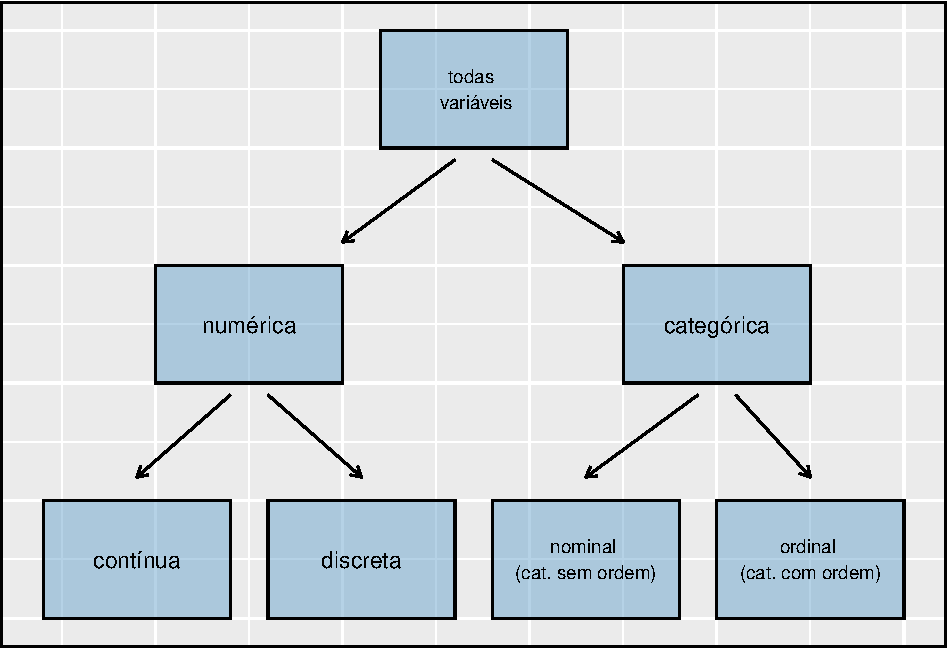
\includegraphics{_main_files/figure-latex/variables-1.pdf}
\caption{\label{fig:variables}Repartição das variáveis em seus respectivos tipos.}
\end{figure}

\begin{example}
\protect\hypertarget{exm:unnamed-chunk-4}{}{\label{exm:unnamed-chunk-4} }Os dados foram coletados sobre os alunos em um curso de estatística. Três variáveis foram registradas para cada aluno: número de irmãos, altura do aluno e se o aluno já havia feito um curso de estatística. Classifique cada uma das variáveis como numérica contínua, numérica discreta ou categórica.
\end{example}

O número de irmãos e a altura dos alunos representam variáveis numéricas. Como o número de irmãos é uma contagem, ele é discreto. Altura varia continuamente, por isso é uma variável numérica contínua. A última variável classifica os alunos em duas categorias - aqueles que fizeram e aqueles que não fizeram um curso de estatística -- o que torna essa variável categórica.

\begin{center}\rule{0.5\linewidth}{0.5pt}\end{center}

\begin{exercise}
\protect\hypertarget{exr:unnamed-chunk-5}{}{\label{exr:unnamed-chunk-5} }Considere as variáveis \textbf{grupo} e \textbf{resultado} (a 30 dias) do estudo \emph{stent} na Seção \ref{basicExampleOfStentsAndStrokes}. São estas variáveis numéricas ou categóricas?\footnote{Existem apenas dois valores possíveis para cada variável e, em ambos os casos, descrevem categorias. Assim, cada um é uma variável categórica.}
\end{exercise}

\begin{center}\rule{0.5\linewidth}{0.5pt}\end{center}

\hypertarget{variableRelations}{%
\subsection{Relações entre variáveis}\label{variableRelations}}

Muitas análises são motivadas por um pesquisador que procura uma relação entre duas ou mais variáveis. Um cientista social pode gostar de responder a algumas das seguintes perguntas:

\begin{itemize}
\item
  Os gastos federais, em média, são maiores ou menores nos condados com altas taxas de pobreza?
\item
  Se a variável \emph{casa própria} for menor que a média nacional em um município, a percentagem de estruturas de várias unidades naquele município provavelmente estará acima ou abaixo da média nacional?
\item
  Quais municípios têm uma renda média maior: aqueles que decretam uma ou mais proibições de fumar ou aqueles que não a decretaram?
\end{itemize}

Para responder a essas perguntas, os dados devem ser coletados, como o conjunto de dados \texttt{condado} mostrado na Tabela \ref{tab:countyDF}. Examinar as estatísticas-resumo poderia fornecer \emph{insights} para cada uma das três perguntas sobre condados. Além disso, os gráficos podem ser usados para resumir visualmente os dados e são úteis para responder a essas perguntas também. \textbf{Gráficos de dispersão} são um tipo de gráfico usado para estudar a relação entre duas variáveis numéricas. A Figura \ref{fig:countyfedspendVsPoverty} compara as variáveis \texttt{fed\_spend} e \texttt{poverty}.

Cada ponto representa um único condado. Por exemplo, o ponto realçado corresponde ao Condado 1088 no conjunto de dados: Owsley County, Kentucky, que tinha uma taxa de pobreza de 41,5\% e gastos federais de \$21,50 per capita. O gráfico de dispersão sugere uma relação entre as duas variáveis: os municípios com alta taxa de pobreza também tendem a ter um pouco mais de gastos federais. Podemos pensar em por que essa relação existe e investigar cada ideia para determinar qual é a explicação mais razoável.

\begin{figure}
\centering
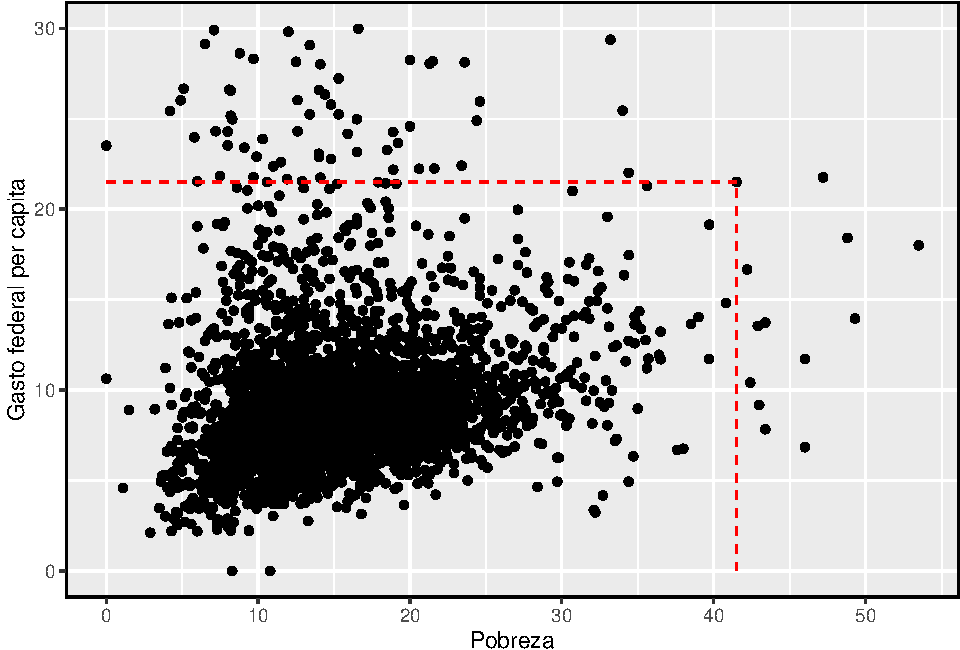
\includegraphics{_main_files/figure-latex/countyfedspendVsPoverty-1.pdf}
\caption{\label{fig:countyfedspendVsPoverty}Um gráfico de dispersão mostrando fed\_spend contra poverty.}
\end{figure}

\begin{center}\rule{0.5\linewidth}{0.5pt}\end{center}

\begin{exercise}
\protect\hypertarget{exr:unnamed-chunk-6}{}{\label{exr:unnamed-chunk-6} }Examine as variáveis no banco de dados \texttt{email50}, descritos na Tabela \ref{tab:email50Variables}. Crie duas perguntas sobre os relacionamentos entre essas variáveis que são de seu interesse.\footnote{Duas perguntas de exemplo: (1) A intuição sugere que, se houver muitas quebras de linha em um email, haverá também muitos caracteres: isso é verdade? (2) Existe uma conexão entre se um formato de email é texto simples (versus HTML) e se é uma mensagem de spam?}
\end{exercise}

\begin{center}\rule{0.5\linewidth}{0.5pt}\end{center}

Diz-se que as duas variáveis estão associadas porque o gráfico mostra um padrão discernível. Quando duas variáveis mostram alguma conexão umas com as outras, elas são chamadas variáveis \textbf{associadas}. Variáveis associadas também podem ser chamadas variáveis \emph{dependentes} e vice-versa.

\begin{example}
\protect\hypertarget{exm:unnamed-chunk-7}{}{\label{exm:unnamed-chunk-7} }Este exemplo examina a relação entre a proporção de casa própria e a porcentagem de unidades em estruturas de multi-unidades (por exemplo, apartamentos e condomínios), que é visualizada usando um gráfico de dispersão na Figura \ref{fig:multiunitsVsOwnership}. Essas variáveis estão associadas?
\end{example}

\begin{figure}
\centering
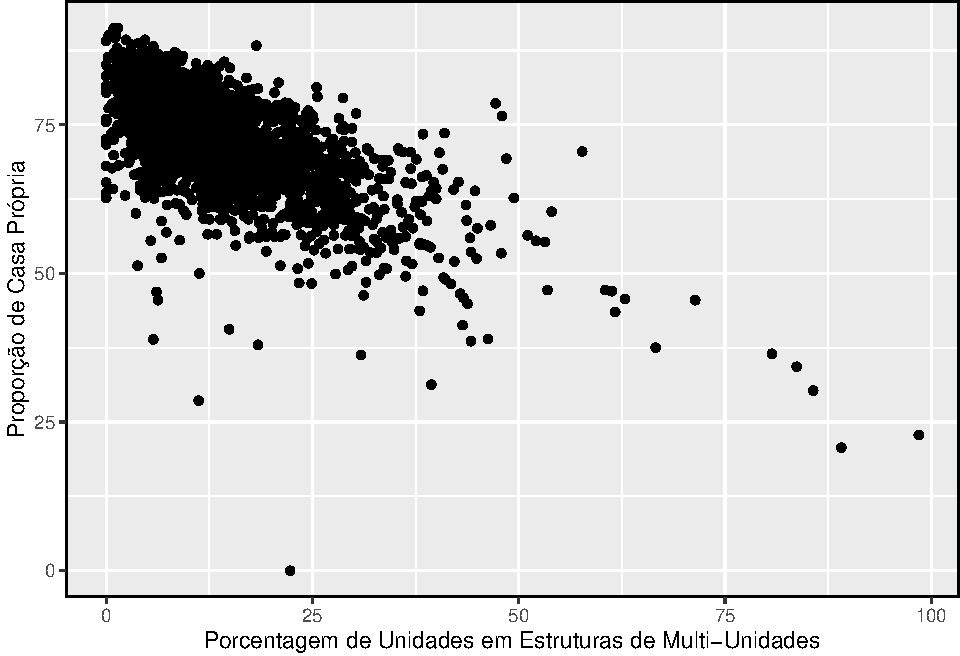
\includegraphics{_main_files/figure-latex/multiunitsVsOwnership-1.pdf}
\caption{\label{fig:multiunitsVsOwnership}Gráfico de dispersão entre a proporção de casa própria e a porcentagem de unidades eem estruturas de multi-unidades}
\end{figure}

Parece que quanto maior a fração de unidades em estruturas com várias unidades, menor a taxa de casa própria. Como existe alguma relação entre as variáveis, elas estão associadas.

Porque há uma tendência de queda na Figura \ref{fig:multiunitsVsOwnership} -- municípios com mais unidades em estruturas de várias unidades estão associados a uma menor casa própria -- essas variáveis são consideradas \textbf{associadas negativamente}. Uma \textbf{associação positiva} é mostrada na relação entre as variáveis \emph{poverty} e \emph{fed\_spend} representadas na Figura \ref{fig:countyfedspendVsPoverty}, onde os municípios com maiores taxas de pobreza tendem a receber mais gastos federais per capita.
Se duas variáveis não estão associadas, então elas são \textbf{independentes}. Ou seja, duas variáveis são independentes se não houver relação evidente entre as duas.

Associado ou independente, não ambos: Um par de variáveis estão relacionadas de alguma forma (associadas) ou não (independentes). Nenhum par de variáveis são associadas e independentes.

\hypertarget{overviewOfDataCollectionPrinciples}{%
\section{Visão geral dos princípios de coleta de dados}\label{overviewOfDataCollectionPrinciples}}

O primeiro passo na condução de pesquisas é identificar tópicos ou questões que devem ser investigados. Uma pergunta de pesquisa claramente apresentada é útil para identificar quais assuntos ou casos devem ser estudados e quais variáveis são importantes. Também é importante considerar \emph{como} os dados são coletados para que sejam confiáveis e ajudem a atingir as metas de pesquisa.

\hypertarget{populationsAndSamples}{%
\subsection{Populações e amostras}\label{populationsAndSamples}}

Considere as três perguntas de pesquisa a seguir:

\begin{itemize}
\item
  Qual é o teor médio de mercúrio no peixe-espada do Oceano Atlântico?
\item
  Nos últimos 5 anos, qual é o tempo médio para concluir um curso para alunos de graduação da Duke?
\item
  Um novo medicamento reduz o número de mortes em pacientes com doença cardíaca grave?
\end{itemize}

Cada questão de pesquisa refere-se a uma \textbf{população alvo}. Na primeira questão, a população alvo é todo o peixe-espada no oceano Atlântico, e cada peixe representa um caso. Muitas vezes, é muito caro coletar dados para todos os casos em uma população. Em vez disso, uma amostra é obtida. A \textbf{amostra} representa um subconjunto dos casos e geralmente é uma pequena fração da população. Por exemplo, 60 peixes-espada (ou algum outro número) na população podem ser selecionados, e esses dados de amostra podem ser usados para fornecer uma estimativa da média populacional e responder à pergunta da pesquisa.

\begin{center}\rule{0.5\linewidth}{0.5pt}\end{center}

\begin{exercise}
\protect\hypertarget{exr:identifyingThePopulationForTwoQuestionsInPopAndSampSubsection}{}{\label{exr:identifyingThePopulationForTwoQuestionsInPopAndSampSubsection} }Para a segunda e terceira questões acima, identifique a população alvo e o que representa um caso individual.\footnote{Observe que a primeira pergunta só é relevante para os alunos que concluem o curso; a média não pode ser calculada usando um aluno que nunca terminou sua graduação Assim, apenas os alunos de graduação da Duke que se formaram nos últimos cinco anos representam casos na população em questão. Cada um desses estudantes representaria um caso individual. Uma pessoa com doença cardíaca grave representa um caso. A população inclui todas as pessoas com doença cardíaca grave.}
\end{exercise}

\begin{center}\rule{0.5\linewidth}{0.5pt}\end{center}

\hypertarget{anecdotalEvidenceSubsection}{%
\subsection{Evidência anedótica}\label{anecdotalEvidenceSubsection}}

Considere as seguintes respostas possíveis para as três questões de pesquisa:

\begin{itemize}
\item
  Um homem no noticiário tem envenenamento por mercúrio por comer espadarte, então a concentração média de mercúrio em espadarte deve ser perigosamente alta.
\item
  Eu conheci dois alunos que levaram mais de sete anos para se formar na Duke, então deve levar mais tempo para se formar na Duke do que em muitas outras faculdades.
\item
  O pai da minha amiga teve um ataque cardíaco e morreu depois que eles lhe deram uma nova droga para doença cardíaca, então a droga não deve funcionar.
\end{itemize}

Cada conclusão é baseada em dados. No entanto, existem dois problemas. Primeiro, os dados representam apenas um ou dois casos. Em segundo lugar, e mais importante, não está claro se esses casos são realmente representativos da população. Dados coletados dessa maneira casual são chamados \textbf{evidência anedótica}.

\begin{figure}
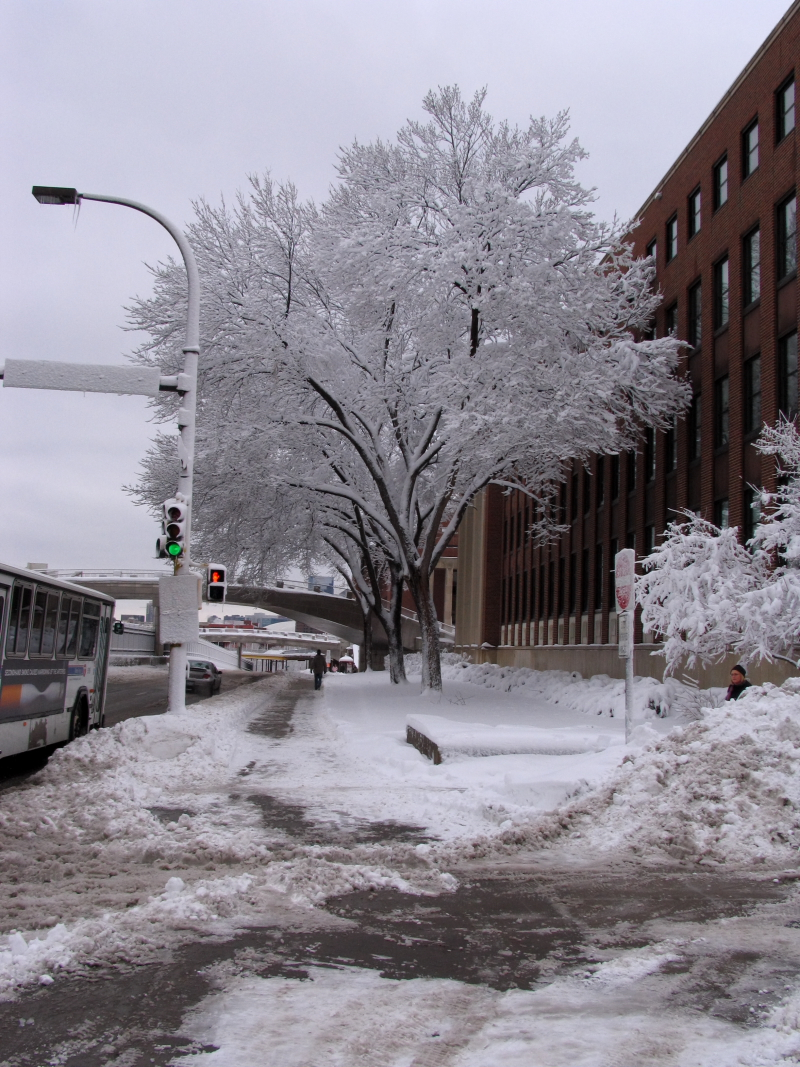
\includegraphics[width=11.11in]{images/c1/mnWinter} \caption{Em fevereiro de 2010, alguns especialistas da mídia citaram uma grande tempestade de neve como evidência válida contra o aquecimento global. Como o comediante Jon Stewart apontou: É uma tempestade, em uma região, de um país.}\label{fig:mnWinter}
\end{figure}

Evidência anedótica: Tenha cuidado com os dados coletados de maneira aleatória. Tal evidência pode ser verdadeira e verificável, mas pode apenas representar casos extraordinários.

A evidência anedótica é tipicamente composta de casos incomuns que lembramos com base em suas características marcantes. Por exemplo, é mais provável que nos lembremos das duas pessoas que conhecemos que levaram sete anos para se formar do que as outras seis que se formaram em quatro anos. Em vez de olhar para os casos mais incomuns, devemos examinar uma amostra de muitos casos que representam a população.

\hypertarget{popSampling}{%
\subsection{Amostragem de uma população}\label{popSampling}}

Podemos tentar estimar o tempo para a graduação de alunos de graduação da Duke nos últimos 5 anos, coletando uma amostra de alunos. Todos os graduados nos últimos 5 anos representam a população, e graduados que são amostra. Em geral, procuramos sempre \textbf{aleatoriamente} selecionar uma amostra de uma população. O tipo mais básico de seleção aleatória é equivalente a como os sorteios são conduzidos. Por exemplo, na seleção de graduados, poderíamos escrever o nome de cada graduado em um bilhete de rifa e comprar 100 ingressos. Os nomes selecionados representariam uma amostra aleatória de 100 graduados.

\begin{figure}
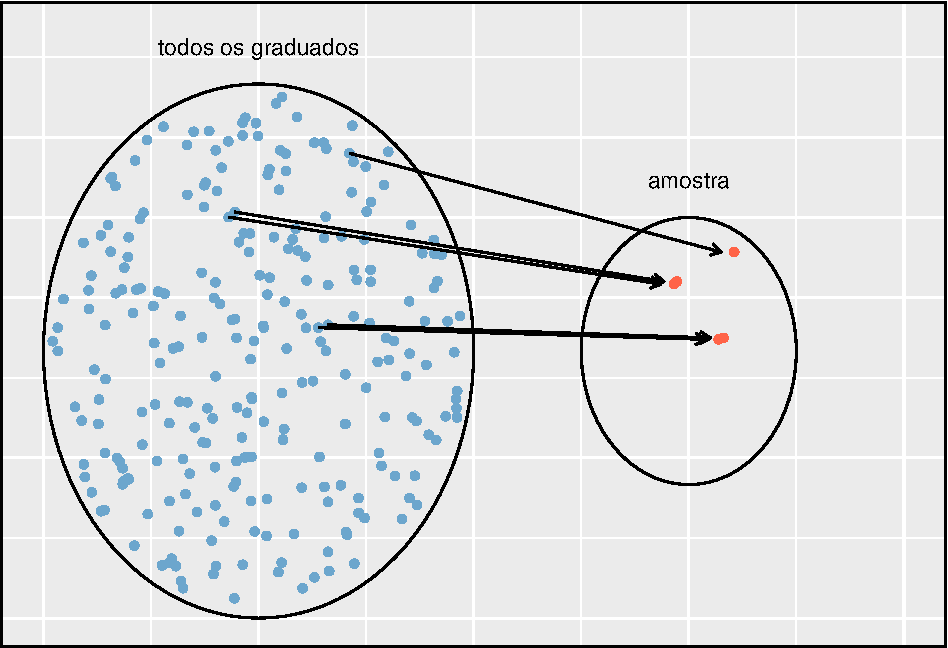
\includegraphics[width=0.8\linewidth]{_main_files/figure-latex/popToSampleGraduates-1} \caption{Neste gráfico, cinco graduados são selecionados aleatoriamente da população para serem incluídos na amostra.}\label{fig:popToSampleGraduates}
\end{figure}

Por que escolher uma amostra aleatoriamente? Por que não escolher apenas uma amostra à mão? Considere o seguinte cenário.

\begin{example}
\protect\hypertarget{exm:unnamed-chunk-8}{}{\label{exm:unnamed-chunk-8} }Suponha que perguntemos a um aluno que esteja se formando em nutrição para selecionar vários graduados para o estudo. Que tipo de alunos você acha que ela pode colecionar? Você acha que sua amostra seria representativa de todos os graduados?
\end{example}

Talvez ela escolheria um número desproporcional de graduados em campos relacionados à saúde. Ou talvez a seleção dela fosse bem representativa da população. Ao selecionar amostras manualmente, corremos o risco de escolher uma amostra \textbf{tendenciosa}, mesmo que esse preconceito não seja intencional ou difícil de discernir.

\begin{figure}
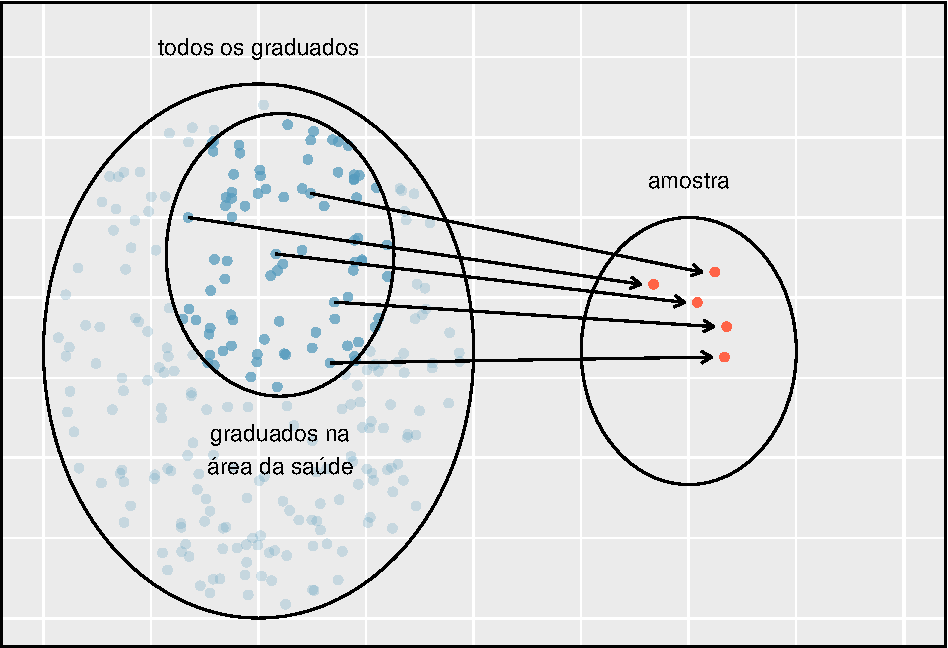
\includegraphics[width=0.8\linewidth]{_main_files/figure-latex/popToSubSampleGraduates-1} \caption{Em vez de amostragem de todos os graduados igualmente, um nutricionista pode, inadvertidamente, escolher graduados com cursos relacionados à saúde de forma desproporcional.}\label{fig:popToSubSampleGraduates}
\end{figure}

Se alguém tiver permissão para escolher exatamente quais graduados foram incluídos na amostra, é totalmente possível que a amostra possa ser distorcida aos interesses dessa pessoa, o que pode ser totalmente não intencional. Isso introduz um \emph{viés} na amostra. Uma amostragem aleatória ajuda a resolver esse problema. A amostra aleatória mais básica é chamada de \textbf{amostra aleatória simples}, e é equivalente a usar um sorteio para selecionar casos. Isso significa que cada caso na população tem uma chance igual de ser incluído e não há conexão implícita entre os casos na amostra.

\begin{quote}
Às vezes, uma amostra aleatória simples é difícil de implementar e um método alternativo é útil. Um método substituto é uma \textbf{amostra sistemática}, onde um caso é amostrado depois de deixar um número fixo de outros, digamos 10 outros casos, passar. Como essa abordagem usa um mecanismo que não é facilmente sujeito a vieses pessoais, geralmente produz uma amostra razoavelmente representativa. Este livro se concentrará em amostras aleatórias, já que o uso de amostras sistemáticas é incomum e requer considerações adicionais do contexto.
\end{quote}

O ato de pegar uma amostra aleatória simples ajuda a minimizar o viés. No entanto, o preconceito pode surgir de outras formas. Mesmo quando as pessoas são escolhidas aleatoriamente, por exemplo, deve-se ter cautela se a \emph{não resposta} está alta. Por exemplo, se apenas 30\% das pessoas amostradas aleatoriamente para uma pesquisa realmente responderem, então não está claro se os resultados são representativos de toda a população. Esse termo \textbf{viés de não resposta} pode distorcer resultados.

\begin{figure}
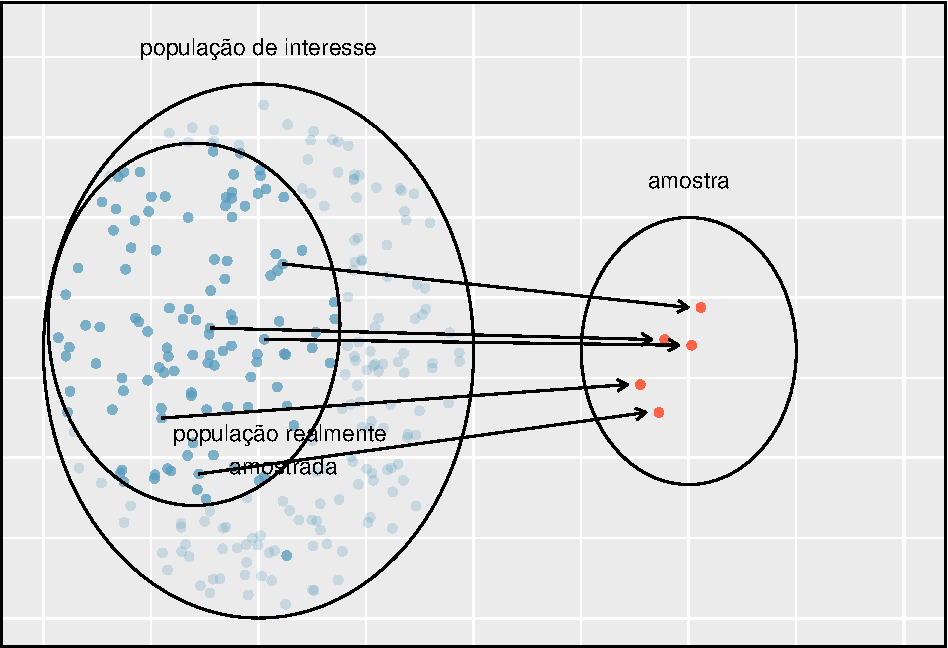
\includegraphics[width=0.8\linewidth]{_main_files/figure-latex/surveySample-1} \caption{Devido à possibilidade de não resposta, os estudos de pesquisa só podem atingir um determinado grupo dentro da população. É difícil, e muitas vezes impossível, corrigir completamente esse problema.}\label{fig:surveySample}
\end{figure}

Outro método comum é uma \textbf{amostra de conveniência}, onde os indivíduos que são facilmente acessíveis têm maior probabilidade de serem incluídos na amostra. Por exemplo, se uma pesquisa política for feita em pessoas que andam no Bronx, isso não representará toda a cidade de Nova York. Muitas vezes é difícil discernir qual subpopulação uma amostra de conveniência representa.

\begin{center}\rule{0.5\linewidth}{0.5pt}\end{center}

\begin{exercise}
\protect\hypertarget{exr:unnamed-chunk-9}{}{\label{exr:unnamed-chunk-9} }Podemos acessar facilmente classificações de produtos, vendedores e empresas por meio de sites. Essas classificações são baseadas apenas naquelas pessoas que fazem de tudo para fornecer uma classificação. Se 50\% das avaliações on-line de um produto forem negativas, você acha que isso significa que 50\% dos compradores estão insatisfeitos com o produto?\footnote{As respostas variam. A partir de nossas próprias experiências, acreditamos que as pessoas tendem a reclamar mais sobre os produtos que caíram abaixo das expectativas do que as que têm o desempenho esperado. Por esse motivo, suspeitamos que haja um viés negativo nas classificações de produtos em sites como a Amazon. Entretanto, como nossas experiências podem não ser representativas, também mantemos uma mente aberta.}
\end{exercise}

\begin{center}\rule{0.5\linewidth}{0.5pt}\end{center}

\hypertarget{explanatoryAndResponse}{%
\subsection{Variáveis explicativas e de resposta}\label{explanatoryAndResponse}}

Considere a pergunta que foi feita para o conjunto de dados \texttt{condado} na seção \ref{variableRelations}:

\begin{itemize}
\tightlist
\item
  Os gastos federais, em média, são maiores ou menores nos condados com altas taxas de pobreza?
\end{itemize}

Se suspeitarmos que a pobreza possa afetar os gastos em um país, então a pobreza é a variável \textbf{explanatória} e o gasto federal é a variável \textbf{resposta} no relacionamento. \footnote{Às vezes, a variável explicativa é chamada de variável independente e a variável resposta é chamada de variável dependente. No entanto, isso se torna confuso, pois um par de variáveis pode ser independente ou dependente, de modo que evitamos essa linguagem. Se houver muitas variáveis, pode ser possível considerar algumas delas como variáveis explicativas.}

\textbf{Dica}: Variáveis explicativas e resposta: Para identificar a variável explicativa em um par de variáveis, identifique qual das duas é suspeita de afetar a outra e planeje uma análise apropriada.

\textbf{Cuidado:} associação não implica causalidade: Rotular variáveis como \emph{explicativa} e \emph{resposta} não garante que a relação entre os dois seja realmente causal, mesmo se houver uma associação identificada entre as duas variáveis. Usamos esses rótulos apenas para rastrear qual variável suspeitamos que afeta a outra.

Em alguns casos, não há variável explicativa ou resposta.

Considere a seguinte pergunta da seção \ref{variableRelations}:

\begin{itemize}
\tightlist
\item
  Se a casa própria for menor que a média nacional em um município, a percentagem de estruturas de várias unidades naquele município provavelmente estará acima ou abaixo da média nacional?
\end{itemize}

É difícil decidir qual dessas variáveis deve ser considerada a variável explicativa e resposta, ou seja, a direção é ambígua, portanto, nenhum rótulo explicativo ou de resposta é sugerido aqui.

\hypertarget{introObservationalExperimentStudies}{%
\subsection{Introduzindo estudos observacionais e experimentos}\label{introObservationalExperimentStudies}}

Existem dois tipos principais de coleta de dados: estudos observacionais e experimentos.

Pesquisadores realizam um \textbf{estudo observacional} quando coletam dados de uma maneira que não interfere diretamente na forma como os dados surgem. Por exemplo, os pesquisadores podem coletar informações por meio de pesquisas, revisar registros médicos ou da empresa ou seguir uma \emph{coorte} de muitos indivíduos semelhantes para estudar por que certas doenças podem se desenvolver. Em cada uma dessas situações, os pesquisadores simplesmente observam os dados que surgem. Em geral, estudos observacionais podem fornecer evidências de uma associação natural entre variáveis, mas não podem, por si só, mostrar uma conexão causal.

Quando os pesquisadores querem investigar a possibilidade de uma conexão causal, eles conduzem um \textbf{experimento}. Geralmente, haverá uma variável explicativa e uma variável de resposta. Por exemplo, podemos suspeitar que administrar uma droga reduzirá a mortalidade em pacientes com ataque cardíaco no ano seguinte. Para verificar se existe realmente uma conexão causal entre a variável explicativa e a resposta, os pesquisadores coletarão uma amostra de indivíduos e os dividirão em grupos. Os indivíduos em cada grupo são atribuídos a um tratamento. Quando os indivíduos são aleatoriamente designados para um grupo, o experimento é chamado de \textbf{experimento aleatório}. Por exemplo, cada paciente com ataque cardíaco no estudo pode ser aleatoriamente designado, talvez jogando uma moeda, em um dos dois grupos: o primeiro grupo recebe um \emph{placebo} e o segundo recebe o medicamento. Veja o estudo de caso na Seção \ref{basicExampleOfStentsAndStrokes} para outro exemplo de um experimento, embora esse estudo não empregou um placebo.

Associação \(\neq\) causa: Em geral, a associação não implica causalidade, e a causalidade só pode ser inferida a partir de um experimento randomizado.

\hypertarget{observationalStudiesSamplingStrategies}{%
\section{Estudos observacionais e estratégias de amostragem}\label{observationalStudiesSamplingStrategies}}

\hypertarget{observationalStudies}{%
\subsection{Estudos observacionais}\label{observationalStudies}}

Geralmente, os dados em estudos observacionais são coletados apenas pelo monitoramento do que ocorre, enquanto os experimentos exigem que a variável explicativa primária em um estudo seja atribuída para cada sujeito pelos pesquisadores.

Fazer conclusões causais baseadas em experimentos é geralmente razoável. No entanto, fazer as mesmas conclusões causais com base em dados observacionais pode ser traiçoeiro e não é recomendado. Assim, estudos observacionais são geralmente suficientes apenas para mostrar associações.

\begin{center}\rule{0.5\linewidth}{0.5pt}\end{center}

\begin{exercise}
\protect\hypertarget{exr:sunscreenLurkingexampleux2cux20echo=T}{}{(\#exr:sunscreenLurkingexample, echo=T) }Suponha que um estudo observacional acompanhasse o uso de protetor solar e câncer de pele, e descobriu-se que quanto mais protetor solar alguém usava, maior a probabilidade de a pessoa ter câncer de pele. Isso significa que o protetor solar \textbf{causa} câncer de pele?\footnote{Não. Veja o parágrafo seguinte ao exercício para uma explicação.}
\end{exercise}

\begin{center}\rule{0.5\linewidth}{0.5pt}\end{center}

Algumas pesquisas anteriores nos dizem que usar protetor solar realmente reduz o risco de câncer de pele, então talvez haja outra variável que pode explicar essa associação hipotética entre uso de filtro solar e câncer de pele. Uma informação importante que está ausente é a exposição ao sol. Se alguém está no sol o dia todo, ela é mais propensa a usar protetor solar e mais chances de ter câncer de pele. A exposição ao sol não é contabilizada na simples investigação.

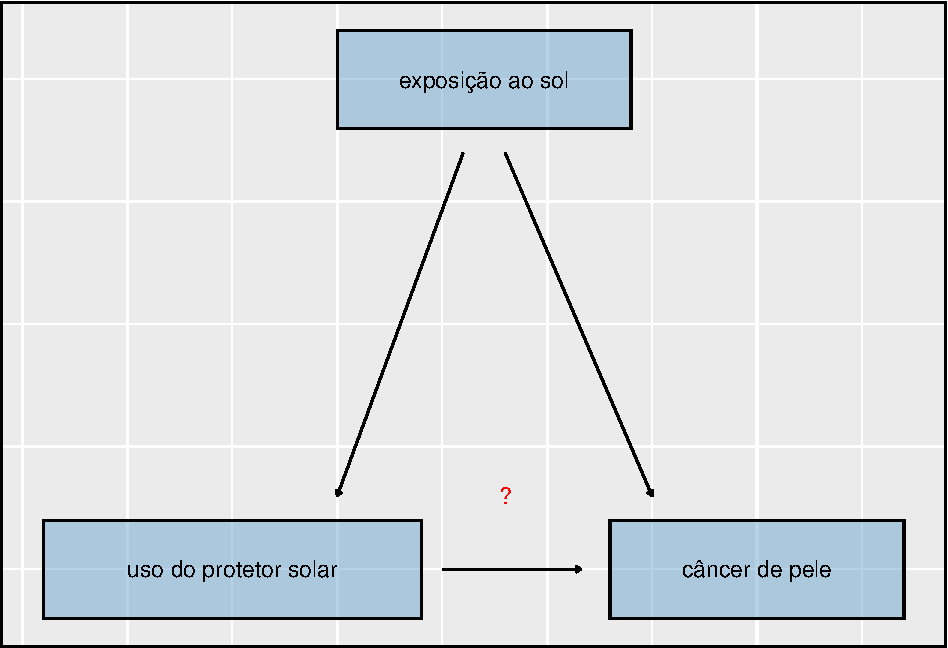
\includegraphics{_main_files/figure-latex/unnamed-chunk-10-1.pdf}

A exposição ao sol é o que é chamado de \textbf{variável de confusão}\footnote{Também chamado de variável oculta, fator de confusão ou um confundidor.}. Que é uma variável correlacionada com as variáveis explicativas e respostas. Enquanto um método para justificar a tomada de conclusões causais a partir de estudos observacionais é exaurir a busca por variáveis de confusão, não há garantia de que todas as variáveis confusas possam ser examinadas ou medidas.

Da mesma forma, o conjunto de dados \texttt{condado} é um estudo observacional com variáveis confundidoras, e seus dados não podem ser facilmente usados para fazer conclusões causais.

\begin{center}\rule{0.5\linewidth}{0.5pt}\end{center}

\begin{exercise}
\protect\hypertarget{exr:unnamed-chunk-11}{}{\label{exr:unnamed-chunk-11} }A Figura \ref{fig:multiunitsVsOwnership} mostra uma associação negativa entre a taxa de propriedade e a porcentagem de estruturas de múltiplas unidades em um município. No entanto, não é razoável concluir que existe uma relação causal entre as duas variáveis. Sugira uma ou mais outras variáveis que possam explicar a relação visível na Figura \ref{fig:multiunitsVsOwnership}.\footnote{As respostas vão variar. A densidade populacional pode ser importante. Se um município é muito denso, isso pode exigir que uma fração maior de residentes viva em estruturas com várias unidades. Além disso, a alta densidade pode contribuir para o aumento do valor da propriedade, tornando a posse de imóvel inviável para muitos moradores.}
\end{exercise}

\begin{center}\rule{0.5\linewidth}{0.5pt}\end{center}

Estudos observacionais vêm em duas formas: estudos prospectivos e retrospectivos. Um \textbf{estudo prospectivo} identifica os indivíduos e coleta informações à medida que os eventos se desdobram. Por exemplo, pesquisadores médicos podem identificar e acompanhar um grupo de indivíduos semelhantes durante muitos anos para avaliar as possíveis influências do comportamento no risco de câncer. Um exemplo de tal estudo é \emph{The Nurses 'Health Study}, iniciado em 1976 e expandido em 1989\footnote{www.channing.harvard.edu/nhs}. Este estudo prospectivo recruta enfermeiros registrados e, em seguida, coleta dados deles usando questionários. \textbf{Estudos retrospectivos} coletam dados após os eventos terem ocorrido, por exemplo os pesquisadores podem revisar os eventos passados nos registros médicos. Alguns conjuntos de dados, como \texttt{condado}, podem conter variáveis coletadas prospectiva e retrospectivamente. Os governos locais coletam prospectivamente algumas variáveis à medida que os eventos se desenrolam (por exemplo, vendas de varejo) enquanto o governo federal coletou retrospectivamente outras durante o censo de 2010 (por exemplo, contagem da população do condado).

\hypertarget{fourSamplingMethods}{%
\subsection{Quatro métodos de amostragem (tópico especial)}\label{fourSamplingMethods}}

Quase todos os métodos estatísticos são baseados na noção de aleatoriedade implícita. Se os dados observacionais não forem coletados em uma estrutura aleatória de uma população, esses métodos estatísticos -- as estimativas e os erros associados às estimativas -- não são confiáveis. Aqui, consideramos quatro técnicas de amostragem aleatória: amostragem simples, estratificada, por conglomerados e de múltiplos estágios. Figuras \ref{fig:simplestratified} e @ref(fig:clustermultistage\} fornecem representações gráficas dessas técnicas.

\begin{figure}
\centering
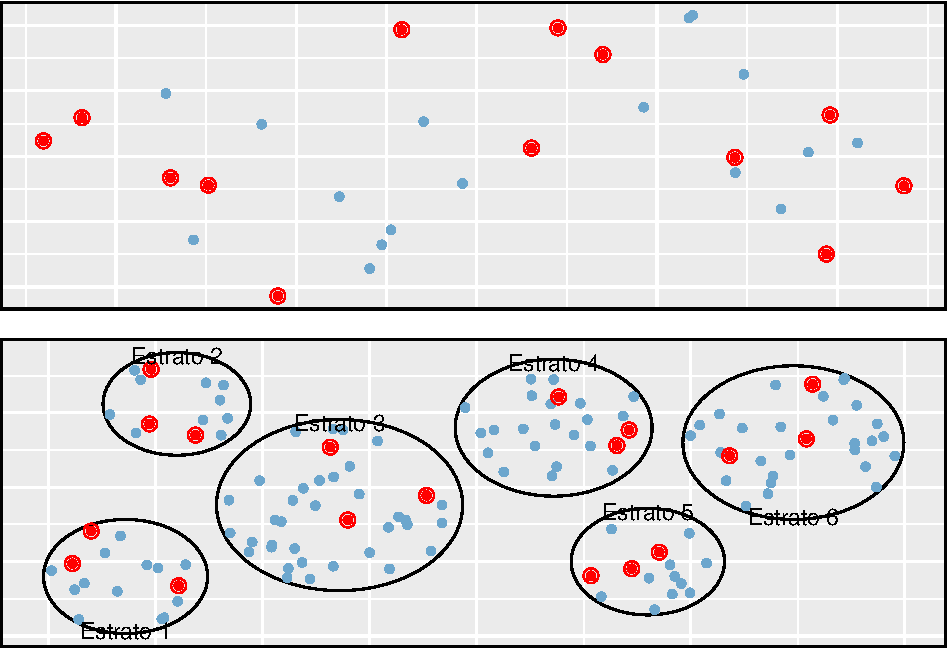
\includegraphics{_main_files/figure-latex/simplestratified-1.pdf}
\caption{\label{fig:simplestratified}Exemplos de amostragem simples e amostragem estratificada. No painel superior, a amostragem aleatória simples foi usada para selecionar aleatoriamente os 18 casos. No painel inferior, utilizou-se amostragem estratificada: os casos foram agrupados em estratos e, em seguida, a amostragem aleatória simples foi feita para cada estrato.}
\end{figure}

A \textbf{amostragem aleatória simples} é provavelmente a forma mais intuitiva de amostragem aleatória. Considere os salários dos jogadores da Major League Baseball (MLB), onde cada jogador é membro de uma das 30 equipes da liga. Para pegar uma simples amostra aleatória de 120 jogadores de beisebol e seus salários da temporada de 2010, poderíamos escrever os nomes dos 828 jogadores daquela temporada em pedaços de papel, colocar os pedaços de papel num balde, sacudir o balde até termos certeza de que os nomes estão todos misturados, depois escreva os nomes tirados até que tenhamos a amostra de 120 jogadores. Em geral, uma amostra é chamada de \emph{aleatória simples} se cada caso na população tiver uma chance igual de ser incluído na amostra final e saber que um caso é incluído em uma amostra não fornece informações úteis sobre quais outros casos estão incluídos.

A \textbf{amostragem Estratificada} é uma estratégia de amostragem de `divisão e conquista'. A população é dividida em grupos chamados \textbf{estratos}. Os estratos são escolhidos de modo que os casos semelhantes sejam agrupados e, em seguida, um segundo método de amostragem, geralmente amostragem aleatória simples, é empregado dentro de cada estrato. No exemplo do salário no beisebol, as equipes poderiam representar os estratos, já que algumas equipes têm muito mais dinheiro (até 4 vezes mais!). Então, podemos aleatoriamente amostrar 4 jogadores de cada equipe para um total de 120 jogadores.

A amostragem estratificada é especialmente útil quando os casos em cada estrato são muito semelhantes em relação ao resultado de interesse. A desvantagem é que analisar dados de uma amostra estratificada é uma tarefa mais complexa do que analisar dados de uma amostra aleatória simples. Os métodos de análise introduzidos neste livro precisariam ser estendidos para analisar os dados coletados usando amostragem estratificada.

\begin{example}
\protect\hypertarget{exm:unnamed-chunk-12}{}{\label{exm:unnamed-chunk-12} }Por que seria bom que os casos dentro de cada estrato fossem muito semelhantes?
\end{example}

Podemos obter uma estimativa mais estável para a subpopulação em um estrato, se os casos forem muito semelhantes. Essas estimativas aprimoradas para cada subpopulação nos ajudarão a construir uma estimativa confiável para toda a população.

Em uma \textbf{amostragem por conglomerados}, nós dividimos a população em muitos grupos, chamados \textbf{clusters}. Em seguida, amostramos um número fixo de clusters e incluímos todas as observações de cada um desses clusters na amostra. Uma \textbf{amostra de vários estágios} é como uma amostra de cluster, mas em vez de manter todas as observações em cada cluster, coletamos uma amostra aleatória em cada cluster selecionado.

\begin{figure}
\centering
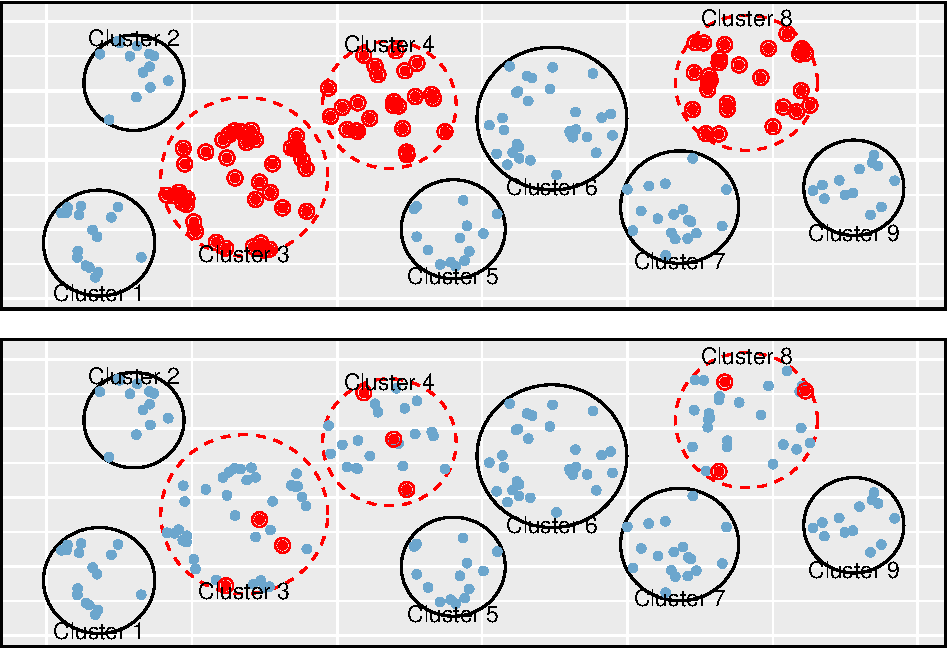
\includegraphics{_main_files/figure-latex/clustermultistage-1.pdf}
\caption{\label{fig:clustermultistage}Exemplos de comglomerados e amostragem de múltiplos estágios. No painel superior, foi usada a amostragem por conglomerados. Aqui, os dados foram colocados em nove clusters, três desses clusters foram amostrados e todas as observações dentro desses três clusters foram incluídas na amostra. No painel inferior, foi utilizada amostragem multiestágios. Diferencia-se da amostragem por conglomerados na dos clusters selecionados, selecionamos aleatoriamente um subconjunto de cada cluster a ser incluído na amostra.}
\end{figure}

Às vezes, a amostragem por conglomerados ou em múltiplos estágios pode ser mais econômica do que as técnicas alternativas de amostragem. Além disso, ao contrário da amostragem estratificada, essas abordagens são mais úteis quando há muita variabilidade caso a caso dentro de um cluster, mas os próprios clusters não parecem muito diferentes um do outro. Por exemplo, se os bairros representarem clusters, então o cluster ou a amostragem multi-estágio funcionará melhor quando os bairros forem muito diversos. Uma desvantagem desses métodos é que as técnicas de análise mais avançadas são normalmente necessárias, embora os métodos neste livro possam ser estendidos para lidar com esses dados.

\begin{example}
\protect\hypertarget{exm:unnamed-chunk-13}{}{\label{exm:unnamed-chunk-13} }Suponha que estamos interessados em estimar a taxa de malária em uma parte densamente tropical da Indonésia rural. Aprendemos que existem 30 aldeias naquela parte da selva indonésia, cada uma mais ou menos semelhante à seguinte. Nosso objetivo é testar 150 indivíduos por malária. Qual método de amostragem deve ser empregado?
\end{example}

Uma simples amostra aleatória provavelmente atrairia indivíduos de todas as 30 aldeias, o que poderia tornar a coleta de dados extremamente cara. A amostragem estratificada seria um desafio, pois não está claro como construiríamos estratos de indivíduos semelhantes. No entanto, a amostragem por conglomerados ou a amostragem em múltiplos estágios parece ser uma boa ideia. Se decidirmos usar a amostragem de múltiplos estágios, podemos selecionar aleatoriamente metade das aldeias e, em seguida, selecionar aleatoriamente 10 pessoas de cada uma. Isso provavelmente reduziria nossos custos de coleta de dados substancialmente em comparação a uma amostra aleatória simples, e essa abordagem ainda nos forneceria informações confiáveis.

\hypertarget{experimentsSection}{%
\section{Experimentos}\label{experimentsSection}}

Estudos em que os pesquisadores atribuem tratamentos a casos são chamados de \textbf{experimentos}. Quando esta tarefa inclui aleatoriedade, por exemplo, usando uma moeda para decidir qual tratamento um paciente recebe, é chamado de \textbf{experimento aleatório}. Experimentos aleatórios são fundamentalmente importantes quando se tenta mostrar uma conexão causal entre duas variáveis.

\hypertarget{experimentalDesignPrinciples}{%
\section{Princípios do design experimental}\label{experimentalDesignPrinciples}}

Experimentos randomizados são geralmente construídos em quatro princípios.

\begin{itemize}
\item
  \textbf{Controlando:} Os pesquisadores atribuem tratamentos aos casos e fazem o melhor que podem para \emph{controlar} quaisquer outras diferenças nos grupos. Por exemplo, quando os pacientes tomam uma droga em forma de pílula, alguns pacientes tomam a pílula com apenas um gole de água enquanto outros a tomam com um copo inteiro de água. Para controlar o efeito do consumo de água, o médico pode pedir a todos os pacientes que bebam um copo de água com a pílula.
\item
  \textbf{Randomização:} Pesquisadores randomizam os pacientes em grupos de tratamento para responder por variáveis que não podem ser controladas. Por exemplo, alguns pacientes podem ser mais suscetíveis a uma doença do que outros devido a seus hábitos alimentares. A randomização dos pacientes no grupo de tratamento ou controle ajuda a nivelar essas diferenças e também evita que vieses acidentais entrem no estudo.
\item
  \textbf{Replicação:} Quanto mais casos os pesquisadores observam, mais precisamente eles podem estimar o efeito da variável explicativa sobre a resposta. Em um único estudo, nós \emph{replicamos} coletando uma amostra suficientemente grande. Além disso, um grupo de cientistas pode replicar um estudo inteiro para verificar uma descoberta anterior.
\item
  \textbf{Bloqueio:} Os pesquisadores às vezes sabem ou suspeitam que variáveis, além do tratamento, influenciam a resposta. Nestas circunstâncias, eles podem primeiro agrupar os indivíduos com base nesta variável \emph{bloqueadora} e depois randomiza os casos dentro de cada bloco para os grupos de tratamento. Esta estratégia é frequentemente referida como \emph{bloqueio}. Por exemplo, se estivermos analisando o efeito de um medicamento nos ataques cardíacos, podemos dividir os pacientes no estudo em blocos de baixo risco e alto risco, e então atribuir aleatoriamente metade dos pacientes de cada bloco ao grupo controle e outra metade para o grupo de tratamento, como mostrado na Figura \ref{fig:figureShowingBlocking}. Essa estratégia garante que cada grupo de tratamento tenha um número igual de pacientes de baixo risco e alto risco.
\end{itemize}

\begin{figure}
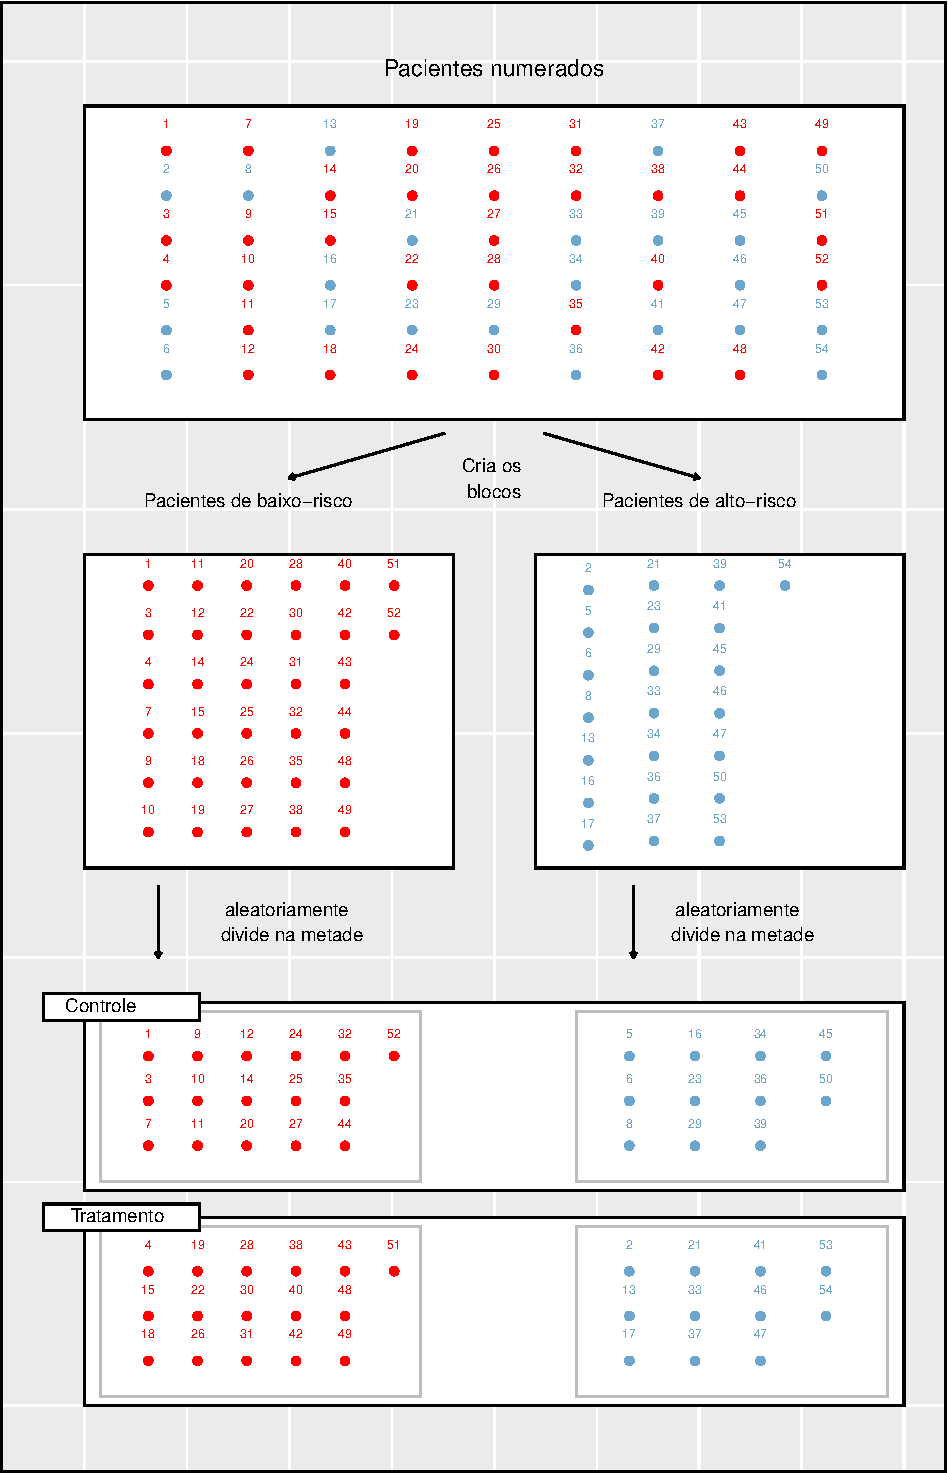
\includegraphics[height=1\textheight]{_main_files/figure-latex/figureShowingBlocking-1} \caption{Bloqueio usando uma variável representando risco do paciente. Os pacientes são primeiro divididos em blocos de baixo risco e alto risco, em seguida, cada bloco é uniformemente separado nos grupos de tratamento usando randomização. Essa estratégia garante uma representação igual dos pacientes em cada grupo de tratamento, tanto nas categorias de baixo risco quanto de alto risco.}\label{fig:figureShowingBlocking}
\end{figure}

É importante incorporar os três primeiros princípios de projeto experimental em qualquer estudo, e este livro descreve os métodos aplicáveis para analisar dados de tais experimentos. O bloqueio é uma técnica um pouco mais avançada, e os métodos estatísticos neste livro podem ser estendidos para analisar os dados coletados usando o bloqueio.

\hypertarget{biasInHumanExperiments}{%
\subsection{Redução do viés em experimentos em humanos}\label{biasInHumanExperiments}}

Experimentos aleatórios são o padrão ouro para a coleta de dados, mas não garantem uma perspectiva imparcial sobre as relações de causa e efeito em todos os casos. Estudos humanos são exemplos perfeitos onde o preconceito pode surgir involuntariamente. Aqui nós reconsideramos um estudo em que um novo medicamento foi usado para tratar pacientes com ataque cardíaco\footnote{Grupo de Pesquisa Experimental de Reinfarto Anturano. 1980. Sulfinpirazona na prevenção de morte súbita após infarto do miocárdio. New England Journal of Medicine 302 (5):250-256.}. Em particular, os pesquisadores queriam saber se a droga reduziu as mortes em pacientes.

Esses pesquisadores planejaram um experimento aleatório porque queriam tirar conclusões causais sobre o efeito da droga. Os voluntários do estudo\footnote{Os assuntos humanos são freqüentemente chamados de pacientes, voluntários ou participantes do estudo.} Foram aleatoriamente colocados em dois grupos de estudo. Um grupo, o \textbf{grupo de tratamento}, recebeu o medicamento. O outro grupo, chamado de \textbf{grupo controle}, não recebeu nenhum tratamento medicamentoso.

Coloque-se no lugar de uma pessoa no estudo. Se você estiver no grupo de tratamento, receberá uma nova droga que você espera que o ajude. Por outro lado, uma pessoa do outro grupo não recebe a droga e senta-se à toa, esperando que sua participação não aumente seu risco de morte. Essas perspectivas sugerem que existem dois efeitos: o de interesse é a eficácia do medicamento e o segundo é um efeito emocional difícil de quantificar.

Os pesquisadores geralmente não estão interessados no efeito emocional, o que pode influenciar o estudo. Para contornar esse problema, os pesquisadores não querem que os pacientes saibam em que grupo estão. Quando os pesquisadores mantêm os pacientes desinformados sobre seu tratamento, o estudo é considerado como sendo \textbf{cego}. Mas há um problema: se um paciente não receber um tratamento, ele saberá que está no grupo de controle. A solução para este problema é dar tratamentos falsos aos pacientes do grupo controle. Um tratamento falso é chamado de \textbf{placebo}, e um placebo eficaz é a chave para tornar um estudo verdadeiramente cego. Um exemplo clássico de placebo é uma pílula de açúcar que é feita para se parecer com a pílula de tratamento atual. Muitas vezes, um placebo resulta em uma melhora leve, mas real, nos pacientes. Este efeito foi apelidado de \emph{efeito placebo}.

Os pacientes não são os únicos que devem ser cegados: médicos e pesquisadores podem acidentalmente enviesar um estudo. Quando um médico sabe que um paciente recebeu o tratamento real, ele pode, inadvertidamente, dar mais atenção ou cuidado ao paciente do que um paciente que ele sabe que está tomando placebo. Para se proteger contra esse viés, que de novo foi descoberto ter um efeito mensurável em alguns casos, a maioria dos estudos modernos emprega a configuração \textbf{duplo-cego} onde médicos ou pesquisadores que interagem com pacientes são, assim como os pacientes, inconscientes de quem está ou não recebendo o tratamento\footnote{Há sempre alguns pesquisadores envolvidos no estudo que sabem quais pacientes estão recebendo o tratamento. No entanto, eles não interagem com os pacientes do estudo e não informam aos profissionais de saúde cegos que estão recebendo o tratamento.}.

\begin{center}\rule{0.5\linewidth}{0.5pt}\end{center}

\begin{exercise}
\protect\hypertarget{exr:unnamed-chunk-14}{}{\label{exr:unnamed-chunk-14} }Olhe para o estudo na Seção \ref{basicExampleOfStentsAndStrokes} onde os pesquisadores estavam testando se \emph{stents} foram eficazes na redução de acidentes vasculares cerebrais em pacientes de risco. Isso é uma experiência? O estudo foi cego? Foi duplo-cego? \footnote{Os pesquisadores atribuíram os pacientes em seus grupos de tratamento, então este estudo foi um experimento. No entanto, os pacientes puderam distinguir o tratamento que receberam, portanto este estudo não foi cego. O estudo não poderia ser duplo-cego, uma vez que não era cego.}
\end{exercise}

\begin{center}\rule{0.5\linewidth}{0.5pt}\end{center}

\hypertarget{numericalData}{%
\section{Examinando dados numéricos}\label{numericalData}}

Nesta seção, serão introduzidos técnicas para explorar e resumir variáveis numéricas. Os conjuntos de dados \texttt{email50} e \texttt{condado} da Seção \ref{dataBasics} fornecem ricas oportunidades para exemplos. Lembre-se de que os resultados de variáveis numéricas são números nos quais é razoável realizar operações aritméticas básicas. Por exemplo, a variável \textbf{pop2010}, que representa as populações dos municípios em 2010, é numérica, já que podemos discutir sensivelmente a diferença ou a proporção das populações em dois municípios. Por outro lado, os códigos de área e CEPs não são numéricos e sim variáveis categóricas.

\hypertarget{scatterPlots}{%
\subsection{Gráficos de dispersão para dados pareados}\label{scatterPlots}}

Um \textbf{gráfico de dispersão} fornece uma visão caso a caso de dados para duas variáveis numéricas. Na Figura \ref{fig:countyfedspendVsPoverty}, um gráfico de dispersão foi usado para examinar como os gastos federais e a pobreza estavam relacionados no conjunto de dados \texttt{condado}. Outro gráfico de dispersão é mostrado na Figura \ref{fig:email50LinesCharacters}, comparando o número de quebras de linha e número de caracteres em e-mails para o conjunto de dados \texttt{email50}. Em qualquer gráfico de dispersão, cada ponto representa um único caso. Como há 50 casos em \texttt{email50}, há 50 pontos na Figura \ref{fig:email50LinesCharacters}.

\begin{figure}
\centering
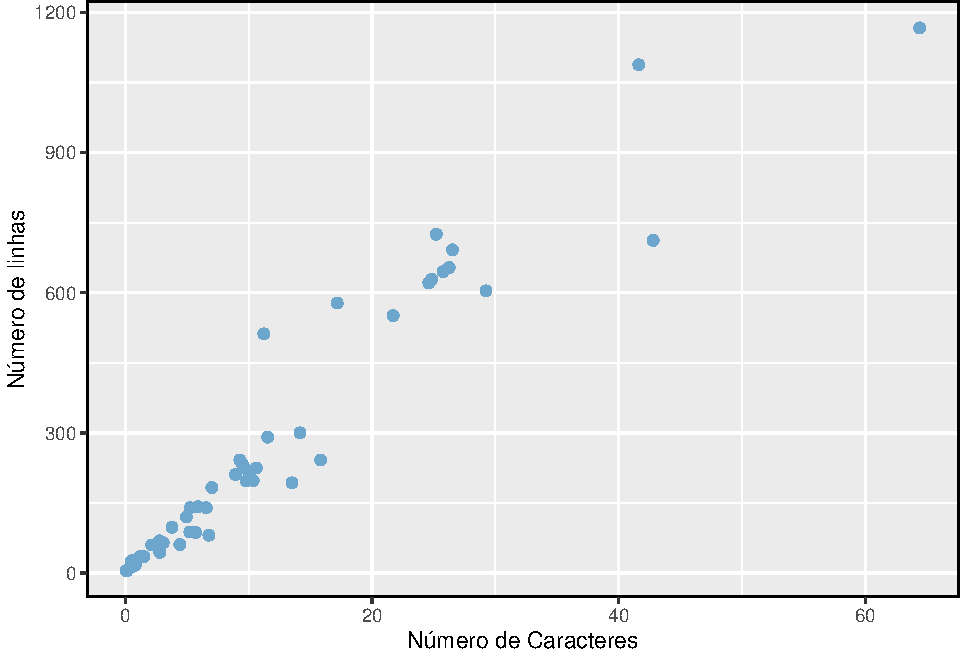
\includegraphics{_main_files/figure-latex/email50LinesCharacters-1.pdf}
\caption{\label{fig:email50LinesCharacters}Um gráfico de dispersão entre as variáveis número de quebras de linhas e número de caractéres em emails para o conjunto de dados email50}
\end{figure}

Para colocar o número de caracteres em perspectiva, este parágrafo possui 363 caracteres. Olhando para a Figura \ref{fig:email50LinesCharacters}, parece que alguns e-mails são incrivelmente detalhados! Após uma investigação mais aprofundada, descobriríamos que a maioria dos e-mails longos usa o formato HTML, o que significa que a maioria dos caracteres desses e-mails é usada para formatar o e-mail em vez de fornecer texto.

\begin{center}\rule{0.5\linewidth}{0.5pt}\end{center}

\begin{exercise}
\protect\hypertarget{exr:unnamed-chunk-15}{}{\label{exr:unnamed-chunk-15} }O que os gráficos de dispersão revelam sobre os dados e como eles podem ser úteis?\footnote{As respostas podem variar. Os diagramas de dispersão são úteis para identificar rapidamente associações relacionadas a variáveis, independentemente de essas associações virem na forma de tendências simples ou se esses relacionamentos são mais complexos.}
\end{exercise}

\begin{center}\rule{0.5\linewidth}{0.5pt}\end{center}

\begin{example}
\protect\hypertarget{exm:unnamed-chunk-16}{}{\label{exm:unnamed-chunk-16} }Considere um novo conjunto de dados de 54 carros com duas variáveis: preço do veículo e peso\footnote{www.amstat.org/publications/jse/v1n1/datasets.lock.html}. Um gráfico de dispersão do preço do veículo versus peso é mostrado na Figura \ref{fig:carsPriceVsWeight}. O que pode ser dito sobre a relação entre essas variáveis?
\end{example}

\begin{figure}
\centering
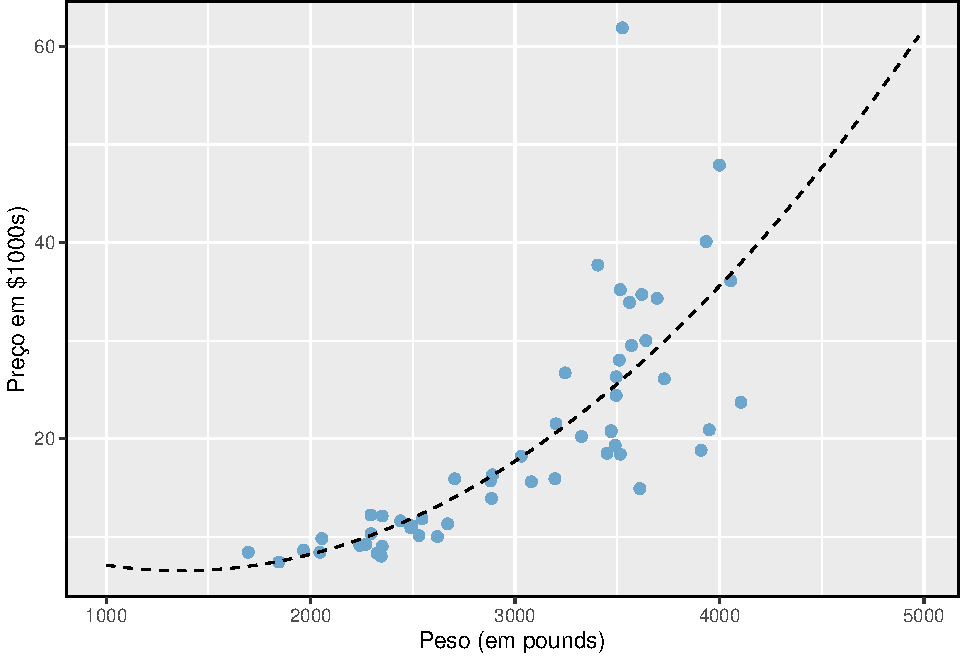
\includegraphics{_main_files/figure-latex/carsPriceVsWeight-1.pdf}
\caption{\label{fig:carsPriceVsWeight}Um gráfico de dispersão de price versus weight para 54 carros.}
\end{figure}

A relação é evidentemente não-linear, conforme destacado pela linha tracejada. Isso é diferente dos gráficos de dispersão anteriores que vimos, como na Figura \ref{fig:countyfedspendVsPoverty} e Figura \ref{fig:email50LinesCharacters}, que mostram relações que são muito lineares.

\begin{center}\rule{0.5\linewidth}{0.5pt}\end{center}

\begin{exercise}
\protect\hypertarget{exr:unnamed-chunk-17}{}{\label{exr:unnamed-chunk-17} }Descreva duas variáveis que teriam uma associação em forma de ferradura em um gráfico de dispersão.\footnote{Considere o caso em que seu eixo vertical representa algo ``bom'' e seu eixo horizontal representa algo que só é bom com moderação. A saúde e o consumo de água se encaixam nessa descrição, já que a água se torna tóxica quando consumida em quantidades excessivas.}
\end{exercise}

\begin{center}\rule{0.5\linewidth}{0.5pt}\end{center}

\hypertarget{dotPlot}{%
\subsection{Gráfico de pontos e a média}\label{dotPlot}}

Às vezes, duas variáveis são demais: apenas uma variável pode ser de interesse. Nesses casos, um gráfico de pontos fornece as informações mais básicas. Um \textbf{gráfico de pontos} é um gráfico de dispersão de uma variável. Um exemplo usando o número de caracteres de 50 e-mails é mostrado na Figura \ref{fig:emailCharactersDotPlot}. Uma versão empilhada deste gráfico de pontos é mostrada na Figura \ref{fig:emailCharactersDotPlotStacked}.

\begin{figure}
\centering
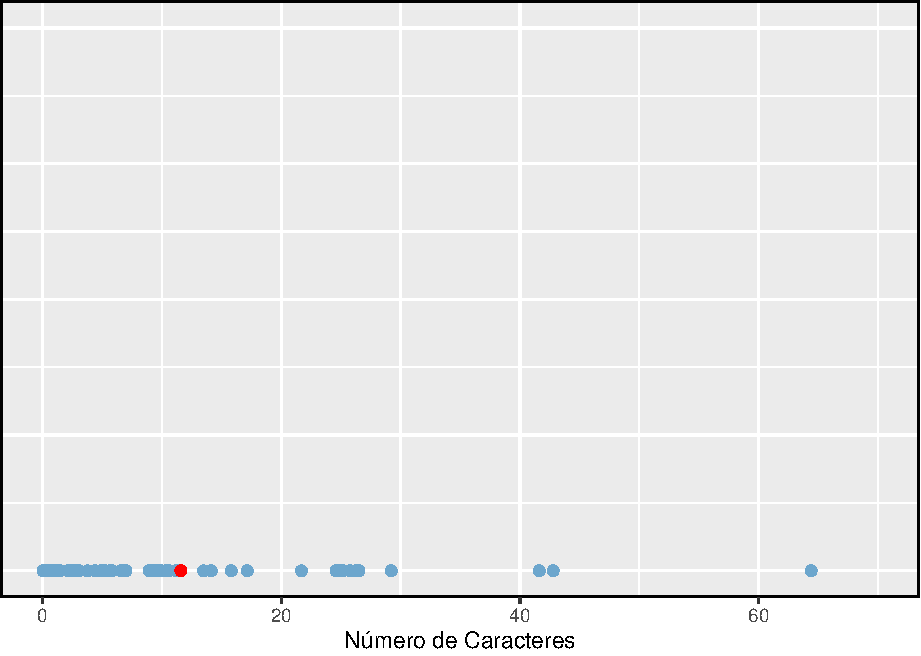
\includegraphics{_main_files/figure-latex/emailCharactersDotPlot-1.pdf}
\caption{\label{fig:emailCharactersDotPlot}Um gráfico de pontos da variável número de caracteres para o banco de dados email50}
\end{figure}

\begin{figure}
\centering
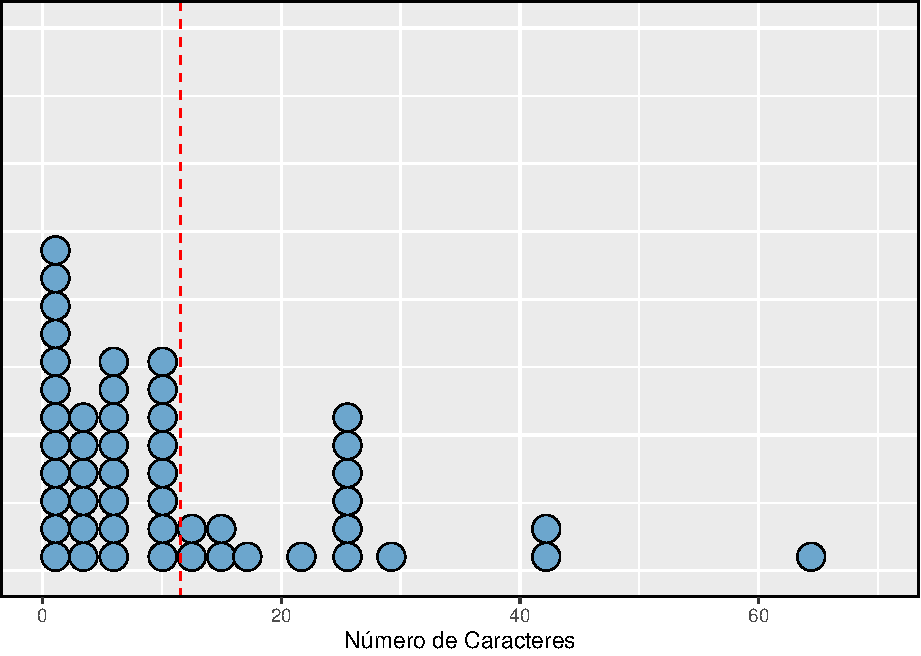
\includegraphics{_main_files/figure-latex/emailCharactersDotPlotStacked-1.pdf}
\caption{\label{fig:emailCharactersDotPlotStacked}Um gráfico de pontos empilhados do número de caracteres para o banco de dados email50.}
\end{figure}

A \textbf{média}, é uma maneira comum de medir o centro de uma \textbf{distribuição} de dados. Para encontrar o número médio de caracteres nos 50 e-mails, somamos todas as contagens de caracteres e dividimos pelo número de e-mails. Para conveniência computacional, o número de caracteres é listado em milhares e arredondado para o primeiro decimal.

\begin{eqnarray}
\bar{x} = \frac{21.7 + 7.0 + \cdots + 15.8}{50} = 11.6
\label{eq:sampleMeanEquation}
\end{eqnarray}

A média da amostra é frequentemente rotulada de \(\bar{x}\). A letra \(x\) está sendo usada como um marcador genérico para a variável de interesse, \texttt{var\_char}, e a barra sobre o \(x\) comunica que o número médio de caracteres nos 50 e-mails foi de 11.6. É útil pensar na média como o ponto de equilíbrio da distribuição. A média da amostra é mostrada como um ponto vermelho na Figura \ref{fig:emailCharactersDotPlot} e uma linha pontilhada vermelha na Figura \ref{fig:emailCharactersDotPlotStacked}.

Média: A média amostral de uma variável numérica é calculada como a soma de todas as observações divididas pelo número de observações:

\begin{eqnarray}
\bar{x} = \frac{x_1+x_2+\cdots+x_n}{n}
\label{eq:meanEquation}
\end{eqnarray}

onde \(x_1, x_2, \dots, x_n\) representa os \(n\) valores observados.

\begin{center}\rule{0.5\linewidth}{0.5pt}\end{center}

\begin{exercise}
\protect\hypertarget{exr:unnamed-chunk-18}{}{\label{exr:unnamed-chunk-18} }Examine as Equações \eqref{eq:sampleMeanEquation} e \eqref{eq:meanEquation} a seguir. Com o que \(x_1\) corresponde? E \(x_2\)? Você pode inferir um significado geral para o que \(x_i\) pode representar?\footnote{\(x_1\) corresponde ao número de caracteres no primeiro e-mail da amostra (21.7, em milhares), \(x_2\) ao número de caracteres na amostra segundo e-mail (7.0, em milhares) e \(x_i\) corresponde ao número de caracteres no i-ésimo e-mail no conjunto de dados.}
\end{exercise}

\begin{center}\rule{0.5\linewidth}{0.5pt}\end{center}

\begin{center}\rule{0.5\linewidth}{0.5pt}\end{center}

\begin{exercise}
\protect\hypertarget{exr:unnamed-chunk-19}{}{\label{exr:unnamed-chunk-19} }O que era \(n\) nessa amostra de e-mails?\footnote{O tamanho da amostra era \(n=50\).}
\end{exercise}

\begin{center}\rule{0.5\linewidth}{0.5pt}\end{center}

O conjunto de dados \texttt{email} representa uma amostra de uma população maior de emails recebidos em janeiro e março. Podemos calcular uma média para essa população da mesma maneira que a média da amostra. No entanto, a média populacional tem um rótulo especial: \(\mu\). O símbolo \(\mu\) é a letra grega \emph{mu} e representa a média de todas as observações na população. Às vezes, um subscrito, como \(_x\), é utilizado para representar a que variável a média populacional se refere, \(\mu_x\).

\begin{example}
\protect\hypertarget{exm:unnamed-chunk-20}{}{\label{exm:unnamed-chunk-20} }O número médio de caracteres em todos os e-mails pode ser estimado usando os dados de um amostra. Com base na amostra de 50 emails, qual seria uma estimativa razoável de \(\mu_x\), o número médio de caracteres em todos os emails no conjunto de dados? (Lembre-se de que \texttt{email50} é uma amostra de \texttt{email}.)
\end{example}

A média da amostra, 11.600, pode fornecer uma estimativa razoável de \(\mu_x\). Embora este número não seja perfeito, ele fornece uma \textbf{estimativa pontual} da média da população. Além disso, desenvolveremos ferramentas para caracterizar a precisão das estimativas pontuais, e descobriremos que as estimativas pontuais baseadas em amostras maiores tendem a ser mais precisas do que aquelas baseadas em amostras menores.

\begin{example}
\protect\hypertarget{exm:wtdMeanOfIncome}{}{\label{exm:wtdMeanOfIncome} }Podemos querer calcular a renda média por pessoa nos EUA. Para fazer isso, podemos pensar primeiro em obter a média da renda per capita nos 3143 condados do conjunto de dados \texttt{condado}. Qual seria uma abordagem melhor?
\end{example}

O banco de dados \texttt{condado} é especial, pois cada condado na verdade representa muitas pessoas individuais. Se fôssemos simplesmente fazer a média através da variável \texttt{renda}, estaríamos tratando municípios com 5.000 e 5.000.000 residentes igualmente nos cálculos. Em vez disso, devemos calcular a renda total de cada município, somar todos os totais dos municípios e dividir pelo número de pessoas em todos os municípios. Se concluíssemos essas etapas com os dados de \texttt{condado}, descobriríamos que a renda per capita dos EUA é de \$27.348,43. Se tivéssemos calculado a média simples de renda per capita entre os países, o resultado teria sido de apenas \$ 22.504,70!

O Exemplo \ref{exm:wtdMeanOfIncome} usou o que é chamado de \textbf{média ponderada}, que não será um tópico chave neste livro. No entanto, fornecemos um suplemento on-line sobre meios ponderados para leitores interessados:

\begin{center}
[www.openintro.org/d?f=wtdmean]
\end{center}

\hypertarget{histogramsAndShape}{%
\subsection{Histogramas e forma}\label{histogramsAndShape}}

Os gráficos de pontos mostram o valor exato de cada observação. Isso é útil para pequenos conjuntos de dados, mas eles podem se tornar difíceis de ler com amostras maiores. Em vez de mostrar o valor de cada observação, preferimos pensar no valor como pertencente a um \emph{intervalo}. Por exemplo, no conjunto de dados \texttt{email50}, criamos uma tabela de contagens para o número de casos com contagens de caracteres entre 0 e 5.000, depois o número de casos entre 5.000 e 10.000 e assim por diante. Observações que caem no limite de um intervalo (por exemplo, 5.000) são alocadas no intervalo inferior. Esta tabulação é mostrada na Tabela \ref{tab:binnedNumCharTable}. Essas contagens binárias são plotadas como barras na Figura \ref{fig:email50NumCharHist} no que é chamado de \textbf{histograma}, que se assemelha ao gráfico de pontos empilhados mostrado na Figura \ref{fig:emailCharactersDotPlotStacked}.

\begin{table}

\caption{\label{tab:binnedNumCharTable}As contagens para os dados número de caracteres em forma de intervalos}
\centering
\begin{tabular}[t]{l|c|c|c|c|c|c|c|c|c}
\hline
  & 0-5 & 5-10 & 10-15 & 15-20 & 20-25 & 25-30 & ··· & 55-60 & 60-65\\
\hline
contagem & 19 & 12 & 6 & 2 & 3 & 5 & ··· & 0 & 1\\
\hline
\end{tabular}
\end{table}

\begin{figure}
\centering
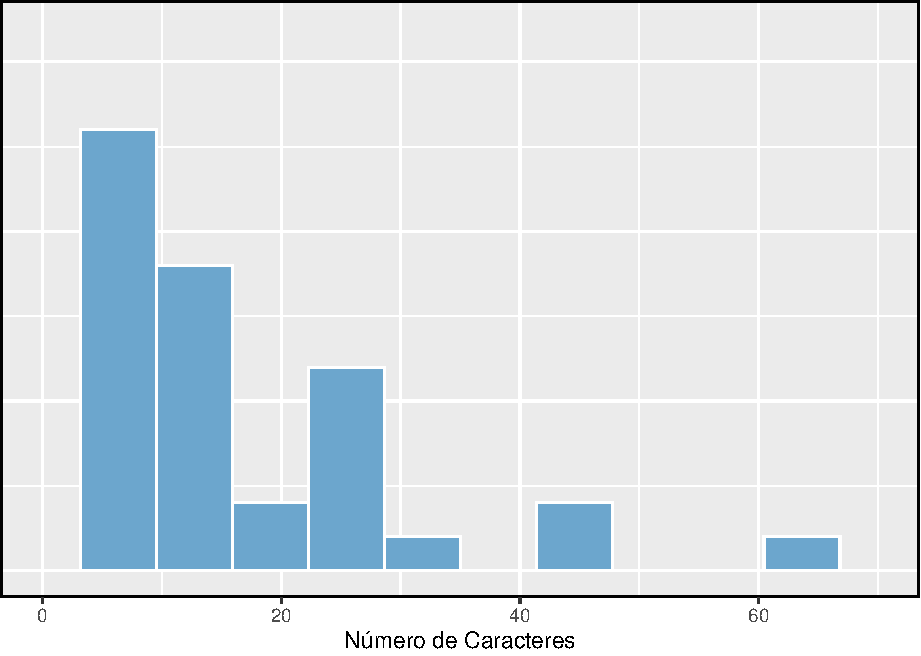
\includegraphics{_main_files/figure-latex/email50NumCharHist-1.pdf}
\caption{\label{fig:email50NumCharHist}Um histograma da variavel num\_char. Esta distribuição é muito fortemente inclinada para a direita}
\end{figure}

Histogramas fornecem uma visão da \textbf{densidade de dados}. Barras mais altas representam onde os dados são relativamente mais comuns. Por exemplo, existem muito mais e-mails com menos de 20.000 caracteres que e-mails com pelo menos 20.000 no conjunto de dados. As barras facilitam ver como a densidade dos dados muda em relação ao número de caracteres.

Os histogramas são especialmente convenientes para descrever a forma da distribuição. A Figura \ref{fig:email50NumCharHist} mostra que a maioria dos e-mails tem um número relativamente pequeno de caracteres, enquanto poucos e-mails têm um número muito grande de caracteres. Quando os dados se arrastam para a direita dessa maneira e têm uma maior cauda para direita, a forma é dita ser \textbf{assimétrico a direita}\footnote{Outras maneiras de descrever dados que estão inclinados para a direita: inclinado para a direita ou assimetria positiva.}.

Os conjuntos de dados com a característica inversa -- uma cauda longa e fina à esquerda -- são considerados \textbf{assimétricos a esquerda}. Nós também dizemos que tal distribuição tem uma cauda longa e esquerda. Conjuntos de dados que mostram aproximadamente iguais em ambas as direções são chamados simétricos.

Cauda longa para identificar inclinação: Quando os dados desaparecem em uma direção, a distribuição tem uma \emph{causa longa}.

\begin{center}\rule{0.5\linewidth}{0.5pt}\end{center}

\begin{exercise}
\protect\hypertarget{exr:unnamed-chunk-21}{}{\label{exr:unnamed-chunk-21} }Dê uma olhada nos gráficos de pontos na Figuras \ref{fig:emailCharactersDotPlot} e \ref{fig:emailCharactersDotPlotStacked}. Você pode ver a inclinação nos dados? É mais fácil ver a inclinação neste histograma ou os gráficos de pontos?\footnote{A inclinação é visível em todos os três gráficos, embora o gráfico de pontos seja o menos útil. O gráfico e o histograma de pontos empilhados são visualizações úteis para identificar distorções.}
\end{exercise}

\begin{center}\rule{0.5\linewidth}{0.5pt}\end{center}

\begin{center}\rule{0.5\linewidth}{0.5pt}\end{center}

\begin{exercise}
\protect\hypertarget{exr:unnamed-chunk-22}{}{\label{exr:unnamed-chunk-22} }Além da média (desde que foi rotulado), o que você pode ver nos gráficos de pontos que você não pode ver no histograma?\footnote{Contagens de caracteres para e-mails individuais.}
\end{exercise}

\begin{center}\rule{0.5\linewidth}{0.5pt}\end{center}

Além de verificar se uma distribuição é assimétrica ou simétrica, os histogramas podem ser usados para identificar modas. Uma \textbf{moda} é representada por um pico proeminente na distribuição.\footnote{Outra definição de moda, que não é normalmente usada em estatísticas, é o valor com maior número de ocorrências. É comum ter observações com o mesmo valor em um conjunto de dados, o que torna essa outra definição inútil para muitos conjuntos de dados reais.} Há apenas um pico proeminente no histograma de \texttt{\_char}.

A Figura \ref{fig:singleBiMultiModalPlots} mostra histogramas que têm um, dois ou três picos proeminentes. Tais distribuições são chamadas unimodal, bimodal e multimodal, respectivamente. Qualquer distribuição com mais de 2 picos proeminentes é chamada multimodal. Observe que havia um pico proeminente na distribuição unimodal com um segundo pico menos proeminente que não foi contado, uma vez que só difere de seus intervalos vizinhos por algumas observações.

\begin{figure}
\centering
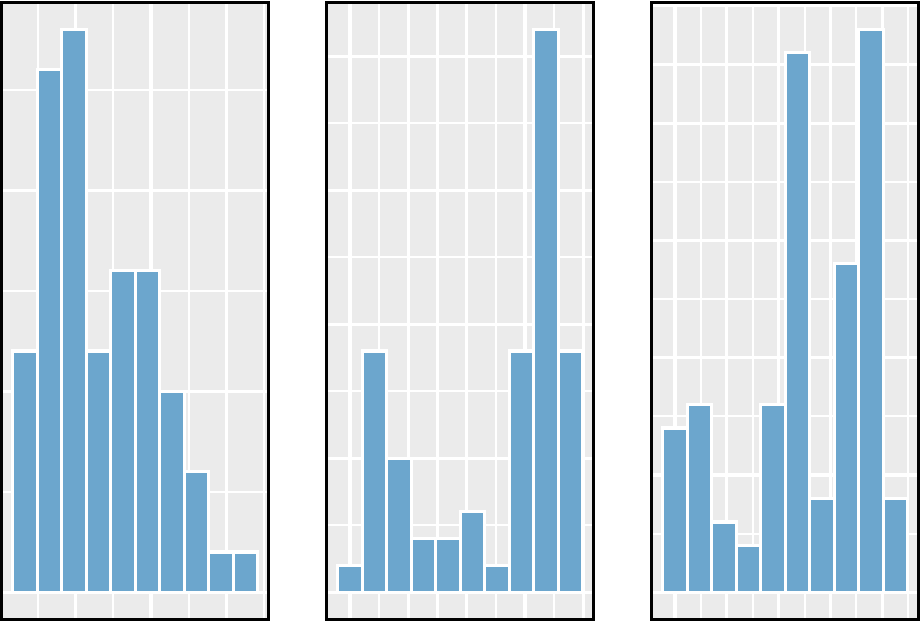
\includegraphics{_main_files/figure-latex/singleBiMultiModalPlots-1.pdf}
\caption{\label{fig:singleBiMultiModalPlots}Contando apenas picos proeminentes, as distribuições são (da esquerda para a direita) unimodal, bimodal e multimodal. Note que dissemos que o gráfico da esquerda é unimodal intencionalmente. Isso ocorre porque estamos contando picos proeminentes, e não apenas um pico.}
\end{figure}

\begin{center}\rule{0.5\linewidth}{0.5pt}\end{center}

\begin{exercise}
\protect\hypertarget{exr:unnamed-chunk-23}{}{\label{exr:unnamed-chunk-23} }A Figura \ref{fig:email50NumCharHist} revela apenas um moda proeminente no número de caracteres. A distribuição é unimodal, bimodal ou multimodal?\footnote{Unimodal}
\end{exercise}

\begin{center}\rule{0.5\linewidth}{0.5pt}\end{center}

\begin{center}\rule{0.5\linewidth}{0.5pt}\end{center}

\begin{exercise}
\protect\hypertarget{exr:unnamed-chunk-24}{}{\label{exr:unnamed-chunk-24} }Medidas de altura de jovens estudantes e professores adultos em uma escola primária K-3 foram tomadas. Quantas modas você anteciparia neste conjunto de dados de altura? \footnote{Pode haver dois grupos de altura visíveis no conjunto de dados: um dos alunos e um dos adultos. Ou seja, os dados são provavelmente bimodais.}
\end{exercise}

Procurando por modas: Procurar por modas não é encontrar uma resposta clara e correta sobre o número de modas em uma distribuição, e é por isso que \emph{proeminente} não é rigorosamente definido neste livro. A parte importante deste exame é entender melhor seus dados e como eles podem ser estruturados.

\hypertarget{variability}{%
\subsection{Variância e desvio padrão}\label{variability}}

A média foi introduzida como um método para descrever o centro de um conjunto de dados, a variância nos dados também é importante. Aqui, introduzimos duas medidas de variabilidade: a variância e o desvio padrão. Ambos são muito úteis na análise de dados, apesar de suas fórmulas serem um pouco tediosas para serem calculadas manualmente. O desvio padrão é o mais fácil dos dois para entender, e descreve aproximadamente o quão longe a observação típica é da média.

Nós chamamos a distância de uma observação de seu \emph{desvio médio}. Abaixo estão os desvios para o \(1º\), \(2º\), \(3º\), e \(50º\) observações na variável \texttt{num\_car}. Para conveniência computacional, o número de caracteres é listado em milhares e arredondado para o primeiro decimal.

\begin{align*}
x_1^{}-\bar{x} &= 21.7 - 11.6 = 10.1 \hspace{5mm}\text{ } \\
x_2^{}-\bar{x} &= 7.0 - 11.6 = -4.6 \\
x_3^{}-\bar{x} &= 0.6 - 11.6 = -11.0 \\
            &\ \vdots \\
x_{50}^{}-\bar{x} &= 15.8 - 11.6 = 4.2
\end{align*}

Se nós levarmos ao quadrado esses desvios e então tomarmos uma média, o resultado é aproximadamente igual ao da amostra, denotado por \(s_{}^2\).

\begin{align*}
s_{}^2 &= \frac{10.1_{}^2 + (-4.6)_{}^2 + (-11.0)_{}^2 + \cdots + 4.2_{}^2}{50-1} \\
    &= \frac{102.01 + 21.16 + 121.00 + \cdots + 17.64}{49} \\
    &= 172.44
\end{align*}

Nós dividimos por \(n-1\), em vez de dividir por \(n\) ao calcular a variância (você não precisa se preocupar com essa nuance matemática do material deste livro). Observe que a quadratura dos desvios faz duas coisas. Primeiro, torna grandes valores muito maiores, vistos comparando \(10.1^2\), \((-4.6)^2\), \((-11.0)^2\), e \(4.2^2\). Em segundo lugar, elimina quaisquer sinais negativos.

O \textbf{desvio padrão} é definido como a raiz quadrada da variância:

\[s=\sqrt{172.44} = 13.13\]

O desvio padrão do número de caracteres em um e-mail é de cerca de 13.13 mil. Um subscrito de \(_x\) pode ser adicionado à variância e ao desvio padrão, ou seja,\(s_x^2\) e \(s_x^{}\), como um lembrete de que estas são a variância e desvio padrão das observações representadas por \(x_1^{}, x_2^{}, \dots, x_n^{}\). O \(_{x}\) subscrito é normalmente omitido quando está claro quais dados a variância ou desvio padrão estão referenciando.

Variância e o desvio padrão: A variância é aproximadamente a distância quadrada média da média. O desvio padrão é a raiz quadrada da variância. O desvio padrão é útil quando se considera quão próximos os dados estão da média.

Fórmulas e métodos usados para calcular a variância e o desvio padrão para uma população são semelhantes aos usados para uma amostra\footnote{A única diferença é que a variância da população tem uma divisão por \(n\) em vez de \(n-1\).}. No entanto, como a média, os valores da população têm símbolos especiais: \(\sigma_{}^2\) a variância populacional e \(\sigma\) para o desvio padrão populacional. O simbolo \(\sigma\) é a letra Grega \emph{sigma}.

\begin{figure}
\centering
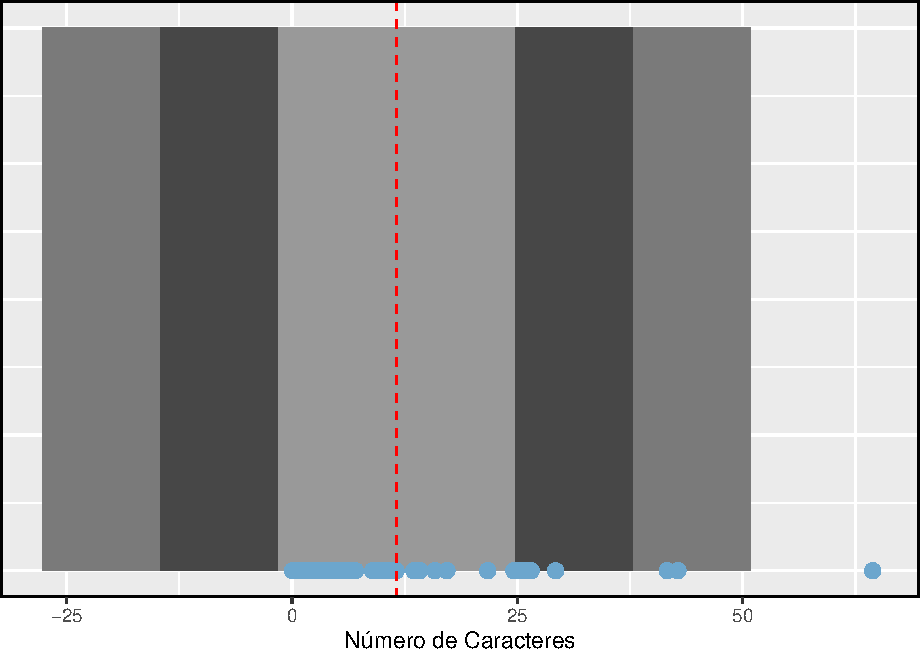
\includegraphics{_main_files/figure-latex/sdAsRuleForEmailNumChar-1.pdf}
\caption{\label{fig:sdAsRuleForEmailNumChar}No banco de dados num\_char, 41 dos 50 (82\%) emails estão dentro de 1 desvio padrão da média, e 47 dos 50 e-mails (94\%) estão dentro de 2 desvios padrão. Normalmente, cerca de 70\% dos dados estão dentro de 1 desvio padrão da média e 95\% estão dentro de 2 desvios padrão, embora essa regra regal seja menos precisa para dados distorcidos, conforme mostrado neste exemplo.}
\end{figure}

Desvio padrão descreve variabilidade: Concentre-se no significado conceitual do desvio padrão como um descritor de variabilidade em vez das fórmulas. Normalmente, 70\% dos dados estarão dentro de um desvio padrão da média e cerca de 95\% estarão dentro de dois desvios padrão. No entanto, como visto na Figura \ref{fig:sdAsRuleForEmailNumChar} e na Figura\ref{fig:severalDiffDistWithSdOf1}, estas percentagens não são regras restritas.

\begin{figure}
\centering
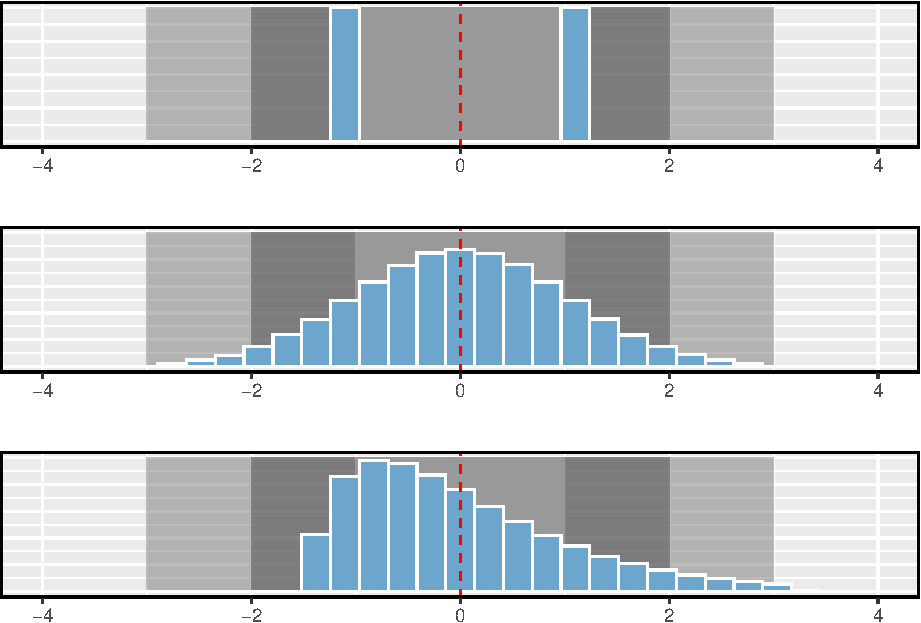
\includegraphics{_main_files/figure-latex/severalDiffDistWithSdOf1-1.pdf}
\caption{\label{fig:severalDiffDistWithSdOf1}Três distribuições populacionais muito diferentes com a mesma média (0) e desvio padrão (1)}
\end{figure}

\begin{center}\rule{0.5\linewidth}{0.5pt}\end{center}

\begin{exercise}
\protect\hypertarget{exr:unnamed-chunk-25}{}{\label{exr:unnamed-chunk-25} }O conceito de forma de uma distribuição foi introduzido. Uma boa descrição da forma de uma distribuição deve incluir a modalidade e se a distribuição é simétrica ou assimétrica para um lado. Usando a Figura \ref{fig:severalDiffDistWithSdOf1} por exemplo, explique por que tal descrição é importante\footnote{A Figura \ref{fig:severalDiffDistWithSdOf1} mostra três distribuições que parecem bem diferentes, mas todas têm a mesma média, variância e desvio padrão. Usando a modalidade, podemos distinguir entre o primeiro gráfico (bimodal) e os dois últimos (unimodal). Usando a assimetria, podemos distinguir entre o último plot (direita inclinada) e as duas primeiras. Enquanto uma imagem, como um histograma, conta uma história mais completa, podemos usar a modalidade e a forma (simetria / inclinação) para caracterizar informações básicas sobre uma distribuição.},
\end{exercise}

\begin{center}\rule{0.5\linewidth}{0.5pt}\end{center}

\begin{example}
\protect\hypertarget{exm:unnamed-chunk-26}{}{\label{exm:unnamed-chunk-26} }Descrever a distribuição da variável \texttt{num\_char} usando o histograma na Figura \ref{fig:email50NumCharHist}. A descrição deve incorporar o centro, a variabilidade e a forma da distribuição e também deve ser colocada no contexto: o número de caracteres nos emails. Observe também quaisquer casos especialmente incomuns.\}
\end{example}

A distribuição de contagens de caracteres de e-mails é unimodal e muito inclinada. Muitas das contagens se aproximam da média em 11.600, e a maioria cai dentro de um desvio padrão (13.130) da média. Há um e-mail excepcionalmente longo com cerca de 65.000 caracteres.

Na prática, a variância e o desvio padrão às vezes são usados como um meio para um fim, onde o ``fim'' é capaz de estimar com precisão a incerteza associada a uma estatística de amostra. Por exemplo, mais a frente usaremos a variância e o desvio padrão para avaliar quão próxima a média da amostra é da média populacional.

\hypertarget{boxplotQuantileMedian}{%
\subsection{Box-plot, quartis e a mediana}\label{boxplotQuantileMedian}}

O \textbf{box-plot} resume um conjunto de dados usando cinco estatísticas ao mesmo tempo em que grava observações incomuns. A Figura \ref{fig:boxPlotLayoutNumVar} fornece um gráfico de pontos vertical ao lado de um box-plot da variável \texttt{var\_char} do banco de dados \texttt{email50}.

\begin{figure}
\centering
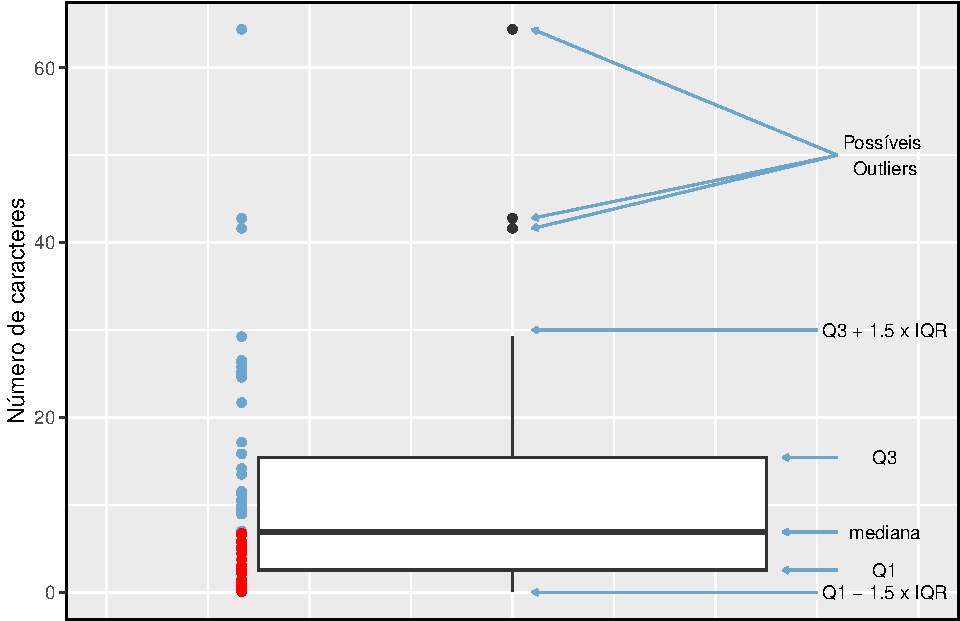
\includegraphics{_main_files/figure-latex/boxPlotLayoutNumVar-1.pdf}
\caption{\label{fig:boxPlotLayoutNumVar}Um gráfico de pontos vertical ao lado de uma caixa rotulada para o número de caracteres em 50 emails. A mediana (6.890) divide os dados em 50\% inferiores e os 50\% superiores, marcados no gráfico de pontos por traços horizontais e círculos abertos, respectivamente.}
\end{figure}

O primeiro passo na construção de um box-plot é desenhar uma linha escura indicando a \textbf{mediana}, que divide os dados ao meio. A Figura \ref{fig:boxPlotLayoutNumVar} mostra 50\% dos dados caindo abaixo da mediana pontos vermelhos) e outros 50\% caindo acima da mediana (pontos azuis). Existem 50 contagens de caracteres no conjunto de dados (um número par) para que os dados sejam perfeitamente divididos em dois grupos de 25. Nós tomamos a mediana, neste caso, como: \((\text{6.768} + \text{7.012}) / 2 = \text{6.890}\). Quando há um número ímpar de observações, haverá exatamente uma observação que divide os dados em duas metades e, nesse caso, a observação é a mediana (sem necessidade de média).

Mediana: o número no meio: Se os dados forem ordenados do menor para o maior, a \textbf{mediana} é a observação no meio. Se houver um número par de observações, haverá dois valores no meio e a mediana será considerada como média desses dois valores.

O segundo passo na construção de um box-plot é desenhar um retângulo para representar os 50\% do meio dos dados. O comprimento total da caixa, mostrado verticalmente na Figura \ref{fig:boxPlotLayoutNumVar}, é chamado de \textbf{intervalo interquartílico} (IQR). Isso, como o desvio padrão, é uma medida de variabilidade dos dados. Quanto mais variáveis os dados, maior o desvio padrão e o IQR. Os dois limites da caixa são chamados de primeiro quartil (Q1) (o 25 percentil, ou seja, 25\% dos dados ficam abaixo desse valor) e o terceiro quartil (Q3) (O 75 percentil, 75\% dos dados ficam abaixo desse valor), e estes são frequentemente rotulados \(Q_1\) e \(Q_3\), respectivamente.

Intervalo Interquartílico (IQR): O IQR é o comprimento da caixa em um box-plot. É calculado como

\begin{eqnarray*}
IQR = Q_3 - Q_1
\end{eqnarray*}
onde \(Q_1\) e \(Q_3\) são os 25 e 75 percentis.\}

\begin{center}\rule{0.5\linewidth}{0.5pt}\end{center}

\begin{exercise}
\protect\hypertarget{exr:unnamed-chunk-27}{}{\label{exr:unnamed-chunk-27} }Qual porcentagem dos dados está entre \(Q_1\) e a mediana? Qual porcentagem está entre a mediana e \(Q_3\)?\footnote{Como \(Q_1\) e \(Q_3\) capturam o meio 50\% dos dados e a mediana divide os dados no meio, 25\% dos dados ficam entre \(Q_1\) e a mediana e outros 25\% entre a mediana e \(Q_3\).}
\end{exercise}

\begin{center}\rule{0.5\linewidth}{0.5pt}\end{center}

Estendendo-se para fora da caixa, as linhas verticais tentam capturar os dados fora da caixa, no entanto, nunca é permitido que seu alcance seja superior a \(1.5\times IQR\)\footnote{Enquanto a escolha de exatamente 1.5 é arbitrária, é o valor mais comumente usado para box-plots.}. Eles capturam tudo dentro desse alcance. Na Figura \ref{fig:boxPlotLayoutNumVar}, a linha vertical superior não se estende até os últimos três pontos, o que está além de \(Q_3 + 1.5\times IQR\), e assim se estende apenas até o último ponto abaixo desse limite. A linha vertical inferior para no valor mais baixo, uma vez que não há dados adicionais para alcançar. O limite inferior não é mostrado na figura porque o gráfico não se estende até \(Q_1 - 1,5\times IQR\). Em certo sentido, a caixa é como o corpo da caixa e as linhas verticais são como seus braços tentando alcançar o resto dos dados.

Qualquer observação que esteja além dessas linhas verticais é rotulada com um ponto. O objetivo de rotular esses pontos - em vez de apenas estender as linhas aos valores mínimo e máximo observados - é ajudar a identificar quaisquer observações que pareçam estar distantes do resto dos dados. Observações anormalmente distantes são chamadas de \textbf{outliers}. Nesse caso, seria razoável classificar os e-mails com contagens de caracteres de 41.623, 42.793 e 64.401 como outliers, uma vez que estão numericamente distantes da maioria dos dados.

Outliers são extremos: Um \textbf{outlier} é uma observação que parece extrema em relação ao resto dos dados.

Por que é importante procurar outliers: O exame de dados para possíveis outliers serve a muitos propósitos úteis, incluindo:

\begin{itemize}
\item
  Identificando forte inclinação na distribuição.
\item
  Identificar na coleta de dados erros de entrada. Por exemplo, reexaminamos o email supostamente com 64.401 caracteres para garantir que esse valor é preciso.
\item
  Fornecendo informações sobre propriedades interessantes dos dados.
\end{itemize}

\begin{center}\rule{0.5\linewidth}{0.5pt}\end{center}

\begin{exercise}
\protect\hypertarget{exr:unnamed-chunk-28}{}{\label{exr:unnamed-chunk-28} }A observação 64.401, suspeita de ser um outlier, foi uma observação precisa. O que tal observação sugere sobre a natureza do caráter nos e-mails?\footnote{Que ocasionalmente pode haver e-mails muito longos.}
\end{exercise}

\begin{center}\rule{0.5\linewidth}{0.5pt}\end{center}

\begin{center}\rule{0.5\linewidth}{0.5pt}\end{center}

\begin{exercise}
\protect\hypertarget{exr:unnamed-chunk-29}{}{\label{exr:unnamed-chunk-29} }Usando a Figura \ref{fig:boxPlotLayoutNumVar}, estime os seguintes valores para a variável número de caracteres nos dados \texttt{email50}: (a) \(Q_1\), (b) \(Q_3\), e (c) IQR.\footnote{Essas estimativas visuais variam um pouco de uma pessoa para outra: \(Q_1=\) 3,000, \(Q_3=\) 15,000, \$\text{IQR}=Q\_3 - Q\_1 = \$ 12,000. (Os verdadeiros valores: \(Q_1=\) 2,536, \(Q_3=\) 15,411, \$\text{IQR} = \$ 12,875.)}
\end{exercise}

\begin{center}\rule{0.5\linewidth}{0.5pt}\end{center}

\hypertarget{statisticsRobust}{%
\subsection{Estatísticas robustas}\label{statisticsRobust}}

Como as estatísticas da amostra do conjunto de dados \texttt{num\_char} são afetados pela observação 64.401? O que teria acontecido se este email não fosse observado? O que aconteceria com estas estatísticas se a observação 64.401 fosse ainda maior, digamos 150.000? Esses cenários são plotados ao lado dos dados originais na Figura \ref{fig:email50NumCharDotPlotRobustEx}, e estatísticas de amostra são computadas em cada cenário na Tabela \ref{tab:robustOrNotTable}.

\begin{figure}
\centering
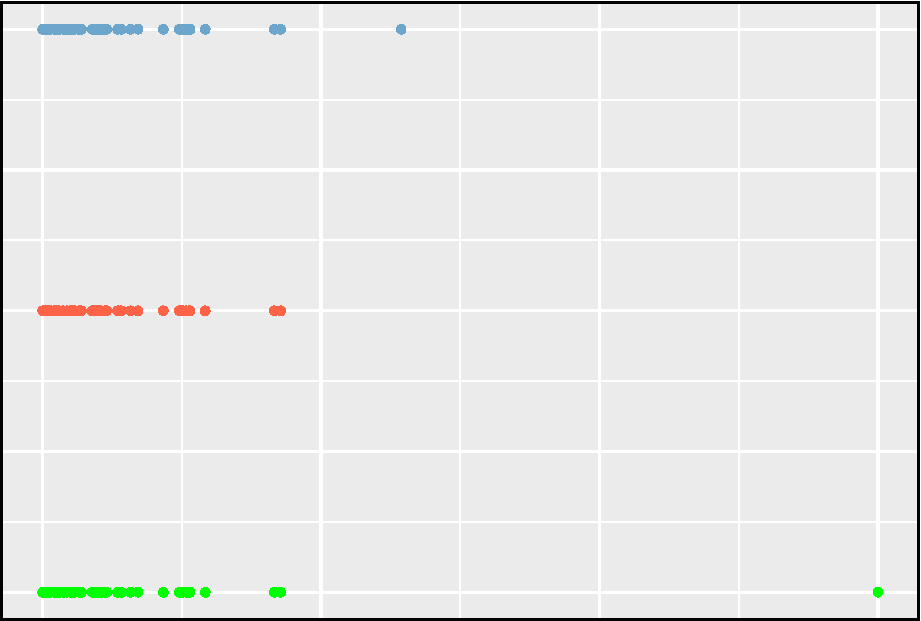
\includegraphics{_main_files/figure-latex/email50NumCharDotPlotRobustEx-1.pdf}
\caption{\label{fig:email50NumCharDotPlotRobustEx}Gráficos de pontos dos dados de contagem de caracteres originais e dois conjuntos de dados modificados.}
\end{figure}

\begin{table}

\caption{\label{tab:robustOrNotTable}Uma comparação de como a mediana, IQR, média, e desvio padrão muda quando observações extremas estiverem presentes.}
\centering
\begin{tabular}[t]{l|c|c|c|c}
\hline
  & Mediana & IQR & Média & Desvio Padrão\\
\hline
Original (Azul) & 6.8895 & 12.87525 & 11.59822 & 13.12526\\
\hline
Sem o dado 64.401 (Vermelho) & 6.7680 & 11.70200 & 10.52061 & 10.79768\\
\hline
150.000 no lugar de 64.401 (Verde) & 6.8895 & 12.87525 & 13.31020 & 22.43436\\
\hline
\end{tabular}
\end{table}

\begin{center}\rule{0.5\linewidth}{0.5pt}\end{center}

\begin{exercise}
\protect\hypertarget{exr:numCharWhichIsMoreRobust}{}{\label{exr:numCharWhichIsMoreRobust} }(a) Qual é mais afetado por observações extremas, a média ou mediana? A Tabela \ref{tab:robustOrNotTable} pode ser útil.
(b) O desvio padrão ou IQR é mais afetado por observações extremas?\footnote{(a) A média é mais afetada. (b) O desvio padrão é mais afetado. Explicações completas são fornecidas no material a seguir à Prática Orientada \ref{exr:numCharWhichIsMoreRobust}.}
\end{exercise}

\begin{center}\rule{0.5\linewidth}{0.5pt}\end{center}

A mediana e o IQR são chamados de \textbf{estimativas robustas} porque observações extremas têm pouco efeito sobre seus valores. A média e o desvio padrão são muito mais afetados pelas mudanças nas observações extremas.

\begin{example}
\protect\hypertarget{exm:unnamed-chunk-30}{}{\label{exm:unnamed-chunk-30} }A mediana e o IQR não mudam muito sob os três cenários na Tabela \ref{tab:robustOrNotTable}. Por que isso pode acontecer?
\end{example}

A mediana e o IQR são sensíveis apenas a números próximos de \(Q_1\), a mediana e \(Q_3\). Como os valores nessas regiões são relativamente estáveis - não há grandes saltos entre as observações - a mediana e as estimativas de IQR também são bastante estáveis.

\begin{center}\rule{0.5\linewidth}{0.5pt}\end{center}

\begin{exercise}
\protect\hypertarget{exr:unnamed-chunk-31}{}{\label{exr:unnamed-chunk-31} }A distribuição dos preços dos veículos tende a ser bem distorcida, com alguns carros de luxo e esportivos pendurados na cauda direita. Se você estava procurando por um carro novo e se preocupava com o preço, deveria estar mais interessado no preço médio ou mediano dos veículos vendidos, supondo que você esteja no mercado para um carro comum? \footnote{Compradores de um `carro comum' devem estar preocupados com o preço médio. As vendas de carros de luxo podem inflacionar drasticamente o preço médio, enquanto a mediana será mais robusta em relação à influência dessas vendas.}
\end{exercise}

\begin{center}\rule{0.5\linewidth}{0.5pt}\end{center}

\hypertarget{transformingDataSubsection}{%
\subsection{Transformando dados (tópico especial)}\label{transformingDataSubsection}}

Quando os dados são muito distorcidos, as vezes os transformamos para que sejam mais fáceis de modelar. Considere o histograma dos salários dos jogadores de beisebol da Major League de 2010, que é mostrado na Figura \ref{fig:histMLBSalariesReg}.

\begin{figure}
\centering
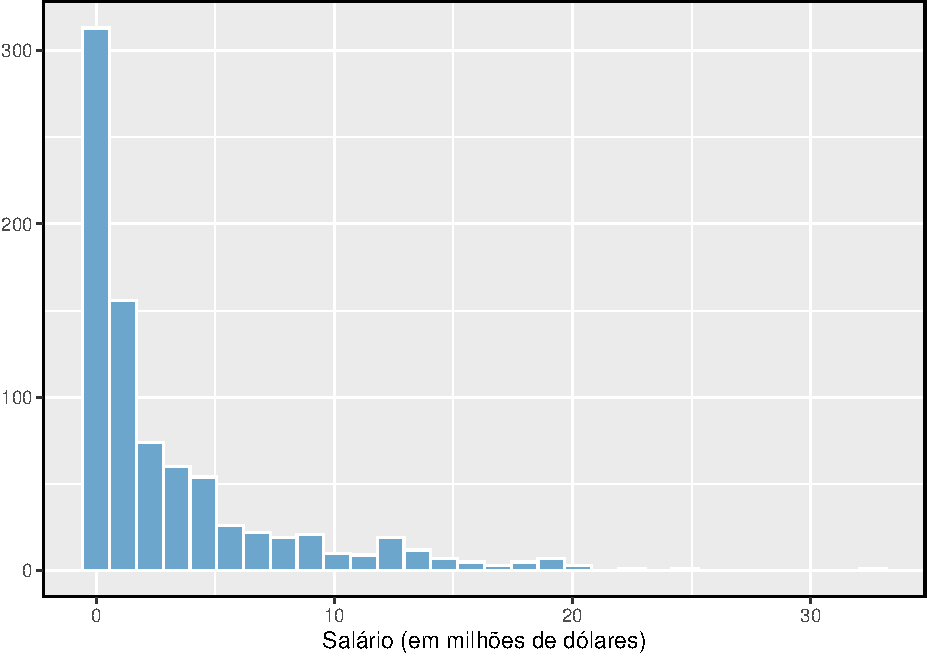
\includegraphics{_main_files/figure-latex/histMLBSalariesReg-1.pdf}
\caption{\label{fig:histMLBSalariesReg}Histograma dos salários dos jogadores da MLB em 2010, em milhões de dólares}
\end{figure}

\begin{figure}
\centering
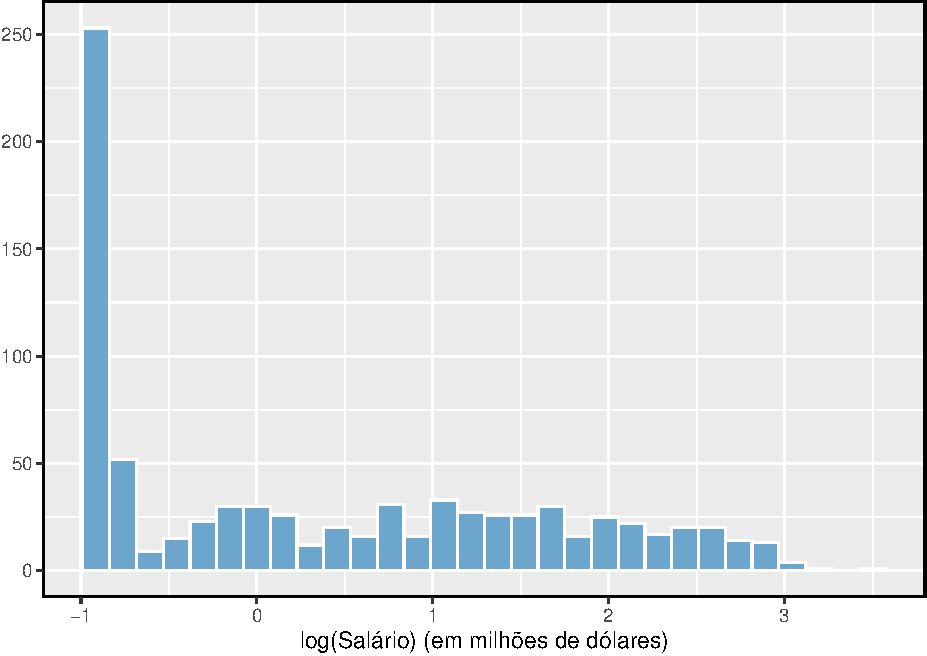
\includegraphics{_main_files/figure-latex/histMLBSalariesLog-1.pdf}
\caption{\label{fig:histMLBSalariesLog}Histograma dos salários dos jogadores da MLB transformados em log para 2010.}
\end{figure}

\begin{example}
\protect\hypertarget{exm:unnamed-chunk-32}{}{\label{exm:unnamed-chunk-32} }O histograma dos salários dos jogadores da MLB é útil, pois podemos ver que os dados são extremamente distorcidos e centrado (medido pela mediana) em cerca de \$1 milhão. O que não é útil sobre este gráfico?\}
\end{example}

A maioria dos dados é coletada em um compartimento no histograma e os dados são tão distorcidos que muitos detalhes nos dados são obscurecidos.

Existem algumas transformações padrão que são geralmente aplicadas quando grande parte do cluster de dados está próximo de zero (em relação aos valores maiores no conjunto de dados) e todas as observações são positivas. A \textbf{transformação} é um reescalonamento dos dados usando uma função. Por exemplo, uma plotagem do logaritmo natural\footnote{Estatísticos geralmente escrevem o logaritmo natural como \(\log\). Você pode estar mais familiarizado com isso sendo escrito como \(\ln\).} dos salários dos jogadores resulta em um novo histograma na Figura \ref{fig:histMLBSalariesLog}. Às vezes, é mais fácil trabalhar com dados transformados ao aplicar modelos estatísticos, pois os dados transformados são muito menos distorcidos e os outliers são geralmente menos extremos.

Transformações também podem ser aplicadas a uma ou ambas as variáveis em um gráfico de dispersão. Um gráfico de dispersão das variáveis \texttt{quebra\_linha} e \texttt{num\_char} é mostrado na Figura \ref{fig:email50LinesCharactersMod}, que foi mostrado anteriormente na Figura \ref{fig:email50LinesCharacters}. Podemos ver uma associação positiva entre as variáveis e que muitas observações são agrupadas perto de zero. Mais a frente podemos querer usar uma linha reta para modelar os dados. No entanto, descobriremos que os dados em seu estado atual não podem ser modelados muito bem.

\begin{figure}
\centering
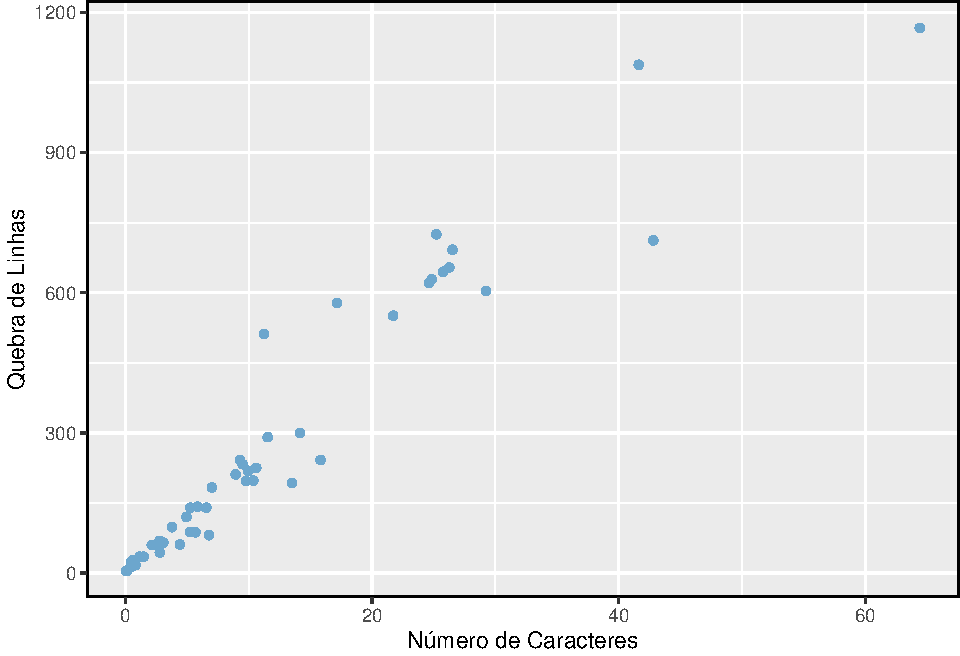
\includegraphics{_main_files/figure-latex/email50LinesCharactersMod-1.pdf}
\caption{\label{fig:email50LinesCharactersMod}Gráfico de dispersão de quebra de linha contra número de caracteres para 50 emails}
\end{figure}

A Figura \ref{fig:email50LinesCharactersModLog} mostra um gráfico de dispersão onde ambas variáveis foram transformadas usando uma transformação log (base \(e\)). Embora haja uma associação positiva em cada parcela, os dados transformados mostram uma tendência mais estável, que é mais fácil de modelar do que os dados não transformados.

\begin{figure}
\centering
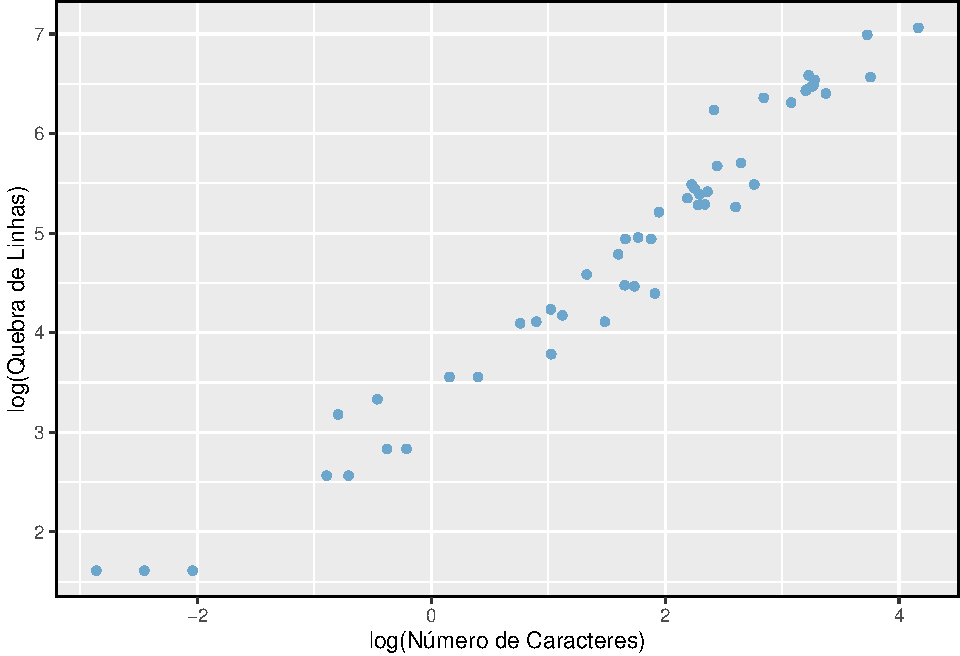
\includegraphics{_main_files/figure-latex/email50LinesCharactersModLog-1.pdf}
\caption{\label{fig:email50LinesCharactersModLog}Um gráfico de dispersão dos mesmos dados, mas em que cada variável foi transformada em log.}
\end{figure}

Transformações além do logaritmo podem ser úteis também. Por exemplo, a raiz quadrada (\(\sqrt{\text{observação original}}\)) e inversa (\(\frac{1}{\text{observação original}}\)) são usados por estatísticos. Os objetivos comuns na transformação de dados são ver a estrutura de dados de maneira diferente, reduzir a distorção, auxiliar na modelagem ou endireitar um relacionamento não linear em um gráfico de dispersão.

\hypertarget{mapingDataSubsection}{%
\subsection{Mapeamento de dados (tópico especial)\}}\label{mapingDataSubsection}}

O banco de dados \texttt{condado} oferece muitas variáveis numéricas que poderíamos plotar usando gráficos de pontos, gráficos de dispersão ou box-plots, mas eles perdem a verdadeira natureza dos dados. Em vez disso, quando nos deparamos com dados
geográficos, devemos mapeá-lo usando um \textbf{mapa de intensidade}, onde as cores são usadas para mostrar valores mais altos e maisbaixos de uma variável. As Figuras \ref{fig:countyIntensityMaps1}, \ref{fig:countyIntensityMaps2}, \ref{fig:countyIntensityMaps3} e \ref{fig:countyIntensityMaps4} mostram mapas de intensidade para gastos federais per capita (\texttt{var\_fed}), taxa de pobreza em porcentagem (\texttt{poverty}), taxa de casa própria em porcentagem (\texttt{homeownership}), e renda familiar mediana (\texttt{med\_income}). A paleta colorida indica quais cores correspondem a
quais valores. Observe que os mapas de intensidade geralmente não são muito úteis para obter valores precisos em nenhum estado, mas são muito úteis para ver tendências geográficas e gerar interessantes perguntas de pesquisa.

\begin{figure}
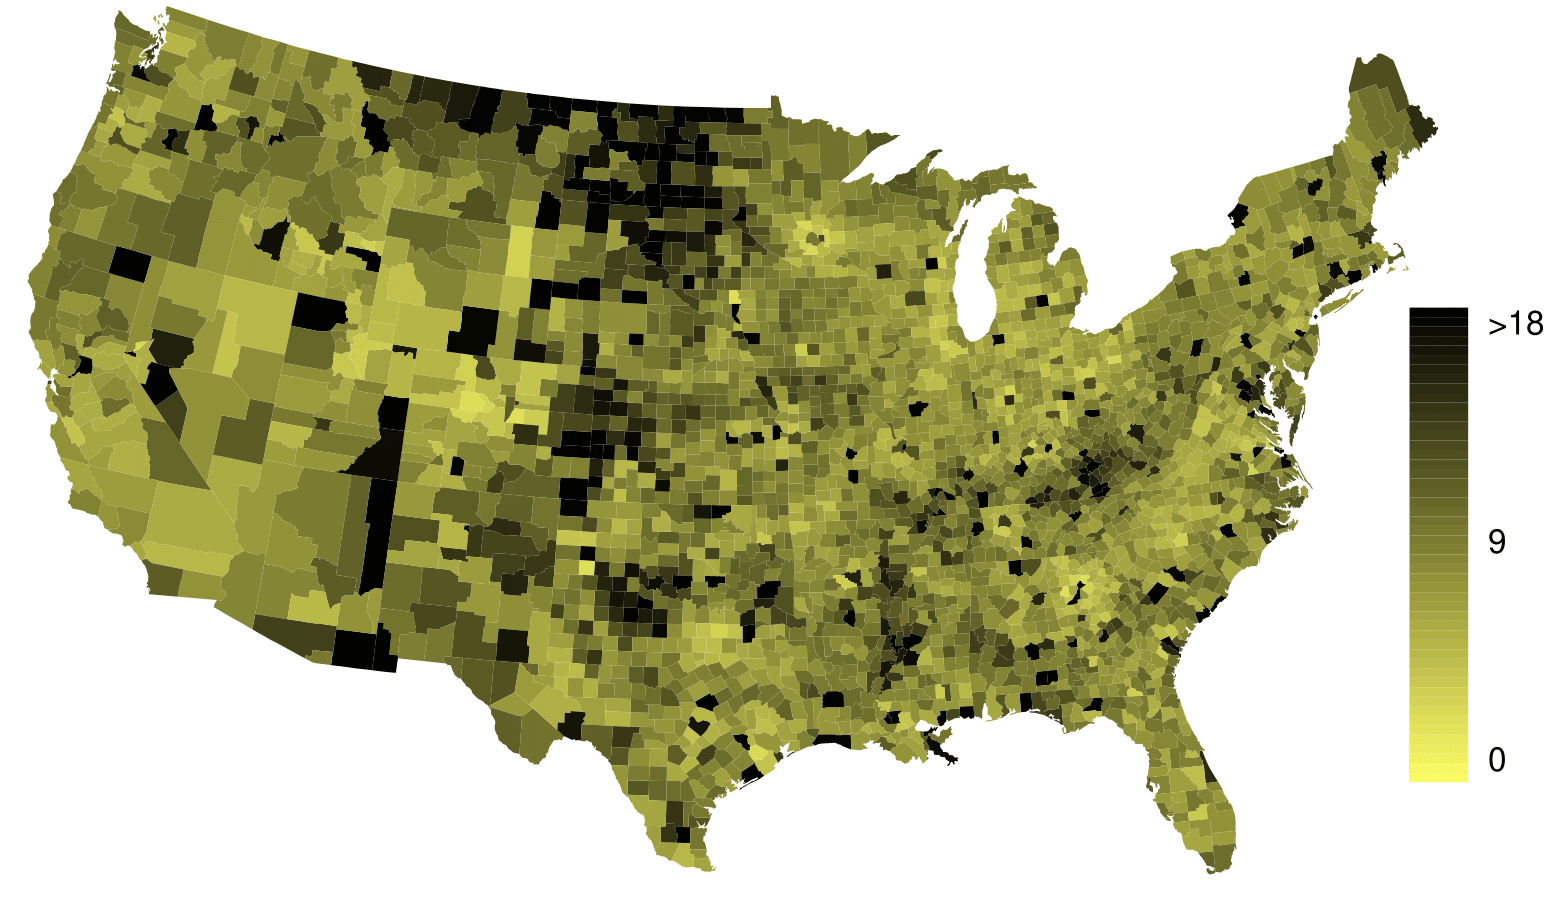
\includegraphics[width=0.5\linewidth]{images/c1/countyFedSpendMap} \caption{Mapa dos gastos federais (dólares per capita)}\label{fig:countyIntensityMaps1}
\end{figure}

\begin{figure}
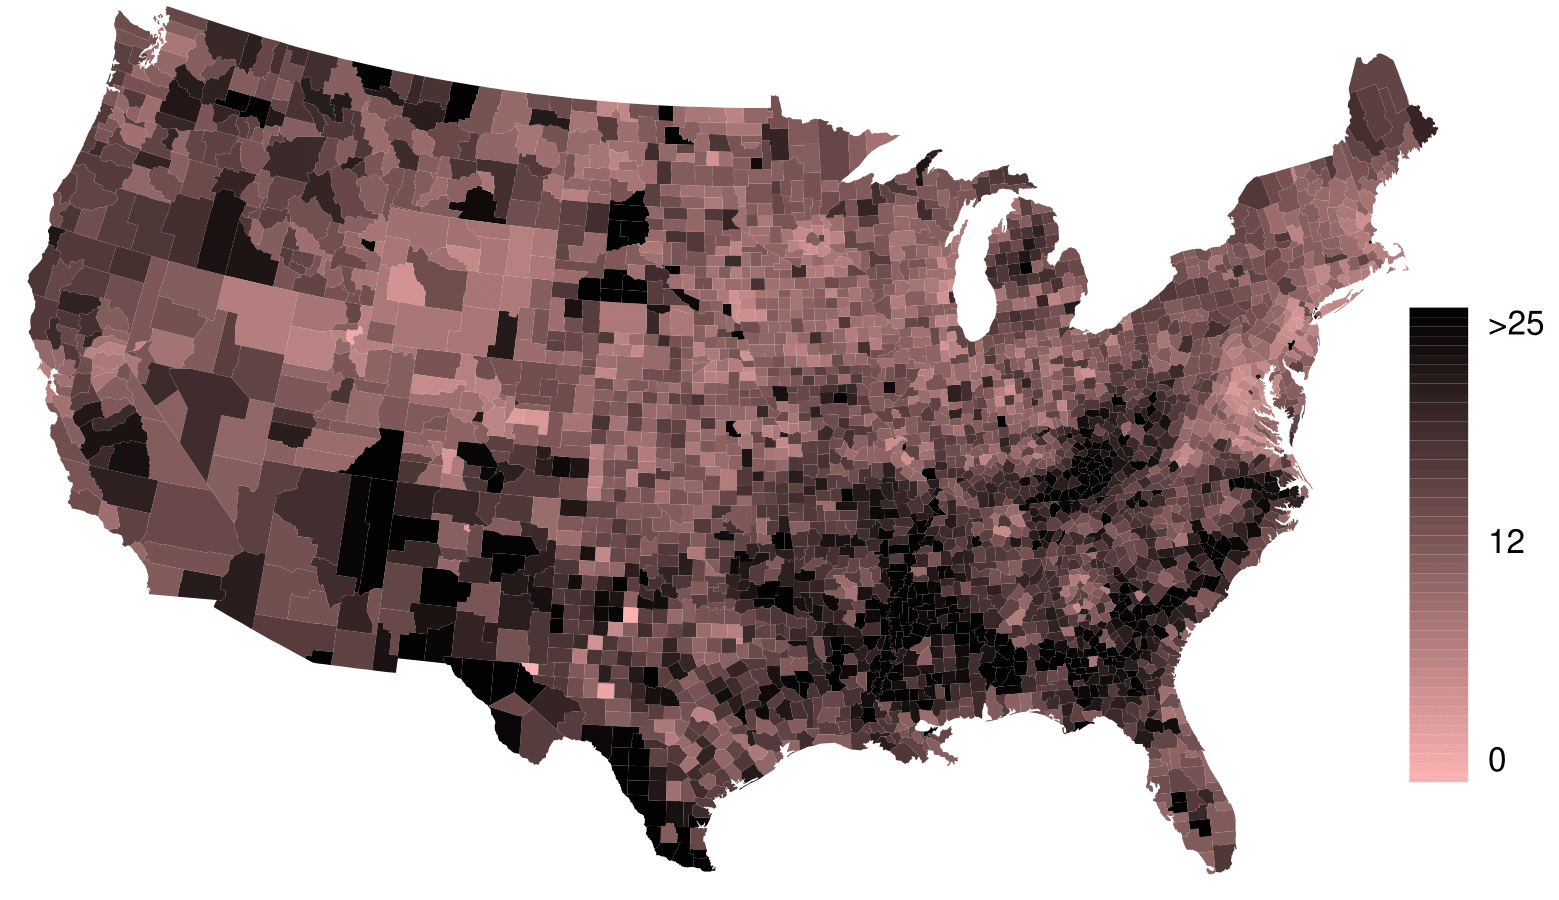
\includegraphics[width=0.5\linewidth]{images/c1/countyPovertyMap} \caption{Mapa de intensidade da taxa de pobreza (por cento).}\label{fig:countyIntensityMaps2}
\end{figure}

\begin{figure}
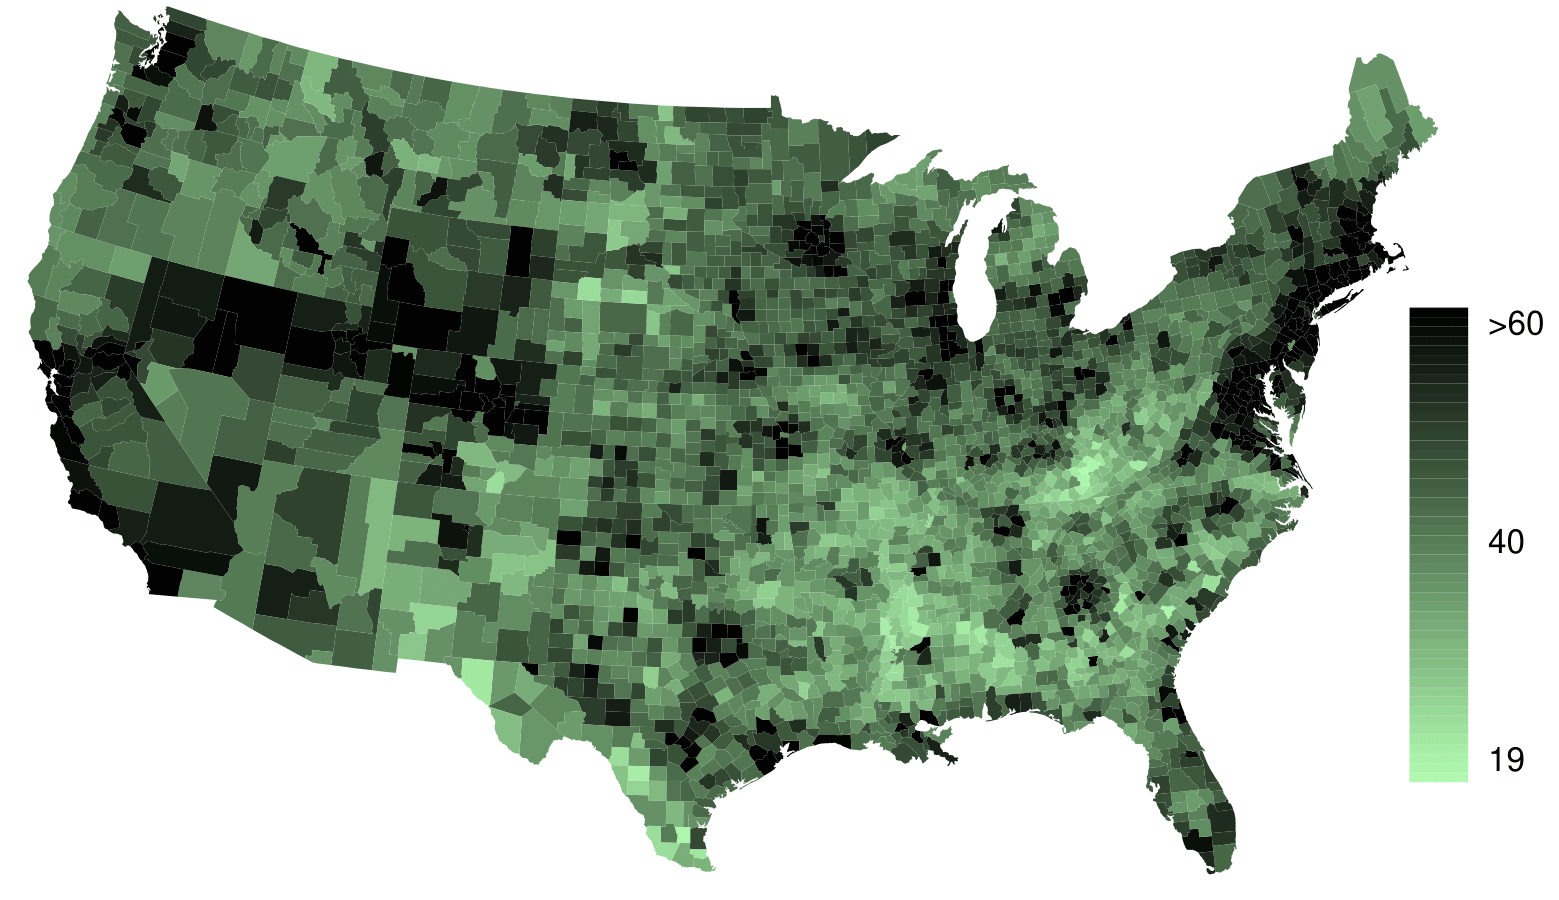
\includegraphics[width=0.5\linewidth]{images/c1/countyMedIncomeMap} \caption{Mapa de intensidade da taxa de propriedade (por cento).}\label{fig:countyIntensityMaps3}
\end{figure}

\begin{figure}
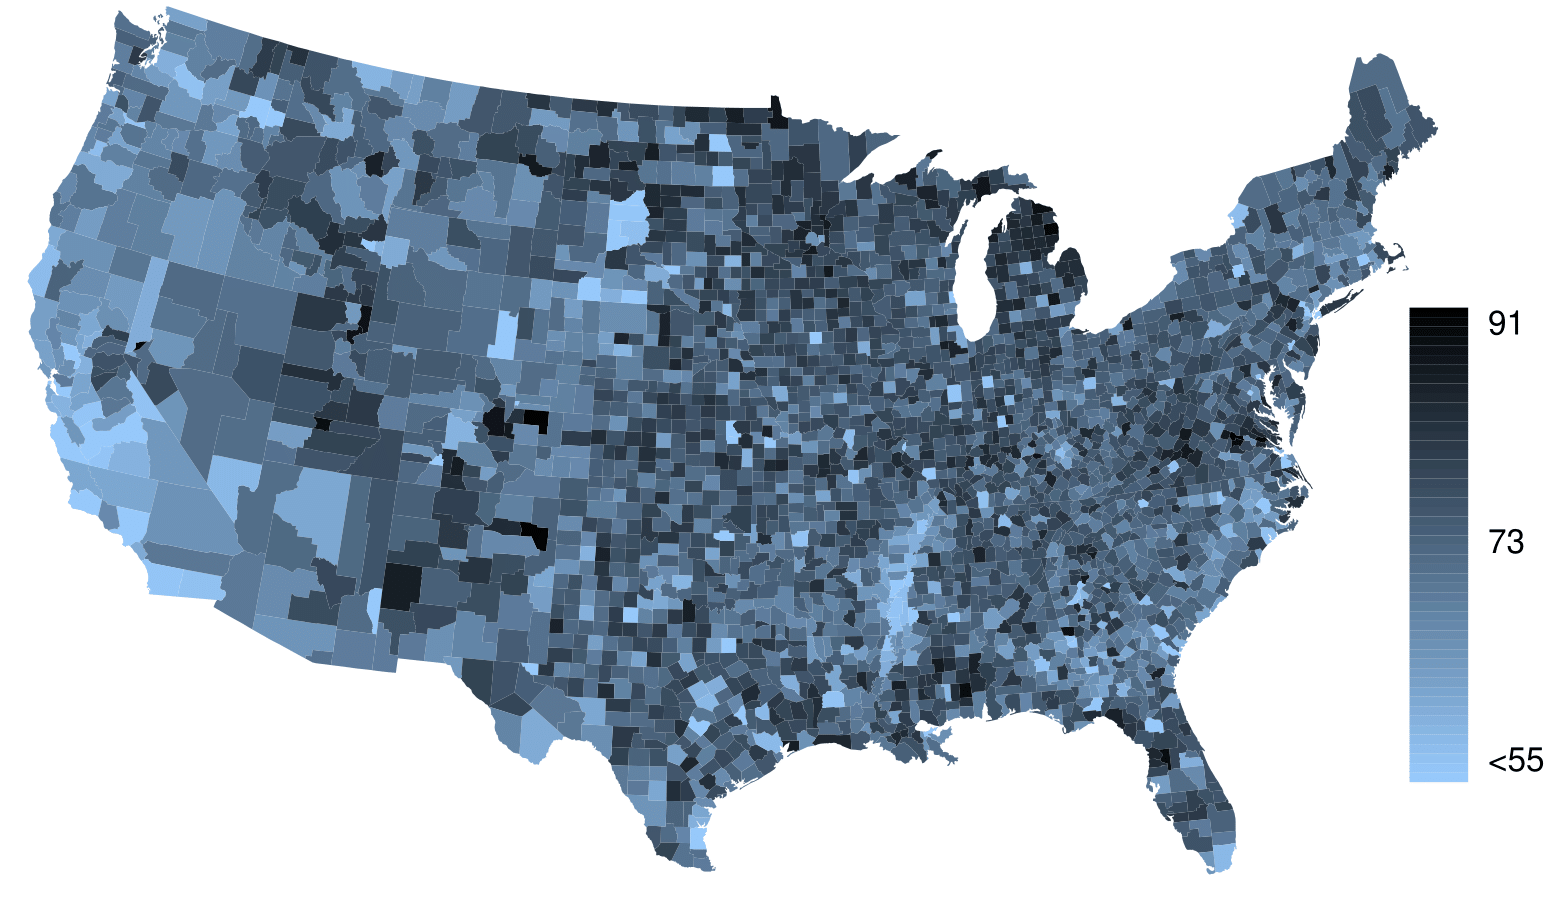
\includegraphics[width=0.5\linewidth]{images/c1/countyHomeownershipMap} \caption{Mapa de intensidade da renda familiar média (1000 dólares).}\label{fig:countyIntensityMaps4}
\end{figure}

\begin{example}
\protect\hypertarget{exm:unnamed-chunk-33}{}{\label{exm:unnamed-chunk-33} }Que características interessantes são evidentes nos mapas de intensidade de gasto e pobreza?\}
\end{example}

O mapa de intensidade de gasto federal mostra gastos substanciais nas Dakotas e ao longo da parte central a oeste da fronteira canadense, o que pode estar relacionado ao boom do petróleo nesta região. Há várias outras parcelas de gastos federais, como uma faixa vertical no leste de Utah e Arizona e a área onde o Colorado, Nebraska e Kansas se encontram. Há também condados aparentemente aleatórios com gastos federais muito altos em relação aos seus vizinhos. Se não limitássemos o gasto federal em \$18 per capita, descobriríamos que alguns municípios têm gastos federais extremamente altos, enquanto quase não há gastos federais nos municípios vizinhos. Esses municípios de alto gasto podem conter bases militares, empresas com grandes contratos governamentais ou outras instalações governamentais com muitos funcionários.

As taxas de pobreza são evidentemente mais altas em alguns locais. Notavelmente, o sul mostra taxas de pobreza mais altas, assim como a fronteira sudoeste do Texas. A faixa vertical do leste de Utah e do Arizona, mencionada acima por seus gastos federais mais altos, também parece ter taxas mais altas de pobreza (embora geralmente seja observada pouca relação entre as duas variáveis). Altos índices de pobreza são evidentes nas planícies aluviais do Mississipi, um pouco ao norte de Nova Orleans e também em uma grande parte de Kentucky e West Virginia.

\begin{center}\rule{0.5\linewidth}{0.5pt}\end{center}

\begin{exercise}
\protect\hypertarget{exr:unnamed-chunk-34}{}{\label{exr:unnamed-chunk-34} }Que características interessantes são evidentes no mapa de intensidade na Figura \ref{fig:countyIntensityMaps3}?\footnote{Nota: as respostas irão variar. Há uma correspondência muito forte entre as áreas de alta renda e metropolitana. Você pode procurar por cidades grandes com as quais esteja familiarizado e tentar localizá-las no mapa como pontos escuros.}
\end{exercise}

\begin{center}\rule{0.5\linewidth}{0.5pt}\end{center}

\hypertarget{categoricalData}{%
\section{Considerando dados categóricos}\label{categoricalData}}

Como os dados numéricos, os dados categóricos também podem ser organizados e analisados. Nesta seção, apresentaremos tabelas e outras ferramentas básicas para dados categóricos que são usadas neste livro. O conjunto de dados \texttt{email50} representa uma amostra de um conjunto de dados de e-mail maior chamado \texttt{email}. Este conjunto de dados maior contém informações sobre 3.921 e-mails. Nesta seção, examinaremos se a presença de números, pequenos ou grandes, em um e-mail fornece qualquer valor útil na classificação de e-mail como spam ou não spam.

\hypertarget{tablesBarGraphics}{%
\subsection{Tabelas de Contingência e Gráficos de Barras}\label{tablesBarGraphics}}

A Tabela \ref{tab:emailSpamNumberTableTotals} resume duas variáveis: \texttt{spam} e \texttt{número}. Lembre-se de que \texttt{número} é uma variável categórica que descreve se um email não contém números, apenas números pequenos (valores abaixo de 1 milhão) ou pelo menos um número grande (um valor de 1 milhão ou mais). Uma tabela que resume dados para duas variáveis categóricas dessa maneira é chamada de \textbf{tabela de contingência}. Cada valor na tabela representa o número de vezes que uma combinação específica de resultados de variáveis ocorreu. Por exemplo, o valor 149 corresponde ao número de e-mails no conjunto de dados que são spam e não tinham nenhum número listado no e-mail. Os totais de linha e coluna também estão incluídos. O termo \textbf{totais da linha} fornece as contagens totais em cada linha (por ex.\(149 + 168 + 50 = 367\)), e os \textbf{totais da coluna} são totais contagens abaixo de cada coluna.

Uma tabela para uma única variável é chamada de \textbf{tabela de frequência}. A Tabela \ref{tab:emailNumberTable} é uma tabela de frequência para a variável \texttt{número}. Se substituíssemos as contagens por porcentagens ou proporções, a tabela seria chamada de \textbf{tabela de frequência relativa}.

\begin{table}

\caption{\label{tab:emailSpamNumberTableTotals}Uma tabela de contingência para spam e número.}
\centering
\begin{tabular}[t]{l|c|c|c|c}
\hline
  & Nenhum & Pequeno & Grande & Total\\
\hline
Não Spam & 400 & 2659 & 495 & 3554\\
\hline
Spam & 149 & 168 & 50 & 367\\
\hline
Total & 549 & 2827 & 545 & 3921\\
\hline
\end{tabular}
\end{table}

\begin{table}

\caption{\label{tab:emailNumberTable}Uma tabela de frequências para a variável número}
\centering
\begin{tabular}[t]{c|c|c|c}
\hline
Nenhum & Pequeno & Grande & Total\\
\hline
549 & 2827 & 545 & 3921\\
\hline
\end{tabular}
\end{table}

Um gráfico de barras é uma maneira comum de exibir uma única variável categórica. O painel esquerdo da Figura \ref{fig:emailNumberBarPlot} mostra um \textbf{gráfico de barras} para a variável \textbf{número}. No gráfico da direita, as contagens são convertidas em proporções (por ex. \(549/3921=0.140\) para nenhum), mostrando a proporção de observações que estão em cada nível (ou seja, em cada categoria).

\begin{figure}
\centering
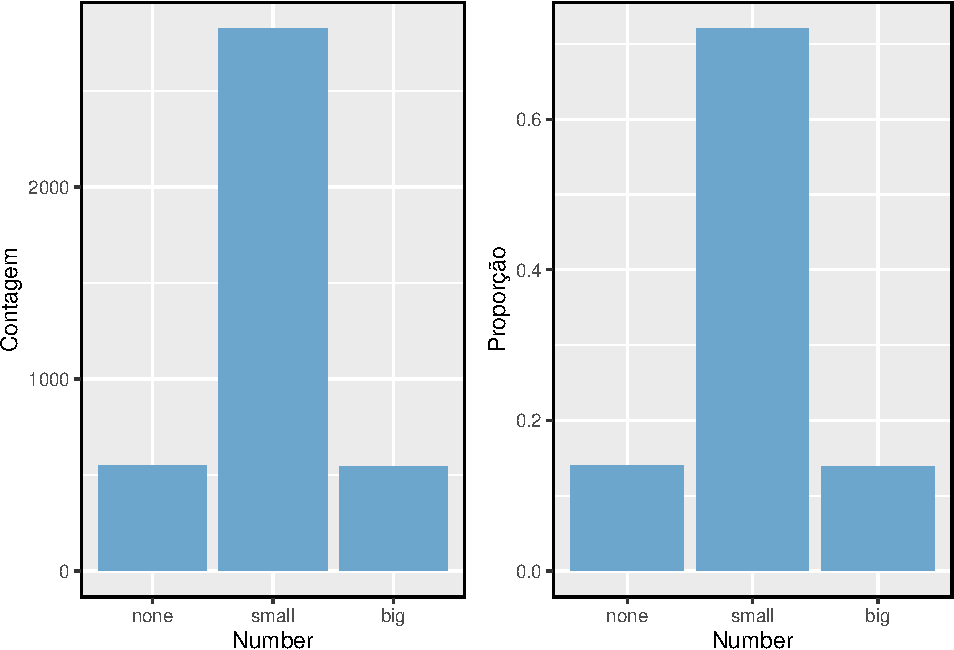
\includegraphics{_main_files/figure-latex/emailNumberBarPlot-1.pdf}
\caption{\label{fig:emailNumberBarPlot}Dois gráficos de barras para a variável número. O gráfico da esquerda mostra as contagens e o gráfico da direita mostra as proporções em cada grupo.}
\end{figure}

\hypertarget{rowColumnProportion}{%
\subsection{Proporções de linha e coluna}\label{rowColumnProportion}}

A Tabela \ref{tab:rowPropSpamNumber} mostra as proporções de linha para a Tabela \ref{tab:emailSpamNumberTableTotals}. As \textbf{proporções de linha} são computadas como as contagens divididas por seus totais de linha. O valor 149 na interseção de \texttt{spam} e \texttt{nenhum} é substituído por \(149/367=0.406\), isto é, 149 dividido por seu total de linhas, 367. Então, o que 0.406 representa? Corresponde à proporção de e-mails de spam na amostra que não inclui números na mensagem.

\begin{table}

\caption{\label{tab:rowPropSpamNumber}Uma tabela de contingência com proporções de linha para as variáveis spam e número}
\centering
\begin{tabular}[t]{l|c|c|c|c}
\hline
  & Nenhum & Pequeno & Grande & Total\\
\hline
Não Spam & 0.113 & 0.748 & 0.139 & 1\\
\hline
Spam & 0.406 & 0.458 & 0.136 & 1\\
\hline
Total & 0.140 & 0.721 & 0.139 & 1\\
\hline
\end{tabular}
\end{table}

Uma tabela de contingência das proporções da coluna é calculada de forma semelhante, onde cada \textbf{proporção da coluna} é calculada como a contagem dividida pelo total da coluna correspondente. A Tabela \ref{tab:colPropSpamNumber} mostra tal tabela, e aqui o valor 0.271 indica que 27,1\% de emails sem números eram spam. Essa taxa de spam é muito maior em comparação a e-mails com apenas números pequenos (5,9\%) ou grandes números (9,2\%). Porque essas taxas de spam variam entre os três níveis de \texttt{número} (nenhum, pequeno, grande), isso fornece evidências de que as variáveis \texttt{spam} e \texttt{número} estão associadas.

\begin{table}

\caption{\label{tab:colPropSpamNumber}Uma tabela de contingência com proporções de coluna para as variáveis spam e número}
\centering
\begin{tabular}[t]{l|c|c|c|c}
\hline
  & Nenhum & Pequeno & Grande & Total\\
\hline
Não Spam & 0.729 & 0.941 & 0.908 & 0.906\\
\hline
Spam & 0.271 & 0.059 & 0.092 & 0.094\\
\hline
Total & 1.000 & 1.000 & 1.000 & 1.000\\
\hline
\end{tabular}
\end{table}

Também poderíamos ter verificado uma associação entre \texttt{spam} e \texttt{número} na Tabela \ref{tab:rowPropSpamNumber} usando proporção de colunas. Ao comparar essas proporções de linha, analisamos as colunas para ver se a fração de emails sem números, números pequenos e números grandes variava de \texttt{spam} à \texttt{não\textasciitilde{}spam}.

\begin{center}\rule{0.5\linewidth}{0.5pt}\end{center}

\begin{exercise}
\protect\hypertarget{exr:unnamed-chunk-35}{}{\label{exr:unnamed-chunk-35} }O que 0,458 representa na Tabela \ref{tab:rowPropSpamNumber}? O que 0,059 representa na Tabela \ref{tab:colPropSpamNumber}?\footnote{0,458 representa a proporção de e-mails de spam que tinham um pequeno número. 0,059 representa a fração de e-mails com números pequenos que são spam.}
\end{exercise}

\begin{center}\rule{0.5\linewidth}{0.5pt}\end{center}

\begin{center}\rule{0.5\linewidth}{0.5pt}\end{center}

\begin{exercise}
\protect\hypertarget{exr:unnamed-chunk-36}{}{\label{exr:unnamed-chunk-36} }O que 0.139 representa na interseção de não spam e grande na Tabela \ref{tab:rowPropSpamNumber}? O que 0,908 representa na Tabela \ref{tab:colPropSpamNumber}?\footnote{0,139 representa a fração de e-mail não-spam que teve um grande número. 0,908 representa a fração de e-mails com números grandes que são e-mails não-spam.}
\end{exercise}

\begin{center}\rule{0.5\linewidth}{0.5pt}\end{center}

\begin{example}
\protect\hypertarget{exm:weighingRowColumnProportions}{}{\label{exm:weighingRowColumnProportions} }Os cientistas de dados usam estatísticas para filtrar o spam de mensagens de e-mail recebidas. Ao observar características específicas de um email, um cientista de dados pode classificar alguns emails como spam ou não como spam com alta precisão. Uma dessas características é se o email não contém números, números pequenos ou números grandes. Outra característica é se um email tem ou não algum conteúdo HTML. Uma tabela de contingência para as variáveis \texttt{spam} e \texttt{format} do conjunto de dados \texttt{email} são mostrados na Tabela \ref{tab:emailSpamHTMLTableTotals}. Lembre-se de que um email em HTML é um email com capacidade para formatação especial, por ex. texto em negrito. Na Tabela \ref{tab:emailSpamHTMLTableTotals}, qual seria mais útil para alguém que espera classificar email como spam ou email regular: proporções de linha ou coluna?
\end{example}

Essa pessoa estaria interessada em saber como a proporção de spam é alterada em cada formato de email. Isso corresponde a proporções de coluna: a proporção de spam em emails de texto sem formatação e a proporção de spam em emails HTML.

Se gerarmos as proporções da coluna, poderemos ver que uma fração maior de e-mails de texto sem formatação é spam (\(209/1195 = 17.5\%\)) do que em comparação com e-mails em HTML (\(158/2726 = 5.8\%\)). Esta informação por si só é insuficiente para classificar um email como spam ou não spam, pois mais de 80\% dos emails com texto simples não são spam. No entanto, quando combinamos cuidadosamente essas informações com muitas outras características, como \texttt{número} e outras variáveis, temos uma chance razoável de sermos capazes de classificar alguns e-mails como spam ou não spam.

\begin{table}

\caption{\label{tab:emailSpamHTMLTableTotals}Uma tabela de contingência para spam e format.}
\centering
\begin{tabular}[t]{l|c|c|c}
\hline
  & texto & HTML & Total\\
\hline
Não Spam & 986 & 2568 & 3554\\
\hline
Spam & 209 & 158 & 367\\
\hline
Total & 1195 & 2726 & 3921\\
\hline
\end{tabular}
\end{table}

O Exemplo \ref{exm:weighingRowColumnProportions} aponta que as proporções de linha e coluna não são equivalentes. Antes de escolher um formulário para uma tabela, é importante considerar cada um para garantir que a tabela mais útil seja construída.

\begin{center}\rule{0.5\linewidth}{0.5pt}\end{center}

\begin{exercise}
\protect\hypertarget{exr:unnamed-chunk-37}{}{\label{exr:unnamed-chunk-37} }Olhe para as Tabelas \ref{tab:rowPropSpamNumber} e \ref{tab:colPropSpamNumber}. O que seria mais útil para alguém na esperança de identificar e-mails de spam usando a variável \texttt{número}?\footnote{As proporções da coluna na Tabela\textasciitilde@ref\{tab:colPropSpamNumber\} provavelmente será mais útil, o que torna mais fácil ver que e-mails com números pequenos são spam cerca de 5,9\% do tempo (relativamente raro). Vimos também que cerca de 27,1\% de e-mails sem números são spam e 9,2\% de e-mails com números grandes são spam.}
\end{exercise}

\begin{center}\rule{0.5\linewidth}{0.5pt}\end{center}

\hypertarget{segmentedBarPlotsAndIndependence}{%
\subsection{Barras segmentadas e mosaicos}\label{segmentedBarPlotsAndIndependence}}

Tabelas de contingência que usam proporções de linha ou coluna são especialmente úteis para examinar como duas variáveis categóricas estão relacionadas. Barras segmentadas e gráficos de mosaico fornecem uma maneira de visualizar as informações nessas tabelas.

Um \textbf{gráfico de barras segmentadas} é uma exibição gráfica das informações da tabela de contingência. Por exemplo, um gráfico de barras segmentado representado na Tabela \ref{tab:colPropSpamNumber} é mostrado na Figura \ref{fig:emailSpamNumberSegBarPlot}, onde criamos primeiro um gráfico de barras usando a variável \texttt{número} e depois dividimos cada grupo pelos níveis de \texttt{spam}. As proporções da coluna da Tabela \ref{tab:colPropSpamNumber} foram traduzidos em um gráfico de barras segmentadas padronizadas na Figura \ref{fig:emailSpamNumberSegBarPlot}, que é uma visualização útil da fração de e-mails de spam em cada nível de \texttt{número}.

\begin{figure}
\centering
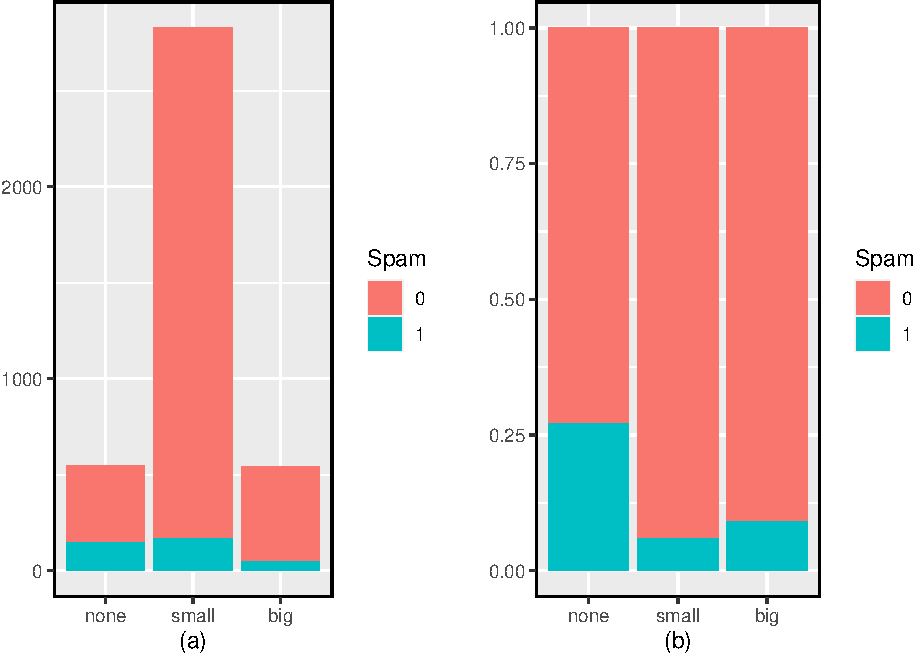
\includegraphics{_main_files/figure-latex/emailSpamNumberSegBarPlot-1.pdf}
\caption{\label{fig:emailSpamNumberSegBarPlot}(a) Gráficos de barras segmentadas para números encontrados em emails, onde as contagens foram divididas pela variável spam e (b) Versão normalizada}
\end{figure}

\begin{example}
\protect\hypertarget{exm:unnamed-chunk-38}{}{\label{exm:unnamed-chunk-38} }Examine os dois gráficos de barras segmentados. Qual é mais útil?
\end{example}

Pela Figura \ref{fig:emailSpamNumberSegBarPlot}, o primeiro gráfico contém mais informações, mas o segundo apresenta a informação mais claramente. Este segundo gráfico deixa claro que e-mails sem número têm uma taxa relativamente alta de e-mail de spam -- cerca de 27\%! Por outro lado, menos de 10\% de e-mail com números pequenos ou grandes são spam.

Como a proporção de spam é alterada entre os grupos na no segundo gráfico, Podemos concluir que as variáveis são dependentes, o que é algo que também conseguimos discernir usando proporções de tabela. Porque tanto o grupo nenhum quanto o grupo grande têm relativamente poucas observações em comparação com o grupo pequeno, a associação é mais difícil de ver na Figura \ref{fig:emailSpamNumberSegBarPlot}.

Em alguns outros casos, um gráfico de barras segmentado que não seja padronizado será mais útil na comunicação de informações importantes. Antes de estabelecer um gráfico de barras segmentado específico, crie formulários padronizados e não padronizados e decida qual deles é mais eficaz na comunicação de características dos dados.

\begin{figure}
\centering
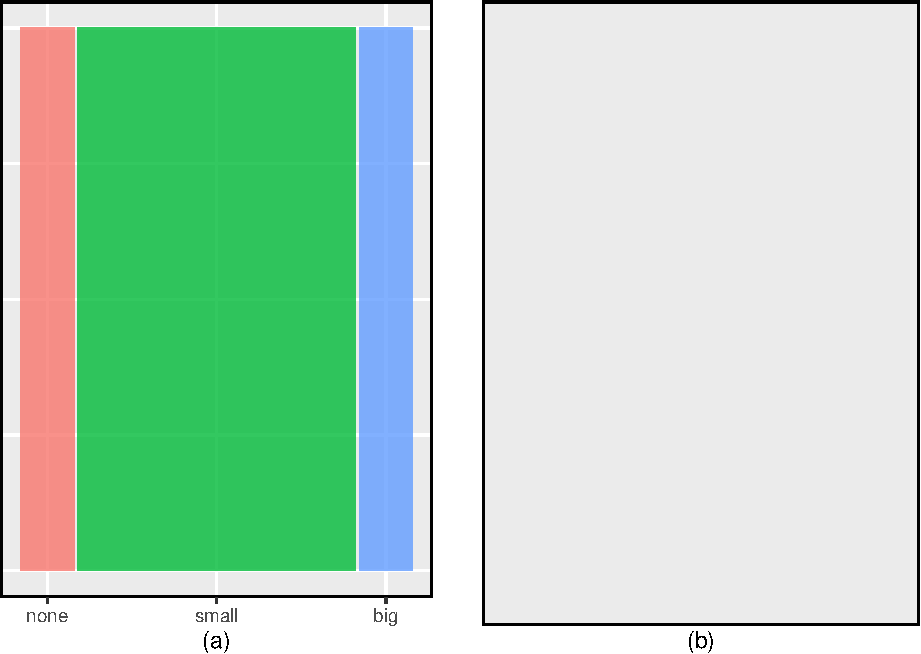
\includegraphics{_main_files/figure-latex/emailSpamNumberMosaicPlot-1.pdf}
\caption{\label{fig:emailSpamNumberMosaicPlot}(a) O mosaico de uma variável para número e (b) o mosaico de duas variáveis para ambos número e spam.}
\end{figure}

Um \textbf{gráfico de mosaico} é uma exibição gráfica de informações da tabela de contingência que é semelhante a um gráfico de barras para uma variável ou um gráfico de barras segmentadas ao usar duas variáveis. O primeiro plot da Figura \ref{fig:emailSpamNumberMosaicPlot} mostra um gráfico de mosaico para a variável \texttt{número}. Cada coluna representa um nível de \texttt{número}, e as larguras das colunas correspondem à proporção de e-mails para cada tipo de número. Por exemplo, há menos e-mails sem números do que e-mails com apenas números pequenos, portanto a coluna de e-mails não numerados é menor. Em geral, os gráficos de mosaico usam áreas para representar o número de observações que a caixa representa.

Esta plotagem em mosaico de uma variável é dividida em partes na segunda figura usando a variável \texttt{spam}. Cada coluna é dividida proporcionalmente de acordo com a fração de e-mails que eram spam em cada categoria de número. Por exemplo, a segunda coluna, representando e-mails com apenas números pequenos, foi dividida em e-mails que eram spam e não spam.

Como outro exemplo, a terceira coluna representa e-mails de spam que tinham números grandes, e a parte superior da terceira coluna representa e-mails regulares que tinham números grandes. Podemos novamente usar este gráfico para ver que as variáveis \texttt{spam} e \texttt{número} estão associadas, pois algumas colunas são divididas em diferentes localizações verticais do que outras, que é a mesma técnica usada para verificar uma associação na versão padronizada do gráfico de barras segmentadas.

\begin{figure}
\centering

\includegraphics{_main_files/figure-latex/emailSpamNumberMosaicRev-1.pdf}
\caption{\label{fig:emailSpamNumberMosaicRev}Gráfico em que os e-mails são agrupados pela variável número depois de terem sido divididos em spam e não spam.}
\end{figure}

De forma semelhante, um mosaico representando proporções da Tabela \ref{tab:emailSpamNumberTableTotals} poderia ser construído, como mostrado na Figura \ref{fig:emailSpamNumberMosaicRev}. No entanto, como é mais perspicaz para esse aplicativo considerar a fração de spam em cada categoria da variável \texttt{número}, preferimos a Figura \ref{fig:emailSpamNumberMosaicPlot}.

\hypertarget{onlyPizzaGraph}{%
\subsection{O único gráfico de pizza que você verá nesta apostila}\label{onlyPizzaGraph}}

Embora os gráficos de pizza sejam bem conhecidos, eles normalmente não são tão úteis quanto outros gráficos em uma análise de dados. Um \textbf{gráfico de pizza} é mostrado na Figura \ref{fig:emailNumberPieChart} ao lado de um gráfico de barra. Geralmente, é mais difícil comparar tamanhos de grupos em um gráfico de pizza do que em um gráfico de barras, especialmente quando as categorias têm contagens ou proporções quase idênticas. No caso das categorias nenhum e grande, a diferença é tão pequena que você pode ser incapaz de distinguir qualquer diferença nos tamanhos dos grupos para ambos os gráficos!

\begin{figure}
\centering
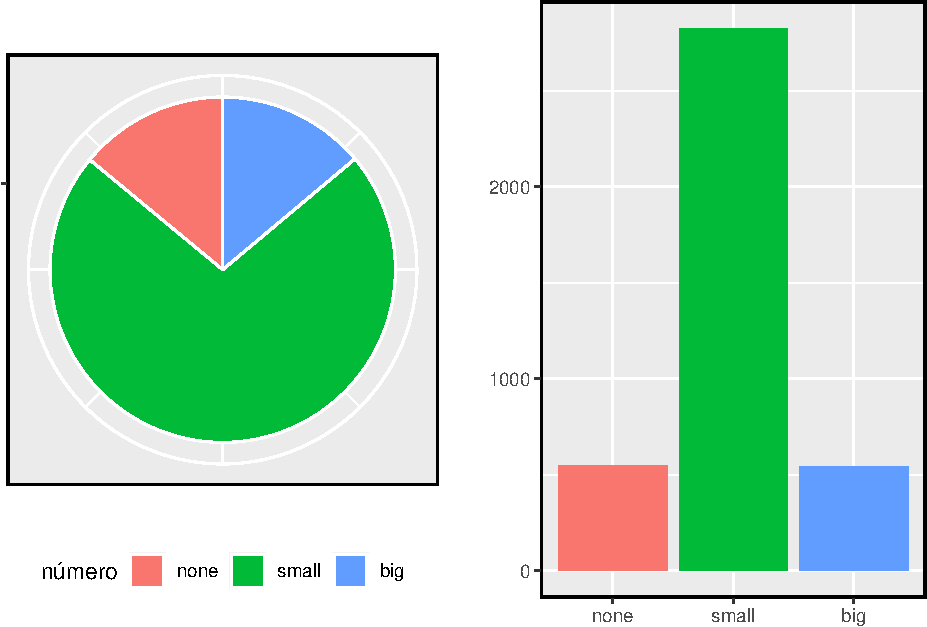
\includegraphics{_main_files/figure-latex/emailNumberPieChart-1.pdf}
\caption{\label{fig:emailNumberPieChart}Um gráfico de pizza e um gráfico de barras de número para o conjunto de dados email.}
\end{figure}

\hypertarget{comparingAcrossGroups}{%
\subsection{Comparando dados numéricos entre grupos}\label{comparingAcrossGroups}}

Algumas das investigações mais interessantes podem ser consideradas examinando dados numéricos entre grupos. Os métodos necessários aqui não são realmente novos. Tudo o que é necessário é fazer um gráfico numérico para cada grupo. Aqui dois métodos convenientes são introduzidos: box-plot lado a lado e histogramas.

Vamos dar uma olhada novamente no conjunto de dados \texttt{condado} e comparar a renda familiar média para os municípios, em comparação com os municípios que não tiveram ganho. Embora possamos gostar de estabelecer uma conexão causal aqui, lembre-se de que esses dados são observacionais e, portanto, tal interpretação seria injustificada.

Havia 2.041 municípios, onde a população aumentou de 2000 a 2010, e havia 1.099 municípios sem ganho (todos, exceto um, foram uma perda). Uma amostra aleatória de 100 municípios do primeiro grupo e 50 do segundo grupo são mostrados na Tabela \ref{tab:countyIncomeSplitByPopGainTable} para dar uma melhor noção de alguns dos dados brutos.

\begin{table}

\caption{\label{tab:countyIncomeSplitByPopGainTable}Nesta tabela, a renda familiar média (em 1000 dólares) de uma amostra aleatória de 100 municípios que ganharam população entre 2000-2010. Rendimentos médios de uma amostra aleatória de 50 municípios que não tiveram ganho de população são mostrados também}
\centering
\begin{tabular}[t]{l|l}
\hline
ganho populacional & nenhum ganho\\
\hline
41.2, 22.9, 47.9, 50.1, 57.4, 43.8, 41.3, 68.3, 42.6, 66.4 & 40.3, 29.5, 28, 38.1, 43.3\\
\hline
51.9, 44.5, 39.4, 43.8, 71.3, 50.2, 35.8, 33.1, 39.9, 36.4 & 43.7, 35.8, 46, 38.6, 37.6\\
\hline
27.3, 42.6, 26, 40.5, 48.3, 53.6, 41.4, 83.3, 34, 38.6 & 57.5, 46.2, 38.4, 36.4, 39.7\\
\hline
71.7, 36.3, 45.8, 40.4, 30.4, 31.4, 42.2, 37.5, 40.6, 33.8 & 21.4, 43.6, 33.5, 31.8, 39.1\\
\hline
68.3, 38.7, 50.7, 34.3, 46.3, 48.7, 40, 45.1, 36.4, 45.7 & 39.5, 37.5, 36.7, 38.7, 42.3\\
\hline
51.5, 37.3, 45.1, 43.2, 53.5, 48.8, 35.7, 31, 62, 35.1 & 31.9, 29.3, 32.6, 26.5, 46.7\\
\hline
38.9, 48.4, 45.2, 57.3, 32.2, 41,60.2, 66.4, 79.1, 50.6 & 41.5, 37, 29.3, 39.8, 34.8\\
\hline
31.8, 26.1, 28.1, 38.5, 46.7, 37.6, 30.6, 37.3, 40.8, 34.7 & 41.3, 42.8, 22.3, 47.1, 36\\
\hline
45.2, 63.3, 37, 53.1, 36.1, 34.5, 59.4, 36.9, 57.2, 29.4 & 39.8, 48.2, 31.1, 30.1, 31.1\\
\hline
42.3, 30.5, 32.2, 56.8, 41.7, 42.6, 32.2, 33.1, 54.7, 66.7 & 40.1, 25.9, 45.7, 37.7, 50.1\\
\hline
\end{tabular}
\end{table}

O \textbf{box-plot lado a lado} é uma ferramenta tradicional para comparação entre grupos. Um exemplo é mostrado no gráfico esquerdo da Figura \ref{fig:countyIncomeSplitByPopGain}, onde há dois gráficos, um para cada grupo, colocados em uma janela de plotagem e desenhados na mesma escala.

\begin{figure}
\centering
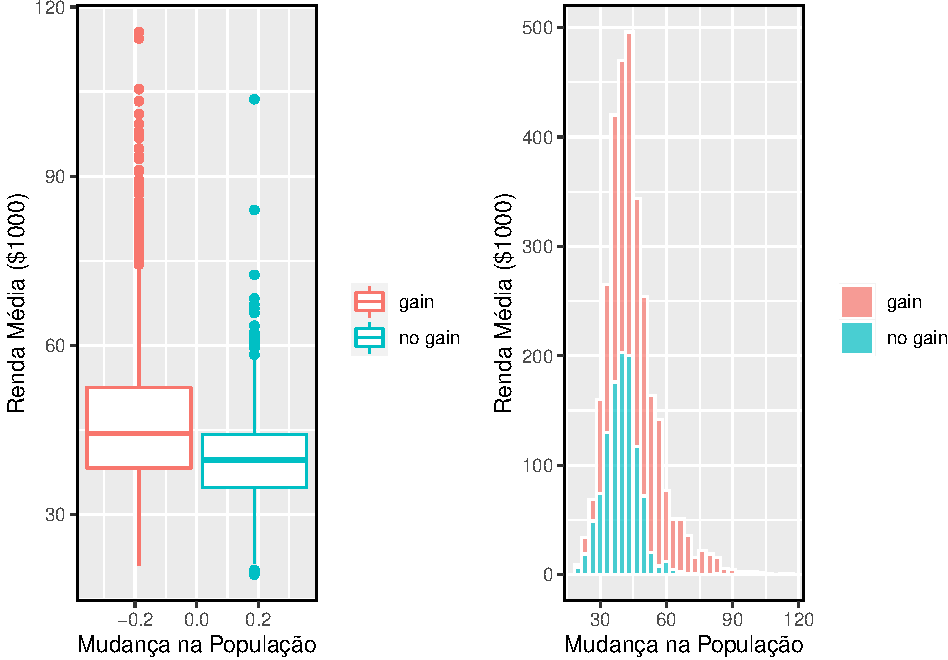
\includegraphics{_main_files/figure-latex/countyIncomeSplitByPopGain-1.pdf}
\caption{\label{fig:countyIncomeSplitByPopGain}Box-plot lado a lado e histogramas para a variável renda\_med, onde os municípios são divididos por se houce um ganho ou perda populacional de 2000 a 2010. Os dados de renda foram coletados entre 2006 e 2010.}
\end{figure}

Outro método de plotagem útil são \textbf{histogramas juntos} para comparar dados numéricos entre grupos. Estes são os histogramas de cada grupo colocados no mesmo enredo, como mostrado no gráfico do lado direito da Figura \ref{fig:countyIncomeSplitByPopGain}.

\begin{center}\rule{0.5\linewidth}{0.5pt}\end{center}

\begin{exercise}
\protect\hypertarget{exr:comparingPriceByTypeExercise}{}{\label{exr:comparingPriceByTypeExercise} }Use os gráficos na Figura \ref{fig:countyIncomeSplitByPopGain} para comparar os rendimentos para os municípios nos dois grupos. O que você percebe sobre o centro aproximado de cada grupo? O que você percebe sobre a variabilidade entre os grupos? A forma é relativamente consistente entre os grupos? Quantas modas \emph{proeminentes} existem para cada grupo?\footnote{As respostas podem variar um pouco. Os municípios com ganhos de população tendem a ter renda mais alta (mediana de cerca de \$45.000) versus municípios sem um ganho (mediana de cerca de \$40.000). A variabilidade também é um pouco maior para o grupo de ganho de população. Isso é evidente no IQR, que é cerca de 50\% maior no grupo ganho. Ambas as distribuições mostram inclinação a direita e são unimodais. Há um pequeno aumento secundário em torno de \$60.000 para o grupo sem ganho, visível no histograma, que parece fora de lugar. (Examinando o conjunto de dados, verificamos que 8 desses 15 municípios estão no Alasca e no Texas.) Os box-plots indicam que há muitas observações muito acima da mediana em cada grupo, embora devamos antecipar que muitas observações vão além ao se usar um conjunto de dados tão grande.}
\end{exercise}

\begin{center}\rule{0.5\linewidth}{0.5pt}\end{center}

\begin{center}\rule{0.5\linewidth}{0.5pt}\end{center}

\begin{exercise}
\protect\hypertarget{exr:unnamed-chunk-39}{}{\label{exr:unnamed-chunk-39} }Quais componentes de cada gráfico na Figura \ref{fig:countyIncomeSplitByPopGain} você acha mais útil?\footnote{As respostas irão variar. Os gráficos de box-plot lado-a-lado são especialmente úteis para comparar centros e variabilidades, enquanto os histogramas são mais úteis para ver a forma de distribuição, inclinação e grupos de anomalias.}
\end{exercise}

\begin{center}\rule{0.5\linewidth}{0.5pt}\end{center}

\hypertarget{caseStudyGenderDiscrimination}{%
\section{Estudo de caso: discriminação de gênero (tópico especial)}\label{caseStudyGenderDiscrimination}}

\begin{example}
\protect\hypertarget{exm:classRightLeftSideApple}{}{\label{exm:classRightLeftSideApple} }Suponha que seu professor divida os alunos da classe em dois grupos: alunos à esquerda e alunos à direita. Se \(\hat{p}_{_E}\) e \(\hat{p}_{_S}\) representam a proporção de alunos que possuem um produto da Apple à esquerda e à direita, respectivamente, você ficaria surpreso se \(\hat{p}_{_E}\) e \(\hat{p}_{_D}\)?\} não fossem exatamente iguais?
\end{example}

Embora as proporções provavelmente estivessem próximas umas das outras, seria incomum que elas fossem exatamente as mesmas. Nós provavelmente observaríamos uma pequena diferença devido ao \textbf{acaso}.

\begin{center}\rule{0.5\linewidth}{0.5pt}\end{center}

\begin{exercise}
\protect\hypertarget{exr:unnamed-chunk-40}{}{\label{exr:unnamed-chunk-40} }Se não achamos que o lado da sala em que uma pessoa está sentada na aula está relacionado a se ela possui um produto da Apple, que suposição estamos fazendo sobre a relação entre essas duas variáveis?\footnote{Nós estaríamos assumindo que essas duas variáveis são independentes.}
\end{exercise}

\begin{center}\rule{0.5\linewidth}{0.5pt}\end{center}

\hypertarget{variabilityWithinData}{%
\subsection{Variabilidade nos dados}\label{variabilityWithinData}}

Consideramos um estudo investigando a discriminação de gênero na década de 1970, que é definida no contexto das decisões de pessoal dentro de um banco\footnote{Rosen B e Jerdee T. 1974. Influência dos estereótipos do papel sexual nas decisões de pessoal. Journal of Applied Psychology 59 (1): 9-14.}. A pergunta de pesquisa que esperamos responder é

\begin{quote}
``As mulheres são discriminadas injustamente em decisões de promoção feitas por gerentes do sexo masculino?''
\end{quote}

Os participantes deste estudo são 48 supervisores bancários do sexo masculino que frequentam um instituto de gestão da Universidade da Carolina do Norte em 1972. Eles foram solicitados a assumir o papel de diretor de pessoal de um banco e receberam um arquivo pessoal para julgar se a pessoa deveria ser promovido a um cargo de gerente de filial. Os arquivos dados aos participantes eram idênticos, exceto que metade deles indicava que o candidato era do sexo masculino e a outra metade indicava que o candidato era do sexo feminino. Esses arquivos foram aleatoriamente atribuídos.

\begin{center}\rule{0.5\linewidth}{0.5pt}\end{center}

\begin{exercise}
\protect\hypertarget{exr:unnamed-chunk-41}{}{\label{exr:unnamed-chunk-41} }Isso é um estudo observacional ou um experimento? Que implicações o tipo de estudo tem sobre o que pode ser inferido dos resultados?\footnote{O estudo é uma experiência, pois os sujeitos foram aleatoriamente designados com um arquivo masculino ou um arquivo feminino. Como esse é um experimento, os resultados podem ser usados para avaliar uma relação causal entre gênero de um candidato e a decisão de promoção.}
\end{exercise}

\begin{center}\rule{0.5\linewidth}{0.5pt}\end{center}

Para cada supervisor, registramos o gênero associado ao arquivo atribuído e à decisão da promoção. Usando os resultados do estudo resumidos na Tabela \ref{tab:discriminationResults}, gostaríamos de avaliar se as mulheres são injustamente discriminadas nas decisões de promoção. Neste estudo, uma proporção menor de mulheres é promovida do que os homens (0.583 versus 0.875), mas não está claro se a diferença fornece \textbf{evidências convincentes} de que as mulheres são discriminadas injustamente.

\begin{table}

\caption{\label{tab:discriminationResults}Resultados resumidos para o estudo de discriminação de gênero.}
\centering
\begin{tabular}[t]{l|c|c|c}
\hline
  & Promovido & Não Promovido & Total\\
\hline
Homem & 21 & 3 & 24\\
\hline
Mulher & 14 & 10 & 24\\
\hline
Total & 35 & 13 & 48\\
\hline
\end{tabular}
\end{table}

\begin{example}
\protect\hypertarget{exm:discriminationResultsWhatIsConvincingEvidence}{}{\label{exm:discriminationResultsWhatIsConvincingEvidence} }Os estatísticos são às vezes chamados a avaliar a força da evidência. Ao olhar para as taxas de promoção para homens e mulheres neste estudo, o que vem à mente quando tentamos determinar se os dados mostram evidências convincentes de uma diferença real?
\end{example}

As taxas de promoção observadas (58,3\% para mulheres versus 87,5\% para homens) sugerem que pode haver discriminação contra as mulheres nas decisões de promoção. No entanto, não podemos ter certeza se a diferença observada representa discriminação ou se é apenas por acaso. Geralmente, há um pouco de flutuação nos dados da amostra, e não esperamos que as proporções da amostra sejam \emph{exatamente} iguais, mesmo que a verdade seja que as decisões de promoção eram independentes do gênero.

O Exemplo \ref{exm:discriminationResultsWhatIsConvincingEvidence} é um lembrete de que os resultados observados na amostra podem não refletir perfeitamente as relações verdadeiras entre as variáveis na população subjacente. A Tabela \ref{tab:discriminationResults} mostra que houve 7 menos promoções no grupo feminino do que no masculino, uma diferença nas taxas de promoção de 29.2\% \(\left( \frac{21}{24} - \frac{14}{24} = 0.292 \right)\). Essa diferença é grande, mas o tamanho da amostra para o estudo é pequeno, não ficando claro se essa diferença observada representa discriminação ou se é simplesmente por acaso. Nós rotulamos essas duas afirmações concorrentes, \(H_0\) e \(H_1\):

\begin{itemize}
\item
  \(H_0\): \textbf{Hipótese nula:} As variáveis gênero e decisão são independentes. Eles não têm nenhum relacionamento, e a diferença observada entre a proporção de homens e mulheres que foram promovidos, 29,2\%, deu-se pelo acaso.
\item
  \(H_A\): \textbf{Hipótese alternativa:} As variáveis gênero e decisão não são independentes. A diferença nas taxas de promoção de 29,2\% não se deve ao acaso, e as mulheres igualmente qualificadas são menos propensas a serem promovidas do que os homens.
\end{itemize}

O que significaria se o modelo de independência, que diz que as variáveis gênero e decisão não estão relacionadas, é verdade? Isso significaria que cada banqueiro iria decidir se promoveria o candidato sem considerar o gênero indicado no arquivo. A diferença nas porcentagens de promoção se deu à maneira como os arquivos foram aleatoriamente divididos entre os banqueiros, e a aleatorização acabou dando origem a uma diferença relativamente grande de 29,2\%.

Considere o modelo alternativo: os banqueiros foram influenciados por qual gênero foi listado no arquivo pessoal. Se isso fosse verdade, e especialmente se essa influência fosse substancial, esperaríamos ver alguma diferença nas taxas de promoção de candidatos do sexo masculino e feminino. Se esse viés de gênero fosse contra as mulheres, esperaríamos uma fração menor das decisões de promoção para os arquivos de pessoal feminino em relação aos arquivos masculinos.

Escolhemos entre essas duas afirmações concorrentes, avaliando se os dados conflitam tanto com \(H_0\) que o modelo de independência não pode ser considerado razoável. Se este for o caso, e os dados suportarem \(H_1\), então rejeitaremos a noção de independência e concluiremos que houve discriminação.

\hypertarget{simulatingTheStudy}{%
\subsection{Simulando o estudo}\label{simulatingTheStudy}}

A Tabela \ref{tab:discriminationResults} mostra que 35 supervisores bancários recomendaram promoção e 13 não o fizeram. Agora, suponha que as decisões dos banqueiros fossem independentes do gênero. Então, se conduzirmos o experimento novamente com um arranjo aleatório diferente de arquivos, as diferenças nas taxas de promoção seriam baseadas apenas na flutuação aleatória. Na verdade, podemos realizar essa \emph{randomização}, que simula o que teria acontecido se as decisões dos banqueiros tivessem sido independentes do gênero, mas tivéssemos distribuído os arquivos de maneira diferente.

Nesta simulação, nós misturamos 48 arquivos pessoais, 24 rotulados \emph{masculino} e 24 rotulados \emph{femininos} e processe esses arquivos em duas pilhas. Vamos distribuir 35 arquivos na primeira pilha, o que representará os 35 supervisores que recomendaram a promoção. A segunda pilha terá 13 arquivos e representará os 13 supervisores que recomendaram contra a promoção. Então, como fizemos com os dados originais, tabulamos os resultados e determinamos a fração de homens e mulheres que foram promovidos. A randomização de arquivos nesta simulação é independente das decisões de promoção, o que significa que qualquer diferença nas duas frações é inteiramente devido ao acaso. A Tabela \ref{tab:discriminationRand1} mostra os resultados de tal simulação.

\begin{table}

\caption{\label{tab:discriminationRand1}Resultados da simulação, em que qualquer diferença nas taxas de promoção entre homens e mulheres é puramente devido ao acaso.}
\centering
\begin{tabular}[t]{l|c|c|c}
\hline
  & Promovido & Não Promovido & Total\\
\hline
Homem & 18 & 6 & 24\\
\hline
Mulher & 17 & 7 & 24\\
\hline
Total & 35 & 13 & 48\\
\hline
\end{tabular}
\end{table}

\begin{center}\rule{0.5\linewidth}{0.5pt}\end{center}

\begin{exercise}
\protect\hypertarget{exr:sampleDifferenceInMaleAndFemaleDiscrimination}{}{\label{exr:sampleDifferenceInMaleAndFemaleDiscrimination} }Qual é a diferença nas taxas de promoção entre os dois grupos simulados na Tabela \ref{tab:discriminationRand1}? Como isso se compara aos 29,2\% observados nos grupos reais?\footnote{\(18/24 - 17/24 = 0,042\) ou cerca de 4,2\% em favor dos homens. Essa diferença devido ao acaso é muito menor que a diferença observada nos grupos reais.}
\end{exercise}

\begin{center}\rule{0.5\linewidth}{0.5pt}\end{center}

\hypertarget{checkingIndependence}{%
\subsection{Checando independência}\label{checkingIndependence}}

Calculamos uma diferença possível sob o modelo de independência na Prática Orientada \ref{exr:sampleDifferenceInMaleAndFemaleDiscrimination}, que representa uma diferença devido ao acaso. Enquanto nesta primeira simulação, nós distribuímos arquivos fisicamente, é mais eficiente executar esta simulação usando um computador. Repetindo a simulação em um computador, temos outra diferença devido ao acaso: -0,042. E outro: 0,208. E assim por diante, até repetirmos a simulação suficientemente para termos uma boa idéia do que representa a \textbf{distribuição das diferenças do acaso}. A Figura \ref{fig:discRandDotPlot} mostra um gráfico das diferenças encontradas em 100 simulações, onde cada ponto representa uma diferença simulada entre as proporções de arquivos masculinos e femininos que foram recomendadas para promoção.

\begin{figure}
\centering
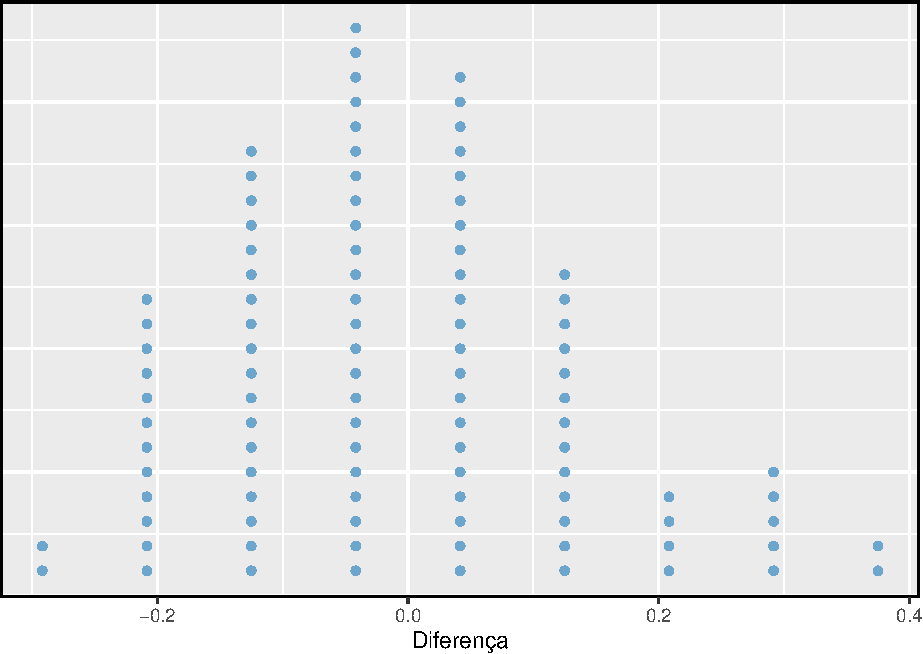
\includegraphics{_main_files/figure-latex/discRandDotPlot-1.pdf}
\caption{\label{fig:discRandDotPlot}Um gráfico de pontos empilhados de diferenças de 100 simulações produzidas sob o modelo independente, H0, onde gênero e decisão são independentes. Duas das 100 simulações apresentaram diferença de pelo menos 29.2\%, diferença observada no estudo.}
\end{figure}

Observe que a distribuição dessas diferenças simuladas é centralizada em torno de 0. Simulamos essas diferenças assumindo que o modelo de independência era verdadeiro e, sob essa condição, esperamos que a diferença seja zero com alguma flutuação aleatória. Nós geralmente ficariamos surpresos ao ver uma diferença de exatamente 0: às vezes, apenas por acaso, a diferença é maior que 0, e outras vezes é menor que zero.

\begin{example}
\protect\hypertarget{exm:unnamed-chunk-42}{}{\label{exm:unnamed-chunk-42} }Quantas vezes você observaria uma diferença de pelo menos 29,2\% (0,292) de acordo com a Figura \ref{fig:discRandDotPlot}? Muitas vezes, às vezes, raramente ou nunca?
\end{example}

Parece que uma diferença de pelo menos 29,2\% devido ao acaso só aconteceria em torno de 2\% do tempo, de acordo com a Figura \ref{fig:discRandDotPlot}. Uma probabilidade tão baixa indica um evento raro.

A diferença de 29,2\% sendo um evento raro sugere duas possíveis interpretações dos resultados do estudo:

\begin{itemize}
\item
  \(H_0\) \textbf{Modelo independente.} O gênero não tem efeito sobre a decisão de promoção, e observamos uma diferença que só aconteceria raramente.
\item
  \(H_1\) \textbf{Modelo alternativo.} O gênero tem um efeito sobre a decisão de promoção, e o que observamos foi, na verdade, devido a mulheres igualmente qualificadas serem discriminadas nas decisões de promoção, o que explica a grande diferença de 29,2\%.
\end{itemize}

Com base nas simulações, temos duas opções:

\begin{itemize}
\item
  \begin{enumerate}
  \def\labelenumi{(\arabic{enumi})}
  \tightlist
  \item
    Concluímos que os resultados do estudo não fornecem fortes evidências contra o modelo de independência. Ou seja, não temos evidências suficientemente fortes para concluir que houve discriminação de gênero.
  \end{enumerate}
\item
  \begin{enumerate}
  \def\labelenumi{(\arabic{enumi})}
  \setcounter{enumi}{1}
  \tightlist
  \item
    Concluímos que a evidência é suficientemente forte para rejeitar \(H_0\) e afirmar que houve discriminação de gênero. Quando conduzimos estudos formais, geralmente rejeitamos a noção de que acabamos de observar um evento raro.\footnote{Este raciocínio geralmente não se estende a observações anedóticas. Cada um de nós observa eventos incrivelmente raros todos os dias, eventos que não poderíamos esperar prever. No entanto, no cenário não rigoroso de evidência anedótica, quase tudo pode parecer um evento raro, então a ideia de procurar eventos raros nas atividades do dia a dia é traiçoeira. Por exemplo, podemos olhar para a loteria: havia apenas 1 em 176 milhões de chances que os números para o maior jackpot da história (30 de março de 2012) seriam (2, 4, 23, 38, 46) com uma Mega de 23, mas mesmo assim esses números surgiram! No entanto, independentemente dos números, eles teriam as mesmas probabilidades incrivelmente raras. Ou seja, \textbf{qualquer conjunto de números que poderíamos ter observado seria extremamente raro}. Esse tipo de situação é típico de nossas vidas diárias: cada evento possível em si parece incrivelmente raro, mas, se considerarmos todas as alternativas, esses resultados também são incrivelmente raros. Devemos ser cautelosos para não interpretar erroneamente tal evidência anedótica.} Assim, neste caso, rejeitamos o modelo de independência em favor da alternativa. Ou seja, estamos concluindo que os dados fornecem fortes evidências de discriminação de gênero contra as mulheres pelos supervisores.
  \end{enumerate}
\end{itemize}

Um campo de estatística, inferência estatística, é construído sobre a avaliação se tais diferenças são devidas ao acaso. Na inferência estatística, os estatísticos avaliam qual modelo é mais razoável, dados os dados. Ocorrem erros, assim como eventos raros, e podemos escolher o modelo errado. Embora nem sempre escolhamos corretamente, a inferência estatística nos fornece ferramentas para controlar e avaliar com que frequência esses erros ocorrem. Mais a frente, damos uma introdução formal ao problema da seleção de modelos. A seguir construiremos uma base de probabilidade e teoria necessária para tornar essa discussão rigorosa.

\begin{center}\rule{0.5\linewidth}{0.5pt}\end{center}

This work is licensed under a Creative Commons Attribution-ShareAlike 3.0 Unported License.

\hypertarget{ch2-prob}{%
\chapter{Probabilidade (tópico especial)}\label{ch2-prob}}

Probabilidade forma uma base para a estatística, e você pode já estar familiarizado com muitos aspectos da probabilidade. No entanto, a formalização dos conceitos é nova para a maioria. Este capítulo tem como objetivo introduzir a probabilidade em termos familiares usando processos que a maioria das pessoas já viu antes.

\hypertarget{basicsOfProbability}{%
\section{Definindo probabilidade (tópico especial)}\label{basicsOfProbability}}

\begin{example}
\protect\hypertarget{exm:probOf1}{}{\label{exm:probOf1} }Um dado é um cubo com seis faces numeradas 1, 2, 3, 4, 5 e 6. Qual é a chande de conseguir 1 ao jogar o dado?
\end{example}

Se o dado é honesto, então a chance de um 1 é tão provável quanto a chance de qualquer outro número. Como há seis resultados, a chance deve ser de 1 em 6 ou, equivalentemente, \(1/6\).

\begin{example}
\protect\hypertarget{exm:probOf1Or2}{}{\label{exm:probOf1Or2} }Qual é a chance de conseguir um 1 ou 2 na próxima rodada?
\end{example}

1 e 2 constituem dois dos seis resultados igualmente prováveis, então a chance de obter um desses dois resultados deve ser \(2/6 = 1/3\).

\begin{example}
\protect\hypertarget{exm:probOf123456}{}{\label{exm:probOf123456} }Qual é a chance de conseguir 1, 2, 3, 4, 5 ou 6 na próima rodada?
\end{example}

100\%. O resultado deve ser um desses números.

\begin{example}
\protect\hypertarget{exm:probNot2}{}{\label{exm:probNot2} }Qual é a chande de não sair um 2?
\end{example}

Já que a chance de cair um 2 é \(1/6\) ou \(16.66\%\), a chance de não cair um 2 deve ser \(100\% - 16.66\% = 83.33\%\) ou \(5/6\).

Alternativamente, poderíamos ter notado que não caindo 2 é o mesmo que conseguir um 1, 3, 4, 5, ou 6, que compõe cinco dos seis resultados igualmente prováveis e tem probabilidade \(5/6\).

\begin{example}
\protect\hypertarget{exm:probOf2Ones}{}{\label{exm:probOf2Ones} }Considere jogar dois dados. Se \(1/6\) das vezes em que o primeiro dado é um 1 e \(1/6\) das vezes o segundo dado é um 1, qual é a chance de conseguir dois 1s?
\end{example}

Se em \(1/6\) das vezes o primeiro dado é um 1 e \(1/6\) dessas vezes o segundo dado também é um 1, então a chance de que ambos os dados são 1 é \((1/6)\times (1/6)\) ou \(1/36\).

\hypertarget{probability}{%
\subsection{Probabilidade}\label{probability}}

Usamos probabilidade para construir ferramentas para descrever e entender a aparente aleatoriedade. Nós geralmente enquadramos a probabilidade em termos de um \textbf{processo aleatório} dando origem a um \texttt{resultado}.

\(\text{Jogue um dado} \longrightarrow 1, 2, 3, 4, 5 \text{ ou } 6\)

\(\text{Jogue uma moeda} \longrightarrow \text{cara, coroa}\)

Jogar um dado ou jogar uma moeda é um processo aparentemente aleatório e cada um dá origem a um resultado.

Probabilidade: A probabilidade de um resultado é a proporção de vezes que o resultado ocorreria se observássemos o processo aleatório um número infinito de vezes.

A probabilidade é definida como uma proporção e sempre recebe valores no intervalo fechado de 0 a 1. Também pode ser exibido como uma porcentagem entre 0\% e 100\%.

A probabilidade pode ser ilustrada jogando um dado muitas vezes. \(\hat{p}_n\) é a proporção de resultados que são 1 após as primeiras \(n\) jogadas. À medida que o número de jogadas aumenta, \(\hat{p}_n\) irá convergir para a probabilidade de jogar um 1, \(p = 1/6\). A Figura \ref{fig:dieProp} mostra essa convergência para 100.000 jogadas de dados. A tendência de \(\hat{p}_n\) estabilizar em torno de \(p\) é descrito pela \textbf{Lei dos Grandes Números}.

\begin{figure}
\centering
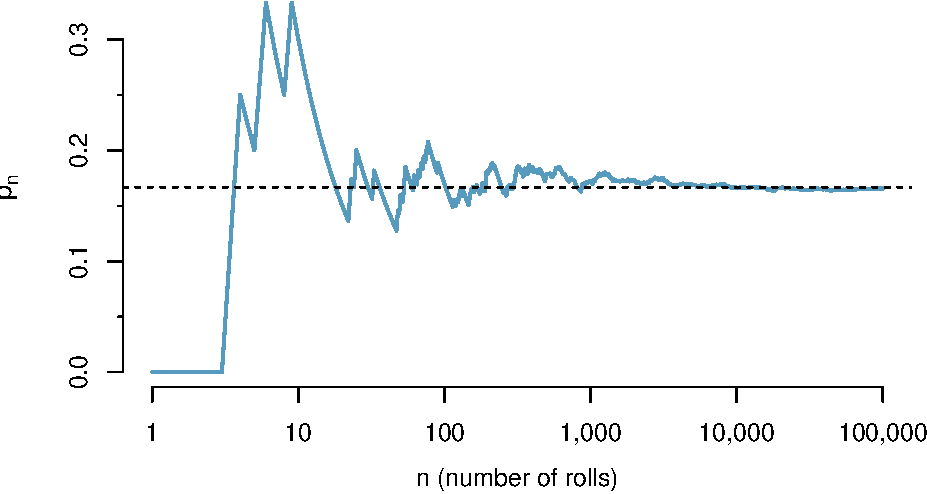
\includegraphics{_main_files/figure-latex/dieProp-1.pdf}
\caption{\label{fig:dieProp}A fração de jogadas de dados que deram 1 em cada estágio de uma simulação. A proporção tende a se aproximar da probabilidade 1/6 à medida que o número de jogadas aumenta.}
\end{figure}

Lei dos Grandes Números À medida que mais observações são coletadas, a proporção \(\hat{p}_n\) de ocorrências com um determinado resultado converge para a probabilidade \(p\) desse resultado.

Ocasionalmente, a proporção se desviará da probabilidade e parecerá desafiar a Lei dos Grandes Números, como acontece com \(\hat{p}_n\) muitas vezes, pela Figura \ref{fig:dieProp}. No entanto, esses desvios diminuem à medida que o número de jogadas aumenta.

Acima, escrevemos \(p\) como a probabilidade de lançar um 1. Também podemos escrever essa probabilidade como

\begin{eqnarray*}
P(\text{lançar um 1})
\end{eqnarray*}

À medida que nos tornarmos mais confortáveis com essa notação, vamos abreviá-la ainda mais. Por exemplo, se está claro que o processo é ``jogar um dado'', nós poderíamos abreviar \(P(\)lançando um 1\()\) como \(P(1)\).

\begin{center}\rule{0.5\linewidth}{0.5pt}\end{center}

\begin{exercise}
\protect\hypertarget{exr:randomProcessExercise}{}{\label{exr:randomProcessExercise} }
Processos aleatórios incluem jogar um dado e lançar uma moeda. (a) Pense em outro processo aleatório. (b) Descreva todos os resultados possíveis desse processo. Por exemplo, jogar um dado é um processo aleatório com possíveis resultados \(1, 2, \dots, 6\).\footnote{Aqui estão quatro exemplos. (i) Se alguém fica doente no próximo mês ou não é um processo aparentemente aleatório com os resultados \emph{doente} e \emph{não doente}. (ii) Podemos gerar um processo aleatório escolhendo aleatoriamente uma pessoa e medindo a altura dessa pessoa. O resultado deste processo será um número positivo. (iii) Se o mercado de ações sobe ou desce na próxima semana é um processo aparentemente aleatório com possíveis resultados \emph{cima}, \emph{baixo}, e \emph{sem mudança}. Alternativamente, poderíamos ter usado a variação percentual no mercado de ações como um resultado numérico. (iv) Se o seu colega de quarto limpa os seus pratos esta noite, provavelmente parece ser um processo aleatório com possíveis resultados \emph{limpa} e \emph{não limpa}.}
\end{exercise}

\begin{center}\rule{0.5\linewidth}{0.5pt}\end{center}

O que pensamos como processos aleatórios não são necessariamente aleatórios, mas podem ser muito difíceis de entender exatamente. O quarto exemplo na solução de nota de rodapé para a Prática Orientada \ref{exr:randomProcessExercise} sugere que o comportamento de um colega de quarto é um processo aleatório. No entanto, mesmo que o comportamento de um colega de quarto não seja verdadeiramente aleatório, modelar seu comportamento como um processo aleatório ainda pode ser útil.

Modelando um processo como aleatório Pode ser útil modelar um processo como aleatório, mesmo que não seja verdadeiramente aleatório.

\hypertarget{disjointMutuallyExclusiveResults}{%
\subsection{Resultados disjuntos ou mutuamente exclusivos}\label{disjointMutuallyExclusiveResults}}

Dois resultados são chamados de \textbf{disjuntos} ou \textbf{mutuamente exclusivos} se ambos não puderem acontecer. Por exemplo, se jogarmos um dado, os resultados 1 e 2 são disjuntos, pois não podem ocorrer. Por outro lado, os resultados 1 e \emph{jogar um número ímpar} não são disjuntos, pois ambos ocorrem se o resultado do teste for um 1. Os termos \textbf{disjunto} e \textbf{mutuamente exclusivos} são equivalentes e intercambiáveis.

Calcular a probabilidade de desfechos desarticulados é fácil. Ao jogar um dado, os resultados 1 e 2 são disjuntos e calculamos a probabilidade de que um desses resultados ocorra, adicionando suas probabilidades separadas:

\begin{eqnarray*}
P(\text{1 ou 2}) = P(\text{1}) + P(\text{2}) = 1/6 + 1/6 = 1/3
\end{eqnarray*}

Quanto à probabilidade de lançar um 1, 2, 3, 4, 5, ou 6? Aqui, novamente, todos os resultados são disjuntos, então adicionamos as probabilidades:

\begin{eqnarray*}
&&P(\text{1 ou 2 ou 3 ou 4 ou 5 ou 6}) \\
    &&\quad= P(\text{1})+P(\text{2})+P(\text{3})+P(\text{4})+P(\text{5})+P(\text{6}) \\
    &&\quad= 1/6 + 1/6 + 1/6 + 1/6 + 1/6 + 1/6 = 1.
\end{eqnarray*}

A \textbf{Regra da Adição} garante a precisão desta abordagem quando os resultados são disjuntos.

Regra da adição de resultados disjuntos Se \(A_1\) e \(A_2\) representam dois desfechos disjuntos, então a probabilidade de que um deles ocorra é dada por

\begin{eqnarray*}
P(A_1\text{ ou } A_2) = P(A_1) + P(A_2)
\end{eqnarray*}

Se houver muitos resultados disjuntos \(A_1,\dots, A_k\), então a probabilidade de que um desses resultados ocorra é

\begin{eqnarray}
P(A_1) + P(A_2) + \cdots + P(A_k)
\end{eqnarray}

\begin{center}\rule{0.5\linewidth}{0.5pt}\end{center}

\begin{exercise}
\protect\hypertarget{exr:unnamed-chunk-43}{}{\label{exr:unnamed-chunk-43} }Estamos interessados na probabilidade de rolar um 1, 4, ou 5: (a) Explicar porque os resultados 1, 4, e 5 são disjuntos. (b) Aplicar a Regra da Adição para resultados disjuntos para determinar \(P(1 ou 4 ou 5)\).\footnote{(a) O processo aleatório é jogar um dado e, no máximo, um desses resultados pode surgir. Isso significa que eles são resultados disjuntos (b) \(P(1 ou 4 ou 5\)) = \(P(1) + P(4) + P(5) = \frac{1}{6} + \frac{1}{6} + \frac{1}{6} = \frac{3}{6} = \frac{1}{2}\)}
\end{exercise}

\begin{center}\rule{0.5\linewidth}{0.5pt}\end{center}

\begin{center}\rule{0.5\linewidth}{0.5pt}\end{center}

\begin{exercise}
\protect\hypertarget{exr:unnamed-chunk-44}{}{\label{exr:unnamed-chunk-44} }No banco de dados \texttt{email} da introdução, a variável \emph{número} descreveu se nenhum número, apenas um ou mais números pequenos, ou se pelo menos um grande número apareceu em um email. Dos 3.921 e-mails, 549 não tinham números, 2.827 tinham apenas um ou mais números pequenos e 545 tinham pelo menos um número grande: (a) Os resultados \textbf{nenhum}, \textbf{pequeno}, e \textbf{grande} são disjuntos? (b) Determinar a proporção de emails com valor \textbf{pequeno} e \textbf{grande}, separadamente. (c) Use a Regra da Adição para resultados disjuntos para calcular a probabilidade de um e-mail selecionado aleatoriamente do conjunto de dados ter um número, pequeno ou grande.\footnote{(a) Sim. Cada email é categorizado em apenas um nível de número. (b) Pequeno: \(\frac{2827}{3921} = 0.721\). Grande: \(\frac{545}{3921} = 0.139\). (c) \(P(\text{pequeno ou grande}) = P(\text{pequeno}) + P(\text{grande}) = 0.721 + 0.139 = 0.860\).}
\end{exercise}

\begin{center}\rule{0.5\linewidth}{0.5pt}\end{center}

Suponha que \(A\) representa o evento no qual um lançamento de dados resulta 1 ou 2 e \(B\) representa o evento que o dado é um 4 ou 6. Escrevemos \(A\) como o conjunto de resultados \(\{1,2\}\) e \(B = \{4, 6\}\). Esses conjuntos são comumente chamados de \textbf{eventos}. Como \(A\) e \(B\) não possuem elementos em comum, eles são eventos disjuntos. \(A\) e \(B\) estão representados na Figura \ref{fig:disjointSets}.

\begin{figure}
\centering
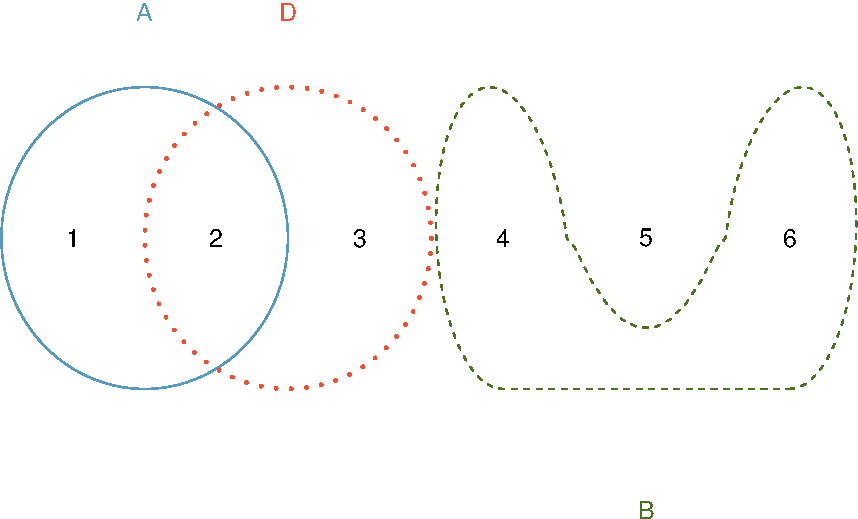
\includegraphics{_main_files/figure-latex/disjointSets-1.pdf}
\caption{\label{fig:disjointSets}Três eventos, A, B e D, consistem em resultados do lançamento de um dado. A e B são disjuntos, pois não tem nenhum resultado em comum.}
\end{figure}

A Regra da Adição aplica-se tanto a resultados disjuntos quanto a eventos disjuntos. A probabilidade de que um dos eventos disjuntos \(A\) ou \(B\) ocorra é a soma das probabilidades separadas:

\begin{align*}
P(A\text{ ou }B) = P(A) + P(B) = 1/3 + 1/3 = 2/3
\end{align*}

\begin{center}\rule{0.5\linewidth}{0.5pt}\end{center}

\begin{exercise}
\protect\hypertarget{exr:unnamed-chunk-45}{}{\label{exr:unnamed-chunk-45} }(a) Verifique a probabilidade do evento \(A\), \(P(A) = 1/3\) usando a Regra da Adição.
(b) Faça o mesmo para o evento \(B\).\footnote{(a) \(P(A) = P(1 ou 2) = P(1) + P(2) = \frac{1}{6} + \frac{1}{6} = \frac{2}{6} = \frac{1}{3}\). (b) Similarmente, \(P(B) = 1/3\).}
\end{exercise}

\begin{center}\rule{0.5\linewidth}{0.5pt}\end{center}

\begin{center}\rule{0.5\linewidth}{0.5pt}\end{center}

\begin{exercise}
\protect\hypertarget{exr:exerExaminingDisjointSetsABD}{}{\label{exr:exerExaminingDisjointSetsABD} }(a) Usando Figura \ref{fig:disjointSets} como referência, que resultados são representados pelo evento \(D\)?
(b) Os eventos \(B\) e \(D\) são disjuntos?
(c) Os eventos \(A\) e \(D\) são disjuntos?\footnote{(a) Resultados 2 e 3. (b) Sim, Os eventos \(B\) e \(D\) são disjuntos porque não compartilham resultados. (c) Os eventos \(A\) e \(D\) compartilham um resultado em comum, 2, e portanto não são disjuntos}
\end{exercise}

\begin{center}\rule{0.5\linewidth}{0.5pt}\end{center}

\begin{center}\rule{0.5\linewidth}{0.5pt}\end{center}

\begin{exercise}
\protect\hypertarget{exr:unnamed-chunk-46}{}{\label{exr:unnamed-chunk-46} }Na Prática Orientada \ref{exr:exerExaminingDisjointSetsABD}, você confirmou que \(B\) e \(D\) da Figura \ref{fig:disjointSets} são disjuntos. Calcule a probabilidade de que o evento \(B\) ou evento \(D\) ocorra.\footnote{Como \(B\) e \(D\) são eventos disjuntos, use a regra da adição: \(P(B \text{ ou } D) = P(B) + P(D) = \frac{1}{3} + \frac{1}{3} = \frac{2}{3}\).}
\end{exercise}

\begin{center}\rule{0.5\linewidth}{0.5pt}\end{center}

\hypertarget{probabilityEventsNotDisjoint}{%
\subsection{Probabilidades quando os eventos não são disjuntos}\label{probabilityEventsNotDisjoint}}

Vamos considerar cálculos para dois eventos que não são disjuntos no contexto de um \textbf{baralho padrão de 52 cartas}. Se você não estiver familiarizado com as cartas em um baralho regular, consulte a nota de rodapé.\^{}{[}As 52 cartas são divididas em quatro naipes: \(\clubsuit\) (paus), \(\diamondsuit\) (ouros), \(\heartsuit\) (copas) e \(\spadesuit\) (espadas). Cada naipe tem suas 13 cartas rotulados: \(2, 3, \dots, 10, J (valete), Q (rainha), K (rei), e A (ás)\). Assim, cada carta é uma combinação única de um naipe e um rótulo, por exemplo 4\(\heartsuit\) e J\(\clubsuit\). As 12 cartas representadas pelos valetes, rainhas e reis são chamadas figuras. As cartas que são \(\diamondsuit\) ou \(\heartsuit\) são tipicamente vermelhas enquanto os outros dois naipes são tipicamente de cor preta.

\begin{center}\rule{0.5\linewidth}{0.5pt}\end{center}

\begin{exercise}
\protect\hypertarget{exr:unnamed-chunk-47}{}{\label{exr:unnamed-chunk-47} }(a) Qual é a probabilidade de uma carta selecionada aleatoriamente ser um ouro?
(b)Qual é a probabilidade de uma carta selecionada aleatoriamente ser um carta de figura?\footnote{(a) Existem 52 cartas e 13 ouros. Se as cartas são embaralhadas, cada carta tem uma chance igual de ser sorteada, então a probabilidade de uma carta selecionada aleatoriamente ser um ouro é \(P(\diamondsuit) = \frac{13}{52} = 0.250\). (b) Da mesma forma, existem 12 figuras, então \(P(\text{figuras}) = \frac{12}{52} = \frac{3}{13} = 0.231\).}
\end{exercise}

\begin{center}\rule{0.5\linewidth}{0.5pt}\end{center}

Os \textbf{Diagramas de Venn} são úteis quando os resultados podem ser categorizados como dentro ou fora para duas ou três variáveis, atributos ou processos aleatórios. O diagrama de Venn na Figura \ref{fig:cardsDiamondFaceVenn} usa um círculo para representar ouros e outro para representar cartas de figura. Se uma carta é um ouro e uma carta de figura, ela cai na interseção dos círculos. Se for um ouro, mas não uma carta de figura, ele será parte do círculo esquerdo que não está no círculo direito (e assim por diante). O número total de cartas que são ouro é dado pelo número total de cartas no círculo de ouros: \(10+3=13\). As probabilidades também são mostradas (por ex. \(10/52 = 0.1923\)).

\begin{figure}
\centering
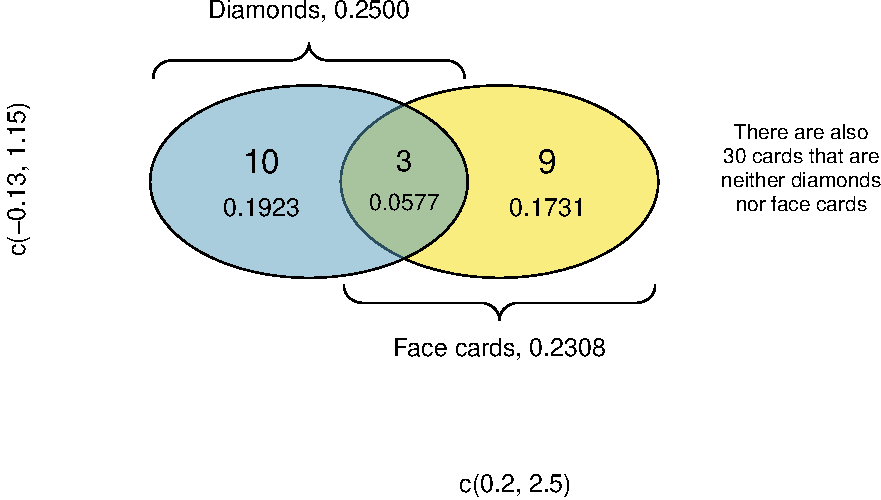
\includegraphics{_main_files/figure-latex/cardsDiamondFaceVenn-1.pdf}
\caption{\label{fig:cardsDiamondFaceVenn}Um diagrama de Venn para ouros e cartas de figura.}
\end{figure}

\begin{center}\rule{0.5\linewidth}{0.5pt}\end{center}

\begin{exercise}
\protect\hypertarget{exr:unnamed-chunk-48}{}{\label{exr:unnamed-chunk-48} }Utilizando a Figura \ref{fig:cardsDiamondFaceVenn}, verifique que \(P(\text{figura}) = 12/52 = 3/13\)\footnote{O diagrama de Venn mostra que as cartas figuras estão separadas em: \emph{carta de figura mas não é de ouro} e \emph{carta de figura e de ouro}. Já que são eventos disjuntos, a probabilidade é dada pela soma das probabilidades dos dois eventos \(\frac{3}{52} + \frac{9}{52} = \frac{12}{52} = \frac{3}{13}\)}
\end{exercise}

\begin{center}\rule{0.5\linewidth}{0.5pt}\end{center}

\(A\) representa o evento em que uma carta selecionada aleatoriamente é um ouro e \(B\) representa o evento que é uma carta de figura. Como calculamos \(P(A \text{ ou } B)\)? Eventos \(A\) e \(B\) não são disjuntos -- as cartas \(J\diamondsuit, Q\diamondsuit\), e \(K\diamondsuit\) caem em ambas as categorias - por isso não podemos usar a Regra da Adição para eventos disjuntos. Em vez disso, usamos o diagrama de Venn. Começamos adicionando as probabilidades dos dois eventos:

\begin{eqnarray}
P(A) + P(B)
  = P({\diamondsuit}) + P(\text{figuras})
  = 13/52 + 12/52
  \label{eq:overCountFaceDiamond}
\end{eqnarray}

No entanto, as três cartas que estão em ambos os eventos foram contadas duas vezes, uma vez em cada probabilidade. Devemos corrigir essa contagem dupla:

\begin{eqnarray}
P(A\text{ ou } B) &=&P(\diamondsuit\text{ ou figura}) \\
  &=& P({\diamondsuit}) + P(\text{figura}) - P({\diamondsuit}\text{ e figura})  \\
  &=& 13/52 + 12/52 - 3/52 \\
  &=& 22/52 = 11/26 
    \label{eq:diamondFace}
\end{eqnarray}

A Equação \eqref{eq:diamondFace} é um exemplo da \textbf{Regra Geral da Adição}.

Regra Geral da Adição Se \(A\) e \(B\) são quaisquer dois eventos, disjuntos ou não, então a probabilidade de que pelo menos um deles ocorra é

\begin{eqnarray}
P(A\text{ ou }B) = P(A) + P(B) - P(A\text{ e }B)
\label{eq:generalAdditionRule}
\end{eqnarray}

onde \(P(A \text{ e }B)\) é a probabilidade de que ambos os eventos ocorram.

ou é inclusivo Quando escrevemos \emph{ou} em estatística, queremos dizer e/ou, a menos que declaremos explicitamente o contrário. Assim, \(A\) ou \(B\) ocorrer significa que \(A\), \(B\), ou ambos \(A\) e \(B\) ocorrem.

\begin{center}\rule{0.5\linewidth}{0.5pt}\end{center}

\begin{exercise}
\protect\hypertarget{exr:unnamed-chunk-49}{}{\label{exr:unnamed-chunk-49} }(a) Se \(A\) e \(B\) forem disjuntos, descreva porque isso implica \(P(A\) e \(B) = 0\).
(b) Usando a parte (a), verifique se a Regra da Adição Geral engloba a regra de adição para eventos disjuntos se \(A\) e \(B\) forem disjuntos\footnote{(a) Se \(A\) e \(B\) forem disjuntos, \(A\) e \(B\) nunca podem ocorrer simultaneamente. (b) Se \(A\) e \(B\) são disjuntos, então o último termo da Equação \eqref{eq:generalAdditionRule} é 0 (veja a parte (a)) e ficamos com a regra da adição para eventos disjuntos.}
\end{exercise}

\begin{center}\rule{0.5\linewidth}{0.5pt}\end{center}

\begin{center}\rule{0.5\linewidth}{0.5pt}\end{center}

\begin{exercise}
\protect\hypertarget{exr:emailSpamNumberVennExer}{}{\label{exr:emailSpamNumberVennExer} }No banco de dados \texttt{email} com 3.921 e-mails, 367 eram spam, 2.827 continham alguns números pequenos, mas não números grandes, e 168 tinham ambas as características. Crie um diagrama de Venn para este exemplo\footnote{A imagem fica a critério do aluno fazer}.
\end{exercise}

\begin{center}\rule{0.5\linewidth}{0.5pt}\end{center}

\begin{center}\rule{0.5\linewidth}{0.5pt}\end{center}

\begin{exercise}
\protect\hypertarget{exr:unnamed-chunk-50}{}{\label{exr:unnamed-chunk-50} }(a) Use seu diagrama de Venn da Prática Orientada \ref{exr:emailSpamNumberVennExer} para determinar a probabilidade de um e-mail tirado aleatoriamente do conjunto de dados ser spam e ter números pequenos (mas não números grandes).
(b) Qual é a probabilidade de que o email tenha um desses atributos?\footnote{(a) A solução é representada pela interseção dos dois círculos: 0.043. (b) Esta é a soma das três probabilidades disjuntas mostradas nos círculos: \(0.678 + 0.043 + 0.051 = 0.772\).}
\end{exercise}

\begin{center}\rule{0.5\linewidth}{0.5pt}\end{center}

\hypertarget{probabilityDistribution}{%
\subsection{Distribuições de probabilidade}\label{probabilityDistribution}}

A \textbf{distribuição de probabilidade} é uma tabela de todos os resultados separados e suas probabilidades associadas. Tabela \ref{tab:diceProb} mostra a distribuição de probabilidade para a soma de dois dados.

\begin{table}

\caption{\label{tab:diceProb}Distribuição de probabilidade da soma de dois dados.}
\centering
\begin{tabular}[t]{>{\raggedright\arraybackslash}p{5em}|c|c|c|c|c|c|c|c|c|c|c}
\hline
Soma dos Dados & 2 & 3 & 4 & 5 & 6 & 7 & 8 & 9 & 10 & 11 & 12\\
\hline
Probabilidade & 1/36 & 2/36 & 3/36 & 4/36 & 5/36 & 6/36 & 5/36 & 4/36 & 3/36 & 2/36 & 1/36\\
\hline
\end{tabular}
\end{table}

Regras para distribuições de probabilidade Uma distribuição de probabilidade é uma lista dos resultados possíveis com probabilidades correspondentes que satisfazem três regras:

\begin{itemize}
\item
  Os resultados listados devem ser separados.
\item
  Cada probabilidade deve estar entre 0 e 1.
\item
  As probabilidades devem totalizar 1.
\end{itemize}

\begin{center}\rule{0.5\linewidth}{0.5pt}\end{center}

\begin{exercise}
\protect\hypertarget{exr:usHouseholdIncomeDistsExercise}{}{\label{exr:usHouseholdIncomeDistsExercise} }Tabela \ref{tab:usHouseholdIncomeDists} sugere três distribuições para renda familiar nos Estados Unidos. Apenas uma está correta. Qual deles deve ser? O que há de errado com as outras duas?\footnote{As probabilidades de (a) não somam 1. A segunda probabilidade em (b) é negativa. Isso deixa (c), que com certeza satisfaz os requisitos de uma distribuição. Um dos três foi dito ser a distribuição real dos rendimentos das famílias dos EUA, por isso deve ser (c).}
\end{exercise}

\begin{center}\rule{0.5\linewidth}{0.5pt}\end{center}

\begin{table}

\caption{\label{tab:usHouseholdIncomeDists}Propostas de distribuições de renda familiar nos EUA}
\centering
\begin{tabular}[t]{l|c|c|c|c}
\hline
  & 0-25 & 25-50 & 50-100 & 100+\\
\hline
(a) & 0.18 & 0.39 & 0.33 & 0.16\\
\hline
(b) & 0.38 & -0.27 & 0.52 & 0.37\\
\hline
(c) & 0.28 & 0.27 & 0.29 & 0.16\\
\hline
\end{tabular}
\end{table}

Capítulo anterior enfatizou a importância de plotar dados para fornecer resumos rápidos. As distribuições de probabilidade também podem ser resumidas em um gráfico de barras. Por exemplo, a distribuição dos rendimentos familiares nos EUA é mostrada na Figura \ref{fig:usHouseholdIncomeDistBar} como um gráfico de barra.\footnote{Também é possível construir um gráfico de distribuição quando a renda não é artificialmente colocada em quatro grupos. As distribuições \textbf{contínuas} são consideradas na Seção \ref{contDist}.}

A distribuição de probabilidade para a soma de dois dados é mostrada na Tabela \ref{tab:diceProb} e plotado na Figura \ref{fig:diceSumDist}.

\begin{figure}
\centering
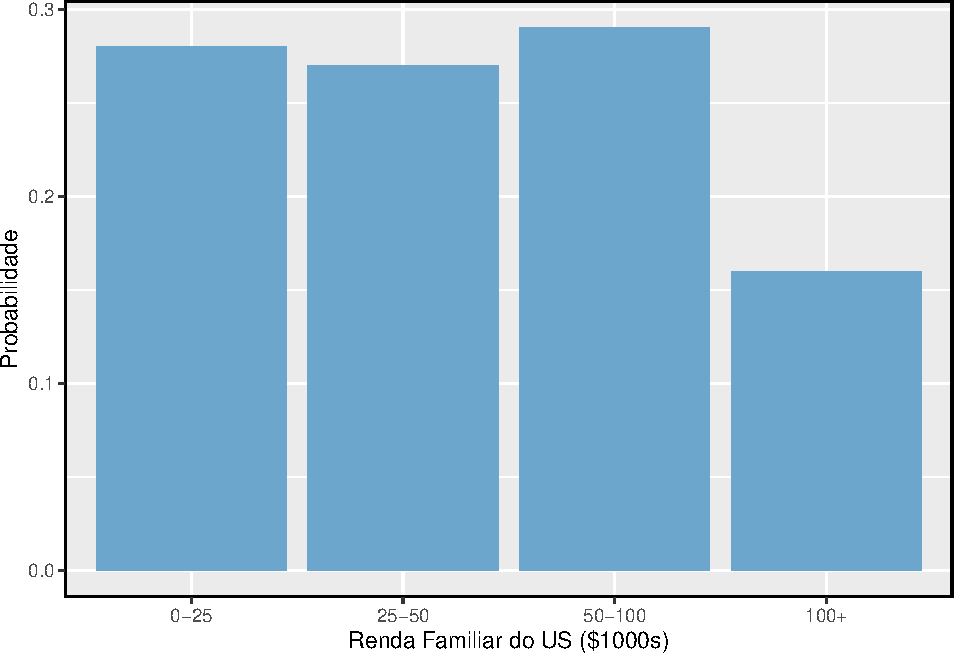
\includegraphics{_main_files/figure-latex/usHouseholdIncomeDistBar-1.pdf}
\caption{\label{fig:usHouseholdIncomeDistBar}A distribuição de probabilidade da renda familiar dos EUA.}
\end{figure}

\begin{figure}
\centering
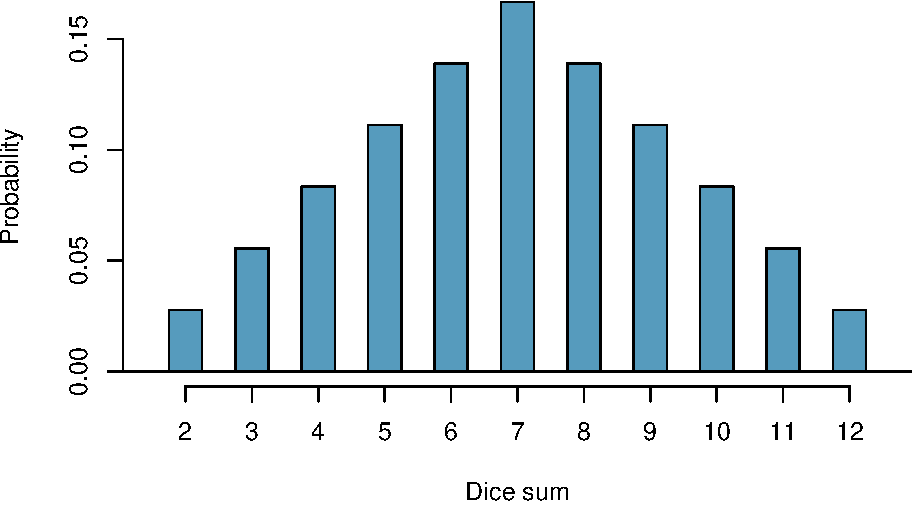
\includegraphics{_main_files/figure-latex/diceSumDist-1.pdf}
\caption{\label{fig:diceSumDist}A distribuição de probabilidade da soma de dois dados.}
\end{figure}

Nestas colunas de barras, as alturas das barras representam as probabilidades de resultados. Se os resultados forem numéricos e discretos, geralmente é (visualmente) conveniente fazer um gráfico de barras que se pareça com um histograma, como no caso da soma de dois dados. Outro exemplo de gráfico de barras em suas respectivas localizações é mostrado na Figura \ref{fig:bookCostDist}.

\hypertarget{complementEvent}{%
\subsection{Complemento de um evento}\label{complementEvent}}

Jogar um dado produz um valor no conjunto \(\{1, 2, 3, 4, 5, 6\}\). Esse conjunto de todos os resultados possíveis é chamado de \textbf{espaço amostral} (\(S\))

Vamos considerar que \(D=\{2, 3\}\) representa o evento que o resultado de um rolamento de dados é 2 ou 3. Então o \emph{complemento} do \(D\) representa todos os resultados em nosso espaço amostral que não estão em \(D\), que é denotado por \(D^c = \{1, 4, 5, 6\}\). Ou seja, \(D^c\) é o conjunto de todos os resultados ainda possíveis e não incluídos no \(D\). A Figura \ref{fig:complementOfD} mostra a relação entre \(D\), \(D^c\), e o espaço amostral \(S\).

\begin{figure}
\centering
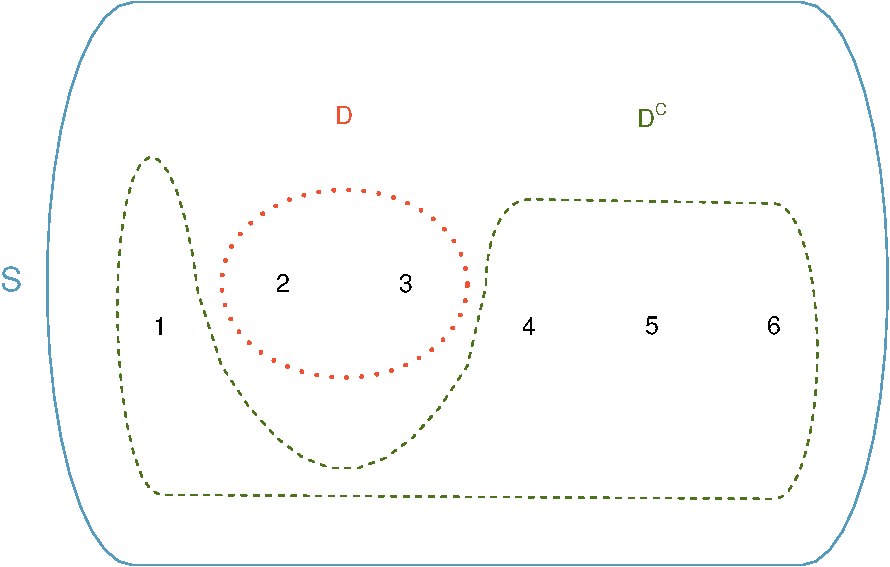
\includegraphics{_main_files/figure-latex/complementOfD-1.pdf}
\caption{\label{fig:complementOfD}Evento D = \{2, 3\} e seu complemento \{1, 4, 5, 6\}. S representa o espaço amostral, que é o conjunto de todos os resultados possíveis.}
\end{figure}

\begin{center}\rule{0.5\linewidth}{0.5pt}\end{center}

\begin{exercise}
\protect\hypertarget{exr:unnamed-chunk-51}{}{\label{exr:unnamed-chunk-51} }(a) Calcule \(P(D^c) = P(\text{lançar um} 1, 4, 5,\text{ ou }6)\).
(b) Qual é a \(P(D) + P(D^c)\)?\footnote{(a) Os resultados são disjuntos e cada um tem probabilidade \(1/6\), então a probabilidade total é \(4/6 = 2/3\). (b) Nós também podemos ver isso \(P(D)=\frac{1}{6} + \frac{1}{6} = 1/3\). Desde que \(D\) e \(D^c\) são disjuntos, \(P(D) + P(D^c) = 1\).}
\end{exercise}

\begin{center}\rule{0.5\linewidth}{0.5pt}\end{center}

\begin{center}\rule{0.5\linewidth}{0.5pt}\end{center}

\begin{exercise}
\protect\hypertarget{exr:unnamed-chunk-52}{}{\label{exr:unnamed-chunk-52} }Eventos \(A=\{1, 2, 4, 6\}\) são mostrados na Figura \ref{fig:disjointSets}.
(a) Escreva o que \(A^c\) e \(B^c\) representam.
(b)Calcule \(P(A^c)\) e \(P(B^c)\).
(c)Calcule \(P(A)+P(A^c)\) e \(P(B)+P(B^c)\).\footnote{Soluções breves: (a) \(A^c = \{3, 4, 5, 6\}\) e \(B^c=\{1,2,3,5\}\). (b) Observando que cada resultado é disjunto, adicione as probabilidades dos resultados individuais para obter \(P(A^c)=2/3\) e \(P(B^c)=2/3\). (c) \(A\) e \(A^c\) são disjuntos, e o mesmo vale para \(B\) e \(B^c\). Assim sendo, \(P(A) + P(A^c) = 1\) e \(P(B) + P(B^c) = 1\).}
\end{exercise}

\begin{center}\rule{0.5\linewidth}{0.5pt}\end{center}

Um complemento de um evento \(A\) é construído para ter duas propriedades muito importantes: (i) todo resultado possível não em \(A\) é em \(A^c\), e (ii) \(A\) e \(A^c\) são disjunto. Propriedade (i) implica

\begin{eqnarray}
P(A\text{ ou }A^c) = 1
\label{eq:complementSumTo1}
\end{eqnarray}

Isto é, se o resultado não estiver em \(A\), deve ser representado em \(A^c\). Usamos a regra da adição para eventos separados para aplicar a propriedade (ii):

\begin{eqnarray}
P(A\text{ ou }A^c) = P(A) + P(A^c)
\label{eq:complementDisjointEquation}
\end{eqnarray}

Combinando as Equações @ref(eq:complementSumTo1\} e \eqref{eq:complementDisjointEquation} rende uma relação muito útil entre a probabilidade de um evento e seu complemento.

Complemento O complemento do evento \(A\) é denotado por \(A^c\) e representa todos os resultados que não estão em\textasciitilde{} \(A\). \(A\) e \(A^c\) estão matematicamente relacionados:

\begin{eqnarray}
P(A) + P(A^c) = 1, \text{ i.e. } P(A) = 1-P(A^c)
\label{eq:complement}
\end{eqnarray}

Em exemplos simples, a computação de \(A\) ou \(A^c\) é viável em poucos passos. No entanto, usar o complemento pode economizar muito tempo à medida que os problemas aumentam em complexidade.

\begin{center}\rule{0.5\linewidth}{0.5pt}\end{center}

\begin{exercise}
\protect\hypertarget{exr:unnamed-chunk-53}{}{\label{exr:unnamed-chunk-53} }Vamos representar \(A\) o evento onde jogamos dois dados e o total deles é menor que 12.
(a) O que o evento \(A^c\) representa?
(b) Determine \(P(A^c)\) da Tabela \ref{tab:diceProb}.
(c) Determine \(P(A)\).\footnote{(a) O complemento de \(A\): quando o total é igual a 12. (b) \(P(A^c) = 1/36\). (c) Use a probabilidade do complemento da parte (b), \(P(A^c) = 1/36\), e Equação \eqref{eq:complement}: \(P(\text{menos do que }12) = 1 - P(12) = 1 - 1/36 = 35/36\).}
\end{exercise}

\begin{center}\rule{0.5\linewidth}{0.5pt}\end{center}

\begin{center}\rule{0.5\linewidth}{0.5pt}\end{center}

\begin{exercise}
\protect\hypertarget{exr:unnamed-chunk-54}{}{\label{exr:unnamed-chunk-54} }Considere novamente as probabilidades da Tabela \ref{tab:diceProb} e o jogar dois dados. Encontre as seguintes probabilidades:
(a) A soma dos dados \emph{não} é 6.
(b) A soma é pelo menos 4. Ou seja, determine a probabilidade do evento \(B=\{4, 5, \dots, 12\}\).
(c) A soma não é mais que 10. Ou seja, determine a probabilidade do evento \(D=\{2, 3, \dots, 10\}\).\footnote{(a) Primeiro ache \(P(6)=5/36\), então use o complemento: \(P(\text{não }6) = 1 - P(6) = 31/36\). (b) Primeiro, encontre o complemento, que requer muito menos esforço: \(P(2 \text{ ou } 3)=1/36+2/36=1/12\). Então calcule \(P(B) = 1-P(B^c) = 1-1/12 = 11/12\). (c) Como antes, encontrar o complemento é a maneira inteligente de determinar \(P(D)\). Primeiro ache \(P(D^c) = P(11 \text{ ou } 12)=2/36 + 1/36=1/12\). Então calcule \(P(D) = 1 - P(D^c) = 11/12\).}
\end{exercise}

\begin{center}\rule{0.5\linewidth}{0.5pt}\end{center}

\hypertarget{probabilityIndependence}{%
\subsection{Independência}\label{probabilityIndependence}}

Assim como variáveis e observações podem ser independentes, processos aleatórios podem ser independentes também. Dois processos são \textbf{independentes}, se conhecer o resultado de um não fornece informações úteis sobre o resultado do outro. Por exemplo, jogar uma moeda e jogar um dado são dois processos independentes -- saber que a moeda é cara não ajuda a determinar o resultado de um lançamento de dados. Por outro lado, os preços das ações geralmente sobem ou descem juntos, então eles não são independentes.

O Exemplo \ref{exm:probOf2Ones} fornece um exemplo básico de dois processos independentes: jogar dois dados. Queremos determinar a probabilidade de ambos serem 1. Suponha que um dos dados seja vermelho e o outro branco. Se o resultado do dado vermelho for 1, ele não fornece informações sobre o resultado do dado branco. Nós encontramos a mesma pergunta pela primeira vez no Exemplo \ref{exm:probOf2Ones}, onde calculamos a probabilidade usando o seguinte raciocínio: \(1/6\) das vezes o dado vermelho é um 1, e \(1/6\) dessas vezes o dado branco também será 1. Isso é ilustrado na Figura \ref{fig:indepForRollingTwo1s}. Como os testes são independentes, as probabilidades dos resultados correspondentes podem ser multiplicadas para obter a resposta final: \((1/6)\times(1/6)=1/36\). Isso pode ser generalizado para muitos processos independentes.

\begin{figure}
\centering
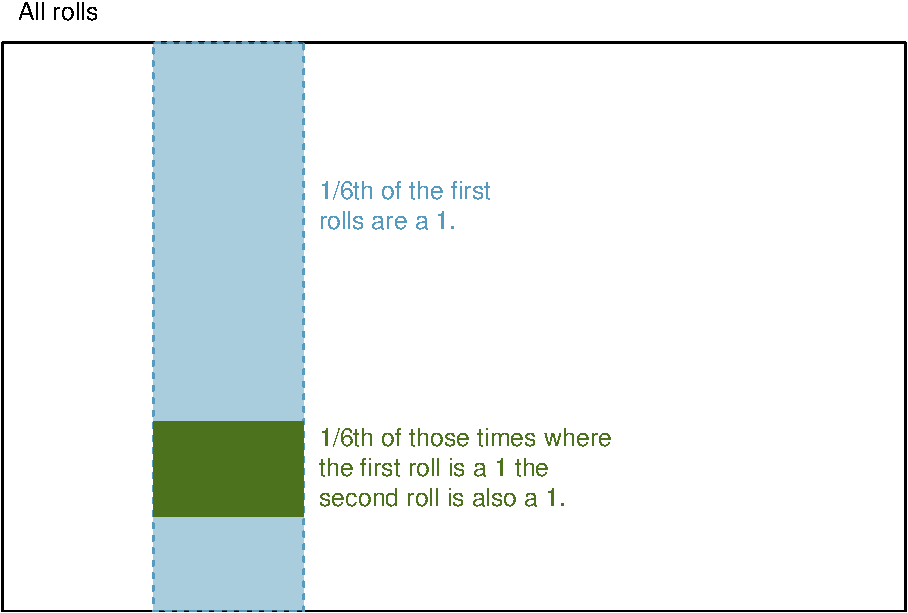
\includegraphics{_main_files/figure-latex/indepForRollingTwo1s-1.pdf}
\caption{\label{fig:indepForRollingTwo1s}1/6 das vezes, a primeira jogada é um 1. Então 1/6 dessas vezes, a segunda jogada também será um 1.}
\end{figure}

\begin{example}
\protect\hypertarget{exm:threeDice}{}{\label{exm:threeDice} }Se houvesse também um dado azul independente dos outros dois? Qual é a probabilidade de jogar os três dados e obter todos os 1s?
\end{example}

A mesma lógica se aplica a partir do Exemplo \ref{exm:probOf2Ones}. Se \(1/36\) das vezes os dados brancos e vermelhos são ambos 1, então \(1/6\) dessas vezes o dado azul também será 1, então multiplique:

\begin{align*}
P(\text{branco} = 1 \text{ e vermelho } = 1 \text{ e azul } = 1) \\
= P(\text{branco} = 1) \times P(\text{vermelho } = 1) \times P(\text{azul } = 1) \\
= 1/6 \times 1/6 \times 1/6 = 1/216.
\end{align*}

O Exemplo \ref{exm:threeDice} ilustra o que é chamado de Regra da Multiplicação para processos independentes,

Regra da Multiplicação para processos independentes Se \(A\) e \(B\) representam eventos de dois processos diferentes e independentes, então a probabilidade de ocorrer tanto \(A\) como \(B\) pode ser calculada como o produto de suas probabilidades separadas:

\begin{eqnarray}
P(A \text{ e }B) = P(A) \times  P(B)
\label{eq:eqForIndependentEvents}
\end{eqnarray}

Da mesma forma, se houver \(k\) eventos \(A_1,\dots, A_k\) de \(k\) processos independentes, então a probabilidade de que todos ocorram é

\begin{eqnarray*}
P(A_1) \times  P(A_2)\times  \cdots \times  P(A_k)
\end{eqnarray*}

\begin{center}\rule{0.5\linewidth}{0.5pt}\end{center}

\begin{exercise}
\protect\hypertarget{exr:ex2Handedness}{}{\label{exr:ex2Handedness} }Cerca de 9\% das pessoas são canhotas. Suponha que duas pessoas sejam selecionadas aleatoriamente da população dos EUA. Como o tamanho da amostra de 2 é muito pequeno em relação à população, é razoável supor que essas duas pessoas sejam independentes. (a) Qual é a probabilidade de ambos serem canhotos? (b) Qual é a probabilidade de ambos serem destros?\footnote{(a) A probabilidade da primeira pessoa ser canhota é de \(0,09\), o que é o mesmo para a segunda pessoa. Aplicamos a regra de multiplicação para processos independentes para determinar a probabilidade de ambos serem canhotos: \(0.09 \times 0.09 = 0.0081\). (b) É razoável supor que a proporção de pessoas que são ambidestras (tanto destros quanto canhotos) é quase 0, o que resulta em \(P(\text{destro}) = 1 - 0.09 = 0.91\). Usando o mesmo raciocínio como em parte (a), a probabilidade de ambos serem destros é \(0.91 \times 0.91 = 0.8281\).}
\end{exercise}

\begin{center}\rule{0.5\linewidth}{0.5pt}\end{center}

\begin{center}\rule{0.5\linewidth}{0.5pt}\end{center}

\begin{exercise}
\protect\hypertarget{exr:ex5Handedness}{}{\label{exr:ex5Handedness} }
Suponha que 5 pessoas sejam selecionadas aleatoriamente.\footnote{(a) As abreviações D e C são usadas para destros e canhotos, respectivamente. Como cada um é independente, aplicamos a regra de multiplicação para processos independentes: \(P(\text{todos são D}) = P(\text{primeiro} = D, \text{ segundo } = D, \dots, \text{ quinto } = D) = P(\text{primeiro } = D)\times P(\text{segundo} = D)\times \dots \times P(\text{quinto }= D) = 0.91\times 0.91\times 0.91\times 0.91\times 0.91 = 0.624\) (b) Usando o mesmo raciocínio que (a), \(0,09\times 0,09\times 0,09\times 0,09\times 0,09 = 0,0000059\). (c) Use o complemento, \(P(\text{todos os cinco são D})\), para responder a esta pergunta: \$P(\text{nem todos D}) = 1 - P(\text{todos D}) = 1 -- 0,624 = 0,376}\${]}
(a) Qual é a probabilidade de que todos sejam destros?
(b) Qual é a probabilidade de que todos sejam canhotos?
(c) Qual é a probabilidade de que nem todas as pessoas sejam destras?
\end{exercise}

\begin{center}\rule{0.5\linewidth}{0.5pt}\end{center}

Suponha que as variáveis \emph{servidão} e \emph{gênero} sejam independentes, ou seja, saber que o gênero de alguém não fornece informações úteis sobre a servidão e vice-versa. Então podemos calcular se uma pessoa selecionada aleatoriamente é destra e mulher\footnote{A proporção real da população dos EUA que é mulher é de aproximadamente 50\%, e então usamos 0.5 para a probabilidade de amostrar uma mulher. No entanto, essa probabilidade é diferente em outros países.}. Usando a regra de multiplicação:

\begin{eqnarray*}
P(\text{destro e mulher }) &=& P(\text{destro }) \times  P(\text{feminino}) \\
&=& 0,91 \times  0,50 = 0,455
\end{eqnarray*}

\begin{center}\rule{0.5\linewidth}{0.5pt}\end{center}

\begin{exercise}
\protect\hypertarget{exr:unnamed-chunk-55}{}{\label{exr:unnamed-chunk-55} }
Três pessoas são selecionadas aleatoriamente.\footnote{Breves respostas são fornecidas. (a) Isso pode ser escrito em notação de probabilidade como \(P(\text{a pessoa selecionada aleatoriamente é do sexo masculino e destro}) = 0.455\). (b) 0.207. (c) 0.045. (d) 0.0093.}
(a) Qual é a probabilidade de que a primeira pessoa seja do sexo masculino e destro?
(b) Qual é a probabilidade de que as duas primeiras pessoas sejam do sexo masculino e destras ?
(c) Qual é a probabilidade de que a terceira pessoa seja do sexo feminino e canhoto?
(d) Qual é a probabilidade de que as duas primeiras pessoas sejam do sexo masculino e destras e a terceira pessoa seja do sexo feminino e canhoto?
\end{exercise}

\begin{center}\rule{0.5\linewidth}{0.5pt}\end{center}

Às vezes nos perguntamos se um resultado fornece informações úteis sobre outro resultado. A pergunta que estamos fazendo é: as ocorrências dos dois eventos são independentes? Dizemos que dois eventos \(A\) e \(B\) são independentes se satisfizerem a Equação \eqref{eq:eqForIndependentEvents}.

\begin{example}
\protect\hypertarget{exm:unnamed-chunk-56}{}{\label{exm:unnamed-chunk-56} }Se embaralharmos um baralho de cartas e pegarmos uma carta, o evento que a carta é de copas é independente do evento em que o carta é um ás? A probabilidade de a carta ser de copas é de \(1/4\) e a probabilidade de ser um ás é \(1/13\). A probabilidade da carta ser o ás de copas é \(1/52\). Nós verificamos se a Equação \eqref{eq:eqForIndependentEvents} é satisfeita:
\end{example}

\begin{align*}
P({\heartsuit})\times P(\text{ás}) = \frac{1}{4}\times \frac{1}{13} = \frac{1}{52} 
                    = P({\heartsuit}\text{ e ás})
\end{align*}

Porque a equação é válida, o evento em que a carta é de copas e o evento em que a carta é um ás são eventos independentes.

\hypertarget{conditionalProbabilitySection}{%
\section{Probabilidade condicional (tópico especial)}\label{conditionalProbabilitySection}}

O conjunto de dados \texttt{família\_ensino} contém uma amostra de 792 casos com duas variáveis, \emph{adolescentes} e \emph{pais}, e está resumido na Tabela \ref{tab:contTableOfParStCollege}.\footnote{Um conjunto de dados simulado baseado em resumos reais da população em nces.ed.gov/pubs2001/2001126.pdf.} A variável adolescentes é: \emph{faculdade} ou \emph{não}, onde o rótulo faculdade significa que o adolescente foi para a faculdade imediatamente após o ensino médio. A variável pais recebe o valor \emph{graduado} se pelo menos um dos pais do adolescente tiver completado o ensino superior.

\begin{table}

\caption{\label{tab:contTableOfParStCollege}Tabela de contingência resumindo o conjunto de dados familia ensino}
\centering
\begin{tabular}[t]{l|c|c|c}
\hline
  & graduado & não & total\\
\hline
faculdade & 231 & 214 & 445\\
\hline
não & 49 & 298 & 347\\
\hline
total & 280 & 512 & 792\\
\hline
\end{tabular}
\end{table}

\begin{figure}
\centering
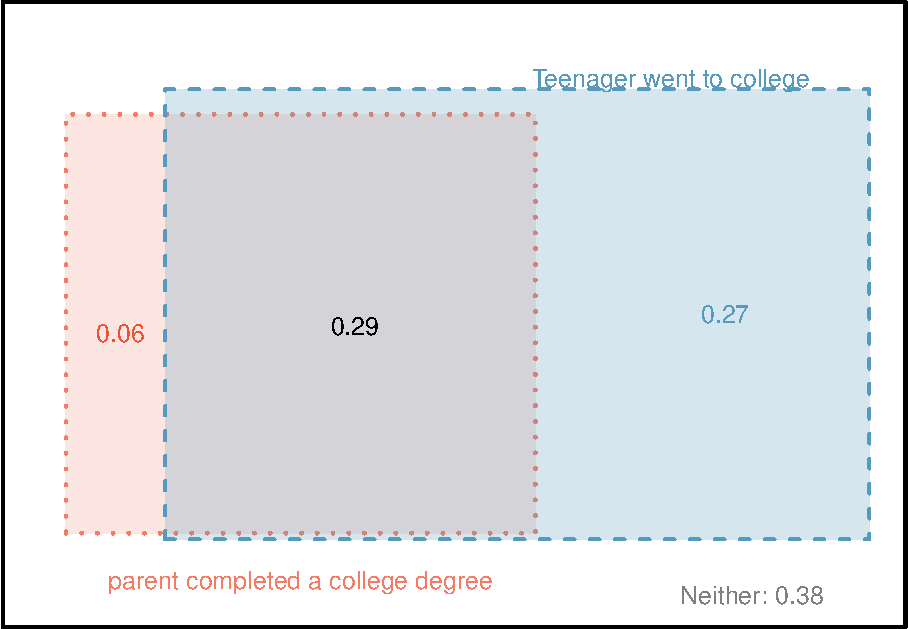
\includegraphics{_main_files/figure-latex/familyCollegeVenn-1.pdf}
\caption{\label{fig:familyCollegeVenn}Um diagrama de Venn usando caixas para o conjunto de dados familia\_ensino}
\end{figure}

\begin{example}
\protect\hypertarget{exm:unnamed-chunk-57}{}{\label{exm:unnamed-chunk-57} }Se pelo menos um dos pais de um adolescente concluiu o curso superior, qual é a chance de o adolescente frequentar a faculdade logo após o ensino médio?
\end{example}

Podemos estimar essa probabilidade usando os dados. Dos 280 casos neste conjunto de dados onde \emph{pais} leva valor \emph{graduado}, 231 representam casos em que a variável \emph{adolescente} leva valor \emph{faculdade}:

\begin{eqnarray*}
P(\text{adolescente faculdade | pais graduado}) = \frac{231}{280} = 0.825
\end{eqnarray*}

\begin{example}
\protect\hypertarget{exm:collegeProbOfParentsGivenStudentNot}{}{\label{exm:collegeProbOfParentsGivenStudentNot} }Uma adolescente é selecionada aleatoriamente da amostra e ela não frequentou a faculdade logo após o ensino médio. Qual é a probabilidade de que pelo menos um dos pais dela tenha um diploma universitário?
\end{example}

Se a adolescente não frequentou a faculdade logo após o ensino médio, ela é uma das 347 adolescentes da segunda fila. Dos 347 adolescentes, 49 tiveram pelo menos um dos pais que obteve um diploma universitário:

\begin{eqnarray*}
P(\text{pais graduado | adolescente não}) = \frac{49}{347} = 0.141
\end{eqnarray*}

\hypertarget{marginalAndJointProbabilities}{%
\subsection{Probabilidades marginais e conjuntas}\label{marginalAndJointProbabilities}}

A Tabela \ref{tab:contTableOfParStCollege} inclui totais de linha e coluna para cada variável separadamente no conjunto de dados \texttt{faculdade\_família}. Esses totais representam \textbf{probabilidades marginais} para a amostra, que são as probabilidades baseadas em uma única variável sem considerar quaisquer outras variáveis. Por exemplo, uma probabilidade baseada apenas na variável adolescente é uma probabilidade marginal:

\begin{align*}
P(\text{adolescente faculdade}) = \frac{445}{792} = 0.56
\end{align*}

Uma probabilidade de resultados para duas ou mais variáveis ou processos é chamada de \textbf{probabilidade conjunta}:

\begin{align*}
P(\text{adolescente faculdade e pais não}) = \frac{214}{792} = 0.27
\end{align*}

É comum substituir uma vírgula por ``e'\,' em uma probabilidade conjunta, embora seja aceitável. Isso é,

\[
P(\text{adolescente faculdade, pais não}) = P(\text{adolescente faculdade e pais não})
\]

Probabilidades marginais e conjuntas: Se uma probabilidade é baseada em uma única variável, é uma \textbf{probabilidade marginal}. A probabilidade de resultados para duas ou mais variáveis ou processos é chamada de \textbf{probabilidade conjunta}.

Nós usamos \emph{tabelas de proporções} para resumir as probabilidades conjuntas para a amostra \texttt{faculdade\textbackslash{}\_família}. Essas proporções são calculadas dividindo cada contagem na Tabela \ref{tab:contTableOfParStCollege} pelo total da tabela, 792, para obter as proporções na Tabela \ref{tab:familyCollegeProbTable}. A distribuição de probabilidade conjunta das variáveis pais e adolescentes é mostrada na Tabela \ref{tab:familyCollegeDistribution}.

\begin{table}

\caption{\label{tab:familyCollegeProbTable}Tabela de probabilidade resumindo se pelo menos um dos pais tinha um diploma universitário e se o adolescente frequentou a faculdade.}
\centering
\begin{tabular}[t]{l|c|c|c}
\hline
  & pais:graduado & pais:não & Total\\
\hline
adolescente:faculdade & 0.29 & 0.27 & 0.56\\
\hline
adolescente:não & 0.06 & 0.38 & 0.44\\
\hline
Total & 0.35 & 0.65 & 1.00\\
\hline
\end{tabular}
\end{table}

\begin{table}

\caption{\label{tab:familyCollegeDistribution}Distribuição de probabilidade conjunta para o conjunto de dados faculdade familia}
\centering
\begin{tabular}[t]{c|c}
\hline
Resultado Conjunto & Probabilidade\\
\hline
pais:graduado e adolescente:faculdade & 0.29\\
\hline
pais:graduado e adolescente:não & 0.06\\
\hline
pais:não e adolescente:faculdade & 0.27\\
\hline
pais:não e adolescente:não & 0.38\\
\hline
Total & 1\\
\hline
\end{tabular}
\end{table}

\begin{center}\rule{0.5\linewidth}{0.5pt}\end{center}

\begin{exercise}
\protect\hypertarget{exr:unnamed-chunk-58}{}{\label{exr:unnamed-chunk-58} }Verifique que a Tabela \ref{tab:familyCollegeDistribution} representa uma distribuição de probabilidade: os eventos são separados, todas as probabilidades são não-negativas e as probabilidades somam 1.\footnote{Cada uma das quatro combinações de resultados é disjunta, todas as probabilidades são de fato não-negativas e a soma das probabilidades é \$0.29 + 0.06 + 0.27 + 0.38 = 1.00 \$.}
\end{exercise}

\begin{center}\rule{0.5\linewidth}{0.5pt}\end{center}

Podemos calcular as probabilidades marginais usando probabilidades conjuntas em casos simples. Por exemplo, a probabilidade de um adolescente aleatório do estudo ir para a faculdade é encontrada somando os resultados onde adolescente leva o valor faculdade:

\begin{align*}
P(\text{adolescente faculdade})
&=  P(\text{pais graduado e adolescente faculdade}) + P(\text{pais não e adolescente faculdade}) \\
&= 0.29 + 0.27 \\
&= 0.56
\end{align*}

\hypertarget{definingConditionalProbability}{%
\subsection{Definindo probabilidade condicional}\label{definingConditionalProbability}}

Há alguma conexão entre o nível de escolaridade dos pais e do adolescente: um diploma universitário de um dos pais está associado com a decisão de ir para uma faculdade do adolescente. Nesta seção, discutiremos como usar informações sobre associações entre duas variáveis para melhorar a estimativa de probabilidade.

A probabilidade de um adolescente aleatório do estudo freqüentar a faculdade é de 0,56. Poderíamos atualizar essa probabilidade se soubéssemos que um dos pais do adolescente tem um diploma universitário? Absolutamente. Para fazer isso, limitamos nossa visão apenas aos 280 casos em que um pai tem um diploma universitário e olha a fração em que o adolescente frequentou a faculdade:

\begin{eqnarray*}
P(\text{adolescente faculdade | pais graduado}) = \frac{231}{280} = 0.825
\end{eqnarray*}

Chamamos isso de \textbf{probabilidade condicional} porque calculamos a probabilidade sob uma condição: um pai tem um diploma universitário. Existem duas partes para uma probabilidade condicional, o \emph{termo de interesse} e a \emph{condição}. É útil pensar na condição como informação que sabemos ser verdadeira, e essa informação geralmente pode ser descrita como um resultado ou evento conhecido.

Nós separamos o texto dentro de nossa notação de probabilidade no resultado de interesse e a condição\footnote{A barra vertical ``\(|\)'\,' é lida como \emph{dado}.}:

\begin{eqnarray}
&& P(\text{adolescente faculdade | pais graduado})  \\
&& = P(\text{adolescente faculdade}\ |\ \text{pais graduado}) = \frac{231}{280} = 0.825
\label{eq:probStudentUsedIfParentsUsedInFormalNotation}
\end{eqnarray}

Na Equação \eqref{eq:probStudentUsedIfParentsUsedInFormalNotation}, calculamos a probabilidade de um adolescente frequentar a faculdade com base na condição de que pelo menos um dos pais tenha um diploma universitário como uma fração:

\begin{eqnarray}
&& P(\text{adolescente faculdade} | \text{pais graduado}) \\
&&\quad = \frac{\text{\# casos onde adolescente faculdade e pais graduado}}{\text{\# casos onde pais graduado}} \\
&&\quad = \frac{231}{280} = 0.825 \notag
\label{eq:ratioOfBothToRatioOfConditionalForParentsAndStudent}
\end{eqnarray}

Consideramos apenas os casos que preenchiam a condição, \emph{pais graduado} e, em seguida, calculamos a proporção dos casos que satisfizeram nosso resultado de interesse, o adolescente cursou a faculdade.

Frequentemente, probabilidades marginais e conjuntas são fornecidas em vez de dados de contagem. Por exemplo, as taxas de doenças são comumente listadas em porcentagens, e não em um formato de contagem. Gostaríamos de poder computar probabilidades condicionais mesmo quando não há contagens disponíveis, e usamos a Equação\eqref{eq:ratioOfBothToRatioOfConditionalForParentsAndStudent} como um modelo para entender essa técnica.

Consideramos apenas os casos que satisfizeram a condição, \emph{pais graduado}. Destes casos, a probabilidade condicional foi a fração que representou o desfecho de interesse, \emph{adolescente faculdade}. Suponha que nos foram fornecidas apenas as informações na Tabela \ref{tab:familyCollegeProbTable}, isto é, apenas dados de probabilidade. Então, se pegássemos uma amostra de 1000 pessoas, anteciparíamos cerca de 35\% ou \(0.35\times 1000 = 350\) satisfariam o critério de informação (pais graduado). Da mesma forma, seria de esperar cerca de 29\% ou \(0.29\times 1000 = 290\) para atender aos critérios de informação e representar nosso resultado de interesse. Então a probabilidade condicional pode ser computada como:

\begin{align}
&P(\text{adolescente faculdade} | \text{pais graduado})  \\
    &= \frac{\text{\# (adolescente faculdade e pais graduado)}}{\text{\# (pais graduado)}}  \\
    &= \frac{290}{350}
        = \frac{0.29}{0.35}
        = 0.829\quad\text{( diferente de 0.825 devido a erro de arredondamento)}
\label{eq:stUserPUsedHypSampSize}
\end{align}

Na Equação \eqref{eq:stUserPUsedHypSampSize}, nós examinamos exatamente a fração de duas probabilidades, 0.29 e 0.35, que podemos escrever como

\begin{align*}
P(\text{adolescente faculdade e pais graduado})
    \quad\text{e}\quad
    P(\text{pais graduado}).
\end{align*}

A fração dessas probabilidades é um exemplo da fórmula geral para probabilidade condicional.

Probabilidade condicional: A probabilidade condicional do resultado do evento \(A\) dada condição \(B\) é calculada como o seguinte:

\begin{align}
P(A | B) = \frac{P(A\text{ e }B)}{P(B)}
\label{eq:condProbEq}
\end{align}

\begin{center}\rule{0.5\linewidth}{0.5pt}\end{center}

\begin{exercise}
\protect\hypertarget{exr:familyCollegeProbOfParentsEqualNotGivenTeen}{}{\label{exr:familyCollegeProbOfParentsEqualNotGivenTeen} }(a) Escreva a seguinte declaração em notação de probabilidade condicional: \textbf{A probabilidade de um caso aleatório em que nenhum dos pais tem um diploma universitário, se é sabido que o adolescente não frequentou a faculdade logo após o ensino médio}. Observe que a condição agora é baseada no adolescente, não nos pais.
(b) Determinar a probabilidade de parte (a). A Tabela \ref{tab:familyCollegeProbTable} pode ser útil.\footnote{(a) \(P(\text{pais não}\ | \text{adolescente não})\). (b) Equação \eqref{eq:condProbEq} para probabilidade condicional indica que devemos primeiro encontrar \(P(\text{pais não e adolescente não}) = 0.38\) e \(P(\text{adolescente não}) = 0.44\). Então a proporção representa a probabilidade condicional: \(0.38 / 0.44 = 0.864\).}
\end{exercise}

\begin{center}\rule{0.5\linewidth}{0.5pt}\end{center}

\begin{center}\rule{0.5\linewidth}{0.5pt}\end{center}

\begin{exercise}
\protect\hypertarget{exr:whyCondProbSumTo1}{}{\label{exr:whyCondProbSumTo1} }(a) Determinar a probabilidade de um dos pais ter um diploma universitário, se se sabe que o adolescente não frequentou a faculdade.
(b) Usando as respostas da parte (a) e Prática Orientada \ref{exr:familyCollegeProbOfParentsEqualNotGivenTeen} (b), calcule \(P(\text{pais graduado | adolescente não}) + P(\text{pais não | adolescente não})\)
(c) Forneça um argumento intuitivo para explicar por que a soma de (b) é 1.\footnote{(a) Esta probabilidade é \(\frac{P(\text{pais graduado, adolescente não})}{P(\text{adolescente não})} = \frac{0.06}{0.44} = 0.136\). (b) O total é igual a 1. (c) Sob a condição de o adolescente não frequentar a faculdade, os pais devem ter um diploma universitário ou não. O complemento ainda funciona para probabilidades condicionais, desde que as probabilidades estejam condicionadas à mesma informação.}
\end{exercise}

\begin{center}\rule{0.5\linewidth}{0.5pt}\end{center}

\begin{center}\rule{0.5\linewidth}{0.5pt}\end{center}

\begin{exercise}
\protect\hypertarget{exr:unnamed-chunk-59}{}{\label{exr:unnamed-chunk-59} }Os dados indicam que há uma associação entre os pais que possuem um diploma universitário e o adolescente que frequenta a faculdade. Isso significa que o(s) grau(s) universitário(s) dos pais causou o adolescente a ir para a faculdade?\footnote{Não. Embora haja uma associação, os dados são observacionais. Duas variáveis potencialmente confundidoras incluem renda e região. Você pode pensar nas outras.}
\end{exercise}

\begin{center}\rule{0.5\linewidth}{0.5pt}\end{center}

\hypertarget{boston1721}{%
\subsection{Varíola em Boston, 1721}\label{boston1721}}

O conjunto de dados \texttt{varíola} fornece uma amostra de 6.224 pessoas a partir do ano de 1721 que foram expostas à varíola em Boston.\footnote{Fenner F. 1988. \emph{Varíola e sua erradicação (História da Saúde Pública Internacional, nº 6)}. Genebra: Organização Mundial de Saúde. ISBN 92-4-156110-6.} Os médicos da época acreditavam que a inoculação, que envolve a exposição de uma pessoa à doença de forma controlada, poderia reduzir a probabilidade de morte.

Cada caso representa uma pessoa com duas variáveis: \emph{inoculada} e \emph{resultado.} A variável inoculada leva dois níveis: sim ou não, indicando se a pessoa foi inoculada ou não. A variável resultado tem resultados viveu ou morreu. Estes dados estão resumidos nas Tabelas \ref{tab:smallpoxContingencyTable} e \ref{tab:smallpoxProbabilityTable}.

\begin{table}

\caption{\label{tab:smallpoxContingencyTable}Tabela de contingência para o conjunto de dados varíola}
\centering
\begin{tabular}[t]{l|c|c|c}
\hline
  & inoculado: sim & inoculado: não & Total\\
\hline
resultado: viveu & 238 & 5136 & 5374\\
\hline
resultado: morreu & 6 & 844 & 850\\
\hline
Total & 244 & 5980 & 6224\\
\hline
\end{tabular}
\end{table}

\begin{table}

\caption{\label{tab:smallpoxProbabilityTable}Proporções da tabela para os dados de varíola, calculados dividindo cada contagem pelo total da tabela, 6224.}
\centering
\begin{tabular}[t]{l|c|c|c}
\hline
  & inoculado: sim & inoculado: não & Total\\
\hline
resultado: viveu & 0.0382 & 0.8252 & 0.8634\\
\hline
resultado: morreu & 0.0010 & 0.1356 & 0.1366\\
\hline
Total & 0.0392 & 0.9608 & 1.0000\\
\hline
\end{tabular}
\end{table}

\begin{center}\rule{0.5\linewidth}{0.5pt}\end{center}

\begin{exercise}
\protect\hypertarget{exr:probDiedIfNotInoculated}{}{\label{exr:probDiedIfNotInoculated} }Escreva, em notação formal, a probabilidade de uma pessoa selecionada aleatoriamente, que não foi inoculada, morrer de varíola, e calcule o valor da probabilidade.\footnote{\(P(\text{resultado} = \text{morreu} | \text{inoculado} = \text{não}) = \frac{P(\text{resultado = morreu e inoculado = não})}{P(\text{inoculado = não})} = \frac{0,1356}{0,9608} = 0,1411\).}
\end{exercise}

\begin{center}\rule{0.5\linewidth}{0.5pt}\end{center}

\begin{center}\rule{0.5\linewidth}{0.5pt}\end{center}

\begin{exercise}
\protect\hypertarget{exr:unnamed-chunk-60}{}{\label{exr:unnamed-chunk-60} }Determine a probabilidade de que uma pessoa inoculada tenha morrido de varíola. Como este resultado se compara com o resultado da Prática Orientada \ref{exr:probDiedIfNotInoculated}?\footnote{\(P(\text{resultado = morreu | inoculado = sim}) = \frac{P(\text{resultado = morreu e inoculado = sim})}{P(\text{inoculado = sim})} = \frac{0.0010}{0.0392} = 0.0255\) (se evitássemos erros de arredondamento, teríamos \(6 / 244 = 0.0246\)). A taxa de mortalidade para os indivíduos que foram inoculados é de apenas cerca de 1 em 40, enquanto a taxa de mortalidade é de cerca de 1 em 7 para aqueles que não foram inoculados.}
\end{exercise}

\begin{center}\rule{0.5\linewidth}{0.5pt}\end{center}

\begin{center}\rule{0.5\linewidth}{0.5pt}\end{center}

\begin{exercise}
\protect\hypertarget{exr:SmallpoxInoculationObsExpExercise}{}{\label{exr:SmallpoxInoculationObsExpExercise} }As pessoas de Boston se auto-selecionaram se deveriam ou não ser inoculadas.
(a) Este estudo é observacional ou foi uma experiência?
(b) Podemos inferir qualquer conexão causal usando esses dados?
(c) Quais são algumas possíveis variáveis de confusão que podem influenciar se alguém viveu ou morreu e também afeta se essa pessoa foi inoculada?\footnote{Respostas breves: (a) Observacional (b) Não, não podemos inferir a causalidade a partir deste estudo observacional. (c) Acessibilidade aos cuidados médicos mais recentes e melhores. Existem outras respostas válidas.}
\end{exercise}

\begin{center}\rule{0.5\linewidth}{0.5pt}\end{center}

\hypertarget{generalRuleMultiplication}{%
\subsection{Regra geral da multiplicação}\label{generalRuleMultiplication}}

Seção \ref{probabilityIndependence} introduziu a regra da multiplicação para processos independentes. Aqui nós fornecemos a \textbf{Regra Geral de Multiplicação} para eventos que podem não ser independentes.

Regra Geral de Multiplicação: Se \(A\) e \(B\) representam dois resultados ou eventos, então

\begin{eqnarray*}
P(A\text{ e }B) = P(A | B)\times P(B)
\end{eqnarray*}

É útil pensar em \(A\) como resultado de interesse e \(B\) como condição.

Esta Regra Geral de Multiplicação é simplesmente um rearranjo da definição de probabilidade condicional na Equação \eqref{eq:condProbEq}.

\begin{example}
\protect\hypertarget{exm:unnamed-chunk-61}{}{\label{exm:unnamed-chunk-61} }Considere o conjunto de dados varíola. Suponha que nos sejam dadas apenas duas informações: 96,08\% dos residentes não foram inoculados e 85,88\% dos residentes que não foram inoculados acabaram por sobreviver. Como poderíamos calcular a probabilidade de um residente não ter sido inoculado e vivido?

Nós calcularemos nossa resposta usando a regra de multiplicação geral e, em seguida, verificá-la usando Tabela \ref{tab:smallpoxProbabilityTable}. Queremos determinar

\begin{eqnarray*}
P(\text{resultado = viveu e inoculado = não})
\end{eqnarray*}

e nos é dado que

\begin{eqnarray*}
P(\text{resultado = viveu | inoculado = não})=0,8588 \\
P(\text{inoculado = não})=0,9608
\end{eqnarray*}

Entre os 96,08\% de pessoas que não foram inoculadas, 85,88\% sobreviveram:

\begin{eqnarray*}
P(\text{resultado = viveu e inoculado = não}) = 0,8588 \times 0,9608 = 0,8251
\end{eqnarray*}

Isso é equivalente à regra geral de multiplicação. Podemos confirmar essa probabilidade na Tabela \ref{tab:smallpoxProbabilityTable} na intersecção de não e viveu (com um pequeno erro de arredondamento).
\end{example}

\begin{center}\rule{0.5\linewidth}{0.5pt}\end{center}

\begin{exercise}
\protect\hypertarget{exr:unnamed-chunk-62}{}{\label{exr:unnamed-chunk-62} }Use \(P(inoculado = sim) = 0,0392\) e \(P(resultado = viveu | inoculado = sim) = 0,9754\) para determinar a probabilidade de que uma pessoa foi inoculada e viveu.\footnote{A resposta é 0´.0382, que pode ser verificada usando a Tabela \ref{tab:smallpoxProbabilityTable}.}
\end{exercise}

\begin{center}\rule{0.5\linewidth}{0.5pt}\end{center}

\begin{center}\rule{0.5\linewidth}{0.5pt}\end{center}

\begin{exercise}
\protect\hypertarget{exr:unnamed-chunk-63}{}{\label{exr:unnamed-chunk-63} }Se 97,54\% das pessoas que foram inoculadas viveram, que proporção de pessoas inoculadas deve ter morrido?\footnote{Houve apenas dois resultados possíveis: viveu ou morreu. Isso significa que 100\% - 97.54\% = 2.46\% das pessoas que foram inoculadas morreram.}
\end{exercise}

\begin{center}\rule{0.5\linewidth}{0.5pt}\end{center}

Soma das probabilidades condicionais: Vamos representar \(A_1, \dots, A_k\) todos os resultados disjuntos para uma variável ou processo. Então, se \(B\) é um evento, possivelmente para outra variável ou processo, temos:

\begin{eqnarray*}
P(A_1|B)+\cdots+P(A_k|B) = 1
\end{eqnarray*}

A regra para complementos também é válida quando um evento e seu complemento são condicionados à mesma informação:

\begin{eqnarray*}
P(A | B) = 1 - P(A^c | B)
\end{eqnarray*}

\begin{center}\rule{0.5\linewidth}{0.5pt}\end{center}

\begin{exercise}
\protect\hypertarget{exr:unnamed-chunk-64}{}{\label{exr:unnamed-chunk-64} }Com base nas probabilidades calculadas acima, parece que a inoculação é eficaz na redução do risco de morte por varíola?\footnote{As amostras são grandes em relação à diferença nas taxas de mortalidade para as inoculações \emph{inoculadas} e \emph{não inoculadas}, então parece que existe uma associação entre inoculado e resultado. No entanto, como observado na solução para Prática Orientada \ref{exr:SmallpoxInoculationObsExpExercise}, este é um estudo observacional e não podemos ter certeza se existe uma conexão causal. (Pesquisas adicionais mostraram que a inoculação é eficaz na redução das taxas de mortalidade.)}
\end{exercise}

\begin{center}\rule{0.5\linewidth}{0.5pt}\end{center}

\hypertarget{indConsiderationsCondProb}{%
\subsection{Considerações de independência em probabilidade condicional}\label{indConsiderationsCondProb}}

Se dois eventos são independentes, saber o resultado de um não deve fornecer informações sobre o outro. Nós podemos mostrar que isso é matematicamente verdadeiro usando probabilidades condicionais.

\begin{center}\rule{0.5\linewidth}{0.5pt}\end{center}

\begin{exercise}
\protect\hypertarget{exr:condProbOfRollingA1AfterOne1}{}{\label{exr:condProbOfRollingA1AfterOne1} }Vamos representar \(X\) e \(Y\) como resultados de jogar dois dados.\footnote{Soluções breves: (a) \(1/6\). (b) \(1/36\). (c) \(\frac{P(Y = \text{ 1 e }X=\text{ 1})}{P(X=\text{ 1})} = \frac{1/36}{1/6} = 1/6\). (d) A probabilidade é a mesma que na parte (c): \(P(Y=1)=1/6\). A probabilidade de que \(Y=1\) permaneceu inalterado pelo conhecimento sobre \(X\), o que faz sentido, pois \(X\) e \(Y\) são independentes.}
(a) Qual é a probabilidade de que \(X\) seja 1?
(b) Qual é a probabilidade de que tanto \(X\) quanto \(Y\) sejam 1?
(c) Use a fórmula para probabilidade condicional para calcular \(P(Y = 1\ | X = 1)\).
(d) O que é \(P(Y=1)\)? Isso é diferente da resposta da parte (c)? Explique.
\end{exercise}

\begin{center}\rule{0.5\linewidth}{0.5pt}\end{center}

Podemos mostrar na Prática Orientada \ref{exr:condProbOfRollingA1AfterOne1}(c) que a informação de condicionamento não tem influência usando a Regra de Multiplicação para processos independentes:

\begin{eqnarray*}
P(Y=\text{1}\ |\ X=\text{1})
    &=& \frac{P(Y=\text{1 e }X=\text{1})}{P(X=\text{1})} \\
    &=& \frac{P(Y=\text{1})\times P(X=\text{1})}{P(X=\text{1})} \\
    &=& P(Y=\text{1}) \\
\end{eqnarray*}

\begin{center}\rule{0.5\linewidth}{0.5pt}\end{center}

\begin{exercise}
\protect\hypertarget{exr:unnamed-chunk-65}{}{\label{exr:unnamed-chunk-65} }Ron está assistindo a uma mesa de roleta em um cassino e percebe que os últimos cinco resultados foram \emph{preto}. Ele acha que as chances de conseguir \emph{preto} seis vezes seguidas é muito pequena (cerca de \(1/64\)) e coloca seu salário em vermelho. O que está errado com seu raciocínio?\footnote{Ele esqueceu que o próximo giro da roleta é independente das rodadas anteriores. Casinos empregam esta prática; eles publicam os últimos resultados de muitos jogos de apostas para enganar os jogadores desavisados a acreditar que as probabilidades estão a seu favor. Isso é chamado de \textbf{falácia do jogador}.}
\end{exercise}

\begin{center}\rule{0.5\linewidth}{0.5pt}\end{center}

\hypertarget{treeDiagram}{%
\subsection{Diagramas de árvore}\label{treeDiagram}}

\textbf{Diagramas de árvore} são uma ferramenta para organizar resultados e probabilidades em torno da estrutura dos dados. Eles são mais úteis quando dois ou mais processos ocorrem em uma sequência e cada processo é condicionado em seus predecessores.

O \texttt{varíola} se encaixa nessa descrição. Nós vemos a população dividida por inoculação: sim e não. Após esta divisão, as taxas de sobrevivência foram observadas para cada grupo. Essa estrutura é refletida no \textbf{diagrama de árvore} mostrado na Figura \ref{fig:smallpoxTreeDiagram}. O primeiro ramo para inoculação é dito ser o ramo \emph{primário} enquanto os outros ramos são \emph{secundários}.

\begin{figure}
\centering
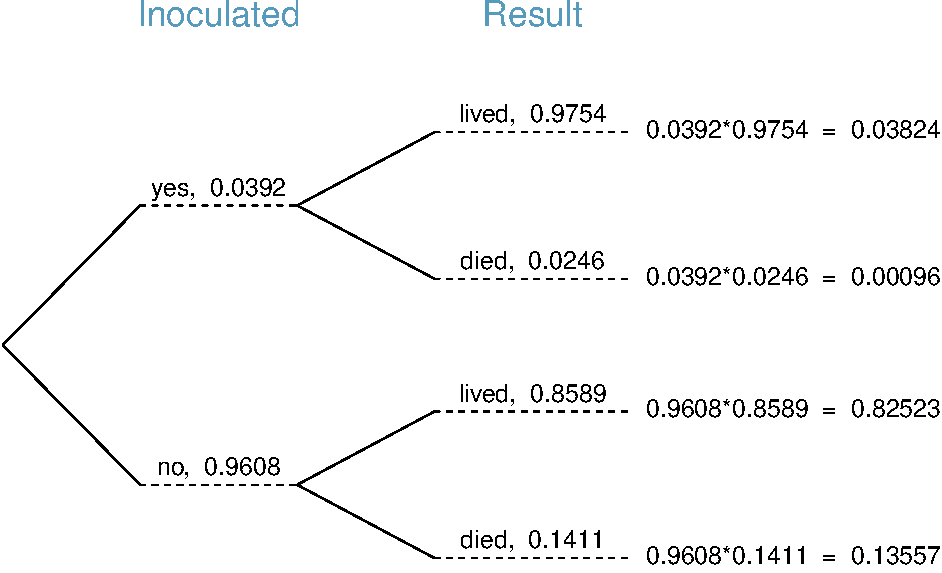
\includegraphics{_main_files/figure-latex/smallpoxTreeDiagram-1.pdf}
\caption{\label{fig:smallpoxTreeDiagram}Um diagrama de árvore do conjunto de dados varíola}
\end{figure}

Os diagramas de árvore são anotados com probabilidades marginais e condicionais, como mostrado na Figura \ref{fig:smallpoxTreeDiagram}. Este diagrama de árvore divide os dados de varíola por inoculação nos grupos sim e não com respectivas probabilidades marginais de 0.0392 e 0.9608. As ramificações secundárias são condicionadas na primeira, portanto, atribuímos probabilidades condicionais a essas ramificações. Por exemplo, o ramo superior na Figura \ref{fig:smallpoxTreeDiagram} é a probabilidade de que \texttt{resultado\ =\ viveu} condicionado à informação de que \texttt{inoculado\ =\ sim}. Podemos (e geralmente) construir probabilidades conjuntas no final de cada ramo em nossa árvore, multiplicando os números que encontramos enquanto nos movemos da esquerda para a direita. Estas probabilidades conjuntas são calculadas usando a Regra Geral de Multiplicação:

\begin{eqnarray*}
&& P(\text{inoculado = sim e resultado = viveu}) \\
    &&\quad = P(\text{inoculado = sim})\times P(\text{resultado = viveu}|\text{inoculado = sim}) \\
    &&\quad = 0,0392\times 0,9754=0,0382
\end{eqnarray*}

\begin{example}
\protect\hypertarget{exm:exerciseForTreeDiagramOfStudentGettingAOnMidtermGivenThatSheGotAOnFinal}{}{\label{exm:exerciseForTreeDiagramOfStudentGettingAOnMidtermGivenThatSheGotAOnFinal} }Considere o meio e o final de uma aula de estatística. Suponha que 13\% dos alunos tenham ganho A no meio do caminho. Dos alunos que ganharam um A no meio do ano, 47\% receberam A na final, e 11\% dos alunos que ganharam menos do que um A no meio do ano recebeu um A na final. Você pega aleatoriamente um exame final e percebe que o aluno recebeu um A. Qual é a probabilidade de que esse aluno tenha ganhado A no meio do caminho?
\end{example}

O objetivo final é encontrar \(P(\text{parcial = A} | \text{final = A})\). Para calcular essa probabilidade condicional, precisamos das seguintes probabilidades:

\begin{eqnarray*}
P(\text{parcial = A e final = A}) \qquad\text{e}\qquad
P(\text{final = A})
\end{eqnarray*}

No entanto, essas informações não são fornecidas e não é óbvio como calcular essas probabilidades. Como não temos certeza de como proceder, é útil organizar as informações em um diagrama de árvore, como mostrado na Figura \ref{fig:testTree}. Ao construir um diagrama de árvore, as variáveis fornecidas com probabilidades marginais são freqüentemente usadas para criar os ramos primários da árvore; Nesse caso, as probabilidades marginais são fornecidas para os graus intermediários. As notas finais, que correspondem às probabilidades condicionais fornecidas, serão mostradas nos ramos secundários.

\begin{figure}
\centering
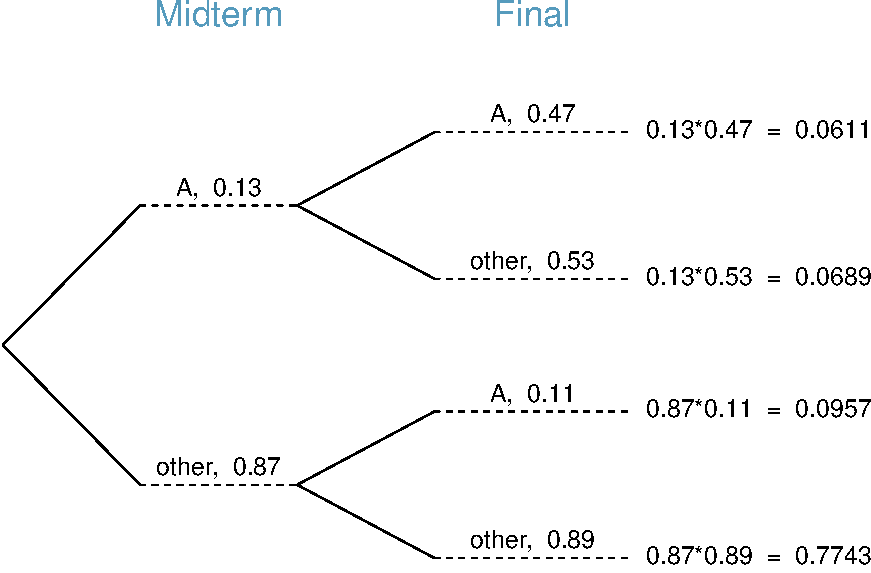
\includegraphics{_main_files/figure-latex/testTree-1.pdf}
\caption{\label{fig:testTree}Um diagrama de árvora descrevendo as variáveis parcial e final.}
\end{figure}

Com o diagrama de árvore construído, podemos calcular as probabilidades necessárias:

\begin{eqnarray*}
&&P(\text{parcial = A e final = A}) = 0,0611 \\
&&P(\text{final = A})  \\
&& \quad= P(\text{parcial = outra e final = A}) + P(\text{parcial = A e final = A}) \\
&& \quad= 0,0957 + 0,0611  = 0,1568
\end{eqnarray*}

A probabilidade marginal, \(P(\text{final = A})\), foi calculado somando todas as probabilidades conjuntas no lado direito da árvore que correspondem a \emph{final = A}. Podemos agora finalmente pegar a razão das duas probabilidades:

\begin{eqnarray*}
P(\text{parcial = A} | \text{final = A}) &=& \frac{P(\text{parcial = A e final = A})}{P(\text{final = A})} \\
&=& \frac{0,0611}{0,1568} = 0,3897
\end{eqnarray*}

A probabilidade de o aluno também ganhar um A no meio do ano é de cerca de 0,39.

\begin{center}\rule{0.5\linewidth}{0.5pt}\end{center}

\begin{exercise}
\protect\hypertarget{exr:unnamed-chunk-66}{}{\label{exr:unnamed-chunk-66} }Após um curso de estatística introdutória, 78\% dos alunos podem construir com sucesso diagramas de árvore. Daqueles que podem construir diagramas de árvores, 97\% foram aprovados, enquanto apenas 57\% dos alunos que não puderam construir diagramas de árvores foram aprovados.\footnote{(a) O diagrama da árvore é mostrado à direita. (b) Identificar quais duas probabilidades conjuntas representam os alunos que passaram e adicioná-los: \(P(\text{passou}) = 0,7566+0,1254= 0,8820\). (c) \(P(\text{diagrama de árvore de construção | passou}) = \frac{0.7566}{0.8820} = 0.8578\).}
(a) Organize esta informação em um diagrama de árvore.
(b) Qual é a probabilidade de um aluno selecionado aleatoriamente passar?
(c)Computar a probabilidade de um aluno ser capaz de construir um diagrama de árvore, se é sabido que ele passou.
\end{exercise}

\begin{center}\rule{0.5\linewidth}{0.5pt}\end{center}

\hypertarget{bayesTheoremSubsection}{%
\subsection{Teorema de Bayes}\label{bayesTheoremSubsection}}

Em muitos casos, nos é dada uma probabilidade condicional da forma

\begin{align*}
P(\text{ declaração sobre a variável 1} | \text{ declaração sobre a variável 2})
\end{align*}

mas nós realmente gostaríamos de saber a probabilidade condicional invertida:

\begin{align*}
P(\text{ declaração sobre a variável 2} | \text{ declaração sobre a variável 1})
\end{align*}

Diagramas de árvore podem ser usados para encontrar a segunda probabilidade condicional quando dada a primeira. No entanto, às vezes, não é possível desenhar o cenário em um diagrama de árvore. Nestes casos, podemos aplicar uma fórmula muito útil e geral: o Teorema de Bayes.

Primeiramente, examinamos criticamente um exemplo de inversão de probabilidades condicionais em que ainda aplicamos um diagrama de árvore.

\begin{example}
\protect\hypertarget{exm:probabilityOfBreastCancerGivenPositiveTestExample}{}{\label{exm:probabilityOfBreastCancerGivenPositiveTestExample} }No Canadá, cerca de 0,35\% de mulheres com mais de 40 anos desenvolverão câncer de mama em qualquer ano. Um teste de rastreamento comum para o câncer é a mamografia, mas esse teste não é perfeito. Em cerca de 11\% dos pacientes com câncer de mama, o teste dá um \emph{falso negativo}: indica que uma mulher não tem câncer de mama quando ela tem câncer de mama. Da mesma forma, o teste dá um \emph{falso positivo} em 7\% dos pacientes que não têm câncer de mama: indica que esses pacientes têm câncer de mama quando eles realmente não têm.\footnote{As probabilidades relatadas aqui foram obtidas usando estudos relatados a www.breastcancer.org e www.ncbi.nlm.nih.gov/pmc/articles/PMC1173421.} Se nós testamos uma mulher aleatória acima de 40 anos para câncer de mama usando uma mamografia e o teste voltou positivo -- ou seja, o teste sugeriu que o paciente tem câncer -- qual é a probabilidade de o paciente realmente ter câncer de mama?
\end{example}

\begin{figure}
\centering
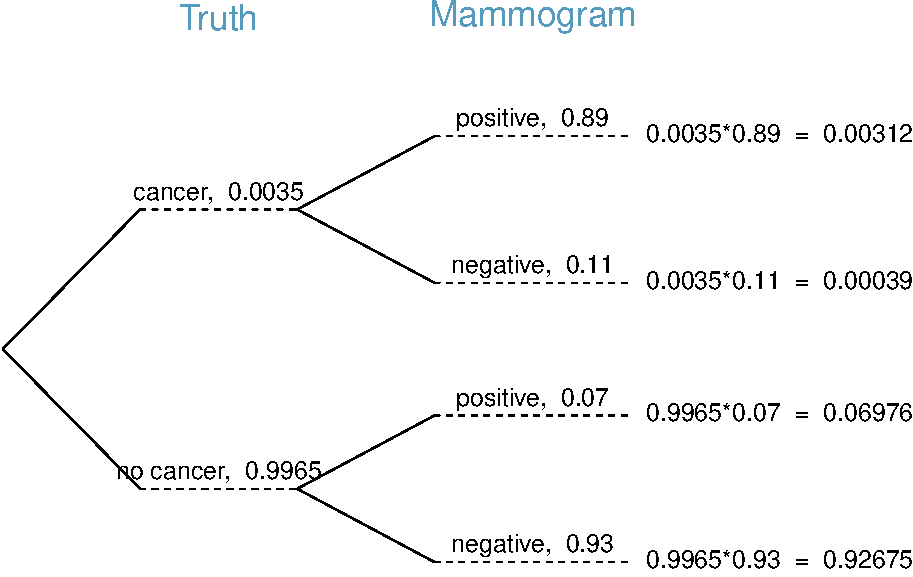
\includegraphics{_main_files/figure-latex/BreastCancerTreeDiagram-1.pdf}
\caption{\label{fig:BreastCancerTreeDiagram}Diagrama de árvore para o Exemplo acima, calculando a probabilidade de um paciente aleatório que testa positivo em uma mamografia realmente ter câncer de mama.}
\end{figure}

Observe que nos é dada informação suficiente para calcular rapidamente a probabilidade de testes positivos se uma mulher tiver câncer de mama (\$ 1.00-0.11 = 0.89 \$). No entanto, buscamos a probabilidade invertida: de câncer, dado um resultado positivo. (Cuidado com a linguagem médica não intuitiva: um resultado positivo\}do teste sugere a possível presença de câncer em um rastreamento mamográfico.) Esta probabilidade invertida pode ser dividida em dois pedaços:

\begin{align*}
P(\text{tem CM  |  mamografia}^+) = \frac{P(\text{ tem CM e mamografia}^+)}{P(\text{ mamografia}^+)}
\end{align*}

onde \emph{tem CM} é uma abreviação para o paciente realmente ter câncer de mama e mamografia\(^+\) significa que o rastreio da mamografia foi positivo. Um diagrama em árvore é útil para identificar cada probabilidade e é mostrado na Figura \ref{fig:BreastCancerTreeDiagram}. A probabilidade de o paciente ter câncer de mama e a mamografia ser positiva é

\begin{align*}
P(\text{ tem CM e mamografia}^+) &= P(\text{ mamografia}^+ | \text{ tem CM})P(\text{tem CM}) \\
    &= 0,89\times 0,0035 = 0,00312
\end{align*}

A probabilidade de um resultado de teste positivo é a soma dos dois cenários correspondentes:

\begin{align*}
P(\text{mamografia}^+) &= P(\text{mamografia}^+ \text{e tem CM}) + P(\text{mamografia}^+ \text{e sem CM}) \\
    &= P(\text{tem CM})P(\text{mamografia}^+ | \text{ tem CM}) \\
    &\qquad\qquad   + P(\text{sem CM})P(\text{mamografia}^+ | \text{ sem CM}) \\
    &= 0,0035\times 0,89 + 0,9965\times 0,07 = 0,07288
\end{align*}

Então, se a triagem mamográfica for positiva para um paciente, a probabilidade de o paciente ter câncer de mama é

\begin{align*}
P(\text{tem CM } | \text{ mamografia}^+)
    &= \frac{P(\text{tem CM e mamografia} ^+)}{P(\text{mamografia}^+)}\\
    &= \frac{0.00312}{0.07288} \approx 0.0428
\end{align*}

Ou seja, mesmo que um paciente tenha uma triagem mamográfica positiva, ainda há apenas uma chance de 4\% que ela tenha câncer de mama.

O Exemplo \ref{exm:probabilityOfBreastCancerGivenPositiveTestExample} destaca por que os médicos geralmente realizam mais testes, independentemente do primeiro resultado positivo do teste. Quando uma condição médica é rara, um único teste positivo geralmente não é definitivo.

Considere novamente a última equação do Exemplo \ref{exm:probabilityOfBreastCancerGivenPositiveTestExample}.
Usando o diagrama de árvore, podemos ver que o numerador (o topo da fração) é igual ao seguinte produto:

\begin{align*}
P(\text{tem CM e mamografia}^+) = P(\text{mamografia}^+ | \text{ tem CM})P(\text{tem CM})
\end{align*}

O denominador -- a probabilidade de o rastreamento ser positivo -- é igual à soma das probabilidades para cada cenário de rastreamento positivo:

\begin{align*}
P(\text{mamografia}^+)
    &= P(\text{mamografia}^+\text{ e sem CM})
        + P(\text{mamografia}^+\text{ e tem CM})
\end{align*}

No exemplo, cada uma das probabilidades no lado direito foi dividida em um produto de uma probabilidade condicional e probabilidade marginal usando o diagrama de árvore.

\begin{align*}
P(\text{mamografia}^+)
&= P(\text{mamografia}^+\text{ e sem CM}) + P(\text{mamografia}^+\text{ e tem CM}) \\
&= P(\text{mamografia}^+ | \text{ sem CM})P(\text{sem CM}) + P(\text{mamografia}^+ | \text{ tem CM})P(\text{tem CM})
\end{align*}

Podemos ver uma aplicação do Teorema de Bayes substituindo as expressões de probabilidade resultantes no numerador e no denominador da probabilidade condicional original.

\begin{align*}
& P(\text{tem CM } | \text{ mamografia}^+)
= \frac{P(\text{mamografia}^+ | \text{ tem CM})P(\text{tem CM})}
    {P(\text{mamografia}^+ | \text{ sem CM})P(\text{sem CM}) + P(\text{mamografia}^+ | \text{ tem CM})P(\text{tem CM})}
\end{align*}

Teorema de Bayes: invertendo probabilidades: Considere a seguinte probabilidade condicional para a variável 1 e a variável 2:

\begin{align*}
P(\text{ resultado }A_1\text{ da variável 1} | \text{ resultado B da variável 2})
\end{align*}

O Teorema de Bayes afirma que essa probabilidade condicional pode ser identificada como a seguinte fração:

\begin{align}
\frac{P(B | A_1) P(A_1)}
    {P(B | A_1) P(A_1) + P(B | A_2) P(A_2) + \cdots + P(B | A_k) P(A_k)}
    \label{eq:equationOfBayesTheorem}
\end{align}

onde \(A_2, A_3, \dots, A_k\) representam todos os outros resultados possíveis da primeira variável.

O Teorema de Bayes é apenas uma generalização do que fizemos usando diagramas de árvores. O numerador identifica a probabilidade de obter \(A_1\) e \(B\). O denominador é a probabilidade marginal de obter \(B\). Este componente inferior da fração parece longo e complicado, uma vez que temos que somar probabilidades de todas as maneiras diferentes para obter \(B\). Nós sempre completamos este passo quando usamos diagramas de árvores. No entanto, nós geralmente fizemos isso em uma etapa separada para que não parecesse tão complexo.

Para aplicar o Teorema de Bayes corretamente, existem duas etapas preparatórias:

\begin{itemize}
\item
  Primeiro, identifique as probabilidades marginais de cada resultado possível da primeira variável: \(P(A_1), P(A_2), \dots, P(A_k)\).
\item
  Em seguida, identifique a probabilidade do resultado \(B\), condicionada em cada cenário possível para a primeira variável: \(P(B | A_1), P(B | A_2), \dots, P(B | A_k)\).
\end{itemize}

Uma vez que cada uma dessas probabilidades sejam identificadas, elas podem ser aplicadas diretamente dentro da fórmula.

Dica: Use somente o Teorema de Bayes quando os diagramas de árvore são difíceis: Desenhar um diagrama de árvore facilita a compreensão de como duas variáveis estão conectadas. Use o Teorema de Bayes somente quando houver muitos cenários que desenhar um diagrama de árvore seria complexo.

\begin{center}\rule{0.5\linewidth}{0.5pt}\end{center}

\begin{exercise}
\protect\hypertarget{exr:exerciseForParkingLotOnCampusBeingFullAndWhetherOrNotThereIsASportingEvent}{}{\label{exr:exerciseForParkingLotOnCampusBeingFullAndWhetherOrNotThereIsASportingEvent} }José visita o campus toda quinta-feira à noite. No entanto, alguns dias a garagem está cheia, muitas vezes devido a eventos universitários. Há eventos acadêmicos em 35\% das noites, eventos esportivos em 20\% das noites e nenhum evento em 45\% das noites. Quando há um evento acadêmico, a garagem está cheia em 25\% do tempo, e 70\% em noites com eventos esportivos. Nas noites em que não há eventos, ela está cheia somente em 5\% do tempo. Se José vem ao campus e encontra a garagem cheia, qual é a probabilidade de haver um evento esportivo? Use um diagrama de árvore para resolver este problema.\footnote{O diagrama da árvore, com três ramificações principais, fica a critério do aluno desenhar. Em seguida, identificamos duas probabilidades no diagrama em árvore. (1) A probabilidade de que haja um evento esportivo e a garagem esteja cheia: 0.14. (2) A probabilidade de a garagem estar cheia: \(0,0875 + 0,14 + 0,0225 = 0,25\). Então a solução é a razão dessas probabilidades: \(\frac{0,14}{0,25} = 0,56\). Se a garagem estiver cheia, existe uma probabilidade de 56\% de haver um evento esportivo.}
\end{exercise}

\begin{center}\rule{0.5\linewidth}{0.5pt}\end{center}

\begin{example}
\protect\hypertarget{exm:unnamed-chunk-67}{}{\label{exm:unnamed-chunk-67} }Aqui nós resolvemos o mesmo problema apresentado na Prática Orientada \ref{exr:exerciseForParkingLotOnCampusBeingFullAndWhetherOrNotThereIsASportingEvent}, exceto que desta vez usamos o Teorema de Bayes.
\end{example}

O resultado do interesse é saber se há um evento esportivo (ligue para esse valor de \(A_1\)) e a condição é que o lote esteja cheio (\(B\)). Deixe \(A_2\) representar um evento acadêmico e \(A_3\) representam não haver evento no campus. Então as probabilidades dadas podem ser escritas como

\begin{align*}
&P(A_1) = 0,2 &&P(A_2) = 0,35 &&P(A_3) = 0,45 \\
&P(B | A_1) = 0,7 &&P(B | A_2) = 0,25 &&P(B | A_3) = 0,05
\end{align*}

Teorema de Bayes pode ser usado para calcular a probabilidade de um evento esportivo (\(A_1\)) sob a condição de que o estacionamento esteja cheio (\(B\)):

\begin{align*}
P(A_1 | B) &= \frac{P(B | A_1) P(A_1)}{P(B | A_1) P(A_1) + P(B | A_2) P(A_2) + P(B | A_3) P(A_3)} \\
        &= \frac{(0,7)(0,2)}{(0,7)(0,2) + (0,25)(0,35) + (0,05)(0,45)} \\
        &= 0.56 
\end{align*}

Com base nas informações de que a garagem está cheia, há uma probabilidade de 56\% de que um evento esportivo seja realizado no campus naquela noite.

\begin{center}\rule{0.5\linewidth}{0.5pt}\end{center}

\begin{exercise}
\protect\hypertarget{exr:exerciseForParkingLotOnCampusBeingFullAndWhetherOrNotThereIsAnAcademicEvent}{}{\label{exr:exerciseForParkingLotOnCampusBeingFullAndWhetherOrNotThereIsAnAcademicEvent} }Use as informações do exercício anterior e o exemplo para verificar se a probabilidade de que haja um evento acadêmico condicionado ao estacionamento estar cheio é de 0,35.\footnote{Resposta curta: \(P(A_2 | B) = \frac{P(B | A_2) P(A_2)}{P(B | A_1) P(A_1) + P(B | A_2) P(A_2) + P(B | A_3) P(A_3)} = \frac{(0,25)(0,35)}{(0,7)(0,2) + (0,25)(0,35) + (0,05)(0,45)} = 0,35\)}
\end{exercise}

\begin{center}\rule{0.5\linewidth}{0.5pt}\end{center}

\begin{center}\rule{0.5\linewidth}{0.5pt}\end{center}

\begin{exercise}
\protect\hypertarget{exr:exerciseForParkingLotOnCampusBeingFullAndWhetherOrNotThereIsNoEvent}{}{\label{exr:exerciseForParkingLotOnCampusBeingFullAndWhetherOrNotThereIsNoEvent} }Na Prática Orientada \ref{exr:exerciseForParkingLotOnCampusBeingFullAndWhetherOrNotThereIsASportingEvent} e \ref{exr:exerciseForParkingLotOnCampusBeingFullAndWhetherOrNotThereIsAnAcademicEvent}, você descobriu que, se o estacionamento está cheio, a probabilidade de haver um evento esportivo é de 0.56 e a probabilidade de haver um evento acadêmico é de 0.35. Usando esta informação, calcule \(P( \text{sem evento | a garagem está cheia})\).\footnote{Cada probabilidade é condicionada à mesma informação que a garagem está cheia, então o complemento pode ser usado: \(1.00 - 0.56 - 0,35 = 0,09\).}
\end{exercise}

\begin{center}\rule{0.5\linewidth}{0.5pt}\end{center}

Os últimos exercícios ofereceram uma maneira de atualizar nossa crença sobre se há um evento esportivo, um evento acadêmico ou nenhum evento acontecendo na escola com base nas informações de que o estacionamento estava lotado. Essa estratégia de \emph{atualizar crenças} usando o Teorema de Bayes é, na verdade, a base de toda uma seção de estatísticas chamada de \textbf{Estatística Bayesiana}. Embora as estatísticas bayesianas sejam muito importantes e úteis, não teremos tempo para abordar muito mais delas neste livro.

\hypertarget{smallPop}{%
\section{Amostragem de uma população pequena (tópico especial)}\label{smallPop}}

\begin{example}
\protect\hypertarget{exm:unnamed-chunk-68}{}{\label{exm:unnamed-chunk-68} }Os professores às vezes escolhem um aluno aleatoriamente para responder a uma pergunta. Se cada aluno tiver uma chance igual de ser selecionado e houver 15 pessoas na sua turma, qual é a chance de ela escolher você para a próxima pergunta?
\end{example}

Se há 15 pessoas para perguntar, então a probabilidade é \(1/15\), ou \(0.067\).

\begin{example}
\protect\hypertarget{exm:3woRep}{}{\label{exm:3woRep} }Se o professor fizer 3 perguntas, qual é a probabilidade de você não ser selecionado? Suponha que ele não vai escolher a mesma pessoa duas vezes em uma determinada palestra.
\end{example}

Para a primeira pergunta, ele escolherá outra pessoa com probabilidade de \(14/15\). Quando ele faz a segunda pergunta, ela só tem 14 pessoas que ainda não foram perguntadas. Assim, se você não foi escolhido na primeira pergunta, a probabilidade de você não ser novamente escolhido é \(13/14\). Da mesma forma, a probabilidade de você não ser novamente escolhido na terceira pergunta é de \(12/13\), e a probabilidade de não ser escolhido para qualquer uma das três perguntas é

\begin{eqnarray*}
&&P(\text{não chamar em 3 perguntas})
\\
&&\quad= P(\text{Q1} = \text{não escolhido}, \text{Q2} = \text{não escolhido}, \text{Q3} = \text{não escolhido}) \\
&&\quad = \frac{14}{15}\times\frac{13}{14}\times\frac{12}{13} = \frac{12}{15} = 0.80
\end{eqnarray*}

\begin{center}\rule{0.5\linewidth}{0.5pt}\end{center}

\begin{exercise}
\protect\hypertarget{exr:unnamed-chunk-69}{}{\label{exr:unnamed-chunk-69} }Qual regra nos permitiu multiplicar as probabilidades no Exemplo \ref{exm:3woRep}?\footnote{As três probabilidades que calculamos eram na verdade uma probabilidade marginal, \(P(Q1 = \text{não escolhido})\) e duas probabilidades condicionais: \(P(\text{Q2 = não escolhido} |\text{Q1} = \text{não escolhido}) \text{ e } P(\text{Q3} = \text{não escolhido} |\text{ Q1} = \text{não escolhido}, \text{Q2} = \text{não escolhido})\). Usando a Regra Geral de Multiplicação, o produto dessas três probabilidades é a probabilidade de não ser escolhido em 3 questões.}
\end{exercise}

\begin{center}\rule{0.5\linewidth}{0.5pt}\end{center}

\begin{example}
\protect\hypertarget{exm:3wRep}{}{\label{exm:3wRep} }Suponha que o professor escolha aleatoriamente sem considerar quem ele já selecionou, ou seja, os alunos podem ser escolhidos mais de uma vez. Qual é a probabilidade de você não ser escolhido para nenhuma das três perguntas?
\end{example}

Cada escolha é independente e a probabilidade de não ser escolhido para qualquer questão individual é de \(14/15\). Assim, podemos usar a regra de multiplicação para processos independentes.

\begin{eqnarray*}
&&P(\text{ não pegou em 3 perguntas}) \\
&&\quad = P(\text{Q1} = \text{não escolhido}, \text{Q2} = \text{não escolhido}, \text{Q3} = \text{não escolhido}.) \\
&&\quad = \frac{14}{15}\times\frac{14}{15}\times\frac{14}{15} = 0,813
\end{eqnarray*}

Você tem uma chance um pouco maior de não ser escolhida em comparação a quando ela escolheu uma nova pessoa para cada pergunta. No entanto, você agora pode ser escolhido mais de uma vez.

\begin{center}\rule{0.5\linewidth}{0.5pt}\end{center}

\begin{exercise}
\protect\hypertarget{exr:unnamed-chunk-70}{}{\label{exr:unnamed-chunk-70} }Sob a configuração do Exemplo \ref{exm:3wRep}, qual é a probabilidade de ser escolhido para responder a todas as três perguntas?\footnote{\(P(\text{sendo escolhido para responder a todas as três perguntas}) = \left(\frac{1}{15}\right)^3 = 0,00030\).}
\end{exercise}

\begin{center}\rule{0.5\linewidth}{0.5pt}\end{center}

Se nós provamos de uma pequena população \textbf{sem reposição}, nós não temos mais independência entre nossas observações. No Exemplo \ref{exm:3woRep}, a probabilidade de não ser escolhido para a segunda questão estava condicionada ao fato de você não ter sido escolhido para a primeira questão. No Exemplo \ref{exm:3wRep}, a professora escolheu seus alunos \emph{com substituição}: ela repetidamente escolheu entre a turma inteira sem considerar quem ela já havia escolhido.

\begin{center}\rule{0.5\linewidth}{0.5pt}\end{center}

\begin{exercise}
\protect\hypertarget{exr:raffleOf30TicketsWWOReplacement}{}{\label{exr:raffleOf30TicketsWWOReplacement} }Seu departamento está sorteando uma rifa. Eles vendem 30 ingressos e oferecem sete prêmios.
(a) Colocam os ingressos em um chapéu e pegam um para cada prêmio. Os bilhetes são amostrados sem substituição, ou seja, os bilhetes selecionados não são colocados de volta no chapéu. Qual é a probabilidade de ganhar um prêmio se você comprar um ingresso?
(b) E se os bilhetes forem amostrados com substituição?\footnote{(a) Primeiro determine a probabilidade de não ganhar. Os bilhetes são amostrados sem substituição, o que significa que a probabilidade de você não ganhar no primeiro sorteio é \(29/30\), \(28/29\) para o segundo, \ldots, e \(23/24\) para o sétimo. A probabilidade de você não ganhar nenhum prêmio é o produto dessas probabilidades separadas: \(23/30\). Ou seja, a probabilidade de ganhar um prêmio é \(1 - 23/30 = 7/30 = 0,233\). (b) Quando os bilhetes são amostrados com reposição, há sete sorteios independentes. Novamente, primeiro encontramos a probabilidade de não ganhar um prêmio: \((29/30)^7 = 0,789\). Assim, a probabilidade de ganhar (pelo menos) um prêmio ao sortear com reposição é 0,211.}
\end{exercise}

\begin{center}\rule{0.5\linewidth}{0.5pt}\end{center}

\begin{center}\rule{0.5\linewidth}{0.5pt}\end{center}

\begin{exercise}
\protect\hypertarget{exr:followUpToRaffleOf30TicketsWWOReplacement}{}{\label{exr:followUpToRaffleOf30TicketsWWOReplacement} }Compare suas respostas na Prática Orientada \ref{exr:raffleOf30TicketsWWOReplacement}. Quanta influência o método de amostragem tem sobre suas chances de ganhar um prêmio?\footnote{Existe uma chance 10\% maior de ganhar um prêmio ao usar amostragem sem reposição. No entanto, no máximo um prêmio pode ser ganho sob este procedimento de amostragem.}
\end{exercise}

\begin{center}\rule{0.5\linewidth}{0.5pt}\end{center}

Se tivéssemos repetido a Prática Orientada \ref{exr:raffleOf30TicketsWWOReplacement} com 300 tíquetes em vez de 30, teríamos encontrado algo interessante: os resultados seriam quase idênticos. A probabilidade seria 0,0233 sem reposição e 0,0231 com reposição. Quando o tamanho da amostra é apenas uma pequena fração da população (abaixo de 10\%), as observações são quase independentes, mesmo quando a amostragem é feita sem reposição.

\hypertarget{randomVariablesSection}{%
\section{Variáveis aleatórias (tópico especial)}\label{randomVariablesSection}}

\begin{example}
\protect\hypertarget{exm:bookStoreSales}{}{\label{exm:bookStoreSales} }Dois livros são atribuídos para uma aula de estatística: um livro didático e seu guia de estudo correspondente. A livraria da universidade determinou que 20\% dos estudantes matriculados não compram nenhum dos livros, 55\% apenas compram um livro e 25\% compram ambos os livros, e essas porcentagens são relativamente constantes de um semestre para outro. Se houver 100 alunos inscritos, quantos livros a livraria espera vender para essa classe?
\end{example}

Cerca de 20 alunos não compram nenhum livro (0 livros no total), cerca de 55 compram um livro (55 livros no total) e cerca de 25 compram dois livros (totalizando 50 livros para estes 25 alunos). A livraria deve vender cerca de 105 livros para esta classe.

\begin{center}\rule{0.5\linewidth}{0.5pt}\end{center}

\begin{exercise}
\protect\hypertarget{exr:unnamed-chunk-71}{}{\label{exr:unnamed-chunk-71} }Você ficaria surpreso se a livraria vendesse um pouco mais de 105 livros?\footnote{Se eles vendem um pouco mais ou um pouco menos, isso não deve ser uma surpresa. Esperançosamente o Capítulo de Introdução ajudou a deixar claro que há variabilidade natural nos dados observados. Por exemplo, se jogássemos uma moeda 100 vezes, ela normalmente não virá cara metade do tempo, mas provavelmente será perto.}
\end{exercise}

\begin{center}\rule{0.5\linewidth}{0.5pt}\end{center}

\begin{example}
\protect\hypertarget{exm:bookStoreRev}{}{\label{exm:bookStoreRev} }O livro custa \$137 e o guia de estudo \$33. Quanta receita a livraria deve esperar desta turma de 100 alunos?
\end{example}

Cerca de 55 alunos irão apenas comprar um livro didático, fornecendo receita de

\begin{eqnarray*}
\$137 \times  55 = \$7.535
\end{eqnarray*}

Cerca de 25 alunos que compram o livro didático e o guia de estudo pagariam um total de

\begin{eqnarray*}
(\$137 + \$33) \times  25 = \$170 \times  25 = \$4,250
\end{eqnarray*}

Assim, a livraria deve gerar cerca de \(\$7.535 + \$4.250 = \$11.785\) desses 100 alunos para essa classe. No entanto, pode haver alguma \textbf{variabilidade de amostragem} para que a quantidade real possa diferir um pouco.

\begin{figure}
\centering
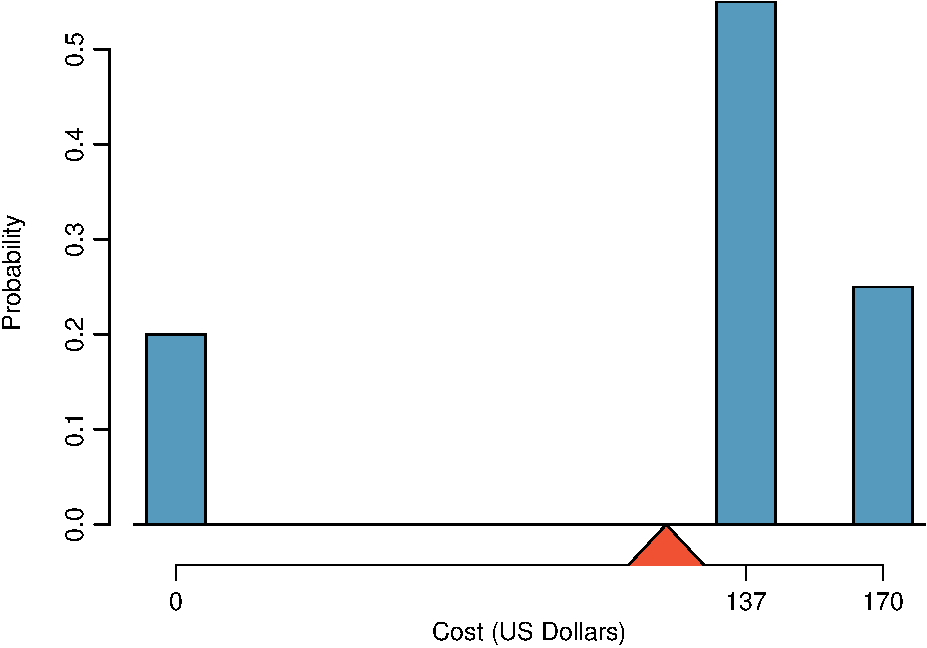
\includegraphics{_main_files/figure-latex/bookCostDist-1.pdf}
\caption{\label{fig:bookCostDist}Distribuição de probabilidade para a receita da livraria de um único aluno. A distribuição se equilibra em um triângulo representando a receita média por estudante.}
\end{figure}

\begin{example}
\protect\hypertarget{exm:revFromStudent}{}{\label{exm:revFromStudent} }Qual é a receita média por aluno para este curso?
\end{example}

A receita total esperada é de \$11.785 e há 100 alunos. Portanto, a receita esperada por aluno é \(\$11,785/100 = \$117.85\).

\hypertarget{expectation}{%
\subsection{Experança}\label{expectation}}

Chamamos uma variável ou processo com um resultado numérico de \textbf{variável aleatória}, e geralmente representamos essa variável aleatória com uma letra maiúscula, como \(X\), \(Y\) ou \(Z\). A quantidade de dinheiro que um único aluno gastará em seus livros de estatística é uma variável aleatória, e nós a representamos por \(X\).

Variável aleatória: Um processo aleatório ou variável com um resultado numérico.

Os possíveis resultados de \(X\) são rotulados com uma letra minúscula correspondente \(x\) e subscritos. Por exemplo, nós escrevemos \(x_1=\$0\), \(x_2=\$137\), e \(x_3=\$170\), que ocorrem com probabilidades de \(0,20\), \(0,55\) e \(0,25\). A distribuição de \(X\) é resumida na Figura \ref{fig:bookCostDist} e Tabela \ref{tab:statSpendDist}.

\begin{table}

\caption{\label{tab:statSpendDist}A distribuição de probabilidade para a variável aleatória X, representando a receita da livraria de um único aluno.}
\centering
\begin{tabular}[t]{l|c|c|c|c}
\hline
  & 1 & 2 & 3 & Total\\
\hline
i & \$0 & \$137 & \$170 & -\\
\hline
P(X = xi) & 0.2 & 0.55 & 0.25 & 1\\
\hline
\end{tabular}
\end{table}

Calculamos o resultado médio de \(X\) como \$117,85 no Exemplo \ref{exm:revFromStudent}. Chamamos essa média de \textbf{valor esperado} de \(X\), denotado por \(E(X)\). O valor esperado de uma variável aleatória é calculado adicionando cada resultado ponderado por sua probabilidade:

\begin{align*}
E(X) &= 0 \times  P(X=0) + 137 \times  P(X=137) + 170 \times  P(X=170) \\
    &= 0 \times  0.20 + 137 \times  0.55 + 170 \times  0.25 = 117.85
\end{align*}

Valor esperado de uma variável aleatória discreta: Se \(X\) tiver resultados \(x_1, \dots, x_k\) com probabilidades \(P(X=x_1),\dots, P(X=x_k)\), o valor esperado de \(X\) é a soma de cada resultado multiplicado por sua probabilidade correspondente:

\begin{align}
E(X)    &= x_1\times P(X=x_1) + \cdots + x_k\times P(X=x_k) \notag \\
    &= \sum_{i=1}^{k}x_iP(X=x_i)
\end{align}

A letra grega \(\mu\) pode ser usado no lugar da notação \(E(X)\).

O valor esperado de uma variável aleatória representa o resultado médio. Por exemplo, \(E(X) = 117,85\) representa o valor médio que a livraria espera fazer de um único aluno, que também poderíamos escrever como \(\mu=117.85\).

Também é possível calcular o valor esperado de uma variável aleatória contínua (veja a Seção \ref{contDist}. No entanto, requer um pouco de cálculo e nós o salvamos para uma aula posterior.\footnote{\(\mu = \int xf(x)dx\) onde \(f(x)\) representa uma função para a curva de densidade.}

Na física, a esperança tem o mesmo significado que o centro de gravidade. A distribuição pode ser representada por uma série de pesos em cada resultado e a média representa o ponto de equilíbrio. Isso é representado nas Figuras \ref{fig:bookCostDist} e \ref{fig:bookWts}. A ideia de um centro de gravidade também se expande para distribuições de probabilidade contínuas. Figura \ref{fig:contBalance} mostra uma distribuição de probabilidade contínua equilibrada sobre uma cunha colocada na média.

\begin{figure}
\centering
\includegraphics{_main_files/figure-latex/bookWts-1.pdf}
\caption{\label{fig:bookWts}Um sistema de pesos representando a distribuição de probabilidade para \(X\). A corda mantém a distribuição na média para manter o sistema balanceado.}
\end{figure}

\begin{figure}
\centering
\includegraphics{_main_files/figure-latex/contBalance-1.pdf}
\caption{\label{fig:contBalance}Uma distribuição contínua também pode ser balanceada em sua média.}
\end{figure}

\hypertarget{variabilityRandomVariables}{%
\subsection{Variabilidade em variáveis aleatórias}\label{variabilityRandomVariables}}

Suponha que você administrasse a livraria da universidade. Além de quanto receita você espera gerar, você também pode querer saber a volatilidade (variabilidade) de sua receita.

A \textbf{variância} e \textbf{desvio padrão} pode ser usado para descrever a variabilidade de uma variável aleatória. A Seção \ref{variability} introduziu um método para encontrar a variância e desvio padrão para um conjunto de dados. Nós primeiro calculamos desvios da média (\(x_i - \mu\)), eleva ao quadrado esses desvios, e faz uma média para obter a variância. No caso de uma variável aleatória, novamente calculamos os desvios quadrados. No entanto, consideramos a soma ponderada pelas probabilidades correspondentes, exatamente como fizemos para a esperança. Essa soma ponderada de desvios quadrados é igual à variância e calculamos o desvio padrão tomando a raiz quadrada da variância, como fizemos na Seção \ref{variability}.

Fórmula geral da variância: Se \(X\) leva os resultados \(x_1, \dots, x_k\) com probabilidades \(P(X=x_1), \dots, P(X=x_k)\) e valor esperado \(\mu=E(X)\), então a variância de \(X\), denotada por \(Var(X)\) ou o símbolo \(\sigma^2\), é

\begin{align}
\sigma^2 &= (x_1-\mu)^2\times P(X=x_1) + \cdots \notag \\
    & \qquad\quad\cdots+ (x_k-\mu)^2\times P(X=x_k) \notag \\
    &= \sum_{j=1}^{k} (x_j - \mu)^2 P(X=x_j)
\end{align}

O desvio padrão de \(X\), rotulado \(\sigma\), é a raiz quadrada da variância.

\begin{example}
\protect\hypertarget{exm:unnamed-chunk-72}{}{\label{exm:unnamed-chunk-72} }Calcule o valor esperado, a variação e o desvio padrão de \(X\), a receita de um único estudante de estatística para a livraria.
\end{example}

É útil construir uma tabela que armazene os cálculos para cada resultado separadamente e depois some os resultados.

\begin{tabular}{l|c|c|c|c}
\hline
  & 1 & 2 & 3 & Total\\
\hline
i & \$0 & \$137 & \$170 & -\\
\hline
P(X = xi) & 0.2 & 0.55 & 0.25 & 1\\
\hline
xi * P(X = xi) & 0 & 75.35 & 42.5 & 117.85\\
\hline
\end{tabular}

Assim, o valor esperado é \(\mu = 117,85\), que calculamos anteriormente. A variância pode ser construída estendendo essa tabela:

\begin{tabular}{l|c|c|c|c}
\hline
  & 1 & 2 & 3 & Total\\
\hline
i & \$0 & \$137 & \$170 & -\\
\hline
P(X = xi) & 0.2 & 0.55 & 0.25 & 1\\
\hline
xi * P(X = xi) & 0 & 75.35 & 42.5 & 117.85\\
\hline
xi - mu & -117.85 & 19.15 & 52.15 & \\
\hline
(xi - mu)² & 13888.62 & 366.72 & 2719.62 & \\
\hline
(xi - mu)² * P(X = xi) & 2777.7 & 201.7 & 679.9 & 3659.3\\
\hline
\end{tabular}

A variação de \(X\) é \(\sigma^2 = 3659,3\), o que significa que o desvio padrão é \(\sigma = \sqrt{3659,3} = \$60,49\).

\begin{center}\rule{0.5\linewidth}{0.5pt}\end{center}

\begin{exercise}
\protect\hypertarget{exr:unnamed-chunk-75}{}{\label{exr:unnamed-chunk-75} }A livraria também oferece um livro de química por \$159 e um complemento para o livro por \$41. A partir da experiência passada, eles sabem que cerca de 25\% de estudantes de química apenas compram o livro enquanto 60\% compram o livro e o suplemento.\footnote{(a) 100\% - 25\% - 60\% = 15\% dos alunos não compram livros na turma. A parte (b) é representada por \(y_i = [0.00, 159.00, 200.00]\), para 1 (nenhum livro), 2(livro didático) e 3 (ambos), respectivamente. E \$P(Y = y\_i) = 0.15, 0.25, 0.60}\$. A esperança para a parte (c) é dada como o total de \(y_i\times P(Y=y_i) = 159,75\). O resultado da parte (d) é a raiz quadrada da variância: \(\sigma = \sqrt{Var(Y)} = \$69,28\).{]}
(a) Que proporção de estudantes não compra um dos livros? Suponha que nenhum aluno compre o suplemento sem o livro didático.
(b) Se \(Y\) representar a receita de um único aluno. Escreva a distribuição de probabilidade de \(Y\), ou seja, uma tabela para cada resultado e sua probabilidade associada.
(c) Calcule a receita esperada de um único estudante de química.
(d) Encontre o desvio padrão para descrever a variabilidade associada à receita de um único aluno.
\end{exercise}

\begin{center}\rule{0.5\linewidth}{0.5pt}\end{center}

\hypertarget{linearCombinationRandomVariables}{%
\subsection{Combinações lineares de variáveis aleatórias}\label{linearCombinationRandomVariables}}

Até agora, pensamos que cada variável é uma história completa em si mesma. Às vezes é mais apropriado usar uma combinação de variáveis. Por exemplo, a quantidade de tempo que uma pessoa gasta diariamente para ir ao trabalho pode ser dividida em vários deslocamentos diários. Da mesma forma, o ganho ou a perda total em uma carteira de ações é a soma dos ganhos e perdas em seus componentes.

\begin{example}
\protect\hypertarget{exm:unnamed-chunk-76}{}{\label{exm:unnamed-chunk-76} }John viaja para o trabalho cinco dias por semana. Usaremos \(X_1\) para representar seu tempo de viagem na segunda-feira, \(X_2\) para representar seu tempo de viagem na terça-feira e assim por diante. Escreva uma equação usando \(X_1, \dots, X_5\) que representa seu tempo de viagem para a semana, denotado por \(W\).
\end{example}

Seu tempo total de viagem semanal é a soma dos cinco valores diários:
\[W = X_1 + X_2 + X_3 + X_4 + X_5\]
Quebrar o tempo de viagem semanal \(W\) em pedaços fornece uma estrutura para entender cada fonte de aleatoriedade e é útil para modelar \(W\).

\begin{example}
\protect\hypertarget{exm:unnamed-chunk-77}{}{\label{exm:unnamed-chunk-77} }John leva uma média de 18 minutos por dia para ir ao trabalho. O que você esperaria que seu tempo médio de deslocamento fosse na semana?
\end{example}

Fomos informados de que a média (ou seja, o valor esperado) do tempo de viagem é de 18 minutos por dia: \(E(X_i) = 18\). Para obter o tempo esperado para a soma dos cinco dias, podemos adicionar o tempo esperado para cada dia individual:

\begin{align*}
E(W) &= E(X_1 + X_2 + X_3 + X_4 + X_5) \\
    &= E(X_1) + E(X_2) + E(X_3) + E(X_4) + E(X_5) \\
    &= 18 + 18 + 18 + 18 + 18 = 90\text{ minutos}
\end{align*}

A esperança do tempo total é igual à soma dos tempos individuais esperados. Mais geralmente, a esperança de uma soma de variáveis aleatórias é sempre a soma da esperança para cada variável aleatória.

\begin{center}\rule{0.5\linewidth}{0.5pt}\end{center}

\begin{exercise}
\protect\hypertarget{exr:elenaIsSellingATVAndBuyingAToasterOvenAtAnAuction}{}{\label{exr:elenaIsSellingATVAndBuyingAToasterOvenAtAnAuction} }Elena está vendendo uma TV em um leilão a dinheiro e também pretende comprar uma torradeira no leilão. Se \(X\) representa o lucro para vender a TV e \(Y\) representa o custo da torradeira, escreva uma equação que represente a mudança líquida no dinheiro de Elena.\footnote{Ela fará \(X\) dólares na TV mas gastará \(Y\) dólares na torradeira: \(X-Y\).}
\end{exercise}

\begin{center}\rule{0.5\linewidth}{0.5pt}\end{center}

\begin{center}\rule{0.5\linewidth}{0.5pt}\end{center}

\begin{exercise}
\protect\hypertarget{exr:unnamed-chunk-78}{}{\label{exr:unnamed-chunk-78} }Baseado em leilões anteriores, Elena acha que deve receber cerca de \$175 na TV e pagar cerca de \$23 pela torradeira. No total, quanto ela deve esperar receber ou gastar?\footnote{\(E(X-Y) = E(X) - E(Y) = 175 - 23 = \$152\). Ela deve esperar receber \$152.}
\end{exercise}

\begin{center}\rule{0.5\linewidth}{0.5pt}\end{center}

\begin{center}\rule{0.5\linewidth}{0.5pt}\end{center}

\begin{exercise}
\protect\hypertarget{exr:explainWhyThereIsUncertaintyInTheSum}{}{\label{exr:explainWhyThereIsUncertaintyInTheSum} }Você ficaria surpreso se o trajeto semanal de John não fosse exatamente de 90 minutos ou se Elena não fizesse exatamente \$152? Explique.\^{}´{[}Não, já que provavelmente há alguma variabilidade. Por exemplo, o tráfego varia de um dia para o outro, e os preços de leilão variam dependendo da qualidade da mercadoria e do interesse dos participantes.{]}
\end{exercise}

\begin{center}\rule{0.5\linewidth}{0.5pt}\end{center}

Dois conceitos importantes sobre combinações de variáveis aleatórias foram introduzidos até agora. Primeiro, um valor final pode às vezes ser descrito como a soma de suas partes em uma equação. Segundo, a intuição sugere que colocar os valores médios individuais nessa equação fornece o valor médio que esperamos no total. Este segundo ponto precisa de esclarecimento -- é garantido que é verdade naquilo que é chamado de \emph{combinações lineares de variáveis aleatórias}.

Uma \textbf{combinação linear} de duas variáveis aleatórias \(X\) e \(Y\) é uma frase chique para descrever uma combinação

\[ aX + bY\]

onde \(a\) e \(b\) são números fixos e conhecidos. Para o tempo de deslocamento de John, havia cinco variáveis aleatórias -- uma para cada dia de trabalho -- e cada variável aleatória poderia ser escrita como tendo um coeficiente fixo em 1:

\[1X_1 + 1 X_2 + 1 X_3 + 1 X_4 + 1 X_5\]

Para o ganho ou perda líquida de Elena, a variável aleatória \(X\) tinha um coeficiente de +1 e a variável aleatória \(Y\) tinha um coeficiente -1.

Ao considerar a média de uma combinação linear de variáveis aleatórias, é seguro inserir a média de cada variável aleatória e depois calcular o resultado final. Para alguns exemplos de combinações não-lineares de variáveis aleatórias -- casos em que não podemos simplesmente conectar os meios -- veja a nota de rodapé.\footnote{Se \(X\) e \(Y\) forem variáveis aleatórias, considere as seguintes combinações: \(X^{1+Y}\), \(X\times Y\), \(X/Y\). Nesses casos, conectar o valor médio de cada variável aleatória e calcular o resultado geralmente não resultará em um valor médio preciso para o resultado final.}

Combinações lineares de variáveis aleatórias e o resultado médio: Se \(X\) e \(Y\) são variáveis aleatórias, então uma combinação linear das variáveis aleatórias é dada por

\begin{align}
aX + bY
\label{eq:linComboOfRandomVariablesXAndY}
\end{align}

onde \(a\) e \(b\) são alguns números fixos. Para calcular o valor médio de uma combinação linear de variáveis aleatórias, conecte a média de cada variável aleatória individual e calcule o resultado:

\begin{align*}
a\times E(X) + b\times E(Y)
\end{align*}

Lembre-se de que o valor esperado é o mesmo que a média, por exemplo. \(E(X) = \mu_X\).

\begin{example}
\protect\hypertarget{exm:unnamed-chunk-79}{}{\label{exm:unnamed-chunk-79} }Leonard investiu \$6000 na Google Inc.~(ticker de ações: GOOG) e \$2000 na Exxon Mobil Corp (XOM). Se \(X\) representar a mudança nas ações do Google no mês que vem e \(Y\) representar a mudança nas ações da Exxon Mobil no mês que vem, escreva uma equação que descreva quanto dinheiro será ganho ou perdido nas ações de Leonard no mês.
\end{example}

Por simplicidade, vamos supor que \(X\) e \(Y\) não estão em porcentagem, mas estão na forma decimal (por exemplo, se o estoque do Google aumenta 1\%, então \(X = 0,01\); ou se ele perder 1\%, então \(X = -0,01\)). Então podemos escrever uma equação para o ganho do Leonard como

\begin{align*}
\$6000\times X + \$2000\times Y
\end{align*}

Se inserirmos a mudança no valor do estoque para \(X\) e \(Y\), essa equação fornece a mudança no valor da carteira de ações da Leonard para o mês. Um valor positivo representa um ganho e um valor negativo representa uma perda.

\begin{center}\rule{0.5\linewidth}{0.5pt}\end{center}

\begin{exercise}
\protect\hypertarget{exr:expectedChangeInLeonardsStockPortfolio}{}{\label{exr:expectedChangeInLeonardsStockPortfolio} }Suponha que as ações do Google e da Exxon Mobil tenham subido recentemente 2,1\% e 0,4\% por mês, respectivamente. Calcule a mudança esperada na carteira de ações da Leonard para o próximo mês.\footnote{\(E(\$6000\times X + \$2000\times Y) = \$6000\times 0,021 + \$2000\times 0,004 = \$134\)}.
\end{exercise}

\begin{center}\rule{0.5\linewidth}{0.5pt}\end{center}

\begin{center}\rule{0.5\linewidth}{0.5pt}\end{center}

\begin{exercise}
\protect\hypertarget{exr:unnamed-chunk-80}{}{\label{exr:unnamed-chunk-80} }Você deveria ter descoberto que Leonard espera um ganho positivo na Prática Orientada \ref{exr:expectedChangeInLeonardsStockPortfolio}. No entanto, você ficaria surpreso se ele realmente tivesse uma perda este mês?\footnote{Não. Embora os estoques tendam a aumentar com o tempo, eles geralmente são voláteis a curto prazo.}
\end{exercise}

\begin{center}\rule{0.5\linewidth}{0.5pt}\end{center}

\hypertarget{variabilityLinearCombinationRandomVariables}{%
\subsection{Variabilidade em combinações lineares de variáveis aleatórias}\label{variabilityLinearCombinationRandomVariables}}

A quantificação do resultado médio de uma combinação linear de variáveis aleatórias é útil, mas também é importante ter alguma noção da incerteza associada ao resultado total dessa combinação de variáveis aleatórias. O ganho ou perda líquida esperada da carteira de ações da Leonard foi considerado na Prática Orientada \ref{exr:expectedChangeInLeonardsStockPortfolio}. No entanto, não houve discussão quantitativa da volatilidade desta carteira. Por exemplo, enquanto o ganho médio mensal pode ser de aproximadamente \$134 de acordo com os dados, esse ganho não é garantido. A Figura \ref{fig:changeInLeonardsStockPortfolioFor36Months} mostra as mudanças mensais em uma carteira como a da Leonard durante os 36 meses de 2009 a 2011. Os ganhos e perdas variam muito, e quantificar essas flutuações é importante quando se investe em ações.

\begin{figure}
\includegraphics[width=1\linewidth]{images/c2/changeInLeonardsStockPortfolioFor36Months} \caption{A mudança em um portfólio como o de Leonard para os 36 meses de 2009 a 2011, em que $6000 está no estoque do Google e $2000 está no da Exxon Mobil.}\label{fig:changeInLeonardsStockPortfolioFor36Months}
\end{figure}

Assim como fizemos em muitos casos anteriores, usamos a variância e o desvio padrão para descrever a incerteza associada aos retornos mensais de Leonard. Para fazer isso, as variações do retorno mensal de cada ação serão úteis, e elas são mostradas na Tabela \ref{tab:sumStatOfGOOGXOM}. Os retornos das ações são quase independentes.

\begin{table}

\caption{\label{tab:sumStatOfGOOGXOM}A média, desvio padrão e variância dos estoques GOOG e XOM. Essas estatísticas foram estimadas a partir de dados históricos de estoque.}
\centering
\begin{tabular}[t]{l|c|c|c}
\hline
  & Média & Desvio Padrão & Variância\\
\hline
GOOG & 0.0210 & 0.0846 & 0.0072\\
\hline
XOM & 0.0038 & 0.0519 & 0.0027\\
\hline
\end{tabular}
\end{table}

Aqui usamos uma equação da teoria da probabilidade para descrever a incerteza dos retornos mensais de Leonard; deixamos a prova deste método para um curso de probabilidade avançado. A variância de uma combinação linear de variáveis aleatórias pode ser computada por meio das variâncias das variáveis aleatórias individuais e a quadratura dos coeficientes das variáveis aleatórias:

\begin{align*}
Var(aX + bY) = a^2\times Var(X) + b^2\times Var(Y)
\end{align*}

É importante notar que essa igualdade assume que as variáveis aleatórias são independentes; se a independência não se sustenta, então são necessários métodos mais avançados. Essa equação pode ser usada para calcular a variância do retorno mensal de Leonard:

\begin{align*}
Var(6000\times X + 2000\times Y)
    &= 6000^2\times Var(X) + 2000^2\times Var(Y) \\
    &= 36.000.000\times 0,0072 + 4,000,000\times 0,0027 \\
    &= 270.000
\end{align*}

O desvio padrão é calculado como a raiz quadrada da variância: \(\sqrt{270.000} = \$520\). Enquanto um retorno mensal médio de \$134 em um investimento de \$8000 não é baixo, os retornos mensais são tão voláteis que Leonard não deve esperar que essa renda seja muito estável.

Variabilidade de combinações lineares de variáveis aleatórias: A variância de uma combinação linear de variáveis aleatórias pode ser calculada por meio da quadratura das constantes, substituindo nas variâncias as variáveis aleatórias e calculando o resultado:

\begin{align*}
Var(aX + bY) = a^2\times Var(X) + b^2\times Var(Y)
\end{align*}

Essa equação é válida desde que as variáveis aleatórias sejam independentes umas das outras. O desvio padrão da combinação linear pode ser encontrado tomando a raiz quadrada da variância.

\begin{example}
\protect\hypertarget{exm:sdOfJohnsCommuteWeeklyTime}{}{\label{exm:sdOfJohnsCommuteWeeklyTime} }Suponha que o deslocamento diário de John tenha um desvio padrão de 4 minutos. Qual é a incerteza em seu tempo total de deslocamento para a semana?
\end{example}

A expressão para o tempo de viagem de John era

\begin{align*}
X_1 + X_2 + X_3 + X_4 + X_5
\end{align*}

Cada coeficiente é 1 e a variância do tempo de cada dia é \(4^2=16\). Assim, a variância do tempo total semanal de deslocamento é

\begin{align*}
&\text{variância }= 1^2 \times  16 + 1^2 \times  16 + 1^2 \times  16 + 1^2 \times  16 + 1^2 \times  16 = 5\times 16 = 80 \\
&\text{desvio padrão} = \sqrt{\text{variância}} = \sqrt{80} = 8.94
\end{align*}

O desvio padrão para o horário de trabalho semanal de John é de cerca de 9 minutos.

\begin{center}\rule{0.5\linewidth}{0.5pt}\end{center}

\begin{exercise}
\protect\hypertarget{exr:unnamed-chunk-81}{}{\label{exr:unnamed-chunk-81} }O cálculo no Exemplo \ref{exm:sdOfJohnsCommuteWeeklyTime} dependia de uma suposição importante: o tempo de deslocamento diário de cada dia é independente do horário nos outros dias da semana. Você acha que isso é válido? Explique.\footnote{Uma preocupação é se os padrões de tráfego tendem a ter um ciclo semanal (por exemplo, sextas-feiras podem ser piores do que em outros dias). Se esse é o caso, e John dirige, então a suposição provavelmente não é razoável. No entanto, se John for para o trabalho, seu trajeto provavelmente não será afetado por nenhum ciclo de tráfego semanal.}
\end{exercise}

\begin{center}\rule{0.5\linewidth}{0.5pt}\end{center}

\begin{center}\rule{0.5\linewidth}{0.5pt}\end{center}

\begin{exercise}
\protect\hypertarget{exr:elenaIsSellingATVAndBuyingAToasterOvenAtAnAuctionVariability}{}{\label{exr:elenaIsSellingATVAndBuyingAToasterOvenAtAnAuctionVariability} }Considere os dois leilões de Elena da Prática Orientada \ref{exr:elenaIsSellingATVAndBuyingAToasterOvenAtAnAuction}. Suponha que esses leilões sejam aproximadamente independentes e que a variabilidade nos preços de leilão associados à TV e à torradeira possa ser descrita usando desvios-padrão de \$25 e \$8, respectivamente. Calcule o desvio padrão do ganho líquido de Elena.\footnote{A equação para Elena pode ser escrita como
  \((1)\times X + (-1)\times Y\). As variações de \(X\) e \(Y\) são 625 e 64. Nós ajustamos os coeficientes e ligamos os desvios: \((1)^2\times Var(X) + (-1)^2\times Var(Y) = 1\times 625 + 1\times 64 = 689\). A variância da combinação linear é 689, e o desvio padrão é a raiz quadrada de 689: sobre \$26.25.}
\end{exercise}

\begin{center}\rule{0.5\linewidth}{0.5pt}\end{center}

Considere novamente a Prática Orienada \ref{exr:elenaIsSellingATVAndBuyingAToasterOvenAtAnAuctionVariability}. O coeficiente negativo para \(Y\) na combinação linear foi eliminado quando nós ajustamos os coeficientes. Isso geralmente é verdade: os negativos em uma combinação linear não terão impacto sobre a variabilidade calculada para uma combinação linear, mas afetam os cálculos do valor esperado.

\hypertarget{contDist}{%
\section{Distribuições contínuas (tópico especial){]}}\label{contDist}}

\begin{example}
\protect\hypertarget{exm:usHeights}{}{\label{exm:usHeights} }Figura @ref9fig:fdicHistograms) mostra alguns histogramas diferentes, da variável altura para 3 milhões de adultos dos EUA a partir de meados dos anos 90.\footnote{Esta amostra pode ser considerada uma amostra aleatória simples da população dos EUA. Ele se baseia no USDA Food Commodity Intake Database.} Como a alteração do número de intervalos permite que você faça diferentes interpretações dos dados?
\end{example}

Adicionando mais ``caixas''" fornece maiores detalhes. Essa amostra é extremamente grande, e é por isso que intervalos muito pequenos ainda funcionam bem. Normalmente, não usamos muitos intervalos com tamanhos de amostra menores, pois contagens pequenas por intervalos significam que as alturas do intervalo são muito voláteis.

\begin{figure}
\centering
\includegraphics{_main_files/figure-latex/fdicHistograms-1.pdf}
\caption{\label{fig:fdicHistograms} Quatro histogramas de alturas de adultos dos EUA com diferentes larguras de intervalo.}
\end{figure}

\begin{example}
\protect\hypertarget{exm:contDistProb}{}{\label{exm:contDistProb} }Que proporção da amostra está entre 180 cm e 185 cm de altura?
\end{example}

Podemos adicionar as alturas dos intervalos 180cm e 185cm e dividir pelo tamanho da amostra. Por exemplo, isso pode ser feito com os dois intervalos sombreados mostrados na Figura \ref{fig:usHeightsHist180185}. Os dois intervalos nesta região têm contagens de 195.307 e 156.239 pessoas, resultando na seguinte estimativa da probabilidade:

\begin{eqnarray*}
\frac{195307+156239}{\text{3.000.000}} = 0,1172
\end{eqnarray*}

Essa fração é igual à proporção da área do histograma que cai no intervalo 180cm até 185cm.

\begin{figure}
\centering
\includegraphics{_main_files/figure-latex/usHeightsHist180185-1.pdf}
\caption{\label{fig:usHeightsHist180185}Um histograma com tamanhos de intervalo de 2,5 cm. A região sombreada representa indivíduos com alturas entre 180cm e 185cm.}
\end{figure}

\hypertarget{histContinuousDistribution}{%
\subsection{De histogramas a distribuições contínuas}\label{histContinuousDistribution}}

Examine a transição de um histograma no canto superior esquerdo da Figura \ref{fig:fdicHistograms} para um muito mais suave no canto inferior direito. Nesse último os intervalos são tão finos que o histograma começa a assemelhar-se a uma curva suave. Isto sugere a altura da população como um variável numérica \emph{contínua} que pode ser melhor explicada por uma curva que representa o esboço de intervalos extremamente finos.

Esta curva suave representa uma \textbf{função de densidade de probabilidade} (também chamado uma \textbf{densidade} ou \textbf{distribuição}) e uma curva, isso é mostrado na Figura \ref{fig:fdicHeightContDist} sobrepostos em um histograma da amostra. Uma densidade tem uma propriedade especial: a área total sob a curva da densidade é 1.

\begin{figure}
\centering
\includegraphics{_main_files/figure-latex/fdicHeightContDist-1.pdf}
\caption{\label{fig:fdicHeightContDist}A distribuição de probabilidade contínua de altura para adultos dos EUA.}
\end{figure}

\hypertarget{probContinuousDistribution}{%
\subsection{Probabilidades de distribuições contínuas}\label{probContinuousDistribution}}

Calculamos a proporção de indivíduos com altura 180cm até 185cm no Exemplo \ref{exm:contDistProb} como uma fração:

\begin{eqnarray*}
\frac{\text{ número de pessoas entre 180cm e 185cm}}{\text{ tamanho total da amostra}}
\end{eqnarray*}

Encontramos o número de pessoas com altura entre 180cm e 185cm determinando a fração da área do histograma nessa região. Da mesma forma, podemos usar a área na região sombreada sob a curva para encontrar uma probabilidade (com a ajuda de um computador):

\begin{eqnarray*}
P(\text{altura entre 180cm e 185cm})
    = \text{área entre 180cm e 185cm}
    = 0,1157
\end{eqnarray*}

A probabilidade de que uma pessoa selecionada aleatoriamente esteja entre 180cm e 185cm seja 0,1157. Isso é muito próximo da estimativa do Exemplo \ref{exm:contDistProb}: 0,1172.

\begin{figure}
\centering
\includegraphics{_main_files/figure-latex/fdicHeightContDistFilled-1.pdf}
\caption{\label{fig:fdicHeightContDistFilled}Densidade para alturas na população adulta dos EUA com a área entre 180 e 185 cm sombreada.}
\end{figure}

\begin{center}\rule{0.5\linewidth}{0.5pt}\end{center}

\begin{exercise}
\protect\hypertarget{exr:unnamed-chunk-82}{}{\label{exr:unnamed-chunk-82} }Três adultos dos EUA são selecionados aleatoriamente. A probabilidade de um adulto solteiro estar entre 180cm e 185cm é 0,1157.\footnote{(a) \(0,1157 \times 0,1157 \times 0,1157 = 0,0015\). (b) \((1-0,1157)^3 = 0,692\)}
(a) Qual é a probabilidade de que todos os três estejam entre 180cm e 185cm cm de altura?
(b) Qual é a probabilidade de que nenhum deles esteja entre 180cm e 185cm?
\end{exercise}

\begin{center}\rule{0.5\linewidth}{0.5pt}\end{center}

\begin{example}
\protect\hypertarget{exm:probabilityOfExactly180cm}{}{\label{exm:probabilityOfExactly180cm} }Qual é a probabilidade de que uma pessoa selecionada aleatoriamente seja \textbf{exatamente} 180cm? Suponha que você possa medir perfeitamente.
\end{example}

Essa probabilidade é zero. Uma pessoa pode estar perto de 180cm, mas não exatamente 180cm de altura. Isso também faz sentido com a definição de probabilidade como área: não há área capturada entre 180cm e 180cm.

\begin{center}\rule{0.5\linewidth}{0.5pt}\end{center}

\begin{exercise}
\protect\hypertarget{exr:unnamed-chunk-83}{}{\label{exr:unnamed-chunk-83} }Suponha que a altura de uma pessoa seja arredondada para o centímetro mais próximo. Existe uma chance de que uma altura medida de uma pessoa aleatória será 180cm?\footnote{Isso tem probabilidade positiva. Qualquer pessoa entre 179,5cm e 180,5cm terá uma altura medida de 180cm. Este é provavelmente um cenário mais realista para encontrar na prática no Exemplo \ref{exm:probabilityOfExactly180cm}.}
\end{exercise}

\begin{center}\rule{0.5\linewidth}{0.5pt}\end{center}

This work is licensed under a Creative Commons Attribution-ShareAlike 3.0 Unported License.

\hypertarget{ch3-distribuicoes}{%
\chapter{Distribuições de Variáveis Aleatórias}\label{ch3-distribuicoes}}

\hypertarget{normalDist}{%
\section{Distribuição Normal}\label{normalDist}}

Entre todas as distribuições que vemos na prática, uma é a mais comum. A curva de sino simétrica, unimodal, é onipresente em toda a estatística. Na verdade, é tão comum que as pessoas muitas vezes a conhecem como \textbf{curva normal} ou \textbf{distribuição normal}\footnote{É também introduzido como a distribuição gaussiana após Frederic Gauss, a primeira pessoa a formalizar sua expressão matemática.} mostrada na Figura \ref{fig:simplenorm}. Variáveis como os pontos do SAT e as alturas dos homens adultos norte-americanos seguem de perto a distribuição normal.

\begin{figure}
\includegraphics[height=0.2\textheight]{_main_files/figure-latex/simplenorm-1} \caption{Uma curva normal}\label{fig:simplenorm}
\end{figure}

Fatos da distribuição normal: Muitas variáveis são quase normais, mas nenhuma é exatamente normal. Assim, a distribuição normal, embora não seja perfeita para qualquer problema individual, é muito útil para uma variedade de problemas. Vamos usá-lo na exploração de dados e resolver problemas importantes em estatísticas.

\hypertarget{normalDistributionModel}{%
\subsection{Modelo de distribuição normal}\label{normalDistributionModel}}

O modelo de distribuição normal sempre descreve uma curva simétrica, unimodal e em forma de sino. No entanto, essas curvas podem parecer diferentes dependendo dos detalhes do modelo. Especificamente, o modelo de distribuição normal pode ser ajustado usando dois parâmetros: média e desvio padrão. Como você provavelmente pode adivinhar, alterar a média desloca a curva do sino para a esquerda ou para a direita, enquanto alterar o desvio padrão estende ou restringe a curva. A Figura \ref{fig:twoSampleNormals} mostra a distribuição normal com média \(0\) e desvio padrão \(1\) no painel esquerdo e as distribuições normais com média \(19\) e desvio padrão \(4\) no painel direito. A Figura \ref{fig:twoSampleNormalsStacked} mostra essas distribuições no mesmo eixo.

\begin{figure}
\includegraphics[height=0.2\textheight]{_main_files/figure-latex/twoSampleNormals-1} \caption{Ambas as curvas representam a distribuição normal, no entanto, diferem em seu centro e propagação. A distribuição normal com média 0 e desvio padrão 1 é chamada de **distribuição normal padrão**.}\label{fig:twoSampleNormals}
\end{figure}

\begin{figure}
\includegraphics[height=0.2\textheight]{_main_files/figure-latex/twoSampleNormalsStacked-1} \caption{Os modelos normais mostrados acima, mas plotados simultaneamente e na mesma escala.}\label{fig:twoSampleNormalsStacked}
\end{figure}

Se uma distribuição normal tem média \(\mu\) e desvio padrão \(\sigma\), podemos escrever a distribuição como \(N(\mu, \sigma)\)\footnote{Distribuição normal com média \(\mu\) e desvio padrão \(\sigma\)}. As duas distribuições na Figura \ref{fig:twoSampleNormalsStacked} podem ser escritas como

\begin{align*}
N(\mu=0,\sigma=1)\quad\text{e}\quad N(\mu=19,\sigma=4)
\end{align*}

Como a média e o desvio padrão descrevem exatamente uma distribuição normal, eles são chamados \textbf{parâmetros} da distribuição.

\begin{center}\rule{0.5\linewidth}{0.5pt}\end{center}

\begin{exercise}
\protect\hypertarget{exr:unnamed-chunk-84}{}{\label{exr:unnamed-chunk-84} }Anote a representação de uma distribuição normal com\footnote{(a)\(N(\mu=5,\sigma=3)\), b. \(N(\mu=-100, \sigma=10)\), c.~\(N(\mu=2, \sigma=9)\).}:

(a)média 5 e desvio padrão 3,

(b)média -100 e desvio padrão 10, e

(c)média 2 e desvio padrão 9.
\end{exercise}

\begin{center}\rule{0.5\linewidth}{0.5pt}\end{center}

\hypertarget{patterningZPoints}{%
\subsection{Padronizando com pontos Z}\label{patterningZPoints}}

\begin{example}
\protect\hypertarget{exm:labex}{}{\label{exm:labex} }: A Tabela \ref{tab:satACTstats} mostra a média e o desvio padrão para as pontuações totais no SAT e no ACT. A distribuição dos pontos SAT e ACT é quase normal. Suponha que Ana marcou 1800 em seu SAT e Thiago marcou 24 em seu ACT. Quem teve melhor desempenho?
\end{example}

\begin{table}

\caption{\label{tab:satACTstats}Média e desvio padrão para o SAT e ACT.}
\centering
\begin{tabular}[t]{l|c|c}
\hline
  & SAT & ACT\\
\hline
Média & 1500 & 20\\
\hline
DP & 300 & 5\\
\hline
\end{tabular}
\end{table}

Nós usamos o desvio padrão como um guia. Ana é 1 desvio padrão acima da média na SAT: \(1500 + 300=1800\). Thiago é 0,6 desvios padrão acima da média no ACT: \(21+0.6\times 5=24\). Na Figura \ref{fig:satActNormals}, podemos ver que Ana tende a se sair melhor em relação a Thiago, então sua pontuação foi melhor.

\begin{figure}

{\centering \includegraphics[height=1\textheight]{_main_files/figure-latex/satActNormals-1} 

}

\caption{Pontuação de Ana e Thiago mostrados com as distribuições dos pontos SAT e ACT.}\label{fig:satActNormals}
\end{figure}

No Exemplo \ref{exm:labex} usaram uma técnica de padronização chamada ponto Z, um método mais comumente empregado para observações quase normais, mas que pode ser usado com qualquer distribuição. O \textbf{ponto Z}\footnote{Pontuação-Z, a observação padronizada} de uma observação é definida como o número de desvios padrão que cai acima ou abaixo da média. Se a observação é um desvio padrão acima da média, sua pontuação Z é 1. Se for 1,5 desvios-padrão \emph{abaixo} da média, então seu Z-escore é -1,5. E se \(x\) é uma observação de uma distribuição \(N(\mu, \sigma)\), nós definimos o Z-escore matematicamente como

\begin{eqnarray*}
Z = \frac{x-\mu}{\sigma}
\end{eqnarray*}

Usando \(\mu_{SAT}=1500\), \(\sigma_{SAT}=300\), e \(x_{Ana}=1800\), nós achamos o Z-escore da Ana:

\begin{eqnarray*}
Z_{Ana} = \frac{x_{Ana} - \mu_{SAT}}{\sigma_{SAT}} = \frac{1800-1500}{300} = 1
\end{eqnarray*}

O Z-escore: O escore Z de uma observação é o número de desvios padrão que cai acima ou abaixo da média. Calculamos o escore Z para uma observação \(x\) que segue uma distribuição com média \(\mu\) e desvio padrão \(\sigma\) usando
\begin{eqnarray*}
Z = \frac{x-\mu}{\sigma}
\end{eqnarray*}

\begin{center}\rule{0.5\linewidth}{0.5pt}\end{center}

\begin{exercise}
\protect\hypertarget{exr:unnamed-chunk-85}{}{\label{exr:unnamed-chunk-85} }Use a pontuação ACT de Thiago, 24, juntamente com a média e o desvio padrão de ACT para calcular seu escore Z.\footnote{\(Z_{Thiago} = \frac{x_{Thiago} - \mu_{ACT}}{\sigma_{ACT}} = \frac{24 - 21}{5} = 0.6\)}
\end{exercise}

\begin{center}\rule{0.5\linewidth}{0.5pt}\end{center}

Observações acima da média sempre têm escores Z positivos, enquanto aquelas abaixo da média têm escores Z negativos. Se uma observação é igual à média (por exemplo, pontuação SAT de 1500), então a pontuação Z é \(0\).

\begin{center}\rule{0.5\linewidth}{0.5pt}\end{center}

\begin{exercise}
\protect\hypertarget{exr:unnamed-chunk-86}{}{\label{exr:unnamed-chunk-86} }\(X\) representa uma variável aleatória de \(N(\mu=3, \sigma=2)\), e suponha que observemos \(x=5.19\).\footnote{(a) Sua pontuação Z é dada por \(Z = \frac{x-\mu}{\sigma} = \frac{5.19 - 3}{2} = 2.19/2 = 1.095\). (b) A observação \(x\) é 1.095 desvios-padrão \emph{acima} da média. Sabemos que deve estar acima da média, uma vez que \(Z\) é positivo.}

(a)Descubra o escore Z de \(x\).

(b)Use o Z-escore para determinar a quantos desvios padrões acima ou abaixo da média \(x\) cai.
\end{exercise}

\begin{center}\rule{0.5\linewidth}{0.5pt}\end{center}

\begin{center}\rule{0.5\linewidth}{0.5pt}\end{center}

\begin{exercise}
\protect\hypertarget{exr:compcabeca}{}{\label{exr:compcabeca} }Os comprimentos de cabeça dos gambás do brushtail seguem uma distribuição quase normal com média de 92,6mm e desvio padrão de 3,6mm. Calcule os escores Z para gambás com comprimentos de cabeça de 95,4mm e 85,8mm.\footnote{Para \(x_1=95.4\) mm: \(Z_1 = \frac{x_1 - \mu}{\sigma} = \frac{95.4 - 92.6}{3.6} = 0.78\). Para \(x_2=85.8\) mm: \(Z_2 = \frac{85.8 - 92.6}{3.6} = -1.89\).}
\end{exercise}

\begin{center}\rule{0.5\linewidth}{0.5pt}\end{center}

Podemos usar escores Z para identificar aproximadamente quais observações são mais incomuns do que outras. Uma observação \(x_1\) é mais incomum do que outra observação \(x_2\) se o valor absoluto de seu Z-escore for maior que o valor absoluto do Z-escore da outra observação:\(|Z_1| > |Z_2|\). Essa técnica é especialmente perspicaz quando uma distribuição é simétrica.

\begin{center}\rule{0.5\linewidth}{0.5pt}\end{center}

\begin{exercise}
\protect\hypertarget{exr:unnamed-chunk-87}{}{\label{exr:unnamed-chunk-87} }Qual das observações na prática orientada \ref{exr:compcabeca} é mais incomum?\footnote{Porque o \emph{valor absoluto} do escore Z para a segunda observação é maior que o do primeiro, a segunda observação tem um comprimento de cabeça mais incomum.}
\end{exercise}

\begin{center}\rule{0.5\linewidth}{0.5pt}\end{center}

\hypertarget{normalProbabilityTabel}{%
\subsection{Tabela de probabilidade normal}\label{normalProbabilityTabel}}

\begin{example}
\protect\hypertarget{exm:unnamed-chunk-88}{}{\label{exm:unnamed-chunk-88} }Ana do Exemplo anterior ganhou uma pontuação de 1800 em seu SAT com um correspondente de \(Z=1\). Ela gostaria de saber em que percentil ela se enquadra entre todos os candidatos ao teste SAT.
\end{example}

\begin{figure}
\includegraphics[height=0.2\textheight]{_main_files/figure-latex/satBelow1800-1} \caption{O modelo normal para a pontuação do SAT, sombreando a área daqueles indivíduos que pontuaram abaixo de Ana.}\label{fig:satBelow1800}
\end{figure}

O resultado \textbf{percentil} de Ana é a porcentagem de pessoas que obtiveram uma pontuação menor no SAT que Ana. Nós sombreamos a área que representa aqueles indivíduos na Figura \ref{fig:satBelow1800}. A área total abaixo da curva normal é sempre igual a 1, e a proporção de pessoas que pontuaram abaixo de Ana no SAT é igual à \emph{área} sombreada na Figura \ref{fig:satBelow1800}: 0.8413. Em outras palavras, Ana está no 84 percentil de participantes do SAT.

Podemos usar o modelo normal para encontrar percentis. Uma \textbf{tabela de probabilidade normal}, que lista os escores Z e os percentis correspondentes, pode ser usado para identificar um percentil baseado no escore Z (e vice-versa). O software estatístico também pode ser usado.

No caso do \textbf{software R}, a função \texttt{pnorm} calcula essa área e é dada por:

\begin{quote}
pnorm(q, mean = 0, sd = 1, lower.tail = TRUE, log.p = FALSE)
\end{quote}

\includegraphics[height=0.2\textheight]{_main_files/figure-latex/unnamed-chunk-90-1}

Uma tabela de probabilidade normal é abreviado na Tabela \ref{tab:zTableShort}. Usamos essa tabela para identificar o percentil correspondente a qualquer pontuação Z específica. Por exemplo, o percentil de \(Z=0,43\) é mostrado na linha \(0,4\) e a coluna \(0,03\) na Tabela \ref{tab:zTableShort}: 0.6664, ou o 66.64 percentual. Geralmente, arredondamos \(Z\) para duas casas decimais, identificamos a linha apropriada na tabela de probabilidade normal até o primeiro decimal e depois determinamos a coluna que representa o segundo valor decimal. A intersecção desta linha e coluna é o percentil da observação.

\begin{table}

\caption{\label{tab:zTableShort}Uma seção da tabela de probabilidade normal. O percentil de uma  variável  aleatória  normal com Z =  0.43  foi destacado e o percentilmais próoximo de 0.8000 também foi destacado.}
\centering
\begin{tabular}[t]{l|c|c|c|c|c|c|c|c|c|c}
\hline
  & 0 & 0.01 & 0.02 & 0.03 & 0.04 & 0.05 & 0.06 & 0.07 & 0.08 & 0.09\\
\hline
0 & 0.5000 & 0.5040 & 0.5080 & 0.5120 & 0.5160 & 0.5199 & 0.5239 & 0.5279 & 0.5319 & 0.5359\\
\hline
0.1 & 0.5398 & 0.5438 & 0.5478 & 0.5517 & 0.5557 & 0.5596 & 0.5636 & 0.5675 & 0.5714 & 0.5753\\
\hline
0.2 & 0.5793 & 0.5832 & 0.5871 & 0.5910 & 0.5948 & 0.5987 & 0.6026 & 0.6064 & 0.6103 & 0.6141\\
\hline
0.3 & 0.6179 & 0.6217 & 0.6255 & 0.6293 & 0.6331 & 0.6368 & 0.6406 & 0.6443 & 0.6480 & 0.6517\\
\hline
0.4 & 0.6554 & 0.6591 & 0.6628 & 0.6664 & 0.6700 & 0.6736 & 0.6772 & 0.6808 & 0.6844 & 0.6879\\
\hline
0.5 & 0.6915 & 0.6950 & 0.6985 & 0.7019 & 0.7054 & 0.7088 & 0.7123 & 0.7157 & 0.7190 & 0.7224\\
\hline
0.6 & 0.7257 & 0.7291 & 0.7324 & 0.7357 & 0.7389 & 0.7422 & 0.7454 & 0.7486 & 0.7517 & 0.7549\\
\hline
0.7 & 0.7580 & 0.7611 & 0.7642 & 0.7673 & 0.7704 & 0.7734 & 0.7764 & 0.7794 & 0.7823 & 0.7852\\
\hline
0.8 & 0.7881 & 0.7910 & 0.7939 & 0.7967 & 0.7995 & 0.8023 & 0.8051 & 0.8078 & 0.8106 & 0.8133\\
\hline
0.9 & 0.8159 & 0.8186 & 0.8212 & 0.8238 & 0.8264 & 0.8289 & 0.8315 & 0.8340 & 0.8365 & 0.8389\\
\hline
\end{tabular}
\end{table}

Também podemos encontrar o escore Z associado a um percentil. Por exemplo, para identificar Z para o 84 percentil, procuramos o valor mais próximo de 0,8000 na parte central da tabela: 0,7995. Determinamos o ponto Z para o 80 percentil combinando os valores de linha e coluna Z: 0.84.

\begin{center}\rule{0.5\linewidth}{0.5pt}\end{center}

\begin{exercise}
\protect\hypertarget{exr:unnamed-chunk-91}{}{\label{exr:unnamed-chunk-91} }Determine a proporção de participantes do teste SAT que pontuaram melhor que Ana no SAT.\footnote{Se \(84\%\) tinham menores pontuações do que Ana, a proporção de pessoas que tiveram melhores pontuações deve ser \(16\%\). (Geralmente os laços são ignorados quando o modelo normal, ou qualquer outra distribuição contínua, é usado.)}
\end{exercise}

\begin{center}\rule{0.5\linewidth}{0.5pt}\end{center}

\hypertarget{normalProbabiliyExamples}{%
\subsection{Exemplos de probabilidade normal}\label{normalProbabiliyExamples}}

A pontuação cumulativa do SAT são bem aproximadas por um modelo normal, \(N(\mu=1500, \sigma=300)\).

\begin{example}
\protect\hypertarget{exm:unnamed-chunk-92}{}{\label{exm:unnamed-chunk-92} }Sabrina é uma candidata de SAT aleatoriamente selecionada, e nada se sabe sobre a aptidão SAT de Sabrina. Qual é a probabilidade de Sabrina marcar pelo menos 1630 em seus SATs?

Primeiro, desenhe e rotule sempre uma figura da distribuição normal. (Os desenhos não precisam ser exatos para serem úteis.) Estamos interessados na chance dela obter acima de 1630, então sombreamos essa cauda superior:
\end{example}

\includegraphics[height=0.2\textheight]{_main_files/figure-latex/satAbove1630-1}

A figura mostra a média e os valores em 3 desvios padrão acima e abaixo da média. A maneira mais simples de encontrar a área sombreada sob a curva faz uso do ponto Z do valor de corte. Com \(\mu=1500\), \(\sigma=300\), e o valor de corte \(x=1630\), o ponto Z é computado como

\begin{eqnarray*}
Z = \frac{x - \mu}{\sigma} = \frac{1630 - 1500}{300} = \frac{130}{300} = 0.43
\end{eqnarray*}

Procuramos o percentil de \(Z=0.43\) na tabela de probabilidade normal mostrada na Tabela \ref{tab:zTableShort}, que é 0.6664. No entanto, o percentil descreve aqueles que tiveram um ponto Z \emph{menor} de 0,43. Para encontrar a área \emph{acima} de \(Z=0.43\), calculamos um menos a área da cauda inferior:

\includegraphics[height=0.2\textheight]{_main_files/figure-latex/unnamed-chunk-93-1}

A probabilidade de Sabrina ter pelo menos 1630 no SAT é de 0.3336. Essa probabilidade pode ser calculada direto pelo \textbf{software R}.

\begin{quote}
pnorm(q = 1630, mean = 1500, sd = 300, lower.tail = FALSE)\footnote{Note que ao especificar \texttt{lower.tail\ =\ FALSE}, é calculado direto a probabilidade de P(X \textgreater{} 1630).}
\end{quote}

Dica: primeiro desenhe a figura, em seguida encontre o score Z: Para qualquer situação de probabilidade normal, \emph{sempre sempre sempre} desenhar e rotular a curva normal e sombrear a área de interesse em primeiro lugar. A imagem fornecerá uma estimativa da probabilidade.

Depois de desenhar uma figura para representar a situação, identifique a pontuação Z para a observação de interesse.

\begin{center}\rule{0.5\linewidth}{0.5pt}\end{center}

\begin{exercise}
\protect\hypertarget{exr:unnamed-chunk-95}{}{\label{exr:unnamed-chunk-95} }Se a probabilidade de Sabrina marcar pelo menos 1630 é de 0.3336, qual é a probabilidade de ela ter menos de 1630? Desenhe a curva normal representando este exercício, sombreando a região inferior em vez da superior.\footnote{Encontramos a probabilidade no Exemplo: 0.6664. Uma imagem para este exercício é representada pela área sombreada abaixo de ``0.6664'\,' no Exemplo}.
\end{exercise}

\begin{center}\rule{0.5\linewidth}{0.5pt}\end{center}

\begin{example}
\protect\hypertarget{exm:ex4}{}{\label{exm:ex4} }Edward pontuou 1400 no seu SAT. Qual é o seu percentual?
\end{example}

Primeiro, uma foto é necessária. O percentil de Edward é a proporção de pessoas que não chegam tão alto quanto 1400. Essas são as pontuações à esquerda de 1400.

\includegraphics[height=0.2\textheight]{_main_files/figure-latex/unnamed-chunk-96-1}

Identificando a média \(\mu=1500\), o desvio padrão \(\sigma=300\), e o limite para a área de cauda \(x=1400\) facilita o cálculo do ponto Z:

\begin{eqnarray*}
Z = \frac{x - \mu}{\sigma} = \frac{1400 - 1500}{300} = -0.33
\end{eqnarray*}

Usando a tabela de probabilidade normal, identifique a linha de \(-0.3\) e a coluna de \(0.03\), o que corresponde à probabilidade de \(0.3707\). Edward está no 37 percentil.

\begin{center}\rule{0.5\linewidth}{0.5pt}\end{center}

\begin{exercise}
\protect\hypertarget{exr:unnamed-chunk-98}{}{\label{exr:unnamed-chunk-98} }Use os resultados do Exemplo \ref{exm:ex4} para calcular a proporção de participantes do SAT que se saíram melhor do que Edward.\footnote{Se Edward fez melhor do que 37\% de tomadores SAT, então sobre 63\% deve ter feito melhor que ele.}
\end{exercise}

\includegraphics[height=0.2\textheight]{_main_files/figure-latex/unnamed-chunk-99-1}

\begin{center}\rule{0.5\linewidth}{0.5pt}\end{center}

Dica: áreas à direita: A tabela de probabilidade normal na maioria dos livros dá a área à esquerda. Se você quiser a área à direita, primeiro encontre a área à esquerda e subtraia essa quantia de um. No \textbf{software R} é possível calcular essa probabilidade diretamente estabelecendo ao argumento \emph{lower.tail} como \texttt{lower.tail\ =\ FALSE}.

\begin{center}\rule{0.5\linewidth}{0.5pt}\end{center}

\begin{exercise}
\protect\hypertarget{exr:unnamed-chunk-100}{}{\label{exr:unnamed-chunk-100} }Stuart obteve uma pontuação SAT de 2100. Faça uma figura para cada parte.\footnote{Respostas numéricas: (a) 0.9772. (b) 0.0228.}

(a)Qual é o seu percentil?

(b)Qual percentual de participantes do SAT se saiu melhor que Stuart?
\end{exercise}

\begin{center}\rule{0.5\linewidth}{0.5pt}\end{center}

\begin{center}\rule{0.5\linewidth}{0.5pt}\end{center}

\begin{exercise}
\protect\hypertarget{exr:unnamed-chunk-102}{}{\label{exr:unnamed-chunk-102} }
Baseado em uma amostra de 100 homens\footnote{Esta amostra foi retirada do banco de dados USDA Food Commodity Intake.}, a altura de adultos do sexo masculino entre as idades de 20 e 62 anos nos EUA é quase normal, com média de 178cm e desvio padrão de 8.38cm.

Mike tem 170cm e Jim tem 193cm.\footnote{(a) \(Z_{Mike} = \frac{170 - 178}{8.38} = -0.95\), então 0.1698. (b) \(Z_{Jim} = \frac{193 - 178}{8.38} = 1.79\), então 0.963.}

(a)Qual é o percentil de altura de Mike?

(b)Qual é o percentil de altura de Jim? Também desenhe uma imagem para cada parte.
\end{exercise}

\begin{center}\rule{0.5\linewidth}{0.5pt}\end{center}

Os últimos vários problemas se concentraram em encontrar a probabilidade ou o percentil de uma observação em particular. E se você quiser saber a observação correspondente a um percentil específico?

\begin{example}
\protect\hypertarget{exm:unnamed-chunk-103}{}{\label{exm:unnamed-chunk-103} }A altura de Erik está no 40 percentual. Quão alto ele é?
\end{example}

Como sempre, primeiro desenhe a distribuição.

\includegraphics[height=0.2\textheight]{_main_files/figure-latex/unnamed-chunk-104-1}

Neste caso, a probabilidade de cauda inferior é conhecida (0.40), que pode ser sombreada a figura. Queremos encontrar a observação que corresponde a esse valor. Como primeiro passo nessa direção, determinamos o ponto Z associado ao percentil 40.

Porque o percentil está abaixo 50\%, Sabemos que \(Z\) será negativo. Olhando na parte negativa da tabela de probabilidade normal, procuramos a probabilidade \emph{dentro} da tabela mais próxima de 0.4000. Descobrimos que 0.4000 cai na linha \(-0.2\) e entre colunas \(0.05\) e \(0.06\). Uma vez que se aproxima de \(0.05\), tomamos este: \(Z = -0.25\). Sabendo \(Z_{Erik}=-0.25\) e os parâmetros da população \(\mu= 178\) e \(\sigma= 8.38\)cm, a fórmula do ponto Z pode ser configurada para determinar a altura desconhecida de Erik, \(x_{Erik}\):

\begin{eqnarray*}
-0.25 = Z_{Erik} = \frac{x_{Erik} - \mu}{\sigma} = \frac{x_{Erik} - 178}{8.38}
\end{eqnarray*}

Resolvendo para \(x_{Erik}\) produz a altura 175.88cm. Ou seja, Erik possui certa de 1,76m.

\begin{example}
\protect\hypertarget{exm:unnamed-chunk-106}{}{\label{exm:unnamed-chunk-106} }Qual é a altura do homem adulto no 82 percentil?
\end{example}

Mais uma vez, desenhamos a figura primeiro.

\includegraphics[height=0.2\textheight]{_main_files/figure-latex/unnamed-chunk-107-1}

Em seguida, queremos encontrar o ponto Z no percentil 82, qual será um valor positivo. Olhando na tabela Z, encontramos \(Z\) na linha \(0.9\) e a coluna mais próxima é \(0.02\), i.e.~\(Z=0.92\). Finalmente, a altura \(x\) é encontrada usando a fórmula do escore Z com a média conhecida \(\mu\), desvio padrão \(\sigma\), e ponto Z, \(Z=0.92\):

\begin{eqnarray*}
0.92 = Z = \frac{x-\mu}{\sigma} = \frac{x - 178}{8.38}
\end{eqnarray*}

Isto rende 185.67 cm. Ou seja, uma altura de aproximadamente 1.86m como a altura no 82 percentil.

\begin{center}\rule{0.5\linewidth}{0.5pt}\end{center}

\begin{exercise}
\protect\hypertarget{exr:unnamed-chunk-109}{}{\label{exr:unnamed-chunk-109} }
Qual é o:\footnote{Lembre-se: desenhe uma figura primeiro e depois encontre a pontuação Z. (Deixamos as distribuições para você). A pontuação Z pode ser encontrada usando os percentis e a tabela de probabilidade normal. (a) Procuramos por 0.95 na porção de probabilidade (parte do meio) da tabela de probabilidade normal, o que nos leva à linha 1.6 e (sobre) coluna 0.05, i.e.~\(Z_{95}=1.65\). Sabendo \(Z_{95}=1.65\), \(\mu = 1500\), e \(\sigma = 300\), nós configuramos a fórmula do ponto Z: \(1.65 = \frac{x_{95} - 1500}{300}\). Nós resolvemos para \(x_{95}\): \(x_{95} = 1995\). (b) Da mesma forma, encontramos \(Z_{97.5} = 1.96\), novamente configure a fórmula do ponto Z para as alturas e calcule \(x_{97.5} = 76.5\).}

(a)95 percentil para pontos da SAT?

(b)97.5 percentil das alturas masculinas? Como sempre com problemas de probabilidade normais, primeiro desenhe uma figura.
\end{exercise}

\begin{center}\rule{0.5\linewidth}{0.5pt}\end{center}

\begin{center}\rule{0.5\linewidth}{0.5pt}\end{center}

\begin{exercise}
\protect\hypertarget{exr:unnamed-chunk-110}{}{\label{exr:unnamed-chunk-110} }
Qual é a probabilidade de um adulto: \footnote{Respostas numéricas: (a) 0.1164. (b) 0.3602.}

(a)homem selecionado aleatoriamente ter pelo menos 188cm?

(b)do sexo masculino ser menor que 175cm?
\end{exercise}

\begin{center}\rule{0.5\linewidth}{0.5pt}\end{center}

\begin{example}
\protect\hypertarget{exm:po13}{}{\label{exm:po13} }Qual é a probabilidade de um homem adulto aleatório estar entre 175cm e 188cm?
\end{example}

Essas alturas correspondem a 1.75m e 1.88m. Primeiro, desenhe a figura. A área de interesse não é mais uma cauda superior ou inferior.

\includegraphics[height=0.2\textheight]{_main_files/figure-latex/unnamed-chunk-112-1}

A área total sob a curva é 1. Se encontrarmos a área das duas caudas que não estão sombreadas (da Prática Orientada \ref{exm:po13}, estas áreas são \(0.3602\) e \(0.1164\)), então podemos encontrar a área do meio:

\includegraphics[height=0.2\textheight]{_main_files/figure-latex/unnamed-chunk-113-1}

Ou seja, a probabilidade de estar entre 1.75m e 1.88m é 0.5234.

\begin{center}\rule{0.5\linewidth}{0.5pt}\end{center}

\begin{exercise}
\protect\hypertarget{exr:unnamed-chunk-114}{}{\label{exr:unnamed-chunk-114} }Qual porcentagem dos participantes do SAT obter entre 1500 e 2000?\footnote{Esta é uma solução abreviada. (Certifique-se de desenhar uma figura!) Primeiro, encontre o percentual que fica abaixo de 1500 e o percentual que fica acima de 2000: \(Z_{1500} = 0.00 \to 0.5000\) (área abaixo), \(Z_{2000} = 1.67 a 0.0475\) (área abaixo). Resposta final: \(1.0000-0.5000 - 0.0475 = 0.4525\).}
\end{exercise}

\begin{center}\rule{0.5\linewidth}{0.5pt}\end{center}

\begin{center}\rule{0.5\linewidth}{0.5pt}\end{center}

\begin{exercise}
\protect\hypertarget{exr:unnamed-chunk-115}{}{\label{exr:unnamed-chunk-115} }Que percentual de homens adultos estão entre 165cm e 170cm?\footnote{Solução numérica: \(1.000 - 0.0604 - 0.8301 = 0.1095\), i.e.~10.95\%.}
\end{exercise}

\begin{center}\rule{0.5\linewidth}{0.5pt}\end{center}

\hypertarget{rule689599}{%
\subsection{Lei 68-95-99.7}\label{rule689599}}

Aqui, apresentamos uma regra útil para a probabilidade de cair dentro de 1, 2 e 3 desvios padrão da média na distribuição normal. Isso será útil em uma ampla gama de configurações práticas, especialmente ao tentar fazer uma estimativa rápida sem uma calculadora ou tabela Z.

\begin{figure}

{\centering \includegraphics[height=0.4\textheight]{_main_files/figure-latex/f6895997-1} 

}

\caption{Probabilidades de cair dentro de 1, 2 e 3 desvios padrão da média em uma distribuição normal.}\label{fig:f6895997}
\end{figure}

\begin{center}\rule{0.5\linewidth}{0.5pt}\end{center}

\begin{exercise}
\protect\hypertarget{exr:unnamed-chunk-116}{}{\label{exr:unnamed-chunk-116} }Use a tabela Z para confirmar que cerca de 68\%, 95\% e 99.7\% das observações estão dentro de 1, 2 e 3, desvios padrão da média na distribuição normal, respectivamente. Por exemplo, primeiro encontre a área que fica entre \(Z=-1\) e \(Z=1\), que deve ter uma área de cerca de 0.68. Da mesma forma, deve haver uma área de cerca de 0.95 entre \(Z=-2\) e \(Z=2\).\footnote{Primeiro desenhe as imagens. Para encontrar a área entre \(Z=-1\) e \(Z=1\), use a tabela de probabilidade normal para determinar as áreas abaixo \(Z=-1\) e acima \(Z=1\). Em seguida, verifique a área entre \(Z=-1\) e \(Z=1\) é sobre 0.68. Repita isso para \(Z=-2\) para \(Z=2\) e também para \(Z=-3\) para \(Z=3\).}
\end{exercise}

\begin{center}\rule{0.5\linewidth}{0.5pt}\end{center}

É possível que uma variável aleatória normal caia 4, 5 ou ainda mais desvios padrão da média. No entanto, essas ocorrências são muito raras se os dados forem quase normais. A probabilidade de estar mais do que 4 desvios padrão da média é de cerca de 1 em 15.000. Para 5 e 6 desvios padrão, é cerca de 1 em 2 milhões e 1 em 500 milhões, respectivamente.

\begin{center}\rule{0.5\linewidth}{0.5pt}\end{center}

\begin{exercise}
\protect\hypertarget{exr:unnamed-chunk-117}{}{\label{exr:unnamed-chunk-117} }A pontuação do SAT seguem de perto o modelo normal com média \(\mu = 1500\) e desvio padrão \(\sigma = 300\).\footnote{(a) 900 e 2100 representam dois desvios padrão acima e abaixo da média, o que significa que cerca de \(95\%\) dos participantes do teste terão pontuação entre 900 e 2100. (b) Como o modelo normal é simétrico, então metade dos participantes do teste (a) (\(\frac{95\%}{2} = 47.5\%\) de todos os participantes do teste terá uma pontuação de 900 a 1500, enquanto a pontuação de \(47.5\%\) será entre 1500 e 2100.}

(a)Sobre qual percentual de usuários de teste obtém entre 900 e 2100?

(b)Qual a pontuação percentual entre 1500 e 2100?
\end{exercise}

\begin{center}\rule{0.5\linewidth}{0.5pt}\end{center}

\hypertarget{assessingNormalApproach}{%
\section{Avaliando a aproximação normal}\label{assessingNormalApproach}}

Muitos processos podem ser bem aproximados pela distribuição normal. Já vimos dois bons exemplos: os resultados do SAT e as alturas dos homens adultos dos EUA. Embora o uso de um modelo normal possa ser extremamente conveniente e útil, é importante lembrar que a normalidade é sempre uma aproximação. Avaliar a adequação da suposição normal é um passo fundamental em muitas análises de dados.

Exemplo da altura sugere que a distribuição das alturas dos homens norte-americanos é bem aproximada pelo modelo normal. Estamos interessados em prosseguir com a suposição de que os dados são normalmente distribuídos, mas primeiro devemos verificar se isso é razoável.

Existem dois métodos visuais para verificar a suposição de normalidade, que podem ser implementados e interpretados rapidamente. O primeiro é um histograma simples com a curva normal de melhor ajuste sobreposta à plotagem, como mostrado no painel Figura \ref{fig:fcidMHeights}. A média da amostra \(\bar{x}\) e desvio padrão \(s\) são usados como os parâmetros da curva normal de melhor ajuste. Quanto mais esta curva se encaixa no histograma, mais razoável é a suposição do modelo normal. Outro método mais comum é examinar um \emph{gráfico de probabilidade normal}\footnote{Também comumente chamado de \textbf{gráfico quantil-quantil}.}, mostrado no painel direito da Figura \ref{fig:fcidMHeights}. Quanto mais próximos os pontos estiverem de uma linha reta perfeita, mais confiantes estaremos de que os dados seguem o modelo normal.

\begin{figure}

{\centering \includegraphics{_main_files/figure-latex/fcidMHeights-1} 

}

\caption{Uma amostra de 100 alturas masculinas. As observações são arredondadas para o centímetro inteiro mais próximo, explicando por que os pontos parecem saltar em incrementos no gráfico de probabilidade normal.}\label{fig:fcidMHeights}
\end{figure}

\begin{example}
\protect\hypertarget{exm:tres}{}{\label{exm:tres} }Três conjuntos de dados de 40, 100 e 400 amostras foram simulados a partir de uma distribuição normal, e os histogramas e os gráficos de probabilidade normal dos conjuntos de dados são mostrados na Figura \ref{fig:normalExamples}. Estes irão fornecer uma referência para o que procurar em gráficos de dados reais.
\end{example}

\begin{figure}
\includegraphics[height=1\textheight]{_main_files/figure-latex/normalExamples-1} \caption{Histogramas e gráficos de probabilidade normal para três conjuntos de dados normais simulados; $n=40$ (esquerda), $n=100$ (meio), $n=400$ (direita).}\label{fig:normalExamples}
\end{figure}

Os painéis da esquerda mostram o histograma (superior) e o gráfico de probabilidade normal (inferior) para o conjunto de dados simulado com 40 observações. O conjunto de dados é muito pequeno para realmente ver uma estrutura clara no histograma. O gráfico de probabilidade normal também reflete isso, onde existem alguns desvios da linha. Devemos esperar desvios desse valor para um conjunto de dados tão pequeno.
Os painéis do meio mostram gráficos de diagnóstico para o conjunto de dados com 100 observações simuladas. O histograma mostra mais normalidade e o gráfico de probabilidade normal mostra um melhor ajuste. Embora existam algumas observações que se desviam notavelmente da linha, elas não são particularmente extremas.

O conjunto de dados com 400 observações tem um histograma que se assemelha muito à distribuição normal, enquanto o gráfico de probabilidade normal é quase uma linha reta perfeita. Novamente, no gráfico de probabilidade normal, há uma observação (a maior) que se desvia ligeiramente da linha. Se essa observação tivesse se desviado três vezes mais da linha, seria mais importante em um conjunto de dados real. Os outliers aparentes podem ocorrer em dados normalmente distribuídos, mas são raros.

Observe que os histogramas parecem mais normais à medida que o tamanho da amostra aumenta, e o gráfico de probabilidade normal se torna mais reto e mais estável. Pela Figura \ref{fig:histn} é possível notar o comportamento do histograma conforme aumentamos o tamanho da amostra e como seu comportamento vai ficando mais parecido com o de uma distribuição normal.

\begin{example}
\protect\hypertarget{exm:unnamed-chunk-118}{}{\label{exm:unnamed-chunk-118} }As alturas dos jogadores da NBA são normalmente distribuídas? Considere todos os 435 jogadores da NBA da temporada 2008-09 apresentados na Figura \ref{fig:nbaNormal}.\footnote{Esses dados foram coletados do site da \href{www.nba.com}{NBA}}.
\end{example}

Primeiro criamos um histograma e um gráfico de probabilidade normal das alturas dos jogadores da NBA. O histograma no painel esquerdo está ligeiramente inclinado para a esquerda, o que não contrasta com a distribuição normal simétrica. Os pontos no gráfico de probabilidade normal não parecem seguir de perto uma linha reta, mas mostram o que parece ser uma ``onda''. Podemos comparar essas características com a amostra de 400 observações normalmente distribuídas do exemplo anterior e ver que eles representam desvios muito mais fortes do modelo normal. As alturas dos jogadores da NBA não parecem vir de uma distribuição normal.

\begin{figure}

{\centering \includegraphics{_main_files/figure-latex/nbaNormal-1} 

}

\caption{Histograma e gráfico de probabilidade normal para as alturas da NBA da temporada de 2008-9.}\label{fig:nbaNormal}
\end{figure}

\begin{example}
\protect\hypertarget{exm:unnamed-chunk-119}{}{\label{exm:unnamed-chunk-119} }Podemos aproximar os ganhos de pôquer por uma distribuição normal? Consideramos os ganhos de pôquer de um indivíduo com mais de 50 dias. Um histograma e um gráfico de probabilidade normal desses dados são mostrados na Figura \ref{fig:pokerNormal}.
\end{example}

Os dados são muito fortemente distorcidos no histograma, que corresponde aos desvios muito fortes no componente superior direito do gráfico de probabilidade normal. Se compararmos esses resultados com a amostra de 40 observações normais no Exemplo \ref{exm:tres} dos três conjuntos de dados normais simulados, é evidente que esses dados mostram desvios muito fortes do modelo normal.

\begin{figure}

{\centering \includegraphics{_main_files/figure-latex/pokerNormal-1} 

}

\caption{Um histograma de dados de pôquer com a distribuição normal mais adequada e um gráfico de probabilidade normal.}\label{fig:pokerNormal}
\end{figure}

\begin{center}\rule{0.5\linewidth}{0.5pt}\end{center}

\begin{exercise}
\protect\hypertarget{exr:unnamed-chunk-120}{}{\label{exr:unnamed-chunk-120} }Determinar quais conjuntos de dados representados em Figura \ref{fig:normalQuantileExer} plausivelmente vêm de uma distribuiçãoo quase normal. Você está confiante em todas as suas conclusões? Existem 100 (canto superior esquerdo), 50 (canto superior direito), 500 (canto inferior esquerdo) e 15 pontos (canto inferior direito) nos quatro gráficos.\footnote{Respostas podem variar um pouco. O gráfico superior esquerdo mostra alguns desvios nos menores valores no conjunto de dados; Especificamente, a cauda esquerda do conjunto de dados tem alguns outliers dos quais devemos ser cautelosos. Os gráficos superior direito e inferior esquerdo não mostram nenhum desvio óbvio ou extremo das linhas para seus respectivos tamanhos de amostra, portanto, um modelo normal seria razoável para esses conjuntos de dados. O gráfico inferior direito tem uma curvatura consistente que sugere que não é da distribuição normal. Se examinarmos apenas as coordenadas verticais dessas observações, vemos que há muitos dados entre -20 e 0 e, em seguida, cerca de cinco observações espalhadas entre 0 e 70. Isso descreve uma distribuição que tem um forte desvio de direita.}
\end{exercise}

\begin{figure}
\includegraphics[height=1\textheight]{_main_files/figure-latex/normalQuantileExer-1} \caption{ Quatro parcelas de probabilidades normais.}\label{fig:normalQuantileExer}
\end{figure}

\begin{center}\rule{0.5\linewidth}{0.5pt}\end{center}

Dica: : Quando as observações aparecem para baixo no lado esquerdo de um gráfico de probabilidade normal, isso significa que os dados têm mais outliers na cauda esquerda do que esperávamos em uma distribuição normal. Quando as observações surgem do lado direito, isso significa que os dados têm mais outliers na cauda direita do que o esperado na distribuição normal.

\begin{center}\rule{0.5\linewidth}{0.5pt}\end{center}

\begin{exercise}
\protect\hypertarget{exr:unnamed-chunk-121}{}{\label{exr:unnamed-chunk-121} }
A Figura \ref{fig:normalQuantileExerAdditional} mostra gráficos de probabilidade normal para duas distribuições que são distorcidas. Uma distribuição é inclinada para a extremidade inferior (inclinada para a esquerda) e a outra para a extremidade alta (inclinada para a direita). Qual é qual?\footnote{Examine onde os pontos caem ao longo do eixo vertical. No primeiro gráfico, a maioria dos pontos está perto do limite inferior, com menos observações espalhadas ao longo da extremidade alta; isso descreve uma distribuiçãoo que é distorcida para o alto. O segundo gráfico mostra os recursos opostos, e essa distribuição é distorcida para a extremidade inferior.}
\end{exercise}

\begin{figure}

{\centering \includegraphics{_main_files/figure-latex/normalQuantileExerAdditional-1} 

}

\caption{Gráficos de probabilidade normal para a Prática orientada.}\label{fig:normalQuantileExerAdditional}
\end{figure}

\begin{center}\rule{0.5\linewidth}{0.5pt}\end{center}

\hypertarget{geometricDistribution}{%
\section{Distribuição geométrica (tópico especial)}\label{geometricDistribution}}

Quanto tempo devemos esperar para lançar uma moeda até que ela apareça \textbf{cara}? Ou quantas vezes devemos esperar rolar um dado até obtermos um \textbf{1}? Essas perguntas podem ser respondidas usando a distribuição geométrica. Inicialmente, formalizamos cada tentativa - como um lançamento de uma única moeda ou lançamento de dados - usando a distribuição de Bernoulli, e então combinamos esses dados com nossas ferramentas de probabilidade para construir a distribuição geométrica.

\hypertarget{bernoulliDistribution}{%
\subsection{Distribuição de Bernoulli}\label{bernoulliDistribution}}

Stanley Milgram começou uma série de experimentos em 1963 para estimar que proporção de pessoas obedeceria voluntariamente a uma autoridade e daria choques severos a um estranho. Milgram descobriu que cerca de 65\% das pessoas obedeceriam a autoridade e dariam tais choques. Ao longo dos anos, pesquisas adicionais sugeriram que esse número é aproximadamente consistente entre as comunidades e o tempo.\footnote{Encontre mais informações sobre o experimento de Milgram em www.cnr.berkeley.edu/ucce50/ag-labor/7article/article35.htm.}

Cada pessoa na experiência de Milgram pode ser pensada como \emph{prova}. Nós rotulamos uma pessoa \textbf{sucesso} se ela se recusar a administrar o pior choque. Uma pessoa é rotulada como \textbf{falha} se ela administrar o pior choque. Porque apenas 35\% dos indivíduos se recusaram a administrar o choque mais grave, nós denotamos o \textbf{probabilidade de sucesso} com \(p=0.35\). A probabilidade de uma falha é algumas vezes denotada \(q=1-p\).

Portanto, \textbf{sucesso} ou \textbf{falha} é registrado para cada pessoa no estudo. Quando um teste individual tem apenas dois resultados possíveis, ele é chamado de \textbf{Variável aleatória de Bernoulli}.

Variável aleatória de Bernoulli, descritiva: Uma variável aleatória de Bernoulli tem exatamente dois resultados possíveis. Normalmente rotulamos um desses resultados como ``sucesso'' e o outro como ``falha''. Podemos também denotar um sucesso por 1 e um fracasso por 0.

Dica: ``sucesso'' não precisa ser algo positivo.: Nós escolhemos rotular uma pessoa que se recusa a administrar o pior choque de um ``sucesso'' e todos os outros como ``fracassos''. No entanto, poderíamos facilmente reverter esses rótulos. O arcabouço matemático que vamos construir não depende de qual resultado é rotulado como sucesso e qual falha, desde que seja consistente.

Variáveis aleatórias de Bernoulli são frequentemente indicadas como 1 para um sucesso e 0 para uma falha. Além de ser conveniente ao inserir dados, também é matematicamente útil. Suponha que observemos dez tentativas:

\begin{center}
0 1 1 1 1 0 1 1 0 0
\end{center}

Então a \textbf{proporção amostral}, \(\hat{p}\), é a média amostral dessas observações:

\begin{eqnarray*}
\hat{p} = \frac{\text{\# de sucessos}}{\text{\# de tentativas}} = \frac{0+1+1+1+1+0+1+1+0+0}{10} = 0.6
\end{eqnarray*}

Esta investigação matemática das variáveis aleatórias de Bernoulli pode ser ampliada ainda mais. Como 0 e 1 são resultados numéricos, podemos definir \emph{média} e \emph{desvio padrão} de uma variável aleatória de Bernoulli.

Se \({p}\) é a verdadeira probabilidade de um sucesso, então a média de uma variável aleatória de Bernoulli \(X\) é dado por

\begin{align*}
\mu = E[X] &= P(X=0)\times0 + P(X=1)\times1 \\
    &= (1-p)\times0 + p\times 1 = 0+p \\
    &= p
\end{align*}

Da mesma forma, a variância \(X\) pode ser calculado:

\begin{align*}
\sigma^2 &= {P(X=0)(0-p)^2 + P(X=1)(1-p)^2} \\
    &= {(1-p)p^2 + p(1-p)^2} \\
    &= p(1-p)
\end{align*}

O desvio padrão é \(\sigma=\sqrt{p(1-p)}\).

Variável aleatória de Bernoulli, matemática: Se \(X\) é uma variável aleatória que leva valor 1 com probabilidade de sucesso \(p\) e 0 com probabilidade \(1-p\), então \(X\) é uma variável aleatória de Bernoulli com média e desvio padrão

\begin{align*}
\mu &= p
    &\sigma&= \sqrt{p(1-p)}
\end{align*}

Em geral, é útil pensar em uma variável aleatória de Bernoulli como um processo aleatório com apenas dois resultados: um sucesso ou fracasso. Em seguida, construímos nossa estrutura matemética usando os rótulos numéricos 1 e 0 para sucessos e falhas, respectivamente.

\hypertarget{geometricDistribution2}{%
\subsection{Distribuição Geométrica}\label{geometricDistribution2}}

\begin{example}
\protect\hypertarget{exm:unnamed-chunk-122}{}{\label{exm:unnamed-chunk-122} }A Dr.~Smith quer repetir os experimentos de Milgram, mas ela só quer testar as pessoas até encontrar alguém que não inflija o pior choque.\footnote{Isso é hipotético, uma vez que, na realidade, esse tipo de estudo provavelmente não seria mais permitido sob os padrões éticos atuais.} Se a probabilidade de uma pessoa \emph{não} irá dar o choque mais grave ainda é 0,35 e os objetos de estudo são independentes, quais são as chances que ela vai parar o estudo após a primeira pessoa? A segunda pessoa? A terceira? E se isso leva ela \(n-1\) indivíduos que irão administrar o pior choque antes de encontrar seu primeiro sucesso, ou seja, o primeiro sucesso está na n pessoa? (Se o primeiro sucesso é a quinta pessoa, então dizemos \(n=5\).)
\end{example}

A probabilidade de parar após a primeira pessoa é apenas a chance de a primeira pessoa não administrar o pior choque: \(1-0.65=0.35\). A probabilidade de ser a segunda pessoa é

\begin{eqnarray*}
&&P(\text{segunda pessoa é o primeiro a não administrar o pior choque}) \\
&&\quad = P(\text{o primeiro vai, o segundo não}) = (0.65)\times(0.35) = 0.228
\end{eqnarray*}

Da mesma forma, a probabilidade de ser a terceira pessoa ? \((0.65)\times(0.65)\times(0.35) = 0.148\).

Se o primeiro sucesso está no \(n^{th}\) pessoa, então eles são \(n-1\) falhas e, finalmente, 1 sucesso, o que corresponde ? probabilidade \((0.65)^{n-1}(0.35)\). Isso é o mesmo que \((1-0.35)^{n-1}(0.35)\).

Esse exemplo ilustra o que é chamado de distribuição geométrica, que descreve o tempo de espera até um sucesso para \textbf{distribuição independente e identicamente distribuída (iid)}. Neste caso, o aspecto \emph{independência} apenas significa que os indivíduos no exemplo não afetam uns aos outros, e \emph{idêntico} significa que cada um deles tem a mesma probabilidade de sucesso.

Dica: : A distribuição geométrica pode ser simulada através da função \texttt{rgeom} disponível na base do software R.

\begin{quote}
rgeom(n, prob)
\end{quote}

A distribuição geométrica do exemplo é mostrado na Figura \ref{fig:geometricDist35}. Em geral, as probabilidades de uma redução na distribuição geométrica \emph{exponencialmente} rápida.

\begin{figure}

{\centering \includegraphics[height=1\textheight]{_main_files/figure-latex/geometricDist35-1} 

}

\caption{A distribuição geométrica quando a probabilidade de sucesso é $p=0.35$.}\label{fig:geometricDist35}
\end{figure}

Enquanto este texto não deriva as fórmulas para o número médio (esperado) de tentativas necessárias para encontrar o primeiro sucesso ou o desvio padrão ou variância desta distribuição, apresentamos fórmulas gerais para cada um.

Distribuição geométrica: Se a probabilidade de sucesso em um teste é \(p\) e a probabilidade de uma falha é \(1-p\), então a probabilidade de encontrar o primeiro sucesso na n-ésima observação é dada por

\begin{eqnarray}
(1-p)^{n-1}p
\end{eqnarray}

A média (ou seja, o valor esperado), a variância e o desvio padrão desse tempo de espera são fornecidos por

\begin{align*}
  \mu &= \frac{1}{p}
    &\sigma^2&=\frac{1-p}{p^2}
    &\sigma &= \sqrt{\frac{1-p}{p^2}}
\end{align*}

Não é por acaso que usamos o símbolo \(\mu\) para o valor médio e esperado. A média e o valor esperado são o mesmo. O lado esquerdo da equação acima diz que, em média, são necessários \(1/p\) para obter sucesso. Este resultado matemático é consistente com o que esperamos intuitivamente. Se a probabilidade de um sucesso é alta (por exemplo, 0.8), então, normalmente, não esperamos muito tempo por um sucesso: \(1/0.8 = 1.25\) ensaios em média. Se a probabilidade de sucesso for baixa (por exemplo, 0.1), esperaríamos ver muitos testes antes de vermos um sucesso: \(1/0.1 = 10\) ensaios.

\begin{center}\rule{0.5\linewidth}{0.5pt}\end{center}

\begin{exercise}
\protect\hypertarget{exr:unnamed-chunk-123}{}{\label{exr:unnamed-chunk-123} }
A probabilidade de um indivíduo se recusar a administrar o pior choque é de cerca de 0.35. Se fôssemos examinar indivíduos até encontrarmos um que não administrasse o choque, quantas pessoas deveríamos esperar checar? A primeira expressão referente à média pode ser útil.\footnote{Nós esperamos ver sobre \(1/0.35 = 2.86\) indivíduos para encontrar o primeiro sucesso.}
\end{exercise}

\begin{center}\rule{0.5\linewidth}{0.5pt}\end{center}

\begin{example}
\protect\hypertarget{exm:unnamed-chunk-124}{}{\label{exm:unnamed-chunk-124} }Qual é a chance de a Drª. Smith encontrar o primeiro sucesso nas primeiras 4 pessoas?
\end{example}

Esta é a chance da primeira (\(n=1\)), segunda (\(n=2\)), terceira (\(n=3\)), ou quarta (\(n=4\)) pessoa ser o primeiro sucesso, que são quatro desfechos disjuntos. Como os indivíduos da amostra são amostrados aleatoriamente em uma grande população, eles são independentes. Calculamos a probabilidade de cada caso e adicionamos os resultados separados:

\begin{eqnarray*}
&&P(n=1, 2, 3,\text{ or }4) \\
    && \quad = P(n=1)+P(n=2)+P(n=3)+P(n=4) \\
    && \quad = (0.65)^{1-1}(0.35) + (0.65)^{2-1}(0.35) + (0.65)^{3-1}(0.35) + (0.65)^{4-1}(0.35) \\
    && \quad = 0.82
\end{eqnarray*}

Há 82\% de chance que ela irá acabar os estudos com 4 pessoas.

\begin{center}\rule{0.5\linewidth}{0.5pt}\end{center}

\begin{exercise}
\protect\hypertarget{exr:unnamed-chunk-125}{}{\label{exr:unnamed-chunk-125} }Determine uma maneira mais inteligente de resolver o Exemplo acima. Mostre que você obtém o mesmo resultado.\footnote{Primeiro encontre a probabilidade do complemento: \(P(\)nenhum sucesso nos primeiros 4 ensaios\() = 0.65^4 = 0.18\). Em seguida, calcule uma menos essa probabilidade: \(1-P(\)nenhum sucesso nos primeiros 4 ensaios\() = 1-0.18 = 0.82\).}
\end{exercise}

\begin{center}\rule{0.5\linewidth}{0.5pt}\end{center}

\begin{example}
\protect\hypertarget{exm:examb}{}{\label{exm:examb} }Suponha que, em uma região, se tenha constatado que a proporção de pessoas que administraria o pior choque era de ``apenas'' 55\%. Se as pessoas foram escolhidas aleatoriamente desta região, qual é o número esperado de pessoas que devem ser verificadas antes que uma delas seja considerada um sucesso? Qual é o desvio padrão desse tempo de espera?
\end{example}

Um sucesso é quando alguém \emph{não} vai infligir o pior choque, que tem probabilidade \(p=1-0.55=0.45\) para esta região. O número esperado de pessoas a serem verificadas é \(1/p = 1/0.45 = 2.22\) e o desvio padrão é \(\sqrt{(1-p)/p^2} = 1.65\).

\begin{center}\rule{0.5\linewidth}{0.5pt}\end{center}

\begin{exercise}
\protect\hypertarget{exr:unnamed-chunk-126}{}{\label{exr:unnamed-chunk-126} }Usando os resultados de Exemplo \ref{exm:examb}, \(\mu = 2.22\) e \(\sigma = 1.65\), seria apropriado usar o modelo normal para descobrir que proporção de experimentos terminaria em 3 ou menos tentativas?\footnote{A distribuição geométrica é sempre direita e nunca pode ser bem aproximada pelo modelo normal.}
\end{exercise}

\begin{center}\rule{0.5\linewidth}{0.5pt}\end{center}

A suposição de independência é crucial para a descrição precisa da distribuição geométrica de um cenário. Matematicamente, podemos ver que para construir a probabilidade do sucesso no n julgamento, tivemos que usar a regra de multiplicação para processos independentes. Não é tarefa simples generalizar o modelo geométrico para tentativas dependentes.

\hypertarget{binomialDistribution}{%
\section{Distribuição binomial (tópico especial)}\label{binomialDistribution}}

\begin{example}
\protect\hypertarget{exm:binex}{}{\label{exm:binex} }Suponha que nós selecionamos aleatoriamente quatro indivíduos para participar do estudo ``choque''. Qual é a chance de exatamente um deles ser um sucesso? Vamos chamar as quatro pessoas Allen (\(A\)), Brittany (\(B\)), Caroline (\(C\)), e Damian (\(D\)) por conveniência. Além disso, suponha que 35\% das pessoas sejam sucessos, como na versão anterior deste exemplo.
\end{example}

Vamos considerar um cenário em que uma pessoa se recusa:

\begin{eqnarray*}
&&P(A=\text{recusa},\text{ }B=\text{choque},\text{ }C=\text{choque},\text{ }D=\text{choque}) \\
 &&\quad =  P(A=\text{recusa})\ P(B=\text{choque})\ P(C=\text{choque})\ P(D=\text{choque}) \\
 &&\quad =  (0.35)  (0.65)  (0.65)  (0.65) = (0.35)^1 (0.65)^3 = 0.096
\end{eqnarray*}

Mas há três outros cenários: Brittany, Caroline ou Damian poderiam ter recusado. Em cada um desses casos, a probabilidade é novamente \((0.35)^1(0.65)^3\). Esses quatro cenários esgotam todas as maneiras possíveis que exatamente uma dessas quatro pessoas pode se recusar a administrar o choque mais severo, então a probabilidade total é de \(4\times(0.35)^1(0.65)^3 = 0.38\).

\begin{center}\rule{0.5\linewidth}{0.5pt}\end{center}

\begin{exercise}
\protect\hypertarget{exr:unnamed-chunk-127}{}{\label{exr:unnamed-chunk-127} }Verifique se o cenário em que Brittany é a única a recusar-se a dar o choque mais severo tem probabilidade \((0.35)^1(0.65)^3\).\footnote{\(P(A=\text{choque},\text{ }B=\text{recusa},\text{ }C=\text{choque},\text{ }D=\text{choque}) = (0.65)(0.35)(0.65)(0.65) = (0.35)^1(0.65)^3\).}
\end{exercise}

\begin{center}\rule{0.5\linewidth}{0.5pt}\end{center}

\hypertarget{theBinomialDistribution}{%
\subsection{A distribuição binomial}\label{theBinomialDistribution}}

O cenário descrito no exemplo acima é um caso especial do que é chamado de distribuição binomial. A \textbf{distribuição binomial} descreve a probabilidade de ter exatamente \(k\) sucessos em \(n\) ensaios independentes de Bernoulli com probabilidade de sucesso \(p\) (no Exemplo, \(n=4\), \(k=1\), \(p=0.35\)). Gostaríamos de determinar as probabilidades associadas à distribuição binomial de forma mais geral, ou seja, queremos uma fórmula onde possamos usar \(n\), \(k\), e \(p\) para obter a probabilidade. Para fazer isso, reexaminamos cada parte do exemplo.

Havia quatro indivíduos que poderiam ter recusado, e cada um desses quatro cenários tinha a mesma probabilidade. Assim, poderíamos identificar a probabilidade final como

\begin{eqnarray}
[\text{\# de cenários}] \times P(\text{cenário único})
\label{eq:bin}
\end{eqnarray}

O primeiro componente da Equação \eqref{eq:bin} é o número de maneiras de organizar os \(k=1\) sucessos entre as tentativas \(n=4\). O segundo componente é a probabilidade de qualquer um dos quatro (igualmente prováveis) cenários. Considere \(P(\)cenário único\()\) no caso geral de \(k\) sucessos e \(n-k\) falhas nos \(n\) ensaios. Em qualquer cenário, aplicamos a regra de multiplicação para eventos independentes:

\begin{eqnarray*}
p^k(1-p)^{n-k}
\end{eqnarray*}

Esta é a nossa fórmula geral para \(P(\)cenário único\()\).

Em segundo lugar, introduzimos uma fórmula geral para o número de maneiras de escolher \(k\) sucessos em \(n\) tentativas, ou seja, organizar \(k\) sucessos e o restante de falhas (\(n-k\)):

\begin{eqnarray*}
{n\choose k} = \frac{n!}{k!(n-k)!}
\end{eqnarray*}

A quantidade \({n\choose k}\) é lida como \emph{n escolhe k}.\footnote{Outra notação para \(n\) escolhe \(k\) inclui \(_nC_k\), \(C_n^k\), e \(C(n,k)\).} A notação do ponto de exclamação (por exemplo \(k!\)) denota uma expressão \textbf{fatorial}.

\begin{eqnarray*}
&& 0! = 1 \label{zeroFactorial} \\
&& 1! = 1 \\
&& 2! = 2\times1 = 2 \\
&& 3! = 3\times2\times1 = 6 \\
&& 4! = 4\times3\times2\times1 = 24 \\
&& \vdots \\
&& n! = n\times(n-1)\times...\times3\times2\times1
\end{eqnarray*}

Usando a fórmula, podemos calcular o número de maneiras de escolher \(k=1\) sucessos em \(n=4\) ensaios:

\begin{eqnarray*}
{4 \choose 1} = \frac{4!}{1!(4-1)!} =  \frac{4!}{1!3!} 
    = \frac{4\times3\times2\times1}{(1)(3\times2\times1)} = 4
\end{eqnarray*}

Este resultado é exatamente o que encontramos pensando cuidadosamente em cada cenário possível do Exemplo \ref{exm:binex}.

Substituindo a combinação \(n\) e \(k\) pelo número de cenários e \(p^k(1-p)^{n-k}\) para a probabilidade do cenário único, a fórmula \([\text{\# de cenários}] \times P(\text{cenário único})\) produz a fórmula binomial geral.

Distribuição binomial: Suponha que a probabilidade de um único teste ser um sucesso seja \(p\). Então a probabilidade de observar exatamente \(k\) sucessos em \(n\) tentativas independentes é dada por

\begin{eqnarray}
{n\choose k}p^k(1-p)^{n-k} = \frac{n!}{k!(n-k)!}p^k(1-p)^{n-k}
\label{eq:binomialFormula}
\end{eqnarray}

Além disso, a média, variância e desvio padrâo do número de sucessos observados são

\begin{align}
\mu &= np
    &\sigma^2 &= np(1-p)
    &\sigma &= \sqrt{np(1-p)}
\label{eq:binf}
\end{align}

Dica: é binomial? Quatro condições para verificar:

\begin{enumerate}
\def\labelenumi{(\arabic{enumi})}
\item
  Os ensaios são independentes.
\item
  O número de tentativas, \(n\), é fixo.
\item
  Cada resultado do ensaio pode ser classificado como \emph{sucesso} ou \emph{falha}.
\item
  A probabilidade de sucesso, \(p\), é a mesma para cada tentativa.
\end{enumerate}

\begin{example}
\protect\hypertarget{exm:unnamed-chunk-128}{}{\label{exm:unnamed-chunk-128} }Qual é a probabilidade de que 3 dos 8 alunos selecionados aleatoriamente se recusem a administrar o pior choque, ou seja, 5 de 8 irão?
\end{example}

Nós gostaríamos de aplicar o modelo binomial, então checamos nossas condições. O número de tentativas é fixo (\(n=8\)) (condição 2) e cada resultado da avaliação pode ser classificado como um sucesso ou falha (condição 3). Como a amostra é aleatória, os testes são independentes (condição 1) e a probabilidade de sucesso é a mesma para cada tentativa (condição 4).

No resultado de interesse, há \(k=3\) sucessos em \(n=8\) tentativas e a probabilidade de um sucesso é \(p= 0.35\). Assim, a probabilidade de que 3 de 8 se recusem é dada por

\begin{eqnarray*}
{ 8 \choose 3}(0.35)^3(1-0.35)^{8-3}
    &=& \frac{8!}{3!(8-3)!}(0.35)^3(1-0.35)^{8-3} \\
    &=& \frac{8!}{3!5!}(0.35)^3(0.65)^5
\end{eqnarray*}

Trabalhando com a parte fatorial:

\begin{eqnarray*}
\frac{8!}{3!5!} = \frac{8\times7\times6\times5\times4\times3\times2\times1}{(3\times2\times1)(5\times4\times3\times2\times1)} = \frac{8\times7\times6}{3\times2\times1} = 56
\end{eqnarray*}

Usando \((0.35)^3(0.65)^5 \approx 0.005\), a probabilidade final é sobre \(56*0.005 = 0.28\).

\begin{quote}
dbinom(x, size, prob, log = FALSE)\footnote{No software, essa conta pode ser feita diretamente através da função \texttt{dbinom}}
\end{quote}

Dica: calculando probabilidades binomiais: O primeiro passo para usar o modelo binomial é verificar se o modelo é apropriado. O segundo passo é identificar \(n\), \(p\) e \(k\). O passo final é aplicar as fórmulas e interpretar os resultados.

Dica: computando a combinação entre \(n\) e \(k\): Em geral, é útil fazer algum cancelamento nos fatoriais imediatamente. Alternativamente, muitos programas de computador e calculadoras incorporaram funções para calcular a combinação entre \(n\) e \(k\), fatoriais e até probabilidades binomiais inteiras.

\begin{center}\rule{0.5\linewidth}{0.5pt}\end{center}

\begin{exercise}
\protect\hypertarget{exr:unnamed-chunk-130}{}{\label{exr:unnamed-chunk-130} }Se você realizou um estudo e amostrou aleatoriamente 40 alunos, quantos você esperaria que se recusassem a administrar o pior choque? Qual é o desvio padrão do número de pessoas que recusariam? Equação \eqref{eq:binf} pode ser útil.\footnote{Somos solicitados a determinar o número esperado (a média) e o desvio padrão, sendo que ambos podem ser calculados diretamente a partir das fórmulas na Equação \eqref{eq:binf}: \(\mu=np = 40\times 0.35 = 14\) e \(\sigma = \sqrt{np(1-p)} = \sqrt{40\times 0.35\times 0.65} = 3.02\). Porque muito aproximadamente 95\% das observações caem dentro de 2 desvios padrão da média, nós provavelmente observaríamos pelo menos 8, mas menos de 20 indivíduos em nossa amostra que se recusariam a administrar o choque.}
\end{exercise}

\begin{center}\rule{0.5\linewidth}{0.5pt}\end{center}

\begin{center}\rule{0.5\linewidth}{0.5pt}\end{center}

\begin{exercise}
\protect\hypertarget{exr:unnamed-chunk-131}{}{\label{exr:unnamed-chunk-131} }A probabilidade de um fumante aleatório desenvolver uma condição pulmonar grave em sua vida é de cerca de \(0,30\). Se você tem 4 amigos que fumam, estão as condições para o modelo binomial satisfeitas?\footnote{Uma possível resposta: se os amigos se conhecem, então a suposição da independência provavelmente não é satisfeita. Por exemplo, conhecidos podem ter hábitos de fumar semelhantes.}
\end{exercise}

\begin{center}\rule{0.5\linewidth}{0.5pt}\end{center}

\begin{center}\rule{0.5\linewidth}{0.5pt}\end{center}

\begin{exercise}
\protect\hypertarget{exr:unnamed-chunk-132}{}{\label{exr:unnamed-chunk-132} }Suponha que esses quatro amigos não se conheçam e possamos tratá-los como se fossem uma amostra aleatória da população. O modelo binomial é apropriado? Qual é a probabilidade de que\footnote{Para verificar se o modelo binomial é apropriado, devemos verificar as condições. (i) Como estamos supondo que podemos tratar os amigos como uma amostra aleatória, eles são independentes. (ii) Temos um número fixo de tentativas (\(n=4\)). (iii) Cada resultado é um sucesso ou fracasso. (iv) A probabilidade de um sucesso é a mesma para cada tentativa, já que os indivíduos são como uma amostra aleatória (\(p=0,3\) se dissermos que ``sucesso'' é alguém recebendo uma condição pulmonar, uma escolha mórbida). Calcule as partes (a) e (b) da fórmula binomial na Equação \eqref{eq:binomialFormula}: \(P(0) = {4 \choose 0} (0.3)^0 (0.7)^4 = 1\times1\times0.7^4 = 0.2401\), \(P(1) = {4 \choose 1} (0.3)^1(0.7)^{3} = 0.4116\). Note: \(0!=1\), como mostrado na anteriormente. A parte (c) pode ser calculada como a soma das partes (a) e (b): \(P(0) + P(1) = 0.2401 + 0.4116 = 0.6517\). Ou seja, há cerca de 65\% de chance de que não mais do que um dos seus quatro amigos fumantes desenvolva uma condição pulmonar grave.}

(a)nenhum deles desenvolva uma condição pulmonar grave?

(b)Um irá desenvolver uma condição pulmonar grave?

(c)Que não mais do que um irá desenvolver uma condição pulmonar grave?
\end{exercise}

\begin{center}\rule{0.5\linewidth}{0.5pt}\end{center}

\begin{center}\rule{0.5\linewidth}{0.5pt}\end{center}

\begin{exercise}
\protect\hypertarget{exr:unnamed-chunk-133}{}{\label{exr:unnamed-chunk-133} }Qual é a probabilidade de que pelo menos 2 dos seus 4 amigos fumantes desenvolvam uma condição pulmonar grave durante sua vida?\footnote{O complemento (não mais do que um irá desenvolver uma condição pulmonar grave) como calculado na Prática Guiada anterior como 0.6517, então calculamos um menos este valor: 0.3483.}
\end{exercise}

\begin{center}\rule{0.5\linewidth}{0.5pt}\end{center}

\begin{center}\rule{0.5\linewidth}{0.5pt}\end{center}

\begin{exercise}
\protect\hypertarget{exr:unnamed-chunk-134}{}{\label{exr:unnamed-chunk-134} }Suponha que você tenha 7 amigos que sejam fumantes e eles possam ser tratados como uma amostra aleatória de fumantes.

(a)Quantos você esperaria desenvolver uma condição pulmonar grave, ou seja, qual é a média?

(b)Qual é a probabilidade de que no máximo 2 dos seus 7 amigos desenvolvam uma condição pulmonar grave?\footnote{(a) \(\mu=0.3\times7 = 2.1\). (b) \$P(\$0, 1 ou 2 desenvolvem condições pulmonares graves \() = P(k=0) + P(k=1)+P(k=2) = 0.6471\).}
\end{exercise}

\begin{center}\rule{0.5\linewidth}{0.5pt}\end{center}

Em seguida, consideramos o primeiro termo na probabilidade binomial, a combinação de \(n\) e \(k\), em alguns cenários especiais.

\begin{center}\rule{0.5\linewidth}{0.5pt}\end{center}

\begin{exercise}
\protect\hypertarget{exr:unnamed-chunk-135}{}{\label{exr:unnamed-chunk-135} }Por que é verdade que \({n \choose 0}=1\) e \({n \choose n}=1\) para qualquer número \(n\)?\footnote{Enquadre essas expressões em palavras. Quantas maneiras diferentes existem para organizar 0 sucessos e \(n\) falhas em \(n\) tentativas? (1 caminho.) Quantas maneiras diferentes existem para organizar \(n\) sucessos e 0 falhas em \(n\) tentativas? (1 caminho).}
\end{exercise}

\begin{center}\rule{0.5\linewidth}{0.5pt}\end{center}

\begin{center}\rule{0.5\linewidth}{0.5pt}\end{center}

\begin{exercise}
\protect\hypertarget{exr:unnamed-chunk-136}{}{\label{exr:unnamed-chunk-136} }Quantas maneiras você pode conseguir um sucesso e \(n-1\) em \(n\) tentativas? Quantas maneiras você pode conseguir \(n-1\) sucessos e uma falha em \(n\) tentativas?\footnote{Um sucesso e falhas de \(n-1\): existem exatamente \(n\) lugares únicos que podemos colocar o sucesso, então existem \(n\) maneiras para organizar um sucesso e \(n-1\) de falhas. Um argumento similar é usado para a segunda questão. Matematicamente, mostramos esses resultados verificando as duas equações a seguir: \({n \choose 1} = n\) e \({n \choose n-1} = n\)}
\end{exercise}

\begin{center}\rule{0.5\linewidth}{0.5pt}\end{center}

\hypertarget{normalApproximationBinomialDistribution}{%
\subsection{Aproximação normal à distribuição binomial}\label{normalApproximationBinomialDistribution}}

A fórmula binomial é incômoda quando o tamanho da amostra (\(n\)) é grande, principalmente quando consideramos uma série de observações. Em alguns casos, podemos usar a distribuição normal como uma maneira mais fácil e rápida de estimar probabilidades binomiais.

\begin{example}
\protect\hypertarget{exm:unnamed-chunk-137}{}{\label{exm:unnamed-chunk-137} }Aproximadamente \(20\%\) da população dos EUA fuma cigarros. Um governo local acreditava que sua comunidade tinha uma taxa menor de fumantes e encomendou uma pesquisa com 400 indivíduos selecionados aleatoriamente. A pesquisa descobriu que apenas 59 dos 400 participantes fumam cigarros. Se a proporção real de fumantes na comunidade era realmente de \(20\%\), qual é a probabilidade de observar 59 ou menos fumantes em uma amostra de 400 pessoas?
\end{example}

Deixamos a verificação usual de que as quatro condições para o modelo binomial são válidas como um exercício. A questão colocada é equivalente a perguntar, qual é a probabilidade de observar \(k=0\), \(1,\dots,58\), ou 59 fumantes em uma amostra de \(n=400\) quando \(p=0.20\)? Podemos calcular essas 60 probabilidades diferentes e juntá-las para encontrar a resposta:

\begin{align*}
&P(k=0\text{ or }k=1\text{ or }\cdots\text{ or } k=59) \\
    &\qquad= P(k=0) + P(k=1) + \cdots + P(k=59) \\
    &\qquad=0.0041
\end{align*}

Se a proporção real de fumantes na comunidade for \(p=0,20\), então a probabilidade de observar 59 ou menos fumantes em uma amostra de \(n=400\) é menor que 0,0041.

Os cálculos do exemplo acima são tediosos e longos. Em geral, devemos evitar esse trabalho se existir um método alternativo que seja mais rápido, mais fácil e ainda preciso. Lembre-se de que calcular probabilidades de um intervalo de valores é muito mais fácil no modelo normal. Podemos nos perguntar, é razoável usar o modelo normal no lugar da distribuição binomial? Surpreendentemente, sim, se certas condições forem cumpridas.

\begin{center}\rule{0.5\linewidth}{0.5pt}\end{center}

\begin{exercise}
\protect\hypertarget{exr:unnamed-chunk-138}{}{\label{exr:unnamed-chunk-138} }Aqui nós consideramos o modelo binomial quando a probabilidade de um sucesso é \(p=0.10\). A Figura \ref{fig:fourBinomialModelsShowingApproxToNormal} mostra quatro histogramas ocos para amostras simuladas da distribuição binomial usando quatro tamanhos de amostra diferentes: \(n=10, 30, 100, 300\). O que acontece com a forma das distribuições à medida que o tamanho da amostra aumenta? Em que distribuição o último histograma oco se parece?\footnote{A distribuição é transformada de uma distribuição enviesada e em blocos para uma que se assemelha à distribuição normal no último histograma oco.}
\end{exercise}

\begin{center}\rule{0.5\linewidth}{0.5pt}\end{center}

\begin{figure}

{\centering \includegraphics[height=1\textheight]{_main_files/figure-latex/fourBinomialModelsShowingApproxToNormal-1} 

}

\caption{Histogramas ocos de amostras do modelo binomial quando $p=0.10$. Os tamanhos das amostras para as quatro parcelas são $n=10$, 30, 100, e 300, respectivamente.}\label{fig:fourBinomialModelsShowingApproxToNormal}
\end{figure}

Aproximação normal da distribuição binomial: A distribuição binomial com probabilidade de sucesso \(p\) é quase normal quando o tamanho da amostra \(n\) é suficientemente grande que \(np\) e \(n(1-p)\) são ambos pelo menos 10. A distribuição normal aproximada tem parâmetros correspondentes à média e desvio padrão da distribuição binomial:

\begin{align*}
\mu &= np
&&\sigma= \sqrt{np(1-p)}
\end{align*}

A aproximação normal pode ser usada ao calcular o alcance de muitos sucessos possíveis.

\begin{example}
\protect\hypertarget{exm:unnamed-chunk-139}{}{\label{exm:unnamed-chunk-139} }Como podemos usar a aproximação normal para estimar a probabilidade de observar 59 ou menos fumantes em uma amostra de 400, se a verdadeira proporção de fumantes é \(p=0.20\)?
\end{example}

Mostrar que o modelo binomial é razoável foi um exercício sugerido anteriormente. Também verificamos que tanto \(np\) como \(n(1-p)\) são pelo menos 10:

\begin{align*}
np&=400\times 0.20=80
&n(1-p)&=400\times 0.8=320
\end{align*}

Com estas condições verificadas, podemos usar a aproximação normal no lugar da distribuição binomial usando a média e o desvio padrão do modelo binomial:

\begin{align*}
\mu &= np = 80
&\sigma &= \sqrt{np(1-p)} = 8
\end{align*}

Queremos encontrar a probabilidade de observar menos de 59 fumantes usando esse modelo.

\begin{center}\rule{0.5\linewidth}{0.5pt}\end{center}

\begin{exercise}
\protect\hypertarget{exr:unnamed-chunk-140}{}{\label{exr:unnamed-chunk-140} }Use o modelo normal \(N(\mu=80, \sigma=8)\) para estimar a probabilidade de observar menos de 59 fumantes. Sua resposta deve ser aproximadamente igual à solução de Exemplo: 0.0041.\footnote{Calcule o escore Z primeiro: \(Z=\frac{59 - 80}{8} = -2.63\). A área da cauda esquerda correspondente é 0.0043.}
\end{exercise}

\begin{center}\rule{0.5\linewidth}{0.5pt}\end{center}

\hypertarget{normalApproximationSmallIntervals}{%
\subsection{A aproximação normal se divide em pequenos intervalos}\label{normalApproximationSmallIntervals}}

Cuidado: A aproximação normal pode falhar em pequenos intervalos: A aproximação normal da distribuição binomial tende a ter um desempenho ruim ao estimar a probabilidade de um pequeno intervalo de contagens, mesmo quando as condições são atendidas.

Suponha que nós quiséssemos calcular a probabilidade de observar 69, 70 ou 71 fumantes em 400 quando \(p=0,20\). Com uma amostra tão grande, poderíamos ser tentados a aplicar a aproximação normal e usar o intervalo de 69 a 71. No entanto, descobriríamos que a solução binomial e a aproximação normal diferem notavelmente:

\begin{align*}
\text{Binomial:}&\ 0.0703
&\text{Normal:}&\ 0.0476
\end{align*}

Melhorando a precisão da aproximação normal à distribuição binomial: A aproximação normal da distribuição binomial para intervalos de valores é geralmente melhorada se os valores de corte forem modificados ligeiramente. Os valores de corte para a extremidade inferior de uma região sombreada devem ser reduzidos em 0,5 e o valor de corte para a extremidade superior deve ser aumentado em 0,5.

A ponta para adicionar área extra ao aplicar a aproximação normal é mais útil quando se examina uma série de observações. Embora seja possível aplicá-lo ao calcular uma área de cauda, o benefício da modificação geralmente desaparece, já que o intervalo total é tipicamente bastante amplo.

\hypertarget{discreteDistribuiton}{%
\section{Distribuições mais discretas (tópico especial)}\label{discreteDistribuiton}}

\hypertarget{negativeBinomialDistribution}{%
\subsection{Distribuição binomial negativa}\label{negativeBinomialDistribution}}

A distribuição geométrica descreve a probabilidade de observar o primeiro sucesso na n tentativa. O \textbf{distribuição binomial negativa} é mais geral: descreve a probabilidade de observar o k sucesso na n tentativa.

\begin{example}
\protect\hypertarget{exm:unnamed-chunk-141}{}{\label{exm:unnamed-chunk-141} }Todos os dias, um treinador de futebol do ensino médio diz ao seu astro, Brian, que ele pode ir para casa depois de ter conseguido quatro gols de campo de 35 jardas. Suponha que dizemos que cada chute tem uma probabilidade \(p\) de ser bem sucedido. Se \$ p \$ é pequeno - por ex. próximo a 0.1 - esperaríamos que Brian precisasse de muitas tentativas antes de conseguir o seu quarto gol de campo?
\end{example}

Estamos aguardando o quarto sucesso (\(k=4\)). Se a probabilidade de um sucesso (\(p\)) for pequena, o número de tentativas (\(n\)) provavelmente será grande. Isso significa que Brian é mais provável que precise de muitas tentativas antes de receber \(k=4\) sucessos. Para colocar isso de outra maneira, a probabilidade de \(n\) ser pequeno é baixa.

Para identificar um caso binomial negativo, verificamos 4 condições. Os três primeiros são comuns à distribuição binomial.

É uma binomial negativa? Quatro condições para verificar.:

\begin{itemize}
\item
  \begin{enumerate}
  \def\labelenumi{(\arabic{enumi})}
  \tightlist
  \item
    Os ensaios são independentes.
  \end{enumerate}
\item
  \begin{enumerate}
  \def\labelenumi{(\arabic{enumi})}
  \setcounter{enumi}{1}
  \tightlist
  \item
    Cada resultado do estudo pode ser classificado como um sucesso ou fracasso.
  \end{enumerate}
\item
  \begin{enumerate}
  \def\labelenumi{(\arabic{enumi})}
  \setcounter{enumi}{2}
  \tightlist
  \item
    A probabilidade de sucesso (\(p\)) é a mesma para cada tentativa.
  \end{enumerate}
\item
  \begin{enumerate}
  \def\labelenumi{(\arabic{enumi})}
  \setcounter{enumi}{3}
  \tightlist
  \item
    A última tentativa deve ser um sucesso.
  \end{enumerate}
\end{itemize}

\begin{center}\rule{0.5\linewidth}{0.5pt}\end{center}

\begin{exercise}
\protect\hypertarget{exr:unnamed-chunk-142}{}{\label{exr:unnamed-chunk-142} }Suponha que Brian seja muito diligente em suas tentativas e ele faça um ``field goal''\footnote{ é uma forma de pontuar no futebol americano, na qual, em vez de se passar a bola a um quarterback, ela é passada a um placeholder, que a segura junto ao chão de forma que um kicker possa executar o chute, fazendo-a passar entre os postes do gol. O acerto vale três pontos no placar.} com probabilidade \(p=0.8\). Adivinhe quantas tentativas ele precisaria antes de fazer seu quarto chute no alvo.\footnote{Uma possível resposta: já que é provável que ele faça cada tentativa de field goal, ele levará pelo menos 4 tentativas, mas provavelmente não mais que 6 ou 7.}
\end{exercise}

\begin{center}\rule{0.5\linewidth}{0.5pt}\end{center}

\begin{example}
\protect\hypertarget{exm:unnamed-chunk-143}{}{\label{exm:unnamed-chunk-143} }Na prática de ontem, Brian levou apenas 6 tentativas para conseguir seu quarto gol de campo. Escreva cada uma das sequencias possíveis de chutes.
\end{example}

Como Brian levou seis tentativas para obter o quarto sucesso, sabemos que o último chute deve ter sido um sucesso. Isso deixa três chutes de sucesso e dois chutes sem sucesso (os rotulamos como falhas) que compõem as primeiras cinco tentativas. Existem dez sequências possíveis desses cinco primeiros chutes, mostradas na Tabela. Se Brian conseguiu seu quarto sucesso (\(k=4\)) em sua sexta tentativa (\(n=6\)), então sua ordem de sucessos e fracassos deve ser uma dessas dez sequências possíveis.

\begin{longtable}[]{@{}ccccccc@{}}
\caption{As dez sequências possíveis quando o quarto chute de sucesso está na sexta tentativa.}\tabularnewline
\toprule
& 1 & 2 & 3 & 4 & 5 & 6\tabularnewline
\midrule
\endfirsthead
\toprule
& 1 & 2 & 3 & 4 & 5 & 6\tabularnewline
\midrule
\endhead
1 & F & F & \(S^1\) & \(S^2\) & \(S3\) & \(S4\)\tabularnewline
2 & F & \(S^1\) & F & \(S^2\) & \(S3\) & \(S4\)\tabularnewline
3 & F & \(S^1\) & \(S^2\) & F & \(S3\) & \(S4\)\tabularnewline
4 & F & \(S^1\) & \(S^2\) & S3 & F & \(S4\)\tabularnewline
5 & \(S^1\) & F & F & \(S^2\) & \(S3\) & \(S4\)\tabularnewline
6 & \(S^1\) & F & \(S^2\) & F & \(S3\) & \(S4\)\tabularnewline
7 & \(S^1\) & F & \(S^2\) & \(S3\) & F & \(S4\)\tabularnewline
8 & \(S^1\) & \(S^2\) & F & F & \(S3\) & \(S4\)\tabularnewline
9 & \(S^1\) & \(S^2\) & F & \(S3\) & F & \(S4\)\tabularnewline
10 & \(S^1\) & \(S^2\) & S3 & F & F & \(S4\)\tabularnewline
\bottomrule
\end{longtable}

\begin{center}\rule{0.5\linewidth}{0.5pt}\end{center}

\begin{exercise}
\protect\hypertarget{exr:unnamed-chunk-144}{}{\label{exr:unnamed-chunk-144} }Cada sequência na tabela acima tem exatamente dois fracassos e quatro sucessos, sendo a última tentativa sempre um sucesso. Se a probabilidade de um sucesso para \(p=0,8\), encontre a probabilidade da primeira sequência.\footnote{A primeira sequência: \(0.2\times0.2\times0.8\times0.8\times0.8\times0.8 = 0.0164\).}
\end{exercise}

\begin{center}\rule{0.5\linewidth}{0.5pt}\end{center}

Se a probabilidade de Brian chutar um field goal de 35 jardas for \(p=0.8\), qual é a probabilidade de Brian levar exatamente seis tentativas para obter seu quarto chute de sucesso? Podemos escrever isso como

\begin{align*}
&P(\text{Brian leva seis tentativas para fazer quatro gols de campo}) \\
& \quad = P(\text{ Brian faz três dos seus primeiros cinco gols de campo, e ele faz o sexto}) \\
& \quad = P(\text{1 sequência ou 2 sequência ou ... ou 10 sequência})
\end{align*}

onde as sequências estão na tablea. Podemos dividir essa última probabilidade na soma de dez possibilidades diferentes:

\begin{align*}
&P(\text{$1^{st}$1 sequência ou 2 sequência ou ... ou 10 sequência}) \\
&\quad = P(\text{1 sequência}) + P(\text{$2^{nd}$ sequência}) + \cdots + P(\text{$10^{th}$ sequência })
\end{align*}

A probabilidade da primeira sequência foi identificada na prática guiada como 0,0164, e cada uma das outras sequências tem a mesma probabilidade. Como cada uma das dez sequências tem a mesma probabilidade, a probabilidade total é dez vezes a de qualquer sequência individual. A maneira de computar essa probabilidade binomial negativa é semelhante a como os problemas binários foram resolvidos. A probabilidade é dividida em duas partes:

\begin{align*}
&P(\text{Brian leva seis tentativas para fazer quatro gols de campo}) \\
&= [\text{Número de sequências possíveis}] \times P(\text{Sequência única})
\end{align*}

Cada parte é examinada separadamente, depois multiplicamos para obter o resultado final.

Primeiro identificamos a probabilidade de uma única sequência. Um caso particular é primeiro observar todas as falhas (\(n-k\) delas) seguidas dos \(k\) sucessos:

\begin{align*}
&P(\text{Sequência única}) \\
&= P(\text{$n-k$ falhas e, em seguida, $k$ sucessos}) \\
&= (1-p)^{n-k} p^{k}
\end{align*}

Também devemos identificar o número de sequências para o caso geral. Acima, dez sequências foram identificadas onde o quarto sucesso veio na sexta tentativa. Essas sequências foram identificadas fixando a última observação como um sucesso e procurando todas as maneiras de organizar as outras observações. Em outras palavras, quantas maneiras podemos conseguir \(k-1\) sucessos em \(n-1\) tentativas? Isso pode ser encontrado usando o coeficiente \(n\) escolha \(k\), mas para \(n-1\) e \(k-1\) em vez disso:

\begin{eqnarray*}
{n-1 \choose k-1} = \frac{(n-1)!}{(k-1)! \left((n-1) - (k-1)\right)!} = \frac{(n-1)!}{(k-1)! \left(n - k\right)!}
\end{eqnarray*}

Este é o número de diferentes maneiras pelas quais podemos solicitar \(k-1\) sucessos e \(n-k\) falhas em \(n-1\) tentativas.

Distribuição binomial negativa: A distribuição binomial negativa descreve a probabilidade de observar o k sucesso na n tentativa:

\begin{eqnarray}
P(\text{o k sucesso na tentativa n}) = {n-1 \choose k-1} p^{k}(1-p)^{n-k}
\label{eq:nb}
\end{eqnarray}

onde \(p\) é a probabilidade de um teste individual ser um sucesso. Todas as tentativas são consideradas independentes.

Mostre usando a Equação \eqref{eq:nb} que a probabilidade de Brian chutar seu quarto gol de sucesso na sexta tentativa é 0.164.

A probabilidade de um único sucesso é \(p=0,8\), o número de sucessos é \(k=4\) e o número de tentativas necessárias sob este cenário é \(n=6\).

\begin{align*}
{n-1 \choose k-1}p^k(1-p)^{n-k}\ 
    =\ \frac{5!}{3!2!} (0.8)^4 (0.2)^2\ 
    =\ 10\times 0.0164\ 
    =\ 0.164
\end{align*}

\begin{center}\rule{0.5\linewidth}{0.5pt}\end{center}

\begin{exercise}
\protect\hypertarget{exr:unnamed-chunk-145}{}{\label{exr:unnamed-chunk-145} }A distribuição binomial negativa requer que cada tentativa de chute de Brian seja independente. Você acha razoável sugerir que cada tentativa de chute de Brian seja independente?\footnote{As respostas podem variar. Não podemos afirmar conclusivamente que eles são ou não são independentes. No entanto, muitas análises estatísticas do desempenho atlético sugerem que tais tentativas são quase independentes.}
\end{exercise}

\begin{center}\rule{0.5\linewidth}{0.5pt}\end{center}

\begin{center}\rule{0.5\linewidth}{0.5pt}\end{center}

\begin{exercise}
\protect\hypertarget{exr:unnamed-chunk-146}{}{\label{exr:unnamed-chunk-146} }Suponha que as tentativas de chute de Brian sejam independentes. Qual é a probabilidade de que o Brian chute seu quarto gol dentro de 5 tentativas?\footnote{Se o seu quarto field goal (\(k=4\)) está dentro de cinco tentativas, ele levou quatro ou cinco tentativas (\(n=4\) ou \(n=5\)). Nós temos \(p=0.8\) de antes. Use a Equação \eqref{eq:nb} para calcular a probabilidade de \(n=4\) tentativas e \(n=5\) tentativas, em seguida, adicione essas probabilidades juntos: \(P(n=4\text{ ou }n=5) = P(n=4) + P(n=5) \\ = {4-1 \choose 4-1} 0.8^4 + {5-1 \choose 4-1} (0.8)^4(1-0.8) = 1\times 0.41 + 4\times 0.082 = 0.41 + 0.33 = 0.74\)}
\end{exercise}

\begin{center}\rule{0.5\linewidth}{0.5pt}\end{center}

Binomial versus binomial negativo: o caso binomial, normalmente temos um número fixo de tentativas e, em vez disso, consideramos o número de sucessos. No caso do binômio negativo, examinamos quantas tentativas são necessárias para observar um número fixo de sucessos e exigir que a última observação seja um sucesso.

\begin{center}\rule{0.5\linewidth}{0.5pt}\end{center}

\begin{exercise}
\protect\hypertarget{exr:unnamed-chunk-147}{}{\label{exr:unnamed-chunk-147} }Em \(70\%\) dos dias, um hospital admite pelo menos um paciente com ataque cardíaco. Em \(30\%\) dos dias, nenhum paciente com ataque cardíaco é admitido. Identifique cada caso abaixo como um caso binomial ou negativo e calcule a probabilidade.\footnote{Em cada parte, \(p=0.7\). (a) O número de dias é fixo, então isso é binomial. Os parâmetros são \(k=3\) e \(n=7\): 0,097. (b) O último ``sucesso'' (admitir um paciente com ataque cardíaco) é fixado no último dia, então devemos aplicar a distribuição binomial negativa. Os parâmetros são \(k=2\), \(n=4\): 0,132. (c) Esse problema é um binômio negativo com \(k=1\) e \(n=5\): 0,006. Observe que o caso binomial negativo quando \(k=1\) é o mesmo que usar a distribuição geométrica.}

(a)Qual é a probabilidade de o hospital admitir um paciente com ataque cardíaco em exatamente três dias esta semana?

(b)Qual é a probabilidade do segundo dia com um paciente de ataque cardíaco ser o quarto dia da semana?

(c)Qual é a probabilidade de o quinto dia do próximo mês ser o primeiro dia com um paciente com ataque cardíaco?
\end{exercise}

\begin{center}\rule{0.5\linewidth}{0.5pt}\end{center}

\hypertarget{poissonDistribution}{%
\subsection{Distribuição de Poisson}\label{poissonDistribution}}

\begin{example}
\protect\hypertarget{exm:unnamed-chunk-148}{}{\label{exm:unnamed-chunk-148} }Existem cerca de 8 milhões de pessoas em Nova York. Quantos indivíduos poderíamos esperar ser hospitalizados por infarto agudo do miocárdio (IAM), ou seja, um ataque cardíaco, a cada dia? De acordo com registros históricos, o número médio é de cerca de 4,4 indivíduos. No entanto, gostaríamos também de saber a distribuição aproximada das contagens. Como seria um histograma do número de ocorrências de IAM a cada dia se gravássemos as contagens diárias ao longo de um ano inteiro?
\end{example}

Um histograma do número de ocorrências de AMI em 365 dias para NYC é mostrado na Figura \ref{fig:amiIncidencesOver100Days}.\footnote{Esses dados são simulados. Na prática, devemos verificar uma associação entre os dias sucessivos.} A média da amostra (4,38) é semelhante à média histórica de 4,4. O desvio padrão da amostra é de cerca de 2, e o histograma indica que cerca de 70\% dos dados estão entre 2,4 e 6,4. A forma da distribuição é unimodal e inclinada para a direita.

\begin{figure}

{\centering \includegraphics{_main_files/figure-latex/amiIncidencesOver100Days-1} 

}

\caption{Um histograma do número de ocorrências de IAM em 365 dias separados em NYC.}\label{fig:amiIncidencesOver100Days}
\end{figure}

A \textbf{Distribuição de Poisson} geralmente é útil para estimar o número de eventos em uma grande população em uma unidade de tempo. Por exemplo, considere cada um dos seguintes eventos:

\begin{itemize}
\item
  tendo um ataque cardíaco,
\item
  se casar e
\item
  sendo atingido por um raio.
\end{itemize}

A distribuição de Poisson nos ajuda a descrever o número de tais eventos que ocorrerão em um dia para uma população fixa se os indivíduos dentro da população forem independentes. A distribuição de Poisson também pode ser usada em outra unidade de tempo, como uma hora ou uma semana.

O histograma na Figura \ref{fig:amiIncidencesOver100Days} aproxima uma distribuição de Poisson com taxa igual a 4,4. A \textbf{taxa} para uma distribuição de Poisson é o número médio de ocorrências em uma população predominantemente fixa por unidade de tempo. No Exemplo apresentado, a unidade de tempo é um dia, a população é toda a cidade de Nova Iorque, e a taxa histórica é de 4,4. O parâmetro na distribuição de Poisson é a taxa - ou quantos eventos esperamos observar - e é tipicamente denotada por \(\lambda\) (a letra grega \emph{lambda}) ou \(\mu\). Usando a taxa, podemos descrever a probabilidade de observar exatamente \(k\) eventos em uma única unidade de tempo.

Distribuição de Poisson: Suponha que estamos observando eventos e o número de eventos observados segue uma distribuição de Poisson com taxa \(\lambda\). Então

\begin{align*}
P(\text{observe $k$ eventos}) = \frac{\lambda^{k} e^{-\lambda}}{k!}
\end{align*}

onde \(k\) pode ter um valor 0, 1, 2 e assim por diante, e \(k!\) representa \(k\)-fatorial. A letra \(e\approx2.718\) é a base do logaritmo natural. A média e o desvio padrão desta distribuição são \(\lambda\) e \(\sqrt{\lambda}\), respectivamente.

Deixaremos um conjunto rigoroso de condições para a distribuição de Poisson para um curso posterior. No entanto, oferecemos algumas diretrizes simples que podem ser usadas para uma avaliação inicial de se o modelo de Poisson seria apropriado.

É Poisson?: Uma variável aleatória pode seguir uma distribuição de Poisson se estivermos procurando pelo número de eventos, a população que gera tais eventos for grande e os eventos ocorrerem independentemente uns dos outros.

Mesmo quando os eventos não são realmente independentes - por exemplo, sábados e domingos são especialmente populares para casamentos - um modelo de Poisson pode às vezes ainda ser razoável se permitirmos que ele tenha uma taxa diferente para momentos diferentes. No exemplo do casamento, a taxa seria modelada como maior nos fins de semana do que nos dias da semana. A ideia de modelar taxas para uma distribuição de Poisson contra uma segunda variável como \emph{dia da semana} forma a base de alguns métodos mais avançados que se enquadram no reino dos \textbf{modelos lineares generalizados}.

\begin{center}\rule{0.5\linewidth}{0.5pt}\end{center}

This work is licensed under a Creative Commons Attribution-ShareAlike 3.0 Unported License.

\hypertarget{ch4-fund-inf}{%
\chapter{Fundamentos para Inferência}\label{ch4-fund-inf}}

A inferência estatística está relacionada principalmente com a compreensão da qualidade das estimativas de parâmetros. Por exemplo, uma pergunta inferencial clássica é: "Como estamos certos de que a média estimada, \(\overline{x}\), está perto da verdadeira média populacional, \(\mu\)?'\,' Enquanto as equações e detalhes mudam dependendo da configuração, as bases para a inferência são as mesmas em todas as estatísticas. Introduzimos esses temas comuns nas primeiras quatro seções discutindo inferência sobre a média da população, \(\mu\), e definir o cenário para outros parâmetros e cenários na Seção 5. Entender este capítulo fará com que o restante deste livro, e de fato o resto das estatísticas, pareça muito mais familiar.

Ao longo das próximas seções, consideramos um conjunto de dados chamado \texttt{yrbss}, que representa todos os 13.583 estudantes do ensino médio no Sistema de Vigilância do Comportamento de Risco Juvenil (YRBSS) de 2013.\footnote{www.cdc.gov/healthyyouth/data/yrbs/data.htm} Parte deste conjunto de dados é mostrada na Tabela \ref{tab:yrbssDF}.

\begin{table}

\caption{\label{tab:yrbssDF}Cinco casos do conjunto de dados yrbss. Algumas observações estão em branco, pois há dados ausentes. Por exemplo, a altura e o peso dos alunos 1 e 2 estão ausentes.}
\centering
\begin{tabular}[t]{r|l|l|r|r|l|r|r}
\hline
idade & genero & grau & altura & peso & capacete & ativo & levantamento\\
\hline
14 & female & 9 & NA & NA & never & 4 & 0\\
\hline
14 & female & 9 & NA & NA & never & 2 & 0\\
\hline
15 & female & 9 & 1.73 & 84.37 & never & 7 & 0\\
\hline
15 & female & 9 & 1.60 & 55.79 & never & 0 & 0\\
\hline
15 & female & 9 & 1.50 & 46.72 & did not ride & 2 & 1\\
\hline
\end{tabular}
\end{table}

As variáveis são descritas como:

\begin{itemize}
\item
  \textbf{idade:} Idade do estudante,
\item
  \textbf{gênero:} Gênero do estudante,
\item
  \textbf{grau:} Grau do ensino méedio,
\item
  \textbf{altura:} Altura (em metros),
\item
  \textbf{peso:} Peso (em quilogramas),
\item
  \textbf{capacete:} Frequência em que o estudante usou um capacete ao andar de bicicleta nos últimos 12 meses
\item
  \textbf{ativo:} Número de dias fisicamente ativos por 60+ minutos nosúultimos 7 dias e
\item
  \textbf{levantamento:} Número de dias de treinamento de força (i.é, levantamento de peso) nos últimos 7 dias.
\end{itemize}

Vamos considerar a população de alunos do ensino médio que participaram do YRBSS de 2013. Nós pegamos uma amostra aleatória simples dessa população, que é representada na Tabela \ref{tab:yrbssSampDF}.\footnote{Cerca de 10\% dos estudantes do ensino médio para cada variável optaram por não responder à pergunta, usamos a regressão múltipla para prever o que essas respostas teriam sido. Por simplicidade, vamos supor que esses valores previstos são exatamente a verdade.}

\begin{table}

\caption{\label{tab:yrbssSampDF}Cinco observações para o conjunto de dados da amostra, que representa uma amostra aleatória simples de 100 alunos do ensino médio de 2013.}
\centering
\begin{tabular}[t]{l|r|l|l|r|r|l|r|r}
\hline
  & idade & genero & grau & altura & peso & capacete & ativo & levantamento\\
\hline
5653 & 16 & female & 11 & 1.50 & 52.62 & never & 0 & 0\\
\hline
9437 & 17 & male & 11 & 1.78 & 74.84 & rarely & 7 & 5\\
\hline
2021 & 17 & male & 11 & 1.75 & 106.60 & never & 7 & 0\\
\hline
12187 & 15 & male & 10 & 1.68 & 66.68 & never & 3 & 1\\
\hline
1690 & 18 & male & 12 & 1.70 & 80.29 & never & 0 & 2\\
\hline
\end{tabular}
\end{table}

Usaremos essa amostra, à qual nos referimos como o conjunto de dados \texttt{amostra\_yrbss}, para tirar conclusões sobre a população de participantes do YRBSS. Essa é a prática da inferência estatística no sentido mais amplo. Quatro histogramas resumindo as variáveis altura, peso, ativo, e levantamento do conjunto de dados \texttt{amostra\_yrbss} são mostrados na Figura \ref{fig:yrbssSampHistograms}.

\begin{figure}
\includegraphics[height=0.6\textheight]{_main_files/figure-latex/yrbssSampHistograms-1} \caption{Histogramas de altura, peso, ativo, e levantamento para os dados de amostra YRBSS. A distribuição altura é aproximadamente simétrica, peso está moderadamente inclinada para a direita, ativo é bimodal ou multimodal (com inclinação indefinida) e levantamento está fortemente enviesada para a direita.}\label{fig:yrbssSampHistograms}
\end{figure}

\hypertarget{variabilityEstimates}{%
\section{Variabilidade nas estimativas}\label{variabilityEstimates}}

Gostaríamos de estimar quatro características dos alunos do ensino médio em YRBSS usando a amostra.

\begin{itemize}
\item
  \textbf{{[}(1){]}} Qual é a altura média dos alunos do ensino médio do YRBSS?
\item
  \textbf{{[}(2){]}} Qual é o peso médio dos alunos do ensino médio do YRBSS? \{\}
\item
  \textbf{{[}(3){]}} Em média, quantos dias por semana os estudantes do YRBSS são fisicamente ativos?
\item
  \textbf{{[}(4){]}} Em média, quantos dias por semana os alunos do ensino médio da YRBSS fazem treinamento com pesos?
\end{itemize}

Enquanto nos concentramos na média neste capítulo, questões relativas à variação são frequentemente tão importantes na prática. Por exemplo, se os alunos são muito ativos ou quase totalmente inativos (a distribuição é bimodal), podemos tentar diferentes estratégias para promover um estilo de vida saudável entre os alunos do que se todos os alunos do ensino médio já estivessem ativos.

\hypertarget{pointEstimates}{%
\subsection{Estimativas pontuais}\label{pointEstimates}}

Queremos estimar a \textbf{média da população} com base na amostra. A maneira mais intuitiva de fazer isso é simplesmente pegar a \textbf{média amostral}. Ou seja, para estimar a altura média de todos os alunos do YRBSS, calcule a altura média da amostra:

\begin{eqnarray*}
\bar{x}_{altura} = \frac{1,50 + 1,78 + \dots + 1,70}{100} = 1,697
\end{eqnarray*}

A media amostral \(\bar{x} = 1,697\) metros é chamada de \textbf{estimativa pontual} da média populacional: se pudermos escolher apenas um valor para estimar a média populacional, este é o nosso melhor palpite. Suponha que tomemos uma nova amostra de 100 pessoas e recompomos a média; provavelmente não obteremos a mesma resposta que recebemos usando o conjunto de dados \texttt{amostra\_yrbss}. As estimativas geralmente variam de uma amostra para outra, e essa \textbf{variação de amostragem} sugere que a nossa estimativa pode estar perto, mas não vai ser exatamente igual ao parâmetro.

Podemos também estimar o peso médio dos respondentes do YRBSS, examinando a média da amostra de \emph{peso} (em kg), e número médio de dias fisicamente ativos em uma semana:

\begin{align*}
\bar{x}_{peso} &= \frac{52,6 + 74,8 + \dots + 55,8}{100} = 68,89
&\bar{x}_{ativo} &= \frac{0 + 7 + \dots + 1}{100} = 3,75
\end{align*}

O peso médio é de 68,89 kg, o que equivale a 151.6 libras (medidas americanas).

Que tal gerar estimativas pontuais de outros parâmetros de população, tais como a mediana da população ou o desvio padrão da população? Mais uma vez podemos estimar parâmetros com base em estatísticas de amostra, como mostrado na Tabela \ref{tab:ptEstimatesYrbssActive}. Por exemplo, o desvio padrão da população \textbf{ativa} é 2.56 dias.

\begin{table}

\caption{\label{tab:ptEstimatesYrbssActive}Estimativas pontuais e valores de parâmetros para a variável 'ativo'. Os parâmetros foram obtidos pelo cálculo da média, mediana e desvio padrão para todos os respondentes do YRBSS.}
\centering
\begin{tabular}[t]{l|c|c}
\hline
  & Parâmetro & Estimativa\\
\hline
Média & 3.9030 & 3.7500\\
\hline
Mediana & 4.0000 & 4.0000\\
\hline
Desvio Padrão & 2.5641 & 2.5559\\
\hline
\end{tabular}
\end{table}

\begin{center}\rule{0.5\linewidth}{0.5pt}\end{center}

\begin{exercise}
\protect\hypertarget{exr:unnamed-chunk-149}{}{\label{exr:unnamed-chunk-149} }Suponha que queremos estimar a diferença em dias ativos para homens e mulheres. Se \(\bar{x}_{homem} = 4.3\) e \(\bar{x}_{mulher} = 3.2\), então qual seria uma boa estimativa pontual para a diferença de população?\footnote{Poderíamos tirar a diferença das duas médias de amostra: \(4.3 - 3.2 = 1.1\). Os homens são fisicamente ativos cerca de 1.1 dias por semana mais do que as mulheres, em média, em YRBSS.}
\end{exercise}

\begin{center}\rule{0.5\linewidth}{0.5pt}\end{center}

\begin{center}\rule{0.5\linewidth}{0.5pt}\end{center}

\begin{exercise}
\protect\hypertarget{exr:unnamed-chunk-150}{}{\label{exr:unnamed-chunk-150} }Se você tivesse que fornecer uma estimativa pontual do IQR da população para as alturas dos participantes, como você poderia fazer tal estimativa usando uma amostra? \footnote{Para obter uma estimativa pontual da altura para o conjunto completo de alunos da YRBSS, poderíamos tome o IQR da amostra.}
\end{exercise}

\begin{center}\rule{0.5\linewidth}{0.5pt}\end{center}

\hypertarget{pointEstimatesNotExact}{%
\subsection{Estimativas pontuais não são exatas}\label{pointEstimatesNotExact}}

As estimativas geralmente não são exatamente iguais à verdade, mas melhoram à medida que mais dados são disponibilizados. Podemos ver isso traçando uma média de execução de \texttt{amostra\_yrbss}. A \emph{média móvel} é uma sequência de médias, em que cada média usa mais uma observação em seu cálculo do que a média diretamente antes dela na sequência. Por exemplo, a segunda média na sequência é a média das duas primeiras observações e a terceira na sequência é a média das três primeiras. A média para a variável \emph{ativo} na \texttt{amostra\_yrbss} é mostrado na Figura \ref{fig:yrbssActiveRunningMean}, e se aproxima da real, 3.90 dias, à medida que o tamanho de amostra aumenta.

\label{fig:yrbssActiveRunningMean}A média computada após adicionar cada indivíduo à amostra. A média tende a se aproximar da média real da população à medida que mais dados se tornam disponíveis.

Estimativas pontuais da amostra apenas se aproximam do parâmetro populacional e variam de uma amostra para outra. Se pegássemos outra amostra aleatória simples dos alunos do YRBSS, descobriríamos que a média da amostra para o número de dias ativos seria um pouco diferente. Será útil quantificar quão variável é uma estimativa de uma amostra para outra. Se esta variabilidade é pequena (ou seja, a média da amostra não muda muito de uma amostra para outra), então essa estimativa é provavelmente muito precisa. Se variar muito de uma amostra para outra, então não devemos esperar que nossa estimativa seja muito boa.

\hypertarget{standardErrorMean}{%
\subsection{Erro padrão da média}\label{standardErrorMean}}

Da amostra aleatória representada em \textbf{amostra\_yrbss}, adivinhamos que o número médio de dias que um aluno YRBSS está fisicamente ativo é de 3.75 dias. Suponha que tomemos outra amostra aleatória de 100 indivíduos e tomemos sua média: 3.22 dias. Suponha que tenhamos outro (3.67 dias) e outro (4.10 dias) e assim por diante. Se fizermos isso muitas e muitas vezes -- o que podemos fazer apenas porque temos todos os alunos do YRBSS -- podemos construir uma \textbf{distribuição amostral} para a média da amostra quando o tamanho da amostra for 100, mostrado na Figura \ref{fig:yrbssActive1000SampDist}.

\begin{figure}

{\centering \includegraphics{_main_files/figure-latex/yrbssActive1000SampDist-1} 

}

\caption{Um histograma de 1000 amostras significa para o número de dias fisicamente ativos por semana, onde as amostras são de tamanho $n=100$.}\label{fig:yrbssActive1000SampDist}
\end{figure}

Distribuição Amostral: A distribuição amostral representa a distribuição das estimativas pontuais com base em amostras de um tamanho fixo de uma determinada população. É útil pensar em uma determinada estimativa pontual como sendo extraída de tal distribuição. Entender o conceito de uma distribuição amostral é fundamental para entender a inferência estatística.

A distribuição amostral mostrada na Figura \ref{fig:yrbssActive1000SampDist} é unimodal e aproximadamente simétrica. Também é centrada exatamente na verdadeira média da população: \(\mu=3.90\). Intuitivamente, isso faz sentido. As médias amostrais devem tender a ``cair ao redor'' da média populacional.

Podemos ver que a média amostral possui alguma variabilidade em torno da média populacional, que pode ser quantificada usando o desvio padrão desta distribuição de médias amostrais: \(\sigma_{\bar{x}} = 0.26\). O desvio padrão da média da amostra nos diz até que ponto a estimativa típica está distante da média real da população, 3.90 dias. Ele também descreve o típico \textbf{erro} da estimativa pontual e, por esse motivo, geralmente chamamos esse desvio padrão de \textbf{erro padrão (EP)} da estimativa.

Erro padrão de uma estimativa: O desvio padrão associado a uma estimativa é chamado de \emph{erro padrão}. Descreve o erro típico ou a incerteza associada à estimativa.

Ao considerar o caso da estimativa pontual \(\bar{x}\), há um problema: não há uma maneira óbvia de estimar seu erro padrão a partir de uma única amostra. No entanto, a teoria estatística fornece uma ferramenta útil para resolver esse problema.

\begin{center}\rule{0.5\linewidth}{0.5pt}\end{center}

\begin{exercise}
\protect\hypertarget{exr:unnamed-chunk-151}{}{\label{exr:unnamed-chunk-151} }\footnote{(a) Considere duas amostras aleatórias: um de tamanho 10 e um de tamanho 1000. Observações individuais na pequena amostra são altamente influentes na estimativa, enquanto que em amostras maiores, essas observações individuais seriam mais frequentemente uma média entre si. A amostra maior tenderia a fornecer uma estimativa mais precisa. (b) Se pensarmos que uma estimativa é melhor, provavelmente queremos dizer que ela geralmente tem menos erros. Com base em (a), nossa intuição sugere que um tamanho de amostra maior corresponde a um erro padrão menor.}

(a)Você prefere usar uma amostra pequena ou uma amostra grande ao estimar um parâmetro? Por quê?

(b)Usando seu raciocínio de (a), você esperaria que uma estimativa pontual baseada em uma amostra pequena tivesse um erro padrão menor ou maior do que uma estimativa pontual baseada em uma amostra maior?
\end{exercise}

\begin{center}\rule{0.5\linewidth}{0.5pt}\end{center}

Na amostra de 100 alunos, o erro padrão da média da amostra é igual ao desvio padrão da população dividido pela raiz quadrada do tamanho da amostra:

\begin{eqnarray*}
EP_{\bar{x}} = \sigma_{\bar{x}} = \frac{\sigma_{x}}{\sqrt{n}} = \frac{2,6}{\sqrt{100}} = 0,26
\end{eqnarray*}

onde \(\sigma_{x}\) é o desvio padrão das observações individuais. Isso não é coincidência. Podemos mostrar matematicamente que esta equação está correta quando as observações são independentes usando as ferramentas de probabilidade.

Calculando EP para a amostra média: considerando observações independentes de \(n\) de uma população com desvio padrão \(\sigma\), o erro padrão da média amostral é igual a

\begin{eqnarray}
EP = \frac{\sigma}{\sqrt{n}}
  \label{eq:seOfXBar}
\end{eqnarray}

Um método confiável para garantir que as observações da amostra sejam independentes é conduzir uma amostra aleatória simples que consiste em pelo menos 10\% da população.

Há uma questão sutil na Equação \eqref{eq:seOfXBar}: o desvio padrão da população é tipicamente desconhecido. Você já deve ter adivinhado como resolver esse problema: podemos usar a estimativa pontual do desvio padrão da amostra. Esta estimativa tende a ser suficientemente boa quando o tamanho da amostra é de pelo menos 30 e a distribuição da população não é fortemente distorcida. Assim, muitas vezes usamos apenas o desvio padrão da amostra \(s\) do \(\sigma\). Quando o tamanho da amostra for menor que 30, precisaremos usar um método para considerar a incerteza extra no erro padrão. Se a condição de inclinação não for atendida, uma amostra maior será necessária para compensar o desvio extra.

\begin{center}\rule{0.5\linewidth}{0.5pt}\end{center}

\begin{exercise}
\protect\hypertarget{exr:unnamed-chunk-152}{}{\label{exr:unnamed-chunk-152} }Na amostra de 100 alunos, o desvio padrão das alturas dos alunos é \(s_{altura} = 0,088\) metros. Neste caso, podemos confirmar que as observações são independentes, verificando se os dados provêm de uma amostra aleatória simples que consiste em pelo menos de 10\% da população.\footnote{(a) Use Equação \eqref{eq:seOfXBar} com o desvio padrão da amostra para calcular o erro padrão: \(EP_{\bar{y}} = 0,088 / \sqrt{100} = 0,0088\) metros. (b) Não seria surpreendente. Nossa amostra é de cerca de 1 erro padrão de 1,69m. Em outras palavras, 1,69m não parece ser implausível, dado que nossa amostra estava relativamente próxima a ela. (Usamos o erro padrão para identificar o que está próximo).}

(a)Qual é o erro padrão da média da amostra?, \(\bar{x}_{altura} = 1,70\) metros?

(b)Você ficaria surpreso se alguém lhe dissesse que a altura média de todos os entrevistados da YRBSS era de 1,69 metros?
\end{exercise}

\begin{center}\rule{0.5\linewidth}{0.5pt}\end{center}

\begin{center}\rule{0.5\linewidth}{0.5pt}\end{center}

\begin{exercise}
\protect\hypertarget{exr:unnamed-chunk-153}{}{\label{exr:unnamed-chunk-153} }\footnote{(a) Observações extras geralmente são úteis para entender a população, portanto, uma estimativa pontual com 400 observações parece mais confiável. (b) O erro padrão quando o tamanho da amostra é 100 é dado por \(EP_{100} = 10/\sqrt{100} = 1\). Para 400: \(EP_{400} = 10/\sqrt{400} = 0,5\). A amostra maior tem um erro padrão menor. (c) O erro padrão da amostra com 400 observações é menor que o da amostra com 100 observações. O erro padrão descreve o erro típico e, como é menor para a amostra maior, isso mostra matematicamente que a estimativa da amostra maior tende a ser melhor -- embora não garanta que todas as amostras grandes forneçam uma estimativa melhor do que uma determinada amostra pequena.}

(a)Você confiaria mais em uma amostra que tivesse 100 observações ou 400 observações?

(b)Queremos mostrar matematicamente que nossa estimativa tende a ser melhor quando o tamanho da amostra é maior. Se o desvio padrão das observações individuais for 10, qual é a nossa estimativa do erro padrão quando o tamanho da amostra é 100? E quando é 400?

(c)Explique como a sua resposta à parte (b) matematicamente justifica sua intuição em parte (a).
\end{exercise}

\begin{center}\rule{0.5\linewidth}{0.5pt}\end{center}

\hypertarget{basicPropertiesPointEstimates}{%
\subsection{Propriedades básicas de estimativas pontuais}\label{basicPropertiesPointEstimates}}

Conseguimos três objetivos nesta seção. Primeiro, determinamos que as estimativas pontuais de uma amostra podem ser usadas para estimar parâmetros populacionais. Também determinamos que essas estimativas pontuais não são exatas: elas variam de uma amostra para outra. Por fim, quantificamos a incerteza da média amostral usando o que chamamos de erro padrão, representado matematicamente na Equação \eqref{eq:seOfXBar}. Embora possamos quantificar o erro padrão para outras estimativas -- como a mediana, o desvio padrão ou qualquer outro número de estatísticas -- adiaremos essas extensões para capítulos ou cursos posteriores.

\hypertarget{confidenceIntervals}{%
\section{Intervalos de confiança}\label{confidenceIntervals}}

Uma estimativa pontual fornece um único valor plausível para um parâmetro. No entanto, uma estimativa pontual raramente é perfeita; geralmente há algum erro na estimativa. Em vez de fornecer apenas uma estimativa pontual de um parâmetro, um próximo passo lógico seria fornecer um plausível \textbf{intervalo de valores} para o parâmetro.

\hypertarget{capturingPopParameter}{%
\subsection{Capturando o parâmetro populacional}\label{capturingPopParameter}}

Um intervalo plausível de valores para o parâmetro populacional é chamado de \textbf{intervalo de confiança}.

Usar apenas uma estimativa pontual é como pescar em um lago escuro com uma lança, e usar um intervalo de confiança é como pescar com uma rede. Podemos lançar uma lança onde vimos um peixe, mas provavelmente vamos errar. Por outro lado, se atirarmos uma rede nessa área, temos uma boa chance de pegar o peixe.

Se reportarmos uma estimativa pontual, provavelmente não atingiremos o parâmetro populacional exato. Por outro lado, se reportarmos um intervalo de valores plausíveis -- um intervalo de confiança -- temos uma boa chance de capturar o parâmetro.

\begin{center}\rule{0.5\linewidth}{0.5pt}\end{center}

\begin{exercise}
\protect\hypertarget{exr:unnamed-chunk-154}{}{\label{exr:unnamed-chunk-154} }Se quisermos ter certeza de que capturamos o parâmetro populacional, devemos usar um intervalo maior ou um intervalo menor?\footnote{Se quisermos ter mais certeza de capturar o peixe, poderemos usar uma rede mais ampla. Da mesma forma, usamos um intervalo de confiança mais amplo, se queremos ter mais certeza de que capturamos o parâmetro.}
\end{exercise}

\begin{center}\rule{0.5\linewidth}{0.5pt}\end{center}

\hypertarget{confidenceIntervalApproximate95}\label{confidenceIntervalApproximate95}}

A estimativa pontual é o valor mais plausível do parâmetro, portanto, faz sentido construir o intervalo de confiança em torno da estimativa pontual. O erro padrão, que é uma medida da incerteza associada à estimativa pontual, fornece um guia de quão grande devemos fazer o intervalo de confiança.

O erro padrão representa o desvio padrão associado à estimativa e em aproximadamente 95\% do tempo estará dentro de 2 erros padrão do parâmetro. Se o intervalo cobrir 2 erros padrão da estimativa pontual, podemos ter aproximadamente 95\% de \textbf{confiança} que capturamos o verdadeiro parâmetro:

\begin{eqnarray}
\text{estimativa pontual}\ \pm\ 2\times EP
\label{eq:95PercentConfidenceIntervalFormula}
\end{eqnarray}

Mas o que significa ``95\% confiante''? Suponha que tirássemos muitas amostras e construíssemos um intervalo de confiança de cada amostra usando a Equação \eqref{eq:95PercentConfidenceIntervalFormula}. Então, cerca de 95\% desses intervalos conteriam a média real, \(\mu\). A Figura \ref{fig:95PercentConfidenceInterval} mostra este processo com 25 amostras, em que 24 dos intervalos de confiança resultantes contêm o número médio de dias por semana em que os alunos do YRBSS estão fisicamente ativos, \(\mu=3.90\) dias, e um intervalo não.

\begin{figure}

{\centering \includegraphics{_main_files/figure-latex/95PercentConfidenceInterval-1} 

}

\caption{Vinte e cinco amostras de tamanho n=100 foram tiradas do banco yrbss. Para cada amostra, um intervalo de confiança foi criado para tentar capturar o número médio de dias por semana em que os alunos estão fisicamente ativos. Apenas 1 desses 25 intervalos não capturou a verdadeira média de 3.90.}\label{fig:95PercentConfidenceInterval}
\end{figure}

\begin{center}\rule{0.5\linewidth}{0.5pt}\end{center}

\begin{exercise}
\protect\hypertarget{exr:unnamed-chunk-155}{}{\label{exr:unnamed-chunk-155} }Na Figura \ref{fig:95PercentConfidenceInterval}, um intervalo não contém 3.90 dias. Isso implica que a média não pode ser de 3.90?\footnote{Assim como algumas observações estão a mais de 2 desvios-padrão da média, algumas estimativas pontuais serão mais de 2 erros padrão do parâmetro. Um intervalo de confiança fornece apenas um intervalo plausível de valores para um parâmetro. Embora possamos dizer que outros valores são implausíveis com base nos dados, isso não significa que eles sejam impossíveis.}
\end{exercise}

\begin{center}\rule{0.5\linewidth}{0.5pt}\end{center}

A regra em que cerca de 95\% das observações estão dentro de dois desvios padrão da média é apenas aproximadamente verdadeira. No entanto, vale muito bem para a distribuição normal. Como veremos em breve, a média tende a ser normalmente distribuída quando o tamanho da amostra é suficientemente grande.

\begin{example}
\protect\hypertarget{exm:unnamed-chunk-156}{}{\label{exm:unnamed-chunk-156} }A média da amostra de dias ativos por semana de \texttt{amostra\_yrbss} é de 3.75 dias. O erro padrão, estimado usando o desvio padrão da amostra, é \(EP=\frac{2,6}{\sqrt{100}} = 0,26\) dias. (O DP da população é desconhecido na maioria das aplicações, portanto, usamos o DP da amostra aqui.) Calcule um intervalo de confiança aproximado de 95\% para a média de dias ativos por semana para todos os alunos do YRBSS.
\end{example}

Nós aplicamos a Equação \eqref{eq:95PercentConfidenceIntervalFormula}:

\begin{eqnarray*}
3.75\ \pm\ 2 \times  0.26 \quad \rightarrow \quad (3.23, 4.27)
\end{eqnarray*}

Com base nesses dados, temos cerca de 95\% de certeza de que a média de dias ativos por semana para todos os alunos da YRBSS foi maior que 3.23, mas menor que 4.27 dias. Nosso intervalo estende-se 2 erros padrão da estimativa pontual, \(\bar{x}_{ativo}\).

\begin{center}\rule{0.5\linewidth}{0.5pt}\end{center}

\begin{exercise}
\protect\hypertarget{exr:unnamed-chunk-157}{}{\label{exr:unnamed-chunk-157} }Os dados da amostra sugerem que a altura média dos alunos do YRBSS é \(\bar{x}_{altura} = 1.697\) metros com um erro padrão de 0.0088 metros (estimado usando o desvio padrão da amostra, 0.088 metros). O que é um intervalo de confiança aproximado de 95\% para a altura média de todos os alunos do YRBSS?\footnote{Aplique a Equação \eqref{eq:95PercentConfidenceIntervalFormula}: \(1.697 \ \pm \ 2\times 0.0088 \rightarrow (1.6794, 1.7146)\). Interpretamos este intervalo da seguinte forma: Temos cerca de 95\% de certeza de que a altura média de todos os alunos do YRBSS era entre 1.6794 e 1.7146 metros.}
\end{exercise}

\begin{center}\rule{0.5\linewidth}{0.5pt}\end{center}

\hypertarget{meanSampleDistribution}{%
\subsection{A distribuição amostral para a média}\label{meanSampleDistribution}}

Foi introduzido uma distribuição amostral para \(\bar{x}\), a média de dias fisicamente ativos por semana para amostras de tamanho 100. Examinamos essa distribuição na Figura \ref{fig:yrbssActive1000SampDist}. Agora vamos pegar 100.000 amos
tras, calcular a média de cada uma e plotar em um histograma para obter uma representação especialmente precisa da distribuição amostral. Este histograma é mostrado no painel esquerdo da Figura \ref{fig:yrbssActiveBigSampDist}.

\begin{figure}

{\centering \includegraphics{_main_files/figure-latex/yrbssActiveBigSampDist-1} 

}

\caption{O painel esquerdo mostra um histograma das médias amostrais para 100.000 amostras aleatórias diferentes. O painel da direita mostra um gráfico de probabilidade normal dessas médias amostrais.}\label{fig:yrbssActiveBigSampDist}
\end{figure}

Esta distribuição parece familiar? Esperamos que sim! A distribuição das médias amostrais é muito semelhante à distribuição normal. Um gráfico de probabilidade normal dessas médias amostrais é mostrado no painel direito Figura \ref{fig:yrbssActiveBigSampDist}. Como todos os pontos caem em torno de uma linha reta, podemos concluir que a distribuição das médias da amostra é quase normal. Este resultado pode ser explicado pelo Teorema Central do Limite.

Teorema do Limite Central, descrição informal: Se uma amostra consistir em pelo menos 30 observações independentes e os dados não estiverem fortemente distorcidos, então a distribuição da média amostral é bem aproximada por um modelo normal.

Nós vamos aplicar esta versão informal do Teorema Central do Limite por enquanto, e discutiremos seus detalhes mais à frente.

A escolha de usar 2 erros padrão na Equação \eqref{eq:95PercentConfidenceIntervalFormula} foi baseado em nossa diretriz geral de que aproximadamente 95\% do tempo, as observações estão dentro de dois desvios padrão da média. Sob o modelo normal, podemos tornar isso mais preciso usando 1.96 no lugar de 2.

\begin{eqnarray}
\text{estimativa pontual}\ \pm\ 1.96\times EP
\label{eq:95PercentCIWhenUsingNormalModel}
\end{eqnarray}

Se uma estimativa pontual, como \(\bar{x}\), está associado a um modelo normal e erro padrão \(EP\), então usamos este intervalo de confiança mais preciso de 95\%.

\hypertarget{changingLevelConfidence}{%
\subsection{Alterando o nível de confiança}\label{changingLevelConfidence}}

Suponha que nós queremos considerar intervalos de confiança onde o nível de confiança é um pouco maior que 95\%; talvez nós gostaríamos de um nível de confiança de 99\%. Pense na analogia sobre tentar pegar um peixe: se queremos ter mais certeza de que vamos pegar o peixe, devemos usar uma rede mais ampla. Para criar um nível de confiança de 99\%, devemos também ampliar nosso intervalo de 95\%. Por outro lado, se quisermos um intervalo com menor confiança, como 90\%, poderíamos tornar nosso intervalo original de 95\% um pouco mais magro.

A estrutura do intervalo de confiança de 95\% fornece orientação sobre como fazer intervalos com novos níveis de confiança. Abaixo está um intervalo de confiança geral de 95\% para uma estimativa pontual que vem de uma distribuição quase normal:

\begin{eqnarray}
\text{estimativa pontual}\ \pm\ 1.96\times EP
\end{eqnarray}

Existem três componentes para este intervalo: a estimativa pontual, ``1.96'' e o erro padrão. A escolha de \(1.96\times EP\) foi baseada na captura de 95\% dos dados, pois a estimativa está dentro dos desvios padrão de 1.96 do parâmetro, aproximadamente 95\% do tempo. A escolha de 1.96 corresponde a um nível de confiança de 95\%.

\begin{center}\rule{0.5\linewidth}{0.5pt}\end{center}

\begin{exercise}
\protect\hypertarget{exr:poant}{}{\label{exr:poant} }Se \(X\) é uma variável aleatória distribuída normalmente, com que freqüência \(X\) estará dentro de 2.58 desvios padrão da média?\footnote{Isso equivale a perguntar com que frequência o Z-escore será maior que -2.58, mas menor que 2.58. (Para uma foto, veja a Figura \ref{fig:choosingZForCI}.) Para determinar essa probabilidade, procura-se -2.58 e 2.58 na tabela de probabilidade normal (0.0049 e 0.9951). Assim, há \(0.9991-0.0049 \approx 0.99\) probabilidade de que a variável aleatória não observada \(X\) esteja dentro de 2.58 desvios-padrão de \(\mu\).}
\end{exercise}

\begin{center}\rule{0.5\linewidth}{0.5pt}\end{center}

Para criar um intervalo de confiança de 99\%, altere 1.96 na fórmula do intervalo de confiança de 95\% para \(2.58\). Na prática orientada \ref{exr:poant}, destaca-se que 99\% do tempo uma variável aleatória normal estará dentro de 2.58 desvios padrão da média. Esta abordagem -- usando as pontuações Z no modelo normal para calcular os níveis de confiança -- é apropriada quando \(\bar{x}\) está associado a uma distribuição normal com média \(\mu\) e erro padrão \(EP_{\bar{x}}\). Assim, a fórmula para um intervalo de confiança de 99\% é

\begin{eqnarray}
\bar{x}\ \pm\ 2,58\times EP_{\bar{x}}
\label{eq:99PercCIForMean}
\end{eqnarray}

\begin{figure}

{\centering \includegraphics{_main_files/figure-latex/choosingZForCI-1} 

}

\caption{A área entre -z e z aumenta ao passo que |z| torna-se maior. Se o nível de confiança é de 99 porcento, nós escolhemos z tal que 99 porcento da curva normal está entre -z e z, que corresponde a 0.005 porcento na cauda inferior e 0.005 porcento na cauda superior: z=2.58.}\label{fig:choosingZForCI}
\end{figure}

A aproximação normal é crucial para a precisão desses intervalos de confiança. A Seção 4.4 fornece uma discussão mais detalhada sobre quando o modelo normal pode ser aplicado com segurança. Quando o modelo normal não é um bom ajuste, usaremos distribuições alternativas que melhor caracterizem a distribuição amostral.

Condições para \(\bar{x}\) ser quase normal e \(EP\) ser exato: Condições importantes para ajudar a garantir que a distribuição amostral de \(\bar{x}\) é quase normal e a estimativa de EP suficientemente precisa:

\begin{itemize}
\item
  As observações da amostra são independentes.
\item
  O tamanho da amostra é grande: \(n\geq30\) é uma boa regra prática.
\item
  A distribuição da população não é fortemente distorcida. Essa condição pode ser difícil de avaliar, então apenas use seu melhor julgamento.
\end{itemize}

Além disso, quanto maior o tamanho da amostra, mais leniente que podemos ser com o desvio da amostra.

Como verificar que observações da amostra são independentes: Se as observações são de uma amostra aleatória simples e consistem em pelo menos 10\% da população, então elas são independentes.

Os participantes de um experimento são considerados independentes se forem submetidos aleatoriamente aos grupos de tratamento.

Se uma amostra é de um processo aparentemente aleatório, por exemplo, o tempo de vida de chaves usadas em um processo de fabricação específico, a verificação da independência é mais difícil. Nesse caso, use seu melhor julgamento.

A verificação de inclinação forte geralmente significa verificar se há desvios óbvios: Quando há outliers proeminentes presentes, a amostra deve conter pelo menos 100 observações e, em alguns casos, muito mais.

\begin{center}\rule{0.5\linewidth}{0.5pt}\end{center}

\begin{exercise}
\protect\hypertarget{exr:po10}{}{\label{exr:po10} }Crie um intervalo de confiança de 99\% para os dias médios ativos por semana de todos os alunos do YRBSS usando \textbf{amostra\_yrbss}. A estimativa pontual é \(\bar{x}_{ativo} = 3.75\) e o erro padrão é \(EP_{\bar{x}} = 0.26\).\footnote{As observações são independentes (amostra aleatória simples, \(<10\%\) da população), o tamanho da amostra é de pelo menos 30 (\(n = 100\)), e a distribuição não tem uma inclinação clara da Figura \ref{fig:yrbssSampHistograms}; a aproximação normal e estimativa de EP deve ser razoável. Aplique a fórmula do intervalo de confiança 99\%: \(\bar{x}_{ativo}\ \pm\ 2,58 \times EP_{\bar{x}} \rightarrow (3,08, 4,42)\). Estamos 99\% confiantes de que a média de dias ativos por semana de todos os alunos do YRBSS está entre 3.08 e 4.42 dias.}
\end{exercise}

\begin{center}\rule{0.5\linewidth}{0.5pt}\end{center}

Intervalo de confiança para qualquer nível de confiança: Se a estimativa pontual segue o modelo normal com erro padrão \(EP\), então um intervalo de confiança para o parâmetro população é

\begin{eqnarray*}
\text{estimativa pontual}\ \pm\ z^{\star} \times EP
\end{eqnarray*}

onde \(z^{\star}\) corresponde ao nível de confiança selecionado, ou seja, é o valor na tabela z que corresponde a \(|z_{\alpha/2}|\).

A Figura \ref{fig:choosingZForCI} fornece uma imagem de como identificar \(z^{\star}\) com base em um nível de confiança. Nós selecionamos \(z^{\star}\) de modo que a área entre -\(z^{\star}\) e \(z^{\star}\) no modelo normal corresponde ao nível de confiança.

Margem de erro: Em um intervalo de confiança, \(z^{\star}\times EP\) é chamado \textbf{margem de erro}.

\begin{center}\rule{0.5\linewidth}{0.5pt}\end{center}

\begin{exercise}
\protect\hypertarget{exr:unnamed-chunk-158}{}{\label{exr:unnamed-chunk-158} }Use os dados na Prática Orientada \ref{exr:po10} para criar um intervalo de confiança de 90\% para os dias médios ativos por semana de todos os alunos do YRBSS.\footnote{Nós primeiro encontramos \(z^{\star}\) tal que 90\% da distribuição fica entre -\(z^{\star}\) e \(z^{\star}\) no modelo normal padrão, \(N(\mu=0, \sigma=1)\). Nós podemos procurar -\(z^{\star}\) na tabela de probabilidade normal, procurando uma cauda inferior de 5\% (os outros 5\% estão na cauda superior): \(z^{\star}=1,65\). O intervalo de confiança de 90\% pode então ser calculado como \(\bar{x}_{ativo}\ \pm\ 1,65\times EP_{\bar{x}} \to (3,32, 4,18)\). (Nós já tínhamos verificado condições para a normalidade e o erro padrão.) Ou seja, estamos 90\% confiantes de que a média de dias ativos por semana é entre 3,32 e 4,18 dias.}
\end{exercise}

\begin{center}\rule{0.5\linewidth}{0.5pt}\end{center}

\hypertarget{interpretingConfidenceIntervals}{%
\subsection{Interpretando intervalos de confiança}\label{interpretingConfidenceIntervals}}

Um olho atento pode ter observado a linguagem um pouco desajeitada usada para descrever os intervalos de confiança. Interpretação correta:

\begin{quote}
Nós temos XX\% de confiança de que o parâmetro populacional é entre\ldots{}
\end{quote}

A linguagem \textbf{incorreta} pode tentar descrever o intervalo de confiança como capturando o parâmetro da população com uma certa probabilidade. Este é um erro comum: embora possa ser útil pensar nisso como uma probabilidade, o nível de confiança apenas quantifica como é plausível que o parâmetro esteja no intervalo.
Outra consideração importante dos intervalos de confiança é que eles \textbf{tentam apenas capturar o parâmetro de população}. Um intervalo de confiança não diz nada sobre a confiança de capturar observações individuais, uma proporção das observações ou sobre a captura de estimativas pontuais. Os intervalos de confiança tentam apenas capturar os parâmetros da população.

\hypertarget{hypothesisTest}{%
\section{Teste de hipóteses}\label{hypothesisTest}}

Os alunos estão levantando pesos ou realizando outros exercícios de treinamento de força mais ou menos frequentemente do que no passado? Compararemos os dados dos alunos da pesquisa de 2011 da YRBSS com nossa amostra de 100 alunos da pesquisa de 2013 da YRBSS.

Nós também vamos considerar o comportamento do sono. Um estudo recente descobriu que os estudantes universitários têm em média 7 horas de sono por noite.\footnote{Pesquisa mostra que estudantes universitários dormem menos}. No entanto, pesquisadores de uma faculdade rural estão interessados em mostrar que seus alunos dormem mais de sete horas em média. Nós investigamos este tópico mais à frente.

\hypertarget{hypothesisTestFramework}{%
\subsection{Quadro de testes de hipóteses}\label{hypothesisTestFramework}}

Os alunos do YRBSS de 2011 levantaram pesos (ou realizaram outros exercícios de treinamento de força) em média 3.09 dias por semana. Queremos determinar se o conjunto de dados fornece fortes evidências de que os alunos do YRBSS selecionados em 2013 estão levantando mais ou menos do que os alunos do YRBSS de 2011, em comparação com a outra possibilidade de que não houve mudanças.\footnote{Embora possamos responder a essa pergunta examinando todo o conjunto de dados YRBSS de 2013, nós só consideramos os dados da amostra, que é mais realista, uma vez que raramente temos acesso a dados populacionais.} Simplificamos essas três opções em duas \textbf{hipóteses} conflitantes:

\[
\begin{cases}
  H_0: & \mbox{A média de dias por semana que os alunos da YRBSS levantaram pesos foi a mesma para 2011 e 2013.} \\
  H_1: & \mbox{A média de dias por semana que os alunos da YRBSS levantaram pesos foi diferente para 2011 e 2013.}
\end{cases}
\]

Nós chamamos \(H_0\) de hipótese nula e \(H_1\) de hipótese alternativa.

Hipóteses nula e alternativa: A \textbf{hipótese nula (\(H_0\))} muitas vezes representa uma perspectiva cética ou uma reivindicação a ser testada. A \textbf{hipótese alternativa (\(H_1\))} representa uma alegação alternativa em consideração e é frequentemente representada por um intervalo de possíveis valores de parâmetro.

A hipótese nula frequentemente representa uma posição cética ou uma perspectiva de nenhuma diferença. A hipótese alternativa frequentemente representa uma nova perspectiva, como a possibilidade de que houve uma mudança.

Quadro de testes de hipóteses: O cético não rejeitará a hipótese nula (\(H_0\)), a menos que a evidência em favor da hipótese alternativa (\(H_1\)) seja tão forte que ela rejeite \(H_0\) a favor da \(H_1\).

A estrutura de testes de hipóteses é uma ferramenta muito genérica e geralmente a usamos sem pensar duas vezes. Se uma pessoa faz uma afirmação um pouco inacreditável, estamos inicialmente céticos. No entanto, se houver evidência suficiente que suporte a afirmação, deixamos de lado nosso ceticismo e rejeitamos a hipótese nula em favor da alternativa. As marcas do teste de hipóteses também são encontradas no sistema judiciário dos EUA.

\begin{center}\rule{0.5\linewidth}{0.5pt}\end{center}

\begin{exercise}
\protect\hypertarget{exr:unnamed-chunk-159}{}{\label{exr:unnamed-chunk-159} }Um tribunal dos EUA considera duas possíveis reivindicações sobre um réu: ele é inocente ou culpado. Se definirmos essas reivindicações em uma estrutura de hipóteses, qual seria a hipótese nula e qual a alternativa?\footnote{O júri considera se a evidência é tão convincente (forte) que não há dúvida razoável em relação à culpa da pessoa; em tal caso, o júri rejeita a inocência (a hipótese nula) e conclui que o réu é culpado (hipótese alternativa).}
\end{exercise}

\begin{center}\rule{0.5\linewidth}{0.5pt}\end{center}

Os jurados examinam as evidências para ver se mostram convincentemente que um réu é culpado. Mesmo que os jurados não se deixem convencer da culpa além de uma dúvida razoável, isso não significa que eles acreditem que o réu é inocente. Esse também é o caso do teste de hipóteses: \emph{mesmo se falharmos em rejeitar a hipótese nula, normalmente não aceitamos a hipótese nula como verdadeira}. Não encontrar evidências fortes para a hipótese alternativa não é equivalente a aceitar a hipótese nula.

No exemplo com o YRBSS, a hipótese nula não representa diferença na média de dias por semana de levantamento de peso em 2011 e 2013. A hipótese alternativa representa algo novo ou mais interessante: houve uma diferença, um aumento ou uma diminuição. Estas hipóteses podem ser descritas em notação matemática usando \(\mu_{13}\) como os dias médios de levantamento de peso para 2013:

\[
\begin{cases}
H_0: & \mu_{13} = 3.09 \\
H_1: & \mu_{13} \neq 3.09
\end{cases}
\]

onde 3.09 é o número médio de dias por semana que os alunos do YRBSS de 2011 levantaram pesos. Usando a notação matemática, as hipóteses podem ser mais facilmente avaliadas usando ferramentas estatísticas. Chamamos de 3.09 o \textbf{valor nulo}, pois representa o valor do parâmetro se a hipótese nula for verdadeira.

\hypertarget{testHypothesisConfidenceIntervals}{%
\subsection{Testando hipóteses usando intervalos de confiança}\label{testHypothesisConfidenceIntervals}}

Nós vamos usar o conjunto de dados \texttt{amostra\_yrbss} para avaliar o teste de hipótese, e começamos comparando a estimativa pontual de 2013 do número de dias por semana em que os alunos levantaram pesos: \(\bar{x}_{13} = 2.78\) dias. Essa estimativa sugere que os alunos do YRBSS de 2013 estavam levantando pesos menores do que os alunos no YRBSS de 2011. No entanto, para avaliar se isso fornece fortes evidências de que houve uma mudança, devemos considerar a incerteza associada com \(\bar{x}_{13}\).

Nós aprendemos que há flutuação de uma amostra para outra, e é improvável que a média da amostra seja exatamente igual ao parâmetro: não devemos esperar \(\bar{x}_{13}\) exatamente igual a \(\mu_{13}\). Dado que \(\bar{x}_{13} = 2.78\), talvez ainda seja possível que a média de todos os alunos da pesquisa de 2013 do YRBSS seja igual à média da pesquisa de 2011 do YRBSS. A diferença entre \(\bar{x}_{13}\) e 3.09 poderia ser devido a \textbf{variação amostral}, ou seja, a variabilidade associada à estimativa pontual quando tomamos uma amostra aleatória. E intervalos de confiança foram introduzidos como forma de encontrar uma gama de valores plausíveis para a média populacional.

\begin{example}
\protect\hypertarget{exm:unnamed-chunk-160}{}{\label{exm:unnamed-chunk-160} }Na amostra de 100 alunos da pesquisa de 2013 da YRBSS, o número médio de dias por semana em que os alunos levantaram pesos foi de 2.78 dias com um desvio padrão de 2.56 dias (coincidentemente o mesmo que os dias ativos). Calcule um intervalo de confiança de 95\% para a média de todos os alunos da pesquisa de 2013 do YRBSS. Você pode assumir que as condições para o modelo normal são atendidas.
\end{example}

A fórmula geral para o intervalo de confiança com base na distribuição normal é

\begin{align*}
\bar{x} \pm z^{\star} EP_{\bar{x}}
\end{align*}

Nos é dado \(\bar{x}_{13} = 2.78\), nós usamos \(z^{\star} = 1.96\) para um nível de confiança de 95\%, e podemos calcular o erro padrão usando o desvio padrão dividido pela raiz quadrada do tamanho da amostra:

\begin{align*}
EP_{\bar{x}} = \frac{s_{13}}{\sqrt{n}} = \frac{2,56}{\sqrt{100}} = 0,256
\end{align*}

Inserindo a média da amostra, \(z^{\star}\), e o erro padrão na fórmula do intervalo de confiança resulta em (2.27, 3.29). Temos 95\% de confiança de que o número médio de dias por semana que todos os alunos do YRBSS 2013 levantaram pesos ficou entre 2.27 e 3.29 dias.

Como a média de todos os alunos da pesquisa YRBSS de 2011 é de 3.09, que se enquadra na faixa de valores plausíveis do intervalo de confiança, não podemos dizer que a hipótese nula seja implausível. Ou seja, deixamos de rejeitar a hipótese nula, \(H_0\).

Dupla negação às vezes podem ser usados em estatísticas: Em muitas explicações estatísticas, usamos dupla negação. Por exemplo, podemos dizer que a hipótese nula é \textbf{não implausível} ou nós \textbf{não rejeitamos} a hipótese nula. Dupla negação são usados para comunicar que, embora não rejeitemos uma posição, também não estamos dizendo que ela está correta.

\begin{center}\rule{0.5\linewidth}{0.5pt}\end{center}

\begin{exercise}
\protect\hypertarget{exr:unnamed-chunk-161}{}{\label{exr:unnamed-chunk-161} }Faculdades frequentemente fornecem estimativas de despesas estudantis, como moradia. Um consultor contratado por uma faculdade comunitária alegou que a despesa média com moradia estudantil era de \$650 por mês. Quais são as hipóteses nula e alternativa para testar se essa afirmação é precisa?\footnote{\(H_0\): O custo médio é de \$650 por mês, \(\mu = \$650\) e \(H_1\): O custo médio é diferente de \$650 por mês, \(\mu \neq \$650\).}
\end{exercise}

\begin{center}\rule{0.5\linewidth}{0.5pt}\end{center}

\begin{center}\rule{0.5\linewidth}{0.5pt}\end{center}

\begin{exercise}
\protect\hypertarget{exr:exrdinheiro}{}{\label{exr:exrdinheiro} }O community college decide coletar dados para avaliar a reivindicação de \$650 por mês. Eles pegam uma amostra aleatória de 175 alunos em sua escola e obtêm os dados na Figura \ref{fig:communityCollegeClaimedHousingExpenseDistribution}. Podemos aplicar o modelo normal à média da amostra?\footnote{A aplicação do modelo normal requer que certas condições sejam atendidas. Como os dados são uma amostra aleatória simples e a amostra (presumivelmente) representa não mais do que 10\% de todos os alunos da faculdade, as observações são independentes. O tamanho da amostra também é suficientemente grande (\(n = 175\)) e os dados exibem forte inclinação. Embora os dados estejam fortemente distorcidos, a amostra é suficientemente grande para que isso seja aceitável, e o modelo normal pode ser aplicado à média da amostra.}
\end{exercise}

\begin{figure}

{\centering \includegraphics{_main_files/figure-latex/communityCollegeClaimedHousingExpenseDistribution-1} 

}

\caption{Amostra de distribuição de despesas com moradia estudantil. Estes dados são fortemente distorcidos, que podemos ver pela cauda direita longa com alguns outliers notáveis.}\label{fig:communityCollegeClaimedHousingExpenseDistribution}
\end{figure}

\begin{center}\rule{0.5\linewidth}{0.5pt}\end{center}

Avaliar a condição de inclinação é desafiadora: Não se desespere se verificar a condição de inclinação for difícil ou confusa. Você não está sozinho -- quase todos os alunos ficam frustrados ao verificar a inclinação. Avaliar corretamente o desvio requer prática e você não será um profissional, mesmo no final deste livro.

Mas isso não significa que você deva desistir. Verificar a inclinação e as outras condições é extremamente importante para uma análise de dados responsável. No entanto, tenha certeza de que avaliar a inclinação não é algo que você precisa dominar até o final do livro, embora nesse momento você deva ser capaz de avaliar corretamente casos claros.

\begin{example}
\protect\hypertarget{exm:unnamed-chunk-162}{}{\label{exm:unnamed-chunk-162} }A média da amostra para alojamento de estudantes é de \$616.91 e o desvio padrão da amostra é de \$128.65. Construa um intervalo de confiança de 95\% para a média populacional e avalie as hipóteses da Prática orientada \ref{exr:exrdinheiro}.
\end{example}

O erro padrão associado à média pode ser estimado usando o desvio padrão da amostra dividido pela raiz quadrada do tamanho da amostra. Lembre-se de que \(n = 175\) estudantes foram amostrados.

\begin{align*}
EP = \frac{s}{\sqrt{n}} = \frac{128,65}{\sqrt{175}} = 9,73
\end{align*}

Você mostrou na Prática Orientada \ref{exr:exrdinheiro} que o modelo normal pode ser aplicado à média da amostra. Isso garante que um intervalo de confiança de 95\% possa ser construído com precisão:

\[\bar{x}\ \pm\ z^{\star} EP \quad\to\quad 616,91\ \pm\ 1,96 \times 9,73 \quad \to \quad (597.84, 635.98) \]

Como o valor nulo \$650 não está no intervalo de confiança, uma média real de \$650 é implausível e rejeitamos a hipótese nula. Os dados fornecem evidências estatisticamente significativas de que a despesa média real de habitação é menor que \$650 por mês.

\hypertarget{decisionErrors}{%
\subsection{Erros de decisão}\label{decisionErrors}}

Os testes de hipóteses não são perfeitos, já que podemos tomar uma decisão errada nos testes de hipóteses estatísticas com base nos dados. Por exemplo, no sistema judiciário, pessoas inocentes são às vezes erroneamente condenadas e os culpados, por vezes, andam livres. No entanto, a diferença é que, nos testes de hipóteses estatísticos, temos as ferramentas necessárias para quantificar com que frequência cometemos esses erros.

Existem duas hipóteses concorrentes: a nula e a alternativa. Em um teste de hipótese, fazemos uma declaração sobre qual delas pode ser verdadeira, mas podemos escolher incorretamente. Existem quatro cenários possíveis, resumidos na Tabela \ref{tab:fourHTScenarios}.

\begin{table}

\caption{\label{tab:fourHTScenarios}Quatro cenários diferentes para testes de hipóteses.}
\centering
\begin{tabular}[t]{l|c|c}
\hline
  & Não rejeitamos H0 & Rejeitamos H0 em favor de H1\\
\hline
H0 verdadeiro & ok & Erro tipo I\\
\hline
H1 verdadeiro & Erro tipo II & ok\\
\hline
\end{tabular}
\end{table}

O \textbf{erro do tipo I} está rejeitando a hipótese nula quando \(H_0\) é realmente verdade. Um \textbf{erro do tipo II} está falhando em rejeitar a hipótese nula quando a alternativa é realmente verdadeira.

\begin{center}\rule{0.5\linewidth}{0.5pt}\end{center}

\begin{exercise}
\protect\hypertarget{exr:tribunal1}{}{\label{exr:tribunal1} }Em um tribunal dos EUA, o réu é inocente (\(H_0\)) ou culpado (\(H_1\)). O que um erro do tipo I representa nesse contexto? O que um erro do tipo II representa? A Tabela \ref{tab:fourHTScenarios} pode ser útil.\footnote{Se o tribunal fizer um erro do tipo I, isso significa que o réu é inocente (\(H_0\) verdadeira), mas erroneamente condenado. Um erro do tipo II significa que o tribunal não rejeitou \(H_0\) (ou seja, não condenou a pessoa) quando ela era de fato culpada (\(H_1\) verdadeira).}
\end{exercise}

\begin{center}\rule{0.5\linewidth}{0.5pt}\end{center}

\begin{center}\rule{0.5\linewidth}{0.5pt}\end{center}

\begin{exercise}
\protect\hypertarget{exr:tribunal2}{}{\label{exr:tribunal2} }Como poderíamos reduzir a taxa de erro do tipo I nos tribunais dos EUA? Que influência isso teria na taxa de erro do tipo II?\footnote{Para diminuir a taxa de erro do ripo I, poderíamos aumentar nosso padrão de condenação de ``além de uma dúvida razoável'' para ``além de uma dúvida concebível'' então menos pessoas seriam erroneamente condenadas. No entanto, isso também tornaria mais difícil condenar as pessoas que são realmente culpadas, por isso poderíamos fazer mais erros do tipo II.}
\end{exercise}

\begin{center}\rule{0.5\linewidth}{0.5pt}\end{center}

\begin{center}\rule{0.5\linewidth}{0.5pt}\end{center}

\begin{exercise}
\protect\hypertarget{exr:tribunal3}{}{\label{exr:tribunal3} } Como poderíamos reduzir a taxa de erro do tipo II nos tribunais dos EUA? Que influência isso teria na taxa de erro tipo I?\footnote{Para diminuir a taxa de erro do tipo II, queremos condenar pessoas mais culpadas. Poderíamos baixar os padrões de condenação de ``além de uma dúvida razoável'' para ``além de uma pequena dúvida''. Diminuir o nível de culpa também resultará em condenações mais injustas, aumentando a taxa de erro do tipo II.}
\end{exercise}

\begin{center}\rule{0.5\linewidth}{0.5pt}\end{center}

As práticas orientadas \ref{exr:tribunal1}, \ref{exr:tribunal2} e \ref{exr:tribunal3} fornecem uma lição importante: se reduzirmos a frequência com que cometemos um tipo de erro, geralmente fazemos mais do outro tipo.

O teste de hipóteses é construído em torno de rejeitar ou não rejeitar a hipótese nula. Ou seja, nós não rejeitamos \(H_0\) a menos que tenhamos fortes evidências. Mas o que exatamente significa \textbf{forte evidência}? Como regra geral, para os casos em que a hipótese nula é realmente verdadeira, não queremos rejeitar incorretamente \(H_0\) mais de 5\% do tempo. Isso corresponde a um \textbf{nível de significância} de 0.05. Costumamos escrever o nível de significância usando \(\alpha\) (a letra grega) então \(\alpha = 0.05\). Discutimos a adequação de diferentes níveis de significância mais a frente.

Se usarmos um intervalo de confiança de 95\% para avaliar um teste de hipótese em que a hipótese nula é verdadeira, faremos um erro sempre que a estimativa pontual estiver a pelo menos 1.96 erros padrão fora do parâmetro população. Isso acontece cerca de 5\% do tempo (2.5\% em cada cauda). Da mesma forma, usar um intervalo de confiança de 99\% para avaliar uma hipótese é equivalente a um nível de significância de \(\alpha = 0.01\).

Um intervalo de confiança é, num certo sentido, simplista no mundo dos testes de hipóteses. Considere os dois cenários a seguir:

\begin{itemize}
\item
  O valor nulo (o valor do parâmetro sob a hipótese nula) está no intervalo de confiança de 95\%, mas apenas por pouco, por isso não rejeitaríamos \(H_0\). No entanto, gostaríamos de dizer, quantitativamente, que foi uma decisão próxima.
\item
  O valor nulo está muito longe do intervalo, por isso rejeitamos \(H_0\). No entanto, queremos comunicar que, não só rejeitamos a hipótese nula, como também não foi nem perto. Tal caso é descrito na Figura \ref{fig:whyWeWantPValue}.
\end{itemize}

\begin{figure}

{\centering \includegraphics{_main_files/figure-latex/whyWeWantPValue-1} 

}

\caption{Seria útil quantificar a força da evidência contra a hipótese nula. Neste caso, a evidência é extremamente forte.}\label{fig:whyWeWantPValue}
\end{figure}

Na próxima seção será introduzido uma ferramenta chamada \textbf{p-valor} que será útil nesses casos. O método do p-valor também se estende a testes de hipóteses nos quais os intervalos de confiança não podem ser facilmente construídos ou aplicados.

\hypertarget{formalTestPValue}{%
\subsection{Teste formal usando p-valores}\label{formalTestPValue}}

O p-valor é uma maneira de quantificar a força da evidência contra a hipótese nula e em favor da alternativa. Formalmente, o \textbf{p-valor} é uma probabilidade condicional.

P-valor: O \textbf{p-valor} é a probabilidade de observar dados pelo menos tão favoráveis à hipótese alternativa quanto nosso conjunto de dados atual, se a hipótese nula for verdadeira. Normalmente usamos uma estatística resumida dos dados, neste capítulo a média da amostra, para ajudar a calcular o p-valor e avaliar as hipóteses.

\begin{center}\rule{0.5\linewidth}{0.5pt}\end{center}

\begin{exercise}
\protect\hypertarget{exr:unnamed-chunk-163}{}{\label{exr:unnamed-chunk-163} }Uma pesquisa da \emph{National Sleep Foundation} descobriu que os estudantes universitários têm em média 7 horas de sono por noite. Pesquisadores de uma escola rural estão interessados em mostrar que os alunos em sua escola dormem mais de sete horas em média, e eles gostariam de demonstrar isso usando uma amostra de estudantes. Qual seria uma posição cética apropriada para esta pesquisa?\footnote{Um cético não teria motivos para acreditar que os padrões de sono nessa escola são diferentes dos padrões de sono de outra escola.}
\end{exercise}

\begin{center}\rule{0.5\linewidth}{0.5pt}\end{center}

Podemos configurar a hipótese nula para este teste como uma perspectiva cética: os alunos nesta escola têm em média 7 horas de sono por noite. A hipótese alternativa assume uma nova forma refletindo os interesses da pesquisa: os alunos têm em média mais de 7 horas de sono. Podemos escrever essas hipóteses como

\[
\begin{cases}
  H_0: & \mu = 7 \\
  H_1: & \mu > 7
\end{cases}
\]

Usando \(\mu > 7\) como a alternativa é um exemplo de um teste de hipótese \emph{unilateral}. Nesta investigação, não há interesse aparente em saber se a média é inferior a 7 horas.\footnote{Isto é inteiramente baseado nos interesses dos pesquisadores. Se eles estivessem interessados apenas no caso oposto -- mostrando que seus alunos estavam na verdade com menos de sete horas de sono, mas não interessados em mostrar mais de 7 horas -- então nossa configuração teria definido a alternativa como \(\mu<7\).} Anteriormente encontramos uma hipótese \emph{bilateral} em que procuramos qualquer diferença clara, maior ou menor que o valor nulo.

Sempre use um teste bilateral, a menos que tenha sido esclarecido antes da coleta de dados que o teste deve ser unilateral. Mudar um teste bilteral para um teste unilateral depois de observar os dados é perigoso porque pode inflar a taxa de erro do tipo I.

Testes unilaterais e bilaterais: Quando você estiver interessado em verificar um aumento ou uma diminuição, mas não ambos, use um teste unilateral. Quando você está interessado em alguma diferença do valor nulo -- um aumento ou diminuição -- então o teste deve ser bilateral.

Sempre escreva a hipótese nula como uma igualdade: Consideraremos mais útil se listarmos sempre a hipótese nula como uma igualdade (por ex.\(\mu = 7\)) enquanto a alternativa sempre usa uma desigualdade (por ex.\(\mu\neq7\), \(\mu>7\), ou \(\mu<7\)).

Os pesquisadores da escola rural conduziram uma amostra aleatória simples de \(n = 110\) estudantes no campus. Eles descobriram que esses alunos tiveram uma média de 7.42 horas de sono e o desvio padrão da quantidade de sono para os alunos foi de 1.75 horas. Um histograma da amostra é mostrado na Figura \ref{fig:histOfSleepForCollegeThatWasCheckingForMoreThan7Hours}.

\begin{figure}

{\centering \includegraphics{_main_files/figure-latex/histOfSleepForCollegeThatWasCheckingForMoreThan7Hours-1} 

}

\caption{Distribuição de uma noite de sono para 110 estudantes universitários. Estes dados são fortemente distorcidos.}\label{fig:histOfSleepForCollegeThatWasCheckingForMoreThan7Hours}
\end{figure}

Antes de podermos usar um modelo normal para a média da amostra ou computar o erro padrão da média da amostra, devemos verificar as condições.

\textbf{(1)} Porque esta é uma amostra aleatória simples de pelo menos de 10\% do corpo discente, as observações são independentes.

\textbf{(2)} O tamanho da amostra no estudo do sono é suficientemente grande, uma vez que é maior que 30.

\textbf{(3)} Os dados mostram uma forte inclinação na Figura \ref{fig:histOfSleepForCollegeThatWasCheckingForMoreThan7Hours} e a presença de alguns outliers. Esta inclinação e os outliers são aceitáveis para um tamanho de amostra de \(n=110\). Com essas condições verificadas, o modelo normal pode ser aplicado com segurança \(\bar{x}\) e podemos calcular razoavelmente o erro padrão.

\begin{center}\rule{0.5\linewidth}{0.5pt}\end{center}

\begin{exercise}
\protect\hypertarget{exr:unnamed-chunk-164}{}{\label{exr:unnamed-chunk-164} }No estudo do sono, o desvio padrão da amostra foi de 1.75 horas e o tamanho da amostra é de 110. Calcule o erro padrão de \(\bar{x}\).\footnote{O erro padrão pode ser estimado a partir do desvio padrão da amostra e do tamanho da amostra: \(EP_{\bar{x}} = \frac{s_x}{\sqrt{n}} = \frac{1.75}{\sqrt{110}} = 0,17\).}
\end{exercise}

\begin{center}\rule{0.5\linewidth}{0.5pt}\end{center}

O teste de hipóteses para o estudo do sono será avaliado utilizando um nível de significância de \(\alpha = 0,05\). Queremos considerar os dados sob o cenário de que a hipótese nula é verdadeira. Neste caso, a média da amostra é de uma distribuição que é quase normal e tem média 7 e desvio padrão de cerca de \(EP_{\bar{x}} = 0.17\). Essa distribuição é mostrada na Figura \ref{fig:pValueOneSidedSleepStudy}.

\begin{figure}

{\centering \includegraphics{_main_files/figure-latex/pValueOneSidedSleepStudy-1} 

}

\caption{Se a hipótese nula for verdadeira, então a média da amostra veio dessa distribuição quase normal. A cauda direita descreve a probabilidade de se observar uma amostra tão grande significa se a hipótese nula é verdadeira.}\label{fig:pValueOneSidedSleepStudy}
\end{figure}

A cauda sombreada na Figura \ref{fig:pValueOneSidedSleepStudy} representa a chance de observar uma média tão grande, condicionada à hipótese nula ser verdadeira. Ou seja, a cauda sombreada representa o \textbf{p-valor}. Nós sombreamos todos os valores maiores do que a nossa média de amostra, \(\bar{x} = 7.42\), porque são mais favoráveis à hipótese alternativa do que a média observada.

Calculamos o p-valor encontrando a área da cauda dessa distribuição normal, que aprendemos a fazer na Seção 3. Primeiro calcule o Z-escore da média da amostra, \(\bar{x} = 7.42\):

\begin{eqnarray*}
Z = \frac{\bar{x} - \text{valor nulo}}{EP_{\bar{x}}} = \frac{7.42 - 7}{0.17} = 2.47
\end{eqnarray*}

Usando a tabela de probabilidades normal, a área não sombreada inferior é 0.993. Assim, a área sombreada é \(1-0.993 = 0.007\). \emph{Se a hipótese nula for verdadeira, a probabilidade de observar uma amostra significante de pelo menos 7.42 horas para uma amostra de 110 alunos é de apenas 0.007}. Isto é, se a hipótese nula for verdadeira, não veríamos frequentemente uma média tão grande.

Avaliamos as hipóteses comparando o p-valor ao nível de significância. Porque o p-valor é menor que o nível de significância (p-valor \(= 0.007 < 0.05 = \alpha\)), rejeitamos a hipótese nula. O que observamos é tão incomum em relação à hipótese nula que lança sérias dúvidas sobre \(H_0\) e fornece fortes evidências favorecendo \(H_1\).

P-valor como uma ferramenta no teste de hipóteses: Quanto menor o p-valor, mais fortes são os dados que favorecem \(H_1\) acima de \(H_0\). Um pequeno p-valor (geralmente \(<0.05\)) corresponde a evidência suficiente para rejeitar \(H_0\) em favor de \(H_1\).

É útil primeiro desenhar uma figura para encontrar o p-valor: É útil desenhar uma imagem da distribuição de \(\bar{x}\) como se \(H_0\) fosse verdadeiro (ou seja, \(\mu\) é igual ao valor nulo), e sombrear a região (ou regiões) de médias amostrais que são pelo menos tão favoráveis à hipótese alternativa. Essas regiões sombreadas representam o p-valor.

As ideias abaixo revisam o processo de avaliação de testes de hipóteses com p-valores:

\begin{itemize}
\item
  A hipótese nula representa a posição de um cético ou uma posição sem diferença. Rejeitamos essa posição somente se a evidência favorecer fortemente \(H_1\).
\item
  Um pequeno p-valor significa que se a hipótese nula for verdadeira, há uma baixa probabilidade de ver uma estimativa pontual pelo menos tão extrema quanto a que vimos. Nós interpretamos isso como uma forte evidência em favor da alternativa.
\item
  Rejeitamos a hipótese nula se o p-valor for menor que o nível de significância, \(\alpha\), que normalmente é 0.05. Caso contrário, não poderemos rejeitar \(H_0\).
\item
  Devemos sempre declarar a conclusão do teste de hipóteses em linguagem clara, para que os não-estatísticos também possam entender os resultados.
\end{itemize}

O p-valor é construído de tal forma que podemos compará-lo diretamente ao nível de significância (\(\alpha\)) para determinar se devemos ou não rejeitar \(H_0\). Este método garante que a taxa de erro do tipo I não exceda o nível de significância padrão.

\begin{figure}

{\centering \includegraphics{_main_files/figure-latex/pValueOneSidedSleepStudyExplained-1} 

}

\caption{Para identificar o p-valor, a distribuição da média da amostra é considerada como se a hipótese nula fosse verdadeira. Então o p-valor é definido e calculado como a probabilidade do valor da média observada ou uma média ainda mais favorável a H1 sob esta distribuição.}\label{fig:pValueOneSidedSleepStudyExplained}
\end{figure}

\begin{center}\rule{0.5\linewidth}{0.5pt}\end{center}

\begin{exercise}
\protect\hypertarget{exr:unnamed-chunk-165}{}{\label{exr:unnamed-chunk-165} }Se a hipótese nula for verdadeira, com que frequência o p-valor será menor que 0.05?\footnote{Cerca de 5\% do tempo. Se a hipótese nula é verdadeira, então os dados têm apenas 5\% de chance de estar nos 5\% de dados mais favoráveis \(H_1\).}
\end{exercise}

\begin{center}\rule{0.5\linewidth}{0.5pt}\end{center}

\begin{center}\rule{0.5\linewidth}{0.5pt}\end{center}

\begin{exercise}
\protect\hypertarget{exr:unnamed-chunk-166}{}{\label{exr:unnamed-chunk-166} }Suponha que tenhamos usado um nível de significância de 0.01 no estudo do sono. A evidência teria sido forte o suficiente para rejeitar a hipótese nula? (O p-valor foi 0.007.) E se o nível de significância fosse \(\alpha = 0.001\)?\footnote{Nós rejeitamos a hipótese nula sempre que p-valor\(< \alpha\). Assim, ainda rejeitaríamos a hipótese nula se \(\alpha = 0.01\), mas não se o nível de significância tivesse sido \(\alpha = 0.001\).}
\end{exercise}

\begin{center}\rule{0.5\linewidth}{0.5pt}\end{center}

\begin{center}\rule{0.5\linewidth}{0.5pt}\end{center}

\begin{exercise}
\protect\hypertarget{exr:unnamed-chunk-167}{}{\label{exr:unnamed-chunk-167} }O Ebay pode estar interessado em mostrar que os compradores em seu site tendem a pagar menos do que pagariam pelo novo item correspondente na Amazon. Vamos pesquisar este tópico para um produto em particular: um videogame chamado \textbf{Mario Kart} para o Nintendo Wii. No início de outubro de 2009, a Amazon vendeu esse jogo por \$46.99. Configure um teste de hipótese apropriado (unilateral!) Para verificar a alegação de que os compradores do eBay pagam menos durante os leilões neste mesmo momento.\footnote{O cético diria que a média é a mesma no Ebay, e estamos interessados em mostrar o preço médio é menor. \(H_0\): O preço médio do leilão no Ebay é igual (ou superior) ao preço na Amazon. Nós escrevemos apenas a igualdade na notação estatística: \(\mu_{ebay} = 46.99\) \emph{versus} \(H_1\): O preço médio no Ebay é menor que o preço na Amazon, \(\mu_{ebay} < 46.99\).}
\end{exercise}

\begin{center}\rule{0.5\linewidth}{0.5pt}\end{center}

\begin{center}\rule{0.5\linewidth}{0.5pt}\end{center}

\begin{exercise}
\protect\hypertarget{exr:unnamed-chunk-168}{}{\label{exr:unnamed-chunk-168} }Durante o início de outubro de 2009, foram registrados 52 leilões do Ebay para \textbf{Mario Kart}.\footnote{Estes dados foram coletados pela equipe do OpenIntro.} Os preços totais para os leilões são apresentados usando um histograma em Figura \ref{fig:ebayMarioKartAuctionPriceHistogramFor3ConditionsExercise}, e podemos gostar de aplicar o modelo normal à média da amostra. Verifique as três condições exigidas para a aplicação do modelo normal:\footnote{(1) A condição de independência não é clara. Vamos supor que as observações são independentes, as quais devemos reportar com quaisquer resultados finais. (2) O tamanho da amostra é suficientemente grande: \(n =52 \geq 30\). (3) A distribuição de dados não é fortemente distorcida; é aproximadamente simétrica.}

(1)independência,
(2)ter pelo menos 30 observações e
(3)os dados não são fortemente distorcidos.
\end{exercise}

\begin{figure}

{\centering \includegraphics{_main_files/figure-latex/ebayMarioKartAuctionPriceHistogramFor3ConditionsExercise-1} 

}

\caption{Um histograma dos preços totais de leilão para 52 leilões Ebay.}\label{fig:ebayMarioKartAuctionPriceHistogramFor3ConditionsExercise}
\end{figure}

\begin{center}\rule{0.5\linewidth}{0.5pt}\end{center}

\begin{example}
\protect\hypertarget{exm:unnamed-chunk-169}{}{\label{exm:unnamed-chunk-169} }O preço médio de venda dos 52 leilões Ebay para \textbf{Mario Kart Wii} foi de \$44.17 com um desvio padrão de \$4.15. Isso fornece evidência suficiente para rejeitar a hipótese nula na Prática Orientada do Ebay? Use um nível de significância de \(\alpha = 0.01\).
\end{example}

As hipóteses foram estabelecidas e as condições foram verificadas. O próximo passo é encontrar o erro padrão da média da amostra e produzir um esboço para ajudar a encontrar o p-valor.

\begin{eqnarray*}
EP_{\bar{x}} = s/\sqrt{n} = 4.15/\sqrt{52} = 0.5755
\end{eqnarray*}

\includegraphics{_main_files/figure-latex/unnamed-chunk-170-1.pdf}

Como a hipótese alternativa diz que estamos procurando uma média menor, nós sombreamos a cauda inferior. Encontramos esta área sombreada usando o ponto Z e a tabela de probabilidade normal: \(Z = \frac{44.17 – 46.99}{0.5755} = -4.90\), que tem área inferior a 0.0002. A área é tão pequena que não podemos realmente vê-la na foto. Essa área da cauda inferior corresponde ao p-valor.

Como o p-valor é tão pequeno - especificamente, menor que \(\alpha = 0.01\) -- isso fornece evidência suficientemente forte para rejeitar a hipótese nula em favor da alternativa. Os dados fornecem evidências estatisticamente significativas de que o preço médio no Ebay é menor do que o preço pedido pela Amazon.

O que há de tão especial em 0.05?: É comum usar um limite de 0.05 para determinar se um resultado é estatisticamente significativo, mas por que o valor mais comum é 0.05? Talvez o nível de significância padrão deva ser maior ou talvez deva ser menor. Se você está um pouco intrigado, isso provavelmente significa que você está lendo com um olhar crítico -- bom trabalho! Fizemos uma tarefa de 5 minutos para ajudar a esclarecer \textbf{por que 0.05}: www.openintro.org/why05.

Às vezes também é uma boa ideia desviar-se do padrão. Discutiremos quando escolher um limite diferente de 0.05 mais adiante.

\hypertarget{HTTwoSidedPValue}{%
\subsection{Teste de hipóteses de dois lados com p-valores}\label{HTTwoSidedPValue}}

Consideramos agora como calcular um p-valor para um teste bilateral. Nos testes unilaterais, sombreamos a cauda única na direção da hipótese alternativa. Por exemplo, quando a alternativa tinha a forma \(\mu > 7\), então o p-valor foi representado pela cauda superior (Figura \ref{fig:pValueOneSidedSleepStudyExplained}). Quando a alternativa era \(\mu<46.99\), o p-valor era a cauda inferior. Em um teste bilateral, \textbf{somamos duas caudas} porque as evidências em qualquer direção são favoráveis a \(H_1\).

\begin{center}\rule{0.5\linewidth}{0.5pt}\end{center}

\begin{exercise}
\protect\hypertarget{exr:unnamed-chunk-171}{}{\label{exr:unnamed-chunk-171} }Anteriormente falamos sobre um grupo de pesquisa que investigava se os alunos da escola dormiam mais de 7 horas por noite. Vamos considerar um segundo grupo de pesquisadores que deseja avaliar se os alunos de sua faculdade diferem da norma de 7 horas. Escreva as hipóteses nula e alternativa para esta investigação.\footnote{Como os pesquisadores estão interessados em alguma diferença, eles devem usar uma configuração de dois lados: \(H_0: \mu = 7\), \(H_1: \mu \neq 7\).}
\end{exercise}

\begin{center}\rule{0.5\linewidth}{0.5pt}\end{center}

\begin{example}
\protect\hypertarget{exm:unnamed-chunk-172}{}{\label{exm:unnamed-chunk-172} }A segunda faculdade faz uma amostragem aleatória de 122 alunos e encontra uma média de \(\bar{x} = 6.83\) horas e um desvio padrão de \(s = 1.8\) horas. Isso fornece fortes evidências contra \(H_0\)? Use um nível de significância de \(\alpha=0.05\).
\end{example}

Primeiro, devemos verificar as suposições.

\begin{itemize}
\item
  \begin{enumerate}
  \def\labelenumi{(\arabic{enumi})}
  \tightlist
  \item
    Uma amostra aleatória simples de pelo menos de 10\% do corpo discente significa que as observações são independentes.
  \end{enumerate}
\item
  \begin{enumerate}
  \def\labelenumi{(\arabic{enumi})}
  \setcounter{enumi}{1}
  \tightlist
  \item
    O tamanho da amostra é 122, que é maior que 30.
  \end{enumerate}
\item
  \begin{enumerate}
  \def\labelenumi{(\arabic{enumi})}
  \setcounter{enumi}{2}
  \tightlist
  \item
    Com base na distribuição anterior e no que já sabemos sobre os hábitos de sono dos estudantes universitários, o tamanho da amostra será aceitável.
  \end{enumerate}
\end{itemize}

Em seguida, podemos calcular o erro padrão (\(EP_{\bar{x}} = \frac{s}{\sqrt{n}} = 0.16\)) da estimativa e criar uma imagem para representar o p-valor, mostrado na Figura \ref{fig:2ndSchSleepHTExample}. Ambas as caudas estão sombreadas. Uma estimativa de 7.17 ou mais fornece pelo menos uma evidência tão forte contra a hipótese nula e em favor da alternativa como a estimativa observada, \(\bar{x} = 6.83\).

Podemos calcular as áreas da cauda, primeiro encontrando a cauda inferior correspondente \(\bar{x}\):

\begin{eqnarray*}
Z = \frac{6.83 – 7}{0.16} = -1.06 \quad\stackrel{table}{\rightarrow}\quad \text{cauda da esquerda} = 0.1446
\end{eqnarray*}

Como o modelo normal é simétrico, a cauda direita terá a mesma área da cauda esquerda. O p-valor é encontrado como a soma das duas caudas sombreadas:

\begin{eqnarray*}
\text{p-valor} = \text{cauda da esquerda} + \text{cauda da direita} = 2\times(\text{cauda esquerda}) = 0.2892
\end{eqnarray*}

Este p-valor é relativamente grande (maior que \(\alpha = 0.05\)), portanto, não devemos rejeitar \(H_0\). Ou seja, se \(H_0\) for verdadeiro, não seria muito incomum ver uma amostra com uma média de 7 horas, simplesmente devido à variação amostral. Assim, não temos evidências suficientes para concluir que a média é diferente de 7 horas.

\begin{figure}
\centering
\includegraphics{_main_files/figure-latex/2ndSchSleepHTExample-1.pdf}
\caption{\label{fig:2ndSchSleepHTExample}H1 é bilateral então ambas as caudas devem ser contadas para o p-valor}
\end{figure}

\begin{example}
\protect\hypertarget{exm:unnamed-chunk-173}{}{\label{exm:unnamed-chunk-173} }Há problema em alterar os testes bilaterais para testes unilaterais após observar os dados!

Neste exemplo, exploramos as consequências de ignorar esse aviso. Usando \(\alpha = 0.05\), mostramos que a comutação livre de testes de dois lados para testes unilaterais nos levará a fazer o dobro de erros do tipo I.
\end{example}

Suponha que a média da amostra fosse maior que o valor nulo, \(\mu_0\) (por exemplo, \(\mu_0\) representaria 7 se \(H_0\): \(\mu = 7\)). Então, se pudermos passar para um teste unilateral, usaremos \(H_1\): \(\mu > \mu_0\). Agora, se obtivermos qualquer observação com um Z-escore maior que 1.65, rejeitaríamos \(H_0\). Se a hipótese nula é verdadeira, nós rejeitamos incorretamente a hipótese nula sobre 5\% do tempo quando a média da amostra está acima do valor nulo, como mostrado Figura \ref{fig:type1ErrorDoublingExampleFigure}.

Suponha que a média da amostra fosse menor que o valor nulo. Então, se mudarmos para um teste unilateral, usaríamos \(H_1\): \(\mu < \mu_0\). Se \(\bar{x}\) Se o Z-escore fosse menor que -1.65, rejeitaríamos \(H_0\). Se a hipótese nula for verdadeira, então observaríamos um caso desses aproximadamente 5\% do tempo.

Examinando esses dois cenários, podemos determinar que faremos um erro do tipo I \(5\%+5\%=10\%\) do tempo se formos autorizados a trocar para o ``melhor'' teste unilateral para os dados. Isso é o dobro da taxa de erro que prescrevemos com nosso nível de significância: \(\alpha=0.05\) (!).

\begin{figure}
\centering
\includegraphics{_main_files/figure-latex/type1ErrorDoublingExampleFigure-1.pdf}
\caption{\label{fig:type1ErrorDoublingExampleFigure}As regiões sombreadas representam áreas onde rejeitaríamos H0 sob as más práticas consideradas no exemplo}
\end{figure}

Hipóteses unilaterais são permitidas somente antes de ver dados: Depois de observar os dados, é tentador transformar um teste bilateral em um teste unilateral. Evite essa tentação. As hipóteses devem ser configuradas \textbf{antes} de observado os dados. Se não forem, o teste deve ser bilateral.

\hypertarget{chosingLevelConfidence}{%
\subsection{Escolhendo um nível de significância}\label{chosingLevelConfidence}}

Escolher um nível de significância para um teste é importante em muitos contextos, e o nível tradicional é de 0.05. No entanto, geralmente é útil ajustar o nível de significância com base na aplicação. Podemos selecionar um nível menor ou maior que 0.05, dependendo das consequências de quaisquer conclusões obtidas no teste.

Se fazer um erro tipo do I for perigoso ou especialmente caro, devemos escolher um nível de significância pequeno (por exemplo, 0.01). Sob este cenário, queremos ser muito cautelosos ao rejeitar a hipótese nula, então exigimos evidências muito fortes favorecendo \(H_1\) antes de rejeitarmos \(H_0\).

Se um erro do tipo II for relativamente mais perigoso ou muito mais caro do que um erro do tipo I, então devemos escolher um nível de significância mais alto (por exemplo, 0.10). Aqui, queremos ter cautela ao não rejeitar \(H_0\) quando o valor nulo for realmente falso.

Níveis de significância devem refletir consequências de erros: O nível de significância selecionado para um teste deve refletir as consequências associadas aos erros do tipo I e tipo II.

\begin{example}
\protect\hypertarget{exm:unnamed-chunk-174}{}{\label{exm:unnamed-chunk-174} }Um fabricante de automóveis está considerando um fornecedor de qualidade superior, porém mais caro, para peças de janelas em seus veículos. Eles experimentam um número de peças de seu fornecedor atual e também partes do novo fornecedor. Eles decidem que, se as peças de alta qualidade durarem mais de 12\%, faz sentido financeiro mudar para esse fornecedor mais caro. Existe uma boa razão para modificar o nível de significância em tal teste de hipóteses?
\end{example}

A hipótese nula é que as partes mais caras não duram mais do que 12\% a mais, enquanto a alternativa é que elas duram mais de 12\% a mais. Esta decisão é apenas um dos muitos fatores regulares que têm um impacto marginal no carro e na empresa. Um nível de significância de 0.05 parece razoável, já que nem um erro do tipo I ou tipo II deve ser perigoso ou (relativamente) muito mais caro.

\begin{example}
\protect\hypertarget{exm:unnamed-chunk-175}{}{\label{exm:unnamed-chunk-175} }O mesmo fabricante de automóveis está considerando um fornecedor um pouco mais caro para peças relacionadas à segurança, e não às janelas. Se a durabilidade desses componentes de segurança for melhor do que a do fornecedor atual, eles mudarão de fabricante. Existe uma boa razão para modificar o nível de significância em tal avaliação?
\end{example}

A hipótese nula seria que as partes dos fornecedores são igualmente confiáveis. Como a segurança está envolvida, a montadora deve estar ansiosa para mudar para o fabricante um pouco mais caro (rejeitar \(H_0\)), mesmo que a evidência de maior segurança seja apenas moderadamente forte. Um nível de significância ligeiramente maior, como \(\alpha = 0.10\), pode ser apropriado.

\begin{center}\rule{0.5\linewidth}{0.5pt}\end{center}

\begin{exercise}
\protect\hypertarget{exr:unnamed-chunk-176}{}{\label{exr:unnamed-chunk-176} }Uma parte dentro de uma máquina é muito cara para substituir. No entanto, a máquina normalmente funciona corretamente mesmo se esta parte estiver quebrada, então a peça é substituída somente se tivermos certeza absoluta de que ela está quebrada com base em uma série de medições. Identifique hipóteses apropriadas para este teste (em linguagem simples) e sugira um nível de significância apropriado.\footnote{Aqui a hipótese nula é que a parte não está quebrada, e a alternativa é que ela está quebrada. Se não tivermos evidências suficientes para rejeitar \(H_0\), não substituiríamos a peça. Parece que não conseguir consertar a peça se ela está quebrada (\(H_0\) falsa, \(H_1\) verdadeira) não é muito problemática, e substituir a peça é caro. Assim, devemos exigir evidência muito forte contra \(H_0\) antes de substituirmos a peça. Escolha um nível de significância pequeno, como \(\alpha=0.01\).}
\end{exercise}

\begin{center}\rule{0.5\linewidth}{0.5pt}\end{center}

\hypertarget{examiningCentralLimitTheorem}{%
\section{Examinando o Teorema Central do Limite}\label{examiningCentralLimitTheorem}}

O modelo normal para a média da amostra tende a ser muito bom quando a amostra consiste em pelo menos 30 observações independentes e os dados da população não são fortemente distorcidos. O Teorema Central do Limite fornece a teoria que nos permite fazer essa suposição.

Teorema Central do Limite, definição informal: A distribuição de \(\bar{x}\) é aproximadamente normal. A aproximação pode ser ruim se o tamanho da amostra for pequeno, mas melhora com tamanhos de amostra maiores.

O Teorema Central do Limite afirma que, quando o tamanho da amostra é pequeno, a aproximação normal pode não ser muito boa. No entanto, à medida que o tamanho da amostra se torna grande, a aproximação normal melhora. Vamos investigar três casos para ver mais ou menos quando a aproximação é razoável.

Consideramos três conjuntos de dados: um de uma distribuição \emph{uniforme}, um de uma distribuição \emph{exponencial} e outro de uma distribuição \emph{log-normal}. Estas distribuições são mostradas nos painéis superiores na Figura \ref{fig:cltSimulations}. A distribuição uniforme é simétrica, a distribuição exponencial pode ser considerada como tendo inclinação moderada, pois sua cauda direita é relativamente curta (alguns outliers), e a distribuição log-normal é fortemente distorcida e tenderá a produzir outliers mais aparentes.

\begin{figure}
\includegraphics[width=18.88in]{images/c4/cltSimulations} \caption{Distribuições amostral para a média em diferentes tamanhos de amostra e para três distribuições diferentes. As linhas vermelhas tracejadas mostram distribuições normais.}\label{fig:cltSimulations}
\end{figure}

O painel esquerdo na linha \(n = 2\) representa a distribuição amostral de \(\bar{x}\) se for a média da amostra de duas observações da distribuição uniforme mostrada. A linha tracejada representa a aproximação mais próxima da distribuição normal. Da mesma forma, os painéis central e direito da linha \(n = 2\) representam as respectivas distribuições de \(\bar{x}\) para dados de distribuições exponencial e log-normal.

\begin{center}\rule{0.5\linewidth}{0.5pt}\end{center}

\begin{exercise}
\protect\hypertarget{exr:unnamed-chunk-177}{}{\label{exr:unnamed-chunk-177} }Examine as distribuições em cada linha da Figura \ref{fig:cltSimulations}. O que você percebe sobre a aproximação normal para cada distribuição amostral à medida que o tamanho da amostra se torna maior?\footnote{A aproximação normal torna-se melhor à medida que amostras maiores são usadas.}
\end{exercise}

\begin{center}\rule{0.5\linewidth}{0.5pt}\end{center}

\begin{example}
\protect\hypertarget{exm:unnamed-chunk-178}{}{\label{exm:unnamed-chunk-178} }A aproximação normal seria boa em todas as aplicações em que o tamanho da amostra é pelo menos 30?
\end{example}

Não necessariamente. Por exemplo, a aproximação normal para o exemplo log-normal é questionável para um tamanho de amostra de 30. Geralmente, quanto mais distorcida for uma distribuição populacional ou quanto mais comum a freqüência de outliers, maior a amostra necessária para garantir a distribuição da média da amostra seja quase normal.

Com maior \(n\), a distribuição amostral de \(\bar{x}\) torna-se mais normal: À medida que o tamanho da amostra aumenta, o modelo normal para \(\bar{x}\) torna-se mais razoável. Também podemos relaxar nossa condição quando o tamanho da amostra é muito grande.

Nós discutimos em seções anteriores que o desvio padrão da amostra, \(s\), poderia ser usado como um substituto do desvio padrão da população, \(\sigma\), ao calcular o erro padrão. Esta estimativa tende a ser razoável quando \(n\geq30\). Encontraremos distribuições alternativas para amostras menores mais a frente.

\begin{example}
\protect\hypertarget{exm:unnamed-chunk-179}{}{\label{exm:unnamed-chunk-179} }A Figura \ref{fig:pokerProfitsCanApplyNormalToSampMean} mostra um histograma de 50 observações. Estes representam ganhos e perdas de 50 dias consecutivos de um jogador profissional de poker. A aproximação normal pode ser aplicada à média da amostra, 90.69?
\end{example}

Devemos considerar cada uma das condições exigidas.

\begin{itemize}
\item
  {[}(1){]} Estes são referidos como \textbf{dados da série temporal}, porque os dados chegaram em uma determinada sequência. Se o jogador ganhar em um dia, isso pode influenciar a forma como ela joga o próximo. Para fazer a suposição de independência, devemos realizar verificações cuidadosas de tais dados. Enquanto a análise de apoio não é mostrada, nenhuma evidência foi encontrada para indicar que as observações não são independentes.
\item
  {[}(2){]} O tamanho da amostra é 50, satisfazendo a condição de tamanho da amostra.
\item
  {[}(3){]} Existem dois outliers, um muito extremo, o que sugere que os dados são muito fortemente distorcidos ou outliers muito distantes podem ser comuns para este tipo de dados. Os outliers podem desempenhar um papel importante e afetar a distribuição da média amostral e a estimativa do erro padrão.
\end{itemize}

Uma vez que deveríamos ser céticos quanto à independência das observações e o extremo superior extremo é um desafio, não devemos usar o modelo normal para a média amostral dessas 50 observações. Se pudermos obter uma amostra muito maior, talvez várias centenas de observações, então as preocupações sobre distorção e outliers não mais se aplicam.

\begin{figure}
\centering
\includegraphics{_main_files/figure-latex/pokerProfitsCanApplyNormalToSampMean-1.pdf}
\caption{\label{fig:pokerProfitsCanApplyNormalToSampMean}Amostra de distribuição de ganhos de poker. Esses dados incluem alguns outliers muito claros. Estes são problemáticos quando se considera a normalidade da média da amostra. Por exemplo, os outliers são frequentemente um indicador de distorção muito forte}
\end{figure}

Examine a estrutura de dados ao considerar independência: Alguns conjuntos de dados são recolhidos de tal forma que eles têm uma estrutura subjacente natural entre observações, por exemplo, quando as observações ocorrem consecutivamente. Seja especialmente cauteloso sobre as suposições de independência em relação a esses conjuntos de dados.

Cuidado com o fortes distorções e outliers: Fortes distorções são frequentemente identificadas pela presença de outliers claros. Se um conjunto de dados tem outliers proeminentes, ou tais observações são um tanto comuns para o tipo de dados em estudo, então é útil coletar uma amostra com muitas mais de 30 observações se o modelo normal for usado para \(\bar{x}\).

Você não será um profissional em avaliar a distorção até o final deste livro, então apenas use seu bom senso e continue aprendendo. À medida que você desenvolve suas habilidades estatísticas e enfrenta situações difíceis, considere também aprender sobre melhores maneiras de analisar dados distorcidos, como o bootstrap estudantilizado (bootstrap-t), ou consulte um estatístico mais experiente.

\hypertarget{inferenceOtherEstimators}{%
\section{Inferência para outros estimadores}\label{inferenceOtherEstimators}}

A média amostral não é a única estimativa pontual para a qual a distribuição amostral é quase normal. Por exemplo, a distribuição amostral das proporções da amostra é muito semelhante à distribuição normal quando o tamanho da amostra é suficientemente grande. Nesta seção, introduzimos vários exemplos em que a aproximação normal é razoável para a estimativa pontual. As próximas aulas revisitarão cada uma das estimativas pontuais que você vê nesta seção junto com outras novas estatísticas.

Fazemos outra suposição importante sobre cada estimativa pontual encontrada nesta seção: a estimativa é imparcial. Uma estimativa pontual é \textbf{imparcial} se a distribuição amostral da estimativa estiver centrada no parâmetro estimado. Ou seja, uma estimativa imparcial não supera ou subestima o parâmetro naturalmente. Pelo contrário, ele tende a fornecer uma estimativa ``boa''. A média da amostra é um exemplo de uma estimativa pontual imparcial, assim como cada um dos exemplos que introduzimos nesta seção.

Finalmente, discutiremos o caso geral em que uma estimativa pontual pode seguir alguma distribuição diferente da distribuição normal. Também fornecemos orientação sobre como lidar com cenários em que as técnicas estatísticas com as quais você está familiarizado são insuficientes para o problema em questão.

\hypertarget{CIPointEstimatesAlmostNormal}{%
\subsection{Intervalos de confiança para estimativas pontuais quase normais}\label{CIPointEstimatesAlmostNormal}}

Anteriormente, nós usamos a estimativa pontual \(\bar{x}\) com um erro padrão \(EP_{\bar{x}}\) para criar um intervalo de confiança de 95 \% para a média da população:

\begin{align}
  \bar{x}\ \pm\ 1.96 \times EP_{\bar{x}}
  \label{eq:95PercCIForMeanInGeneralizingSection}
\end{align}

Construímos este intervalo observando que a média da amostra está dentro de 1.96 erros padrão da média real de cerca de 95\% do tempo. Essa mesma lógica generaliza para qualquer estimativa pontual imparcial que seja quase normal. Também podemos generalizar o nível de confiança usando um marcador de posição \(z^{\star}\).

Intervalo de confiança geral para o caso de distribuição amostral normal: Um intervalo de confiança baseado em uma estimativa pontual imparcial e quase normal é

\begin{eqnarray}
\text{estimativa pontual}\ \pm\ z^{\star}EP
\label{eq:95PercGeneralCIInGeneralizingSection}
\end{eqnarray}

onde \(z^{\star}\) é selecionado para corresponder ao nível de confiança e \(EP\) representa o erro padrão. O valor que \(z^{\star}EP\) é chamado de \emph{margem de erro}.

Geralmente, o erro padrão para uma estimativa pontual é estimado a partir dos dados e calculado usando uma fórmula. Por exemplo, o erro padrão para a média da amostra é

\begin{eqnarray*}
EP_{\bar{x}} = \frac{s}{\sqrt{n}}
\end{eqnarray*}

Nesta seção, fornecemos o erro padrão computado para cada exemplo e o exercício sem detalhar de onde os valores vieram. Nos próximos capítulos, você aprenderá a preencher esses e outros detalhes para cada situação.

\begin{example}
\protect\hypertarget{exm:unnamed-chunk-180}{}{\label{exm:unnamed-chunk-180} }Calculamos uma estimativa pontual para a diferença na média de dias ativos por semana entre alunos do sexo masculino e feminino: \(\bar{x}_{homem}-\bar{x}_{mulher}=1.1\) dias. Esta estimativa pontual está associada a uma distribuição quase normal com erro padrão \(EP = 0.5\) dias. O que é um intervalo de confiança razoável de 95\% para a diferença em dias médios ativos por semana?
\end{example}

A aproximação normal é dita como válida, então aplicamos Equação \eqref{eq:95PercGeneralCIInGeneralizingSection}:

\begin{eqnarray*}
\text{estimativa pontual}\ \pm\ z^{\star} EP
    \quad\rightarrow\quad 1.1\ \pm\ 1.96\times 0.5
    \quad\rightarrow\quad (0.12, 2.08)
\end{eqnarray*}

Temos 95\% de confiança de que os estudantes do sexo masculino, em média, estavam fisicamente ativos 0.12 a 2.08 dias a mais do que os estudantes do sexo feminino no YRBSS a cada semana. Ou seja, a diferença média real é plausível entre 0.12 e 2.08 dias por semana com 95\% de confiança.

\begin{example}
\protect\hypertarget{exm:unnamed-chunk-181}{}{\label{exm:unnamed-chunk-181} }O Exemplo anterior garante que, se um aluno do sexo masculino e feminino for selecionado aleatoriamente do YRBSS, o estudante do sexo masculino estaria ativo 0.12 a 2.08 dias a mais do que a aluna?
\end{example}

Nosso intervalo de confiança não diz absolutamente nada sobre observações individuais. Ele \emph{apenas} faz uma declaração sobre um intervalo plausível de valores para a diferença \textbf{média} entre todos os alunos do sexo masculino e feminino que participaram do YRBSS.

\begin{center}\rule{0.5\linewidth}{0.5pt}\end{center}

\begin{exercise}
\protect\hypertarget{exr:unnamed-chunk-182}{}{\label{exr:unnamed-chunk-182} }Qual \(z^{\star}\) seria apropriado para um nível de confiança de 99\%? Como ajuda, veja a Figura \ref{fig:choosingZForCI}.\footnote{Nós buscamos \(z^{\star}\) tal que 99 \% da área sob a curva normal será entre os Z-escores -\(z^{\star}\) e \(z^{\star}\). Porque o 1\% restante é encontrado nas caudas, cada cauda tem uma área de 0.5\%, e nós podemos identificar -\(z^{\star}\) olhando para cima 0.0050 na tabela de probabilidade normal: \(z^{\star} = 2,58\). Veja também a Figura \ref{fig:choosingZForCI}.}
\end{exercise}

\begin{center}\rule{0.5\linewidth}{0.5pt}\end{center}

\begin{center}\rule{0.5\linewidth}{0.5pt}\end{center}

\begin{exercise}
\protect\hypertarget{exr:unnamed-chunk-183}{}{\label{exr:unnamed-chunk-183} }A proporção de alunos que são do sexo masculino na amostra \texttt{amostra\_yrbss} é \(\hat{p} = 0,48\). Esta amostra atende a certas condições que garantem que \(\hat{p}\) será quase normal, e o erro padrão da estimativa é \(EP_{\hat{p}} = 0,05\). Crie um intervalo de confiança de 90\% para a proporção de alunos na pesquisa de 2013 do YRBSS que são homens.\footnote{Nós usamos \(z^{\star}=1,65\) e aplique a fórmula geral do intervalo de confiança, assim, temos 90\% de confiança de que entre 39.75\% e 56.25\% dos alunos da YRBSS eram homens}
\end{exercise}

\begin{center}\rule{0.5\linewidth}{0.5pt}\end{center}

\hypertarget{HTPointEstimatesAlmostNormal}{%
\subsection{Teste de hipóteses para estimativas pontuais quase normais}\label{HTPointEstimatesAlmostNormal}}

Assim como o método do intervalo de confiança funciona com muitas outras estimativas pontuais, podemos generalizar nossos métodos de teste de hipóteses para novas estimativas pontuais. Aqui, consideramos apenas a abordagem do p-valor, introduzido antes, já que é a técnica mais comumente usada e também se estende a casos não normais.

Teste de hipóteses usando o modelo normal:

\begin{itemize}
\item
  Primeiro, escreva as hipóteses em linguagem simples e, em seguida, configure-as em notação matemática.
\item
  Identifique uma estimativa pontual apropriada do parâmetro de interesse.
\item
  Verifique as condições para garantir que a estimativa do erro padrão seja razoável e a estimativa pontual seja quase normal e imparcial.
\item
  Calcule o erro padrão. Desenhe uma figura descrevendo a distribuição da estimativa sob a idéia de que \(H_0\) é verdadeira. Sombreie a área que representa o p-valor.
\item
  Usando a figura e modelo normal, calcule o \textbf{teste estatístico} (Z-escore) e identifique o p-valor para avaliar as hipóteses. Escreva uma conclusão em linguagem simples.
\end{itemize}

\begin{center}\rule{0.5\linewidth}{0.5pt}\end{center}

\begin{exercise}
\protect\hypertarget{exr:unnamed-chunk-184}{}{\label{exr:unnamed-chunk-184} }Um medicamento chamado sulfinpirazona estava sob consideração para uso na redução da taxa de mortalidade em pacientes com ataque cardíaco. Para determinar se o medicamento era eficaz, um conjunto de 1.475 pacientes foram recrutados para um experimento e divididos aleatoriamente em dois grupos: um grupo controle que recebeu um placebo e um grupo de tratamento que recebeu o novo medicamento. Qual seria uma hipótese nula apropriada? E a alternativa?\footnote{A perspectiva do cético é que a droga não trabalha na redução de mortes em pacientes com ataque cardíaco (\(H_0\)), enquanto a alternativa é que a droga funciona (\(H_1\)).}
\end{exercise}

\begin{center}\rule{0.5\linewidth}{0.5pt}\end{center}

Podemos formalizar as hipóteses da Prática Orientada deixando \(p_{controle}\) e \(p_{tratamento}\) representam a proporção de pacientes que morreram nos grupos controle e tratamento, respectivamente. Então as hipóteses podem ser escritas como

\begin{eqnarray*}
&&H_0: p_{controle} = p_{tratamento} \quad\text{(a droga não funciona)} \quad \\
&&H_1: p_{controle} > p_{tratamento} \quad\text{(a droga funciona)}
\end{eqnarray*}

ou equivalentemente,

\begin{eqnarray*}
&&H_0: p_{controle} - p_{tratamento} = 0 \quad\text{(a droga não funciona)} \quad \\
&&H_1: p_{controle} - p_{tratamento} > 0 \quad\text{(a droga funciona)}
\end{eqnarray*}

Evidência forte contra a hipótese nula e a favor da alternativa corresponderia a uma diferença observada nas taxas de mortalidade,

\begin{eqnarray*}
\text{estimativa pontual} = \hat{p}_{controle} - \hat{p}_{tratamento}
\end{eqnarray*}

sendo maior do que poderíamos esperar do acaso sozinho. Esta diferença nas proporções da amostra representa uma estimativa pontual que é útil na avaliação das hipóteses.

\begin{exercise}
\protect\hypertarget{exr:unnamed-chunk-185}{}{\label{exr:unnamed-chunk-185} }Queremos avaliar a configuração da hipótese da Prática Orientada usando dados do estudo atual.\footnote{Anturane Reinfarction Trial Research Group. 1980. Sulfinpirazona na prevenção de morte súbita após infarto do miocárdio. New England Journal of Medicine 302 (5): 250-256.} No grupo de controle do Exemplo, 60 de 742 pacientes morreram. No grupo de tratamento, 41 dos 733 pacientes morreram. A diferença amostral nas taxas de mortalidade pode ser resumida como

\begin{eqnarray*}
\text{estimativa pontual} = \hat{p}_{controle} - \hat{p}_{tratamento} = \frac{60}{742} - \frac{41}{733} = 0.025
\end{eqnarray*}

Esta estimativa pontual é quase normal e é uma estimativa imparcial da diferença real nas taxas de mortalidade. O erro padrão desta diferença de amostra é \(EP = 0.013\). Avaliar o teste de hipótese em um nível de significância de 5\%: \(\alpha=0.05\).

Gostaríamos de identificar o p-valor para avaliar as hipóteses. Se a hipótese nula é verdadeira, então a estimativa pontual teria vindo de uma distribuição quase normal, como a mostrada na Figura \ref{fig:sulphStudyFindPValueUsingNormalApprox}. A distribuição é centralizada em zero desde \(p_{controle}-p_{tratamento}=0\) sob a hipótese nula. Como uma grande diferença positiva fornece evidência contra a hipótese nula e em favor da alternativa, a cauda superior foi sombreada para representar o p-valor. Não precisamos sombrear a cauda inferior, já que este é um teste unilateral: uma observação na cauda inferior não suporta a hipótese alternativa.
\end{exercise}

\begin{figure}
\centering
\includegraphics{_main_files/figure-latex/sulphStudyFindPValueUsingNormalApprox-1.pdf}
\caption{\label{fig:sulphStudyFindPValueUsingNormalApprox}A distribuição da diferença da amostra se a hipótese nula for verdadeira.}
\end{figure}

O p-valor pode ser calculado usando o Z-escore da estimativa pontual e a tabela probabilística normal.

\begin{eqnarray}
Z = \frac{\text{estimativa pontual} - \text{valor nulo}}{EP_{\text{estimativa pontual}}}
    = \frac{0,025 - 0}{0,013} = 1,92
\label{eq:zScoreOfPointEstimateForSulphinpyrazoneThisIsFirstTestStatReference}
\end{eqnarray}

Examinando Z na tabela probabilística normal, descobrimos que a cauda não-sombreada inferior é de aproximadamente 0.973. Assim, a cauda sombreada superior representando o p-valor é

\begin{eqnarray*}
\text{p-valor} = 1-0,973 = 0,027
\end{eqnarray*}

Como o p-valor é menor que o nível de significância (\(\alpha = 0.05\)), dizemos que a hipótese nula é implausível. Ou seja, rejeitamos a hipótese nula em favor da alternativa e concluímos que a droga é eficaz na redução de mortes em pacientes com ataque cardíaco.

O Z-escore na Equação \eqref{eq:zScoreOfPointEstimateForSulphinpyrazoneThisIsFirstTestStatReference} é chamado de \textbf{teste estatístico}. Na maioria dos testes de hipóteses, uma estatística de teste é um resumo de dados específico que é especialmente útil para calcular o p-valor e avaliar o teste de hipóteses. No caso de estimativas pontuais quase normais, a estatística de teste é o Z-escore.

Teste estatísticos: Um \emph{teste estatístico} é uma estatística resumida que é particularmente útil para avaliar um teste de hipótese ou identificar o p-valor. Quando uma estimativa pontual é quase normal, usamos a pontuação Z da estimativa pontual como a estatística do teste. Nos capítulos posteriores, encontramos situações em que outras estatísticas de teste são úteis.

\hypertarget{PointEstimatesNotNormal}{%
\subsection{Estimativas pontuais não normais}\label{PointEstimatesNotNormal}}

Podemos aplicar as ideias de intervalos de confiança e testes de hipóteses aos casos em que a estimativa pontual ou a estatística de teste não é necessariamente normal. Existem muitas razões pelas quais tal situação pode surgir:

\begin{itemize}
\item
  o tamanho da amostra é muito pequeno para a aproximação normal ser válida;
\item
  a estimativa do erro padrão pode ser pobre; ou
\item
  a estimativa pontual tende para alguma distribuição que não é a distribuição normal.
\end{itemize}

Para cada caso em que a aproximação normal não é válida, nossa primeira tarefa é sempre entender e caracterizar a distribuição amostral da estimativa pontual ou estatística de teste. Em seguida, podemos aplicar as estruturas gerais para intervalos de confiança e testes de hipóteses a essas distribuições alternativas.

\hypertarget{whenToRetreat}{%
\subsection{Quando recuar}\label{whenToRetreat}}

Ferramentas estatísticas dependem de condições. Quando as condições não são satisfeitas, essas ferramentas não são confiáveis e tirar conclusões delas é traiçoeiro. As condições para essas ferramentas normalmente vêm em duas formas.

\textbf{As observações individuais devem ser independentes}: Uma amostra aleatória de menos de 10\% da população assegura que as observações sejam independentes. Em experimentos, geralmente exigimos que os sujeitos sejam randomizados em grupos. Se a independência falhar, técnicas avançadas devem ser usadas e, em alguns casos, a inferência pode não ser possível.

\textbf{Outras condições concentram-se no tamanho da amostra e na inclinação}: Por exemplo, se o tamanho da amostra for muito pequeno, a inclinação muito forte ou valores extremos estiverem presentes, o modelo normal para a média da amostra falhará.

A verificação de condições para ferramentas estatísticas é sempre necessária. Sempre que as condições não forem satisfeitas para uma técnica estatística, existem três opções. A primeira é aprender novos métodos apropriados para os dados. A segunda rota é consultar um estatístico.\footnote{Se você trabalha em uma universidade, pode haver serviços de consultoria em campus para ajudá-lo. Alternativamente, existem muitas empresas de consultoria privadas que também estão disponíveis para contratação.} A terceira via é ignorar a falha das condições. Esta última opção efetivamente invalida qualquer análise e pode desacreditar descobertas novas e interessantes.

Finalmente, advertimos que talvez não haja ferramentas de inferência úteis ao considerar dados que incluam vieses desconhecidos, como amostras de conveniência. Por esta razão, existem livros, cursos e pesquisadores dedicados às técnicas de amostragem e design experimental.

\hypertarget{statisticalSignificancePracticalSignificance}{%
\subsection{Significância estatística versus significância prática}\label{statisticalSignificancePracticalSignificance}}

Quando o tamanho da amostra se torna maior, as estimativas pontuais tornam-se mais precisas e quaisquer diferenças reais na média e no valor nulo tornam-se mais fáceis de detectar e reconhecer. Mesmo uma diferença muito pequena provavelmente seria detectada se pegássemos uma amostra grande o suficiente. Às vezes, os pesquisadores coletam amostras tão grandes que até mesmo a menor diferença é detectada. Embora ainda digamos que a diferença é \textbf{estatisticamente significante}, ela pode não ser \textbf{praticamente significativa}.

Diferenças estatisticamente significativas são às vezes tão pequenas que não são praticamente relevantes. Isso é especialmente importante para a pesquisa: se conduzirmos um estudo, queremos nos concentrar em encontrar um resultado significativo. Não queremos gastar muito dinheiro encontrando resultados que não têm valor prático.

O papel de um estatístico na condução de um estudo geralmente inclui o planejamento do tamanho do estudo. O estatístico pode primeiro consultar especialistas ou literatura científica para saber qual seria a menor diferença significativa do valor nulo. Ele também obteria alguma estimativa razoável para o desvio padrão. Com essas informações importantes, ele escolheria um tamanho de amostra suficientemente grande para que a robustez para a diferença significativa seja talvez de 80\% ou 90\%. Embora amostras maiores ainda possam ser usadas, ele pode desaconselhar o uso delas em alguns casos, especialmente em áreas sensíveis de pesquisa.

\begin{center}\rule{0.5\linewidth}{0.5pt}\end{center}

This work is licensed under a Creative Commons Attribution-ShareAlike 3.0 Unported License.

\hypertarget{ch5-inf-num}{%
\chapter{Inferência para dados numéricos}\label{ch5-inf-num}}

O capítulo anterior introduziu uma estrutura para inferência estatística baseada em intervalos de confiança e hipóteses. Neste capítulo, encontramos várias novas estimativas pontuais e cenários. Em cada caso, as idéias de inferência permanecem as mesmas:

\begin{itemize}
\item
  Determine qual estimativa pontual ou estatística de teste é útil.
\item
  Identifique uma distribuição apropriada para a estimativa pontual ou estatística de teste.
\item
  Aplique as ideias de Capítulo anterior usando a distribuição da etapa 2.
\end{itemize}

\hypertarget{oneSampleMeanTDistribution}{%
\section{\texorpdfstring{Uma média amostral com a distribuição-\(t\)}{Uma média amostral com a distribuição-t}}\label{oneSampleMeanTDistribution}}

Nós exigimos uma grande amostra no Capítulo anterior por dois motivos:

\begin{itemize}
\item
  A distribuição amostral de \(\overline{x}\) tende a ser mais normal quando a amostra é grande.
\item
  O erro padrão calculado é normalmente muito preciso ao usar uma amostra grande.
\end{itemize}

Então, o que devemos fazer quando o tamanho da amostra é pequeno? Como vamos discutir mais a frente, se os dados da população forem quase normais, \(\overline{x}\) também seguirá uma distribuição normal, que trata do primeiro problema. A precisão do erro padrão é mais complicada e, para esse desafio, apresentaremos uma nova distribuição chamada distribuição \(t\). Embora enfatizemos o uso da distribuição \(t\) para amostras pequenas, essa distribuição também é geralmente usada para amostras grandes, onde produz resultados semelhantes aos da distribuição normal.

\hypertarget{normalityCondition}{%
\subsection{A condição de normalidade}\label{normalityCondition}}

Um caso especial do Teorema Central do Limite terá que ser um dos meios de comunicação de que a amostra será quase normal, enquanto o tamanho da amostra, de acordo com os dados da amostra será quase normal.

Teorema Central do Limite para dados normais: A distribuição amostral da média é quase normal quando as observações da amostra são independentes e veem de uma distribuição quase normal. Isso vale para qualquer tamanho de amostra.

Embora isso pareça um caso especial muito útil, há um pequeno problema. É inerentemente difícil verificar a normalidade em pequenos conjuntos de dados.

Verificando a condição de normalidade: Devemos ter cautela ao verificar a condição de normalidade para amostras pequenas. É importante não só examinar os dados, mas também pensar sobre a origem dos dados. Por exemplo, pergunte: eu esperaria que essa distribuição fosse simétrica e estou confiante de que outliers são raros?

Você pode relaxar a condição de normalidade à medida que o tamanho da amostra aumenta. Se o tamanho da amostra for 10 ou mais, uma ligeira inclinação não é problemática. Quando o tamanho da amostra atinge cerca de 30, a inclinação moderada é razoável. Dados com forte inclinação ou outliers exigem uma análise mais cautelosa.

\hypertarget{introTDistribution}{%
\subsection{\texorpdfstring{Introduzindo a distribuição -\(t\)}{Introduzindo a distribuição -t}}\label{introTDistribution}}

Nos casos em que usaremos uma amostra pequena para calcular o erro padrão, será útil confiar em uma nova distribuição para cálculos de inferência: a distribuição \(t\). A distribuição-\(t\), mostrada como uma linha sólida na Figura \ref{fig:tDistCompareToNormalDist}, tem um formato de sino. No entanto, suas caudas são mais grossas do que as do modelo normal. Isso significa que as observações têm maior probabilidade de cair além de dois desvios padrão da média do que sob a distribuição normal.\footnote{O desvio padrão da distribuição-\(t\) é na verdade um pouco mais de 1. No entanto, é útil sempre pensar na distribuição-\(t\) como tendo um desvio padrão de 1 em todas as nossas aplicações. do erro padrão será um pouco menos preciso quando estamos analisando um pequeno conjunto de dados, essas caudas extra grossas da distribuição-\(t\) são exatamente a correção que precisamos para resolver o problema de um erro padrão mal estimado.}

\begin{figure}
\centering
\includegraphics{_main_files/figure-latex/tDistCompareToNormalDist-1.pdf}
\caption{\label{fig:tDistCompareToNormalDist}Comparação de uma distribuição \(t\) (linha sólida) e uma distribuição normal (linha pontilhada).}
\end{figure}

A distribuição-\(t\), sempre centrada em zero, tem um único parâmetro: os graus de liberdade. O \textbf{grau de liberdade (df)} descreve a forma precisa da distribuição-\(t\) em forma de sino. Várias distribuições-\(t\) são mostradas na Figura \ref{fig:tDistConvergeToNormalDist}. Quando há mais graus de liberdade, a distribuição-\(t\) parece muito com a distribuição normal padrão.

\begin{figure}
\centering
\includegraphics{_main_files/figure-latex/tDistConvergeToNormalDist-1.pdf}
\caption{\label{fig:tDistConvergeToNormalDist}Quanto maiores os graus de liberdade, mais próxima a distribuição t se assemelha ao modelo normal padrão.}
\end{figure}

Graus de liberdade (gl): Os graus de liberdade descrevem a forma da distribuição-\(t\). Quanto maiores os graus de liberdade, mais próxima a distribuição se aproxima do modelo normal.

Quando os graus de liberdade são cerca de 30 ou mais, a distribuição \(t\) é quase indistinguível da distribuição normal. Mais a frente, relacionamos graus de liberdade com o tamanho da amostra. É muito útil familiarizar-se com distribuição-\(t\), porque nos permite maior flexibilidade do que a distribuição normal ao analisar dados numéricos.

Nós usamos uma \textbf{tabela-t}, parcialmente mostrado na tabela abaixo, no lugar da tabela de probabilidade normal. Na prática, é mais comum usar software estatístico em vez de uma tabela, e você pode utilizar o R, por exemplo, através da função\footnote{veja como utilizá-las lendo o \textbf{help} da função}:

\begin{quote}
qt(p, df, ncp, lower.tail = TRUE, log.p = FALSE)
\end{quote}

Cada linha na tabela-\(t\) representa uma distribuição-\(t\) com diferentes graus de liberdade. As colunas correspondem a probabilidades de cauda. Por exemplo, se sabemos que estamos trabalhando com a distribuição-\(t\) com \(df = 18\), podemos examinar a linha 18, pela tabela abaixo. Se queremos o valor nesta linha que identifica o limite para uma cauda superior de 10\%, podemos procurar na coluna onde \textbf{uma cauda} é 0.100. Esse limite é 1.33. Se tivéssemos desejado o corte para os 10\% inferiores, usaríamos -1.33. Assim como a distribuição normal, todas as distribuições-\(t\) são simétricas.

\begin{longtable}[]{@{}llllll@{}}
\caption{Uma olhada abreviada na tabela \(t\). Cada linha representa um distribuição-\(t\) diferente. As colunas descrevem os pontos de corte para áreas específicas da cauda.}\tabularnewline
\toprule
\begin{minipage}[b]{(\columnwidth - 5\tabcolsep) * \real{0.23}}\raggedright
uma cauda (duas caudas)\strut
\end{minipage} & \begin{minipage}[b]{(\columnwidth - 5\tabcolsep) * \real{0.15}}\raggedright
0.100 (0.200)\strut
\end{minipage} & \begin{minipage}[b]{(\columnwidth - 5\tabcolsep) * \real{0.15}}\raggedright
0.050 (0.100)\strut
\end{minipage} & \begin{minipage}[b]{(\columnwidth - 5\tabcolsep) * \real{0.15}}\raggedright
0.025 (0.05)\strut
\end{minipage} & \begin{minipage}[b]{(\columnwidth - 5\tabcolsep) * \real{0.15}}\raggedright
0.010 (0.010)\strut
\end{minipage} & \begin{minipage}[b]{(\columnwidth - 5\tabcolsep) * \real{0.15}}\raggedright
0.005 (0.010)\strut
\end{minipage}\tabularnewline
\midrule
\endfirsthead
\toprule
\begin{minipage}[b]{(\columnwidth - 5\tabcolsep) * \real{0.23}}\raggedright
uma cauda (duas caudas)\strut
\end{minipage} & \begin{minipage}[b]{(\columnwidth - 5\tabcolsep) * \real{0.15}}\raggedright
0.100 (0.200)\strut
\end{minipage} & \begin{minipage}[b]{(\columnwidth - 5\tabcolsep) * \real{0.15}}\raggedright
0.050 (0.100)\strut
\end{minipage} & \begin{minipage}[b]{(\columnwidth - 5\tabcolsep) * \real{0.15}}\raggedright
0.025 (0.05)\strut
\end{minipage} & \begin{minipage}[b]{(\columnwidth - 5\tabcolsep) * \real{0.15}}\raggedright
0.010 (0.010)\strut
\end{minipage} & \begin{minipage}[b]{(\columnwidth - 5\tabcolsep) * \real{0.15}}\raggedright
0.005 (0.010)\strut
\end{minipage}\tabularnewline
\midrule
\endhead
\begin{minipage}[t]{(\columnwidth - 5\tabcolsep) * \real{0.23}}\raggedright
1\strut
\end{minipage} & \begin{minipage}[t]{(\columnwidth - 5\tabcolsep) * \real{0.15}}\raggedright
3.08\strut
\end{minipage} & \begin{minipage}[t]{(\columnwidth - 5\tabcolsep) * \real{0.15}}\raggedright
6.31\strut
\end{minipage} & \begin{minipage}[t]{(\columnwidth - 5\tabcolsep) * \real{0.15}}\raggedright
12.71\strut
\end{minipage} & \begin{minipage}[t]{(\columnwidth - 5\tabcolsep) * \real{0.15}}\raggedright
31.82\strut
\end{minipage} & \begin{minipage}[t]{(\columnwidth - 5\tabcolsep) * \real{0.15}}\raggedright
63.66\strut
\end{minipage}\tabularnewline
\begin{minipage}[t]{(\columnwidth - 5\tabcolsep) * \real{0.23}}\raggedright
2\strut
\end{minipage} & \begin{minipage}[t]{(\columnwidth - 5\tabcolsep) * \real{0.15}}\raggedright
1.89\strut
\end{minipage} & \begin{minipage}[t]{(\columnwidth - 5\tabcolsep) * \real{0.15}}\raggedright
2.92\strut
\end{minipage} & \begin{minipage}[t]{(\columnwidth - 5\tabcolsep) * \real{0.15}}\raggedright
4.30\strut
\end{minipage} & \begin{minipage}[t]{(\columnwidth - 5\tabcolsep) * \real{0.15}}\raggedright
6.96\strut
\end{minipage} & \begin{minipage}[t]{(\columnwidth - 5\tabcolsep) * \real{0.15}}\raggedright
9.92\strut
\end{minipage}\tabularnewline
\begin{minipage}[t]{(\columnwidth - 5\tabcolsep) * \real{0.23}}\raggedright
3\strut
\end{minipage} & \begin{minipage}[t]{(\columnwidth - 5\tabcolsep) * \real{0.15}}\raggedright
1.64\strut
\end{minipage} & \begin{minipage}[t]{(\columnwidth - 5\tabcolsep) * \real{0.15}}\raggedright
2.35\strut
\end{minipage} & \begin{minipage}[t]{(\columnwidth - 5\tabcolsep) * \real{0.15}}\raggedright
3.18\strut
\end{minipage} & \begin{minipage}[t]{(\columnwidth - 5\tabcolsep) * \real{0.15}}\raggedright
4.54\strut
\end{minipage} & \begin{minipage}[t]{(\columnwidth - 5\tabcolsep) * \real{0.15}}\raggedright
5.84\strut
\end{minipage}\tabularnewline
\begin{minipage}[t]{(\columnwidth - 5\tabcolsep) * \real{0.23}}\raggedright
\(\vdots\)\strut
\end{minipage} & \begin{minipage}[t]{(\columnwidth - 5\tabcolsep) * \real{0.15}}\raggedright
\(\vdots\)\strut
\end{minipage} & \begin{minipage}[t]{(\columnwidth - 5\tabcolsep) * \real{0.15}}\raggedright
\(\vdots\)\strut
\end{minipage} & \begin{minipage}[t]{(\columnwidth - 5\tabcolsep) * \real{0.15}}\raggedright
\(\vdots\)\strut
\end{minipage} & \begin{minipage}[t]{(\columnwidth - 5\tabcolsep) * \real{0.15}}\raggedright
\(\vdots\)\strut
\end{minipage} & \begin{minipage}[t]{(\columnwidth - 5\tabcolsep) * \real{0.15}}\raggedright
\(\vdots\)\strut
\end{minipage}\tabularnewline
\begin{minipage}[t]{(\columnwidth - 5\tabcolsep) * \real{0.23}}\raggedright
17\strut
\end{minipage} & \begin{minipage}[t]{(\columnwidth - 5\tabcolsep) * \real{0.15}}\raggedright
1.33\strut
\end{minipage} & \begin{minipage}[t]{(\columnwidth - 5\tabcolsep) * \real{0.15}}\raggedright
1.74\strut
\end{minipage} & \begin{minipage}[t]{(\columnwidth - 5\tabcolsep) * \real{0.15}}\raggedright
2.11\strut
\end{minipage} & \begin{minipage}[t]{(\columnwidth - 5\tabcolsep) * \real{0.15}}\raggedright
2.57\strut
\end{minipage} & \begin{minipage}[t]{(\columnwidth - 5\tabcolsep) * \real{0.15}}\raggedright
2.90\strut
\end{minipage}\tabularnewline
\begin{minipage}[t]{(\columnwidth - 5\tabcolsep) * \real{0.23}}\raggedright
18\strut
\end{minipage} & \begin{minipage}[t]{(\columnwidth - 5\tabcolsep) * \real{0.15}}\raggedright
1.33\strut
\end{minipage} & \begin{minipage}[t]{(\columnwidth - 5\tabcolsep) * \real{0.15}}\raggedright
1.73\strut
\end{minipage} & \begin{minipage}[t]{(\columnwidth - 5\tabcolsep) * \real{0.15}}\raggedright
2.10\strut
\end{minipage} & \begin{minipage}[t]{(\columnwidth - 5\tabcolsep) * \real{0.15}}\raggedright
2.55\strut
\end{minipage} & \begin{minipage}[t]{(\columnwidth - 5\tabcolsep) * \real{0.15}}\raggedright
2.88\strut
\end{minipage}\tabularnewline
\begin{minipage}[t]{(\columnwidth - 5\tabcolsep) * \real{0.23}}\raggedright
19\strut
\end{minipage} & \begin{minipage}[t]{(\columnwidth - 5\tabcolsep) * \real{0.15}}\raggedright
1.33\strut
\end{minipage} & \begin{minipage}[t]{(\columnwidth - 5\tabcolsep) * \real{0.15}}\raggedright
1.73\strut
\end{minipage} & \begin{minipage}[t]{(\columnwidth - 5\tabcolsep) * \real{0.15}}\raggedright
2.09\strut
\end{minipage} & \begin{minipage}[t]{(\columnwidth - 5\tabcolsep) * \real{0.15}}\raggedright
2.54\strut
\end{minipage} & \begin{minipage}[t]{(\columnwidth - 5\tabcolsep) * \real{0.15}}\raggedright
2.86\strut
\end{minipage}\tabularnewline
\begin{minipage}[t]{(\columnwidth - 5\tabcolsep) * \real{0.23}}\raggedright
20\strut
\end{minipage} & \begin{minipage}[t]{(\columnwidth - 5\tabcolsep) * \real{0.15}}\raggedright
1.33\strut
\end{minipage} & \begin{minipage}[t]{(\columnwidth - 5\tabcolsep) * \real{0.15}}\raggedright
1.72\strut
\end{minipage} & \begin{minipage}[t]{(\columnwidth - 5\tabcolsep) * \real{0.15}}\raggedright
2.09\strut
\end{minipage} & \begin{minipage}[t]{(\columnwidth - 5\tabcolsep) * \real{0.15}}\raggedright
2.53\strut
\end{minipage} & \begin{minipage}[t]{(\columnwidth - 5\tabcolsep) * \real{0.15}}\raggedright
2.85\strut
\end{minipage}\tabularnewline
\begin{minipage}[t]{(\columnwidth - 5\tabcolsep) * \real{0.23}}\raggedright
\(\vdots\)\strut
\end{minipage} & \begin{minipage}[t]{(\columnwidth - 5\tabcolsep) * \real{0.15}}\raggedright
\(\vdots\)\strut
\end{minipage} & \begin{minipage}[t]{(\columnwidth - 5\tabcolsep) * \real{0.15}}\raggedright
\(\vdots\)\strut
\end{minipage} & \begin{minipage}[t]{(\columnwidth - 5\tabcolsep) * \real{0.15}}\raggedright
\(\vdots\)\strut
\end{minipage} & \begin{minipage}[t]{(\columnwidth - 5\tabcolsep) * \real{0.15}}\raggedright
\(\vdots\)\strut
\end{minipage} & \begin{minipage}[t]{(\columnwidth - 5\tabcolsep) * \real{0.15}}\raggedright
\(\vdots\)\strut
\end{minipage}\tabularnewline
\begin{minipage}[t]{(\columnwidth - 5\tabcolsep) * \real{0.23}}\raggedright
400\strut
\end{minipage} & \begin{minipage}[t]{(\columnwidth - 5\tabcolsep) * \real{0.15}}\raggedright
1.28\strut
\end{minipage} & \begin{minipage}[t]{(\columnwidth - 5\tabcolsep) * \real{0.15}}\raggedright
1.65\strut
\end{minipage} & \begin{minipage}[t]{(\columnwidth - 5\tabcolsep) * \real{0.15}}\raggedright
1.97\strut
\end{minipage} & \begin{minipage}[t]{(\columnwidth - 5\tabcolsep) * \real{0.15}}\raggedright
2.34\strut
\end{minipage} & \begin{minipage}[t]{(\columnwidth - 5\tabcolsep) * \real{0.15}}\raggedright
2.59\strut
\end{minipage}\tabularnewline
\begin{minipage}[t]{(\columnwidth - 5\tabcolsep) * \real{0.23}}\raggedright
500\strut
\end{minipage} & \begin{minipage}[t]{(\columnwidth - 5\tabcolsep) * \real{0.15}}\raggedright
1.28\strut
\end{minipage} & \begin{minipage}[t]{(\columnwidth - 5\tabcolsep) * \real{0.15}}\raggedright
1.65\strut
\end{minipage} & \begin{minipage}[t]{(\columnwidth - 5\tabcolsep) * \real{0.15}}\raggedright
1.96\strut
\end{minipage} & \begin{minipage}[t]{(\columnwidth - 5\tabcolsep) * \real{0.15}}\raggedright
2.33\strut
\end{minipage} & \begin{minipage}[t]{(\columnwidth - 5\tabcolsep) * \real{0.15}}\raggedright
2.59\strut
\end{minipage}\tabularnewline
\begin{minipage}[t]{(\columnwidth - 5\tabcolsep) * \real{0.23}}\raggedright
\(\infty\)\strut
\end{minipage} & \begin{minipage}[t]{(\columnwidth - 5\tabcolsep) * \real{0.15}}\raggedright
1.28\strut
\end{minipage} & \begin{minipage}[t]{(\columnwidth - 5\tabcolsep) * \real{0.15}}\raggedright
1.64\strut
\end{minipage} & \begin{minipage}[t]{(\columnwidth - 5\tabcolsep) * \real{0.15}}\raggedright
1.96\strut
\end{minipage} & \begin{minipage}[t]{(\columnwidth - 5\tabcolsep) * \real{0.15}}\raggedright
2.33\strut
\end{minipage} & \begin{minipage}[t]{(\columnwidth - 5\tabcolsep) * \real{0.15}}\raggedright
2.58\strut
\end{minipage}\tabularnewline
\bottomrule
\end{longtable}

\begin{example}
\protect\hypertarget{exm:unnamed-chunk-186}{}{\label{exm:unnamed-chunk-186} }Qual a proporção da distribuição de \(t\) com 18 graus de liberdade abaixo de -2.10?
\end{example}

Assim como um problema de probabilidade normal, primeiro desenhamos a distribuição (Figura \ref{fig:tDistDF18LeftTail2Point10}) e sombreamos a área abaixo de -2.10. Para encontrar esta área, identificamos a linha apropriada: \(df=18\). Em seguida, identificamos a coluna contendo o valor absoluto de -2.10; é a terceira coluna. Como estamos procurando apenas uma cauda, examinamos a linha superior da tabela, que mostra que uma área de cauda para um valor na terceira linha corresponde a 0.025. Cerca de 2.5\% da distribuição está abaixo de -2.10. No próximo exemplo, encontramos um caso em que o valor exato de \(t\) não está listado na tabela.

\begin{figure}
\centering
\includegraphics{_main_files/figure-latex/tDistDF18LeftTail2Point10-1.pdf}
\caption{\label{fig:tDistDF18LeftTail2Point10}A distribuição-t com 18 graus de liberdade. A área abaixo de -2,10 foi sombreada.}
\end{figure}

\begin{example}
\protect\hypertarget{exm:unnamed-chunk-187}{}{\label{exm:unnamed-chunk-187} }A distribuição-\(t\) com 20 graus de liberdade é mostrada no painel esquerdo da Figura \ref{fig:tDistDF20RightTail1Point65}. Estimar a proporção da distribuição caindo acima de 1.65.
\end{example}

Identificamos a linha na tabela \(t\) usando os graus de liberdade: \(df = 20\). Então procuramos 1.65; não está listado. Ela fica entre a primeira e a segunda coluna. Uma vez que esses valores limitam 1.65, suas áreas de cauda irão ligar a área da cauda correspondente a 1.65. Identificamos a área de cauda da primeira e segunda colunas, 0.050 e 0.10, e concluímos que entre 5\% e 10\% da distribuição é mais do que 1.65 desvios-padrão acima da média. Se quisermos, podemos identificar a área exata usando software estatístico: 0.0573.

\begin{example}
\protect\hypertarget{exm:unnamed-chunk-189}{}{\label{exm:unnamed-chunk-189} }A distribuição-\(t\) com 2 graus de liberdade é mostrada no painel direito da Figura \ref{fig:tDistDF20RightTail1Point65}. Estimar a proporção da distribuição que cai mais de 3 desvios da média (acima ou abaixo).
\end{example}

Como antes, primeiro identifique a linha apropriada: \(df = 2\). Em seguida, encontre as colunas que capturam as 3 unidades: \(2.92 < 3 < 4.30\). Usamos a segunda e terceira coluna. Finalmente, encontramos os limites para as áreas da cauda observando os dois valores finais: 0.05 e 0.10. Usamos os dois valores finais porque estamos procurando por duas caudas (simétricas).

\begin{figure}
\includegraphics[height=0.2\textheight]{_main_files/figure-latex/tDistDF20RightTail1Point65-1} \caption{Esquerda: A distribuição-t com 20 graus de liberdade, com a área acima de 1,65 sombreada. Direita: A distribuição-t com 2 graus de liberdade, com a área além de 3 unidades sombreada}\label{fig:tDistDF20RightTail1Point65}
\end{figure}

\begin{center}\rule{0.5\linewidth}{0.5pt}\end{center}

\begin{exercise}
\protect\hypertarget{exr:unnamed-chunk-190}{}{\label{exr:unnamed-chunk-190} }Que proporção da distribuição-\(t\) com 19 graus de liberdade fica acima de -1.79 unidades?\footnote{Nós encontramos a área sombreada acima de -1.79 (nós deixamos a imagem para você desenhar). A cauda esquerda pequena está entre 0.025 e 0.05, portanto a região superior maior deve ter uma área entre 0.95 e 0.975.}
\end{exercise}

\begin{center}\rule{0.5\linewidth}{0.5pt}\end{center}

\hypertarget{conditionTDistributionOneMean}{%
\subsection{Condições para usar a distribuição-t para inferência de uma média}\label{conditionTDistributionOneMean}}

Para prosseguir com a distribuição-\(t\) para inferência sobre uma única média, primeiro verificamos duas condições.

\begin{itemize}
\item
  \textbf{Independência das observações.} Verificamos essa condição como fizemos antes. Coletamos uma amostra aleatória simples de menos 10\% da população, ou se os dados são de um experimento ou processo aleatório, nós verificamos com o melhor de nossas habilidades que as observações eram independentes.
\item
  \textbf{As observações vêm de uma distribuição quase normal.} Essa segunda condição é difícil de ser verificada com pequenos conjuntos de dados. Muitas vezes \emph{(i)} observamos uma plotagem dos dados para desvios óbvios do modelo normal e \emph{(ii)} consideramos se quaisquer experiências anteriores nos alertam que os dados podem não estar quase normais.
\end{itemize}

Ao examinar uma média amostral e erro padrão estimado de uma amostra de observações independentes e quase normais de \(n\), usamos uma distribuição \(t\) com \(n-1\) graus de liberdade (df). Por exemplo, se o tamanho da amostra fosse 19, então usaríamos a distribuição-\(t\) com \(df =19-1=18\) graus de liberdade e prosseguiríamos exatamente como fizemos no Capítulo anterior, exceto que \textbf{agora usamos a distribuição-\(t\)}.

Quando usar a distribuição-\(t\): Use a distribuição t para inferência da média da amostra quando as observações são independentes e quase normais. Você pode relaxar a condição de normalidade à medida que o tamanho da amostra aumenta. Por exemplo, a distribuição de dados pode ser moderadamente distorcida quando o tamanho da amostra é de pelo menos 30.

\hypertarget{oneSampleTConfidenceIntervals}{%
\subsection{Uma amostra t - Intervalos de Confiança}\label{oneSampleTConfidenceIntervals}}

Os golfinhos estão no topo da cadeia alimentar oceânica, o que faz com que substâncias perigosas, como o mercúrio, se concentrem em seus órgãos e músculos. Este é um problema importante para os golfinhos e outros animais, como os humanos, que ocasionalmente os comem. Por exemplo, isso é particularmente relevante no Japão, onde as refeições escolares incluem golfinhos às vezes\footnote{Photo by Mike Baird}.

\begin{figure}
\includegraphics[width=11.11in]{images/c5/rissosDolphin} \caption{Um golfinho de risso}\label{fig:unnamed-chunk-191}
\end{figure}

Aqui nós identificamos um intervalo de confiança para o conteúdo médio de mercúrio no músculo de golfinhos usando uma amostra de 19 golfinhos da região de Taiji, no Japão.\footnote{Taiji foi destaque no filme \emph{The Cove} e é uma fonte significativa de carne de golfinhos e baleias no Japão. Milhares de golfinhos passam pela área de Taiji anualmente, e vamos assumir que estes 19 golfinhos representam uma amostra aleatória simples desses golfinhos. Referência de dados: Endo T e Haraguchi K. 2009. Níveis elevados de mercúrio em amostras de cabelo de residentes de Taiji, uma cidade baleeira japonesa. Boletim da Poluição Marinha 60 (5): 743-747.} Os dados estão resumidos na Tabela \ref{tab:summaryStatsOfHgInMuscleOfRissosDolphins}. Os valores mínimo e máximo observados podem ser usados para avaliar se existem ou não valores óbvios ou outliers.

\begin{table}

\caption{\label{tab:summaryStatsOfHgInMuscleOfRissosDolphins}Resumo do conteúdo de mercúrio no músculo de 19 golfinhos de Risso da área de Taiji. As medições são em mu/wet g (microgramas de mercúrio por grama úmida de músculo).}
\centering
\begin{tabular}[t]{r|r|r|r|r}
\hline
n & média & s & mínimo & máximo\\
\hline
19 & 4.4 & 2.3 & 1.7 & 9.2\\
\hline
\end{tabular}
\end{table}

\begin{example}
\protect\hypertarget{exm:unnamed-chunk-192}{}{\label{exm:unnamed-chunk-192} }As condições de independência e normalidade estão satisfeitas para este conjunto de dados?
\end{example}

As observações são uma amostra aleatória simples, portanto a independência é razoável. As estatísticas resumidas na Tabela \ref{tab:summaryStatsOfHgInMuscleOfRissosDolphins} não sugerem qualquer distorção ou outliers, todas as observações estão dentro de 2.5 desvios padrão da média. Com base nessa evidência, a suposição de normalidade parece razoável.

No modelo normal, usamos \(z ^ {\star}\) e o erro padrão para determinar a largura de um intervalo de confiança. Revisamos a fórmula do intervalo de confiança quando usamos a distribuição-\(t\):

\begin{eqnarray*}
\bar{x} \ \pm\  t^{\star}_{df}EP
\label{eq:eqt}
\end{eqnarray*}

A média da amostra e o erro padrão estimado são computados como antes (\(\bar{x} = 4.4\) e \(EP = s/\sqrt{n} = 0.528\)). O valor \(t^{\star}_{df}\) é um corte que obtemos com base no nível de confiança e na distribuição \(t\) com \(df\) graus de liberdade. Antes de determinar esse corte, primeiro precisamos dos graus de liberdade.

Graus de liberdade para uma amostra única: Se a amostra tem \(n\) observações e estamos examinando uma única média, então usamos uma distribuição-\(t\) com \(df = n-1\) graus de liberdade.

Em nosso exemplo atual, devemos usar a distribuição \(t\) com \(df = 19-1 = 18\) graus de liberdade. Em seguida, identificando que o \(t_{18}^{\star}\) é semelhante ao que encontramos como \(z^{\star}\).

\begin{itemize}
\item
  Para um intervalo de confiança de 95\%, queremos encontrar o limite \(t^{\star}_{18}\) tal que 95\% da distribuição-\(t\) é entre -\(t^{\star}_{18}\) e \(t^{\star}_{18}\).
\item
  Na tabela-\(t\), encontre a coluna com área totalizando 0.05 nas duas caudas (terceira coluna) e, em seguida, a linha com 18 graus de liberdade: \(t^{\star}_{18} = 2.10\).
\end{itemize}

Geralmente o valor de \(t^{\star}_{df}\) é um pouco maior do que o que obteríamos sob o modelo normal com \(z^{\star}\).

Finalmente, podemos substituir todos os nossos valores na Equação \eqref{eq:eqt} para criar o intervalo de confiança de 95\% para o conteúdo médio de mercúrio nos músculos dos golfinhos de Risso que passam pela área de Taiji.:

\begin{eqnarray*}
\bar{x} \ \pm\  t^{\star}_{18}EP
    \quad \to \quad
4.4 \ \pm\  2.10 \times 0.528
    \quad \to \quad
(3.29, 5.51)
\end{eqnarray*}

Temos 95\% de confiança de que o teor médio de mercúrio nos músculos dos golfinhos de Risso está entre 3.29 e 5.51 \(\mu\) g/grama, o que é considerado extremamente alto.

Encontrando um intervalo de confiança \(t\) para a média: Com base em uma amostra de observações independentes e quase normais de \(n\), um intervalo de confiança para a média populacional é

\begin{eqnarray*}
\bar{x} \ \pm\  t^{\star}_{df}EP
\end{eqnarray*}

onde \(\bar{x}\) é a média da amostra, \(t^{\star}_{df}\) corresponde ao nível de confiança e graus de liberdade, e \(EP\) é o erro padrão estimado pela amostra.

\begin{center}\rule{0.5\linewidth}{0.5pt}\end{center}

\begin{exercise}
\protect\hypertarget{exr:po1}{}{\label{exr:po1} }A página da FDA fornece alguns dados sobre o teor de mercúrio do peixe.\footnote{www.fda.gov/food/foodborneillnesscontaminants/metals/ucm115644.htm} Com base em uma amostra de 15 peixes brancos corvina (Pacífico), a média e o desvio padrão da amostra foram computados como 0.287 e 0.069 ppm (partes por milhão), respectivamente. As 15 observações variaram de 0.18 a 0.41 ppm. Vamos supor que essas observações sejam independentes. Com base nas estatísticas de resumo dos dados, você tem alguma objeção à condição de normalidade das observações individuais?\footnote{Não há nenhum outliers óbvio; todas as observações estão dentro de 2 desvios padrão da média. Se houver inclinação, não é evidente. Não há bandeiras vermelhas para o modelo normal baseado nesta informação (limitada), e não temos razão para acreditar que o teor de mercúrio não é quase normal neste tipo de peixe.}
\end{exercise}

\begin{center}\rule{0.5\linewidth}{0.5pt}\end{center}

\begin{example}
\protect\hypertarget{exm:ex1}{}{\label{exm:ex1} }Estimar o desvio padrão de \(\bar{x}=0.287\) ppm usando os resumos de dados na Prática Orientada \ref{exr:po1} Se quisermos usar a distribuição-\(t\) para criar um intervalo de confiança de 90\% para a média real do conteúdo de mercúrio, identifique os graus de liberdade que devemos usar e também encontre \(t^{\star}_{df}\).
\end{example}

O erro padrão:\(EP = \frac{0.069}{\sqrt{15}} = 0.0178\). Graus de liberdade: \(df = n - 1 = 14\).

Olhando na coluna onde duas caudas é de 0.100 (para um intervalo de confiança de 90\%) e linha \(df=14\), nós identificamos \(t^{\star}_{14} = 1.76\).

\begin{center}\rule{0.5\linewidth}{0.5pt}\end{center}

\begin{exercise}
\protect\hypertarget{exr:unnamed-chunk-193}{}{\label{exr:unnamed-chunk-193} }Usando os resultados da Prática Orientada \ref{exr:po1} e do Exemplo \ref{exm:ex1}, calcular um intervalo de confiança de 90\% para o teor médio de mercúrio do peixe branco corvoro (Pacífico).\footnote{\(\bar{x} \ \pm\ t^{\star}_{14} EP \ \to\  0.287 \ \pm\  1.76\times 0.0178\ \to\ (0.256, 0.318)\). Temos 90\% de certeza de que o teor médio de mercúrio do peixe branco corvoroeiro (Pacífico) está entre 0.256 e 0.318 ppm.}
\end{exercise}

\begin{center}\rule{0.5\linewidth}{0.5pt}\end{center}

\hypertarget{testsTOneSample}{%
\subsection{Uma amostra de testes-t}\label{testsTOneSample}}

O corredor típico dos EUA está ficando mais rápido ou mais lento com o tempo? Consideramos essa questão no contexto da Corrida das Flores de Cerejeira, que é uma corrida de 10 milhas em Washington, DC cada primavera.\footnote{www.cherryblossom.org}

O tempo médio de todos os corredores que terminaram a corrida Cherry Blossom em 2006 foi de 93.29 minutos (93 minutos e cerca de 17 segundos). Queremos determinar o uso de dados de 100 participantes na Corrida das Floradas de Cerejeira de 2012 para descobrir se os corredores nesta corrida estão ficando mais rápidos ou mais lentos contra a outra possibilidade de que não houve nenhuma mudança.

\begin{center}\rule{0.5\linewidth}{0.5pt}\end{center}

\begin{exercise}
\protect\hypertarget{exr:unnamed-chunk-194}{}{\label{exr:unnamed-chunk-194} }Quais são as hipóteses apropriadas para esse contexto?\footnote{\(H_0\): O tempo médio das 10 milhas foi o mesmo para 2006 e 2012. \(\mu = 93.29\) minutos. \(H_1\): O tempo médio das 10 milhas para 2012 foi \textbf{diferente} que o de 2006.\(\mu \neq 93.29\) minutos.}
\end{exercise}

\begin{center}\rule{0.5\linewidth}{0.5pt}\end{center}

\begin{center}\rule{0.5\linewidth}{0.5pt}\end{center}

\begin{exercise}
\protect\hypertarget{exr:unnamed-chunk-195}{}{\label{exr:unnamed-chunk-195} }Os dados provêm de uma amostra aleatória simples portanto as observações são independentes. No entanto, devemos nos preocupar com a distorção nos dados? Veja Figura \ref{fig:run10SampTimeHistogram} para um histograma.\footnote{Com uma amostra de 100, devemos apenas nos preocupar se houver um desvio muito forte. O histograma dos dados sugere, na pior das hipóteses, ligeira inclinação.}
\end{exercise}

\begin{figure}
\centering
\includegraphics{_main_files/figure-latex/run10SampTimeHistogram-1.pdf}
\caption{\label{fig:run10SampTimeHistogram}Um histograma de tempo para os dados da amostra Cherry Blossom Race.}
\end{figure}

\begin{center}\rule{0.5\linewidth}{0.5pt}\end{center}

Com a independência satisfeita e ligeira inclinação que não é uma preocupação para uma amostra desse tamanho, podemos prosseguir com a realização de um teste de hipótese usando a distribuição-\(t\).

\begin{center}\rule{0.5\linewidth}{0.5pt}\end{center}

\begin{exercise}
\protect\hypertarget{exr:unnamed-chunk-196}{}{\label{exr:unnamed-chunk-196} }A média amostral e o desvio padrão amostral da amostra de 100 corredores da Corrida Cherry Blossom 2012 são 95.61 e 15.78 minutos, respectivamente. Lembre-se de que o tamanho da amostra é 100. Qual é o p-valor para o teste e qual é a sua conclusão?\footnote{Com as condições satisfeitas para a distribuição-\(t\), podemos calcular o erro padrão (\(EP = 15.78 / \sqrt{100} = 1.58\) e o T-escore: \(T = \frac{95.61 - 93.29}{1.58} = 1.47\). (Há mais sobre isso após a prática orientada, mas um T-escore e Z-escore são calculados da mesma forma.) Para \$ df = 100 - 1 = 99 \$, encontraríamos \$ T = 1.47 \$ para cair entre primeira e segunda coluna, o que significa que o p-valor está entre 0,10 e 0,20 (use \$ df = 90 \$ e considere duas caudas, pois o teste é bilateral). O p-valor também poderia ter sido calculado mais precisamente com o software estatístico: 0,1447. Como o p-valor é maior que 0,05, não rejeitamos a hipótese nula. Ou seja, os dados não fornecem evidências sólidas de que o tempo médio de execução da Cherry Blossom Run em 2012 seja diferente da média de 2006.}
\end{exercise}

\begin{center}\rule{0.5\linewidth}{0.5pt}\end{center}

Quando usamos uma distribuição-\(t\), usamos um T-escore (igual ao Z-escore): Para nos ajudar a lembrar de usar a distribuição-\(t\), usamos \(T\) para representar a estatística de teste, e geralmente chamamos isso de \emph{T-escore}. O escore Z e o escore T são calculados exatamente da mesma maneira e são conceitualmente idênticos: cada um representa quantos erros-padrão o valor observado é do valor nulo.

\hypertarget{pairedData}{%
\section{Dados pareados}\label{pairedData}}

Os livros didáticos são realmente mais baratos online? Aqui nós comparamos o preço dos livros didáticos na livraria da Universidade da Califórnia, Los Angeles (UCLA) e os preços na Amazon.com. Setenta e três cursos da UCLA foram amostrados aleatoriamente na primavera de 2010.\footnote{Quando uma turma tinha vários livros, apenas o livro mais caro era considerado.} Uma parte do conjunto de dados é mostrada na Tabela \ref{tab:textbooksDF}.

\begin{table}

\caption{\label{tab:textbooksDF}Seis casos do conjunto de dados 'livros texto'.}
\centering
\begin{tabular}[t]{c|c|c|c|c|c|c}
\hline
deptAbbr & course & ibsn & uclaNew & amazNew & more & diff\\
\hline
Am Ind & C170 & 978-0803272620 & 27.67 & 27.95 & Y & -0.28\\
\hline
Anthro & 9 & 978-0030119194 & 40.59 & 31.14 & Y & 9.45\\
\hline
Anthro & 135T & 978-0300080643 & 31.68 & 32.00 & Y & -0.32\\
\hline
Anthro & 191HB & 978-0226206813 & 16.00 & 11.52 & Y & 4.48\\
\hline
Art His & M102K & 978-0892365999 & 18.95 & 14.21 & Y & 4.74\\
\hline
Art His & 118E & 978-0394723693 & 14.95 & 10.17 & Y & 4.78\\
\hline
\end{tabular}
\end{table}

\hypertarget{pairedObservations}{%
\section{Observações Pareadas}\label{pairedObservations}}

Cada \texttt{livro-texto} tem dois preços correspondentes no conjunto de dados: um para a livraria da UCLA e outro para a Amazon. Portanto, cada preço de livro didático da livraria da UCLA tem uma correspondência natural com um preço de livro didático da Amazon. Quando dois conjuntos de observações têm essa correspondência especial, eles são \textbf{pareados}.

Dados pareados: Dois conjuntos de observações são \textbf{pareados} se cada observação em um conjunto tiver uma correspondência especial ou conexão com exatamente uma observação no outro conjunto de dados.

Para analisar dados pareados, é frequentemente útil observar a diferença nos resultados de cada par de observações. No conjunto de dados \texttt{livro\ texto}, olhamos para as diferenças nos preços, que é representado como a variável \textbf{dif} nos dados \texttt{livro\ texto}. Aqui as diferenças são tomadas como

\begin{eqnarray*}
\text{preço UCLA} - \text{preço Amazon}
\end{eqnarray*}

para cada livro. É importante que subtraímos sempre usando uma ordem consistente; aqui os preços da Amazon são sempre subtraídos dos preços da UCLA. Um histograma dessas diferenças é mostrado na Figura \ref{fig:diffInTextbookPricesS10}. Usar diferenças entre observações pareadas é uma maneira comum e útil de analisar dados pareados.

\begin{figure}
\centering
\includegraphics{_main_files/figure-latex/diffInTextbookPricesS10-1.pdf}
\caption{\label{fig:diffInTextbookPricesS10}Histograma da diferença de preço para cada livro amostrado. Estes dados são fortemente distorcidos.}
\end{figure}

\begin{center}\rule{0.5\linewidth}{0.5pt}\end{center}

\begin{exercise}
\protect\hypertarget{exr:unnamed-chunk-197}{}{\label{exr:unnamed-chunk-197} }A primeira diferença mostrada na Tabela \ref{tab:textbooksDF} é calculada como \(27.67-27.95 = -0.2\). Verifique se as diferenças são calculadas corretamente para observações 2 e 3.\footnote{Observação 2: \$ 40.59 - 31.14 = 9.45 \$. Observação 3: \$ 31.68 - 32.00 = -0.32 \$.}
\end{exercise}

\begin{center}\rule{0.5\linewidth}{0.5pt}\end{center}

\hypertarget{inferencePairedData}{%
\subsection{Inferência para dados pareados}\label{inferencePairedData}}

Para analisar um conjunto de dados pareados, simplesmente analisamos as diferenças. Podemos usar as mesmas técnicas de distribuição-\(t\) que aplicamos na última seção.

\begin{table}

\caption{\label{tab:textbooksSummaryStats}Estatísticas resumidas para as diferenças de preço. Havia 73 livros, então há 73 diferenças.}
\centering
\begin{tabular}[t]{c|c|c}
\hline
n & média & devio padrão\\
\hline
73 & 12.76164 & 14.2553\\
\hline
\end{tabular}
\end{table}

\begin{example}
\protect\hypertarget{exm:htForDiffInUCLAAndAmazonTextbookPrices}{}{\label{exm:htForDiffInUCLAAndAmazonTextbookPrices} }Configurar e implementar um teste de hipótese para determinar se, em média, há uma diferença entre o preço da Amazon para um livro e o preço da livraria da UCLA.
\end{example}

Estamos considerando dois cenários: não há diferença ou há alguma diferença nos preços médios.

\[
\begin{cases}
  H_0: \mu_{dif}=0 & \mbox{ Não há diferença no preço médio do livro didático.} \\
  H_1: \mu_{dif}\neq0 & \mbox{ Há diferença no preço médio do livro didático.}
\end{cases}
\]

A distribuição-\(t\) pode ser usada para essa aplicação? As observações são baseadas em uma amostra aleatória simples de menos de 10\% de todos os livros vendidos na livraria, portanto a independência é razoável. Enquanto a distribuição é fortemente distorcida, a amostra é razoavelmente grande (\(n = 73\)), para que possamos prosseguir. Como as condições são razoavelmente satisfeitas, podemos aplicar a distribuição-\(t\) a essa configuração.

Calculamos o erro padrão associado a \(\bar{x}_{dif}\) usando o desvio padrão das diferenças (\(s_{_{dif}}=14.26\)) e o número de diferenças (\(n_{_{dif}}=73\)):
\[EP_{\bar{x}_{dif}} = \frac{s_{dif}}{\sqrt{n_{dif}}} = \frac{14.26}{\sqrt{73}} = 1.67\].

Para visualizar o p-valor, a distribuição amostral de \(\bar{x}_{dif}\) é desenhado como se \(H_0\) fosse verdadeira, que é mostrado na Figura \ref{fig:textbooksS10HTTails}. O p-valor é representado pelas duas caudas (muito) pequenas. Para encontrar as áreas de cauda, calculamos a estatística de teste, que é o T-escore de \(\bar{x}_{dif}\) sob a condição nula de que a diferença média real é 0:

\begin{align*}
T = \frac{\bar{x}_{dif} - 0}{EP_{x_{dif}}} = \frac{12.76 - 0}{1.67} = 7.65
\end{align*}

Os graus de liberdade são \(df = 73 - 1 = 72\). Esse valor é maior que qualquer outro na linha de 70 GL (arredondamos para baixo para \(GL\) ao usar a tabela), significando que o p-valor bilateral é menor que 0.01. Se usássemos software estatístico, descobriríamos que o p-valor é menor que 1 em 10 bilhões!

Como o p-valor é menor que 0.05, rejeitamos a hipótese nula. Nós encontramos evidências convincentes de que a Amazon era, em média, mais barata do que a livraria da UCLA para os livros didáticos da UCLA.

\begin{figure}
\centering
\includegraphics{_main_files/figure-latex/textbooksS10HTTails-1.pdf}
\caption{\label{fig:textbooksS10HTTails}Distribuição da amostragem para a diferença média dos preços dos livros, se a diferença média real for zero.}
\end{figure}

\begin{center}\rule{0.5\linewidth}{0.5pt}\end{center}

\begin{exercise}
\protect\hypertarget{exr:unnamed-chunk-199}{}{\label{exr:unnamed-chunk-199} }Crie um intervalo de confiança de 95\% para a diferença de preço médio entre livros na livraria da UCLA e livros na Amazon.\footnote{As condições já foram verificadas e o erro padrão calculado no Exemplo \ref{exm:htForDiffInUCLAAndAmazonTextbookPrices}. Para encontrar o intervalo, identifique \(t^{\star}_{72}\) (use \(GL=70\) na tabela, \(t^{\star}_{70} = 1.99\)) e conecte-a, a estimativa pontual e o erro padrão na fórmula do intervalo de confiança: \(\text{estimativa pontual} \ \pm\ z^{\star}EP \quad\to\quad 12.76 \ \pm\ 1.99\times 1.67 \quad\to\quad (9.44, 16.08)\)
  Temos 95\% de confiança de que a Amazon está, em média, entre \$9.44 e \$16.08 mais barata que a livraria da UCLA para os livros didáticos da UCLA.}
\end{exercise}

\begin{center}\rule{0.5\linewidth}{0.5pt}\end{center}

\hypertarget{differenceTwoMeans}{%
\section{Diferença entre duas médias}\label{differenceTwoMeans}}

Nesta seção, consideramos uma diferença em duas médias populacionais, \(\mu_1 - \mu_2\), sob a condição de que os dados não estejam pareados. Assim como com uma única amostra, identificamos condições para garantir que podemos usar a distribuição-\(t\) com uma estimativa pontual da diferença, \(\bar{x}_1 - \bar{x}_2\).

Aplicamos esses métodos em três contextos: determinando se as células-tronco podem melhorar a função cardíaca, explorando o impacto do hábito de fumar das mulheres grávidas em recém-nascidos e investigando se há evidência estatisticamente significativa de que uma variação de um exame é mais difícil que outra variação. Esta seção é motivada por questões como ``Existem evidências convincentes de que recém-nascidos de mães que fumam têm um peso médio ao nascer diferente do que recém-nascidos de mães que não fumam?''

\hypertarget{confidenceIntervalsMeanDifference}{%
\subsection{Intervalo de confiança para diferença de médias}\label{confidenceIntervalsMeanDifference}}

O tratamento com células-tronco embrionárias (CTE) ajuda a melhorar a função cardíaca após um ataque cardíaco? A Tabela \ref{tab:summaryStatsForSheepHeartDataWhoReceivedMiceESCs} contém estatísticas resumidas de um experimento para testar CTE em ovelhas que tiveram um ataque cardíaco. Cada uma dessas ovelhas foi aleatoriamente designada para o grupo CTE ou controle, e a mudança na capacidade de bombeamento dos corações foi medida no estudo. Um valor positivo corresponde ao aumento da capacidade de bombeamento, o que geralmente sugere uma recuperação mais forte. Nosso objetivo será identificar um intervalo de confiança de 95\% para o efeito de CTE na mudança na capacidade de bombeamento do coração em relação ao grupo controle.

Uma estimativa pontual da diferença na variável de bombeamento do coração pode ser encontrada usando a diferença nas médias da amostra:

\begin{eqnarray*}
\bar{x}_{cte} - \bar{x}_{con}\ =\ 3.50 - (-4.33)\ =\ 7.83
\end{eqnarray*}

\begin{table}

\caption{\label{tab:summaryStatsForSheepHeartDataWhoReceivedMiceESCs}Estatísticas resumidas do estudo com células-tronco embrionárias.}
\centering
\begin{tabular}[t]{l|c|c|c}
\hline
  & n & média & desvio\\
\hline
CTEs & 9 & 3.50 & 5.17\\
\hline
Controle & 9 & -4.33 & 2.76\\
\hline
\end{tabular}
\end{table}

Usando a distribuição-\(t\) para diferença nas médias: A distribuição-\(t\) pode ser usada para inferência quando se trabalha com a diferença padronizada de duas médias se (1) cada amostra satisfizer as condições para usar a distribuição-\(t\) e (2) as amostras são independentes.

\begin{example}
\protect\hypertarget{exm:unnamed-chunk-200}{}{\label{exm:unnamed-chunk-200} }Pode a distribuição-\(t\) ser usada para fazer inferência usando a estimativa pontual, \(\bar{x}_{cte} - \bar{x}_{con} = 7.83\)?
\end{example}

Verificamos as duas condições exigidas:

\begin{itemize}
\item
  Neste estudo, as ovelhas eram independentes umas das outras. Além disso, as distribuições na Figura \ref{fig:stemCellTherapyForHearts} não mostram nenhum desvio claro da normalidade, onde observamos exceções proeminentes em particular para amostras tão pequenas. Estes achados implicam que cada média amostral poderia ser modelada usando uma distribuição-\(t\).
\item
  As ovelhas em cada grupo também eram independentes umas das outras.
\end{itemize}

Como ambas as condições são atendidas, podemos usar a distribuição-\(t\) para modelar a diferença das duas médias amostrais.

\begin{figure}
\centering
\includegraphics{_main_files/figure-latex/stemCellTherapyForHearts-1.pdf}
\caption{\label{fig:stemCellTherapyForHearts}Histogramas para o grupo de células-tronco embrionárias e o grupo controle. Valores mais altos estão associados a uma melhoria maior. Não vemos qualquer evidência de distorção nesses dados; no entanto, vale a pena notar que a distorção seria difícil de detectar com uma amostra tão pequena.}
\end{figure}

Podemos quantificar a variabilidade na estimativa pontual, \(\bar{x}_{cte} - \bar{x}_{con}\), usando a seguinte fórmula para seu erro padrão:

\begin{eqnarray*}
EP_{\bar{x}_{cte} - \bar{x}_{con}} = \sqrt{\frac{\sigma_{cte}^2}{n_{cte}} + \frac{\sigma_{con}^2}{n_{con}}}
\end{eqnarray*}

Geralmente estimamos esse erro padrão usando estimativas de desvio padrão com base nas amostras:

\begin{align*}
EP_{\bar{x}_{cte} - \bar{x}_{con}}
    &= \sqrt{\frac{\sigma_{cte}^2}{n_{cte}} + \frac{\sigma_{con}^2}{n_{con}}} \\
    &\approx \sqrt{\frac{s_{cte}^2}{n_{cte}} + \frac{s_{con}^2}{n_{con}}}
    = \sqrt{\frac{5.17^2}{9} + \frac{2.76^2}{9}} = 1.95
\end{align*}

Como usaremos a distribuição-\(t\), também devemos identificar os graus de liberdade apropriados. Isso pode ser feito usando um software de computador. Uma técnica alternativa é usar o \(min[n_1 - 1, n_2 - 1]\), que é o método que normalmente aplicaremos nos exemplos e na prática orientada.\footnote{Esta técnica para graus de liberdade é conservadora em relação a um Erro tipo I; é mais difícil rejeitar a hipótese nula usando este método de \(GL\). Neste exemplo, o software de computador nos forneceria graus de liberdade mais precisos de \(GL = 12.225\).}

Distribuição de uma diferença de médias amostrais: A diferença amostral de duas médias, \(\bar{x}_1 - \bar{x}_2\), pode ser modelado usando o distribuição-\(t\) e o erro padrão

\begin{eqnarray}
\textstyle
EP_{\bar{x}_{1} - \bar{x}_{2}} = \sqrt{\frac{s_1^2}{n_1} + \frac{s_2^2}{n_2}}
\label{eq:seOfDifferenceInMeans}
\end{eqnarray}

quando cada amostra média pode ser modelada usando uma distribuição-\(t\) e as amostras são independentes. Para calcular os graus de liberdade, use um software estatístico ou o menor de \(n_1 - 1\) e \(n_2 - 1\).

\begin{example}
\protect\hypertarget{exm:unnamed-chunk-201}{}{\label{exm:unnamed-chunk-201} }Calcule um intervalo de confiança de 95\% para o efeito das CTE sobre a mudança na capacidade de bombear o coração de ovelhas após terem sofrido um ataque cardíaco.
\end{example}

Usaremos a diferença de amostra e o erro padrão para essa estimativa pontual de nossos cálculos anteriores:

\begin{align*}
& \bar{x}_{cte} - \bar{x}_{con} = 7.83 \\
& EP = \sqrt{\frac{5.17^2}{9} + \frac{2.76^2}{9}} = 1.95
\end{align*}

Usando \(GL = 8\), podemos identificar o \(t^{\star}_{df}\) apropriado, \(t^{\star}_{8}\) para intervalo de confiança de 95\% que é 2,31. Finalmente, podemos inserir os valores na fórmula do intervalo de confiança:

\begin{align*}
\text{estimativa pontual} \ \pm\ t^{\star}EP \quad\rightarrow\quad
7.83 \ \pm\ 2.31\times 1.95 \quad\rightarrow\quad (3.32, 12.34)
\end{align*}

Temos 95\% de confiança de que as células-tronco embrionárias melhoram a função de bombeamento do coração em ovelhas que sofreram um ataque cardíaco de 3.32\% a 12.34\%.

\hypertarget{HTBasedMeanDifference}{%
\subsection{Testes de hipóteses baseados em uma diferença de médias}\label{HTBasedMeanDifference}}

Um conjunto de dados chamado \texttt{bebe\_fumo} representa uma amostra aleatória de 150 casos de mães e seus recém-nascidos na Carolina do Norte durante um ano. Quatro casos deste conjunto de dados são representados na Tabela \ref{tab:babySmokeDF}. Estamos particularmente interessados em duas variáveis: \textbf{peso} e \textbf{fumo}. A variável \textbf{peso} representa os pesos dos recém-nascidos e a variável \textbf{fumo} descreve quais mães fumaram durante a gravidez.

Gostaríamos de saber se há evidências convincentes de que os recém-nascidos de mães que fumam têm um peso médio ao nascer diferente do que os recém-nascidos de mães que não fumam? Usaremos o exemplo da Carolina do Norte para tentar responder a essa pergunta. O grupo de fumantes inclui 50 casos e o grupo de não fumantes contém 100 casos, representados na Figura \ref{fig:babySmokePlotOfTwoGroupsToExamineSkew}.

\begin{table}

\caption{\label{tab:babySmokeDF}Quatro casos do conjunto de dados bebe fumo.}
\centering
\begin{tabular}[t]{c|c|c|c|c|c}
\hline
fAge & mAge & weeks & weight & sexBaby & smoke\\
\hline
31 & 30 & 39 & 6.88 & male & smoker\\
\hline
34 & 36 & 39 & 7.69 & male & nonsmoker\\
\hline
36 & 35 & 40 & 8.88 & male & nonsmoker\\
\hline
41 & 40 & 40 & 9.00 & female & nonsmoker\\
\hline
\end{tabular}
\end{table}

\begin{figure}
\centering
\includegraphics{_main_files/figure-latex/babySmokePlotOfTwoGroupsToExamineSkew-1.pdf}
\caption{\label{fig:babySmokePlotOfTwoGroupsToExamineSkew}O painel superior representa pesos de nascimento para bebês cujas mães fumaram. O painel inferior representa os pesos ao nascimento de bebês cujas mães não fumaram. As distribuições exibem moderada a forte e forte inclinação, respectivamente}
\end{figure}

\begin{example}
\protect\hypertarget{exm:babySmokeHTForWeight}{}{\label{exm:babySmokeHTForWeight} }Estabelecer hipóteses apropriadas para avaliar se existe uma relação entre o tabagismo da mãe e o peso médio ao nascer.
\end{example}

A hipótese nula representa o caso de nenhuma diferença entre os grupos.

\[
\begin{cases}
  H_0: \mu_{n} - \mu_{s} = 0 & \mbox{Não há diferença no peso médio ao nascer dos recém-nascidos de mães que fumavam ou não} \\
  H_1: \mu_{n} - \mu_{s} \neq 0 & \mbox{Há alguma diferença na média dos recém-nascidos de mães que fumavam e não fumavam}
\end{cases}
\]

onde \(\mu_{n}\) representa mães não fumantes e \(\mu_s\) representa mães que fumavam.

Verificamos as duas condições necessárias para aplicar a distribuição-\(t\) à diferença nas médias amostrais. (1) Como os dados provêm de uma amostra aleatória simples e consistem em menos de 10\% de todos os casos, as observações são independentes. Além disso, embora cada distribuição seja fortemente distorcida, os tamanhos de amostra de 50 e 100 tornariam razoável modelar cada um separadamente usando uma distribuição-\(t\). A inclinação é razoável para esses tamanhos de amostra de 50 e 100. (2) O raciocínio de independência aplicado em (1) também garante que as observações em cada amostra sejam independentes. Como ambas as condições são satisfeitas, a diferença nas médias da amostra pode ser modelada usando uma distribuição-\(t\).

\begin{table}

\caption{\label{tab:summaryStatsOfBirthWeightForNewbornsFromSmokingAndNonsmokingMothers}Estatísticas resumidas para o conjunto de dados}
\centering
\begin{tabular}[t]{l|c|c}
\hline
  & Não Fumante & Fumante\\
\hline
média & 7.18 & 6.78\\
\hline
desvio & 1.43 & 1.60\\
\hline
n & 50.00 & 100.00\\
\hline
\end{tabular}
\end{table}

\begin{center}\rule{0.5\linewidth}{0.5pt}\end{center}

\begin{exercise}
\protect\hypertarget{exr:unnamed-chunk-202}{}{\label{exr:unnamed-chunk-202} }As estatísticas resumidas na Tabela \ref{tab:summaryStatsOfBirthWeightForNewbornsFromSmokingAndNonsmokingMothers} pode ser útil para este exercício.\footnote{(a) A diferença nas médias amostrais é uma estimativa pontual apropriada: \(\bar{x}_{n} - \bar{x}_{s} = 0.40\). (b) O erro padrão da estimativa pode ser estimado usando Equação (\eqref{eq:seOfDifferenceInMeans}): EP = \(\sqrt{\frac{\sigma_n^2}{n_n} + \frac{\sigma_s^2}{n_s}} \approx \sqrt{\frac{s_n^2}{n_n} + \frac{s_s^2}{n_s}} = \sqrt{\frac{1.60^2}{100} + \frac{1.43^2}{50}} = 0.26\)}

(a)Qual é a estimativa pontual da diferença de população?, \(\mu_{n} - \mu_{s}\)?

(b)Calcule o erro padrão da estimativa pontual da parte (a).
\end{exercise}

\begin{center}\rule{0.5\linewidth}{0.5pt}\end{center}

\begin{example}
\protect\hypertarget{exm:pictureOfPValueForEstimateOfDiffOfMeansOfBirthWeights}{}{\label{exm:pictureOfPValueForEstimateOfDiffOfMeansOfBirthWeights} }Desenhe uma figura para representar o p-valor para o teste de hipótese de Exemplo \ref{exm:babySmokeHTForWeight}.
\end{example}

Para descrever o p-valor, desenhamos a distribuição da estimativa pontual como se \(H_0\) fosse verdadeiro e áreas de sombra representando pelo menos tanta evidência contra \(H_0\) quanto o que foi observado. Ambas as caudas estão sombreadas porque é um teste bilateral.

\includegraphics{_main_files/figure-latex/unnamed-chunk-203-1.pdf}

\begin{example}
\protect\hypertarget{exm:babySmokeHTForWeightComputePValueAndEvalHT}{}{\label{exm:babySmokeHTForWeightComputePValueAndEvalHT} }
Calcule o p-valor do teste de hipótese usando a figura do Exemplo \ref{exm:pictureOfPValueForEstimateOfDiffOfMeansOfBirthWeights} e avalie as hipóteses usando um nível de significância de \(\alpha=0.05\).
\end{example}

Começamos calculando o T-escore:

\begin{eqnarray*}
T = \frac{\ 0.40 - 0\ }{0.26} = 1.54
\end{eqnarray*}

Em seguida, comparamos esse valor com valores na tabela \(T\), onde usamos o menor de \(n_n-1 = 99\) e \(n_s - 1 = 49\) como os graus de liberdade: \(GL = 49\). O T-escore fica entre a primeira e a segunda colunas na linha \(GL = 49\) da tabela \(t\), o que significa que o p-valor bilateral fica entre 0.10 e 0.20. Este p-valor é maior que o valor de significância, 0.05, então nós falhamos em rejeitar a hipótese nula. Não há evidências suficientes para dizer que há uma diferença no peso médio ao nascer de recém-nascidos de mães da Carolina do Norte que fumaram durante a gravidez e recém-nascidos de mães da Carolina do Norte que não fumaram durante a gravidez.

\begin{center}\rule{0.5\linewidth}{0.5pt}\end{center}

\begin{exercise}
\protect\hypertarget{exr:unnamed-chunk-204}{}{\label{exr:unnamed-chunk-204} }A conclusão para o Exemplo \ref{exm:babySmokeHTForWeightComputePValueAndEvalHT} significa que o tabagismo e o peso médio ao nascer não estão relacionados?\footnote{Absolutamente não. É possível que haja alguma diferença, mas não a detectamos. Se houver uma diferença, fizemos um erro Tipo II. Aviso: também não temos informações suficientes para, se houver uma diferença real, dizer com confiança em qual direção essa diferença estaria.}
\end{exercise}

\begin{center}\rule{0.5\linewidth}{0.5pt}\end{center}

\begin{center}\rule{0.5\linewidth}{0.5pt}\end{center}

\begin{exercise}
\protect\hypertarget{exr:babySmokeHTIDingHowToDetectDifferences}{}{\label{exr:babySmokeHTIDingHowToDetectDifferences} }Se fizermos um Erro Tipo II e houver uma diferença, o que poderíamos ter feito de forma diferente na coleta de dados para ter maior probabilidade de detectar a diferença?\footnote{Poderíamos ter coletado mais dados. Se os tamanhos das amostras são maiores, tendemos a ter uma chance melhor de encontrar uma diferença se existir.}
\end{exercise}

\begin{center}\rule{0.5\linewidth}{0.5pt}\end{center}

Embora tenhamos usado esse conjunto de dados relativamente pequeno como exemplo, conjuntos de dados maiores mostram que as mulheres que fumam tendem a ter recém-nascidos menores. De fato, algumas pessoas na indústria do tabaco realmente tiveram a audácia de citar benefícios em fumar:

\begin{quote}
É verdade. Os bebês nascidos de mulheres que fumam são menores, mas são tão saudáveis quanto os bebês nascidos de mulheres que não fumam. E algumas mulheres preferem ter bebês menores. - Joseph Cullman.
\end{quote}

\textbf{Checagem de fatos}: os bebês de mulheres que fumam não são tão saudáveis quanto os bebês de mulheres que não fumam.\footnote{Você pode assistir a um episódio de John Oliver para explorar as ofensas atuais da indústria do tabaco. Por favor, esteja ciente de que há alguma linguagem adulta}

\hypertarget{caseStudyTwoVersions}{%
\subsection{Estudo de caso: duas versões de um exame}\label{caseStudyTwoVersions}}

Uma instrutor decidiu executar duas pequenas variações do mesmo exame. Antes de distribuir os exames, ele misturou os exames para garantir que cada aluno recebesse uma versão aleatória. As estatísticas resumidas de como os alunos se saíram nesses dois exames são mostradas na Tabela \ref{tab:summaryStatsForTwoVersionsOfExams}. Antecipando as reclamações dos alunos que fizeram o exame da versão B, ela gostaria de avaliar se a diferença observada nos grupos é tão grande que fornece evidências convincentes de que a versão B era mais difícil (em média) do que a versão A.

\begin{table}

\caption{\label{tab:summaryStatsForTwoVersionsOfExams}Estatísticas resumidas das pontuações para cada versão do exame.}
\centering
\begin{tabular}[t]{l|c|c|c|c|c}
\hline
  & n & média & desvio & min & max\\
\hline
A & 30 & 79.4 & 14 & 45 & 100\\
\hline
B & 27 & 74.1 & 20 & 32 & 100\\
\hline
\end{tabular}
\end{table}

\begin{center}\rule{0.5\linewidth}{0.5pt}\end{center}

\begin{exercise}
\protect\hypertarget{exr:htSetupForEvaluatingTwoExamVersions}{}{\label{exr:htSetupForEvaluatingTwoExamVersions} }Construir hipóteses para avaliar se a diferença observada nas médias amostrais,\(\bar{x}_A - \bar{x}_B=5.3\), é devido ao acaso.\footnote{Como a professora não esperava que um exame fosse mais difícil antes de examinar os resultados do teste, ela deveria usar um teste de hipóteses bilateral. \(H_0\): os exames são igualmente difíceis, em média. \(\mu_A - \mu_B = 0\). \(H_1\): um exame foi mais difícil do que o outro, em média. \(\mu_A - \mu_B \neq 0\).}
\end{exercise}

\begin{center}\rule{0.5\linewidth}{0.5pt}\end{center}

\begin{center}\rule{0.5\linewidth}{0.5pt}\end{center}

\begin{exercise}
\protect\hypertarget{exr:conditionsForTDistForEvaluatingTwoExamVersions}{}{\label{exr:conditionsForTDistForEvaluatingTwoExamVersions} }Avaliar as hipóteses na Prática Orientada \ref{exr:htSetupForEvaluatingTwoExamVersions} usando a distribuição-\(t\), devemos primeiro verificar as suposições.\footnote{(a) É provavelmente razoável concluir que as pontuações são independentes, desde que não haja trapaça. (b) As estatísticas resumidas sugerem que os dados são aproximadamente simétricos em relação à média, e parece razoável sugerir que os dados possam ser normais. Observe que, como essas amostras estão próximas de 30, o desvio moderado dos dados seria aceitável. (c) Parece razoável supor que as amostras são independentes, uma vez que os exames foram distribuídos aleatoriamente.}

(a)Parece razoável que as pontuações sejam independentes dentro de cada grupo?

(b)E sobre a condição de normalidade/ inclinação das observações em cada grupo?

(c)Você acha que os escores dos dois grupos seriam independentes um do outro, ou seja, as duas amostras são independentes?
\end{exercise}

\begin{center}\rule{0.5\linewidth}{0.5pt}\end{center}

Depois de verificar as condições de cada amostra e confirmar que as amostras são independentes uma da outra, estamos prontos para realizar o teste usando a distribuição-\(t\). Neste caso, estamos estimando a verdadeira diferença nas pontuações médias dos testes usando os dados da amostra, então a estimativa pontual é \(\bar{x}_A - \bar{x}_B = 5.3\). O erro padrão da estimativa pode ser calculado como

\begin{eqnarray*}
EP = \sqrt{\frac{s_A^2}{n_A} + \frac{s_B^2}{n_B}} = \sqrt{\frac{14^2}{30} + \frac{20^2}{27}} = 4.62
\end{eqnarray*}

Finalmente, construímos a estatística de teste:

\begin{eqnarray*}
T = \frac{\text{estimativa pontual} - \text{valor nulo}}{EP} = \frac{(79.4-74.1) - 0}{4.62} = 1.15
\end{eqnarray*}

Se tivermos um computador à mão, podemos identificar os graus de liberdade como 45.97. Caso contrário, usamos o menor de \(n_1-1\) e \(n_2-1\): \(GL=26\).

\begin{figure}
\centering
\includegraphics{_main_files/figure-latex/pValueOfTwoTailAreaOfExamVersionsWhereDFIs26-1.pdf}
\caption{\label{fig:pValueOfTwoTailAreaOfExamVersionsWhereDFIs26}A distribuição-t com 26 graus de liberdade.}
\end{figure}

\begin{example}
\protect\hypertarget{exm:unnamed-chunk-205}{}{\label{exm:unnamed-chunk-205} }Identifique o p-valor usando \(GL = 26\) e forneça uma conclusão no contexto do estudo de caso.
\end{example}

Examinamos a linha \(GL = 26\) na tabela-\(t\). Como esse valor é menor que o valor na coluna da esquerda, o p-valor é maior que 0,200 (duas caudas!). Como o p-valor é tão grande, não rejeitamos a hipótese nula. Ou seja, os dados não mostram convincentemente que uma versão de exame é mais difícil do que a outra, e a professora não deve ser convencida de que deve adicionar pontos aos resultados do exame da Versão B.

\hypertarget{inferenceSummaryTDistribution}{%
\subsection{\texorpdfstring{Resumo da inferência usando a distribuição-\(t\)}{Resumo da inferência usando a distribuição-t}}\label{inferenceSummaryTDistribution}}

\textbf{Testes de hipótese:} Ao aplicar a distribuição-\(t\) para um teste de hipótese, procedemos da seguinte forma:

\begin{itemize}
\item
  Escreva hipóteses apropriadas.
\item
  Verificar condições para usar o distribuição-\(t\).

  \begin{itemize}
  \item
    Uma amostra ou diferenças de dados pareados: as observações (ou diferenças) devem ser independentes e quase normais. Para tamanhos de amostra maiores, podemos relaxar o requisito quase normal, e não é problemática uma ligeira inclinação para tamanhos de amostra de 15, inclinação moderada para tamanhos de amostra de 30 e inclinação forte para tamanhos de amostra de 60.
  \item
    Para uma diferença de médias, quando os dados não estão pareados: cada média de amostra deve satisfazer separadamente as condições de uma amostra para a distribuição-\(t\), e os dados nos grupos também devem ser independentes.
  \end{itemize}
\item
  Calcule a estimativa pontual de interesse, o erro padrão e os graus de liberdade. Para \(GL\), use \(n-1\) para uma amostra, e para duas amostras use um software estatístico ou o menor entre \(n_1 - 1\) e \(n_2 - 1\).
\item
  Calcular o T-escore e o p-valor.
\item
  Faça uma conclusão com base no p-valor e escreva uma conclusão no contexto e em linguagem simples para que qualquer pessoa possa entender o resultado.
\end{itemize}

\textbf{Intervalos de Confiança:} Da mesma forma, o seguinte é como geralmente calculamos um intervalo de confiança usando um distribuição-\(t\):

\begin{itemize}
\item
  Verifique as condições para usar a distribuição-\(t\). (Veja acima.)
\item
  Calcule a estimativa pontual de interesse, o erro padrão, os graus de liberdade e \(t^{\star}_{GL}\).
\item
  Calcule o intervalo de confiança usando a fórmula geral, estimativa pontual \(\pm\ t_{GL}^{\star} EP\).
\item
  Coloque as conclusões no contexto e em linguagem clara, para que até mesmo os não estatísticos possam entender os resultados.
\end{itemize}

\hypertarget{examiningSEFormula}{%
\subsection{Examinando a fórmula do erro padrão (tópico especial)}\label{examiningSEFormula}}

A fórmula para o erro padrão da diferença entre duas médias é semelhante à fórmula para outros erros padrões. Lembre-se de que o erro padrão de uma única média,\(\bar{x}_1\), pode ser aproximado por

\begin{align*}
EP_{\bar{x}_1} = \frac{s_1}{\ \sqrt{n_1}\ }
\end{align*}

onde \(s_1\) e \(n_1\) representam o desvio padrão amostral e o tamanho da amostra.

O erro padrão da diferença de duas médias amostrais pode ser construído a partir dos erros padrão das amostras separadas:

\begin{eqnarray}
EP_{\bar{x}_{1} - \bar{x}_{2}}
    = \sqrt{EP_{\bar{x}_1}^2 + EP_{\bar{x}_2}^2}
    = \sqrt{\frac{s_1^2}{{n_1}} + \frac{s_2^2}{{n_2}}}
\label{eq:seOfDiffOfMeansInTermsOfSEOfIndividualMeans}
\end{eqnarray}

Esta relação especial segue da teoria da probabilidade.

\begin{center}\rule{0.5\linewidth}{0.5pt}\end{center}

\begin{exercise}
\protect\hypertarget{exr:unnamed-chunk-206}{}{\label{exr:unnamed-chunk-206} }Nós podemos reescrever a Equação (\eqref{eq:seOfDiffOfMeansInTermsOfSEOfIndividualMeans}) de uma maneira diferente:

\begin{eqnarray*}
EP_{\bar{x}_{1} - \bar{x}_{2}}^2 = EP_{\bar{x}_1}^2 + EP_{\bar{x}_2}^2
\end{eqnarray*}

Explique de onde vem essa fórmula usando as idéias da teoria da probabilidade.\footnote{O erro padrão ao quadrado representa a variação da estimativa. Se \(X\) e \(Y\) são duas variáveis aleatórias com variâncias \(\sigma_x^2\) e \(\sigma_y^2\), então a variância de \(X-Y\) é \(\sigma_x^2 + \sigma_y^2\). Da mesma forma, a variância correspondente a \(\bar{x}_1 - \bar{x}_2\) é \(\sigma_{\bar{x}_1}^2 + \sigma_{\bar{x}_2}^2\). Porque \(\sigma_{\bar{x}_1}^2\) e \(\sigma_{\bar{x}_2}^2\) são apenas outra maneira de escrever \(EP_{\bar{x}_1}^2\) e \(EP_{\bar{x}_2}^2\), a variação associada com \(\bar{x}_1 - \bar{x}_2\) pode ser escrito como \(EP_{\bar{x}_1}^2 + EP_{\bar{x}_2}^2\).}
\end{exercise}

\begin{center}\rule{0.5\linewidth}{0.5pt}\end{center}

\hypertarget{estimateSDGrouped}{%
\subsection{Estimativa de desvio padrão agrupada (tópico especial)}\label{estimateSDGrouped}}

Ocasionalmente, duas populações terão desvios padrão tão semelhantes que podem ser tratados como idênticos. Por exemplo, dados históricos ou um mecanismo biológico bem compreendido podem justificar essa forte suposição. Nesses casos, podemos tornar a abordagem distribuição-\(t\) um pouco mais precisa usando um desvio padrão agrupado.
O \textbf{desvio padrão agrupado} de dois grupos é uma maneira de usar dados de ambas as amostras para melhor estimar o desvio padrão e o erro padrão. Se \(s_1^{}\) e \(s_2^{}\) são os desvios padrão dos grupos 1 e 2 e há boas razões para acreditar que os desvios padrão da população são iguais, então podemos obter uma estimativa melhorada das variâncias do grupo agrupando seus dados:

\begin{align*}
s_{agrupado}^2 = \frac{s_1^2\times (n_1-1) + s_2^2\times (n_2-1)}{n_1 + n_2 - 2}
\end{align*}

onde \(n_1\) e \(n_2\) são os tamanhos das amostras, como antes. Para usar essa nova estatística, nós substituímos \(s_{agrupado}^2\) no lugar de \(s_1^2\) e \(s_2^2\) na fórmula de erro padrão, e usamos uma fórmula atualizada para os graus de liberdade:

\begin{align*}
GL = n_1 + n_2 - 2
\end{align*}

Os benefícios de agrupar o desvio padrão são obtidos através da obtenção de uma estimativa melhor do desvio padrão para cada grupo e usando um parâmetro maior de graus de liberdade para a distribuição-\(t\). Ambas as mudanças podem permitir um modelo mais preciso da distribuição amostral de \(\bar{x}_1 - \bar{x}_2\), se os desvios padrão dos dois grupos forem iguais.

Desvios padrão agrupados somente após uma consideração cuidadosa: Um desvio padrão agrupado é apropriado apenas quando a pesquisa indica que os desvios padrão da população são quase iguais. Quando o tamanho da amostra é grande e a condição pode ser adequadamente verificada com os dados, os benefícios de agrupar os desvios padrão diminuem muito.

\hypertarget{powerCalculationsDifferenceMeans}{%
\section{Cálculos de potência para uma diferença de médias (tópico especial)}\label{powerCalculationsDifferenceMeans}}

Muitas vezes, no planejamento de experimentos, há duas considerações concorrentes:

\begin{itemize}
\item
  Queremos coletar dados suficientes para detectar efeitos importantes.
\item
  A coleta de dados pode ser cara e, em experimentos envolvendo pessoas, pode haver algum risco para os pacientes.
\end{itemize}

Nesta seção, nos concentramos no contexto de um ensaio clínico, que é um experimento relacionado à saúde, no qual o sujeito é uma pessoa, e determinaremos um tamanho de amostra apropriado, em que possamos ter \(80\%\) de certeza de que detectaríamos qualquer problema importante.\footnote{Mesmo que não o cobrimos explicitamente, o planejamento similar do tamanho da amostra também é útil para estudos observacionais.}

\hypertarget{passingTestProposal}{%
\subsection{Passando pelas propostas de um teste}\label{passingTestProposal}}

Nós vamos passar pelos passos de um teste de hipótese. Isso nos ajudará a enquadrar nossos cálculos para determinar um tamanho de amostra apropriado para o estudo.

\begin{example}
\protect\hypertarget{exm:unnamed-chunk-207}{}{\label{exm:unnamed-chunk-207} }Suponha que uma empresa farmacêutica tenha desenvolvido uma nova droga para baixar a pressão sanguínea e esteja preparando um ensaio clínico (experimento) para testar a eficácia da droga. Eles recrutam pessoas que estão tomando uma medicação padrão de pressão sanguínea. As pessoas do grupo de controle continuarão a tomar a medicação atual por meio de pílulas genéricas para garantir a cegueira. Anote as hipóteses para um teste de hipóteses bilateral neste contexto.
\end{example}

Geralmente, os ensaios clínicos usam uma hipótese alternativa bilateral, então abaixo estão hipóteses adequadas para este contexto:

\[
\begin{cases}
  H_0: \mbox{O novo medicamento funciona tão bem quanto o medicamento padrão} \\
  H_1: \mbox{O desempenho do novo medicamento difere do medicamento padrão.}
\end{cases}
\]

Ou equivalentemente:

\[
\begin{cases}
  H_0: \mu_{trmt} - \mu_{ctrl} = 0 \\
  H_1: \mu_{trmt} - \mu_{ctrl} \neq 0
\end{cases}
\]

Alguns pesquisadores podem argumentar a favor de um teste unilateral aqui, onde a alternativa consideraria apenas se o novo medicamento funciona melhor do que o medicamento padrão. No entanto, seria muito informativo saber se o novo medicamento tem um desempenho pior do que o medicamento padrão, por isso, usamos um teste bilateral para considerar essa possibilidade durante a análise.

\begin{example}
\protect\hypertarget{exm:unnamed-chunk-208}{}{\label{exm:unnamed-chunk-208} }Os pesquisadores gostariam de realizar o ensaio clínico em pacientes com pressão arterial sistólica entre 140 e 180 mmHg. Suponha que estudos publicados anteriormente sugiram que o desvio padrão das pressões sanguíneas dos pacientes será de aproximadamente 12 mmHg e a distribuição das pressões sanguíneas dos pacientes será aproximadamente simétrica.\footnote{Neste estudo em particular, geralmente medimos a pressão arterial de cada paciente no início e no final do estudo e, em seguida, a medição do resultado do estudo seria a variação média da pressão arterial. Isto é, ambos \(\mu_{trmt}\) and \(\mu_{ctrl}\) representaria diferenças médias. Isto é o que você pode pensar como uma estrutura de teste emparelhada de 2 amostras, e nós a analisaríamos exatamente como um teste de hipótese para uma diferença na mudança média para os pacientes. Nos cálculos que realizamos aqui, vamos supor que 12 \textasciitilde mmHg é o desvio padrão previsto da diferença de pressão arterial de um paciente ao longo do estudo.} Se tivéssemos 100 pacientes por grupo, qual seria o erro padrão aproximado para \(\bar{x}_{trmt} - \bar{x}_{ctrl}\)?
\end{example}

O erro padrão é calculado da seguinte forma:

\begin{align*}
EP_{\bar{x}_{trmt} - \bar{x}_{ctrl}}
  = \sqrt{\frac{s_{trmt}^2}{n_{trmt}} + \frac{s_{ctrl}^2}{n_{ctrl}}}
  = \sqrt{\frac{12^2}{100} + \frac{12^2}{100}}
  = 1.70
\end{align*}

Esta pode ser uma estimativa imperfeita do \(EP_{\bar{x}_{trmt} - \bar{x}_{ctrl}}\), já que a estimativa do desvio padrão que usamos pode não ser correta para esse grupo de pacientes. No entanto, é suficiente para nossos propósitos.

\begin{example}
\protect\hypertarget{exm:unnamed-chunk-209}{}{\label{exm:unnamed-chunk-209} }Com o que a distribuição nula de \(\bar{x}_{trmt} - \bar{x}_{ctrl}\) se parece?
\end{example}

Os graus de liberdade são maiores que 30, então a distribuição de \(\bar{x}_{trmt} - \bar{x}_{ctrl}\) será aproximadamente normal. O desvio padrão dessa distribuição (o erro padrão) seria de cerca de 1,70 e, sob a hipótese nula, sua média seria 0.

\includegraphics[height=0.2\textheight]{_main_files/figure-latex/unnamed-chunk-210-1}

\begin{example}
\protect\hypertarget{exm:unnamed-chunk-211}{}{\label{exm:unnamed-chunk-211} }Para quais valores de \(\bar{x}_{trmt} - \bar{x}_{ctrl}\) rejeitaríamos a hipótese nula?
\end{example}

Para \(\alpha = 0.05\), nós rejeitaríamos \(H_0\) se a diferença for na parte inferior 2.5\% ou superior 2.5\%:

\textbf{Inferior 2.5\%:} Para o modelo normal, isso é 1.96 erros padrão abaixo de 0, portanto, qualquer diferença menor que \(-1.96 \times 1.70 = -3.332\) mmHg.

\textbf{Superior 2.5\%:} Para o modelo normal, isso é 1.96 erros padrão acima de 0, portanto, qualquer diferença maior que \(1.96 \times 1.70 = 3.332\) mmHg.

Os limites dessas \emph{regiões de rejeição} são mostrados abaixo:

\includegraphics[height=0.2\textheight]{_main_files/figure-latex/unnamed-chunk-212-1}

Em seguida, realizaremos alguns cálculos hipotéticos para determinar a probabilidade de rejeitarmos a hipótese nula, se as hipóteses alternativas fossem realmente verdadeiras.

\hypertarget{calculatingEnergyTestTwoSamples}{%
\subsection{Calculando a energia para um teste de 2 amostras}\label{calculatingEnergyTestTwoSamples}}

Ao planejar um estudo, queremos saber a probabilidade de detectarmos um efeito que nos interessa. Em outras palavras, se houver um efeito real, e esse efeito for grande o suficiente para ter valor prático, qual é a probabilidade de detectarmos esse efeito? Esta probabilidade é chamada de \emph{poder}, e podemos calculá-lo para diferentes tamanhos de amostra ou para diferentes \emph{tamanhos efetivos}.

Primeiro determinamos o que é um resultado praticamente significativo. Suponha que os pesquisadores da empresa se preocupem em encontrar qualquer efeito sobre a pressão arterial que seja de 3mmHg ou maior em relação à medicação padrão. Aqui, 3mmHg é o mínimo \emph{tamanho efetivo} de interesse, e queremos saber qual a probabilidade de detectarmos esse tamanho efetivo no estudo.

\begin{example}
\protect\hypertarget{exm:PowerFor100AtNeg3}{}{\label{exm:PowerFor100AtNeg3} }Suponha que decidimos prosseguir com 100 pacientes por grupo de tratamento e a nova droga reduz a pressão arterial em mais de 3mmHg em relação à medicação padrão. Qual é a probabilidade de detectarmos uma queda?
\end{example}

Antes mesmo de fazer qualquer cálculo, observe que se \(\bar{x}_{trmt} - \bar{x}_{ctrl} = -3\) mmHg, não haveria provas suficientes para rejeitar \(H_0\). Isso não é um bom sinal.

Para calcular a probabilidade de rejeitarmos \(H_0\), precisamos determinar algumas coisas:

\begin{itemize}
\tightlist
\item
  A distribuição amostral para \(\bar{x}_{trmt} - \bar{x}_{ctrl}\) quando a verdadeira diferença é -3mmHg. Isto é o mesmo que a distribuição nula, exceto que é deslocado para a esquerda por 3:
\end{itemize}

\includegraphics[height=0.2\textheight]{_main_files/figure-latex/unnamed-chunk-213-1}

\begin{itemize}
\item
  As regiões de rejeição, que estão fora das linhas pontilhadas acima.
\item
  A fração da distribuição que cai na região de rejeição.
\end{itemize}

Em suma, precisamos calcular a probabilidade de que \(x < -3.332\) para uma distribuição normal com média -3 e desvio padrão 1.7. Para fazer isso, primeiro sombreamos a área que queremos calcular:

\includegraphics[height=0.2\textheight]{_main_files/figure-latex/unnamed-chunk-214-1}

Então, calculamos o escore Z e encontramos a área da cauda usando a tabela de probabilidades normal ou o software estatístico:

\begin{align*}
Z = \frac{-3.332 - (-3)}{1.7} = -0.20 \qquad \to \qquad 0.4207
\end{align*}

O poder para o teste é 42\% quando \(\mu_{trmt} - \mu_{ctrl} = -3\) e cada grupo tem um tamanho de amostra de 100.

No Exemplo \ref{exm:PowerFor100AtNeg3}, ignoramos a região de rejeição superior no cálculo, que estava na direção oposta da verdade hipotética, ou seja, -3. O raciocínio? Não haveria nenhum valor em rejeitar a hipótese nula e concluir que houve um aumento quando de fato houve uma diminuição.

\hypertarget{determiningAppropriateSampleSize}{%
\subsection{Determinando um tamanho de amostra adequado}\label{determiningAppropriateSampleSize}}

No último exemplo, descobrimos que, se temos um tamanho de amostra de 100 em cada grupo, só podemos detectar um tamanho efetivo de 3mmHg com uma probabilidade de cerca de 0,42. Suponha que os pesquisadores avançassem e usassem apenas 100 pacientes por grupo, e os dados não sustentaram a hipótese alternativa, ou seja, os pesquisadores não rejeitaram \(H_0\). Esta é uma situação muito ruim por algumas razões:

\begin{itemize}
\item
  Na mente dos pesquisadores, todos estariam se perguntando, \emph{talvez haja uma diferença real e significativa, mas não conseguimos detectá-lo com uma amostra tão pequena}.
\item
  A empresa provavelmente investiu centenas de milhões de dólares no desenvolvimento do novo medicamento, então agora eles ficam com uma grande incerteza sobre seu potencial, já que o experimento não teve uma grande chance de detectar efeitos que ainda poderiam ser importantes.
\item
  Os pacientes foram submetidos à droga, e não podemos dizer com muita certeza que a droga não ajuda (ou prejudica) os pacientes.
\item
  Outro ensaio clínico pode precisar ser executado para obter uma resposta mais conclusiva sobre se o medicamento possui algum valor prático, e a realização de um segundo teste clínico pode levar anos e muitos milhões de dólares.
\end{itemize}

Queremos evitar essa situação, por isso precisamos determinar um tamanho de amostra apropriado para garantir que possamos ter certeza de que detectaremos quaisquer efeitos que sejam importantes. Como mencionado anteriormente, uma mudança de 3mmHg foi considerada a diferença mínima que era importante. Como primeiro passo, poderíamos calcular a potência para vários tamanhos de amostras diferentes. Por exemplo, vamos tentar 500 pacientes por grupo.

\begin{center}\rule{0.5\linewidth}{0.5pt}\end{center}

\begin{exercise}
\protect\hypertarget{exr:unnamed-chunk-215}{}{\label{exr:unnamed-chunk-215} }Calcule o poder de detectar uma mudança de -3 mmHg ao usar um tamanho de amostra de 500 por grupo.\footnote{(a) O erro padrão é dado como \(EP = \sqrt{\frac{12^2}{500} + \frac{12^2}{500}} = 0.76\).\textbackslash{}
  (b) \& (c) A distribuição nula, os limites de rejeição e a distribuição alternativa devem ser desenhados. As regiões de rejeição estão a \(\pm 0.76 \times 1.96 = \pm 1.49\). (d) A área da distribuição alternativa, onde \(\mu_{trmt} - \mu_{ctrl} = -3\) deve ser sombreada. O Z-escore para a área da cauda: \(Z = \frac{-1.49 - (-3)}{0.76} = 1.99 \to 0.9767\). Com 500 pacientes por grupo, teríamos cerca de 97,7\% de certeza (ou mais) de que detectamos quaisquer efeitos que tenham pelo menos 3 mmHg de tamanho.}

(a)Determine o erro padrão (lembre-se que o desvio padrão dos pacientes deveria ser de cerca de 12mmHg).

(b)Identifique as regiões de distribuição e rejeição nula.

(c)Identifique a distribuição alternativa quando \(\mu_{trmt} - \mu_{ctrl} = -3\).

(d)Calcule a probabilidade de rejeitarmos a hipótese nula.
\end{exercise}

\begin{center}\rule{0.5\linewidth}{0.5pt}\end{center}

Os pesquisadores decidiram que 3 mmHg foi a diferença mínima que era importante, e com um tamanho de amostra de 500, podemos estar muito certos (97,7\% ou melhor) de que vamos detectar qualquer diferença. Passamos agora para outro extremo em que estamos expondo um número desnecessário de pacientes ao novo medicamento no ensaio clínico. Isso não só é eticamente questionável, como também custaria muito mais dinheiro do que o necessário para ter certeza de que detectaríamos quaisquer efeitos importantes.

A prática mais comum é identificar o tamanho da amostra em que a potência está em torno de 80\% e, às vezes, 90\%. Outros valores podem ser razoáveis para um contexto específico, mas 80\% e 90\% são mais comumente direcionados como um bom equilíbrio entre alta potência e não expor muitos pacientes a um novo tratamento (ou desperdiçar muito dinheiro). Poderíamos calcular o poder do teste em vários outros tamanhos de amostra possíveis até encontrarmos um que esteja próximo de 80\%, mas isso é ineficiente. Em vez disso, devemos resolver o problema de trás para frente.

\begin{example}
\protect\hypertarget{exm:unnamed-chunk-216}{}{\label{exm:unnamed-chunk-216} }Qual o tamanho da amostra levará a um poder de 80\%?
\end{example}

Começamos por identificar o escore Z que nos daria uma cauda inferior de 80 \%: seria cerca de 0.84:

\includegraphics[height=0.2\textheight]{_main_files/figure-latex/unnamed-chunk-217-1}

Além disso, a região de rejeição sempre se estende \(1.96\times EP\) do centro da distribuição nula para \(\alpha = 0.05\). Isso nos permite calcular a distância alvo entre o centro das distribuições nula e alternativa em termos do erro padrão:

\begin{align*}
0.84 \times EP + 1.96 \times EP = 2.8 \times EP
\end{align*}

Em nosso exemplo, também queremos que a distância entre os centros de distribuição nula e alternativa seja igual ao tamanho efetivo mínimo de interesse, 3mmHg, que nos permite configurar uma equação entre essa diferença e o erro padrão:

\begin{align*}
3 &= 2.8 \times EP \\
3 &= 2.8 \times \sqrt{\frac{12^2}{n} + \frac{12^2}{n}} \\
% 3^2 &= 2.8^2 \times \left( \frac{12^2}{n} + \frac{12^2}{n} \right) \\
n &= \frac{2.8^2}{3^2} \times \left( 12^2 + 12^2 \right) = 250.88 \\
\end{align*}

Devemos visar cerca de 251 pacientes por grupo.

A diferença de erro padrão de \(2.8 \times EP\) é específico para um contexto em que a potência alvo é de 80\% e o nível de significância é \(\alpha = 0.05\). Se a potência desejada é de 90\% ou se usarmos um nível de significância diferente, usaremos algo um pouco diferente \(2.8 \times EP\).

\begin{center}\rule{0.5\linewidth}{0.5pt}\end{center}

\begin{exercise}
\protect\hypertarget{exr:unnamed-chunk-218}{}{\label{exr:unnamed-chunk-218} }Suponha que a potência fosse \(90\%\) e estivéssemos usando \(\alpha = 0.01\). Quantos erros-padrão devem separar os centros da distribuição nula e alternativa, onde a distribuição alternativa é centralizada no tamanho efetivo mínimo de interesse? Suponha que o teste tenha dois lados.\footnote{Primeiro, encontre a pontuação Z de tal forma que \(90\%\) da distribuição esteja abaixo dela: \(Z = 1.28\). Em seguida, encontre os pontos de corte para as regiões de rejeição: \(\pm 2.58\). Então a diferença nos centros deve ser sobre \(1.28 \times EP + 2.58 \times EP = 3.86 \times EP\).}
\end{exercise}

\begin{center}\rule{0.5\linewidth}{0.5pt}\end{center}

\begin{center}\rule{0.5\linewidth}{0.5pt}\end{center}

\begin{exercise}
\protect\hypertarget{exr:unnamed-chunk-219}{}{\label{exr:unnamed-chunk-219} }Liste algumas considerações que são importantes para determinar qual deve ser o poder de um experimento.\footnote{As respostas vão variar, mas aqui estão algumas considerações importantes: se existe algum risco para os pacientes no estudo. O custo de inscrição de mais pacientes. A desvantagem potencial de não detectar um efeito de interesse.}
\end{exercise}

\begin{center}\rule{0.5\linewidth}{0.5pt}\end{center}

A Figura \ref{fig:powercurveneg3} mostra o poder para tamanhos de amostra de 20 a 5.000 pacientes quando \(\alpha = 0.05\) e a verdadeira diferença é -3. Esta curva foi construída escrevendo um programa para calcular a potência para muitos tamanhos de amostras diferentes.

\begin{figure}
\includegraphics[height=0.2\textheight]{_main_files/figure-latex/powercurveneg3-1} \caption{A curva mostra a potência para diferentes tamanhos de amostra no contexto do exemplo da pressão arterial quando a diferença real é -3. Ter mais de cerca de 250 a 350 observações não fornece muito valor adicional na detecção de um efeito quando alfa = 0.05.}\label{fig:powercurveneg3}
\end{figure}

Cálculos de energia para experimentos caros ou arriscados são críticos. No entanto, o que acontece com experimentos que são baratos e onde as considerações éticas são mínimas? Por exemplo, se estamos realizando testes finais em um novo recurso em um site popular, como as nossas considerações sobre tamanho de amostra mudariam? Como antes, queremos ter certeza de que a amostra é grande o suficiente. No entanto, se o recurso foi submetido a alguns testes e sabe-se que funciona bem (ou seja, não frustra muitos usuários do site), podemos executar um experimento muito maior do que o necessário para detectar os efeitos mínimos de interesse. A razão é que pode haver benefícios adicionais em ter uma estimativa ainda mais precisa do efeito do novo recurso. Podemos até realizar um grande experimento como parte do lançamento do novo recurso.

\hypertarget{comparingAveragesANOVA}{%
\section{Comparando muitas médias com ANOVA (tópico especial)}\label{comparingAveragesANOVA}}

Às vezes, queremos comparar médias em muitos grupos. Poderíamos inicialmente pensar em fazer comparações pareadas; por exemplo, se houvesse três grupos, poderíamos ser tentados a comparar a primeira média com a segunda, depois com a terceira e, finalmente, comparar a segunda e a terceira médias para um total de três comparações. No entanto, essa estratégia pode ser traiçoeira. Se tivermos muitos grupos e fizermos muitas comparações, é provável que acabemos por encontrar uma diferença apenas por acaso, mesmo que não haja diferença nas populações.

Nesta seção, vamos aprender um novo método chamado \textbf{análise de variância (ANOVA)} e uma nova estatística de teste chamada \(F\). ANOVA usa um teste de hipótese único para verificar se as médias em muitos grupos são iguais:

\[
\begin{cases}
  H_0: \mbox{O resultado médio é o mesmo em todos os grupos. Na notação estatística, }\mu_1 = \mu_2 = \cdots = \mu_k \\
  H_1: \mbox{Pelo menos uma média é diferente.}
\end{cases}
\]

onde \(\mu_i\) representa a média do resultado para observações na categoria i.

Geralmente, devemos verificar três condições nos dados antes de executar a ANOVA:

\begin{itemize}
\item
  as observações são independentes dentro e entre grupos,
\item
  os dados dentro de cada grupo são quase normais, e
\item
  a variabilidade entre os grupos é aproximadamente igual.
\end{itemize}

Quando essas três condições forem satisfeitas, podemos executar uma ANOVA para determinar se os dados fornecem evidências fortes contra a hipótese nula de que \(\mu_i\) são iguais.

\begin{example}
\protect\hypertarget{exm:firstExampleForThreeStatisticsClassesAndANOVA}{}{\label{exm:firstExampleForThreeStatisticsClassesAndANOVA} }Os departamentos universitários geralmente realizam várias classes do mesmo curso introdutório a cada semestre por causa da alta demanda. Considere um departamento de estatística que executa três classes de um curso de estatística introdutória. Poderíamos determinar se há diferenças estatisticamente significativas nas pontuações do primeiro exame nessas três classes (\(A\), \(B\), e \(C\)). Descrever hipóteses apropriadas para determinar se existem diferenças entre as três classes.
\end{example}

As hipóteses podem ser escritas da seguinte forma:

\begin{itemize}
\item
  \(H_0\): A pontuação média é idêntica em todas as classes. Qualquer diferença observada é devida ao acaso. Notoriamente, nós escrevemos \(\mu_A=\mu_B=\mu_C\).
\item
  \(H_1\): A pontuação média varia de acordo com a classe. Iríamos rejeitar a hipótese nula em favor da hipótese alternativa se houvesse maiores diferenças entre as médias de classe do que o que poderíamos esperar do acaso sozinho.
\end{itemize}

Fortes evidências favorecendo a hipótese alternativa na ANOVA são descritas por diferenças incomumente grandes entre as médias do grupo. Em breve aprenderemos que avaliar a variabilidade das médias do grupo em relação à variabilidade entre observações individuais dentro de cada grupo é fundamental para o sucesso da ANOVA.

\begin{example}
\protect\hypertarget{exm:unnamed-chunk-220}{}{\label{exm:unnamed-chunk-220} }Examine a Figura \ref{fig:toyANOVA}. Compare os grupos I, II e III. Você pode determinar visualmente se as diferenças nos centros de grupo são devidas ao acaso ou não? Agora compare os grupos IV, V e VI. Essas diferenças parecem ser devidas ao acaso?
\end{example}

Qualquer diferença real nas médias dos grupos I, II e III é difícil de discernir, porque os dados dentro de cada grupo são muito voláteis em relação a quaisquer diferenças no resultado médio. Por outro lado, parece haver diferenças nos centros dos grupos IV, V e VI. Por exemplo, o grupo V parece ter uma média maior que a dos outros dois grupos. Investigando os grupos IV, V e VI, vemos que as diferenças nos centros dos grupos são perceptíveis, porque essas diferenças são grandes \emph{em relação à variabilidade nas observações individuais dentro de cada grupo}.

\begin{figure}
\centering
\includegraphics{_main_files/figure-latex/toyANOVA-1.pdf}
\caption{\label{fig:toyANOVA}Gráfico de pontos lado a lado para os resultados de seis grupos.}
\end{figure}

\hypertarget{hittingPerformancePositionMLB}{%
\subsection{O desempenho de rebatidas está relacionado à posição do jogador na MLB?}\label{hittingPerformancePositionMLB}}

Gostaríamos de discernir se há diferenças reais entre o desempenho de rebatedores de jogadores de beisebol de acordo com sua posição: outfielder (OF), infielder (IF), designated hitter (DH), e apanhador (A). Vamos usar um conjunto de dados chamado \texttt{bat10}, que inclui registros de rebatidas de 327 jogadores da Major League Baseball (MLB) da temporada de 2010. Seis dos 327 casos representados em \texttt{bat10} são mostrados na Tabela \ref{tab:mlbBat10DataMatrix}, e descrições para cada variável são fornecidas em Tabela \ref{tab:mlbBat10Variables}. A medida que usaremos para o desempenho de rebatimento do jogador (a variável de resultado) é a porcentagem básica \textbf{OBP}. A porcentagem na base representa aproximadamente a fração do tempo que um jogador obtém com sucesso na base ou atinge um home run.

\begin{table}

\caption{\label{tab:mlbBat10DataMatrix}Seis casos da matriz de dados bat10.}
\centering
\begin{tabular}[t]{c|c|c|c|c|c|c|c|c|c|c|c|c|c|c|c|c|c|c}
\hline
name & team & position & G & AB & R & H & 2B & 3B & HR & RBI & TB & BB & SO & SB & CS & OBP & SLG & AVG\\
\hline
I Suzuki & SEA & OF & 162 & 680 & 74 & 214 & 30 & 3 & 6 & 43 & 268 & 45 & 86 & 42 & 9 & 0.359 & 0.394 & 0.315\\
\hline
D Jeter & NYY & SS & 157 & 663 & 111 & 179 & 30 & 3 & 10 & 67 & 245 & 63 & 106 & 18 & 5 & 0.340 & 0.370 & 0.270\\
\hline
M Young & TEX & 3B & 157 & 656 & 99 & 186 & 36 & 3 & 21 & 91 & 291 & 50 & 115 & 4 & 2 & 0.330 & 0.444 & 0.284\\
\hline
J Pierre & CWS & OF & 160 & 651 & 96 & 179 & 18 & 3 & 1 & 47 & 206 & 45 & 47 & 68 & 18 & 0.341 & 0.316 & 0.275\\
\hline
R Weeks & MIL & 2B & 160 & 651 & 112 & 175 & 32 & 4 & 29 & 83 & 302 & 76 & 184 & 11 & 4 & 0.366 & 0.464 & 0.269\\
\hline
M Scutaro & BOS & SS & 150 & 632 & 92 & 174 & 38 & 0 & 11 & 56 & 245 & 53 & 71 & 5 & 4 & 0.333 & 0.388 & 0.275\\
\hline
\end{tabular}
\end{table}

\begin{table}

\caption{\label{tab:mlbBat10Variables}Variáveis e suas descrições para o conjunto de dados bat10.}
\centering
\begin{tabular}[t]{c|c}
\hline
variável & descrição\\
\hline
nome & Nome do jogador\\
\hline
time & O nome abreviado da equipe do jogador\\
\hline
posição & A posição do campo principal do jogador (OF, IF, DH, A)\\
\hline
AB & Número de oportunidades no taco\\
\hline
H & Número de batidas\\
\hline
HR & Número de home runs\\
\hline
RBI & Número de corridas em batidas\\
\hline
AVG & Média de rebatidas, que é igual a H/AB\\
\hline
OBP & Porcentagem na base, que é aproximadamente igual à fração de vezes que um jogador fica na base ou atinge um home run\\
\hline
\end{tabular}
\end{table}

\begin{center}\rule{0.5\linewidth}{0.5pt}\end{center}

\begin{exercise}
\protect\hypertarget{exr:unnamed-chunk-221}{}{\label{exr:unnamed-chunk-221} }A hipótese nula sob consideração é a seguinte: \(\mu_{OF} = \mu_{IF} = \mu_{DH} = \mu_{A}\).
Escreva as hipóteses alternativas nula e correspondente em linguagem simples.\footnote{\(H_0\): A porcentagem média na base é igual entre as quatro posições. \(H_1\): A porcentagem média na base varia em alguns (ou todos) grupos.}
\end{exercise}

\begin{center}\rule{0.5\linewidth}{0.5pt}\end{center}

\begin{example}
\protect\hypertarget{exm:unnamed-chunk-222}{}{\label{exm:unnamed-chunk-222} }As posições dos jogadores foram divididas em quatro grupos: outfield (OF), infield (IF), designated hitter (DH), e apanhador (A). Qual seria uma estimativa pontual apropriada da porcentagem na base por outfielders, \(\mu_{OF}\)?\}
Uma boa estimativa da porcentagem em bases por outfielders seria a média da amostra de var(OBP) para apenas aqueles jogadores cuja posição é outfield: \(\bar{x}_{OF} = 0.334\).
\end{example}

A Tabela \ref{tab:mlbHRPerABSummaryTable} fornece estatísticas resumidas para cada grupo. Um gráfico de caixa lado-a-lado para a porcentagem na base é mostrado na Figura \ref{fig:mlbANOVABoxPlot}. Observe que a variabilidade parece ser aproximadamente constante entre os grupos; a variação quase constante entre os grupos é uma suposição importante que deve ser satisfeita antes de considerarmos a abordagem ANOVA.

\begin{table}

\caption{\label{tab:mlbHRPerABSummaryTable}Estatísticas resumidas da porcentagem na base, dividida pela posição do jogador}
\centering
\begin{tabular}[t]{c|c|c|c|c}
\hline
 & OF & IF & DH & A\\
\hline
Tamanho da amostra & 120 & 154 & 14 & 39\\
\hline
Média da amostra & 0.334 & 0.332 & 0.348 & 0.323\\
\hline
DP amostral & 0.029 & 0.037 & 0.036 & 0.045\\
\hline
\end{tabular}
\end{table}

\begin{figure}
\centering
\includegraphics{_main_files/figure-latex/mlbANOVABoxPlot-1.pdf}
\caption{\label{fig:mlbANOVABoxPlot}Gráfico de boxplot da porcentagem na base para 327 jogadores em quatro grupos. Há um outlier proeminente visível no grupo infield, mas com 154 observações no grupo infield, esse outlier não é uma preocupação.}
\end{figure}

\begin{example}
\protect\hypertarget{exm:multipleComparisonExampleThatIncludesDiscussionOfClassrooms}{}{\label{exm:multipleComparisonExampleThatIncludesDiscussionOfClassrooms} } A maior diferença entre as médias da amostra é entre o designated hitter e o apanhador. Considere novamente as hipóteses originais:
\end{example}

\[
\begin{cases}
  H_0: & \mu_{OF} = \mu_{IF} = \mu_{DH} = \mu_{C} \\ 
  H_1: & \mbox{A porcentagem média na base } (\mu_i) \mbox{ varia entre alguns (ou todos) grupos.}
\end{cases}
\]

Por que seria inadequado executar o teste simplesmente estimando se a diferença de \(\mu_{DH}\) e \(\mu_{C}\) é estatisticamente significativa a um nível de significância de 0,05?

A principal questão aqui é que estamos inspecionando os dados antes de escolher os grupos que serão comparados. Não é apropriado examinar todos os dados a olho nu (testes informais) e só depois decidir quais partes testar formalmente. Isso é chamado \textbf{bisbilhotando dados} ou \textbf{pescando dados}. Naturalmente, escolheríamos os grupos com as grandes diferenças para o teste formal, levando a uma inflação na taxa de erro tipo\textasciitilde1. Para entender isso melhor, vamos considerar um problema ligeiramente diferente.

Suponha que estamos a medir a aptidão para os alunos em 20 turmas de uma escola primária no início do ano. Nesta escola, todos os alunos são aleatoriamente designados para as salas de aula, portanto, quaisquer diferenças que observamos entre as classes no início do ano são completamente devidas ao acaso. No entanto, com tantos grupos, provavelmente observaremos alguns grupos que parecem bastante diferentes um do outro. Se selecionarmos apenas essas classes que parecem tão diferentes, provavelmente faremos a conclusão errada de que a tarefa não foi aleatória. Embora possamos apenas testar formalmente as diferenças para alguns pares de classes, avaliamos informalmente as outras classes de olho antes de escolher os casos mais extremos para uma comparação.

Para informações adicionais sobre as idéias expressas no Exemplo \ref{exm:multipleComparisonExampleThatIncludesDiscussionOfClassrooms}, eecomendamos ler sobre a \textbf{falácia do promotor}.

Na próxima seção, aprenderemos como usar a estatística \(F\) e a ANOVA para testar se as diferenças observadas nas médias da amostra poderiam ter acontecido apenas por acaso, mesmo que não houvesse diferença nas respectivas médias populacionais.

\hypertarget{ANOVAFTest}{%
\subsection{Análise de variância (ANOVA) e o teste F}\label{ANOVAFTest}}

O método de análise de variância neste contexto se concentra em responder a uma questão: a variabilidade na amostra é tão grande que parece improvável que seja apenas por acaso? Esta questão é diferente dos procedimentos de teste anteriores, uma vez que, \emph{simultaneamente}, considera muitos grupos e avalia se suas médias amostrais diferem mais do que esperávamos da variação natural. Nós chamamos isso de variabilidade \textbf{média quadrada entre os grupos (\(MSG\))}, e tem graus de liberdade associados, \(GL_{G}=k-1\) quando há \(k\) grupos. A \(MSG\) pode ser pensado como uma fórmula de variância escalonada para médias. Se a hipótese nula for verdadeira, qualquer variação na amostra significa devido ao acaso e não deve ser muito grande. Detalhes dos cálculos de \(MSG\) são fornecidos na nota de rodapé,\footnote{\(\bar{x}\) representam a média dos resultados em todos os grupos. Então, a MSG é computada como \(MSG = \frac{1}{df_{G}}SSG = \frac{1}{k-1}\sum_{i=1}^{k} n_{i}\left(\bar{x}_{i} - \bar{x}\right)^2\), onde \(SSG\) é chamada de \textbf{soma dos quadrados entre os grupos} e \$n\_\{i\} \$ é o tamanho da amostra do grupo \(i\).} no entanto, normalmente usamos software para esses cálculos.

A MSG é, por si só, completamente inútil em um teste de hipótese. Precisamos de um valor de referência para a quantidade de variabilidade esperada entre as médias da amostra, se a hipótese nula for verdadeira. Para este fim, calculamos uma estimativa de variância agrupada, frequentemente abreviada como \textbf{erro quadrático médio (\(MEP\))}, que tem um grau de liberdade associado \(GL_E=n-k\). É útil pensar em \(MEP\) como uma medida da variabilidade dentro dos grupos. Detalhes dos cálculos do \(MEP\) são fornecidos na nota de rodapé\footnote{\(\bar{x}\) representam a média dos resultados em todos os grupos. Então a \textbf{soma do total de quadrados (\(SST\))} é calculada como \(SST = \sum_{i=1}^{n} \left(x_{i} - \bar{x}\right)^2\), onde a soma é sobre todas as observações no conjunto de dados. Então calculamos o \textbf{soma de erros quadrados (\(SEP\))} de duas maneiras equivalentes: \(SEP = SST - SSG = (n_1-1)s_1^2 + (n_2-1)s_2^2 + \cdots + (n_k-1)s_k^2\),onde \(s_i^2\) é a variância da amostra (quadrado do desvio padrão) dos resíduos no grupo \(i\). Então o \(MEP\) é a forma padronizada do \(SEP\): \(MEP = \frac{1}{df_{E}}SEP\).} para leitores interessados.

Quando a hipótese nula é verdadeira, quaisquer diferenças entre as médias amostrais são devidas apenas ao acaso, e \(MSG\) e \(MEP\) devem ser aproximadamente iguais. Como estatística de teste para ANOVA, examinamos a fração de \(MSG\) e \(MEP\):

\begin{align} 
F = \frac{MSG}{MEP}
\label{eq:formulaForTheFStatistic}
\end{align}

A \(MSG\) representa uma medida da variabilidade entre grupos, e \(MEP\) mede a variabilidade dentro de cada um dos grupos.

\begin{center}\rule{0.5\linewidth}{0.5pt}\end{center}

\begin{exercise}
\protect\hypertarget{exr:unnamed-chunk-223}{}{\label{exr:unnamed-chunk-223} }Para os dados do basebol, \(MSG = 0,00252\) e \(MEP = 0,00127\). Identifique os graus de liberdade associados ao MSG e MEP e verifique se a estatística \(F\) é aproximadamente 1.994.\footnote{Há \(k=4\) grupos, logo \(GL_{G} = k-1 = 3\). Há \(n = n_1 + n_2 + n_3 + n_4 = 327\) observações, logo \(GL_{E} = n - k = 323\). Em seguida, a estatística \(F\) é calculada como a proporção de \(MSG\) e \(MEP\): \(F = \frac{MSG}{MEP} = \frac{0.00252}{0.00127} = 1.984 \approx 1.994\). (\(F=1.994\) foi calculado usando valores para \(MSG\) e \(MEP\) que não foram arredondados.)}
\end{exercise}

\begin{center}\rule{0.5\linewidth}{0.5pt}\end{center}

Podemos usar a estatística \(F\) para avaliar as hipóteses no que é chamado de \textbf{Teste F}. Um p-valor pode ser calculado a partir da estatística \(F\) usando uma distribuição \(F\), que possui dois parâmetros associados: \(GL_{1}\) e \(GL_{2}\). Para a estatística \(F\) em ANOVA, \(GL_{1} = GL_{G}\) e \(GL_{2}= GL_{E}\). Uma distribuição \(F\) com 3 e 323 graus de liberdade, correspondente à estatística \(F\) para o teste de hipótese de beisebol, é mostrada na Figura \ref{fig:fDist3And323}.

\begin{figure}
\centering
\includegraphics{_main_files/figure-latex/fDist3And323-1.pdf}
\caption{\label{fig:fDist3And323}Uma distribuição F com GL1 = 3 e GL2 = 323.}
\end{figure}

Quanto maior a variabilidade observada nas médias amostrais (\(MSG\)) em relação às observações dentro do grupo (\(MEP\)), maior será \(F\) e mais forte será a evidência contra a hipótese nula. Como valores maiores de \(F\) representam evidências mais fortes contra a hipótese nula, usamos a cauda superior da distribuição para calcular um p-valor.

A estatística \(F\) e o teste \(F\): A análise de variância (ANOVA) é usada para testar se o resultado médio difere em 2 ou mais grupos. A ANOVA usa uma estatística de teste \(F\), que representa uma relação padronizada de variabilidade nas médias da amostra em relação à variabilidade dentro dos grupos. Se \(H_0\) for verdadeiro e as suposições do modelo forem satisfeitas, a estatística \(F\) segue uma distribuição \(F\) com parâmetros \(GL_{1}=k-1\) e \(GL_{2}=n-k\). A cauda superior da distribuição \(F\) é usada para representar o p-valor.

\begin{center}\rule{0.5\linewidth}{0.5pt}\end{center}

\begin{exercise}
\protect\hypertarget{exr:describePValueAreaForFDistributionInMLBOBPExample}{}{\label{exr:describePValueAreaForFDistributionInMLBOBPExample} }A estatística de teste para o exemplo de basebol é \(F=1.994\). Sombreie a área correspondente ao p-valor na Figura \ref{fig:fDist3And323}
\end{exercise}

\begin{center}\rule{0.5\linewidth}{0.5pt}\end{center}

\begin{example}
\protect\hypertarget{exm:unnamed-chunk-224}{}{\label{exm:unnamed-chunk-224} }O p-valor correspondente à área sombreada na solução de Prática Orientada \ref{exr:describePValueAreaForFDistributionInMLBOBPExample} é igual a cerca de 0.115. Isso fornece fortes evidências contra a hipótese nula?
\end{example}

O p-valor é maior que 0.05, indicando que a evidência não é forte o suficiente para rejeitar a hipótese nula em um nível de significância de 0.05. Ou seja, os dados não fornecem evidências fortes de que a porcentagem média na base varia de acordo com a posição primária do jogador.

\hypertarget{readingANOVATable}{%
\subsection{Lendo uma tabela ANOVA do software}\label{readingANOVATable}}

Os cálculos necessários para executar uma ANOVA à mão são tediosos e propensos a erros humanos. Por essas razões, é comum usar um software estatístico para calcular a estatística e o p-valor \(F\).

Uma ANOVA pode ser resumida em uma tabela muito semelhante à de um resumo de regressão, que veremos mais adiante. A Tabela \ref{tab:anovaSummaryTableForOBPAgainstPosition} mostra um resumo da ANOVA para testar se a média da porcentagem na base varia de acordo com as posições dos jogadores na MLB. Muitos desses valores devem parecer familiares; em particular, a estatística de teste \(F\) e o p-valor podem ser recuperados das últimas colunas.

\begin{table}

\caption{\label{tab:anovaSummaryTableForOBPAgainstPosition}Resumo da ANOVA para testar se a porcentagem média na base difere entre as posições dos jogadores.}
\centering
\begin{tabular}[t]{l|c|c|c|c|c}
\hline
  & Df & Sum Sq & Mean Sq & F value & Pr(>F)\\
\hline
as.factor(gp) & 3 & 0.0076 & 0.0025 & 1.9943 & 0.1147\\
\hline
Residuals & 323 & 0.4080 & 0.0013 & NA & NA\\
\hline
\end{tabular}
\end{table}

\hypertarget{graphicalDiagnosisANOVAAnalysis}{%
\subsection{Diagnóstico gráfico para uma análise ANOVA}\label{graphicalDiagnosisANOVAAnalysis}}

Existem três condições que devemos verificar para uma análise de ANOVA: todas as observações devem ser independentes, os dados em cada grupo devem ser quase normais e a variação dentro de cada grupo deve ser aproximadamente igual.

\begin{itemize}
\item
  \textbf{Independência}: Se os dados são uma amostra aleatória simples de menos de 10\% da população, esta condição é satisfeita. Para processos e experimentos, considere cuidadosamente se os dados podem ser independentes (por exemplo, sem pareamento). Por exemplo, nos dados da MLB, os dados não foram amostrados. No entanto, não existem razões óbvias pelas quais a independência não seria válida para a maioria ou para todas as observações.
\item
  \textbf{Aproximadamente normal}: Como no teste de uma e duas amostras para médias, a suposição de normalidade é especialmente importante quando o tamanho da amostra é muito pequeno. Os gráficos de probabilidade normal para cada grupo dos dados da MLB são mostrados na Figura \ref{fig:mlbANOVADiagNormalityGroups}; há algum desvio da normalidade para os que estão em campo, mas isso não é uma preocupação substancial, pois há cerca de 150 observações nesse grupo e os outliers não são extremos. Às vezes, na ANOVA, há tantos grupos ou tão poucas observações por grupo que verificar a normalidade para cada grupo não é razoável. Veja a nota de rodapé\footnote{ Primeiro calcule os \textbf{resíduos} dos dados do beisebol, que são calculados tomando os valores observados e subtraindo o grupo correspondente significa. Por exemplo, um outfielder com OBP de 0.405 teria um resíduo de \(0.405 - \bar{x}_{OF} = 0.071\). Em seguida, para verificar a condição de normalidade, crie um gráfico de probabilidade normal usando todos os resíduos simultaneamente} para obter orientação sobre como lidar com tais instâncias.
\end{itemize}

\begin{figure}
\centering
\includegraphics{_main_files/figure-latex/mlbANOVADiagNormalityGroups-1.pdf}
\caption{\label{fig:mlbANOVADiagNormalityGroups}Gráfico de probabilidade normal do OBP para cada posição de campo.}
\end{figure}

\begin{itemize}
\tightlist
\item
  \textbf{Variação constante}: A última suposição é que a variação nos grupos é aproximadamente igual de um grupo para o próximo. Esta suposição pode ser verificada examinando uma caixa lado a lado dos resultados entre os grupos, como na Figura \ref{fig:mlbANOVABoxPlot}. Nesse caso, a variabilidade é semelhante nos quatro grupos, mas não é idêntica. Nós vemos na Tabela \ref{tab:mlbHRPerABSummaryTable} que o desvio padrão varia um pouco de um grupo para o outro. Se essas diferenças são de variação natural não é claro, então devemos relatar essa incerteza com os resultados finais.
\end{itemize}

Diagnóstico para uma análise ANOVA: Independência é sempre importante para uma análise ANOVA. A condição de normalidade é muito importante quando os tamanhos de amostra para cada grupo são relativamente pequenos. A condição de variância constante é especialmente importante quando os tamanhos das amostras diferem entre os grupos.

\hypertarget{multipleComparisonsTypeIError}{%
\subsection{Múltiplas comparações e controle da Taxa de erro Tipo I}\label{multipleComparisonsTypeIError}}

Quando rejeitamos a hipótese nula em uma análise ANOVA, poderíamos nos perguntar: quais desses grupos têm diferentes meios? Para responder a essa pergunta, comparamos as médias de cada par de grupos possível. Por exemplo, se existem três grupos e há fortes evidências de que existem algumas diferenças nas médias do grupo, há três comparações a fazer: grupo 1 para grupo 2, grupo 1 para grupo 3 e grupo 2 para grupo 3. As comparações podem ser realizadas usando um teste-\(t\) de duas amostras, mas usamos um nível de significância modificado e uma estimativa agrupada do desvio padrão entre os grupos. Normalmente, este desvio padrão agrupado pode ser encontrado na tabela ANOVA, e ao longo do fundo da Tabela \ref{tab:anovaSummaryTableForOBPAgainstPosition}.

\begin{example}
\protect\hypertarget{exm:unnamed-chunk-225}{}{\label{exm:unnamed-chunk-225} }O Exemplo \ref{exm:firstExampleForThreeStatisticsClassesAndANOVA} discutimos três classes de estatística, todas ensinadas durante o mesmo semestre. A Tabela \ref{tab:summaryStatisticsForClassTestData} mostra estatísticas de resumo para esses três cursos, e um gráfico de caixa lado a lado dos dados é mostrado na Figura \ref{fig:classDataSBSBoxPlot}. Gostaríamos de realizar uma ANOVA para esses dados. Você vê algum desvio das três condições para ANOVA?
\end{example}

Neste caso (como muitos outros), é difícil verificar a independência de forma rigorosa. Em vez disso, o melhor que podemos fazer é usar o bom senso para considerar as razões pelas quais a suposição de independência pode não ser válida. Por exemplo, a suposição de independência pode não ser razoável se houver um assistente de ensino que somente metade dos alunos possa acessar; tal cenário dividiria uma classe em dois subgrupos. Nenhuma dessas situações foi evidente para esses dados específicos e acreditamos que a independência é aceitável.

As distribuições no gráfico de caixa lado a lado parecem ser mais ou menos simétricas e não mostram outliers perceptíveis. Os gráficos de caixa mostram uma variabilidade aproximadamente igual, que pode ser verificada na Tabela \ref{tab:summaryStatisticsForClassTestData}, apoiando a suposição de variância constante.

\begin{table}

\caption{\label{tab:summaryStatisticsForClassTestData}Estatísticas resumidas para as primeiras pontuações intermediárias em três classes diferentes do mesmo curso.}
\centering
\begin{tabular}[t]{c|c|c|c}
\hline
Classe & A & B & C\\
\hline
Tamanho da amostra & 58 & 55 & 51\\
\hline
Média da amostra & 75.1 & 72 & 78.9\\
\hline
DP amostral & 13.9 & 13.8 & 13.1\\
\hline
\end{tabular}
\end{table}

\begin{figure}
\centering
\includegraphics{_main_files/figure-latex/classDataSBSBoxPlot-1.pdf}
\caption{\label{fig:classDataSBSBoxPlot}Gráfico de boxplot para as primeiras pontuações intermediárias em três classes diferentes do mesmo curso.}
\end{figure}

\begin{center}\rule{0.5\linewidth}{0.5pt}\end{center}

\begin{exercise}
\protect\hypertarget{exr:exerExaminingAnovaSummaryTableForMidtermData}{}{\label{exr:exerExaminingAnovaSummaryTableForMidtermData} }Uma ANOVA foi conduzida para os dados intermediários, e os resultados resumidos são mostrados na Tabela \ref{tab:anovaSummaryTableForMidtermData}. O que devemos concluir?\footnote{O p-valor do teste é 0,0330, menor que o nível de significância padrão de 0,05. Portanto, rejeitamos a hipótese nula e concluímos que a diferença nos escores médios a médio prazo não se deve ao acaso.}
\end{exercise}

\begin{center}\rule{0.5\linewidth}{0.5pt}\end{center}

\begin{table}

\caption{\label{tab:anovaSummaryTableForMidtermData}Tabela resumo ANOVA para os dados de exames parciais.}
\centering
\begin{tabular}[t]{l|c|c|c|c|c}
\hline
  & Df & Sum Sq & Mean Sq & F value & Pr(>F)\\
\hline
lecture & 2 & 1290.114 & 645.0569 & 3.483855 & 0.0330222\\
\hline
Residuals & 161 & 29810.130 & 185.1561 & NA & NA\\
\hline
\end{tabular}
\end{table}

Há fortes evidências de que as diferentes médias em cada uma das três classes não se devem simplesmente ao acaso. Podemos nos perguntar, quais das classes são realmente diferentes? Como discutido nos capítulos anteriores, um teste-\(t\) de duas amostras poderia ser usado para testar as diferenças em cada par de grupos possível. No entanto, uma armadilha foi discutida no Exemplo \ref{exm:multipleComparisonExampleThatIncludesDiscussionOfClassrooms}: quando executamos tantos testes, a taxa de erro tipo\textasciitilde1 aumenta. Esse problema é resolvido usando um nível de significância modificado.

Comparações múltiplas e a correção de Bonferroni para \(\alpha\): O cenário de testar muitos pares de grupos é chamado \textbf{comparações múltiplas}. A \textbf{Correção de Bonferroni} sugere que um nível de significância mais rigoroso é mais apropriado para esses testes:

\begin{align*}
\alpha^* = \alpha / K
\end{align*}

onde \(K\) é o número de comparações consideradas (formal ou informalmente). Se existem \(k\) grupos, então todos os pares possíveis são comparados e \(K=\frac{k(k-1)}{2}\).

\begin{example}
\protect\hypertarget{exm:multipleComparisonsOfThreeStatClasses}{}{\label{exm:multipleComparisonsOfThreeStatClasses} }Na Prática Orientada \ref{exr:exerExaminingAnovaSummaryTableForMidtermData}, você encontrou fortes evidências de diferenças nas notas médias entre as três classes. Complete as três possíveis comparações entre pares usando a correção de Bonferroni e relate quaisquer diferenças.
\end{example}

Nós usamos um nível de significância modificado de \(\alpha^* = 0.05/3 = 0.0167\). Além disso, usamos a estimativa combinada do desvio padrão: \(s_{agrupados}=13.61\) com \(GL=161\), que é fornecido na tabela de resumo ANOVA.

Aula A versus Aula B: A diferença estimada e o erro padrão são, respectivamente,

\begin{align*}
\bar{x}_A - \bar{x}_{B} &= 75.1 - 72 = 3.1
    &EP = \sqrt{\frac{13.61^2}{58} + \frac{13.61^2}{55}} &= 2.56
\end{align*}

Isso resulta em um \(T\)-escore de 1.21 com \(GL = 161\) (usamos o \(GL\) associado a \(s_{agrupado}\)). O software estatístico foi utilizado para identificar precisamente o p-valor bilateral, uma vez que a significância modificada de 0,0167 não é encontrada na tabela-\(t\). O p-valor (0,228) é maior que \(\alpha^*=0.0167\), então não há forte evidência de diferença nas médias das classes A e B.
Aula A versus Aula C: A diferença estimada e o erro padrão são 3,8 e 2,61, respectivamente. Isso resulta em uma pontuação de \(T\) de 1,46 com \(GL=161\) e um p-valor bilateral de 0,1462. Este p-valor é maior que \(\alpha^*\), então não há evidência forte de uma diferença nas médias das classes A e C.

Aula B versus Aula C: A diferença estimada e erro padrão são 6,9 e 2,65, respectivamente. Isso resultando em uma pontuação de \(T\) de 2,60 com \(GL= 161\) e um p-valor bilateral de 0,0102. Este p-valor é menor que \(\alpha^*\). Aqui encontramos fortes evidências de uma diferença nas médias das classes B e C.

Podemos resumir as descobertas da análise de Exemplo \ref{exm:multipleComparisonsOfThreeStatClasses} usando a seguinte notação:

\begin{align*}
\mu_A &\stackrel{?}{=} \mu_B
    &\mu_A &\stackrel{?}{=} \mu_C
    &\mu_B &\neq \mu_C
\end{align*}

A média do exame parcial na aula A não é estatisticamente distinta daquelas das aulas B ou C. No entanto, há fortes evidências de que as aulas B e C são diferentes. Nas duas primeiras comparações entre pares, não tivemos evidência suficiente para rejeitar a hipótese nula. Lembre-se de que não rejeitar \(H_0\) não implica \(H_0\) ser verdade.

Às vezes, uma ANOVA rejeitará a nula, mas nenhum grupo terá diferenças estatisticamente significativas: É possível rejeitar a hipótese nula usando ANOVA e depois não identificar diferenças nas comparações pareadas. Contudo, \emph{isso não invalida a conclusão da ANOVA}. Significa apenas que não conseguimos identificar com sucesso quais grupos diferem em suas médias.

O procedimento ANOVA examina o quadro geral: considera todos os grupos simultaneamente para decifrar se há evidência de que existe alguma diferença. Mesmo que o teste indique que há fortes evidências de diferenças nas médias dos grupos, identificar com alta confiança uma diferença específica como estatisticamente significativa é mais difícil.

Considere a seguinte analogia: observamos uma empresa de Wall Street que faz grandes quantias de dinheiro com base na previsão de fusões. Fusões são geralmente difíceis de prever, e se a taxa de sucesso da previsão é extremamente alta, isso pode ser considerado evidência suficientemente forte para justificar a investigação pela Comissão de Valores Mobiliários e Câmbio (CVM). Embora a CVM possa ter certeza de que há negociações com base em informações privilegiadas ocorrendo na empresa, as evidências contra um único operador podem não ser muito fortes. É somente quando a CVM considera todos os dados que identificam o padrão. Esta é efetivamente a estratégia da ANOVA: recuar e considerar todos os grupos simultaneamente.

\begin{center}\rule{0.5\linewidth}{0.5pt}\end{center}

This work is licensed under a Creative Commons Attribution-ShareAlike 3.0 Unported License.

\hypertarget{ch6-inf-cat}{%
\chapter{Inferência para dados categóricos}\label{ch6-inf-cat}}

Este capítulo introduz inferência na configuração de dados categóricos. Usamos esses métodos para responder a perguntas como as seguintes:

\begin{itemize}
\item
  Que proporção do público americano aprova o trabalho que a Suprema Corte está fazendo?
\item
  O \emph{Pew Research Center} conduziu uma pesquisa sobre o apoio à lei de saúde de 2010 e eles usaram duas formas da pergunta da pesquisa. Cada entrevistado recebeu aleatoriamente uma das duas perguntas. Qual é a diferença no suporte para os respondentes sob as duas questões?
\end{itemize}

Os métodos que aprendemos nos capítulos anteriores continuarão sendo úteis nessas configurações. Por exemplo, as proporções da amostra são bem caracterizadas por uma distribuição quase normal quando certas condições são satisfeitas, tornando possível empregar o intervalo de confiança usual e ferramentas de teste de hipóteses. Em outros casos, como aqueles com tabelas de contingência ou quando as condições de tamanho da amostra não são atendidas, usaremos uma distribuição diferente, embora as ideias centrais permaneçam as mesmas.

\hypertarget{inferenceSingleProportion}{%
\section{Inferência para uma única proporção}\label{inferenceSingleProportion}}

Na cidade de Nova York, em 23 de outubro de 2014, um médico que recentemente tratava de pacientes com ebola na Guiné foi ao hospital com uma leve febre e foi posteriormente diagnosticado com Ebola. Logo depois, uma jornalista da NBC de Nova York/The Wall Street Journal descobriu que 82\% dos nova-iorquinos defendiam uma ``quarentena obrigatória de 21 dias para qualquer pessoa que tenha entrado em contato com um paciente com ebola''. Esta pesquisa incluiu respostas de 1.042 adultos de Nova York entre 26 e 28 de outubro de 2014.

\hypertarget{identifySampleProportionAlmostNormal}{%
\subsection{Identificar quando a proporção da amostra é quase normal}\label{identifySampleProportionAlmostNormal}}

Uma proporção da amostra pode ser descrita como uma média da amostra. Se representarmos cada ``sucesso'' como 1 e cada ``falha'' como 0, a proporção da amostra é a média desses resultados numéricos:

\begin{eqnarray*}
\hat{p} = \frac{\ 0 + 1 + 1 + \cdots + 0\ }{1042} = 0.82
\end{eqnarray*}

A distribuição de \(\hat{p}\) é quase normal quando a distribuição de 0s e 1s não é muito distorcida para o tamanho da amostra. A diretriz mais comum para tamanho de amostra e inclinação quando trabalhando com proporções é garantir que esperamos observar um número mínimo de sucessos (1s) e falhas (0s), tipicamente pelo menos 10 de cada. Os rótulos \textbf{sucesso} e \textbf{falha} não precisam significar algo positivo ou negativo. Esses termos são apenas palavras convenientes que são frequentemente usadas quando se discute proporções.

Condições para a distribuição amostral de \(\hat{p}\) sendo quase normal: A distribuição amostral para \(\hat{p}\), tirada de uma amostra de tamanho \(n\) de uma população com uma proporção real \(p\), é quase normal quando:

\begin{itemize}
\item
  as observações da amostra são independentes e
\item
  esperávamos ver pelo menos 10 sucessos e 10 falhas em nossa amostra, ou seja,\(np\geq10\) e \(n(1-p)\geq10\). Isso é chamado de \textbf{condição de falha ou sucesso}.
\end{itemize}

Se essas condições forem atendidas, a distribuição amostral de \(\hat{p}\) é quase normal com média de \(p\) e erro padrão

\begin{eqnarray}
EP_{\hat{p}} = \sqrt{\frac{\ p(1-p)\ }{n}}
\label{eq:seOfPHat}
\end{eqnarray}

Normalmente não sabemos a verdadeira proporção, \(p\), por isso, substituímos algum p-valorara verificar as condições e estimar o erro padrão. Para intervalos de confiança, geralmente a proporção da amostra \(\hat{p}\) é usado para verificar a condição de falha-sucesso e calcular o erro padrão. Para testes de hipóteses, normalmente o valor nulo - isto é, a proporção reivindicada na hipótese nula -- é usado no lugar de \(p\). Exemplos são apresentados para cada um desses casos nas próximas seções.

Lembrete sobre a verificação da independência das observações: Se os dados provêm de uma amostra aleatória simples e consistem em menos de 10\% da população, então a hipótese de independência é razoável. Alternativamente, se os dados vierem de um processo aleatório, devemos avaliar a condição de independência com mais cuidado.

\hypertarget{confidenceIntervalsOneProportion}{%
\subsection{Intervalos de confiança para uma proporção}\label{confidenceIntervalsOneProportion}}

Podemos querer um intervalo de confiança para a proporção de adultos de Nova York que favorecem a quarentena obrigatória de qualquer pessoa que tenha tido contato com um paciente com Ebola. Nossa estimativa pontual, baseada em uma amostra de tamanho \(n = 1042\), é \(\hat{p} = 0.82\). Gostaríamos de usar a fórmula geral de intervalo de confiança aprendido anteriormente. No entanto, primeiro devemos verificar que a distribuição amostral de \(\hat{p}\) é quase normal e calcular o erro padrão de \(\hat{p}\).

\begin{itemize}
\item
  \textbf{As observações são independentes}: A pesquisa é baseada em uma amostra aleatória simples e consiste em menos de 10\% da população adulta de Nova York, que verifica a independência.
\item
  \textbf{Condição de falha ou sucesso}: O tamanho da amostra também deve ser suficientemente grande, o que é verificado usando a \textbf{condição de falha ou sucesso}. Havia \(1042 \times \hat{p} \approx 854\) ``sucessos'' e \(1042 \times (1 - \hat{p}) \approx 188\) ``falhas'\,' na amostra, ambos facilmente maiores que 10.
\end{itemize}

Com as condições atendidas, temos a certeza de que a distribuição amostral \(\hat{p}\) é quase normal. Em seguida, um erro padrão para \(\hat{p}\) é necessário, e então podemos empregar o método usual para construir um intervalo de confiança.

\begin{center}\rule{0.5\linewidth}{0.5pt}\end{center}

\begin{exercise}
\protect\hypertarget{exr:seOfPropOfAmericansJobApprovalOfSupremeCourt}{}{\label{exr:seOfPropOfAmericansJobApprovalOfSupremeCourt} }Estimar o erro padrão de \(\hat{p} = 0.82\) usando a Equação @eqref(eq:seOfPHat). Porque \(p\) é desconhecido e o erro padrão é para um intervalo de confiança, use \(\hat{p}\) no lugar de \(p\) na fórmula.\footnote{\(EP = \sqrt{\frac{p(1-p)}{n}} \approx \sqrt{\frac{0.82 (1 - 0.82)}{1042}} = 0.012\).}
\end{exercise}

\begin{center}\rule{0.5\linewidth}{0.5pt}\end{center}

\begin{example}
\protect\hypertarget{exm:unnamed-chunk-226}{}{\label{exm:unnamed-chunk-226} }Construa um intervalo de confiança de 95\% para \(p\), a proporção de adultos de Nova York que apoiaram uma quarentena para qualquer pessoa que tenha entrado em contato com um paciente com ebola.
\end{example}

Usando o erro padrão \(EP = 0,012\) da Prática Orientada \ref{exr:seOfPropOfAmericansJobApprovalOfSupremeCourt}, a estimativa pontual de 0.82 e \(z^{\star} = 1.96\) para um intervalo de confiança de 95\%, o intervalo de confiança é

\begin{eqnarray*}
\text{estimativa pontual} \ \pm\ z^{\star}EP \quad\to\quad 0.82 \ \pm\ 1.96\times 0.012 \quad\to\quad (0.796, 0.844)
\end{eqnarray*}

Temos 95\% de confiança de que a proporção real de adultos de Nova York em outubro de 2014 que apoiaram uma quarentena para qualquer pessoa que tenha entrado em contato com um paciente com ebola estava entre 0.796 e 0.844.

Observe que, como a pesquisa ocorreu por volta da época em que um médico em Nova York foi diagnosticado com Ebola, os resultados podem não ser tão aplicáveis hoje quanto no momento em que a pesquisa foi realizada. Isso destaca um detalhe importante sobre pesquisas: eles fornecem dados sobre a opinião pública em um único ponto no tempo.

Construindo um intervalo de confiança para uma proporção:

\begin{itemize}
\item
  Verifique se as observações são independentes e também verifique a condição de falha-sucesso usando \(\hat{p}\) e \(n\).
\item
  Se as condições forem atendidas, a distribuição amostral de \(\hat{p}\) pode ser bem aproximado pelo modelo normal.
\item
  Construa o erro padrão usando \(\hat{p}\) no lugar de \(p\) e aplique a fórmula geral do intervalo de confiança.
\end{itemize}

\hypertarget{HTOneProportion}{%
\subsection{Teste de hipóteses para uma proporção}\label{HTOneProportion}}

Para aplicar a estrutura de distribuição normal no contexto de um teste de hipótese para uma proporção, as condições de independência e falha-sucesso devem ser satisfeitas. Em um teste de hipótese, a condição de sucesso-falha é verificada usando a proporção nula: nós verificamos que \(np_0\) e \(n(1-p_0)\) são pelo menos 10, onde \(p_0\) é o valor nulo.

\begin{center}\rule{0.5\linewidth}{0.5pt}\end{center}

\begin{exercise}
\protect\hypertarget{exr:unnamed-chunk-227}{}{\label{exr:unnamed-chunk-227} }A maioria dos americanos apóia a redução de armas nucleares? Configure um teste de hipótese unilateral para avaliar essa questão.\footnote{\(H_0: p = 0.50\). \(H_1: p > 0.50\).}
\end{exercise}

\begin{center}\rule{0.5\linewidth}{0.5pt}\end{center}

\begin{example}
\protect\hypertarget{exm:NuclearArmsInferenceExample}{}{\label{exm:NuclearArmsInferenceExample} }Uma amostra aleatória simples de 1028 adultos norte-americanos em março de 2013 constatou que 56\% apoiavam a redução de armas nucleares. Isso fornece evidências convincentes de que a maioria dos americanos apoiou a redução de armas nucleares com nível de significância de 5\%?
\end{example}

A pesquisa foi de uma amostra aleatória simples que inclui menos dos 10\% de adultos dos EUA, o que significa que as observações são independentes. Em um teste de hipótese de uma proporção, a condição de sucesso-falha é verificada usando a proporção nula, que é \(p_0 = 0.5\) neste contexto: \(n p_0 = n (1 - p_0) = 1028 \times 0.5 = 514 > 10\). Com estas condições verificadas, o modelo normal pode ser aplicado a \(\hat{p}\).

Em seguida, o erro padrão pode ser calculado. O valor nulo \(p_0\) é usado novamente aqui, porque este é um teste de hipótese para uma única proporção.

\begin{align*}
EP = \sqrt{\frac{p_0 (1 - p_0)}{n}} = \sqrt{\frac{0.5 (1 – 0.5)}{1028}} = 0.016
\end{align*}

Uma imagem do modelo normal é mostrada na Figura\textasciitilde{}\ref{nuclearArmsReductionPValue} com o p-valor representado pela região sombreada. Com base no modelo normal, a estatística de teste pode ser calculada como a pontuação Z da estimativa pontual:

\begin{align*}
Z = \frac{\text{estimativa pontual} - \text{valor nulo}}{EP} = \frac{0.56 – 0.50}{0.016} = 3.75
\end{align*}

A área da cauda superior, representando o p-valor, é de cerca de 0,0001. Como o p-valor é menor que 0.05, rejeitamos \(H_0\). A pesquisa fornece evidências convincentes de que a maioria dos americanos apoiou os esforços de redução de armas nucleares em março de 2013.

\begin{figure}
\includegraphics[height=0.2\textheight]{_main_files/figure-latex/nuclearArmsReductionPValue-1} \caption{Distribuição amostral para o Exemplo}\label{fig:nuclearArmsReductionPValue}
\end{figure}

Teste de hipótese para uma proporção: Configure hipóteses e verifique as condições usando o valor nulo, \(p_0\), para garantir que \(\hat{p}\) seja quase normal em \(H_0\). Se as condições se mantiverem, construa o erro padrão, novamente usando \(p_0\), e mostre o p-valor em um desenho. Por último, calcule o p-valor e avalie as hipóteses.

\hypertarget{choosingSampleSizeEstimatingProportion}{%
\subsection{Escolhendo um tamanho de amostra ao estimar uma proporção}\label{choosingSampleSizeEstimatingProportion}}

Ao coletar dados, escolhemos um tamanho de amostra adequado para o objetivo do estudo. Muitas vezes, isso significa escolher um tamanho de amostra grande o suficiente para que a \textbf{margem de erro} -- que é a parte que adicionamos e subtraímos da estimativa pontual em um intervalo de confiança -- seja suficientemente pequena para que a amostra seja útil. Mais explicitamente, nossa tarefa é encontrar um tamanho de amostra \(n\) para que a proporção da amostra esteja dentro de uma margem de erro de \(m\) da proporção real com um certo nível de confiança.

\begin{example}
\protect\hypertarget{exm:unnamed-chunk-228}{}{\label{exm:unnamed-chunk-228} }Um jornal da universidade está conduzindo uma pesquisa para determinar que fração dos estudantes apoia um aumento de \$200 por ano em taxas para pagar por um novo estádio de futebol. Qual o tamanho de uma amostra necessária para garantir que a margem de erro seja menor que 0.04 usando um nível de confiança de 95\%?
\end{example}

A margem de erro para uma proporção da amostra é

\begin{align*}
z^{\star} \sqrt{\frac{p (1 - p)}{n}}
\end{align*}

Nosso objetivo é encontrar o menor tamanho de amostra \(n\) para que essa margem de erro seja menor que \(m = 0.04\). Para um nível de confiança de 95\%, o valor \(z^{\star}\) corresponde à 1.96:

\begin{align*}
1.96\times \sqrt{\frac{p(1-p)}{n}} \ < \ 0.04
\end{align*}

Existem duas incógnitas na equação: \(p\) e \(n\). Se tivermos uma estimativa de \(p\), talvez de uma pesquisa semelhante, poderíamos inserir esse valor e resolver por \(n\). Se não tivermos tal estimativa, devemos usar algum outro valor para \(p\). Acontece que a margem de erro é maior quando \(p\) é 0.5, então normalmente usamos esse \textbf{valor do pior caso} se nenhuma estimativa da proporção estiver disponível:

\begin{align*}
    1.96\times \sqrt{\frac{0.5(1-0.5)}{n}} &\ < \ 0.04 \\
    1.96^2\times \frac{0.5(1-0.5)}{n} &\ < \ 0.04^2 \\
    1.96^2\times \frac{0.5(1-0.5)}{0.04^2} &\ < \ n \\
    600.25 &\ < \  n
\end{align*}

Precisamos de mais de 600.25 participantes, o que significa que precisamos de 601 participantes ou mais, para garantir que a proporção da amostra esteja dentro de 0.04 da proporção real com 95\% de confiança.

Quando uma estimativa da proporção está disponível, nós a usamos no lugar do valor da proporção do pior caso, 0,5.

\begin{example}
\protect\hypertarget{exm:unnamed-chunk-229}{}{\label{exm:unnamed-chunk-229} }Um gerente está prestes a supervisionar a produção em massa de um novo modelo de pneu em sua fábrica, e ela gostaria de estimar que proporção desses pneus será rejeitada através do controle de qualidade. A equipe de controle de qualidade monitorou os três últimos modelos de pneus produzidos pela fábrica, com falha de 1,7\% de pneus no primeiro modelo, 6,2\% do segundo modelo e 1,3\% do terceiro modelo. O gerente gostaria de examinar pneus suficientes para estimar a taxa de falhas do modelo de pneus novos em cerca de 2\% com um nível de confiança de 90\%.
\end{example}

\begin{itemize}
\tightlist
\item
  (a). Existem três taxas de falha diferentes para escolher. Realize o cálculo do tamanho da amostra para cada um separadamente e identifique três tamanhos de amostra a considerar.
\end{itemize}

Para um intervalo de confiança de 90\%, \(z^{\star} = 1,65\), e uma vez que uma estimativa da proporção 0.017 está disponível, vamos usá-la na fórmula da margem de erro:

\begin{align*}
1.65\times \sqrt{\frac{0.017(1-0.017)}{n}} &\ < \ 0.02 \\
113.7 &\ < \ n
\end{align*}

Para cálculos de tamanho de amostra, nós sempre arredondamos para cima, assim o primeiro modelo de pneu sugere que 114 pneus seriam suficientes.

Um cálculo semelhante pode ser realizado usando 0.062 e 0.013 para \(p\), e você deve verificar que o uso dessas proporções resulta em tamanhos de amostra mínimos de 396 e 88 pneus, respectivamente.

\begin{itemize}
\tightlist
\item
  (b). Os tamanhos das amostras variam muito. Qual dos três você sugeriria usar? O que influenciaria sua escolha?
\end{itemize}

Poderíamos examinar qual dos modelos antigos é mais parecido com o novo modelo, depois escolher o tamanho de amostra correspondente. Ou, se duas das estimativas anteriores são baseadas em pequenas amostras, enquanto a outra é baseada em uma amostra maior, devemos considerar o valor correspondente à amostra maior. Existem também outras abordagens razoáveis.

Também deve ser notado que a condição de falha-sucesso não é atendida com \(n = 114\) ou \(n = 88\). Ou seja, precisaríamos de métodos adicionais ao que cobrimos até agora para analisar os resultados com base nesses tamanhos de amostra.

\begin{center}\rule{0.5\linewidth}{0.5pt}\end{center}

\begin{exercise}
\protect\hypertarget{exr:unnamed-chunk-230}{}{\label{exr:unnamed-chunk-230} }Uma estimativa recente do índice de aprovação do Congresso foi 19\%.\footnote{www.gallup.com/poll/183128/five-months-gop-congress-approval-remains-low.aspx} Que tamanho de amostra essa estimativa sugere que devemos usar para uma margem de erro de 0,.04 com 95\% de confiança? \footnote{Completamos os mesmos cálculos de antes, exceto que agora usamos \(0.19\) em vez de \(0.5\) para \(p\): . \(1.96 \times \sqrt{\frac{p(1-p)}{n}} \approx 1.96 \times \sqrt{\frac{0.19(1-0.19)}{n}} \leq 0.04 \qquad\to\qquad n \geq 369.5\). Um tamanho de amostra de 370 ou mais seria razoável.}
\end{exercise}

\begin{center}\rule{0.5\linewidth}{0.5pt}\end{center}

\hypertarget{twoProportionsDifference}{%
\section{Diferença de duas proporções}\label{twoProportionsDifference}}

Devemos verificar duas condições antes de aplicar o modelo normal para \(\hat{p}_1 - \hat{p}_2\). Primeiro, a distribuição de amostragem para cada proporção da amostra ser quase normal e, em segundo lugar, as amostras devem ser independentes. Nestas duas condições, a distribuição amostral de \(\hat{p}_1 - \hat{p}_2\) pode ser bem aproximado usando o modelo normal.

Condições para a distribuição amostral de \(\hat{p}_1 - \hat{p}_2\) ser normal: A diferença \(\hat{p}_1 - \hat{p}_2\) tende a seguir um modelo normal quando

\begin{itemize}
\item
  cada proporção segue separadamente um modelo normal, e
\item
  as duas amostras são independentes umas das outras.
\end{itemize}

O erro padrão da diferença nas proporções da amostra é

\begin{eqnarray}
EP_{\hat{p}_1 - \hat{p}_2}
    = \sqrt{EP_{\hat{p}_1}^2 + EP_{\hat{p}_2}^2}
    = \sqrt{\frac{p_1(1-p_1)}{n_1} + \frac{p_2(1-p_2)}{n_2}}
\label{eq:seForDiffOfProp}
\end{eqnarray}

onde \(p_1\) e \(p_2\) representam as proporções da população e \(n_1\) e \(n_2\) representam os tamanhos das amostras.

Para a diferença nas proporções, a fórmula de erro padrão tomou a seguinte forma:

\begin{eqnarray*}
EP_{\bar{x}_{1} - \bar{x}_{2}} = \sqrt{EP_{\bar{x}_1}^2 + EP_{\bar{x}_2}^2}
\end{eqnarray*}

O erro padrão para a diferença em duas proporções assume uma forma semelhante. As razões por trás desta semelhança estão enraizadas na teoria da probabilidade da, que é descrito para este contexto.

\hypertarget{CIDifference}{%
\subsection{\texorpdfstring{Intervalos de confiança para \(p_1-p_2\)}{Intervalos de confiança para p\_1-p\_2}}\label{CIDifference}}

No ajuste de intervalos de confiança para uma diferença de duas proporções, as duas proporções da amostra são usadas para verificar a condição de falha-sucesso e também calcular o erro padrão, assim como foi o caso com uma única proporção.

\begin{example}
\protect\hypertarget{exm:unnamed-chunk-231}{}{\label{exm:unnamed-chunk-231} }A maneira como uma pergunta é formulada pode influenciar a resposta de uma pessoa. Por exemplo, o Pew Research Center conduziu uma pesquisa com a seguinte pergunta: \footnote{www.people-press.org/2012/03/26/public-remains-split-on-health-care-bill-opposed-to-mandate}
\end{example}

\begin{quote}
Como você deve saber, até 2014 quase todos os americanos serão obrigados a ter seguro de saúde. {[}As pessoas que não compram seguros pagarão uma multa{]} enquanto {[}As pessoas que não podem pagar receberão ajuda financeira do governo{]}. Você aprova ou desaprova esta política?\footnote{Tamanhos de amostra para cada grupo de pesquisa são aproximados.}
\end{quote}

Para cada entrevistado amostrado aleatoriamente, as afirmações entre parênteses foram randomizadas: ou elas foram mantidas na ordem dada acima, ou as duas afirmações foram invertidas. A Tabela \ref{tab:pewPollResultsForRandomizedStatementOrdering} mostra os resultados desta experiência. Criar e interpretar um intervalo de confiança de 90\% da diferença na aprovação.

\begin{table}

\caption{\label{tab:pewPollResultsForRandomizedStatementOrdering} Resultados de uma pesquisa do Centro de Pesquisas Pew onde a ordenação de duas afirmações em uma questão relacionada à saúde foi randomizada.}
\centering
\begin{tabular}[t]{l|c|c|c|c}
\hline
  & Tamanho amostral & Concordam com a lei & Discordam da lei & Outros\\
\hline
pessoas que não podem pagar vão receber ajuda financeira do governo & 771 & 47 & 49 & 3\\
\hline
pessoas que não comprarem irão pagar uma multa & 732 & 34 & 63 & 3\\
\hline
\end{tabular}
\end{table}

Primeiramente as condições devem ser verificadas. Como cada grupo é uma amostra aleatória simples de menos de 10\% da população, as observações são independentes, tanto dentro das amostras quanto entre as amostras. A condição de falha-sucesso também é válida para cada amostra. Como todas as condições são atendidas, o modelo normal pode ser usado para a estimativa pontual da diferença no suporte, em que \(p_1\) corresponde ao pedido original e \(p_2\) para a ordem inversa:

\[\hat{p}_{1} - \hat{p}_{2} = 0,47 – 0,34 = 0,13\]

O erro padrão pode ser calculado a partir da Equação\textasciitilde{}\eqref{seForDiffOfProp} usando as proporções da amostra:

\[EP \approx \sqrt{\frac{0,47(1-0,47)}{771} + \frac{0,34(1-0,34)}{732}} = 0,025\]

Para um intervalo de confiança de 90\%, usamos \(z^{\star} = 1.65\):

\[\text{estimativa pontual} \ \pm\ z^{\star}EP \quad \to \quad 0.13 \ \pm\ 1.65 \times  0.025 \quad \to \quad (0,09, 0,17)\]

Temos 90\% de confiança de que o índice de aprovação para a lei de saúde de 2010 muda entre 9\% e 17\% devido à ordenação das duas declarações na pergunta da pesquisa. O Pew Research Center relatou que essa diferença modesta sugere que as opiniões de grande parte do público ainda são fluidas em relação a essa lei.

\hypertarget{HTDifference}{%
\subsection{\texorpdfstring{Testes de hipóteses para \(p_1-p_2\)}{Testes de hipóteses para p\_1-p\_2}}\label{HTDifference}}

Uma mamografia é um procedimento de raio X usado para verificar o câncer de mama. Se a mamografia deve ser usada é parte de uma discussão controversa, e é o tópico do nosso próximo exemplo, onde examinamos o teste de hipóteses de 2 proporções quando \(H_0: p_1 - p_2 = 0\) (ou equivalente, \(p_1 = p_2\)).

Um estudo de 30 anos foi realizado com quase 90.000 participantes do sexo feminino.\footnote{Miller AB. 2014. \textbf{Acompanhamento de vinte e cinco anos para incidência e mortalidade por câncer de mama do Canadian National Breast Screening Study: estudo de rastreamento randomizado}. BMJ 2014;348:g366.} Durante um período de triagem de 5 anos, cada mulher foi aleeatorizada para um dos dois grupos: no primeiro grupo, as mulheres receberam mamografias regulares para rastrear o câncer de mama, e no segundo grupo, as mulheres receberam exames regulares de câncer de mama que não eram mamografias. Nenhuma intervenção foi feita durante os 25 anos seguintes do estudo, e consideraremos a morte resultante do câncer de mama ao longo de todo o período de 30 anos. Os resultados do estudo estão resumidos na Tabela \ref{tab:mammogramStudySummaryTable}.

Se mamografias são muito mais eficazes do que os exames de câncer de mama que não são mamografia, então esperamos ver mortes adicionais de câncer de mama no grupo controle. Por outro lado, se as mamografias não são tão eficazes quanto os exames regulares de câncer de mama, nós esperamos ver um aumento nas mortes por câncer de mama no grupo de mamografia.

\begin{table}

\caption{\label{tab:mammogramStudySummaryTable}Resultados resumidos para o estudo de morte por câncer de mama.}
\centering
\begin{tabular}[t]{l|c|c}
\hline
  & Sim & Não\\
\hline
Mamografia & 500 & 44425\\
\hline
Controle & 505 & 44405\\
\hline
\end{tabular}
\end{table}

\begin{center}\rule{0.5\linewidth}{0.5pt}\end{center}

\begin{exercise}
\protect\hypertarget{exr:unnamed-chunk-232}{}{\label{exr:unnamed-chunk-232} }Este estudo é um experimento ou um estudo observacional?\footnote{Este é um experimento. Os pacientes foram randomizados para receber mamografias ou um exame padrão de câncer de mama. Seremos capazes de fazer conclusões com base neste estudo.}
\end{exercise}

\begin{center}\rule{0.5\linewidth}{0.5pt}\end{center}

\begin{center}\rule{0.5\linewidth}{0.5pt}\end{center}

\begin{exercise}
\protect\hypertarget{exr:htFormammogramStudySummaryTable}{}{\label{exr:htFormammogramStudySummaryTable} }Defina hipóteses para testar se houve uma diferença nas mortes por câncer de mama nos grupos de mamografia e controle.\footnote{\(H_0\): a taxa de mortalidade por câncer de mama para pacientes rastreados usando mamografias é a mesma que a taxa de mortalidade por câncer de mama para pacientes no grupo de controle, \(p_{mgm} - p_{ctrl} = 0\) e \(H_1\): a taxa de mortalidade por câncer de mama para pacientes rastreados usando mamografias é diferente da taxa de mortalidade por câncer de mama para pacientes no grupo de controle, \(p_{mgm} - p_{ctrl} \neq 0\).}
\end{exercise}

\begin{center}\rule{0.5\linewidth}{0.5pt}\end{center}

No Exemplo \ref{exm:condFormammogramStudySummaryTableNormalInference}, Vamos verificar as condições de utilização do modelo normal para analisar os resultados do estudo. Os detalhes são muito semelhantes aos dos intervalos de confiança. No entanto, desta vez usamos uma proporção especial chamada \textbf{proporção combinada} para verificar a condição de falha-sucesso:

\begin{align*}
\hat{p} &= \frac{\text{\# de pacientes que morreram de câncer de mama em todo o estudo }}{\text{\# de pacientes em todo o estudo }} \\
    &= \frac{500 + 505}{500 + \text{44425} + 505 + \text{44405}} \\
    &= 0.0112
\end{align*}

Esta proporção é uma estimativa da taxa de mortalidade por câncer de mama em todo o estudo, e é a nossa melhor estimativa das proporções \(p_{mgm}\) e \(p_{ctrl}\) \textbf{se a hipótese nula é verdade que \(p_{mgm} = p_{ctrl}\)}. Também usaremos essa proporção combinada ao calcular o erro padrão.

\begin{example}
\protect\hypertarget{exm:condFormammogramStudySummaryTableNormalInference}{}{\label{exm:condFormammogramStudySummaryTableNormalInference} }Podemos usar o modelo normal para analisar este estudo?
\end{example}

Como os pacientes são randomizados, eles podem ser tratados como independentes.

Também devemos verificar a condição de falha-sucesso para cada grupo. Sob a hipótese nula, as proporções \(p_{mgm}\) e \(p_{ctrl}\) são iguais, então checamos a condição de sucesso-falha com nossa melhor estimativa desses valores sob \(H_0\), a \textbf{proporção combinada} das duas amostras, \(\hat{p} = 0.0112\):

\begin{align*}
\hat{p} \times n_{mgm} &= 0.0112 \times \text{44925} = 503
    & (1 - \hat{p}) \times n_{mgm} &= 0.9888 \times \text{44925} = \text{44422} \\
\hat{p} \times n_{ctrl} &= 0.0112 \times \text{44910} = 503
    & (1 - \hat{p}) \times n_{ctrl} &= 0.9888 \times \text{44910} = \text{44407}
\end{align*}

A condição de sucesso-falha é satisfeita desde que todos os valores sejam pelo menos 10, então podemos aplicar com segurança o modelo normal.

Use a estimativa de proporção combinada quando \(\mathbf{H_0}\) é \(\mathbf{p_1 - p_2 = 0}\): Quando a hipótese nula é que as proporções são iguais, use a proporção agrupada (\(\hat{p}\)) para verificar a condição de falha-sucesso e estimar o erro padrão:

\begin{eqnarray*}
\hat{p}_1 = \frac{\text{ número de sucessos}}{\text{número de casos}} = \frac{\hat{p}_1n_1 + \hat{p}_2n_2}{n_1 + n_2}
\end{eqnarray*}

Aqui \(\hat{p}_1n_1\) representa o número de sucessos na amostra 1 já que

\begin{eqnarray*}
\hat{p}_1 = \frac{\text{ número de sucessos na amostra 1}}{n_1}
\end{eqnarray*}

Similarmente, \(\hat{p}_2n_2\) representa o número de sucessos na amostra 2.

No Exemplo \ref{exm:condFormammogramStudySummaryTableNormalInference}, a proporção agrupada foi usada para verificar a condição de falha-sucesso. No próximo exemplo, vemos o segundo lugar em que a proporção agrupada entra em ação: o cálculo do erro padrão.

\begin{example}
\protect\hypertarget{exm:unnamed-chunk-233}{}{\label{exm:unnamed-chunk-233} } Calcule a estimativa pontual da diferença nas taxas de mortalidade por câncer de mama nos dois grupos, e use a proporção agrupada \(\hat{p} = 0.0112\) para calcular o erro padrão.
\end{example}

A estimativa pontual da diferença nas taxas de mortalidade por câncer de mama é

\begin{align*}
\hat{p}_{mgm} - \hat{p}_{ctrl}
    &= \frac{500}{500 + 44425} - \frac{505}{505 + 44405} \\
    &= 0.01113 – 0.01125 \\
    &= -0.00012
\end{align*}

A taxa de mortalidade por câncer de mama no grupo de mamografia foi de 0.012\% menor que no grupo controle. Em seguida, o erro padrão é calculado \emph{usando a proporção combinada}, \(\hat{p}\):

\begin{align*}
EP = \sqrt{\frac{\hat{p}(1-\hat{p})}{n_{mgm}}
        + \frac{\hat{p}(1-\hat{p})}{n_{ctrl}}}
    = 0.00070
\end{align*}

\begin{example}
\protect\hypertarget{exm:unnamed-chunk-234}{}{\label{exm:unnamed-chunk-234} }Usando a estimativa pontual \(\hat{p}_{mgm} - \hat{p}_{ctrl} = -0.00012\) e erro padrão \(EP = 0.00070\), calcule um p-valor para o teste de hipótese e escreva uma conclusão.
\end{example}

Assim como nos testes anteriores, primeiro calculamos uma estatística de teste e desenhamos uma figura:

\begin{align*}  
Z = \frac{\text{estimativa pontual } - \text{ valor nulo}}{EP}
    = \frac{-0.00012 - 0}{0.00070}
    = -0.17
\end{align*}

\includegraphics{_main_files/figure-latex/mammogramPValue-1.pdf}

A área da cauda inferior é 0.4325, que dobramos para obter o p-valor: 0.8650. Como esse p-valor é maior que 0.05, não rejeitamos a hipótese nula. Ou seja, a diferença nas taxas de mortalidade por câncer de mama é razoavelmente explicada pelo acaso, e não observamos benefícios ou danos de mamografias em relação a um exame de mama regular.

Podemos concluir que as mamografias não trazem benefícios ou danos? Aqui estão algumas considerações importantes a serem lembradas ao revisar o estudo da mamografia, bem como qualquer outro estudo médico:

\begin{itemize}
\item
  Se as mamografias forem úteis ou prejudiciais, os dados sugerem que o efeito não é muito grande. Portanto, embora não aceitemos a hipótese nula, também não temos evidências suficientes para concluir que as mamografias reduzem ou aumentam as mortes por câncer de mama.
\item
  As mamografias são mais ou menos caras que um exame de mama não mamográfico? Se uma opção é muito mais cara do que a outra e não oferece benefícios claros, então devemos nos inclinar para a opção menos cara.
\item
  Os autores do estudo também descobriram que as mamografias levaram ao sobre-diagnóstico do câncer de mama, o que significa que alguns cânceres de mama foram encontrados (ou pensados que tinham sido encontrados), mas que esses cânceres não causariam sintomas durante a vida dos pacientes. Ou seja, outra coisa mataria o paciente antes que os sintomas do câncer de mama aparecessem. Isso significa que alguns pacientes podem ter sido tratados para câncer de mama desnecessariamente, e esse tratamento é outro custo a ser considerado. Também é importante reconhecer que o sobre-diagnóstico pode causar danos físicos ou emocionais desnecessários aos pacientes.
\end{itemize}

Essas considerações destacam a complexidade em torno de recomendações de cuidados médicos e tratamento. Especialistas e médicos que estudam tratamentos médicos usam considerações como as acima para fornecer sua melhor recomendação com base nas evidências atuais.

\hypertarget{moreHTTwoProportions}{%
\subsection{Mais sobre testes de hipóteses de duas proporções (tópico especial)}\label{moreHTTwoProportions}}

Quando realizamos um teste de hipótese de 2 proporções, geralmente \(H_0\) é \(p_1 - p_2 = 0\). No entanto, existem situações raras em que queremos verificar se há alguma diferença em \(p_1\) e \(p_2\) que seja algum valor diferente de 0. Por exemplo, talvez nos preocupemos em verificar uma hipótese nula em que \$ p\_1 - p\_2 = 0,1 \$.\footnote{Também podemos encontrar uma situação semelhante com uma diferença de duas médias, embora nenhum exemplo foi dado, uma vez que os métodos permanecem exatamente os mesmos no contexto das médias amostrais. Por outro lado, a condição de falha-sucesso e o cálculo do erro padrão variam ligeiramente em diferentes contextos de proporção.} Em contextos como esses, geralmente usamos \(\hat{p}_1\) e \(\hat{p}_2\) para verificar a condição de falha ou sucesso e construir o erro padrão.

\begin{center}\rule{0.5\linewidth}{0.5pt}\end{center}

\begin{exercise}
\protect\hypertarget{exr:carWheelBladeManufacturer}{}{\label{exr:carWheelBladeManufacturer} }Uma empresa de quadcóptero está considerando um novo fabricante de pás de rotor. O novo fabricante seria mais caro, mas suas lâminas de alta qualidade são mais confiáveis, resultando em clientes mais felizes e menos pedidos de garantia. No entanto, a gerência deve estar convencida de que as lâminas mais caras valem a conversão antes de aprovar a troca. Se houver forte evidência de uma melhoria de mais de 3\% no percentual de lâminas que passam pela inspeção, a gerência diz que trocará de fornecedor, caso contrário, manterá o fornecedor atual. Configure hipóteses apropriadas para o teste.\footnote{\(H_0\): As lâminas de alta qualidade passarão pela inspeção apenas 3\% mais frequentemente do que as lâminas de qualidade padrão. \(p_{Qalta} - p_{padrão} = 0.03\). \(H_1\): As lâminas de alta qualidade passarão na inspeção \textgreater3\% mais frequentemente do que as lâminas de qualidade padrão. \(p_{Qalta} - p_{padrão} > 0.03\).}
\end{exercise}

\begin{center}\rule{0.5\linewidth}{0.5pt}\end{center}

\begin{example}
\protect\hypertarget{exm:unnamed-chunk-235}{}{\label{exm:unnamed-chunk-235} } O engenheiro de controle de qualidade da Prática Orientada \ref{exr:carWheelBladeManufacturer} coleta uma amostra de lâminas, examinando 1000 lâminas de cada empresa e descobre que 899 lâminas passam pela inspeção do fornecedor atual e 958 passam pela inspeção do fornecedor em potencial. Usando esses dados, avalie a configuração de hipóteses da Prática Orientada \ref{exr:carWheelBladeManufacturer} com um nível de significância de 5\%.
\end{example}

Primeiro, nós verificamos as condições. A amostra não é necessariamente aleatória, então, para prosseguir, devemos assumir que as lâminas são todas independentes; Para esta amostra, vamos supor que essa suposição é razoável, mas o engenheiro teria mais conhecimento sobre se essa suposição é apropriada. A condição de falha-sucesso também é válida para cada amostra. Assim, pode-se dizer que a diferença nas proporções da amostra, \(0.958 - 0.899 = 0.059\), é proveniente de uma distribuição quase normal.

O erro padrão é calculado usando as duas proporções de amostra, pois não usamos uma proporção agrupada para este contexto:

\begin{align*}
EP = \sqrt{\frac{0.958(1-0.958)}{1000} + \frac{0.899(1-0.899)}{1000}} = 0.0114
\end{align*}

Neste teste de hipótese, porque o valor nulo é \(p_1 - p_2 = 0.03\), as proporções da amostra foram usadas para o cálculo do erro padrão em vez de uma proporção agrupada.

Em seguida, calculamos a estatística de teste e a usamos para encontrar o p-valor, que é descrito na Figura \ref{fig:bladesTwoSampleHTPValueQC}.

\[Z = \frac{\text{estimativa pontual} - \text{valor nulo}}{EP} = \frac{0,059 – 0,03}{0,0114} = 2,54\]

Usando o modelo normal para esta estatística de teste, identificamos a área da cauda direita como 0.006. Como esse é um teste unilateral, essa área de cauda única também é o p-valor e rejeitamos a hipótese nula porque 0.006 é menor que 0.05. Ou seja, temos evidências estatisticamente significativas de que as lâminas de maior qualidade realmente passam pela inspeção mais de 3\% com a mesma frequência das lâminas usadas atualmente. Com base nesses resultados, a gerência aprovará a mudança para o novo fornecedor.

\begin{figure}
\centering
\includegraphics{_main_files/figure-latex/bladesTwoSampleHTPValueQC-1.pdf}
\caption{\label{fig:bladesTwoSampleHTPValueQC}Distribuição da estatística de teste se a hipótese nula for verdadeira. O p-valor é representado pela área sombreada.}
\end{figure}

\hypertarget{testingQualityFitChiSquare}{%
\section{Testando a qualidade do ajuste usando a qui-quadrado (tópico especial)}\label{testingQualityFitChiSquare}}

Nesta seção, desenvolvemos um método para avaliar um modelo nulo quando os dados são armazenados de forma binária. Esta técnica é comumente usada em duas circunstâncias:

\begin{itemize}
\item
  Dada uma amostra de casos que podem ser classificados em vários grupos, determine se a amostra é representativa da população em geral.
\item
  Avaliar se os dados se assemelham a uma distribuição específica, como uma distribuição normal ou uma distribuição geométrica.
\end{itemize}

Cada um desses cenários pode ser tratado usando o mesmo teste estatístico: um teste qui-quadrado.

No primeiro caso, consideramos dados de uma amostra aleatória de 275 jurados em um pequeno município. Os jurados identificaram seu grupo racial, como mostrado na Tabela \ref{tab:juryRepresentationAndCityRepresentationForRace}, e gostaríamos de determinar se esses jurados são racialmente representativos da população. Se o júri for representativo da população, as proporções da amostra deverão refletir aproximadamente a população de jurados elegíveis, ou seja, eleitores registrados.

\begin{table}

\caption{\label{tab:juryRepresentationAndCityRepresentationForRace}Representação por raça em júris e população de uma cidade.}
\centering
\begin{tabular}[t]{l|c|c|c|c|c}
\hline
  & Branco & Negro & Hispânico & Outro & Total\\
\hline
Representação em juris & 205.00 & 26.00 & 25.00 & 19.00 & 275\\
\hline
Eleitores registrados & 0.72 & 0.07 & 0.12 & 0.09 & 1\\
\hline
\end{tabular}
\end{table}

Embora as proporções nos júris não representem precisamente as proporções da população, não está claro se esses dados fornecem evidências convincentes de que a amostra não é representativa. Se os jurados realmente fossem aleatoriamente amostrados dos eleitores registrados, poderíamos esperar pequenas diferenças devido ao acaso. No entanto, diferenças extraordinariamente grandes podem fornecer evidências convincentes de que os júris não eram representativos.

Uma segunda aplicação, avaliando o ajuste de uma distribuição, é apresentada no final desta seção. Os retornos diários das ações da S\&P500 para os anos 1990-2011 são usados para avaliar se a atividade de estoque por dia é independente do comportamento da ação nos dias anteriores.

Nesses problemas, gostaríamos de examinar todos os intervalos simultaneamente, e não simplesmente comparar um ou dois intervalos por vez, o que exigirá que desenvolvamos uma nova estatística de teste.

\hypertarget{testStatisticUnidirectionalTables}{%
\subsection{Criando uma estatística de teste para tabelas unidirecionais}\label{testStatisticUnidirectionalTables}}

\begin{example}
\protect\hypertarget{exm:unnamed-chunk-236}{}{\label{exm:unnamed-chunk-236} }Das pessoas na cidade, 275 serviram em um júri. Se os indivíduos são selecionados aleatoriamente para servir em um júri, sobre quantas das 275 pessoas esperamos ser brancas? Quantos esperamos ser negros?
\end{example}

Cerca de 72\% da população é branca, então esperamos que cerca de 72\% dos jurados sejam brancos: \(0.72\times 275 = 198\).

Da mesma forma, esperaríamos que cerca de 7\% dos jurados fossem negros, o que corresponderia a cerca de \(0.07\times 275 = 19.25\) jurados negros.

\begin{example}
\protect\hypertarget{exm:unnamed-chunk-237}{}{\label{exm:unnamed-chunk-237} }12\% da população é hispânica e 9\% representam outras raças. Quantos dos 275 jurados que esperamos ser hispânicos ou de outra raça? As respostas podem ser encontradas na Tabela \ref{tab:expectedJuryRepresentationIfNoBias}.
\end{example}

\begin{table}

\caption{\label{tab:expectedJuryRepresentationIfNoBias}Composição real e esperada dos jurados.}
\centering
\begin{tabular}[t]{l|c|c|c|c|c}
\hline
  & Branco & Negro & Hispânico & Outro & Total\\
\hline
Dados observados & 205 & 26.00 & 25 & 19.00 & 275\\
\hline
Contagem esperada & 198 & 19.25 & 33 & 24.75 & 275\\
\hline
\end{tabular}
\end{table}

A proporção da amostra representada de cada raça entre os 275 jurados não foi uma correspondência precisa para qualquer grupo étnico. Enquanto alguma variação de amostragem é esperada, esperamos que as proporções da amostra sejam bastante semelhantes às proporções da população, se não houver viés nos júris. Precisamos testar se as diferenças são fortes o suficiente para fornecer evidências convincentes de que os jurados não são uma amostra aleatória. Essas ideias podem ser organizadas em hipóteses:

\begin{itemize}
\item
  \textbf{\(H_0\)}: Os jurados são uma amostra aleatória, ou seja, não há viés racial em quem atua em um júri, e as contagens observadas refletem a flutuação amostral natural.
\item
  \textbf{\(H_1\)}: Os jurados não são amostrados aleatoriamente, ou seja, há viés racial na seleção de jurados.
\end{itemize}

Para avaliar essas hipóteses, quantificamos quão diferentes são as contagens observadas das contagens esperadas. Fortes evidências para a hipótese alternativa viriam na forma de desvios anormalmente grandes nos grupos do que seria esperado com base apenas na variação da amostragem.

\hypertarget{chiSquareTestStatistics}{%
\subsection{A estatística do teste qui-quadrado}\label{chiSquareTestStatistics}}

Em testes de hipóteses anteriores, construímos uma estatística de teste da seguinte forma:

\[ \frac{\text{estimativa pontual } - \text{valor nulo}}{\text{EP da estimativa pontual}} \]

Essa construção foi baseada em (1) identificar a diferença entre uma estimativa pontual e um valor esperado se a hipótese nula fosse verdadeira, e (2) padronizar essa diferença usando o erro padrão da estimativa pontual. Essas duas ideias ajudarão na construção de uma estatística de teste apropriada para dados de contagem.

Nossa estratégia será calcular primeiro a diferença entre as contagens observadas e as contagens que esperaríamos se a hipótese nula fosse verdadeira, então padronizaríamos a diferença:

\begin{align*}
Z_{1} = \frac{\text{ contagem branca observada } - \text{ contagem branca nula }}
                {\text{EP da contagem branca observada}}
\end{align*}

O erro padrão para a estimativa pontual da contagem em dados representados em intervalos é a raiz quadrada da contagem sob o valor nulo.\footnote{Usando algumas das regras aprendidas nos capítulos anteriores, poderíamos pensar que o erro padrão seria \(np (1 -p)\), em que \(n\) é o tamanho da amostra e \(p\) é a proporção na população. Isso seria correto se estivéssemos procurando apenas uma contagem. No entanto, estamos computando muitas diferenças padronizadas e as adicionando juntas. Pode ser mostrado - embora não aqui - que a raiz quadrada da contagem é a melhor maneira de padronizar as diferenças de contagem.} Portanto:

\begin{align*}
Z_1 = \frac{205 - 198}{\sqrt{198}} = 0.50
\end{align*}

A fração é muito semelhante às estatísticas de teste anteriores: primeiro calcule uma diferença e padronize-a. Esses cálculos também devem ser concluídos para os grupos negro, hispânico e outros:

\begin{align*}
&Negro && Hispânicos    &&Outros \\
& Z_2 = \frac{26-19.25}{\sqrt{19.25}}=1.54\ \ \ \ 
    && Z_3 = \frac{25-33}{\sqrt{33}}=-1.39\ \ \ \ 
    && Z_4 = \frac{19-24.75}{\sqrt{24.75}}=-1.16 \\
\end{align*}

Gostaríamos de usar uma única estatística de teste para determinar se essas quatro diferenças padronizadas estão irregularmente distantes de zero. Ou seja, \(Z_1\), \(Z_2\), \(Z_3\) e \(Z_4\) devem ser combinados de alguma forma para ajudar a determinar se eles -- como um grupo -- tendem a estar incomumente longe de zero. Um primeiro pensamento pode ser pegar o valor absoluto dessas quatro diferenças padronizadas e adicioná-las:

\begin{align*}
|Z_1| + |Z_2| + |Z_3| + |Z_4| = 4.58
\end{align*}

Na verdade, isso dá um número resumindo até que ponto as contagens reais são do que era esperado. No entanto, é mais comum adicionar os valores ao quadrado:

\begin{align*}
Z_1^2 + Z_2^2 + Z_3^2 + Z_4^2 = 5.89
\end{align*}

Elevando ao quadrado cada diferença padronizada antes de adicioná-los juntos faz duas coisas:

\begin{itemize}
\item
  Qualquer diferença padronizada que seja negativa será agora positiva.
\item
  Diferenças que já parecem incomuns -- por exemplo uma diferença padronizada de 2.5 -- se tornará muito maior depois de ser elevada ao quadrado.
\end{itemize}

A estatística de teste \(\chi^2\), que é é a soma dos valores de \(Z^2\), é geralmente usada por esses motivos. Também podemos escrever uma equação para \(\chi^2\) usando as contagens observadas e as contagens nulas:

\begin{align*}
\chi^2 &=
  \frac{(\text{contagem observada}_1 - \text{contagem nula}_1)^2)}{\text{contagem nula}_1} + \dots + \frac{(\text{contagem observada}_4 - \text{contagem nula}_4)^2)}{\text{contagem nula}_4}
\end{align*}

O número final \(\chi^2\) resume quão fortemente as contagens observadas tendem a se desviar das contagens nulas. Mais a frente veremos que, se a hipótese nula for verdadeira, \(\chi^2\) segue uma nova distribuição chamada \textbf{distribuição qui-quadrado}. Usando esta distribuição, poderemos obter um p-valor para avaliar as hipóteses.

\hypertarget{chiSquareDistribution}{%
\subsection{A distribuição qui-quadrado}\label{chiSquareDistribution}}

Às vezes, a \textbf{distribuição qui-quadrado} é usada para caracterizar conjuntos de dados e estatísticas que são sempre positivos e geralmente estão inclinados para a direita. Lembre-se de que a distribuição normal tinha dois parâmetros -- média e desvio padrão -- que poderiam ser usados para descrever suas características exatas. A distribuição qui-quadrado tem apenas um parâmetro chamado \textbf{graus de liberdade (gl)}, que influencia a forma, o centro e a distribuição da distribuição.

\begin{center}\rule{0.5\linewidth}{0.5pt}\end{center}

\begin{exercise}
\protect\hypertarget{exr:exerChiSquareDistributionDescriptionWithMoreDOF}{}{\label{exr:exerChiSquareDistributionDescriptionWithMoreDOF} }A Figura \ref{fig:chiSquareDistributionWithInceasingDF} mostra três distribuições qui-quadrado.\footnote{(a) O centro fica maior. Se dermos uma olhada cuidadosa, podemos ver que a média de cada distribuição é igual aos graus de liberdade da distribuição. (b) A variabilidade aumenta à medida que os graus de liberdade aumentam. (c) A distribuição é muito fortemente distorcida para \(gl = 2\), e então as distribuições se tornam mais simétricas para os maiores graus de liberdade \(gl = 4\) e \(gl = 9\). Veríamos essa tendência continuar se examinássemos distribuições com graus de liberdade ainda maiores.}

(a)Como o centro da distribuição muda quando os graus de liberdade são maiores?

(b)E quanto à variabilidade?

(c)Como a forma muda?
\end{exercise}

\begin{figure}
\centering
\includegraphics{_main_files/figure-latex/chiSquareDistributionWithInceasingDF-1.pdf}
\caption{\label{fig:chiSquareDistributionWithInceasingDF}Três distribuições de qui-quadrado com diferentes graus de liberdade.}
\end{figure}

\begin{center}\rule{0.5\linewidth}{0.5pt}\end{center}

A Figura \ref{fig:chiSquareDistributionWithInceasingDF} e a Prática Orientada \ref{exr:exerChiSquareDistributionDescriptionWithMoreDOF} demonstram três propriedades gerais de distribuições qui-quadrado à medida que os graus de liberdade aumentam: a distribuição se torna mais simétrica, o centro se move para a direita e a variabilidade aumenta.

Nosso principal interesse na distribuição qui-quadrado é o cálculo dos p-valores, que (como vimos anteriormente) está relacionado a encontrar a área relevante na cauda de uma distribuição. Para fazer isso, uma nova tabela é necessária: a \textbf{tabela qui-quadrado}, parcialmente mostrada na Tabela \ref{tab:chiSquareProbabilityTableShort}. Esta tabela é muito semelhante à tabela \(t\): examinamos uma linha específica para distribuições com diferentes graus de liberdade e identificamos um intervalo para a área. Uma diferença importante da tabela \(t\) é que a tabela do qui-quadrado só fornece valores de cauda superiores.

\begin{table}

\caption{\label{tab:chiSquareProbabilityTableShort}Uma parte da tabela qui-quadrado. As linhas são os graus de liberdade e as colunas a cauda superior.}
\centering
\begin{tabular}[t]{l|c|c|c|c|c|c|c|c}
\hline
  & 0.3 & 0.2 & 0.1 & 0.05 & 0.02 & 0.01 & 0.005 & 0.001\\
\hline
2 & 2.41 & 3.22 & 4.61 & 5.99 & 7.82 & 9.21 & 10.60 & 13.82\\
\hline
3 & 3.66 & 4.64 & 6.25 & 7.81 & 9.84 & 11.34 & 12.84 & 16.27\\
\hline
4 & 4.88 & 5.99 & 7.78 & 9.49 & 11.67 & 13.28 & 14.86 & 18.47\\
\hline
5 & 6.06 & 7.29 & 9.24 & 11.07 & 13.39 & 15.09 & 16.75 & 20.52\\
\hline
6 & 7.23 & 8.56 & 10.64 & 12.59 & 15.03 & 16.81 & 18.55 & 22.46\\
\hline
7 & 8.38 & 9.80 & 12.02 & 14.07 & 16.62 & 18.48 & 20.28 & 24.32\\
\hline
\end{tabular}
\end{table}

\begin{example}
\protect\hypertarget{exm:unnamed-chunk-238}{}{\label{exm:unnamed-chunk-238} }A Figura \ref{fig:chiSquareAreaAbove6Point25WithDF3} mostra uma distribuição qui-quadrado com 3 graus de liberdade e uma cauda sombreada superior a partir de 6.25. Use a Tabela @ref*tab:chiSquareProbabilityTableShort) para estimar a área sombreada.
\end{example}

\begin{figure}
\centering
\includegraphics{_main_files/figure-latex/chiSquareAreaAbove6Point25WithDF3-1.pdf}
\caption{\label{fig:chiSquareAreaAbove6Point25WithDF3}Distribuição qui-quadrado com 3 graus de liberdade e com a região acima de 6.25 sombreada}
\end{figure}

Esta distribuição possui três graus de liberdade, portanto somente a linha com 3 graus de liberdade (gl) é relevante. Em seguida, vemos que o valor -- 6,25 -- cai na coluna com a área da cauda superior 0,1. Ou seja, a cauda superior sombreada.

\begin{example}
\protect\hypertarget{exm:unnamed-chunk-239}{}{\label{exm:unnamed-chunk-239} }Raramente observamos o valor \textbf{exato} na tabela. Por exemplo, a Figura \ref{fig:chiSquareAreaAbove4Point3WithDF2} mostra a cauda superior de uma distribuição qui-quadrado com 2 graus de liberdade. O limite para esta cauda superior é de 4.3, o que não cai na Tabela \ref{tab:chiSquareProbabilityTableShort}. Encontre a área aproximada da cauda.
\end{example}

\begin{figure}
\centering
\includegraphics{_main_files/figure-latex/chiSquareAreaAbove4Point3WithDF2-1.pdf}
\caption{\label{fig:chiSquareAreaAbove4Point3WithDF2}Distribuição qui-quadrado com 2 graus de liberdade e com a região acima de 4.3 sombreada}
\end{figure}

O ponto de corte 4.3 cai entre a segunda e a terceira coluna na fila de 2 graus de liberdade. Como essas colunas correspondem a áreas de cauda de 0.2 e 0.1, podemos ter certeza de que a área sombreada na Figura \ref{fig:chiSquareAreaAbove4Point3WithDF2} está entre 0.1 e 0.2.

\begin{example}
\protect\hypertarget{exm:unnamed-chunk-240}{}{\label{exm:unnamed-chunk-240} }A Figura \ref{fig:chiSquareAreaAbove5Point1WithDF5} mostra uma cauda superior para uma distribuição qui-quadrado com 5 graus de liberdade e um ponto de corte de 5,1. Encontre a área da cauda.
\end{example}

\begin{figure}
\centering
\includegraphics{_main_files/figure-latex/chiSquareAreaAbove5Point1WithDF5-1.pdf}
\caption{\label{fig:chiSquareAreaAbove5Point1WithDF5}Distribuição qui-quadrado com 5 graus de liberdade e com a região acima de 5.1 sombreada}
\end{figure}

Olhando na linha com 5 gl, 5.1 cai abaixo do menor limite para esta linha (6.06). Isso significa que só podemos dizer que a área é \textbf{maior que 0.3}.

\begin{center}\rule{0.5\linewidth}{0.5pt}\end{center}

\begin{exercise}
\protect\hypertarget{exr:unnamed-chunk-241}{}{\label{exr:unnamed-chunk-241} }A Figura \ref{fig:chiSquareAreaAbove11Point7WithDF7} mostra um ponto de corte de 11.7 em uma distribuição qui-quadrado com 7 graus de liberdade. Encontre a área da cauda superior. \footnote{O valor 11.7 cai entre 9.80 e 12.02 na linha de 7 df. Assim, a área está entre 0.1 e 0.2.}
\end{exercise}

\begin{figure}
\centering
\includegraphics{_main_files/figure-latex/chiSquareAreaAbove11Point7WithDF7-1.pdf}
\caption{\label{fig:chiSquareAreaAbove11Point7WithDF7}Distribuição qui-quadrado com 7 graus de liberdade e com a região acima de 11.7 sombreada}
\end{figure}

\begin{center}\rule{0.5\linewidth}{0.5pt}\end{center}

\begin{center}\rule{0.5\linewidth}{0.5pt}\end{center}

\begin{exercise}
\protect\hypertarget{exr:unnamed-chunk-242}{}{\label{exr:unnamed-chunk-242} }A Figura @ref(fig:chiSquareAreaAbove10WithDF4\_ mostra um ponto de corte de 10 em uma distribuição qui-quadrado com 4 graus de liberdade. Encontre a área da cauda superior.\footnote{A área está entre 0.02 e 0.05.}
\end{exercise}

\begin{figure}
\centering
\includegraphics{_main_files/figure-latex/chiSquareAreaAbove10WithDF4_-1.pdf}
\caption{(\#fig:chiSquareAreaAbove10WithDF4\_)Distribuição qui-quadrado com 4 graus de liberdade e com a região acima de 10 sombreada}
\end{figure}

\begin{center}\rule{0.5\linewidth}{0.5pt}\end{center}

\begin{center}\rule{0.5\linewidth}{0.5pt}\end{center}

\begin{exercise}
\protect\hypertarget{exr:unnamed-chunk-243}{}{\label{exr:unnamed-chunk-243} }A Figura \ref{fig:chiSquareAreaAbove9Point21WithDF3} mostra um ponto de corte de 9.21 com uma distribuição qui-quadrado com 3 gl. Encontre a área da cauda superior.\footnote{Entre 0.02 e 0.05.}
\end{exercise}

\begin{figure}
\centering
\includegraphics{_main_files/figure-latex/chiSquareAreaAbove9Point21WithDF3-1.pdf}
\caption{\label{fig:chiSquareAreaAbove9Point21WithDF3}Distribuição qui-quadrado com 3 graus de liberdade e com a região acima de 9.21 sombreada}
\end{figure}

\begin{center}\rule{0.5\linewidth}{0.5pt}\end{center}

\hypertarget{findPValueChiSquare}{%
\subsection{Encontrar um p-valor para uma distribuição qui-quadrado}\label{findPValueChiSquare}}

Nas Seções anteriores, identificamos uma nova estatística de teste de (\(\chi^2\)) dentro do contexto de avaliar se havia evidência de viés racial na forma como os jurados foram amostrados. A hipótese nula representou a alegação de que os jurados foram amostrados aleatoriamente e não houve viés racial. A hipótese alternativa era que havia preconceito racial em como os jurados foram amostrados.

Determinamos que um grande valor \(\chi^2\) sugeriria fortes evidências favorecendo a hipótese alternativa: que havia viés racial. No entanto, não foi possível quantificar a chance de observar uma estatística de teste tão grande (\(\chi^2 = 5.89\)) se a hipótese nula fosse verdadeira. É aqui que a distribuição do qui-quadrado se torna útil. Se a hipótese nula fosse verdadeira e não houvesse viés racial, \(\chi^2\) seguiria uma distribuição qui-quadrado, com três graus de liberdade nesse caso. Sob certas condições, a estatística \(\chi^2\) segue uma distribuição qui-quadrado com \(k - 1\) graus de liberdade, onde \(k\) é o número de posições.

\begin{example}
\protect\hypertarget{exm:unnamed-chunk-244}{}{\label{exm:unnamed-chunk-244} }Quantas categorias havia no exemplo do júri? Quantos graus de liberdade devem ser associados à distribuição qui-quadrado usada para \(\chi^2\)?
\end{example}

No exemplo dos jurados, havia categorias de \(k = 4\): branco, preto, hispânico e outros. De acordo com a regra acima, a estatística de teste \(\chi^2\) deve seguir uma distribuição qui-quadrado com \(k-1 = 3\) graus de liberdade se \(H_0\) for verdadeiro.

Assim como verificamos as condições de tamanho de amostra para usar o modelo normal nas seções anteriores, também devemos verificar uma condição de tamanho de amostra para aplicar com segurança a distribuição de qui-quadrado para \(\chi^2\). Cada contagem esperada deve ser de pelo menos 5. No exemplo do júri, as contagens esperadas eram 198, 19, 25, 33 e 24.75, todas facilmente acima de 5, então podemos aplicar o modelo do qui-quadrado à estatística de teste, \(\chi^2 = 5.89\).

\begin{example}
\protect\hypertarget{exm:unnamed-chunk-245}{}{\label{exm:unnamed-chunk-245} }Se a hipótese nula for verdadeira, a estatística de teste \(\chi^2 = 5.89\) estaria intimamente associada a uma distribuição qui-quadrado com três graus de liberdade. Usando esta distribuição e estatística de teste, identifique o p-valor.
\end{example}

A distribuição qui-quadrado e o p-valor são mostrados na Figura \ref{fig:jurorHTPValueShown}. Como valores maiores de qui-quadrado correspondem a evidências mais fortes contra a hipótese nula, nós sombreamos a cauda superior para representar o p-valor. Usando a tabela, podemos determinar que a área está entre 0.1 e 0.2. Ou seja, o p-valor é maior que 0.1 mas menor que 0.2. Geralmente, não rejeitamos a hipótese nula com um p-valor tão grande. Em outras palavras, os dados não fornecem evidências convincentes de viés racial na escolha do jurado. O p-valor exato pode ser calculado através de um software, como por exemplo o R.

\begin{quote}
pchisq(5.89, 3, lower.tail = FALSE)
\end{quote}

\begin{figure}
\centering
\includegraphics{_main_files/figure-latex/jurorHTPValueShown-1.pdf}
\caption{\label{fig:jurorHTPValueShown}Distribuição qui-quadrado com 3 graus de liberdade e com a região acima de 5.89 sombreada para o exemplo do viés racial}
\end{figure}

Teste de qui-quadrado para tabela de sentido único: Suponha que devemos avaliar se há evidências convincentes de que um conjunto de categorias de \(O_1\), \(O_2\), \ldots, \(O_k\) em \(k\) contagens são extraordinariamente diferentes do que se poderia esperar sob uma hipótese nula. Descubra as \textbf{contagens esperadas} com base nas hipóteses nulas \(E_1\), \(E_2\), \ldots, \(E_k\). Se cada contagem esperada é pelo menos 5 e a hipótese nula é verdadeira, então a estatística de teste abaixo segue uma distribuição qui-quadrado com \(k-1\) graus de liberdade:

\begin{align*}
\chi^2 = \frac{(O_1 - E_1)^2}{E_1} + \frac{(O_2 - E_2)^2}{E_2} + \cdots + \frac{(O_k - E_k)^2}{E_k}
\end{align*}
O p-valor para esta estatística de teste é encontrado observando a cauda superior dessa distribuição qui-quadrada. Consideramos a cauda superior porque valores maiores de \(\chi^2\) forneceriam maior evidência contra a hipótese nula.

Dica: Condições para o teste do qui-quadrado: Existem duas condições que devem ser verificadas antes de realizar um teste de qui-quadrado:

\begin{itemize}
\item
  \textbf{Independência}: Cada caso que contribui com uma contagem para a tabela deve ser independente de todos os outros casos na tabela.
\item
  \textbf{Tamanho/distribuição da amostra}: Cada cenário particular (ou seja, contagem de células) deve ter pelo menos 5 casos esperados.
\end{itemize}

Não verificar as condições pode afetar as taxas de erro do teste.

\hypertarget{goodnessFitChiSquare}{%
\subsection{Avaliando a qualidade do ajuste para uma distribuição qui-quadrado}\label{goodnessFitChiSquare}}

Podemos aplicar nossa nova estrutura de teste de qui-quadrado ao segundo problema nesta seção: avaliar se um determinado modelo estatístico ajusta um conjunto de dados. Retornos diários das ações da S\&P500 para 1990-2011 pode ser usado para avaliar se a atividade de estoque a cada dia é independente do comportamento da ação nos dias anteriores. Isso soa como uma questão muito complexa, e é, mas um teste do qui-quadrado pode ser usado para estudar o problema. Vamos rotular cada dia como \textbf{Alta} ou \textbf{Baixa} dependendo se o mercado estava em alta ou baixa naquele dia. Por exemplo, considere as seguintes alterações no preço, seus novos rótulos de para cima e para baixo e, em seguida, o número de dias que devem ser observados antes de cada dia em \textbf{Alta}:

\begin{tabular}{l|c|c|c|c|c|c|c|c|c|c}
\hline
Mudança no preço & 2.52 & -1.46 & 0.51 & -4.07 & 3.36 & 1.1 & -5.46 & -1.03 & -2.99 & 1.71\\
\hline
Resultado & Alta & Baixa & Alta & Baixa & Alta & Alta & Baixa & Baixa & Baixa & Alta\\
\hline
Dias para aumentar & 1 & - & 2 & - & 2 & 1 & - & - & - & 4\\
\hline
\end{tabular}

Se os dias forem realmente independentes, o número de dias até um dia de negociação positivo deve seguir uma distribuição geométrica. A distribuição geométrica descreve a probabilidade de esperar pelo k julgamento para observar o primeiro sucesso. Aqui cada dia em (Alta) representa um sucesso, e dias em (Baixa) representam falhas. Nos dados acima, demorou apenas um dia até o mercado subir, então o primeiro tempo de espera foi de 1 dia. Demorou mais dois dias antes de observarmos nosso próximo dia de negociação em alta, e mais dois para o terceiro dia em Alta. Nós gostaríamos de determinar se essas contagens (1, 2, 2, 1, 4 e assim por diante) seguem a distribuição geométrica. A Tabela \ref{tab:sAndP500For1990To2011TimeToPosTrade} mostra o número de dias de espera para um dia de negociação positivo em 1990-2011 para o S\&P500.

\begin{table}

\caption{\label{tab:sAndP500For1990To2011TimeToPosTrade}Distribuição observada dos dias de espera até que ocorra um dia de negociação positivo}
\centering
\begin{tabular}[t]{c|c|c|c|c|c|c|c|c}
\hline
Dias & 1 & 2 & 3 & 4 & 5 & 6 & 7+ & Total\\
\hline
Observado & 1532 & 760 & 338 & 194 & 74 & 33 & 17 & 2948\\
\hline
\end{tabular}
\end{table}

Consideramos quantos dias é preciso esperar até observar um dia em \textbf{alta} no índice de ações S\&P500. Se a atividade de estoque fosse independente de um dia para o outro e a probabilidade de um dia de negociação positivo fosse constante, esperaríamos que esse tempo de espera seguisse uma \emph{distribuição geométrica}. Podemos organizar isso em uma estrutura de hipóteses:

\begin{itemize}
\item
  \(H_0\): O mercado de ações que está em alta ou em baixa em um determinado dia é independente de todos os outros dias. Vamos considerar o número de dias que passam até que um dia alta seja observado. Sob esta hipótese, o número de dias até que um dia alta deve seguir uma distribuição geométrica.
\item
  \(H_1\): O mercado de ações está em alta ou em baixa em um determinado dia não é independente de todos os outros dias. Como sabemos que o número de dias até um dia em alta seguiria uma distribuição geométrica sob a hipótese nula, procuramos desvios da distribuição geométrica, o que apoiaria a hipótese alternativa.
\end{itemize}

Há implicações importantes no nosso resultado para os corretores de ações: se as informações de dias de pregações anteriores são úteis para dizer o que acontecerá hoje, essas informações podem fornecer uma vantagem sobre os outros corretores.

Consideramos dados para o S\&P500 de 1990 a 2011 e resumimos os tempos de espera na Tabela \ref{tab:sAndP500For1990To2011TimeToPosTrade2} e na Figura \ref{fig:geomFitEvaluationForSP500For1990To2011}. O S\&P500 foi positivo em 53.2\% desses dias.

\begin{table}

\caption{\label{tab:sAndP500For1990To2011TimeToPosTrade2}Distribuição do tempo de espera até um dia de negociação positivo. As contagens esperadas baseadas no modelo geométrico são mostradas na última linha.}
\centering
\begin{tabular}[t]{l|c|c|c|c|c|c|c|c}
\hline
Dias & 1 & 2 & 3 & 4 & 5 & 6 & 7+ & Total\\
\hline
Observado & 1532 & 760 & 338 & 194 & 74 & 33 & 17 & 2948\\
\hline
Modelo Geométrico & 1569 & 734 & 343 & 161 & 75 & 35 & 31 & 2948\\
\hline
\end{tabular}
\end{table}

Para encontrar cada contagem esperada, identificamos a probabilidade de esperar \(D\) dias com base no modelo geométrico (\(P(D) = (1-0.532)^{D-1}(0.532)\)) e multiplicar pelo número total de listras, 2948. Por exemplo, a espera por três dias ocorre sob o modelo geométrico sobre \(0.468^2\times 0.532 = 11.65\%\) do tempo, o que corresponde a \(0.11165\times2948 = 343\) listras.

\begin{figure}
\centering
\includegraphics{_main_files/figure-latex/geomFitEvaluationForSP500For1990To2011-1.pdf}
\caption{\label{fig:geomFitEvaluationForSP500For1990To2011}Gráfico de barras lado a lado das contagens observadas e esperadas para cada tempo de espera.}
\end{figure}

Como a aplicação da estrutura da qui-quadrado exige que as contagens esperadas sejam pelo menos 5, reunimos em conjunto todos os casos em que o tempo de espera foi de pelo menos 7 dias para garantir que cada contagem esperada esteja bem acima desse mínimo. Os dados reais, mostrados na linha \textbf{Observado} na Tabela \ref{tab:sAndP500For1990To2011TimeToPosTrade2}, pode ser comparado com as contagens esperadas da linha do \textbf{Modelo Geométrico}. O método para calcular contagens esperadas é discutido na Tabela \ref{tab:sAndP500For1990To2011TimeToPosTrade2}. Em geral, as contagens esperadas são determinadas

\begin{itemize}
\item
  \begin{enumerate}
  \def\labelenumi{(\arabic{enumi})}
  \tightlist
  \item
    identificando a proporção nula associada a cada intervalo e, em seguida,
  \end{enumerate}
\item
  \begin{enumerate}
  \def\labelenumi{(\arabic{enumi})}
  \setcounter{enumi}{1}
  \tightlist
  \item
    multiplicando cada proporção nula pela contagem total para obter as contagens esperadas. Ou seja, essa estratégia identifica a proporção da contagem total que esperamos estar em cada caixa.
  \end{enumerate}
\end{itemize}

\begin{example}
\protect\hypertarget{exm:unnamed-chunk-247}{}{\label{exm:unnamed-chunk-247} }Você percebe algum desvio incomumente grande no gráfico? Você pode dizer se esses desvios são devidos ao acaso apenas olhando?
\end{example}

Não é óbvio se as diferenças nas contagens observadas e as contagens esperadas da distribuição geométrica são significativamente diferentes. Isto é, não está claro se esses desvios podem ser devidos ao acaso ou se são tão fortes que os dados fornecem evidências convincentes contra a hipótese nula. No entanto, podemos realizar um teste do qui-quadrado usando as contagens na Tabela \ref{tab:sAndP500For1990To2011TimeToPosTrade2}.

\begin{center}\rule{0.5\linewidth}{0.5pt}\end{center}

\begin{exercise}
\protect\hypertarget{exr:unnamed-chunk-248}{}{\label{exr:unnamed-chunk-248} }A Tabela \ref{tab:sAndP500For1990To2011TimeToPosTrade2} fornece um conjunto de dados de contagem para tempos de espera (\(O_1=1532\), \(O_2=760\), \ldots) e contagens esperadas sob a distribuição geométrica (\(E_1=1569\), \(E_2=734\), \ldots). Calcule a estatística do teste do qui-quadrado, \(\chi^2\).\footnote{\(\chi^2=\frac{(1532-1569)^2}{1569} + \frac{(760-734)^2}{734} + \cdots + \frac{(17-31)^2}{31} = 15,08\)}
\end{exercise}

\begin{center}\rule{0.5\linewidth}{0.5pt}\end{center}

\begin{center}\rule{0.5\linewidth}{0.5pt}\end{center}

\begin{exercise}
\protect\hypertarget{exr:unnamed-chunk-249}{}{\label{exr:unnamed-chunk-249} }Como as contagens esperadas são todas pelo menos 5, podemos aplicar com segurança a distribuição do qui-quadrado, a \(\chi^2\). No entanto, quantos graus de liberdade devemos usar?\footnote{Existem \(k = 7\) grupos, então usamos \(gl = k-1 = 6\).}
\end{exercise}

\begin{center}\rule{0.5\linewidth}{0.5pt}\end{center}

\begin{example}
\protect\hypertarget{exm:RejectGeomModelForSP500StockDataFor1990To2011}{}{\label{exm:RejectGeomModelForSP500StockDataFor1990To2011} }Se as contagens observadas seguirem o modelo geométrico, então a estatística de teste da qui-quadrado \(\chi^2 = 15.08\) seguiria de perto uma distribuição do qui-quadrado com \(gl = 6\). Usando essas informações, calcule um p-valor.
\end{example}

A Figura \ref{fig:geomFitPValueForSP500For1990To2011} mostra a distribuição qui-quadrado, o ponto de corte e o p-valor sombreado. Se nós procurarmos a estatística \(\chi^2=15.08\), descobrimos que o p-valor está entre 0.01 e 0.02. Em outras palavras, temos evidências suficientes para rejeitar a noção de que os tempos de espera seguem uma distribuição geométrica, ou seja, os dias de negociação não são independentes e os dias passados podem ajudar a prever o que o mercado de ações fará hoje.

\begin{quote}
pchisq(6, 15.08, lower.tail = TRUE)
\end{quote}

\begin{figure}
\centering
\includegraphics{_main_files/figure-latex/geomFitPValueForSP500For1990To2011-1.pdf}
\caption{\label{fig:geomFitPValueForSP500For1990To2011}Distribuição chi-quadrado com 6 graus de liberdade. O p-valor para a análise de estoque está sombreado.}
\end{figure}

\begin{example}
\protect\hypertarget{exm:unnamed-chunk-250}{}{\label{exm:unnamed-chunk-250} }No Exemplo \ref{exm:RejectGeomModelForSP500StockDataFor1990To2011}, rejeitamos a hipótese nula de que os dias de negociação são independentes. Por que isso é tão importante?
\end{example}

Como os dados forneceram fortes evidências de que a distribuição geométrica não é apropriada, rejeitamos a alegação de que os dias de negociação são independentes. Embora não seja óbvio como explorar essa informação, ela sugere que há alguns padrões ocultos nos dados que podem ser interessantes e possivelmente úteis para um negociador de ações.

\hypertarget{independenceTestBidirectionalTables}{%
\section{Teste de independência em tabelas bidirecionais (tópico especial)}\label{independenceTestBidirectionalTables}}

O Google está constantemente executando experimentos para testar novos algoritmos de pesquisa. Por exemplo, o Google pode testar três algoritmos usando uma amostra de 10.000 consultas de pesquisa do google.com. A Tabela \ref{tab:googleSearchAlgorithmByAlgorithmOnly} mostra um exemplo de 10.000 consultas divididas em três grupos de algoritmos.\footnote{O Google executa regularmente experimentos dessa maneira para ajudar a melhorar seu mecanismo de pesquisa. É perfeitamente possível que, se você realizar uma pesquisa e também seu amigo, tenha diferentes resultados de pesquisa. Enquanto os dados apresentados nesta seção se assemelham ao que pode ser encontrado em um experimento real, esses dados são simulados.} Os tamanhos dos grupos foram especificados antes do início do experimento para ser 5000 para o algoritmo atual e 2500 para cada algoritmo de teste.

\begin{table}

\caption{\label{tab:googleSearchAlgorithmByAlgorithmOnly}Divisão dos objetos de estudo do experimento do Google em três grupos de procura.}
\centering
\begin{tabular}[t]{c|c|c|c}
\hline
atual & teste 1 & teste 2 & Total\\
\hline
5000 & 2500 & 2500 & 10000\\
\hline
\end{tabular}
\end{table}

\begin{example}
\protect\hypertarget{exm:unnamed-chunk-251}{}{\label{exm:unnamed-chunk-251} }Qual é o objetivo final da experiência do Google? Quais são as hipóteses nula e alternativa?
\end{example}

O objetivo final é ver se há uma diferença no desempenho dos algoritmos. As hipóteses podem ser descritas como as seguintes:

\begin{itemize}
\item
  \(H_0\): Os algoritmos executam igualmente bem.
\item
  \(H_1\): Os algoritmos não funcionam igualmente bem.
\end{itemize}

Neste experimento, a variável explicativa é o algoritmo de busca. No entanto, uma variável de resultado também é necessária. Essa variável de resultado deve, de alguma forma, refletir se os resultados da pesquisa se alinham aos interesses do usuário. Uma maneira possível de quantificar isso é determinar se

\begin{itemize}
\item
  \begin{enumerate}
  \def\labelenumi{(\arabic{enumi})}
  \tightlist
  \item
    o usuário clicou em um dos links fornecidos e não tentou uma nova pesquisa, ou
  \end{enumerate}
\item
  \begin{enumerate}
  \def\labelenumi{(\arabic{enumi})}
  \setcounter{enumi}{1}
  \tightlist
  \item
    o usuário realizou uma pesquisa relacionada.
  \end{enumerate}
\end{itemize}

No cenário (1), podemos pensar que o usuário ficou satisfeito com os resultados da pesquisa. No cenário (2), os resultados da pesquisa provavelmente não eram relevantes, então o usuário tentou uma segunda pesquisa.

A Tabela \ref{tab:googleSearchAlgorithmByAlgorithmAndPerformanceWithTotals} fornece os resultados da experiência. Esses dados são muito semelhantes aos dados de contagem da Seção anterior. No entanto, agora as combinações diferentes de duas variáveis são categorizadas em uma tabela \textbf{bidirecional}. Ao examinar esses dados, queremos avaliar se há fortes evidências de que pelo menos um algoritmo apresenta um desempenho melhor do que os outros. Para isso, aplicamos um teste de qui-quadrado a essa tabela bidirecional. As ideias deste teste são semelhantes àquelas idéias no caso de uma tabela unidirecional. No entanto, graus de liberdade e contagens esperadas são calculados de forma um pouco diferente do que antes.

\begin{table}

\caption{\label{tab:googleSearchAlgorithmByAlgorithmAndPerformanceWithTotals}Resultados do experimento do algoritmo de pesquisa do Google.}
\centering
\begin{tabular}[t]{l|c|c|c|c}
\hline
  & atual & teste 1 & teste 2 & Total\\
\hline
Nenhuma nova procura & 3511 & 1749 & 1818 & 7078\\
\hline
Nova procura & 1489 & 751 & 682 & 2922\\
\hline
Total & 5000 & 2500 & 2500 & 10000\\
\hline
\end{tabular}
\end{table}

O que é tão diferente entre tabelas unidirecionais e bidirecionais: Uma tabela unidirecional descreve as contagens de cada resultado em uma única variável. Uma tabela bidirecional descreve as contagens de \textbf{combinações} de resultados para duas variáveis. Quando consideramos uma tabela de bidirecional, muitas vezes gostaríamos de saber se essas variáveis estão relacionadas de alguma forma. Ou seja, eles são dependentes (versus independentes).

O teste de hipótese para este experimento do Google é realmente avaliar se há evidência estatisticamente significativa de que a escolha do algoritmo afeta se um usuário realiza uma segunda pesquisa. Em outras palavras, o objetivo é verificar se a variável perquisa é independente da variável algorítimo.

\hypertarget{expectedCountsBidirectionalTables}{%
\subsection{Contagens esperadas em tabelas bidirecionais}\label{expectedCountsBidirectionalTables}}

\begin{example}
\protect\hypertarget{exm:googleExampleComputingTheExpectedNumberOfCurrentGroupWithNoNewSearch}{}{\label{exm:googleExampleComputingTheExpectedNumberOfCurrentGroupWithNoNewSearch} }A partir do experimento, estimamos a proporção de usuários que ficaram satisfeitos com a pesquisa inicial (sem nova pesquisa) como \(7078/10000 = 0.7078\). Se realmente não há diferença entre os algoritmos e 70.78\% das pessoas estão satisfeitas com os resultados da pesquisa, quantas das 5.000 pessoas no grupo ``algoritmo atual'\,' não deveriam realizar uma nova busca?
\end{example}

Cerca de 70.78\% dos 5.000 ficariam satisfeitos com a pesquisa inicial:

\[ 0.7078 \times 5000 = 3539 \text{ usuários} \]

Ou seja, se não houvesse diferença entre os três grupos, esperaríamos que 3539 dos usuários atuais do algoritmo não realizassem uma nova pesquisa.

\begin{center}\rule{0.5\linewidth}{0.5pt}\end{center}

\begin{exercise}
\protect\hypertarget{exr:googleExampleComputingTheExpectedNumberOfNewAlgGroupWithNoNewSearch}{}{\label{exr:googleExampleComputingTheExpectedNumberOfNewAlgGroupWithNoNewSearch} }Usando o mesmo raciocínio descrito no Exemplo \ref{exm:googleExampleComputingTheExpectedNumberOfCurrentGroupWithNoNewSearch}, sobre quantos usuários em cada grupo de teste não realizariam uma nova pesquisa se os algoritmos fossem igualmente úteis?\footnote{Esperaríamos \(0.7078 \times 2500 = 1769.5\). Tudo bem que isso é uma fração}
\end{exercise}

\begin{center}\rule{0.5\linewidth}{0.5pt}\end{center}

Podemos calcular o número esperado de usuários que realizariam uma nova pesquisa para cada grupo usando a mesma estratégia empregada no Exemplo \ref{exm:googleExampleComputingTheExpectedNumberOfCurrentGroupWithNoNewSearch} e na Prática Orientada \ref{exr:googleExampleComputingTheExpectedNumberOfNewAlgGroupWithNoNewSearch}. Essas contagens esperadas foram usadas para construir Tabela \ref{tab:googleSearchAlgorithmByAlgorithmAndPerformanceWithExpectedCounts}, que é o mesmo que a Tabela \ref{tab:googleSearchAlgorithmByAlgorithmAndPerformanceWithTotals}, exceto agora, as contagens esperadas foram adicionadas entre parênteses.

\begin{table}

\caption{\label{tab:googleSearchAlgorithmByAlgorithmAndPerformanceWithExpectedCounts}As contagens observadas e as contagens esperadas.}
\centering
\begin{tabular}[t]{l|c|c|c|c}
\hline
  & atual & teste 1 & teste 2 & Total\\
\hline
Nenhuma nova procura & 3511 (3539) & 1749 (1769.5) & 1818 (1769.5) & 7078\\
\hline
Nova procura & 1489 (1461) & 751 (730.5) & 682 (730.5) & 2922\\
\hline
Total & 5000 & 2500 & 2500 & 10000\\
\hline
\end{tabular}
\end{table}

Os exemplos e exercícios acima forneceram alguma ajuda no cálculo das contagens esperadas. Em geral, as contagens esperadas para uma tabela bidirecional podem ser calculadas usando os totais de linha, totais de coluna e o total da tabela. Por exemplo, se não houve diferença entre os grupos, cerca de 70.78\% de cada coluna deve estar na primeira linha:

\begin{align*}
0.7078\times (\text{coluna 1 total}) &= 3539 \\
0.7078\times (\text{coluna 2 total}) &= 1769.5 \\
0.7078\times (\text{coluna 3 total}) &= 1769.5
\end{align*}

Olhando para trás, como a fração 0.7078 foi computada - como a fração de usuários que não realizaram uma nova busca (\(7078/10000\)) - estas três contagens esperadas poderiam ter sido computadas como

\begin{align*}
\left(\frac{\text{linha 1 total}}{\text{tabela total}}\right)\text{(coluna 1 total)} &= 3539 \\
\left(\frac{\text{linha 1 total}}{\text{tabela total}}\right)\text{(coluna 2 total)} &= 1769.5 \\
\left(\frac{\text{linha 1 total}}{\text{tabela total}}\right)\text{(coluna 3 total)} &= 1769.5
\end{align*}

Isso nos leva a uma fórmula geral para calcular as contagens esperadas em uma tabela bidirecional quando gostaríamos de testar se há fortes evidências de uma associação entre a variável coluna e a variável linha.

Contagem esperada em uma tabela bidirecional: Para identificar a contagem esperada para a \(i\) linha e \(j\) coluna, calcule
\[\text{ Contagem esperada }_{\text{linha }i,\text{ col }j} = \frac{(\text{linha $i$ total}) \times  (\text{coluna $j$ total})}{\text{tabela total}}\]

\hypertarget{chiSquareTestBidirectionalTables}{%
\subsection{O teste qui-quadrado para tabelas bidirecionais}\label{chiSquareTestBidirectionalTables}}

A estatística de teste qui-quadrado para uma tabela bidirecional é encontrada da mesma maneira que é encontrada para uma tabela unidirecional. Para cada contagem de tabela, calcule

\begin{align*}
&\text{ Fórmula geral }& &\frac{(\text{ contagem observada } - \text{ contagem esperada})^2}{\text{contagem esperada}} \\
&\text{Linha 1, Coluna 1}& &\frac{(3511 - 3539)^2}{3539} = 0.222 \\
&\text{Linha 1, Coluna 2}& &\frac{(1749 – 1769.5)^2}{1769.5} = 0.237 \\
& \hspace{9mm}\vdots & &\hspace{13mm}\vdots \\
&\text{Linha 2, Coluna 3}& &\frac{(682 – 730.5)^2}{730.5} = 3.220
\end{align*}

Adicionar o valor computado para cada célula fornece a estatística de teste de qui-quadrado \(\chi^2\):

\[\chi^2 = 0.222 + 0.237 + \dots + 3.220 = 6.120\]

Assim como antes, esta estatística de teste segue uma distribuição qui-quadrado. No entanto, os graus de liberdade são calculados de forma um pouco diferente para uma tabela bidirecional.\footnote{Lembre-se: na tabela unidirecional, os graus de liberdade eram o número de células menos 1.} Para tabelas bidirecionais, os graus de liberdade é igual a

\begin{align*}
gl = \text{(número de linha menos 1)}\times \text{(número de colunas menos 1)}
\end{align*}

Em nosso exemplo, o parâmetro graus de liberdade é

\begin{align*}
gl = (2-1)\times (3-1) = 2
\end{align*}

Se a hipótese nula é verdadeira (ou seja, os algoritmos são igualmente úteis), então a estatística de teste \(\chi^2 = 6.12\) segue de perto uma distribuição qui-quadrado com 2 graus de liberdade. Usando esta informação, podemos calcular o p-valor para o teste, que é representado na Figura \ref{fig:googleHTForDiffAlgPerformancePValue}.

\begin{figure}
\centering
\includegraphics{_main_files/figure-latex/googleHTForDiffAlgPerformancePValue-1.pdf}
\caption{\label{fig:googleHTForDiffAlgPerformancePValue}Calculando o p-valor para o teste de hipóteses do Google.}
\end{figure}

Graus de computação de liberdade para uma tabela bidirecional: Ao aplicar o teste do qui-quadrado a uma tabela bidirecional, usamos

\[gf = (R-1)\times (C-1)\]

onde \(R\) é o número de linhas na tabela e \$ C \$ é o número de colunas.

Use métodos de duas proporções para tabelas de contingência de 2 por 2: Ao analisar tabelas de contingência \(2\times 2\), use os métodos de duas proporções introduzidos anteriormente.

\begin{example}
\protect\hypertarget{exm:unnamed-chunk-252}{}{\label{exm:unnamed-chunk-252} }Calcule o p-valor e tire uma conclusão sobre se os algoritmos de pesquisa têm desempenhos diferentes.
\end{example}

Pela tabela da distribuição \(\chi^2\), examinamos a linha correspondente a 2 graus de liberdade. A estatística de teste, \(\chi^2 = 6.120\), fica entre a quarta e a quinta colunas, o que significa que o valor p está entre 0.02 e 0.05. Como normalmente testamos em um nível de significância de \(\alpha = 0.05\) e o p-valor é menor que 0.05, a hipótese nula é rejeitada. Ou seja, os dados fornecem evidências convincentes de que há alguma diferença no desempenho entre os algoritmos.

\begin{example}
\protect\hypertarget{exm:hypothesisTestSetupForPewResearchPollOnApprovalRatingsForChiSquareSection}{}{\label{exm:hypothesisTestSetupForPewResearchPollOnApprovalRatingsForChiSquareSection} }A Tabela \ref{tab:pewResearchPollOnApprovalRatingsForChiSquareSectionExampleAndExercises} resume os resultados de uma pesquisa da Pew Research\footnote{Veja o site da Pew Research: www.people-press.org/2012/03/14/romney-leads-gop-contest-trails-in-matchup-with-obama.}. Gostaríamos de determinar se há realmente diferenças nas classificações de aprovação de Barack Obama, democratas no Congresso e republicanos no Congresso. Quais são as hipóteses apropriadas para tal teste?
\end{example}

\begin{itemize}
\tightlist
\item
  \textbf{\(H_0\):} Não há diferença nas classificações de aprovação entre os três grupos.
\item
  \textbf{\(H_1\):} Existe alguma diferença nas classificações de aprovação entre os três grupos, i.é., talvez a aprovação de Obama seja diferente dos democratas no Congresso.
\end{itemize}

\begin{table}

\caption{\label{tab:pewResearchPollOnApprovalRatingsForChiSquareSectionExampleAndExercises}Resultados da pesquisa Pew Research de março de 2012.}
\centering
\begin{tabular}[t]{l|c|c|c|c}
\hline
  & Obama & Democratas & Republicanos & Total\\
\hline
Aprovam & 842 & 736 & 541 & 2119\\
\hline
Desaprovam & 616 & 646 & 842 & 2104\\
\hline
Total & 1458 & 1382 & 1382 & 4223\\
\hline
\end{tabular}
\end{table}

\begin{center}\rule{0.5\linewidth}{0.5pt}\end{center}

\begin{exercise}
\protect\hypertarget{exr:unnamed-chunk-253}{}{\label{exr:unnamed-chunk-253} }Um teste do qui-quadrado para uma tabela bidirecional pode ser usado para testar as hipóteses no Exemplo \ref{exm:hypothesisTestSetupForPewResearchPollOnApprovalRatingsForChiSquareSection}. Como primeiro passo, calcule os valores esperados para cada uma das seis células da tabela.\footnote{A contagem esperada para a linha um/coluna um é encontrada multiplicando o total da linha um (2119) e o total da coluna um (1458), depois dividindo pelo total da tabela (4223):\(\frac{2119\times 1458}{4223} = 731.6\). Similarmente para a primeira coluna e a segunda linha: \(\frac{2104\times 1458}{4223} = 726.4\). Coluna 2: 693,5 e 688,5. Coluna 3: 694,0 e 689,0.}
\end{exercise}

\begin{center}\rule{0.5\linewidth}{0.5pt}\end{center}

\begin{center}\rule{0.5\linewidth}{0.5pt}\end{center}

\begin{exercise}
\protect\hypertarget{exr:unnamed-chunk-254}{}{\label{exr:unnamed-chunk-254} }Calcule a estatística do teste do qui-quadrado.\footnote{Para cada célula, calcule \(\frac{(\text{obs} - \text{esp})^2}{esp}\). Por exemplo, a primeira linha e primeira coluna: \(\frac{(842-731,6)^2}{731,6} = 16,7\). Adicionar os resultados de cada célula fornece a estatística de teste do qui-quadrado: \(\chi^2 = 16,7 + \cdots + 34,0 = 106,4\).}
\end{exercise}

\begin{center}\rule{0.5\linewidth}{0.5pt}\end{center}

\begin{center}\rule{0.5\linewidth}{0.5pt}\end{center}

\begin{exercise}
\protect\hypertarget{exr:unnamed-chunk-255}{}{\label{exr:unnamed-chunk-255} }Como existem 2 linhas e 3 colunas, os graus de liberdade para o teste são \(gl=(2-1) \times (3-1) = 2\). Use \(\chi^2 = 106.4\), \(df=2\), e a tabela do qui-quadrado para avaliar se é correto rejeitar a hipótese nula.\footnote{A estatística de teste é maior que a coluna mais à direita da linha \(gl = 2\) da tabela qui-quadrado, significando que o p-valor é menor que 0.001. Ou seja, rejeitamos a hipótese nula porque o p-valor é inferior a 0.05 e concluímos que a aprovação dos americanos tem diferenças entre os democratas no Congresso, os republicanos no Congresso e o presidente.}
\end{exercise}

\begin{center}\rule{0.5\linewidth}{0.5pt}\end{center}

\hypertarget{smallSampleHTForProportion}{%
\section{Teste de hipótese em amostra pequena para uma proporção (tópico especial)}\label{smallSampleHTForProportion}}

Nesta seção, desenvolvemos métodos inferenciais para uma única proporção que são apropriados quando o tamanho da amostra é muito pequeno para aplicar o modelo normal \(\hat{p}\). Assim como os métodos relacionados à distribuição-\(t\), esses métodos também podem ser aplicados a grandes amostras.

\hypertarget{failureSuccessConditionNotMet}{%
\subsection{Quando a condição de falha ou sucesso não é atendida}\label{failureSuccessConditionNotMet}}

As pessoas que fornecem um órgão para doação às vezes procuram a ajuda de um ``consultor médico'' especial. Esses consultores auxiliam o paciente em todos os aspectos da cirurgia, com o objetivo de reduzir a possibilidade de complicações durante o procedimento médico e a recuperação. Os pacientes podem escolher um consultor com base, em parte, na taxa de complicações históricas dos clientes do consultor. Um consultor tentou atrair pacientes observando que a taxa média de complicações para cirurgias de doadores de fígado nos EUA é de cerca de 10\%, mas seus clientes só tiveram 3 complicações nas 62 cirurgias de doação de fígado que ele facilitou. Ele afirma que isso é uma forte evidência de que seu trabalho contribui significativamente para reduzir as complicações (e, portanto, ele deve ser contratado!).

\begin{center}\rule{0.5\linewidth}{0.5pt}\end{center}

\begin{exercise}
\protect\hypertarget{exr:unnamed-chunk-256}{}{\label{exr:unnamed-chunk-256} }Vamos deixar que \(p\) represente a taxa real de complicações para doadores de fígado que trabalham com este consultor. Calcule \(p\) usando os dados e rotule esse valor \(\hat{p}\).\footnote{A proporção da amostra: \(\hat{p} = 3/62 = 0.048\)}
\end{exercise}

\begin{center}\rule{0.5\linewidth}{0.5pt}\end{center}

\begin{example}
\protect\hypertarget{exm:unnamed-chunk-257}{}{\label{exm:unnamed-chunk-257} }É possível avaliar a alegação do consultor com os dados fornecidos?
\end{example}

Não. A alegação é de que existe uma conexão causal, mas os dados são observacionais. Pacientes que contratam esse consultor médico podem apresentar menores taxas de complicações por outras razões.

Embora não seja possível avaliar essa alegação causal, ainda é possível testar uma associação usando esses dados. Para esta questão, perguntamos, poderia a baixa taxa de complicações de \(\hat{p} = 0.048\) ser devida ao acaso?

\begin{center}\rule{0.5\linewidth}{0.5pt}\end{center}

\begin{exercise}
\protect\hypertarget{exr:hypForAssessingConsultantWorkInLiverTransplants}{}{\label{exr:hypForAssessingConsultantWorkInLiverTransplants} }Escreva hipóteses em linguagem simples e estatística para testar a associação entre o trabalho do consultor e a verdadeira taxa de complicação, \(p\), para os clientes desse consultor. \footnote{\(H_0\): Não há associação entre as contribuições do consultor e a taxa de complicações dos clientes. Na linguagem estatística, \(p = 0.10\). \(H_1\): Os pacientes que trabalham com o consultor tendem a ter uma taxa de complicação menor que 10\%, ou seja, \(p < 0.10\).}
\end{exercise}

\begin{center}\rule{0.5\linewidth}{0.5pt}\end{center}

\begin{example}
\protect\hypertarget{exm:unnamed-chunk-258}{}{\label{exm:unnamed-chunk-258} }Nos exemplos baseados na teoria da grande amostra, modelamos \(\hat{p}\) usando a distribuição normal. Por que isso não é apropriado aqui?
\end{example}

A suposição de independência pode ser razoável se cada uma das cirurgias for de uma equipe cirúrgica diferente. No entanto, a condição de falha-sucesso não é satisfeita. Sob a hipótese nula, nós anteciparíamos ver \(62 \times 0.1=6.2\) complicações, não as 10 necessárias para a aproximação normal.

A incerteza associada à proporção da amostra não deve ser modelada usando a distribuição normal. No entanto, ainda gostaríamos de avaliar as hipóteses da Prática Orientada \ref{exr:hypForAssessingConsultantWorkInLiverTransplants} na ausência do quadro normal. Para fazer isso, precisamos avaliar a possibilidade de um valor de amostra (\(\hat{p}\)) estar muito abaixo do valor nulo, \(p_0 = 0.10\). Essa possibilidade é geralmente medida com um p-valor.

O p-valor é calculado com base na distribuição nula, que é a distribuição da estatística de teste se a hipótese nula for verdadeira. Supondo que a hipótese nula é verdadeira, podemos calcular o p-valor identificando a chance de observar uma estatística de teste que favoreça a hipótese alternativa pelo menos tão fortemente quanto a estatística de teste observada. Isso pode ser feito usando simulação.

\hypertarget{simulationNullDistribution}{%
\subsection{Gerando a distribuição nula e o p-valor por simulação}\label{simulationNullDistribution}}

Queremos identificar a distribuição amostral da estatística de teste (\(\hat{p}\)) se a hipótese nula for verdadeira. Em outras palavras, queremos ver como a proporção da amostra muda apenas pelo acaso. Então, planejamos usar essa informação para decidir se há evidência suficiente para rejeitar a hipótese nula.

Sob a hipótese nula, 10\% dos doadores de fígado apresentam complicações durante ou após a cirurgia. Suponha que essa taxa realmente não fosse diferente para os clientes do consultor. Se este fosse o caso, poderíamos \emph{simular} 62 clientes para obter uma proporção de amostra para a taxa de complicação da distribuição nula.

Cada cliente pode ser simulado usando um baralho de cartas. Pegue uma carta vermelha, nove cartas pretas e misture-as. Então, pegar uma carta do baralho é uma maneira de simular a chance de um paciente ter uma complicação, se a taxa de complicação verdadeira for 10\% para os dados. Se fizermos isso 62 vezes e calcularmos a proporção de pacientes com complicações na simulação, \(\hat{p}_{sim}\), então essa proporção de amostra é exatamente uma amostra da distribuição nula.

Um estudante de graduação foi pago \$2 para concluir esta simulação. Houve 5 casos simulados com uma complicação e 57 casos simulados sem uma complicação, ou seja, \(\hat{p}_{sim}=5/6 =0.081\).

\begin{example}
\protect\hypertarget{exm:unnamed-chunk-259}{}{\label{exm:unnamed-chunk-259} }Esta é uma simulação suficiente para determinar se devemos ou não rejeitar a hipótese nula da Prática Orientadda \ref{exr:hypForAssessingConsultantWorkInLiverTransplants}? Explique.
\end{example}

Não. Para avaliar as hipóteses, precisamos ver uma distribuição de muitos \(\hat{p _{sim}}\), não apenas um sorteio \textbf{único} dessa distribuição amostral.

Uma simulação não é suficiente para ter uma noção da distribuição nula; muitos estudos de simulação são necessários. Aproximadamente 10.000 parecem suficientes. No entanto, pagar alguém para simular 10 mil estudos à mão é perda de tempo e dinheiro. Em vez disso, as simulações são geralmente programadas em um computador, o que é muito mais eficiente.

Figura \ref{fig:nullDistForPHatIfLiverTransplantConsultantIsNotHelpful} mostra os resultados de 10.000 estudos simulados. As proporções iguais ou inferiores a \(\hat{p}=0.048\) estão sombreadas. As áreas sombreadas representam proporções de amostra sob a distribuição nula que fornecem pelo menos tanta evidência quanto \(\hat{p}\) favorecendo a hipótese alternativa. Houve 1222 proporções de amostras simuladas com \(\hat{p _{sim}} \leq 0.048\). Usamos isso para construir a área da cauda esquerda da distribuição nula e encontrar o p-valor:

\begin{align}
\text{cauda esquerda }
    &= \frac{\text{ Número de simulações observadas com }\hat{p}_{sim}\leq\text{ 0.048}}{10000}
    \label{eq:estOfPValueBasedOnSimulatedNullForSingleProportion}
\end{align}

Dos 10.000 simulados \(\hat{p}_{sim}\), 1222 eram iguais ou menores que \(\hat{p}\). Como o teste de hipótese é unilateral, o p-valor estimado é igual a essa área de cauda: 0.1222.

\begin{figure}
\centering
\includegraphics{_main_files/figure-latex/nullDistForPHatIfLiverTransplantConsultantIsNotHelpful-1.pdf}
\caption{\label{fig:nullDistForPHatIfLiverTransplantConsultantIsNotHelpful}A distribuição nula, criado a partir de 10.000 estudos simulados. A cauda esquerda, representando o p-valor para o teste de hipótese, contém 12.22\% das simulações.}
\end{figure}

\begin{center}\rule{0.5\linewidth}{0.5pt}\end{center}

\begin{exercise}
\protect\hypertarget{exr:plainLanguageExplanationOfHTConclusionForLiverDonorSurgicalConsultant}{}{\label{exr:plainLanguageExplanationOfHTConclusionForLiverDonorSurgicalConsultant} }Como o valor estimado de p é 0.1222, que é maior do que o nível de significância de 0.05, não rejeitamos a hipótese nula. Explique o que isso significa em linguagem simples no contexto do problema.\footnote{Não há evidências suficientemente fortes para apoiar uma associação entre o trabalho do consultor e menos complicações na cirurgia.}
\end{exercise}

\begin{center}\rule{0.5\linewidth}{0.5pt}\end{center}

\begin{center}\rule{0.5\linewidth}{0.5pt}\end{center}

\begin{exercise}
\protect\hypertarget{exr:unnamed-chunk-260}{}{\label{exr:unnamed-chunk-260} }A conclusão na Prática Orientada \ref{exr:plainLanguageExplanationOfHTConclusionForLiverDonorSurgicalConsultant} implica que não há associação real entre o trabalho do consultor cirúrgico e o risco de complicações? Explique.\footnote{Não. Pode ser que o trabalho do consultor esteja associado a uma redução, mas que não haja dados suficientes para mostrar de forma convincente essa conexão.}
\end{exercise}

\begin{center}\rule{0.5\linewidth}{0.5pt}\end{center}

Teste de hipótese unilateral para \(p\) com uma amostra pequena: O p-valor é sempre derivado, analisando a distribuição nula da estatística de teste. O modelo normal se aproxima pouco da distribuição nula de \(\hat{p}\) quando a condição de falha-sucesso não é satisfeita. Como substituto, podemos gerar a distribuição nula usando proporções de amostra simuladas (\(\hat{p}_{sim}\)) e usar essa distribuição para calcular a área final, ou seja, o p-valor.

Continuamos a usar a mesma regra de antes ao calcular o p-valor para um teste bilateral: o dobro da área de cauda única, que permanece uma abordagem razoável mesmo quando a distribuição de amostragem é assimétrica. No entanto, isso pode resultar em p-valores maiores que 1 quando a estimativa pontual estiver muito próxima da média na distribuição nula; em tais casos, escrevemos que o p-valor é 1. Além disso, p-valores muito grandes calculados dessa maneira (por exemplo, 0.85) também podem ser levemente inflados.

A Prática Orientada \ref{exr:plainLanguageExplanationOfHTConclusionForLiverDonorSurgicalConsultant} disse que o p-valor é \textbf{estimado}. Não é exato porque a distribuição nula simulada em si não é exata, apenas uma aproximação aproximada. No entanto, podemos gerar uma distribuição nula e um p-valor exatos usando o modelo binomial.

\hypertarget{exactNullDistributionUsingBinomialModel}{%
\subsection{Gerando a distribuição nula e o p-valor exatos}\label{exactNullDistributionUsingBinomialModel}}

O número de sucessos em \(n\) casos independentes pode ser descrito usando o modelo binomial, que foi introduzido anteriormente. Lembre-se que a probabilidade de observar exatamente \(k\) sucessos é dada por

\begin{align} 
P(k\text{ successos}) = {n\choose k} p^{k}(1-p)^{n-k} = \frac{n!}{k!(n-k)!} p^{k}(1-p)^{n-k}
\label{eq:binomialEquationShownForFindingNullDistributionInSmallSamplePropTest}
\end{align}

onde \(p\) é a verdadeira probabilidade de sucesso. A expressão \({n\choose k}\) é lida como \textbf{\(n\) escolhe \(k\)}, e os pontos de exclamação representam fatoriais. Por exemplo, \(3!\) é igual a \$ \times 2 \times 1 = 6\$, \(4!\) é igual a \(4 \times 3 \times 2 \times 1 = 24\), e assim por diante.

A área final da distribuição nula é calculada somando a probabilidade na Equação \eqref{eq:binomialEquationShownForFindingNullDistributionInSmallSamplePropTest} para cada \(k\) que fornece pelo menos uma evidência tão forte que favorece a hipótese alternativa quanto os dados. Se o teste de hipótese for unilateral, o p-valor é representado por uma única área de cauda. Se o teste for bilateral, calcule a área de cauda única e duplique para obter o p-valor, como fizemos no passado.

\begin{example}
\protect\hypertarget{exm:unnamed-chunk-261}{}{\label{exm:unnamed-chunk-261} }Calcule o p-valor exato para verificar a alegação do consultor de que a taxa de complicação de seus clientes está abaixo de 10\%.
\end{example}

Exatamente \(k = 3\) complicações foram observadas nos casos \(n = 62\) citados pelo consultor. Como estamos testando contra a média nacional de 10\%, nossa hipótese nula é \(p = 0.10\). Podemos calcular o p-valor somando os casos em que há 3 ou menos complicações:

\begin{align*}
\text{p-value}
    &= \sum_{j=0}^{3} {n\choose j} p^{j}(1-p)^{n-j} \\
    &= \sum_{j=0}^{3} {62\choose j} 0.1^{j}(1-0.1)^{62-j} \\
    &= {62\choose 0} 0.1^{0}(1-0.1)^{62-0} +
        {62\choose 1} 0.1^{1}(1-0.1)^{62-1} \\
    & \qquad + {62\choose 2} 0.1^{2}(1-0.1)^{62-2} +
        {62\choose 3} 0.1^{3}(1-0.1)^{62-3} \\
    &= 0.0015 + 0.0100 + 0.0340 + 0.0755 \\
    &= 0.1210
\end{align*}

Esse p-valor exato está muito próximo do p-valor baseado nas simulações (0.1222), e chegamos à mesma conclusão. Não rejeitamos a hipótese nula e não há evidências estatisticamente significativas para apoiar a associação.

Se fosse plotada, a distribuição nula exata seria quase idêntica à distribuição nula simulada mostrada na Figura \ref{fig:nullDistForPHatIfLiverTransplantConsultantIsNotHelpful}.

\hypertarget{simulationFitnessTests}{%
\subsection{Usando simulação para testes de adequação}\label{simulationFitnessTests}}

Métodos de simulação também podem ser usados para testar a adequação do ajuste. Em suma, simulamos uma nova amostra com base nas probabilidades de intervalo supostas e, em seguida, calculamos uma estatística de teste de qui-quadrado \(X_{sim}^2\). Fazemos isso muitas vezes (por exemplo, 10.000 vezes) e, em seguida, examinamos a distribuição dessas estatísticas de teste de qui-quadrado simuladas. Esta distribuição será uma distribuição nula muito precisa para a estatística de teste \(\chi^2\). Se as probabilidades forem precisas, podemos encontrar a cauda superior dessa distribuição nula, usando um corte da estatística de teste observada, para calcular o p-valor.

\begin{example}
\protect\hypertarget{exm:unnamed-chunk-262}{}{\label{exm:unnamed-chunk-262} }Foi introduzido anteriormente um exemplo em que consideramos se os jurados eram racialmente representativos da população. Nossas descobertas difeririam se usássemos uma técnica de simulação?
\end{example}

Como a condição de contagem de intervalo mínimo foi satisfeita, a distribuição qui-quadrado é uma excelente aproximação da distribuição nula, o que significa que os resultados devem ser muito semelhantes. A Figura \ref{fig:jurorChiSquareSimulated} mostra a distribuição nula simulada usando 100.000 valores de \(X_{sim}^2\) com uma curva sobreposta da distribuição qui-quadrado. As distribuições são quase idênticas e os p-valores são essencialmente indistinguíveis: 0.115 para a distribuição nula simulada e 0.117 para a distribuição nula teórica.

\begin{figure}
\centering
\includegraphics{_main_files/figure-latex/jurorChiSquareSimulated-1.pdf}
\caption{\label{fig:jurorChiSquareSimulated}A distribuição nula precisa para o exemplo é mostrado como um histograma de simulação estatística e a distribuição teórica do qui-quadrado também é mostrada.}
\end{figure}

\hypertarget{smallSampleHTForTwoOrMoreProportion}{%
\section{Teste de randomização (tópico especial)}\label{smallSampleHTForTwoOrMoreProportion}}

A ressuscitação cardiopulmonar (RCP) é um procedimento comumente usado em indivíduos que sofrem um ataque cardíaco quando outros recursos de emergência não estão disponíveis. Este procedimento é útil para manter alguma circulação sanguínea, mas as compressões torácicas envolvidas também podem causar lesões internas. Sangramento interno e outras lesões complicam os esforços adicionais de tratamento após a chegada ao hospital. Por exemplo, os anticoagulantes podem ser usados para liberar um coágulo responsável por um ataque cardíaco. No entanto, o sangue mais fino afetaria negativamente o sangramento interno.

Consideramos um experimento para pacientes que sofreram RCP por um ataque cardíaco e foram posteriormente internados em um hospital\footnote{Eficácia e segurança da terapia trombolítica após ressuscitação cardiopulmonar inicialmente sem sucesso: um ensaio clínico prospectivo, por B\(\ddot{\text{o}}\) ttiger et al., The Lancet, 2001.}. Esses pacientes foram divididos aleatoriamente em um grupo de tratamento em que receberam um anticoagulante ou o grupo de controle onde não receberam um anticoagulante. A variável resultante de interesse foi se os pacientes sobreviveram por pelo menos 24 horas.

\begin{example}
\protect\hypertarget{exm:hypothesesForCPRStudyInSmallSampleSection}{}{\label{exm:hypothesesForCPRStudyInSmallSampleSection} }O que é um conjunto apropriado de hipóteses para este estudo? Deixar \(p_c\) representar a taxa de sobrevivência real das pessoas que não recebem um anticoagulante (correspondendo ao grupo controle) e \(p_t\) representam a taxa de sobrevivência para as pessoas que recebem um anticoagulante (correspondendo ao grupo de tratamento).
\end{example}

Estamos interessados em saber se os anticoagulantes são úteis ou prejudiciais, portanto, um teste bilateral é apropriado.

\begin{itemize}
\item
  \(H_0\): Anti-coagulantes não têm um efeito de sobrevivência global, ou seja, as proporções de sobrevivência são as mesmas em cada grupo. \(p_t - p_c = 0\).
\item
  \(H_1\):{]}Anti-coagulantes têm um impacto na sobrevivência. \(p_t - p_c \neq 0\).
\end{itemize}

\hypertarget{largeSampleStructureDifferenceTwoProportions}{%
\subsection{Estrutura de amostra grande para uma diferença em duas proporções}\label{largeSampleStructureDifferenceTwoProportions}}

Havia 50 pacientes no experimento que não receberam o anti-coagulante e 40 pacientes que o fizeram. Os resultados do estudo são mostrados na Tabela \ref{tab:resultsForCPRStudyInSmallSampleSection}.

\begin{table}

\caption{\label{tab:resultsForCPRStudyInSmallSampleSection}Resultados para o estudo RCP. Os pacientes do grupo de tratamento receberam um anticoagulante e os pacientes do grupo de controle não.}
\centering
\begin{tabular}[t]{l|c|c|c}
\hline
  & Sobreviveu & Morreu & Total\\
\hline
Controle & 11 & 39 & 50\\
\hline
Tratamento & 14 & 26 & 40\\
\hline
Total & 26 & 65 & 90\\
\hline
\end{tabular}
\end{table}

\begin{center}\rule{0.5\linewidth}{0.5pt}\end{center}

\begin{exercise}
\protect\hypertarget{exr:unnamed-chunk-263}{}{\label{exr:unnamed-chunk-263} }Qual é a taxa de sobrevivência observada no grupo de controle? E no grupo de tratamento? Além disso, forneça uma estimativa pontual da diferença nas proporções de sobrevivência dos dois grupos.: \(\hat{p}_t - \hat{p}_c\).\footnote{Taxa de sobrevivência de controle observada: \(p_c = \frac{11}{50} = 0,22\). Taxa de sobrevivência do tratamento: \(p_t = \frac{14}{40} = 0,35\). Diferença observada: \(\hat{p}_t - \hat{p}_c = 0,35 – 0,22 = 0,13\).}
\end{exercise}

\begin{center}\rule{0.5\linewidth}{0.5pt}\end{center}

De acordo com a estimativa pontual, para pacientes que sofreram RCP fora do hospital, 13\% adicionais sobrevivem quando são tratados com anticoagulantes. No entanto, essa diferença pode ser explicada pelo acaso. Gostaríamos de investigar isso usando uma estrutura de amostra grande, mas primeiro precisamos verificar as condições de tal abordagem.

\begin{example}
\protect\hypertarget{exm:unnamed-chunk-264}{}{\label{exm:unnamed-chunk-264} }A estimativa pontual da diferença nas proporções de sobrevivência pode ser adequadamente modelada usando uma distribuição normal?
\end{example}

Vamos supor que os pacientes sejam independentes, o que provavelmente é razoável. A condição de falha-sucesso também é satisfeita. Como as proporções são iguais sob a distribuição nula, podemos calcular a proporção combinada, \(\hat{p} = (11+14)/(50+40) = 0.278\), para verificar as condições. Encontramos o número esperado de sucessos (13.9, 11.1) e falhas (36.1, 28.9) acima de 10. O modelo normal é razoável.

Embora possamos aplicar uma estrutura normal como uma aproximação para encontrar um p-valor, podemos ter em mente que o número esperado de sucessos é de apenas 13.9 em um grupo e 11.1 no outro. Abaixo, conduzimos uma análise com base na teoria normal da amostra grande. Vamos acompanhar com uma pequena amostra de análise e comparar os resultados.

\begin{example}
\protect\hypertarget{exm:unnamed-chunk-265}{}{\label{exm:unnamed-chunk-265} }Avalie as hipóteses apresentadas no Exemplo \ref{exm:hypothesesForCPRStudyInSmallSampleSection} usando uma estrutura de amostra grande. Use um nível de significância de \(\alpha=0.05\).
\end{example}

Supomos que a distribuição nula da diferença amostral segue uma distribuição normal com média 0 (o valor nulo) e um desvio padrão igual ao erro padrão da estimativa. A hipótese nula neste caso seria que as duas proporções são as mesmas, então calculamos o erro padrão usando a proporção combinada:

\begin{align*}
EP = \sqrt{\frac{p(1-p)}{n_t} + \frac{p(1-p)}{n_c}}
    \approx \sqrt{\frac{0,278(1-0,278)}{40} + \frac{0,278(1-0,278)}{50}} = 0,095
\end{align*}

onde usamos a estimativa combinada \(\left( \hat{p} = \frac{11+14}{50 + 40} = 0.278 \right)\) no lugar da proporção verdadeira, \(p\).

A distribuição nula com média zero e desvio padrão de 0.095 é mostrada na Figura \ref{fig:pValueCPRStudyLargeSampleAnalysisInSmallSampleSection}. Calculamos as áreas finais para identificar o p-valor. Para fazer isso, usamos o escore Z da estimativa pontual:

\begin{align*}
Z = \frac{(\hat{p}_t - \hat{p}_c) - \text{valor nulo}}{EP} = \frac{0.13 - 0}{0.095} = 1.37
\end{align*}

Se olharmos este Z-escore, vemos que a cauda direita tem área 0.0853. O p-valor é duas vezes a área da cauda única: 0.1706. Este p-valor não fornece evidências convincentes de que o anticoagulante ajuda. Assim, não há evidências suficientes para concluir se ele ajuda ou atrapalha. (Lembre-se, nós nunca ``aceitamos'' a hipótese nula -- só podemos rejeitar ou deixar de rejeitar.)

\begin{figure}
\centering
\includegraphics{_main_files/figure-latex/pValueCPRStudyLargeSampleAnalysisInSmallSampleSection-1.pdf}
\caption{\label{fig:pValueCPRStudyLargeSampleAnalysisInSmallSampleSection}A distribuição nula da estimativa pontual sob a estrutura de amostra grande é uma distribuição normal com média de 0 e desvio padrão igual ao erro padrão, neste caso EP = 0.095. O p-valor é representado pelas áreas sombreadas.}
\end{figure}

O p-valor, 0.176, depende da aproximação normal. Sabemos que quando os tamanhos das amostras são grandes, essa aproximação é muito boa. No entanto, quando os tamanhos das amostras são relativamente pequenos, como neste exemplo, a aproximação pode ser apenas adequada. Em seguida, desenvolvemos uma técnica de simulação, aplicamos a esses dados e comparamos nossos resultados. Em geral, o método de amostra pequena que desenvolvemos pode ser usado para qualquer tamanho de amostra, pequeno ou grande, e deve ser considerado mais preciso do que a técnica de amostra grande correspondente.

\hypertarget{simulatingDifferenceNullDistribution}{%
\subsection{Simulando uma diferença sob a distribuição nula}\label{simulatingDifferenceNullDistribution}}

Suponha que a hipótese nula seja verdadeira. Então o sangue mais fino não tem impacto na sobrevivência e a diferença de 13\% foi devida ao acaso. Neste caso, podemos simular diferenças \emph{nulas} que são devidas ao acaso usando uma \textbf{técnica de randomização}\footnote{O procedimento de teste que empregamos nesta seção é formalmente chamado de \emph{teste de permutação}.}. Ao atribuir aleatoriamente adesivos ``tratamento falso'' e ``controle falso''" aos arquivos dos pacientes, poderíamos obter um novo agrupamento - um que é completamente devido ao acaso. A diferença esperada entre as duas proporções sob esta simulação é zero.

Nós executamos esta simulação levando 40 rótulos \texttt{tratamento\textbackslash{}\_falso} e 50 rótulos \texttt{controle\textbackslash{}\_falso} e atribuindo-os aleatoriamente aos pacientes. As contagens de rótulos de 40 e 50 correspondem ao número de tarefas de tratamento e controle no estudo atual. Usamos um programa de computador para atribuir aleatoriamente esses rótulos aos pacientes, e organizamos os resultados da simulação na Tabela \ref{tab:resultsForCPRStudyInSmallSampleSectionFake}.

\begin{table}

\caption{\label{tab:resultsForCPRStudyInSmallSampleSectionFake} Resultados simulados para o estudo RPC sob a hipótese nula. Os rótulos foram distribuídos aleatoriamente e são independentes do resultado do paciente.}
\centering
\begin{tabular}[t]{l|c|c|c}
\hline
  & Sobreviveu & Morreu & Total\\
\hline
controle\_falso & 15 & 35 & 50\\
\hline
tratamento\_falso & 10 & 30 & 40\\
\hline
Total & 25 & 65 & 90\\
\hline
\end{tabular}
\end{table}

\begin{center}\rule{0.5\linewidth}{0.5pt}\end{center}

\begin{exercise}
\protect\hypertarget{exr:exerciseComputingDifferenceForCPRStudyInSmallSampleSectionFake1}{}{\label{exr:exerciseComputingDifferenceForCPRStudyInSmallSampleSectionFake1} }Qual é a diferença nas taxas de sobrevivência entre os dois grupos falsos na Tabela \ref{tab:resultsForCPRStudyInSmallSampleSectionFake}? Como isso se compara aos 13\% observados nos grupos reais?\footnote{A diferença é \(\hat{p}_{t, falso} - \hat{p}_{c, falso} = \frac{10}{40} - \frac{15}{50} = -0.05\), que está mais próximo do valor nulo \(p_0 = 0\) do que o que observamos.}
\end{exercise}

\begin{center}\rule{0.5\linewidth}{0.5pt}\end{center}

A diferença calculada na Prática Orientada \ref{exr:exerciseComputingDifferenceForCPRStudyInSmallSampleSectionFake1} representa um empate da distribuição nula com as diferenças de amostra. Em seguida, geramos muitos experimentos simulados para construir a distribuição nula, para construir uma distribuição nula para uma proporção de uma amostra.

A simulação no caso de duas proporções requer que a diferença nula seja zero: A técnica descrita aqui para simular uma diferença da distribuição nula depende de uma condição importante na hipótese nula: não há conexão entre as duas variáveis consideradas. Em alguns casos especiais, a diferença nula pode não ser zero, e métodos mais avançados (ou uma grande aproximação de amostra, se apropriado) seriam necessários.

\hypertarget{nullDistributionDifferenceTwoProportions}{%
\subsection{Distribuição nula para a diferença em duas proporções}\label{nullDistributionDifferenceTwoProportions}}

Construímos uma aproximação para a distribuição nula criando repetidamente tabelas como a mostrada na Tabela \ref{tab:resultsForCPRStudyInSmallSampleSectionFake} e calcular as diferenças de amostra. A distribuição nula de 10.000 simulações é mostrada na Figura \ref{fig:pValueCPRStudySmallSampleAnalysisInSmallSampleSection}.

\begin{figure}
\centering
\includegraphics{_main_files/figure-latex/pValueCPRStudySmallSampleAnalysisInSmallSampleSection-1.pdf}
\caption{\label{fig:pValueCPRStudySmallSampleAnalysisInSmallSampleSection}Uma aproximação da distribuição nula da estimativa pontual. O p-valor é o dobro da área da cauda a direita.}
\end{figure}

\begin{example}
\protect\hypertarget{exm:unnamed-chunk-266}{}{\label{exm:unnamed-chunk-266} }Compare as Figuras \ref{fig:pValueCPRStudyLargeSampleAnalysisInSmallSampleSection} e \ref{fig:pValueCPRStudySmallSampleAnalysisInSmallSampleSection}. O que elas têm de semelhante? Que diferenças elas têm?
\end{example}

As formas são semelhantes, mas os resultados simulados mostram que a aproximação contínua da distribuição normal não é muito boa. Podemos nos perguntar, quão próximos estão os p-valores?

\begin{center}\rule{0.5\linewidth}{0.5pt}\end{center}

\begin{exercise}
\protect\hypertarget{exr:comparisonOfLargeSampleAndSmallSamplePValueInCPRStudy}{}{\label{exr:comparisonOfLargeSampleAndSmallSamplePValueInCPRStudy} }A área da cauda a direita é de cerca de 0.13. (É apenas uma coincidência que também temos \(\hat{p}_t - \hat{p}_c = 0.13\).) O p-valor é calculado dobrando a área da cauda direita: 0.26. Como esse valor se compara com a aproximação de amostra grande para o p-valor?\footnote{A aproximação neste caso é bastante pobre (p-valor: 0.174 vs.~0.26), embora cheguemos à mesma conclusão. Os dados não fornecem evidências convincentes de que o anticoagulante ajuda ou prejudica os pacientes.}
\end{exercise}

Em geral, métodos de amostragem pequena produzem resultados mais precisos, pois dependem de menos suposições. No entanto, eles geralmente exigem algum trabalho extra ou simulações. Por esse motivo, muitos estatísticos usam métodos de amostra pequena somente quando as condições para métodos de amostra grande não são satisfeitas.

\hypertarget{randomizationBidirectionalChiSquareTables}{%
\subsection{Randomização para tabelas bidirecionais e qui-quadrado}\label{randomizationBidirectionalChiSquareTables}}

Métodos de randomização também podem ser usados para as tabelas de contingência. Em suma, criamos uma tabela de contingência aleatória e, em seguida, calculamos uma estatística de teste de qui-quadrado \(X_ {sim}^2\). Repetimos isso várias vezes usando um computador e examinamos a distribuição dessas estatísticas de teste simuladas. Essa abordagem de randomização é válida para qualquer amostra de tamanho e será mais precisa para casos em que uma ou mais contagens esperadas de intervalo não atinjam o limite mínimo de 5. Quando o limite mínimo é atingido, a distribuição nula simulada se assemelhará muito com a distribuição do qui-quadrado. Como antes, usamos a cauda superior da distribuição nula para calcular o p-valor.

\begin{center}\rule{0.5\linewidth}{0.5pt}\end{center}

This work is licensed under a Creative Commons Attribution-ShareAlike 3.0 Unported License.

\hypertarget{ch7-reg-simples}{%
\chapter{Introdução à Regressão Linear}\label{ch7-reg-simples}}

A regressão linear é uma técnica estatística muio poderosa. Muitas pessoas têm alguma familiaridade com regressão apenas lendo as notícias, onde gráficos com linhas retas são sobrepostos em gráficos de dispersão. Modelos lineares podem ser usados para previsão ou para avaliar se existe uma relação linear entre duas variáveis numéricas.

A Figura \ref{fig:perfLinearModel} mostra duas variáveis cuja relação pode ser modelada perfeitamente com uma linha reta. A equação da linha é

\begin{eqnarray*}
y = 5 + 57.49x
\end{eqnarray*}

Imagine o que um relacionamento linear perfeito significaria: você saberia o valor exato de \(y\) apenas conhecendo o valor de \(x\). Isso não é realista em quase todos os processos naturais. Por exemplo, se tomarmos a renda familiar \(x\), esse valor fornecerá algumas informações úteis sobre quanto apoio financeiro \(y\) que a faculdade pode oferecer a um aluno em potencial. No entanto, ainda haveria variabilidade no apoio financeiro, mesmo quando se comparasse alunos cujas famílias tivessem históricos financeiros semelhantes.

\begin{figure}
\centering
\includegraphics{_main_files/figure-latex/perfLinearModel-1.pdf}
\caption{\label{fig:perfLinearModel}Solicitações de doze compradores separados foram colocadas simultaneamente com uma empresa comercial para comprar ações da Target Corporation (ticker TGT, April 26th, 2012), e o custo total das ações foram relatados. Porque o custo é calculado usando uma fórmula linear, o ajuste linear é perfeito.}
\end{figure}

A regressão linear assume que o relacionamento entre duas variáveis, \(x\) e \(y\), pode ser modelado por uma linha reta:

\begin{eqnarray}
y = \beta_0 + \beta_1x
\label{eq:genLinModelWNoErrorTerm}
\end{eqnarray}
onde \(\beta_0\) e \(\beta_1\) representam dois parâmetros do modelo (\(\beta\) é a letra grega \emph{beta}). Esses parâmetros são estimados usando dados e escrevemos suas estimativas pontuais como \(b_0\) e \(b_1\). Quando usamos \(x\) para prever \(y\), geralmente chamamos \(x\) da variável explicativa ou \textbf{preditora}, e chamamos \(y\) de resposta.

É raro que todos os dados caiam em linha reta, como visto nos três diagramas de dispersão na Figura \ref{fig:imperfLinearModel}. Em cada caso, os dados caem em uma linha reta, mesmo que nenhuma das observações caia exatamente na linha. O primeiro gráfico mostra uma tendência linear descendente relativamente forte, em que a variabilidade restante nos dados ao redor da linha é menor em relação à força do relacionamento entre \(x\) e \(y\). O segundo gráfico mostra uma tendência ascendente que, embora evidente, não é tão forte quanto a primeira. O último gráfico mostra uma tendência de queda muito fraca nos dados, tão pequena que mal podemos notar. Em cada um desses exemplos, teremos alguma incerteza em relação às nossas estimativas dos parâmetros do modelo, \(\beta_0\) e \(\beta_1\). Por exemplo, podemos nos perguntar, devemos mover a linha para cima ou para baixo um pouco, ou devemos incliná-la mais ou menos? À medida que avançamos neste capítulo, aprenderemos diferentes critérios de ajuste linear e também aprenderemos sobre a incerteza associada às estimativas dos parâmetros do modelo.

\begin{figure}
\centering
\includegraphics{_main_files/figure-latex/imperfLinearModel-1.pdf}
\caption{\label{fig:imperfLinearModel} Três conjuntos de dados em que um modelo linear pode ser útil, mesmo que os dados não caiam exatamente na linha.}
\end{figure}

Também veremos exemplos neste capítulo em que encaixar uma linha reta nos dados, mesmo que haja uma relação clara entre as variáveis, não é útil. Um desses casos é mostrado na Figura \ref{fig:notGoodAtAllForALinearModel} onde há uma relação muito forte entre as variáveis, embora a tendência não seja linear. Vamos discutir tendências não-lineares neste capítulo e no próximo, mas os detalhes da montagem de modelos não lineares são salvos para um curso posterior.

\begin{figure}
\centering
\includegraphics{_main_files/figure-latex/notGoodAtAllForALinearModel-1.pdf}
\caption{\label{fig:notGoodAtAllForALinearModel}Um modelo linear não é útil neste caso não linear. Esses dados são de um experimento de física introdutória.}
\end{figure}

\hypertarget{lineFittingResidualsCorrelation}{%
\section{Ajuste linear, resíduos e correlação}\label{lineFittingResidualsCorrelation}}

É útil pensar profundamente sobre o processo de ajuste linear. Nesta seção, examinamos os critérios para identificar um modelo linear e introduzir uma nova estatística, a \textbf{correlação}.

\hypertarget{startingWithStraightLines}{%
\subsection{Começando com linhas retas}\label{startingWithStraightLines}}

Os diagramas de dispersão foram introduzidos no começo como técnica gráfica para apresentar duas variáveis numéricas simultaneamente. Tais gráficos permitem que a relação entre as variáveis seja examinada com facilidade. A Figura \ref{fig:scattHeadLTotalL} mostra um gráfico de dispersão para o comprimento da cabeça e comprimento total de 104 gambás brushtail da Austrália. Cada ponto representa um único gambá.

\begin{figure}
\centering
\includegraphics{_main_files/figure-latex/scattHeadLTotalL-1.pdf}
\caption{\label{fig:scattHeadLTotalL}Um gráfico de dispersão mostrando o comprimento da cabeça em relação ao comprimento total para 104 gambás brushtail. Um ponto representando um gambá com comprimento de cabeça de 94,1 mm e comprimento total de 89 cm é destacado.}
\end{figure}

\includegraphics[width=72in]{images/c7/brushtail_possum}

As variáveis comprimento de cabeça e total estão associadas. Os gambás com um comprimento total acima da média também tendem a ter comprimentos de cabeça acima da média. Embora o relacionamento não seja perfeitamente linear, pode ser útil explicar parcialmente a conexão entre essas variáveis com uma linha reta.

\begin{figure}
\centering
\includegraphics{_main_files/figure-latex/scattHeadLTotalLTube-1.pdf}
\caption{\label{fig:scattHeadLTotalLTube}A figura à esquerda mostra o comprimento da cabeça versus comprimento total e revela que muitos dos pontos podem ser capturados por uma faixa reta. À direita, vemos que uma faixa curva é mais apropriada no gráfico de dispersão para peso e milhas por galão do conjunto de dados carros.}
\end{figure}

Linhas retas só devem ser usadas quando os dados parecem ter um relacionamento linear, como o caso mostrado no gráfico esquerdo da Figura \ref{fig:scattHeadLTotalLTube}. O gráfico direito da Figura \ref{fig:scattHeadLTotalLTube} mostra um caso em que uma linha curva seria mais útil para entender a relação entre as duas variáveis.

Cuidado com tendências curvas: Consideramos apenas modelos baseados em linhas retas neste capítulo. Se os dados mostram uma tendência não linear, como no gráfico direito da Figura \ref{fig:scattHeadLTotalLTube}, técnicas mais avançadas devem ser usadas.

\hypertarget{visuallySuperimposeLine}{%
\subsection{Sobrepor uma linha visualmente}\label{visuallySuperimposeLine}}

Queremos descrever a relação entre as variáveis comprimento da cabeça e comprimento total no conjunto de dados do gambá usando uma linha. Neste exemplo, usaremos o comprimento total como variável preditora, \(x\), para prever o comprimento da cabeça de um gambá, \(y\). Poderíamos ajustar a relação linear a olho, como na Figura \ref{fig:scattHeadLTotalLLine}. A equação para esta linha é

\begin{eqnarray}
\hat{y} = 41 + 0.59x
\label{eq:headLLinModTotalL}
\end{eqnarray}

Podemos usar essa linha para discutir propriedades de \emph{gambás}. Por exemplo, a equação prevê que um gambá com um comprimento total de 80 cm terá um comprimento de cabeça

\begin{align*}
\hat{y} &= 41 + 0,59\times 80 \\
    &= 88,2 % mm
\end{align*}

Um ``chapéu'' em \(y\) é usado para significar que isso é uma estimativa. Esta estimativa pode ser vista como uma média: a equação prevê que gambás com um comprimento total de 80cm terão um comprimento médio da cabeça de 88,2mm. Ausente mais informações sobre um gambá de 80cm, a previsão para o comprimento da cabeça que usa a média é uma estimativa razoável.

\begin{figure}
\centering
\includegraphics{_main_files/figure-latex/scattHeadLTotalLLine-1.pdf}
\caption{\label{fig:scattHeadLTotalLLine}Um modelo linear razoável foi ajustado para representar a relação entre comprimento da cabeça e comprimento total.}
\end{figure}

\hypertarget{residue}{%
\subsection{Resíduos}\label{residue}}

\index{residual|(}

\textbf{Resíduos} são as variações restantes nos dados após a contabilização do ajuste do modelo:

\begin{align*}
\text{Dados} = \text{Ajuste} + \text{Resíduos}
\end{align*}

Cada observação terá um resíduo. Se uma observação estiver acima da linha de regressão, então seu resíduo, a distância vertical da observação até a linha, é positivo. Observações abaixo da linha têm resíduos negativos. Um objetivo ao escolher o modelo linear correto é que esses resíduos sejam tão pequenos quanto possível.

Três observações são anotadas especialmente na Figura \ref{fig:scattHeadLTotalLLine}. A observação marcada por um \(\times\) tem um pequeno resíduo negativo de cerca de -1; a observação marcada por \(+\) tem um grande resíduo de cerca de +7; e a observação marcada por \(\triangle\) tem um resíduo moderado de cerca de -4. O tamanho de um resíduo é geralmente discutido em termos de seu valor absoluto. Por exemplo, o resíduo de \(\triangle\) é maior que o de \(\times\) porque \(|-4|\) é maior que \(|-1|\).

Resíduos: diferença entre observado e esperado: O resíduo da i observação \((x_i, y_i)\) é a diferença da resposta observada (\(y_i\)) e a resposta que preveríamos com base no ajuste do modelo (\(\hat{y} _i\)):

\begin{eqnarray*}
e_i = y_i - \hat{y}_i
\end{eqnarray*}

Nós tipicamente identificamos \(\hat{y}_i\) conectando \(x_i\) no modelo.\}

\begin{example}
\protect\hypertarget{exm:unnamed-chunk-267}{}{\label{exm:unnamed-chunk-267} }O ajuste linear mostrado na Figura \ref{fig:scattHeadLTotalLLine} é dado como \(\hat{y} = 41 + 0,59x\). Com base nessa linha, calcule formalmente o resíduo da observação \((77,0, 85,3)\). Esta observação é denotada por \(\times\) no gráfico. Verifique com base na estimativa visual anterior, -1.
\end{example}

Primeiro calculamos o valor previsto do ponto \(\times\) baseado no modelo:

\begin{eqnarray*}
\hat{y}_{\times} = 41+0,59x_{\times} = 41+0,59\times 77,0 = 86,4
\end{eqnarray*}

Em seguida, calculamos a diferença entre o comprimento real da cabeça e o comprimento da cabeça previsto:

\begin{eqnarray*}
e_{\times} = y_{\times} - \hat{y}_{\times} = 85,3 -  86,4 = -1,1
\end{eqnarray*}

Isso é muito próximo da estimativa visual de -1.

\begin{center}\rule{0.5\linewidth}{0.5pt}\end{center}

\begin{exercise}
\protect\hypertarget{exr:unnamed-chunk-268}{}{\label{exr:unnamed-chunk-268} }Se um modelo subestima uma observação, o resíduo será positivo ou negativo? E se superestima a observação?\footnote{Se um modelo subestimar uma observação, então a estimativa do modelo está abaixo da real. O resíduo, que é o valor de observação real menos a estimativa do modelo, deve então ser positivo. O oposto é verdadeiro quando o modelo superestima a observação: o resíduo é negativo.}
\end{exercise}

\begin{center}\rule{0.5\linewidth}{0.5pt}\end{center}

\begin{center}\rule{0.5\linewidth}{0.5pt}\end{center}

\begin{exercise}
\protect\hypertarget{exr:unnamed-chunk-269}{}{\label{exr:unnamed-chunk-269} }Calcule os resíduos para as observações \((85,0, 98,6)\) (\(+\) na figura) e \((95,5, 94,0)\) (\(\triangle\)) usando a relação linear \(\hat{y} = 41 + 0,59x\).\footnote{(\(+\)) Primeiro calcule o valor previsto com base no modelo: \[\hat{y}_{+} = 41+0,59x_{+} = 41+0,59\times 85,0 = 91,15\] Então o resíduo é dado por \[e_{+} = y_{+} - \hat{y}_{+} = 98,6-91,15=7,45.\] Isso foi perto da estimativa anterior de 7. (\(\triangle\)) \(\hat{y}_{\triangle} = 41+0,59x_{\triangle} = 97,3\). \(e_{\triangle} = y_{\triangle} - \hat{y}_{\triangle} = -3,3\), perto da estimativa de -4.}
\end{exercise}

\begin{center}\rule{0.5\linewidth}{0.5pt}\end{center}

Resíduos são úteis para avaliar quão bem um modelo linear se ajusta a um conjunto de dados. Costumamos exibi-los em um \textbf{gráfico de resíduos} como o mostrado na Figura \ref{fig:scattHeadLTotalLResidualPlot} para a linha de regressão da Figura \ref{fig:scattHeadLTotalLLine}. Os resíduos são plotados em seus locais horizontais originais, mas com a coordenada vertical como resíduo. Por exemplo, o ponto \((85,0,98,6)_{+}\) tinha um resíduo de 7,45, então no gráfico de resíduos ele é colocado em \((85,0, 7,45)\). Criar um gráfico de resíduos é como derrubar o gráfico de dispersão para que a linha de regressão seja horizontal.

\begin{figure}
\centering
\includegraphics{_main_files/figure-latex/scattHeadLTotalLResidualPlot-1.pdf}
\caption{\label{fig:scattHeadLTotalLResidualPlot}Gráfico resíduo para o modelo do comprimento total x comprimento da cabeça}
\end{figure}

\begin{example}
\protect\hypertarget{exm:unnamed-chunk-270}{}{\label{exm:unnamed-chunk-270} }Um propósito dos gráficos de resíduos é identificar características ou padrões ainda aparentes nos dados após a montagem de um modelo. Figura \ref{fig:sampleLinesAndResPlots} mostra três gráficos de dispersão com modelos lineares na primeira linha e gráficos de resíduos na segunda linha. Você consegue identificar algum padrão remanescente nos resíduos?
\end{example}

\begin{figure}
\centering
\includegraphics{_main_files/figure-latex/sampleLinesAndResPlots-1.pdf}
\caption{\label{fig:sampleLinesAndResPlots}Dados amostrais com suas melhores linhas de ajuste (linha superior) e seus gráficos de resíduos correspondentes (linha inferior).}
\end{figure}

No primeiro conjunto de dados (primeira coluna), os resíduos não mostram padrões óbvios. Os resíduos parecem estar espalhados aleatoriamente ao redor da linha tracejada que representa o 0.

O segundo conjunto de dados mostra um padrão nos resíduos. Há alguma curvatura no gráfico de dispersão, que é mais óbvia no gráfico de resíduos. Não devemos usar uma linha reta para modelar esses dados. Em vez disso, uma técnica mais avançada deve ser usada.

O último gráfico mostra muito pouca tendência ascendente e os resíduos também não mostram padrões óbvios. É razoável tentar ajustar um modelo linear aos dados. No entanto, não está claro se há evidências estatisticamente significativas de que o parâmetro de inclinação é diferente de zero. A estimativa pontual do parâmetro de inclinação, rotulado \(b_1\), não é zero, mas podemos nos perguntar se isso pode ser devido ao acaso. Vamos abordar esse tipo de cenário na Seção \ref{inferenceForLinearRegression}.

\hypertarget{describingLinearRelationshipCorrelation}{%
\subsection{Descrevendo relacionamentos lineares com correlação}\label{describingLinearRelationshipCorrelation}}

Correlação: força de um relacionamento linear: A \textbf{correlação}, que sempre recebe valores entre -1 e 1, descreve a força do relacionamento linear entre duas variáveis. Denotamos a correlação por \(R\).

Podemos calcular a correlação usando uma fórmula, assim como fizemos com a média e o desvio padrão da amostra. No entanto, esta fórmula é bastante complexa,\footnote{Formalmente, podemos calcular a correlação para observações \((x_1, y_1)\), \((x_2, y_2)\), \ldots, \((x_n, y_n)\) usando a fórmula R = \(\frac{1}{n-1}\sum_{i=1}^{n} \frac{x_i-\bar{x}}{s_x}\frac{y_i-\bar{y}}{s_y}\), onde \(\bar{x}\), \(\bar{y}\), \(s_x\), e \(s_y\) são as médias amostrais e os desvios padrão para cada variável.} então geralmente executamos os cálculos em um computador ou calculadora.

A Figura \ref{fig:posNegCorPlots} mostra oito gráficos e suas correlações correspondentes. Somente quando o relacionamento é perfeitamente linear a correlação é -1 ou 1. Se o relacionamento for forte e positivo, a correlação será próxima de +1. Se for forte e negativo, será próximo de -1. Se não houver relação linear aparente entre as variáveis, a correlação será próxima de zero.

\begin{figure}
\centering
\includegraphics{_main_files/figure-latex/posNegCorPlots-1.pdf}
\caption{\label{fig:posNegCorPlots}Amostra de gráficos de dispersão e suas correlações. A primeira linha mostra variáveis com um relacionamento positivo, representado pela tendência para cima e para a direita. A segunda linha mostra variáveis com tendência negativa, em que um grande valor em uma variável é associado a um valor baixo na outra.}
\end{figure}

A correlação destina-se a quantificar a força de uma tendência linear. Tendências não-lineares, mesmo quando fortes, às vezes produzem correlações que não refletem a força do relacionamento. Veja três desses exemplos na Figura \ref{fig:corForNonLinearPlots}.

\begin{figure}
\centering
\includegraphics{_main_files/figure-latex/corForNonLinearPlots-1.pdf}
\caption{\label{fig:corForNonLinearPlots}Amostra de gráficos de dispersão e suas correlações. Em cada caso, existe uma forte relação entre as variáveis. No entanto, a correlação não é muito forte e a relação não é linear.}
\end{figure}

\begin{center}\rule{0.5\linewidth}{0.5pt}\end{center}

\begin{exercise}
\protect\hypertarget{exr:unnamed-chunk-271}{}{\label{exr:unnamed-chunk-271} }Parece que nenhuma linha reta caberia em nenhum dos conjuntos de dados representados na Figura \ref{fig:corForNonLinearPlots}. Tente desenhar curvas não lineares em cada plotagem. Depois de criar uma curva para cada uma, descreva o que é importante em seu ajuste.\footnote{Deixaremos para você desenhar as linhas. Em geral, as linhas desenhadas devem estar próximas da maioria dos pontos e refletir as tendências gerais nos dados.}
\end{exercise}

\begin{center}\rule{0.5\linewidth}{0.5pt}\end{center}

\hypertarget{fittingALineByLSR}{%
\section{Ajustando uma linha pela regressão de mínimos quadrados}\label{fittingALineByLSR}}

A adaptação de modelos lineares visualmente está aberta a críticas, pois se baseia em uma preferência individual. Nesta seção, usamos \textbf{regressão por mínimos quadrados} como uma abordagem mais rigorosa.

Esta seção considera os dados da renda familiar e do \emph{gift aid} de uma amostra aleatória de cinquenta alunos da turma de calouros de 2011 do Elmhurst College em Illinois\footnote{Estes dados foram coletados de uma tabela de dados para todos os calouros da turma de 2011 do Elmhurst College. Acompanhou um artigo intitulado \textbf{O que os estudantes realmente pagam para ir para a faculdade} publicado online pela A Crônica da Educação Superior}. \emph{Gift Aid} é uma ajuda financeira que não precisa ser paga de volta, ao contrário de um empréstimo. Um gráfico de dispersão dos dados é mostrado na Figura \ref{fig:elmhurstScatterW2Lines} junto com dois ajustes lineares. As linhas seguem uma tendência negativa nos dados; os alunos que têm maior renda familiar tendem a ter menor ajuda da universidade.

\begin{figure}
\centering
\includegraphics{_main_files/figure-latex/elmhurstScatterW2Lines-1.pdf}
\caption{\label{fig:elmhurstScatterW2Lines}Auxílio presente e renda familiar para uma amostra aleatória de 50 alunos iniciantes do Elmhurst College. Duas linhas são ajustadas aos dados, sendo a linha sólida a regressão por mínimos quadrados.}
\end{figure}

\begin{center}\rule{0.5\linewidth}{0.5pt}\end{center}

\begin{exercise}
\protect\hypertarget{exr:unnamed-chunk-272}{}{\label{exr:unnamed-chunk-272} }A correlação é positiva ou negativa na Figura \ref{fig:elmhurstScatterW2Lines}?\footnote{Rendimentos familiares maiores estão associados a quantidades menores de ajuda, então a correlação será negativa. Usando um computador, a correlação pode ser calculada: -0.499.}
\end{exercise}

\begin{center}\rule{0.5\linewidth}{0.5pt}\end{center}

\hypertarget{objectiveMeasureToFindBestLine}{%
\subsection{Uma medida objetiva para encontrar a melhor linha}\label{objectiveMeasureToFindBestLine}}

Começamos por pensar sobre o que queremos dizer com ``melhor''. Matematicamente, queremos uma linha que tenha pequenos resíduos. Talvez nosso critério possa minimizar a soma das magnitudes residuais:

\begin{eqnarray}
|e_1| + |e_2| + \dots + |e_n|
\label{eq:sumOfAbsoluteValueOfResiduals}
\end{eqnarray}

o que poderíamos realizar com um programa de computador. A linha tracejada resultante mostrada na Figura \ref{fig:elmhurstScatterW2Lines} demonstra que esse ajuste pode ser bastante razoável. No entanto, uma prática mais comum é escolher a linha que minimiza a soma dos resíduos quadrados:

\begin{eqnarray}
e_{1}^2 + e_{2}^2 + \dots + e_{n}^2
\label{eq:sumOfSquaresForResiduals}
\end{eqnarray}

A linha que minimiza os \textbf{mínimos quadrados} é representada como a linha sólida na Figura \ref{fig:elmhurstScatterW2Lines}. Isso é comumente chamado de \textbf{linha de mínimos quadrados}. A seguir estão três possíveis razões para escolher Critério \eqref{eq:sumOfSquaresForResiduals} sobre o Critério \eqref{eq:sumOfAbsoluteValueOfResiduals}:

\begin{itemize}
\item
  É o método mais comumente usado.
\item
  Computar a linha com base no Critério \eqref{eq:sumOfSquaresForResiduals} é muito mais fácil à mão e tem implementado na maioria dos softwares estatísticos.
\item
  Em muitas aplicações, um resíduo duas vezes maior que outro é quatro vezes mais problemático. Por exemplo, estar desviado por 4 é geralmente mais que duas vezes pior quanto estar desviado por 2. Usar o quadrado dos resíduos responde por essa discrepância.
\end{itemize}

As duas primeiras razões são em grande parte por tradição e conveniência; a última razão explica por que Critério \eqref{eq:sumOfSquaresForResiduals} é geralmente mais útil.\footnote{Existem aplicações onde o Critério \eqref{eq:sumOfAbsoluteValueOfResiduals} pode ser mais útil, e há muitos outros critérios que podemos considerar. No entanto, este livro aplica apenas o critério de mínimos quadrados.}

\hypertarget{conditionsLeastSquareLine}{%
\subsection{Condições para a linha de mínimos quadrados}\label{conditionsLeastSquareLine}}

Ao encaixar uma linha de mínimos quadrados, geralmente exigimos

\begin{itemize}
\item
  \textbf{Linearidade.} Os dados devem mostrar uma tendência linear. Se houver uma tendência não linear (por exemplo, gráfico esquerdo da Figura \ref{fig:whatCanGoWrongWithLinearModel}), um método de regressão avançado de outro livro ou curso posterior deve ser aplicado.
\item
  \textbf{Resíduos quase normais.} Geralmente os resíduos devem ser quase normais. Quando esta condição é considerada irracional, geralmente é por causa de discrepâncias ou preocupações sobre pontos influentes, que discutiremos com mais profundidade na Seção \ref{typesOfOutliersInLinearRegression}. Um exemplo de resíduos não normais é mostrado no segundo gráfico da Figura \ref{fig:whatCanGoWrongWithLinearModel}.
\item
  \textbf{Variabilidade constante.} A variabilidade de pontos ao redor da linha dos mínimos quadrados permanece praticamente constante. Um exemplo de variabilidade não constante é mostrado no terceiro gráfico da Figura \ref{fig:whatCanGoWrongWithLinearModel}.
\item
  \textbf{Observações independentes.} Seja cauteloso ao aplicar a regressão a dados de \textbf{séries temporais}, que são observações sequenciais no tempo, como o preço de uma ação por dia. Tais dados podem ter uma estrutura subjacente que deve ser considerada em um modelo e análise. Um exemplo de um conjunto de dados em que observações sucessivas não são independentes é mostrado no quarto gráfico da Figura \ref{fig:whatCanGoWrongWithLinearModel}. Existem também outros casos em que as correlações dentro dos dados são importantes.
\end{itemize}

\begin{figure}
\centering
\includegraphics{_main_files/figure-latex/whatCanGoWrongWithLinearModel-1.pdf}
\caption{\label{fig:whatCanGoWrongWithLinearModel}Quatro exemplos mostrando quando os métodos neste capítulo são insuficientes para aplicar aos dados. No gráfico esquerdo, uma linha reta não se ajusta aos dados. No segundo gráfico, existem outliers; dois pontos à esquerda estão relativamente distantes do resto dos dados, e um desses pontos está muito longe da linha. No terceiro gráfico, a variabilidade dos dados ao redor da linha aumenta com valores maiores de x. No último gráfico, é mostrado um conjunto de dados de séries temporais, em que as observações sucessivas são altamente correlacionadas.}
\end{figure}

\begin{center}\rule{0.5\linewidth}{0.5pt}\end{center}

\begin{exercise}
\protect\hypertarget{exr:unnamed-chunk-273}{}{\label{exr:unnamed-chunk-273} }Deveríamos ter dúvidas sobre a aplicação da regressão de mínimos quadrados aos dados do Elmhurst na Figura \ref{fig:elmhurstScatterW2Lines}?\footnote{A tendência parece ser linear, os dados caem ao redor da linha sem valores atípicos óbvios, a variação é aproximadamente constante. Estas também não são observações de séries temporais. Regressão de mínimos quadrados pode ser aplicada a esses dados.}
\end{exercise}

\begin{center}\rule{0.5\linewidth}{0.5pt}\end{center}

\hypertarget{findingTheLeastSquaresLineSection}{%
\subsection{Encontrar a linha dos mínimos quadrados}\label{findingTheLeastSquaresLineSection}}

Para os dados de \emph{Elmhurst}, poderíamos escrever a equação da linha de regressão de mínimos quadrados como

\begin{eqnarray*}
\widehat{ajuda} = \beta_0 + \beta_{1}\times ganho\_\hspace{0.3mm}familiar
\end{eqnarray*}

Aqui, a equação é configurada para prever o \emph{gift-aid} com base na renda familiar de um aluno, o que seria útil para os alunos que considerassem \emph{Elmhurst.} Esses dois valores, \(\beta_0\) e \(\beta_1\), são os \textbf{parâmetros} da linha de regressão.

Como nos Capítulos 4-6, os parâmetros são estimados usando dados observados. Na prática, essa estimativa é feita usando um computador da mesma forma que outras estimativas, como uma média amostral, podem ser estimadas usando um computador ou uma calculadora. No entanto, também podemos encontrar as estimativas dos parâmetros aplicando duas propriedades da linha de mínimos quadrados:

\begin{itemize}
\tightlist
\item
  A inclinação da linha dos mínimos quadrados pode ser estimada por
\end{itemize}

\begin{eqnarray}
b_1 = \frac{s_y}{s_x} R
\label{eq:slopeOfLSRLine}
\end{eqnarray}

onde \(R\) é a correlação entre as duas variáveis, e \(s_x\) e \(s_y\) são os desvios padrão da amostra da variável explicativa (variável no eixo horizontal) e resposta (variável no eixo vertical), respectivamente.

\begin{itemize}
\tightlist
\item
  Se \(\bar{x}\) for a média da variável horizontal (dos dados) e \(\bar{y}\) é a média da variável vertical, então o ponto \((\bar{x}, \bar{y})\) está nos mínimos quadrados linha.
\end{itemize}

Usamos \(b_0\) e \(b_1\) para representar as estimativas pontuais dos parâmetros \(\beta_0\) e \(\beta_1\).

\begin{center}\rule{0.5\linewidth}{0.5pt}\end{center}

\begin{exercise}
\protect\hypertarget{exr:unnamed-chunk-274}{}{\label{exr:unnamed-chunk-274} }A Tabela \ref{tab:summaryStatsOfSATGPAData} mostra as médias amostrais para a renda familiar e \emph{gift-aid} em \$101.800 e \$19.940, respectivamente. Plote o ponto \((101,8, 19,94)\) na Figura \ref{fig:elmhurstScatterW2Lines} para verificar se ele cai na linha de mínimos quadrados (a linha sólida).\footnote{Se você precisar de ajuda para encontrar este local, desenhe uma linha reta a partir do valor x de 100 (ou próximo disso). Em seguida, desenhe uma linha horizontal em 20 (ou próximo). Essas linhas devem se cruzar na linha de mínimos quadrados.}
\end{exercise}

\begin{center}\rule{0.5\linewidth}{0.5pt}\end{center}

\begin{table}

\caption{\label{tab:summaryStatsOfSATGPAData}Estatísticas resumidas para renda familiar e gift aid.}
\centering
\begin{tabular}[t]{l|r|r}
\hline
  & renda familiar, em \$1000s (x) & gift aid, em \$1000s (y)\\
\hline
média & 101.8 & 19.94\\
\hline
dp & 63.2 & 5.46\\
\hline
 &  & R = -0.499\\
\hline
\end{tabular}
\end{table}

\begin{center}\rule{0.5\linewidth}{0.5pt}\end{center}

\begin{exercise}
\protect\hypertarget{exr:findingTheSlopeOfTheLSRLineForIncomeAndAid}{}{\label{exr:findingTheSlopeOfTheLSRLineForIncomeAndAid} }Usando as estatísticas resumidas na Tabela \ref{tab:summaryStatsOfSATGPAData}, calcular a inclinação para a linha de regressão do gift-aid contra a renda familiar.\footnote{Aplicando a Equação \eqref{eq:slopeOfLSRLine} com as estatísticas resumidas da Tabela \ref{tab:summaryStatsOfSATGPAData} calcular a inclinação: \(b_1 = \frac{s_y}{s_x} R = \frac{5.46}{63.2}(-0.499) = -0.0431\)}
\end{exercise}

\begin{center}\rule{0.5\linewidth}{0.5pt}\end{center}

Você pode se lembrar da forma de uma linha da aula de matemática (outra forma comum é com \textbf{coeficiente linear e angular}). Dada a inclinação de uma linha e um ponto na linha, \((x_0, y_0)\), a equação da linha pode ser escrita como

\begin{eqnarray}
y - y_0 = Inclinação \times (x - x_0)
\label{eq:pointSlopeFormForALine}
\end{eqnarray}

Um exercício comum para se tornar mais familiarizado com os fundamentos da regressão de mínimos quadrados é usar as estatísticas de resumo básicas e a forma \emph{ponto e inclinação} para produzir a linha de mínimos quadrados.

Identificando a linha dos mínimos quadrados a partir das estatísticas de resumo: Passos para identificar a linha de mínimos quadrados a partir das estatísticas de resumo:

\begin{itemize}
\item
  Estimar o parâmetro de inclinação, \(b_1\), usando a Equação \eqref{eq:slopeOfLSRLine}.
\item
  Observando que o ponto \((\bar{x}, \bar{y})\) está na linha de mínimos quadrados, use \(x_0=\bar{x}\) e \(y_0=\bar{y}\) junto com a inclinação \(b_1\) na equação da reta: \[y - \bar{y} = b_1 (x - \bar{x})\]
\item
  Simplifique a equação.
\end{itemize}

\begin{example}
\protect\hypertarget{exm:exampleToFindLSRLineOfElmhurstData}{}{\label{exm:exampleToFindLSRLineOfElmhurstData} }Usando o ponto \((101,8, 19,94)\) das médias amostrais e a estimativa de inclinação \(b_1 = -0,0431\) da Prática Orientada \ref{exr:findingTheSlopeOfTheLSRLineForIncomeAndAid}, encontre a linha dos mínimos quadrados para prever o auxilio com base na renda familiar.
\end{example}

Aplique a equação da reta usando \((101.8, 19.94)\) e a inclinação \(b_1 = -0,0431\):

\begin{align*}
y - y_0     &= b_1 (x - x_0) \\
y - 19.94  &= -0.0431(x - 101.8)
\end{align*}

Expandindo o lado direito e, em seguida, adicionando 19,94 para cada lado, a equação simplifica:
\[\widehat{auxilio} = 24.3 - 0.0431 \times renda\_\hspace{0.3mm}familiar\]
Aqui nós substituímos \(y\) por \(\widehat{auxilio}\) e \(x\) por \(renda\_\hspace{0.3mm}familiar\) para colocar a equação no contexto.

Mencionamos anteriormente que um computador é geralmente usado para calcular a linha de mínimos quadrados. Uma tabela de resumo baseada na saída do computador é mostrada na Tabela \ref{tab:rOutputForIncomeAidLSRLine} para os dados do \emph{Elmhurst.} A primeira coluna de números fornece estimativas para \({b} _0\) e \({b} _1\), respectivamente. Compare-os com o resultado do Exemplo \ref{exm:exampleToFindLSRLineOfElmhurstData}.

\begin{table}

\caption{\label{tab:rOutputForIncomeAidLSRLine}Resumo dos mínimos quadrados adequados aos dados do Elmhurst.}
\centering
\begin{tabular}[t]{l|c|c|c|c}
\hline
  & Estimativa & Erro Padrão & valor t & Pr(>|t|)\\
\hline
(Interceptio) & 24.3193290 & 1.2914503 & 18.831022 & 0.0000000\\
\hline
Renda Familiar & -0.0430717 & 0.0108095 & -3.984621 & 0.0002289\\
\hline
\end{tabular}
\end{table}

\begin{example}
\protect\hypertarget{exm:unnamed-chunk-275}{}{\label{exm:unnamed-chunk-275} }xamine a segunda, terceira e quarta colunas da Tabela \ref{tab:rOutputForIncomeAidLSRLine}. Você consegue adivinhar o que elas representam?\}
\end{example}

Vamos descrever o significado das colunas usando a segunda linha, que corresponde a \(\beta_1\). A primeira coluna fornece a estimativa pontual para \(\beta_1\), como calculamos em um exemplo anterior: -0,0431. A segunda coluna é um erro padrão para esta estimativa pontual: 0,0108. A terceira coluna é uma estatística do teste-\(t\) para a hipótese nula de que \(\beta_1=0\): \(T = -3,98\). A última coluna é o p-valor para a estatística do teste-\(t\) para a hipótese nula \(\beta_1=0\) e uma hipótese alternativa bilateral: 0,0002. Vamos entrar em mais desses detalhes na Seção \ref{inferenceForLinearRegression}.

\begin{example}
\protect\hypertarget{exm:unnamed-chunk-276}{}{\label{exm:unnamed-chunk-276} }Suponha que um estudante do ensino médio esteja considerando o Elmhurst College. Ele pode simplesmente usar a equação linear que calculamos para calcular sua ajuda financeira da universidade?
\end{example}

Ele pode usá-lo como uma estimativa, embora alguns qualificadores sobre essa abordagem sejam importantes. Primeiro, todos os dados são provenientes de uma turma de primeiro ano, e a forma como a ajuda é determinada pela universidade pode mudar de ano para ano. Em segundo lugar, a equação fornecerá uma estimativa imperfeita. Enquanto a equação linear é boa em capturar a tendência nos dados, nenhuma ajuda individual do aluno será perfeitamente prevista.

\hypertarget{interpretingRegressionLineParameterEstimates}{%
\subsection{Interpretando estimativas de parâmetros da linha de regressão}\label{interpretingRegressionLineParameterEstimates}}

A interpretação de parâmetros em um modelo de regressão é frequentemente uma das etapas mais importantes da análise.

\begin{example}
\protect\hypertarget{exm:unnamed-chunk-277}{}{\label{exm:unnamed-chunk-277} }As estimativas da inclinação e intercepto para os dados do Elmhurst são -0,0431 e 24,3. O que esses números realmente significam?
\end{example}

Interpretar o parâmetro de inclinação é útil em quase qualquer aplicação. Para cada adicional de \$1,000 de renda familiar, esperamos que um aluno receba uma diferença líquida de \(\$\text{1,000}\times (-0.0431) = -\$43.10\) em ajuda, em média, ou seja, \$43,10 \emph{menos}. Note que uma renda familiar maior corresponde a menos ajuda, pois o coeficiente de renda familiar é negativo no modelo. Devemos ser cautelosos nessa interpretação: embora exista uma associação real, não podemos interpretar uma conexão causal entre as variáveis porque esses dados são observacionais. Ou seja, aumentar a renda familiar de um aluno pode não causar a queda da ajuda ao aluno. (Seria razoável entrar em contato com a faculdade e perguntar se a relação é causal, ou seja, se as decisões de ajuda da Elmhurst College são parcialmente baseadas na renda familiar dos alunos.)

O intercepto estimado em \(b_0=24,3\) (em \$1000s) descreve a ajuda média se a família de um aluno não tiver renda. O significado do intercepto é relevante para esta aplicação, uma vez que a renda familiar para alguns alunos do Elmhurst é de \$0. Em outras aplicações, o intercepto pode ter pouco ou nenhum valor prático se não houver observações em que \(x\) é próximo de zero.

Interpretando parâmetros estimados por mínimos quadrados: A inclinação descreve a diferença estimada na variável \(y\) se a variável explicativa \(x\) para o aumento de uma unidade. O intercepto descreve o resultado médio de \(y\) se \(x=0\) e o modelo linear é válido até \(x = 0\), o que em muitas aplicações não é o caso.

\hypertarget{extrapolationTricky}{%
\subsection{A extrapolação é traiçoeira}\label{extrapolationTricky}}

\begin{quote}
Quando aquelas tempestades de neve atingiram a costa leste neste inverno, provou para minha satisfação que o aquecimento global era uma fraude. Aquela neve estava gelada. Mas em uma tendência alarmante, as temperaturas nesta primavera aumentaram. Considere isto: em 6 de fevereiro foi de 10 graus. Hoje atingiu quase 80. A este ritmo, até agosto será de 220 graus. Então, claramente pessoal, o debate sobre o clima continua. - Stephen Colbert, 6 de Abril de 2010. \footnote{www.cc.com/video-clips/l4nkoq}
\end{quote}

Modelos lineares podem ser usados para aproximar o relacionamento entre duas variáveis. No entanto, esses modelos têm limitações reais. A regressão linear é simplesmente uma estrutura de modelagem. A verdade é quase sempre muito mais complexa do que a nossa linha simples. Por exemplo, não sabemos como os dados fora da nossa janela limitada se comportarão.

\begin{example}
\protect\hypertarget{exm:unnamed-chunk-278}{}{\label{exm:unnamed-chunk-278} }Use o modelo \(\widehat{auxilio} = 24.3 - 0.0431\times renda\_\hspace{0.3mm}familiar\) para estimar a ajuda de outro estudante calouro cuja família tinha renda de \$1 milhões.
\end{example}

Lembre-se que as unidades de renda familiar estão em \$1000s, então queremos calcular o auxílio para \(renda\_\hspace{0.3mm}familiar = 1000\):

\begin{align*}
24,3 – 0,0431\times renda\_\hspace{0.3mm}familiar  = 24,3 – 0,0431\times 1000 = -18,8
\end{align*}

O modelo prevê que esse aluno irá ter -\$18,800 em auxílio (!). O Elmhurst College não pode exigir que os estudantes paguem uma taxa adicional para pagar a matrícula.

A aplicação de uma estimativa de modelo a valores fora do domínio dos dados originais é denominada \textbf{extrapolação}. Geralmente, um modelo linear é apenas uma aproximação da relação real entre duas variáveis. Se extrapolarmos, estamos apostando que a relação linear aproximada será válida em lugares onde não foi analisada.

\hypertarget{usingR2DescribeStrengthAdjustment}{%
\subsection{\texorpdfstring{Usando \(R^2\) para descrever a força de um ajuste}{Usando R\^{}2 para descrever a força de um ajuste}}\label{usingR2DescribeStrengthAdjustment}}

Avaliamos a força da relação linear entre duas variáveis anteriormente usando a correlação, \(R\). No entanto, é mais comum explicar a força de um ajuste linear usando \(R^2\), chamado \textbf{R-quadrado (\(R^2\))}. Se fornecido com um modelo linear, gostaríamos de descrever o quão próximo o conjunto de dados está do ajuste linear.

\begin{figure}
\centering
\includegraphics{_main_files/figure-latex/elmhurstScatterWLSROnly-1.pdf}
\caption{\label{fig:elmhurstScatterWLSROnly}Gift aid e renda familiar para uma amostra aleatória de 50 estudantes calouros do Elmhurst College, mostrada com a linha de regressão de mínimos quadrados.}
\end{figure}

O \(R^2\) de um modelo linear descreve a quantidade de variação na resposta que é explicada pela linha de mínimos quadrados. Por exemplo, considere os dados de Elmhurst, mostrados na Figura \ref{fig:elmhurstScatterWLSROnly}. A variância da variável resposta, a ajuda recebida, é \(s_{aid}^2=29,8\). No entanto, se aplicarmos nossa linha de mínimos quadrados, esse modelo reduz nossa incerteza na previsão de ajuda usando a renda familiar de um aluno. A variabilidade nos resíduos descreve quanta variação permanece após o uso do modelo: \(s_{_{RES}}^2 = 22.4\). Em suma, houve uma redução de

\[\frac{s_{aid}^2 - s_{_{RES}}^2}{s_{aid}^2}
    = \frac{29,8 – 22,4}{29,8} = \frac{7,5}{29,8}
    = 0,25\]

ou cerca de 25\% na variação dos dados usando informações sobre a renda familiar para prever a ajuda usando um modelo linear. Isso corresponde exatamente ao valor de R-quadrado:

\begin{align*}
R &= -0,499 &R^2 &= 0,25
\end{align*}

\begin{center}\rule{0.5\linewidth}{0.5pt}\end{center}

\begin{exercise}
\protect\hypertarget{exr:unnamed-chunk-279}{}{\label{exr:unnamed-chunk-279} }Se um modelo linear tem uma relação negativa muito forte com uma correlação de -0,97, quanto da variação na resposta é explicada pela variável explicativa?\footnote{\(R^2 = (-0.97)^2 = 0.94\) ou 94\% da variação é explicada pelo modelo linear.}
\end{exercise}

\begin{center}\rule{0.5\linewidth}{0.5pt}\end{center}

\hypertarget{categoricalPredictorsWithTwoLevels}{%
\subsection{Preditores categóricos com dois níveis}\label{categoricalPredictorsWithTwoLevels}}

Variáveis categóricas também são úteis na previsão de resultados. Aqui nós consideramos um preditor categórico com dois níveis (lembre-se que um nível é o mesmo que uma categoria). Vamos considerar os leilões Ebay para um videogame, \emph{Mario Kart} para o Nintendo Wii, onde foram registrados o preço total do leilão e as condições do jogo\footnote{Estes dados foram coletados no outono de 2009 e pode ser encontrado em openintro.org.}. Aqui, queremos prever o preço total com base na condição do jogo, que recebe valores usado (0) e novo (1). Um gráfico dos dados do leilão é mostrado na Figura \ref{fig:marioKartNewUsed}.

\begin{figure}
\centering
\includegraphics{_main_files/figure-latex/marioKartNewUsed-1.pdf}
\caption{\label{fig:marioKartNewUsed}Preços totais de leilão para o videogame Mario Kart, divididos em jogos de condição usados (x = 0) e novos (x = 1). A linha de regressão dos mínimos quadrados também é mostrada.}
\end{figure}

Para incorporar a variável de condição de jogo em uma equação de regressão, devemos converter as categorias em uma forma numérica. Faremos isso usando uma \textbf{variável indicadora} chamada \texttt{cond\_nova}, que leva valor 1 quando o jogo é novo e 0 quando o jogo é usado. Usando esta variável indicadora, o modelo linear pode ser escrito como

\begin{align*}
\widehat{preço} = \beta_0 + \beta_1 \times cond\_\hspace{0.3mm}nova
\end{align*}

O modelo ajustado está resumido na Tabela \ref{tab:marioKartNewUsedRegrSummary}, e o modelo com seus parâmetros estimados é dado como

\begin{align*}
\widehat{preço} = 42.87 + 10.90 \times cond\_\hspace{0.3mm}nova
\end{align*}

Para preditores categóricos com apenas dois níveis, a suposição de linearidade será sempre satisfeita. No entanto, devemos avaliar se os resíduos em cada grupo são aproximadamente normais e têm variância aproximadamente igual. Como pode ser visto na Figura \ref{fig:marioKartNewUsed}, ambas as condições são razoavelmente satisfeitas pelos dados do leilão.

\begin{table}

\caption{\label{tab:marioKartNewUsedRegrSummary}Resumo de regressão por mínimos quadrados para o preço final do leilão em relação à condição do jogo.}
\centering
\begin{tabular}[t]{l|c|c|c|c}
\hline
  & Estimativa & Erro Padrão & valor t & Pr(>|t|)\\
\hline
(Interceptio) & 42.87 & 0.81 & 52.67 & 0\\
\hline
Condição do Jogo & 10.90 & 1.26 & 8.66 & 0\\
\hline
\end{tabular}
\end{table}

\begin{example}
\protect\hypertarget{exm:unnamed-chunk-280}{}{\label{exm:unnamed-chunk-280} }Interprete os dois parâmetros estimados no modelo para o preço de \emph{Mario Kart} nos leilões do eBay.
\end{example}

O intercepto é o preço estimado quando a condição do jogo leva o valor 0, ou seja, quando o jogo está em condição usada. Ou seja, o preço médio de venda de uma versão usada do jogo é \$42,87.

A inclinação indica que, em média, os novos jogos são vendidos por cerca de \$10,90 a mais que os jogos usados.

Interpretando estimativas do modelo para preditores categóricos.: A intersecção estimada é o valor da variável de resposta para a primeira categoria (ou seja, a categoria correspondente a um valor indicativo de 0). A inclinação estimada é a mudança média na variável de resposta entre as duas categorias.

Vamos elaborar mais sobre os dados do leilão do Ebay no próximo capítulo, onde examinamos a influência de muitas variáveis preditoras simultaneamente usando a regressão múltipla. Na regressão múltipla, consideraremos a associação do preço de leilão em relação a cada variável enquanto controlamos a influência de outras variáveis. Isso é especialmente importante, já que alguns dos preditores estão associados. Por exemplo, leilões com jogos novos também costumam vir com mais acessórios.

\hypertarget{typesOfOutliersInLinearRegression}{%
\section{Tipos de outliers em regressão linear}\label{typesOfOutliersInLinearRegression}}

Nesta seção, identificamos critérios para determinar quais outliers são importantes e influentes. Outliers na regressão são observações que estão longe da ``nuvem'' de pontos. Esses pontos são especialmente importantes porque podem ter uma forte influência na linha de mínimos quadrados.

\begin{example}
\protect\hypertarget{exm:outlierPlotsExample}{}{\label{exm:outlierPlotsExample} }Há seis gráficos mostrados na Figura \ref{fig:outlierPlots} juntamente com a linha de mínimos quadrados e os resíduos. Para cada gráfico de dispersão e par de resíduos, identifique os outliers e observe como eles influenciam a linha de mínimos quadrados. Lembre-se de que um outlier é um ponto que não parece pertencer ao mesmo grupo da grande maioria dos outros pontos.
\end{example}

\begin{figure}
\centering
\includegraphics{_main_files/figure-latex/outlierPlots-1.pdf}
\caption{\label{fig:outlierPlots}Seis gráficos, cada uma com uma linha de mínimos quadrados e gráfico de resíduos. Todos os conjuntos de dados têm pelo menos um outlier.}
\end{figure}

\begin{itemize}
\item
  \textbf{(1)} Existe um outlier longe dos outros pontos, embora pareça apenas influenciar levemente a reta.
\item
  \textbf{(2)} Há um outlier à direita, embora esteja bem próximo da linha de mínimos quadrados, o que sugere que não foi muito influente.
\item
  \textbf{(3)} Há um ponto longe da nuvem, e este outlier parece puxar a linha de mínimos quadrados para a direita; examine como a linha ao redor da nuvem primária não parece se encaixar muito bem.
\item
  \textbf{(4)} Existe uma nuvem primária e uma pequena nuvem secundária de quatro outliers. A nuvem secundária parece estar influenciando fortemente a linha, fazendo com que a linha de mínimos quadrada se encaixe mal em quase todos os lugares. Pode haver uma explicação interessante para as nuvens duplas, que é algo que poderia ser investigado.
\item
  \textbf{(5)} Não há uma tendência óbvia na nuvem principal de pontos e o outlier à direita parece controlar amplamente a inclinação da linha de mínimos quadrados.
\item
  \textbf{(6)} Existe um outlier longe da nuvem, no entanto, cai bastante perto da linha de mínimos quadrados e não parece ser muito influente.
\end{itemize}

Examine os gráficos de resíduos na Figura \ref{fig:outlierPlots}. Você provavelmente descobrirá que há alguma tendência nas nuvens principais de (3) e (4). Nestes casos, os outliers influenciaram a inclinação das linhas de mínimos quadrados. Em (5), os dados sem tendência clara foram atribuídos a uma linha com uma tendência grande simplesmente devido a um outlier (!).

Alavancas: Pontos que caem horizontalmente para longe do centro da nuvem tendem a puxar mais forte na linha, então nós os chamamos de pontos com \textbf{alta alavancagem}.

Pontos que caem horizontalmente longe da linha são pontos de alta alavancagem; esses pontos podem influenciar fortemente a inclinação da linha de mínimos quadrados. Se um desses pontos de alavancagem alta parece realmente influenciar na inclinação da linha -- como nos casos (3), (4) e (5) do Exemplo \ref{exm:outlierPlotsExample} -- então chamamos de \textbf{ponto influente}. Normalmente, podemos dizer que um ponto é influente se, se tivéssemos ajustado a linha sem ele, o ponto influente teria sido extraordinariamente distante da linha de mínimos quadrados.

É tentador remover os outliers. Não faça isso sem um bom motivo. Modelos que ignoram casos excepcionais (e interessantes) geralmente apresentam desempenho insatisfatório. Por exemplo, se uma firma financeira ignorasse as maiores oscilações do mercado -- os ``outliers'' -- eles logo iriam à falência fazendo investimentos mal pensados.

Não ignore outliers ao montar um modelo final: Se houver valores discrepantes nos dados, eles não devem ser removidos ou ignorados sem um bom motivo. Seja qual for o modelo final adequado aos dados, não seria muito útil ignorar os casos mais excepcionais.

Outliers para um preditor categórico com dois níveis: Seja cauteloso ao usar um preditor categórico quando um dos níveis tiver poucas observações. Quando isso acontece, essas poucas observações se tornam pontos influentes.

\hypertarget{inferenceForLinearRegression}{%
\section{Inferência para regressão linear}\label{inferenceForLinearRegression}}

Nesta seção, discutimos a incerteza nas estimativas da inclinação e do intercepto de y para uma linha de regressão. Assim como identificamos erros-padrão para estimativas pontuais nos capítulos anteriores, primeiro discutimos erros-padrão para essas novas estimativas. No entanto, no caso de regressão, identificaremos erros padrão usando \emph{software} estatístico.

\hypertarget{halftermElectionsUnemployment}{%
\subsection{Eleições de meio de mandato e desemprego}\label{halftermElectionsUnemployment}}

As eleições para os membros da Câmara dos Representantes dos Estados Unidos ocorrem a cada dois anos, coincidindo a cada quatro anos com a eleição presidencial dos EUA. O conjunto de eleições da Câmara que ocorre durante o meio de um mandato presidencial é chamado de \textbf{midterm elections}. No sistema bipartidário americano, uma teoria política sugere que quanto maior a taxa de desemprego, pior o partido do presidente fará nas eleições de meio de mandato.

Para avaliar a validade dessa afirmação, podemos compilar dados históricos e procurar uma conexão. Consideramos todas as eleições intercalares de 1898 a 2010, com exceção das eleições durante a Grande Depressão. A Figura \ref{fig:unemploymentAndChangeInHouse} mostra estes dados e a linha de regressão de mínimos quadrados:

\begin{align*}
&\text{\% mudança em assentos da casa para o partido do presidente}  \\
&\qquad\qquad= -6,71 – 1,00\times \text{(taxa de desemprego)}
\end{align*}

Consideramos a variação percentual no número de assentos do partido do Presidente (por exemplo, variação percentual no número de assentos para os democratas em 2010) em relação à taxa de desemprego.

Examinando os dados, não há desvios evidentes da linearidade, da condição de variância constante ou da normalidade dos resíduos (embora não examinemos aqui um gráfico de probabilidade normal). Enquanto os dados são coletados sequencialmente, uma análise separada foi usada para verificar qualquer correlação aparente entre observações sucessivas; nenhuma correlação foi encontrada.

\begin{figure}
\centering
\includegraphics{_main_files/figure-latex/unemploymentAndChangeInHouse-1.pdf}
\caption{\label{fig:unemploymentAndChangeInHouse}A porcentagem de mudança nas cadeiras da Câmara para o partido do presidente em cada eleição de 1898 a 2010 foi traçada contra a taxa de desemprego. Os dois pontos para a Grande Depressão foram removidos e uma linha de regressão de mínimos quadrados foi ajustada aos dados.}
\end{figure}

\begin{center}\rule{0.5\linewidth}{0.5pt}\end{center}

\begin{exercise}
\protect\hypertarget{exr:unnamed-chunk-281}{}{\label{exr:unnamed-chunk-281} }Os dados para a Grande Depressão (1934 e 1938) foram removidos porque a taxa de desemprego era de 21\% e 18\%, respectivamente. Você concorda que eles devem ser removidos para esta investigação? Por que ou por que não?\footnote{Forneceremos duas considerações. Cada um desses pontos teria uma alavancagem muito alta em qualquer linha de regressão de mínimos quadrados, e anos com tão alto desemprego podem não nos ajudar a entender o que aconteceria em outros anos em que o desemprego é apenas modestamente alto. Por outro lado, são casos excepcionais, e estaríamos descartando informações importantes se as excluirmos de uma análise final.}
\end{exercise}

\begin{center}\rule{0.5\linewidth}{0.5pt}\end{center}

Há uma inclinação negativa na linha mostrada na Figura \ref{fig:unemploymentAndChangeInHouse}. No entanto, esta inclinação (e intercepto) são apenas estimativas dos valores dos parâmetros. Poderíamos nos perguntar: essa evidência convincente de que o modelo linear ``verdadeiro'' tem uma inclinação negativa? Ou seja, os dados fornecem fortes evidências de que a teoria política é exata? Podemos enquadrar essa investigação em um teste de hipótese estatística unilateral:

\begin{itemize}
\item
  \(H_0\): \(\beta_1 = 0\). O verdadeiro modelo linear tem inclinação zero.
\item
  \(H_1\): \(\beta_1 < 0\). O modelo linear verdadeiro tem uma inclinação menor que zero. Quanto maior o desemprego, maior a perda para o partido do presidente na Câmara dos Representantes.
\end{itemize}

Nós rejeitaríamos \(H_0\) em favor de \(H_1\) se os dados fornecerem fortes evidências de que o parâmetro de inclinação real é menor que zero. Para avaliar as hipóteses, identificamos um erro padrão para a estimativa, calculamos uma estatística de teste apropriada e identificamos o p-valor.

\hypertarget{testStatisticForTheSlope}{%
\subsection{Entendendo a saída de regressão do software}\label{testStatisticForTheSlope}}

Assim como outras estimativas pontuais que vimos antes, podemos calcular um erro padrão e testar a estatística para \(b_1\). Em geral, rotularemos a estatística de teste usando um \(T\), já que ela segue a distribuição \(t\).

Contaremos com \emph{software} estatístico para calcular o erro padrão e deixar a explicação de como esse erro padrão é determinado para um segundo ou terceiro curso de estatística. A Tabela \ref{tab:midtermElectionUnemploymentRRegressionOutput} mostra a saída de software para a linha de regressão de mínimos quadrados na Figura \ref{fig:unemploymentAndChangeInHouse}. A linha chamada \textbf{desempregado} representa a informação para a inclinação, que é o coeficiente da variável desemprego.

\begin{table}

\caption{\label{tab:midtermElectionUnemploymentRRegressionOutput}Saída do software estatístico para a linha de regressão que modela as perdas eleitorais a médio prazo para o partido do Presidente como resposta ao desemprego.}
\centering
\begin{tabular}[t]{l|r|r|r|r}
\hline
  & Estimativa & Erro Padrão & valor t & Pr(>|t|)\\
\hline
(Intercepto) & -12.68 & 3.56 & -3.56 & 0.00\\
\hline
Desemprego & 0.04 & 0.45 & 0.08 & 0.93\\
\hline
\end{tabular}
\end{table}

\begin{example}
\protect\hypertarget{exm:unnamed-chunk-282}{}{\label{exm:unnamed-chunk-282} }O que as primeiras e segundas colunas da Tabela \ref{tab:midtermElectionUnemploymentRRegressionOutput} representam?
\end{example}

As entradas na primeira coluna representam as estimativas de mínimos quadrados, \(b_0\) e \(b_1\), e os valores na segunda coluna correspondem aos erros padrão de cada estimativa.

Anteriormente, usamos uma estatística de teste-\(t\) para testes de hipóteses no contexto de dados numéricos. Regressão é muito semelhante. Nas hipóteses que consideramos, o valor nulo para a inclinação é 0, então podemos calcular a estatística de teste usando a fórmula do teste T (ou Z):

\begin{align*}
T = \frac{\text{estimativa} - \text{valor nulo}}{\text{EP}} = \frac{-1.0010 - 0}{0.8717} = -1.15
\end{align*}

Podemos procurar o p-valor unilateral -- mostrado na Figura \ref{fig:oneSidedTailForMidtermUnemploymentHT} -- usando a tabela de probabilidades para a distribuição-\(t\).

\begin{figure}
\centering
\includegraphics{_main_files/figure-latex/oneSidedTailForMidtermUnemploymentHT-1.pdf}
\caption{\label{fig:oneSidedTailForMidtermUnemploymentHT}A distribuição mostrada aqui é a distribuição amostral para b1, se a hipótese nula for verdadeira. A cauda sombreada representa o p-valor para o teste de hipótese que avalia se há evidência convincente de que o desemprego mais elevado corresponde a uma maior perda de assentos na Câmara para o partido do Presidente durante uma eleição de meio de mandato.}
\end{figure}

\begin{example}
\protect\hypertarget{exm:unnamed-chunk-283}{}{\label{exm:unnamed-chunk-283} }A Tabela \ref{tab:midtermElectionUnemploymentRRegressionOutput} oferece os graus de liberdade para a estatística de teste-\(T\): \(df = 25\). Identifique o p-valor para o teste de hipótese.
\end{example}

Olhando na linha de 25 graus de liberdade, Vemos que o valor absoluto da estatística de teste é menor do que qualquer valor listado, o que significa que a área da cauda e, portanto, também o p-valor é maior que 0,100 (uma cauda!). Como o p-valor é tão grande, deixamos de rejeitar a hipótese nula. Ou seja, os dados não fornecem evidências convincentes de que uma taxa de desemprego mais alta tenha qualquer relação com perdas menores ou maiores para o partido do Presidente na Câmara dos Deputados nas eleições de meio de mandato.

Poderíamos ter identificado o teste-\(t\) estatístico por software na Tabela \ref{tab:midtermElectionUnemploymentRRegressionOutput}, mostrado na segunda linha (desempregado) e terceira coluna (valor t). A entrada na segunda linha e última coluna na Tabela \ref{tab:midtermElectionUnemploymentRRegressionOutput} representa o p-valor para o teste de hipóteses bilateral, em que o valor nulo é zero. O teste unilateral correspondente a metade do p-valor listado.

Inferência para regressão: Geralmente, utilizamos software estatístico para identificar estimativas pontuais e erros padrão para parâmetros de uma linha de regressão. Depois de verificar as condições para ajustar uma reta, podemos usar os métodos aprendidos anteriormente para a distribuição-\(t\) para criar intervalos de confiança para parâmetros de regressão ou para avaliar testes de hipóteses.

Não use descuidadamente o p-valor da saída de regressão: A última coluna na saída de regressão geralmente lista p-valores para uma hipótese particular: um teste bilateral onde o valor nulo é zero. Se o seu teste for unilateral e a estimativa pontual estiver na direção de \(H_1\), você poderá reduzir pela metade o p-valor do software para obter a área unilateral. Se nenhum desses cenários corresponder ao seu teste de hipótese, tenha cuidado ao usar a saída de software para obter o p-valor.

\begin{example}
\protect\hypertarget{exm:overallAidIncomeInformalAssessmentOfRegressionLineSlope}{}{\label{exm:overallAidIncomeInformalAssessmentOfRegressionLineSlope} }Examine a Figura \ref{fig:elmhurstScatterWLSROnly}, que relaciona a ajuda do Elmhurst College e a renda familiar dos estudantes. Como você está certo de que a inclinação é estatisticamente diferente de zero? Ou seja, você acha que um teste de hipótese formal rejeitaria a afirmação de que a inclinação real da linha deveria ser zero?
\end{example}

Enquanto a relação entre as variáveis não é perfeita, há uma evidente tendência decrescente nos dados. Isso sugere que o teste de hipótese rejeitará a declaração nula de que a inclinação é zero.

\begin{center}\rule{0.5\linewidth}{0.5pt}\end{center}

\begin{exercise}
\protect\hypertarget{exr:unnamed-chunk-284}{}{\label{exr:unnamed-chunk-284} }A Tabela \ref{tab:rOutputForIncomeAidLSRLineInInferenceSection} mostra a saída de um software estatístico para o ajuste da linha de regressão de mínimos quadrados mostrada na Figura \ref{fig:elmhurstScatterWLSROnly}. Use essa saída para avaliar formalmente as hipóteses a seguir.

\(H_0\): O verdadeiro coeficiente de renda familiar é zero.

\(H_1\): O coeficiente verdadeiro para a renda familiar não é zero.\footnote{Examinamos a segunda linha correspondente à variável renda familiar. Vemos que a estimativa pontual da inclinação da linha é de -0,0431, o erro padrão dessa estimativa é de 0,0108 e a estatística do teste-\(t\) é de -3,98. O p-valor corresponde exatamente ao teste bilateral em que estamos interessados: 0.0002. O p-valor é tão pequeno que rejeitamos a hipótese nula e concluímos que a renda familiar e a ajuda financeira do Elmhurst College para ingressantes no ano de 2011 estão negativamente correlacionadas e o verdadeiro parâmetro do coeficiente angular é de fato menor que 0, assim como acreditamos Exemplo \ref{exm:overallAidIncomeInformalAssessmentOfRegressionLineSlope}.}
\end{exercise}

\begin{center}\rule{0.5\linewidth}{0.5pt}\end{center}

\begin{table}

\caption{\label{tab:rOutputForIncomeAidLSRLineInInferenceSection}Resumo dos mínimos quadrados adequados aos dados do Elmhurst College.}
\centering
\begin{tabular}[t]{l|r|r|r|r}
\hline
  & Estimativa & Erro Padrão & Valor t & Pr(>|t|)\\
\hline
(Intercepto) & 24.32 & 1.29 & 18.83 & 0\\
\hline
Renda Familiar & -0.04 & 0.01 & -3.98 & 0\\
\hline
\end{tabular}
\end{table}

Sempre cheque suposições: Se as condições para ajustar a linha de regressão não forem válidas, os métodos apresentados aqui não deverão ser aplicados. O pressuposto padrão de erro ou distribuição da estimativa pontual -- considerado normal ao aplicar o teste-\(t\) estatístico -- pode não ser válido.

\begin{center}\rule{0.5\linewidth}{0.5pt}\end{center}

This work is licensed under a Creative Commons Attribution-ShareAlike 3.0 Unported License.

\hypertarget{ch8-reg-mult-log}{%
\chapter{Regressão Múltipla e Logística}\label{ch8-reg-mult-log}}

Os princípios da regressão linear simples estabelecem a base para métodos de regressão mais sofisticados usados em uma ampla gama de configurações desafiadoras. Neste capítulo, nós exploramos a \textbf{regressão múltipla}, que introduz a possibilidade de mais de um preditor; e a \textbf{regressão logística}, uma técnica para prever resultados categóricos com duas categorias possíveis.

\hypertarget{introductionToMultipleRegression}{%
\section{Introdução à regressão múltipla}\label{introductionToMultipleRegression}}

A regressão múltipla estende a regressão simples de duas variáveis para o caso que ainda tem uma resposta, mas muitos preditores (denotado \(X_1, X_2, X_3, \dots\)). O método é motivado por cenários em que muitas variáveis podem ser conectadas simultaneamente a uma saída.

Vamos considerar leilões Ebay de um videogame chamado \textbf{Mario Kart} para o Nintendo Wii. A variável de interesse resultante é o preço total de um leilão, que é o lance mais alto, mais o custo de envio. Vamos tentar determinar como o preço total é relacionado a cada característica em um leilão e simultaneamente controlar outras variáveis. Por exemplo, todas as outras características mantidas constantes são leilões mais longos associados a preços mais altos ou mais baixos? E, em média, quanto mais os compradores tendem a pagar por rodas adicionais do Wii (volantes de plástico que prendem ao controle do Wii) em leilões? A regressão múltipla nos ajudará a responder essas e outras perguntas.

O conjunto de dados inclui resultados de 141 leilões\footnote{Diez DM, Barr CD, Cetinkaya-Rundel M. 2015.: OpenIntro data sets and supplement functions: github.com/OpenIntroOrg/openintro-r-package}. Quatro observações deste conjunto de dados são mostradas na Tabela \ref{tab:marioKartDataMatrix} e descrições para cada variável são mostradas na Tabela \ref{tab:marioKartVariables}. Observe que as variáveis \texttt{condição} e \texttt{foto\ stock} são variáveis indicadoras. Por exemplo, as variáveis \textbf{cond\_nova} assume o valor 1 se o jogo em leilão for novo e 0 se for usado. A utilização de variáveis indicadoras no lugar de nomes de categorias permite que essas variáveis sejam usadas diretamente na regressão. A regressão múltipla também permite variáveis categóricas com muitos níveis, embora não tenhamos essas variáveis nessa análise, e salvamos esses detalhes para um segundo ou terceiro curso.

\begin{table}

\caption{\label{tab:marioKartDataMatrix}Quatro observações do conjunto de dados Mario Kart}
\centering
\begin{tabular}[t]{r|r|r|r|r}
\hline
preço & condição & foto & duração & rodas\\
\hline
51.55 & 1 & 1 & 3 & 1\\
\hline
37.04 & 0 & 1 & 7 & 1\\
\hline
45.50 & 1 & 0 & 3 & 1\\
\hline
44.00 & 1 & 1 & 3 & 1\\
\hline
\end{tabular}
\end{table}

\begin{table}

\caption{\label{tab:marioKartVariables}Variáveis e suas descrições para o conjunto de dados Mario Kart}
\centering
\begin{tabular}[t]{r|r}
\hline
Variável & Descrição\\
\hline
preço & preço do leilão final mais custo de transporte, em dólares americanos\\
\hline
condição & a variável categória, que é 1 quando o jogo é novo e 0 se usado\\
\hline
foto & a variável categórica, que é 1 se a foto principal do leilão era uma foto do estoque e 0 se fosse única para aquele leilão\\
\hline
duração & duração do leilão em dias, valores entre 1 a 10\\
\hline
rodas & o número de rodas de Wii incluídas na seção (uma roda de wii é um acessório em formato de roda para auxiliar ao jogar Mario Kart Wii\\
\hline
\end{tabular}
\end{table}

\hypertarget{twoSingleVariableModelsForMarioKartData}{%
\subsection{Um modelo de variável única para os dados do Mario Kart}\label{twoSingleVariableModelsForMarioKartData}}

Vamos ajustar um modelo de regressão linear com a condição do jogo como um preditor do preço do leilão. O modelo pode ser escrito como

\begin{align*}
\widehat{preço} &= 42.87 + 10.90\times cond\_\hspace{0.3mm}nova
\end{align*}

Os resultados deste modelo são mostrados na Tabela \ref{tab:singleVarModelsForPriceUsingCond} e um gráfico de dispersão por preço \emph{versus} condição de jogo é mostrado na Figura \ref{fig:marioKartSingle}.

\begin{table}

\caption{\label{tab:singleVarModelsForPriceUsingCond}Resumo de um modelo linear para prever o preço do leilão com base na condição do jogo.}
\centering
\begin{tabular}[t]{l|c|c|c|c}
\hline
  & Estimativa & Erro Padrão & Valor t & Pr(>|t|)\\
\hline
(Intercepto) & 42.871 & 0.814 & 52.668 & 0\\
\hline
Condição & 10.900 & 1.258 & 8.662 & 0\\
\hline
\end{tabular}
\end{table}

\begin{figure}
\centering
\includegraphics{_main_files/figure-latex/marioKartSingle-1.pdf}
\caption{\label{fig:marioKartSingle}Gráfico de dispersão do preço total do leilão contra a condição do jogo. A linha dos mínimos quadrados também é mostrada.}
\end{figure}

\begin{center}\rule{0.5\linewidth}{0.5pt}\end{center}

\begin{exercise}
\protect\hypertarget{exr:unnamed-chunk-285}{}{\label{exr:unnamed-chunk-285} }
Examine a Figura \ref{fig:marioKartSingle}. O modelo linear parece razoável?\footnote{Sim. A variabilidade constante, os resíduos quase normais e a linearidade parecem razoáveis.}
\end{exercise}

\begin{center}\rule{0.5\linewidth}{0.5pt}\end{center}

\begin{example}
\protect\hypertarget{exm:unnamed-chunk-286}{}{\label{exm:unnamed-chunk-286} }Interprete o coeficiente para a condição do jogo no modelo. Este coeficiente é significativamente diferente de 0?
\end{example}

Note que \texttt{condição} é uma variável categórica de dois níveis que recebe o valor 1 quando o jogo é novo e o valor 0 quando o jogo é usado. Então, 10.90 significa que o modelo prevê um extra de \$10. 90 para aqueles jogos que são novos versus aqueles que são usados. Examinando a saída de regressão na Tabela \ref{tab:singleVarModelsForPriceUsingCond}, podemos ver que o p-valor para \texttt{condição} é muito próximo de zero, indicando que há fortes evidências de que o coeficiente é diferente de zero ao usar esse modelo simples de uma variável.

\hypertarget{includingAndAssessingManyVariablesInAModel}{%
\subsection{Incluindo e avaliando muitas variáveis em um modelo}\label{includingAndAssessingManyVariablesInAModel}}

Às vezes, há estruturas subjacentes ou relacionamentos entre variáveis preditoras. Por exemplo, os novos jogos vendidos no Ebay tendem a vir com mais rodas do Wii, o que pode ter levado a preços mais altos para esses leilões. Gostaríamos de encaixar um modelo que inclua todas as variáveis potencialmente importantes simultaneamente. Isso nos ajudaria a avaliar a relação entre uma variável preditora e o resultado enquanto controlamos a influência potencial de outras variáveis. Essa é a estratégia usada na \textbf{regressão múltipla}. Embora permaneçamos cautelosos em fazer quaisquer interpretações causais usando a regressão múltipla, tais modelos são um primeiro passo comum no fornecimento de evidências de uma conexão causal.

Queremos construir um modelo que responda não apenas à condição do jogo, mas simultaneamente responde por três outras variáveis: \texttt{foto\_stock}, \texttt{duração}, e \texttt{rodas}.

\begin{align}
\widehat{preço}
    &= \beta_0 + \beta_1\times cond\_nova +
        \beta_2\times foto\_stock \notag \\
    &\qquad\  + \beta_3 \times  duração +
        \beta_4 \times  rodas \notag \\
\hat{y}
    &= \beta_0 + \beta_1 x_1 + \beta_2 x_2 +
        \beta_3 x_3 + \beta_4 x_4
\label{eq:eqForMultipleRegrOfTotalPrForAllPredictors}
\end{align}

Nesta equação, \(Y\) representa o preço total, \(X_1\) indica se o jogo é novo, \(X_2\) indica se uma foto foi usada, \(X_3\) é a duração do leilão e \(X_4\) é o número de rodas de Wii incluídas no jogo. Assim como no caso do preditor único, um modelo de regressão múltipla pode estar faltando componentes importantes ou pode não representar precisamente a relação entre o resultado e as variáveis explicativas disponíveis. Enquanto nenhum modelo é perfeito, nós desejamos explorar a possibilidade de que este possa encaixar os dados razoavelmente bem.

Nós estimamos os parâmetros \(\beta_0, \beta_1,\dots, \beta_4\) da mesma forma que fizemos no caso de um único preditor. Nós selecionamos \(b_0, b_1, \dots, b_4\) que minimizam a soma dos resíduos quadrados:

\begin{align}
SSE = e_1^2 + e_2^2 + \dots + e_{141}^2
      = \sum_{i=1}^{141} e_i^2
      = \sum_{i=1}^{141} \left(y_i - \hat{y}_i\right)^2
\label{eq:sumOfSqResInMultRegr}
\end{align}

Aqui há 141 resíduos, um para cada observação. Normalmente usamos um computador para minimizar a soma na Equação \eqref{eq:sumOfSqResInMultRegr} e calcular estimativas pontuais, como mostrado na saída da amostra na Tabela \ref{tab:outputForMultipleRegrOutputForAllPredictors}. Usando essa saída, identificamos as estimativas pontuais \(b_i\) de cada \(\beta_i\), assim como fizemos no caso de um preditor.

\begin{table}

\caption{\label{tab:outputForMultipleRegrOutputForAllPredictors}Saída para o modelo de regressão onde preço é o resultado e condição, foto, duração e rodas são os preditores.}
\centering
\begin{tabular}[t]{l|c|c|c|c}
\hline
  & Estimativa & Erro Padrão & Valor t & Pr(>|t|)\\
\hline
(Intercepto) & 36.2110 & 1.5140 & 23.9173 & 0.0000\\
\hline
Condição & 5.1306 & 1.0511 & 4.8810 & 0.0000\\
\hline
Foto & 1.0803 & 1.0568 & 1.0222 & 0.3085\\
\hline
Duração & -0.0268 & 0.1904 & -0.1408 & 0.8882\\
\hline
Rodas & 7.2852 & 0.5547 & 13.1337 & 0.0000\\
\hline
\end{tabular}
\end{table}

Modelo de Regressão Múltipla: Um modelo de regressão múltipla é um modelo linear com muitos preditores. Em geral, escrevemos o modelo como

\begin{align*}
\hat{y} = \beta_0 + \beta_1 x_1 + \beta_2 x_2 + \cdots + \beta_k x_k %+ \epsilon
\end{align*}

quando há \(k\) preditores. Costumamos estimar os parâmetros \(\beta_i\) usando um computador.

\begin{center}\rule{0.5\linewidth}{0.5pt}\end{center}

\begin{exercise}
\protect\hypertarget{exr:eqForMultipleRegrOfTotalPrForAllPredictorsWithCoefficients}{}{\label{exr:eqForMultipleRegrOfTotalPrForAllPredictorsWithCoefficients} }Escreva o modelo na Equação \eqref{eq:eqForMultipleRegrOfTotalPrForAllPredictors} usando as estimativas pontuais da Tabela \ref{tab:outputForMultipleRegrOutputForAllPredictors}. Quantos preditores existem neste modelo?\footnote{\(\hat{y} = 36,21 + 5,13x_1 + 1,08x_2 – 0,03x_3 + 7,29x_4\), e existem \(k=4\) variáveis preditoras.}
\end{exercise}

\begin{center}\rule{0.5\linewidth}{0.5pt}\end{center}

\begin{center}\rule{0.5\linewidth}{0.5pt}\end{center}

\begin{exercise}
\protect\hypertarget{exr:unnamed-chunk-287}{}{\label{exr:unnamed-chunk-287} }O que \(\beta_4\), o coeficiente da variável \(x_4\) (rodas Wii), representa? Qual é a estimativa pontual de \(\beta_4\)?\footnote{É a diferença média no preço do leilão para cada roda Wii incluída ao manter as outras variáveis constantes. A estimativa pontual é \(b_4 = 7.29\).}
\end{exercise}

\begin{center}\rule{0.5\linewidth}{0.5pt}\end{center}

\begin{center}\rule{0.5\linewidth}{0.5pt}\end{center}

\begin{exercise}
\protect\hypertarget{exr:computeMultipleRegressionResidualForMarioKart}{}{\label{exr:computeMultipleRegressionResidualForMarioKart} }Calcule o resíduo da primeira observação na Tabela \ref{tab:marioKartDataMatrix} usando a equação identificada na Prática Orientada \ref{exr:eqForMultipleRegrOfTotalPrForAllPredictorsWithCoefficients}.\footnote{\(e_i = y_i - \hat{y_i} = 51,55 – 49,62 = 1,93\), onde 49,62 foi calculado utilizando os valores das variáveis da observação e a equação identificada na Prática Orientada \ref{exr:eqForMultipleRegrOfTotalPrForAllPredictorsWithCoefficients}.}
\end{exercise}

\begin{center}\rule{0.5\linewidth}{0.5pt}\end{center}

\begin{example}
\protect\hypertarget{exm:colinearityOfCondNewAndStockPhoto}{}{\label{exm:colinearityOfCondNewAndStockPhoto} }Estimamos um coeficiente para \texttt{condição} na Seção \ref{twoSingleVariableModelsForMarioKartData} de \(b_1 = 10,90\) com um erro padrão \(EP_{b_1} = 1,26\) ao usar regressão linear simples. Por que pode haver uma diferença entre essa estimativa e aquela na configuração de regressão múltipla?
\end{example}

Se examinássemos os dados cuidadosamente, veríamos que alguns preditores estão correlacionados. Por exemplo, quando estimamos a conexão do resultado \texttt{preço} e o preditor \texttt{condição} usando a regressão linear simples, não conseguimos controlar outras variáveis, como o número de rodas Wii incluídas no leilão. Esse modelo foi influenciado pela variável de confusão \texttt{rodas}. Quando usamos as duas variáveis, esse viés subjacente e não intencional específico é reduzido ou eliminado (embora viés de outras variáveis confusas ainda possa permanecer).

Exemplo \ref{exm:colinearityOfCondNewAndStockPhoto} descreve um problema comum em regressão múltipla: correlação entre variáveis preditoras. Dizemos que as duas variáveis preditoras são \textbf{colineares} (pronunciado como co-lineares) quando eles são correlacionados e essa colinearidade complica a estimação do modelo. Embora seja impossível evitar que a colinearidade surja em dados observacionais, os experimentos geralmente são projetados para impedir que os preditores sejam colineares.

\begin{center}\rule{0.5\linewidth}{0.5pt}\end{center}

\begin{exercise}
\protect\hypertarget{exr:unnamed-chunk-288}{}{\label{exr:unnamed-chunk-288} }O valor estimado do intercepto é 36,21, e pode-se ficar tentado a fazer alguma interpretação desse coeficiente, tal como, é o preço previsto do modelo quando cada uma das variáveis toma o valor zero: o jogo é usado, a imagem primária não é uma foto de estoque, a duração do leilão é de zero dias, e não há rodas incluídas. Existe algum ganho ao fazer essa interpretação?\footnote{Três das variáveis (condição, foto, e rodas) assumem o valor 0, mas a duração do leilão é sempre um ou mais dias. Se o leilão não estiver em dia, ninguém poderá fazer lances! Isso significa que o preço total do leilão seria sempre zero para tal leilão; a interpretação do intercepto nesse cenário não é perspicaz.}
\end{exercise}

\begin{center}\rule{0.5\linewidth}{0.5pt}\end{center}

\hypertarget{R2adj}{%
\subsection{\texorpdfstring{\(R^2\) ajustado como melhor estimativa da variância explicada}{R\^{}2 ajustado como melhor estimativa da variância explicada}}\label{R2adj}}

Nós usamos pela primeira vez \(R^2\) para determinar a quantidade de variabilidade na resposta que foi explicada pelo modelo:

\begin{align*}
R^2 = 1 - \frac{\text{variabilidade nos resíduos}}{\text{variabilidade no resultado}}
    = 1 - \frac{Var(e_i)}{Var(y_i)}
\end{align*}

onde \(e_i\) representa os resíduos do modelo e \(y_i\) os resultados. Esta equação permanece válida na estrutura de regressão múltipla, mas um pequeno aprimoramento pode ser ainda mais informativo.

\begin{center}\rule{0.5\linewidth}{0.5pt}\end{center}

\begin{exercise}
\protect\hypertarget{exr:computeUnadjustedR2ForAllPredictorsInMarioKart}{}{\label{exr:computeUnadjustedR2ForAllPredictorsInMarioKart} }A variância dos resíduos para o modelo dado na Prática Orientada \ref{exr:computeMultipleRegressionResidualForMarioKart} é 23,34 e a variação do preço total em todos os leilões é de 83,06. Calcule \(R^2\) para este modelo.\footnote{\(R^2 = 1 - \frac{23,34}{83,06} = 0,719\).}
\end{exercise}

\begin{center}\rule{0.5\linewidth}{0.5pt}\end{center}

Essa estratégia para estimar \(R^2\) é aceitável quando há apenas uma única variável. No entanto, torna-se menos útil quando existem muitas variáveis. O \(R^2\) regular é uma estimativa menor da quantidade de variabilidade explicada pelo modelo. Para obter uma estimativa melhor, usamos o valor ajustado de \(R^2\).

\(\mathbf{R^2}\) ajustado como uma ferramenta para avaliação de modelo: O \(\mathbf{R^2}\) ajustado é calculado como

\begin{align*}
R_{aj}^{2} = 1-\frac{Var(e_i) / (n-k-1)}{Var(y_i) / (n-1)}
    = 1-\frac{Var(e_i)}{Var(y_i)} \times \frac{n-1}{n-k-1}
\end{align*}

onde \(n\) é o número de casos usados para ajustar o modelo e \(k\) é o número de variáveis preditoras no modelo.

Como \(k\) nunca é negativo, o \(R^2\) ajustado será menor -- muitas vezes um pouco menor -- do que o \(R^2\) não ajustado. O raciocínio por trás do \(R^2\) ajustado está nos \textbf{graus de liberdade} associados a cada variação.\footnote{Na regressão múltipla, os graus de liberdade associados à variância da estimativa dos resíduos são \(n-k-1\), não \(n-1\). Por exemplo, se fôssemos fazer previsões para novos dados usando nosso modelo atual, descobriríamos que o \(R^2\) não ajustado é uma estimativa excessivamente otimista da redução na variação na resposta, e usando os graus de liberdade na fórmula do \(R^2\) ajustado ajuda a corrigir este viés.}

\begin{center}\rule{0.5\linewidth}{0.5pt}\end{center}

\begin{exercise}
\protect\hypertarget{exr:unnamed-chunk-289}{}{\label{exr:unnamed-chunk-289} }Houve \(n=141\) leilões no conjunto de dados e \(k=4\) variáveis preditoras no modelo. Use \(n\), \(k\) e as variações da Prática Orientada \ref{exr:computeUnadjustedR2ForAllPredictorsInMarioKart} para calcular o \(R_{aj}^2\) para o modelo Mario Kart.\footnote{\(R_{aj}^2 = 1 - \frac{23.34}{83.06}\times \frac{141-1}{141-4-1} = 0.711\).}
\end{exercise}

\begin{center}\rule{0.5\linewidth}{0.5pt}\end{center}

\begin{center}\rule{0.5\linewidth}{0.5pt}\end{center}

\begin{exercise}
\protect\hypertarget{exr:unnamed-chunk-290}{}{\label{exr:unnamed-chunk-290} }Suponha que você tenha adicionado outro preditor ao modelo, mas a variância dos erros \(Var(e_i)\) não caiu. O que aconteceria com o \(R^2\)? O que aconteceria com o \(R^2\) ajustado?\footnote{O \(R^2\) não ajustado permaneceria o mesmo e o \(R^2\) ajustado cairia.}
\end{exercise}

\begin{center}\rule{0.5\linewidth}{0.5pt}\end{center}

\(R^2\) ajustado poderia ter sido usado na regressão linear simples. No entanto, quando há apenas \(k=1\) preditores, o ajuste \(R^2\) está muito próximo do valor normal de \(R^2\), portanto, essa nuance não é normalmente importante quando se considera apenas um preditor.

\hypertarget{modelSelection}{%
\section{Seleção de modelos}\label{modelSelection}}

O melhor modelo nem sempre é o mais complicado. Às vezes, incluir variáveis que não são evidentemente importantes pode reduzir a precisão das previsões. Nesta seção, discutiremos as estratégias de seleção de modelos, que nos ajudarão a eliminar as variáveis do modelo que são consideradas menos importantes.

Na prática, o modelo que inclui todas as variáveis explicativas disponíveis é geralmente chamado de \textbf{modelo completo}. O modelo completo pode não ser o melhor modelo e, se não for, queremos identificar um modelo menor que seja preferível.

\hypertarget{notUsefulVariables}{%
\subsection{Identificando variáveis no modelo que podem não ser úteis}\label{notUsefulVariables}}

O \(R^2\) ajustado descreve a força de um ajuste de modelo e é uma ferramenta útil para avaliar quais preditores estão adicionando valor ao modelo, em que \emph{adicionando valor} significa que eles estão (provavelmente) melhorando a precisão na previsão de resultados.

Vamos considerar dois modelos, que são mostrados nas Tabelas \ref{tab:outputForMultipleRegrOutputForAllPredictors2} e \ref{tab:marioKartMultipleRegressionModelAllButDuration}. A primeira tabela resume o modelo completo já que inclui todos preditores, enquanto a segunda não inclui a variável \texttt{duração}.

\begin{table}

\caption{\label{tab:outputForMultipleRegrOutputForAllPredictors2}O ajuste para o modelo de regressão completo, incluindo o valor ajustado de R2}
\centering
\begin{tabular}[t]{l|l|l|l|l}
\hline
  & Estimativa & Erro Padrão & Valor t & Pr(>|t|)\\
\hline
(Intercepto) & 36.2109676898294 & 1.51400736232875 & 23.9172996055528 & 1.43474549520979e-50\\
\hline
Condição & 5.1305641413385 & 1.05112377996932 & 4.88102756222323 & 2.9118528276758e-06\\
\hline
Foto & 1.08031083132648 & 1.05682382243593 & 1.02222414785883 & 0.308489715468975\\
\hline
Duração & -0.0268075265758599 & 0.190412204307907 & -0.14078680866753 & 0.888246676521142\\
\hline
Rodas & 7.28517787447181 & 0.554692763155475 & 13.1337171825151 & 5.88815545183586e-26\\
\hline
R² adj & 0.7108 &  &  & \\
\hline
\end{tabular}
\end{table}

\begin{table}

\caption{\label{tab:marioKartMultipleRegressionModelAllButDuration}O ajuste para o modelo de regressão para preditores condição, foto e rodas.}
\centering
\begin{tabular}[t]{l|l|l|l|l}
\hline
  & Estimativa & Erro Padrão & Valor t & Pr(>|t|)\\
\hline
(Intercepto) & 36.048 & 0.975 & 36.99 & 0\\
\hline
Condição & 5.176 & 0.996 & 5.196 & 0\\
\hline
Foto & 1.118 & 1.019 & 1.097 & 0.275\\
\hline
Rodas & 7.298 & 0.545 & 13.397 & 0\\
\hline
R² adj & 0.7128 &  &  & \\
\hline
\end{tabular}
\end{table}

\begin{example}
\protect\hypertarget{exm:unnamed-chunk-291}{}{\label{exm:unnamed-chunk-291} }Qual dos dois modelos é melhor?
\end{example}

Nós comparamos o \(R^2\) ajustado de cada modelo para determinar qual escolher. O primeiro modelo tem um \(R^2_{aj}\) menor que o \(R^2_{aj}\) do segundo modelo, então preferimos o segundo modelo ao primeiro.

Será que o modelo sem \texttt{duração} é melhor do que o modelo com \texttt{duração}? Nós não podemos ter certeza, mas com base no \(R^2\) ajustado, esta é a nossa melhor avaliação.

\hypertarget{twoStrategies}{%
\subsection{Duas estratégias de seleção de modelo}\label{twoStrategies}}

Duas estratégias comuns para adicionar ou remover variáveis em um modelo de regressão múltipla são chamadas de \textbf{eliminação regressiva} e \textbf{seleção progressiva}. Essas técnicas são frequentemente chamadas de estratégias de seleção de modelos \emph{gradual}, porque elas adicionam ou excluem uma variável de cada vez, conforme elas ``escalam'' os preditores candidatos.

\textbf{Eliminação regressiva} (backward elimination) começa com o modelo que inclui todas as possíveis variáveis preditoras. As variáveis são eliminadas uma por vez do modelo até que não possamos melhorar o \(R^2\) ajustado. A estratégia dentro de cada etapa de eliminação é eliminar a variável que leva à maior melhoria no \(R^2\) ajustado.

\begin{example}
\protect\hypertarget{exm:backwardEliminationExampleWMarioKartData}{}{\label{exm:backwardEliminationExampleWMarioKartData} }Resultados correspondentes ao modelo completo para os dados são mostrados na Tabela \ref{tab:outputForMultipleRegrOutputForAllPredictors2}. Como devemos proceder com a estratégia de eliminação regressiva?
\end{example}

Nossa linha de base para o \(R^2\) ajustado do modelo completo é \(R^2_{aj} = 0,7108\), e precisamos determinar se descartar um preditor melhorará o \(R^2\) ajustado. Para verificar, ajustamos quatro modelos, cada um com um preditor diferente, e registramos os \(R^2\) ajustados de cada:

\begin{tabular}{l|r|r|r|r}
\hline
  & condição & foto & duração & rodas\\
\hline
R² aj & 0.6626 & 0.7107 & 0.7128 & 0.3487\\
\hline
\end{tabular}

O terceiro modelo sem \texttt{duração} tem o maior \(R^2\) ajustado de 0.7128, então nós o comparamos com o \(R^2\) ajustado para o modelo completo. Porque eliminando \texttt{duração} leva a um modelo com um maior \(R^2\) ajustado, nóstiramos \texttt{duração} do modelo.

Como eliminamos um preditor do modelo na primeira etapa, vemos se devemos eliminar quaisquer preditores adicionais. Nossa linha de base ajustada \(R^2\) é agora \(R^2_{aj} = 0.7128\). Agora, encaixamos três novos modelos, que consideram a eliminação de cada um dos três preditores restantes:

\begin{tabular}{l|r|r|r}
\hline
  & condição & foto & rodas\\
\hline
R² aj & 0.6587 & 0.7124 & 0.3414\\
\hline
\end{tabular}

Nenhum desses modelos leva a uma melhoria do \(R^2\) ajustado, portanto, não eliminamos nenhum dos preditores restantes. Ou seja, após a eliminação regressiva, ficamos com o modelo que mantém condição, foto e rodas, que podemos resumir usando os coeficientes da Tabela \ref{tab:marioKartMultipleRegressionModelAllButDuration}:

\begin{align*}
\hat{y} \ &= \ b_0 + b_1x_1 + b_2x_2 + b_4x_4 \\
\widehat{preco} &= \ 36,05 + 5,18 \times \text{cond\_nova} + 1,12 \times \text{foto\_stock} + 7,30 \times \text{rodas}
\end{align*}

A estratégia de \textbf{seleção progressiva} é o reverso da técnica de eliminação regressiva. Em vez de eliminar as variáveis uma por vez, adicionamos as variáveis uma por vez até não encontrarmos nenhuma variável que melhore o modelo (medida pelo \(R^2\) ajustado).

\begin{example}
\protect\hypertarget{exm:forwardEliminationExampleWMarioKartData}{}{\label{exm:forwardEliminationExampleWMarioKartData} }Construa um modelo para o conjunto de dadosusando a estratégia de seleção progressiva.
\end{example}

Começamos com o modelo que não inclui variáveis. Em seguida, ajustamos cada um dos modelos possíveis com apenas uma variável. Ou seja, nós ajustamos no modelo incluindo apenas \texttt{condição}, então o modelo incluindo apenas \texttt{foto}, então um modelo com apenas \texttt{duração}, e um modelo com apenas \texttt{rodas}. Cada um dos quatro modelos fornece um valor ajustado de \(R^2\):

\begin{tabular}{l|r|r|r|r}
\hline
  & condição & foto & duração & rodas\\
\hline
R² aj & 0.3459 & 0.0332 & 0.1338 & 0.639\\
\hline
\end{tabular}

Nesta primeira etapa, comparamos o \(R^2\) ajustado com um modelo de linha de base que não possui preditores. O modelo sem preditores sempre tem \(R_{aj}^2 = 0\). O modelo com um preditor que tem o maior \(R^2\) ajustado é o modelo com o preditor \texttt{rodas}, e porque esse \(R^2\) ajustado é maior que o \(R^2\) ajustado do modelo sem preditores (\(R_{aj}^2 = 0\)), vamos adicionar essa variável ao nosso modelo.

Repetimos o processo novamente, desta vez considerando modelos de 2 preditores onde um dos preditores é \texttt{rodas} e com uma nova linha de base \(R^2_{aj} = 0.6390\):

\begin{tabular}{l|r|r|r}
\hline
  & condição & foto & duração\\
\hline
R² aj & 0.7124 & 0.6587 & 0.6528\\
\hline
\end{tabular}

O melhor preditor nesta fase, \texttt{condição}, tem um maior \(R^2\) ajustado (0.7124) que a linha de base (0.6390), então também o adicionamos no modelo.

Como adicionamos novamente uma variável ao modelo, continuamos e verificamos se seria vantajoso adicionar uma terceira variável:

\begin{tabular}{l|r|r}
\hline
  & foto & duração\\
\hline
R² aj & 0.7128 & 0.7107\\
\hline
\end{tabular}

O modelo adicionando \texttt{foto} tem maior \(R^2\) ajustado (0.7124 para 0.7128), então nós o adicionamos no modelo.

Porque nós adicionamos novamente um preditor, nós verificamos se adicionando a última variável, \texttt{duração}, irá melhorar o \(R^2\) ajustado. Nós comparamos o \(R^2\) ajustado do modelo com duração e os outros três preditores (0,7108) para o modelo que considera apenas \texttt{rodas}, \texttt{condição}, e \texttt{foto} (0,7128). Adicionar \texttt{duração} não melhora o \(R^2\) ajustado, por isso não o adicionamos ao modelo, e chegamos ao mesmo modelo que identificamos a partir da eliminação regressiva.

Estratégias de seleção de modelos: A eliminação regressiva começa com o maior modelo e elimina as variáveis uma a uma até que estejamos satisfeitos de que todas as variáveis restantes são importantes para o modelo. A seleção progressiva começa sem nenhuma variável incluída no modelo, depois adiciona variáveis de acordo com sua importância até que nenhuma outra variável importante seja encontrada.

Não há garantia de que a eliminação regressiva e a seleção progressiva chegarão ao mesmo modelo final. Se ambas as técnicas são testadas e chegam a modelos diferentes, escolhemos o modelo com o maior \(R_{aj}^2\); Outras opções de escolha existem, mas estão além do escopo deste livro.

\hypertarget{pValueAlternativeToR2adj}{%
\subsection{\texorpdfstring{A abordagem do p-valor, uma alternativa para o \(R^2\) ajustado}{A abordagem do p-valor, uma alternativa para o R\^{}2 ajustado}}\label{pValueAlternativeToR2adj}}

O p-valor pode ser usado como uma alternativa para o ajuste de \(R^2\) para a seleção do modelo.

Na eliminação regressiva, identificaríamos o preditor correspondente ao maior p-valor. Se o p-valor estiver acima do nível de significância, geralmente \(\alpha = 0,05\), então abandonaríamos essa variável, reformaríamos o modelo e repetiríamos o processo. Se o maior p-valor for menor que \(\alpha = 0,05\), então não eliminaríamos nenhum preditor e o modelo atual seria nosso modelo de melhor ajuste.

Na seleção direta com p-valores, invertemos o processo. Começamos com um modelo que não possui preditores, então ajustamos um modelo para cada possível preditor, identificando o modelo em que o p-valor do preditor correspondente é o menor. Se esse p-valor for menor que \(\alpha = 0,05\), nós o adicionamos ao modelo e repetimos o processo, considerando se devemos adicionar mais variáveis uma por vez. Quando nenhum dos preditores restantes puder ser adicionado ao modelo e tiver um p-valor menor que 0,05, então paramos de adicionar variáveis e o modelo atual seria nosso modelo de melhor ajuste.

\begin{center}\rule{0.5\linewidth}{0.5pt}\end{center}

\begin{exercise}
\protect\hypertarget{exr:unnamed-chunk-297}{}{\label{exr:unnamed-chunk-297} }Examine a Tabela \ref{tab:marioKartMultipleRegressionModelAllButDuration}, que considera o modelo incluindo os preditores \texttt{condição}, \texttt{foto} e \texttt{rodas}. Se estivéssemos usando a abordagem de p-valor com eliminação regressiva e estivéssemos considerando esse modelo, qual dessas três variáveis estaria pronta para eliminação? Nós abandonaríamos essa variável ou a manteríamos no modelo?\footnote{O preditor foto está pronto para eliminação, pois tem o maior p-valor. Além disso, como esse p-valor é maior que 0,05, na verdade o eliminamos do modelo.}
\end{exercise}

\begin{center}\rule{0.5\linewidth}{0.5pt}\end{center}

Embora as abordagens do \(R^2\) ajustado e do p-valor sejam semelhantes, elas às vezes levam a modelos diferentes, com a abordagem do \(R^2\) ajustado tendendo a incluir mais preditores no modelo final. Por exemplo, se tivéssemos usado a abordagem do p-valor com os dados do leilão, não teríamos incluído o preditor \texttt{foto} no modelo final.

Quando usar o \(R^2\) ajustado e quando usar a abordagem do p-valor: Quando o único objetivo é melhorar a precisão da previsão, use \(R^2\) ajustado. Esse é comumente o caso em aplicativos de aprendizado de máquina.

Quando nos preocupamos em entender quais variáveis são estatisticamente significantes preditores da resposta, ou se existe interesse em produzir um modelo mais simples ao custo potencial de uma pequena precisão de predição, então a abordagem do p-valor é preferida.

Independentemente de você usar a abordagem do \(R^2\) ajustado ou do p-valor, ou se você usar a eliminação regressiva ou seleção progressiva, nosso trabalho não está feito após a seleção de variáveis. Devemos ainda verificar se as condições do modelo são razoáveis.

\hypertarget{multipleRegressionModelAssumptions}{%
\section{Verificando os pressupostos do modelo usando gráficos}\label{multipleRegressionModelAssumptions}}

Métodos de regressão múltipla usando o modelo

\begin{align*}
\hat{y} &= \beta_0 + \beta_1x_1 + \beta_2x_2 + \cdots + \beta_kx_k
\end{align*}

geralmente dependem dos seguintes quatro pressupostos:

\begin{itemize}
\item
  os resíduos do modelo são quase normais,
\item
  a variabilidade dos resíduos é quase constante,
\item
  os resíduos são independentes, e
\item
  cada variável é linearmente relacionada ao resultado.
\end{itemize}

Os \textbf{Gráficos de diagnóstico} podem ser usados para verificar cada uma dessas suposições. Vamos considerar o modelo dos dados do leilão Mario Kart, e verificar se há alguma preocupação notável:

\begin{align*}
\widehat{preço} &= \ 36,05 + 5,18 \times \text{cond\_nova} + 1,12 \times \text{foto\_stock} + 7,30 \times \text{rodas}
\end{align*}

\begin{itemize}
\tightlist
\item
  \textbf{Gráfico de probabilidade normal.} Um gráfico de probabilidade normal dos resíduos é mostrado na Figura \ref{fig:mkDiagnosticNormalQuantilePlot}. Enquanto o enredo exibe algumas pequenas irregularidades, não há outliers que possam ser motivo de preocupação. Em um gráfico de probabilidade normal para resíduos, tendemos a estar mais preocupados com resíduos que parecem ser outliers, uma vez que indicam caudas longas na distribuição de resíduos.
\end{itemize}

\begin{figure}
\centering
\includegraphics{_main_files/figure-latex/mkDiagnosticNormalQuantilePlot-1.pdf}
\caption{\label{fig:mkDiagnosticNormalQuantilePlot}Um gráfico de probabilidade normal dos resíduos é útil na identificação de observações que podem ser outliers.}
\end{figure}

\begin{itemize}
\tightlist
\item
  \textbf{Valores absolutos dos resíduos em relação aos valores ajustados.} Um gráfico do valor absoluto dos resíduos em relação aos seus valores ajustados correspondentes (\(\hat{y}_i\)) é mostrado na Figura \ref{fig:mkDiagnosticEvsAbsF}. Este gráfico é útil para verificar a condição de que a variação dos resíduos é aproximadamente constante. Não vemos desvios óbvios da variação constante neste exemplo.
\end{itemize}

\begin{figure}
\centering
\includegraphics{_main_files/figure-latex/mkDiagnosticEvsAbsF-1.pdf}
\caption{\label{fig:mkDiagnosticEvsAbsF}Comparando o valor absoluto dos resíduos com os valores ajustados é útil na identificação de desvios da suposição de variância constante.}
\end{figure}

\begin{itemize}
\tightlist
\item
  \textbf{Resíduos em ordem de coleta de dados.} Um gráfico dos resíduos na ordem em que seus leilões correspondentes foram observados é mostrado na Figura \ref{fig:mkDiagnosticInOrder}. Tal enredo é útil para identificar qualquer ligação entre casos que estão próximos uns dos outros. Poderíamos procurar preços em queda ao longo do tempo ou se houvesse uma hora do dia em que os leilões tendiam a obter um preço mais alto. Aqui não vemos nenhuma estrutura que indique um problema.\textasciitilde{[}Uma verificação especialmente rigorosa usaria os métodos de \textbf{séries temporais}. Por exemplo, podemos verificar se os resíduos consecutivos estão correlacionados. Fazer isso com esses resíduos não gera correlações estatisticamente significativas.{]}
\end{itemize}

\begin{figure}
\centering
\includegraphics{_main_files/figure-latex/mkDiagnosticInOrder-1.pdf}
\caption{\label{fig:mkDiagnosticInOrder}Plotar os resíduos na ordem em que as observações correspondentes foram coletadas ajuda a identificar as conexões entre as observações sucessivas. Se parece que observações consecutivas tendem a estar próximas umas das outras, isso indica que a suposição de independência das observações falharia.}
\end{figure}

\begin{itemize}
\tightlist
\item
  \textbf{Residuos contra cada variável preditora.} Consideramos um gráfico dos resíduos em relação à variável \texttt{condição}, os resíduos contra a variável \texttt{foto}e resíduos contra a variável \texttt{roda}. Estes gráficos são mostradas na Figura \ref{fig:mkDiagnosticEvsVariables}. Para a variável de condição de dois níveis, garantimos que não veremos nenhuma tendência restante e, em vez disso, estamos verificando se a variabilidade não flutua entre os grupos, o que não acontece. No entanto, olhando para a variável estoque de fotos, descobrimos que há alguma diferença na variabilidade dos resíduos nos dois grupos. Adicionalmente, quando consideramos os resíduos contra a variável \texttt{rodas}, nós vemos alguma estrutura possível. Parece haver curvatura nos resíduos, indicando que a relação provavelmente não é linear.
\end{itemize}

\begin{figure}
\includegraphics[height=1\textheight]{_main_files/figure-latex/mkDiagnosticEvsVariables-1} \caption{Para as variáveis condição e foto, verificamos as diferenças no formato de distribuição ou na variabilidade dos resíduos. No caso da variável foto, vemos um pouco menos de variabilidade no grupo foto única do que no outro grupo. Para preditores numéricos, também verificamos tendências ou outras estruturas. Vemos uma ligeira reverência nos resíduos contra a variável rodas na parte de baixo.}\label{fig:mkDiagnosticEvsVariables}
\end{figure}

É necessário resumir os diagnósticos para qualquer ajuste de modelo. Se os diagnósticos suportarem as suposições do modelo, isso melhoraria a credibilidade nos resultados. Se a avaliação diagnóstica mostrar a estrutura subjacente remanescente nos resíduos, devemos tentar ajustar o modelo para considerar essa estrutura. Se não formos capazes de fazê-lo, poderemos ainda relatar o modelo, mas também observar suas deficiências. No caso dos dados do leilão, relatamos que parece haver uma variação não constante na variável \texttt{fotos} e que pode haver uma relação não linear entre o preço total e o número de rodas incluídas em um leilão. Esta informação seria importante para os compradores e vendedores que podem rever a análise, e omitir esta informação pode ser um revés para as pessoas que o modelo pode ajudar.

``Todos os modelos estão errados, mas alguns são úteis''" - George E.P. Box: A verdade é que nenhum modelo é perfeito. No entanto, até modelos imperfeitos podem ser úteis. Relatar um modelo falho pode ser razoável desde que seja claro e relate as deficiências do modelo.

Não relate os resultados quando as suposições forem totalmente violadas: Embora haja uma pequena margem de manobra nas suposições do modelo, não vá longe demais. Se as suposições do modelo forem claramente violadas, considere um novo modelo, mesmo que isso signifique aprender mais métodos estatísticos ou contratar alguém que possa ajudar.

Intervalos de confiança em regressão múltipla: Intervalos de confiança para coeficientes em regressão múltipla podem ser calculados usando a mesma fórmula como no modelo preditor único:

\begin{align*}
b_i \ \pm\ t_{df}^{\star}EP_{b_{i}}
\end{align*}

onde \(t_{df}^{\star}\) é o valor \(t\) apropriado correspondente ao nível de confiança e aos graus de liberdade do modelo, \(df=n-k-1\).

\hypertarget{logisticRegression}{%
\section{Introdução à regressão logística}\label{logisticRegression}}

Nesta seção, apresentamos a \textbf{regressão logística} como uma ferramenta para construir modelos quando existe uma variável de resposta categórica com dois níveis. A regressão logística é um tipo de \textbf{modelo linear generalizado} (MLG) para variáveis de resposta onde a regressão múltipla regular não funciona muito bem. Em particular, a variável resposta nessas configurações geralmente assume um formato em que os residuos parecem completamente diferentes da distribuição normal.

Os MLG podem ser considerados como uma abordagem de modelagem de dois estágios. Primeiro modelamos a variável de resposta usando uma distribuição de probabilidade, como a distribuição binomial ou de Poisson. Segundo, modelamos o parâmetro da distribuição usando uma coleção de preditores e uma forma especial de regressão múltipla.

Na Seção \ref{logisticRegression} vamos revisitar o conjunto de dados \texttt{email}. Esses e-mails foram coletados de uma única conta de e-mail e trabalharemos no desenvolvimento de um filtro de spam básico usando esses dados. A variável resposta, \texttt{spam}, foi codificado para ter valor 0 quando uma mensagem não é spam e 1 quando é spam. Nossa tarefa será criar um modelo apropriado que classifique mensagens como spam ou não spam, usando características de email codificadas como variáveis preditoras. Embora esse modelo não seja o mesmo daqueles usados em filtros de spam de grande escala, ele compartilha muitos dos mesmos recursos.

\hypertarget{eMailData}{%
\subsection{Dados e-mail}\label{eMailData}}

O conjunto de dados \texttt{email} foi apresentado pela primeira vez no Capítulo de introdução, com um número relativamente pequeno de variáveis. Na verdade, existem muitas outras variáveis disponíveis que podem ser úteis para classificar o spam. As descrições dessas variáveis são apresentadas na Tabela \ref{tab:emailVariables}. A variável \emph{spam} será o resultado, e as outras 10 variáveis serão os preditores do modelo. Embora tenhamos limitado que os preditores usados nesta seção sejam variáveis categóricas (em que muitos são representados como variáveis indicadoras), preditores numéricos também podem ser usados na regressão logística. Veja a nota de rodapé para uma discussão adicional sobre este tópico.\footnote{Lembre-se que se outliers estão presentes em variáveis preditoras, as observações correspondentes podem ser especialmente influentes no modelo resultante. Essa é a motivação para omitir as variáveis numéricas, como o número de caracteres e as quebras de linha nos e-mails, que vimos anteriormente. Estas variáveis exibiram uma inclinação extrema. Poderíamos resolver esse problema transformando essas variáveis (por exemplo, usando uma transformação logarítmica), mas omitiremos essa investigação adicional para fins de brevidade.}

\begin{table}

\caption{\label{tab:emailVariables}Descrições de 11 variáveis no conjunto de dados email. Observe que todas as variáveis são variáveis indicadoras, que tomam o valor 1 se a característica especificada estiver presente e 0 caso contrário.}
\centering
\begin{tabular}[t]{l|l}
\hline
Variável & Descrição\\
\hline
spam & Especifica se a mensagem era spam\\
\hline
a\_multiplos & uma variável indicadora de se mais de uma pessoa estava no campo A do email\\
\hline
cc & um indicador se alguém estava no campo cc do email\\
\hline
anexo & um indicador se tinha um anexo, como um documento ou imagem\\
\hline
dolar & um indicador se a palavra dólar ou simbolo \$ apareceu no email\\
\hline
ganhador & um indicador se a palavra ganhador apareceu no email\\
\hline
herdar & um indicador se a palavra herdar (ou uma variação, como heranca), apareceu no email\\
\hline
senha & um indicador se a palavra senha estava presente no email\\
\hline
formatacao & indica se o email tinha formatação especial, como negritos, tabelas ou links\\
\hline
re\_assun & indica se re: estava incluida no começo do assunto do email\\
\hline
exclamacao\_assun & indica se tinha algum ponto de exclamação no assunto do email\\
\hline
\end{tabular}
\end{table}

\hypertarget{modelingTheProbabilityOfAnEvent}{%
\subsection{Modelando a probabilidade de um evento}\label{modelingTheProbabilityOfAnEvent}}

Notação para um modelo de regressão logística: A variável de resultado para um MLG é denotada por \(Y_i\), onde o índice \(i\) é usado para representar a observação \(i\). No aplicativo de e-mail, \(Y_i\) será usado para representar se o e-mail \(i\) é spam (\(Y_i=1\)) ou não (\(Y_i=0\)).

As variáveis preditoras são representadas da seguinte forma: \(x_{1,i}\) é o valor da variável 1 para observação \(i\), \(x_{2,i}\) é o valor da variável 2 para observação \(i\) e assim por diante.

A regressão logística é um modelo linear generalizado em que o resultado é uma variável categórica de dois níveis. O resultado, \(Y_i\), recebe o valor 1 (em nosso aplicativo, isso representa uma mensagem de spam) com probabilidade \(p_i\) e o valor 0 com probabilidade \(1-p_i\). É a probabilidade \(p_i\) que modelamos em relação às variáveis preditoras.

O modelo de regressão logística relaciona a probabilidade de um e-mail ser spam (\(p_i\)) aos preditores \(x_{1,i}, x_{2,i}, \dots, x_{k,i}\) através de um quadro muito parecido com o de regressão múltipla:

\begin{align}
transformação(p_{i}) = \beta_0 + \beta_1x_{1,i} + \beta_2 x_{2,i} + \cdots \beta_k x_{k,i}
\label{eq:linkTransformationEquation}
\end{align}

Queremos escolher uma transformação na Equação \eqref{eq:linkTransformationEquation} que faz sentido prático e matemático. Por exemplo, queremos uma transformação que faça o leque de possibilidades do lado esquerdo da Equação @ref9EQ:linkTransformationEquation) igual ao intervalo de possibilidades para o lado direito; se não houvesse transformação para essa equação, o lado esquerdo só poderia ter valores entre 0 e 1, mas o lado direito poderia obter valores fora desse intervalo. Uma transformação comum para \(p_i\) é o \textbf{transformação logit}, que pode ser escrito como

\begin{align*}
logit(p_i) = \log_{e}\left( \frac{p_i}{1-p_i} \right)
\end{align*}

A transformação logit é mostrada na Figura \ref{fig:logitTransformationFigureHoriz}. Abaixo, nós reescrevemos a Equação \eqref{eq:linkTransformationEquation} usando a transformação logit de \(p_i\):

\begin{align*}
\log_{e}\left( \frac{p_i}{1-p_i} \right)
    = \beta_0 + \beta_1 x_{1,i} + \beta_2 x_{2,i} + \cdots + \beta_k x_{k,i}
\end{align*}

No nosso exemplo de spam, existem 10 variáveis preditoras, então \(k=10\). Este modelo não é muito intuitivo, mas ainda tem alguma semelhança com a regressão múltipla, e podemos ajustar este modelo usando \emph{software}. De fato, uma vez que examinamos os resultados do \emph{software}, começaremos a sentir que estamos de volta à regressão múltipla, mesmo que a interpretação dos coeficientes seja mais complexa.

\begin{figure}
\centering
\includegraphics{_main_files/figure-latex/logitTransformationFigureHoriz-1.pdf}
\caption{\label{fig:logitTransformationFigureHoriz}Valores de pi contra valores de logit(pi)}
\end{figure}

\begin{example}
\protect\hypertarget{exm:logisticExampleWithToMultiple}{}{\label{exm:logisticExampleWithToMultiple} }Aqui criamos um filtro de spam com um único preditor: \texttt{a\_múltiplos}. Essa variável indica se mais de um endereço de e-mail foi listado no campo do e-mail. O seguinte modelo de regressão logística foi ajustado usando software estatístico:
\end{example}

\begin{align*}
\log\left( \frac{p_i}{1-p_i} \right) = -2.12 - 1.81\times\text{a\_múltiplos}
\end{align*}

Se um email for selecionado aleatoriamente e tiver apenas um endereço no campo, qual é a probabilidade de ser spam? E se mais de um endereço estiver listado no campo?

Se houver apenas um e-mail no campo de destinatários, \texttt{a\_multiplicar} toma o valor 0 e o lado direito da equação do modelo é igual a -2,12. Resolvendo para \(p_i\): \(\frac{e^{-2.12}}{1 + e^{-2.12}} = 0.11\). Assim como rotulamos um valor ajustado de \(y_i\) com um ``chapéu'' em uma variável simples e em uma regressão múltipla, faremos o mesmo para essa probabilidade: \(\hat{p}_i = 0.11\).

Se houver mais de um endereço listado no campo de destinatários, o lado direito da equação do modelo será \(-2.12 - 1.81\times1 = -3.93\), que corresponde a uma probabilidade \(\hat{p}_i = 0.02\).

Observe que podemos examinar -2,12 e -3,93 na Figura \ref{fig:logitTransformationFigureHoriz} para estimar a probabilidade antes de calcular formalmente o valor.

Para converter de valores na escala de regressão (por exemplo, -2,12 e -3,93 no Exemplo \ref{exm:logisticExampleWithToMultiple}), use a seguinte fórmula, que é o resultado da resolução de \(p_i\) no modelo de regressão:

\begin{align*}
p_i
    = \frac{e^{\beta_0 + \beta_1 x_{1,i}+\cdots+\beta_k x_{k,i}}}
        {\ 1\ \ +\ \ e^{\beta_0 + \beta_1 x_{1,i}+\cdots+\beta_k x_{k,i}}\ }
\end{align*}

Tal como acontece com a maioria dos problemas de dados aplicados, substituímos as estimativas pontuais dos parâmetros (o \(\beta_i\)) para que possamos fazer uso desta fórmula. No Exemplo \ref{exm:logisticExampleWithToMultiple}, as probabilidades foram calculadas como

\begin{align*}
&\frac{\ e^{-2.12}\ }{\ 1\ +\ e^{-2.12}\ } = 0.11 && \frac{\ e^{-2.12 - 1.81}\ }{\ 1\ +\ e^{-2.12 - 1.81}\ } = 0.02
\end{align*}

Embora as informações sobre se o e-mail é endereçado a várias pessoas seja um começo útil na classificação de e-mails como spam ou não, as probabilidades de 11\% e 2\% não são drasticamente diferentes, e nenhuma delas fornece evidências muito fortes sobre quais mensagens de e-mail específicas são spam. Para obter estimativas mais precisas, precisaremos incluir muito mais variáveis no modelo.

Usamos software estatístico para ajustar o modelo de regressão logística com todos os dez preditores descritos na Tabela \ref{tab:emailVariables}. Como a regressão múltipla, o resultado pode ser apresentado em uma tabela de resumo, que é mostrada na Tabela \ref{tab:emailLogisticModelResults}. A estrutura desta tabela é quase idêntica à da regressão múltipla; a única diferença notável é que os p-valores são calculados usando a distribuição normal em vez da distribuição-\(t\).

\begin{table}

\caption{\label{tab:emailLogisticModelResults}Tabela de resumo para o modelo de regressão logística completa para o exemplo de filtro de spam.}
\centering
\begin{tabular}[t]{l|r|r|r|r}
\hline
  & Estimativa & Erro Padrão & Valor Z & Pr(>|z|)\\
\hline
(Intercept) & -0.800 & 0.089 & -8.950 & 0.000\\
\hline
a\_multiplos & -2.841 & 0.312 & -9.118 & 0.000\\
\hline
cc & 0.031 & 0.019 & 1.654 & 0.098\\
\hline
anexo & 0.204 & 0.059 & 3.478 & 0.001\\
\hline
dolar & -0.073 & 0.023 & -3.168 & 0.002\\
\hline
ganhador & 1.831 & 0.336 & 5.443 & 0.000\\
\hline
herdar & 0.330 & 0.152 & 2.168 & 0.030\\
\hline
senha & -0.760 & 0.296 & -2.566 & 0.010\\
\hline
formatacao & -1.523 & 0.123 & -12.411 & 0.000\\
\hline
re\_assun & -3.119 & 0.365 & -8.539 & 0.000\\
\hline
exclamacao\_assun & 0.244 & 0.225 & 1.084 & 0.278\\
\hline
\end{tabular}
\end{table}

Assim como a regressão múltipla, poderíamos cortar algumas variáveis do modelo usando o p-valor. Usando a eliminação regressiva com um ponto de corte de p-valor de 0,05 (comece com o modelo completo e apare os preditores com valores de p maiores que 0,05), acabamos por eliminar os preditores \texttt{exclamação\_asun}, \texttt{dólar}, \texttt{herdar}, e \texttt{cc}. O restante desta seção contará com este modelo menor, que é resumido na Tabela \ref{tab:emailLogisticReducedModel}.

\begin{table}

\caption{\label{tab:emailLogisticReducedModel}Tabela de resumo para o modelo de regressão logística para o filtro de spam, onde a seleção de variáveis foi executada.}
\centering
\begin{tabular}[t]{l|r|r|r|r}
\hline
  & Estimativa & Erro Padrão & Valor Z & Pr(>|z|)\\
\hline
(Intercept) & -0.806 & 0.088 & -9.154 & 0.000\\
\hline
a\_multiplos & -2.751 & 0.307 & -8.949 & 0.000\\
\hline
ganhador & 1.725 & 0.325 & 5.316 & 0.000\\
\hline
formatacao & -1.586 & 0.120 & -13.204 & 0.000\\
\hline
re\_assun & -3.098 & 0.365 & -8.484 & 0.000\\
\hline
anexo & 0.213 & 0.057 & 3.718 & 0.000\\
\hline
senha & -0.748 & 0.296 & -2.529 & 0.011\\
\hline
\end{tabular}
\end{table}

\begin{center}\rule{0.5\linewidth}{0.5pt}\end{center}

\begin{exercise}
\protect\hypertarget{exr:unnamed-chunk-298}{}{\label{exr:unnamed-chunk-298} }Examine o resumo do modelo reduzido na Tabela \ref{tab:emailLogisticReducedModel}, e, em particular, examine a linha a\_múltiplos. A estimativa pontual é a mesma que encontramos antes, -1,81, ou é diferente? Explique por que isso pode acontecer.\footnote{A nova estimativa é diferente: -2,75. Esse novo valor representa o coeficiente estimado quando também estamos contabilizando outras variáveis no modelo de regressão logística.}
\end{exercise}

\begin{center}\rule{0.5\linewidth}{0.5pt}\end{center}

As estimativas pontuais geralmente mudam um pouco -- e muitas vezes -- dependendo de quais outras variáveis estão incluídas no modelo. Isso geralmente é devido à colinearidade nas variáveis preditoras. Anteriormente, vimos isso no exemplo do leilão do Ebay quando comparamos o coeficiente de \texttt{condição} em um modelo de variável única e o coeficiente correspondente no modelo de regressão múltipla que usou três variáveis adicionais.

\begin{example}
\protect\hypertarget{exm:exampleForSpamAndWinner}{}{\label{exm:exampleForSpamAndWinner} }Os filtros de spam são criados para serem automatizados, o que significa que uma parte do software é gravada para coletar informações sobre os e-mails à medida que eles chegam e essas informações são colocadas na forma de variáveis. Essas variáveis são então colocadas em um algoritmo que usa um modelo estatístico, como o que ajustamos, para classificar o email. Suponha que escrevamos software para um filtro de spam usando o modelo reduzido mostrado na Tabela \ref{tab:emailLogisticReducedModel}. Se um e-mail recebido tiver a palavra ``vencedor'', isso aumentará ou diminuirá a probabilidade calculada do modelo de que o e-mail recebido é spam?
\end{example}

O coeficiente estimado de \textbf{ganhador} é positivo (1,7250). Um coeficiente estimado positivo na regressão logística, assim como na regressão múltipla, corresponde a uma associação positiva entre o preditor e as variáveis de resposta ao considerar as demais variáveis do modelo. Como a variável de resposta assume valor 1 se um email é spam e 0 caso contrário, o coeficiente positivo indica que a presença de ``vencedor''" em um email aumenta a probabilidade de que a mensagem seja spam.

\begin{example}
\protect\hypertarget{exm:exampleForSpamAndFormat}{}{\label{exm:exampleForSpamAndFormat} }Suponha que o mesmo email do Exemplo \ref{exm:exampleForSpamAndWinner} estava no formato HTML, significando a variável \texttt{formatação} levou valor 1. Esta característica aumenta ou diminui a probabilidade de o email ser spam de acordo com o modelo?
\end{example}

Como HTML corresponde a um valor de 1 na variável \texttt{formatação} e o coeficiente dessa variável é negativo (-1,5569), isso reduziria a estimativa de probabilidade proveniente do modelo.

\hypertarget{practicalDecisionsOnEMailApp}{%
\subsection{Decisões práticas no aplicativo de e-mail}\label{practicalDecisionsOnEMailApp}}

Examplos \ref{exm:exampleForSpamAndWinner} e \ref{exm:exampleForSpamAndFormat} destacaram uma característica fundamental da regressão logística e múltipla. No exemplo do filtro de spam, algumas características do e-mail empurram a classificação de um e-mail na direção do spam, enquanto outras características o empurram na direção oposta.

Se implementássemos um filtro de spam usando o modelo adequado, cada e-mail futuro analisado se encaixaria em uma das três categorias com base nas características do e-mail:

\begin{itemize}
\item
  As características do e-mail geralmente indicam que o e-mail não é spam e, portanto, a probabilidade resultante de que o e-mail é spam é bastante baixa, digamos, abaixo de 0,05.
\item
  As características geralmente indicam que o email é spam e, portanto, a probabilidade resultante de o email ser spam é muito grande, digamos, acima de 0,95.
\item
  As características se equilibram umas às outras em termos de evidência a favor e contra a mensagem sendo classificada como spam. Sua probabilidade cai no intervalo restante, ou seja, o e-mail não pode ser classificado adequadamente como spam ou não spam.
\end{itemize}

Se estivéssemos gerenciando um serviço de e-mail, teríamos que pensar sobre o que deveria ser feito em cada uma dessas três instâncias. Em um aplicativo de email, geralmente há apenas duas possibilidades: filtrar o email da caixa de entrada normal e colocá-lo em um ``spambox'', ou deixar que o email vá para a caixa de entrada normal.

\begin{center}\rule{0.5\linewidth}{0.5pt}\end{center}

\begin{exercise}
\protect\hypertarget{exr:unnamed-chunk-299}{}{\label{exr:unnamed-chunk-299} }O primeiro e o segundo cenários são intuitivos. Se a evidência sugerir fortemente que uma mensagem não é spam, envie-a para a caixa de entrada. Se a evidência sugerir fortemente que a mensagem é spam, envie-a para o spambox. Como devemos lidar com os e-mails na terceira categoria?\footnote{Neste aplicativo em particular, devemos enviar mais e-mails para a caixa de entrada, em vez de colocar mensagens boas na spambox. Então, em resumo: os e-mails da primeira e da última categorias vão para a caixa de entrada normal e os do segundo cenário vão para a caixa de spambox.}
\end{exercise}

\begin{center}\rule{0.5\linewidth}{0.5pt}\end{center}

\begin{center}\rule{0.5\linewidth}{0.5pt}\end{center}

\begin{exercise}
\protect\hypertarget{exr:unnamed-chunk-300}{}{\label{exr:unnamed-chunk-300} }Suponha que aplicamos o modelo logístico que construímos como filtro de spam e que 100 mensagens são colocadas na spambox ao longo de 3 meses. Se usássemos as diretrizes acima para colocar mensagens na spambox, sobre quantas mensagens legítimas (não spam) você esperaria encontrar entre as 100 mensagens?\footnote{Primeiro, note que propusemos um ponto de corte para a probabilidade prevista de 0,95 para spam. Na pior das hipóteses, todas as mensagens na spambox tinham a probabilidade mínima igual a cerca de 0,95. Assim, devemos esperar encontrar cerca de 5 ou menos mensagens legítimas entre as 100 mensagens colocadas no spambox.}
\end{exercise}

\begin{center}\rule{0.5\linewidth}{0.5pt}\end{center}

Quase qualquer classificador terá algum erro. Nas diretrizes do filtro de spam acima, decidimos que não há problema em permitir que até 5\% das mensagens na caixa de spam sejam mensagens reais. Se quiséssemos dificultar um pouco a classificação de mensagens como spam, poderíamos usar um limite de 0,99. Isso teria dois efeitos. Por elevar o padrão do que pode ser classificado como spam, reduz o número de bons emails classificados como spam. No entanto, ele também não classificará corretamente uma fração aumentada de mensagens spam. Não importa a complexidade e a confiança que possamos ter em nosso modelo, essas considerações práticas são absolutamente cruciais para criar um filtro de spam útil. Sem eles, poderíamos fazer mais mal do que bem usando nosso modelo estatístico.

\hypertarget{diagnosticsForTheEmailSorter}{%
\subsection{Diagnóstico para o classificador de e-mail}\label{diagnosticsForTheEmailSorter}}

Condições de regressão logística: Existem duas condições chave para ajustar um modelo de regressão logística:

\begin{itemize}
\item
  Cada preditor \(x_i\) está linearmente relacionado a logit\((p_i)\) se todos os outros preditores forem mantidos constantes.
\item
  O modelo que relaciona o parâmetro \(p_i\) com os preditores \(x_{1,i}, x_{2,i}, \dots, x_{k,i}\) assemelha-se muito à verdadeira relação entre o parâmetro e os preditores.
\item
  Cada resultado \(Y_i\) é independente dos outros resultados.
\end{itemize}

A primeira condição do modelo de regressão logística não é facilmente verificada sem uma quantidade razoavelmente grande de dados. Felizmente, temos 3.921 e-mails em nosso conjunto de dados! Vamos primeiro visualizar esses dados traçando a classificação real dos e-mails em relação às probabilidades ajustadas do modelo, como mostrado na Figura\textasciitilde{} \ref{fig:logisticModelPredict}. A grande maioria dos emails (spam ou não) ainda tem probabilidades abaixo de 0,5.

\begin{figure}
\centering
\includegraphics{_main_files/figure-latex/logisticModelPredict-1.pdf}
\caption{\label{fig:logisticModelPredict}A probabilidade prevista de que cada um dos 3.912 e-mails seja spam é classificada por seu agrupamento, spam ou não. Ruídos (pequenos deslocamentos verticais aleatórios) foram adicionados a cada ponto para que os pontos com valores quase idênticos não sejam representados exatamente um em cima do outro. Isto torna possível ver mais observações.}
\end{figure}

A princípio, isso pode parecer muito desanimador: ajustamos um modelo logístico para criar um filtro de spam, mas nenhum e-mail tem uma probabilidade ajustada de ser spam acima de 0,75. Não se desespere; Vamos discutir maneiras de melhorar o modelo através do uso de melhores variáveis na Seção \ref{improvingTheSetOfVariablesForASpamFilter}.

Gostaríamos de avaliar a qualidade do nosso modelo. Por exemplo, podemos perguntar: se olharmos para os e-mails que modelamos como tendo 10\% de chance de ser spam, descobrimos que cerca de 10\% deles são realmente spam? Para nos ajudar, emprestamos um método estatístico avançado chamado \textbf{splines naturais} que estima a probabilidade local sobre a região de 0,00 a 0,75 (a maior probabilidade prevista foi de 0,73, portanto evitamos extrapolar). Tudo o que você precisa saber sobre splines naturais para entender o que estamos fazendo é que eles são usados para encaixar linhas flexíveis em vez de linhas retas.

O ajuste da curva usando splines naturais é mostrado na Figura \ref{fig:logisticModelSpline} como uma linha preta sólida. Se o modelo logístico se ajustar bem, a curva deve seguir de perto a linha tracejada \(y=x\). Adicionamos sombreamento para representar o limite de confiança da linha curva para esclarecer quais flutuações podem ser plausivelmente devido ao acaso. Mesmo com essa confiança, há pontos fracos na suposição do primeiro modelo. A curva sólida e a sua margem de confiança mergulham abaixo da linha tracejada em cerca de 0,1 a 0,3, e depois flutuam acima da linha tracejada em cerca de 0,35 a 0,55. Esses desvios indicam que o modelo que relaciona o parâmetro aos preditores não se parece muito com o relacionamento verdadeiro.

\begin{figure}
\includegraphics[height=1\textheight]{_main_files/figure-latex/logisticModelSpline-1} \caption{A linha preta sólida fornece a estimativa empírica da probabilidade de observações com base em suas probabilidades previstas (limites de confiança também são mostrados para essa linha), que é ajustada usando splines naturais. Uma pequena quantidade de ruído foi adicionada às observações na parcela para permitir que mais observações fossem vistas.}\label{fig:logisticModelSpline}
\end{figure}

Pudemos avaliar o segundo pressuposto do modelo de regressão logística -- independência dos desfechos -- utilizando os resíduos do modelo. Os resíduos de um modelo de regressão logística são calculados da mesma forma que na regressão múltipla: o resultado observado menos o resultado esperado. Para a regressão logística, o valor esperado do resultado é a probabilidade ajustada para a observação, e o resíduo pode ser escrito como

\begin{align*}
e_i = Y_i - \hat{p}_i
\end{align*}

Poderíamos plotar esses resíduos contra uma variedade de variáveis ou em sua ordem de coleta, como fizemos com os resíduos em regressão múltipla. No entanto, como o modelo precisará ser revisado para classificar efetivamente o spam e já foi visto gráficos residuais semelhantes, nós não vamos investigar os resíduos aqui.

\hypertarget{improvingTheSetOfVariablesForASpamFilter}{%
\subsection{Melhorando o conjunto de variáveis para um filtro de spam}\label{improvingTheSetOfVariablesForASpamFilter}}

Se estivéssemos criando um filtro de spam para um serviço de e-mail que gerenciava muitas contas (por exemplo, Gmail ou Hotmail), gastaríamos muito mais tempo pensando em variáveis adicionais que poderiam ser úteis para classificar e-mails como spam ou não. Também usaríamos transformações ou outras técnicas que nos ajudariam a incluir variáveis numéricas fortemente distorcidas como preditores.

Reserve alguns minutos para pensar em variáveis adicionais que podem ser úteis na identificação de spam. Abaixo está uma lista de variáveis que achamos que podem ser úteis:

\begin{itemize}
\item
  \textbf{(1)} Uma variável indicadora pode ser usada para representar se houve correspondência bidirecional prévia com o remetente de uma mensagem. Por exemplo, se você enviou uma mensagem para \href{mailto:joao@exemplo.com}{\nolinkurl{joao@exemplo.com}} e, em seguida, João enviou um e-mail para você, essa variável levaria o valor 1 para o e-mail que João enviou. Se você nunca tivesse enviado um e-mail para John, a variável seria definida como 0.
\item
  \textbf{(2)} Uma segunda variável indicadora poderia utilizar as informações de sinalização de spam anteriores da conta. A variável pode ter valor 1 se o remetente da mensagem já enviou mensagens marcadas como spam.
\item
  \textbf{(3)} Uma terceira variável indicadora pode sinalizar emails que contêm links incluídos em mensagens de spam anteriores. Se tal link for encontrado, defina a variável como 1 para o email. Caso contrário, defina-a como 0.
\end{itemize}

As variáveis descritas acima adotam uma das duas abordagens. A variável (1) é especialmente projetada para aproveitar o fato de que o spam raramente é enviado entre indivíduos que possuem comunicação bidirecional. Variáveis (2) e (3) são especialmente projetadas para sinalizar spammers (quem envia muito spam) comuns ou spams comuns. Enquanto nós teríamos que verificar usando os dados que cada uma das variáveis é efetiva, estas parecem ser idéias promissoras.

A Tabela \ref{tab:emailTableOfSpamAnd} mostra uma tabela de contingência para spam e também para a nova variável descrita em (1) acima. Se olharmos para os 1.090 e-mails em que houve correspondência com o remetente nos últimos 30 dias, nenhuma dessas mensagens foi spam. Isso sugere que a variável (1) seria muito eficaz para classificar com precisão algumas mensagens como não spam. Com essa variável única, poderíamos enviar cerca de 28\% de mensagens para a caixa de entrada com confiança de que quase nenhuma é spam.

\begin{table}

\caption{\label{tab:emailTableOfSpamAnd}Uma tabela de contingência para spam e uma nova variável que representa se houve correspondência com o remetente nos últimos 30 dias.}
\centering
\begin{tabular}[t]{l|c|c|c}
\hline
  & troca de emails prévia (não) & troca de emails prévia (sim) & Total\\
\hline
spam & 367 & 0 & 367\\
\hline
não spam & 2464 & 1090 & 3554\\
\hline
total & 2831 & 1090 & 3921\\
\hline
\end{tabular}
\end{table}

As variáveis descritas em (2) e (3) forneceriam uma excelente base para distinguir mensagens provenientes de spammers conhecidos ou mensagens que recebam uma forma conhecida de spam. Para utilizar essas variáveis, precisaríamos criar bancos de dados: um contendo endereços de e-mail de spammers conhecidos e um contendo URLs encontrados em mensagens de spam conhecidas. Nosso acesso a essas informações é limitado, por isso não podemos implementar essas duas variáveis neste livro. No entanto, se formos contratados por um serviço de e-mail para criar um filtro de spam, esses serão os próximos passos importantes.

Além de encontrar mais e melhores preditores, precisaríamos criar um modelo de regressão logística personalizado para cada conta de e-mail. Isso pode soar como uma tarefa intimidadora, mas sua complexidade não é tão assustadora quanto parece à primeira vista. Salvaremos os detalhes de um curso de estatística em que a programação de computadores desempenha um papel mais central.

Para a tarefa extremamente desafiadora de classificar mensagens de spam, fizemos muito progresso. Vimos que variáveis simples de e-mail, como o formato, a inclusão de certas palavras e outras características circunstanciais, fornecem informações úteis para a classificação de spam. Muitos desafios permanecem, desde a melhor compreensão da regressão logística até a realização da programação de computadores necessária, mas a conclusão de tal tarefa está quase ao seu alcance.

\begin{center}\rule{0.5\linewidth}{0.5pt}\end{center}

This work is licensed under a Creative Commons Attribution-ShareAlike 3.0 Unported License.

\end{document}
